\documentclass[12pt,fleqn]{book} % Default font size and left-justified equations

% !TEX root = main.tex


%%%%%%%%%%%%%%%%%%%%%%%%%%%%%%%%%%%%%%%%%
% The Legrand Orange Bookbookmarks=true,
% Structural Definitions File
% Version 2.0 (9/2/15)
%
% Original author:
% Mathias Legrand (legrand.mathias@gmail.com) with modifications by:
% Vel (vel@latextemplates.com)
% 
% This file has been downloaded from:
% http://www.LaTeXTemplates.com
%
% License:
% CC BY-NC-SA 3.0 (http://creativecommons.org/licenses/by-nc-sa/3.0/)
%
%%%%%%%%%%%%%%%%%%%%%%%%%%%%%%%%%%%%%%%%%

%----------------------------------------------------------------------------------------
%	VARIOUS REQUIRED PACKAGES AND CONFIGURATIONS
%----------------------------------------------------------------------------------------
\usepackage[top=3cm,bottom=3cm,left=3cm,right=3cm,headsep=10pt,a4paper]{geometry} % Page margins

\usepackage{graphicx} % Required for including pictures
\graphicspath{{fig/}} % Specifies the directory where pictures are stored

\usepackage{tikz} % Required for drawing custom shapes

%\usepackage[english]{babel} % English language/hyphenation

\usepackage{enumitem} % Customize lists
\setlist{nolistsep} % Reduce spacing between bullet points and numbered lists

\usepackage{booktabs} % Required for nicer horizontal rules in tables

\usepackage{xcolor} % Required for specifying colors by name
\definecolor{ocre}{RGB}{243,102,25} % Define the orange color used for highlighting throughout the book
\definecolor{myBlue}{RGB}{3,146,207} % Define the orange color used for highlighting throughout the book


%----------------------------------------------------------------------------------------
%	FONTS
%----------------------------------------------------------------------------------------

\usepackage{avant} % Use the Avantgarde font for headings
%\usepackage{times} % Use the Times font for headings
\usepackage{mathptmx} % Use the Adobe Times Roman as the default text font together with math symbols from the Sym­bol, Chancery and Com­puter Modern fonts

\usepackage{microtype} % Slightly tweak font spacing for aesthetics
\usepackage[utf8]{inputenc} % Required for including letters with accents
\usepackage[T1]{fontenc} % Use 8-bit encoding that has 256 glyphs

%----------------------------------------------------------------------------------------
%	BIBLIOGRAPHY AND INDEX
%----------------------------------------------------------------------------------------

\usepackage[style=authoryear-comp,uniquelist=false,citestyle=authoryear,sorting=ynt,sortcites=true,autopunct=true,babel=hyphen,hyperref,abbreviate=false,backref=true,backend=biber,maxcitenames=2,maxbibnames=20]{biblatex}
%\usepackage[style=authoryear-comp,citestyle=authoryear,sorting=nyt,sortcites=true,autopunct=true,babel=hyphen,hyperref,abbreviate=false,backref=true,backend=biber,maxcitenames=20]{biblatex}
\addbibresource{other_tex_files/PhD_Thesis_Julien_Seznec.bib} % BibTeX bibliography file
\defbibheading{bibempty}{}

\usepackage{calc} % For simpler calculation - used for spacing the index letter headings correctly
\usepackage{makeidx} % Required to make an index
\makeindex % Tells LaTeX to create the files required for indexing

%----------------------------------------------------------------------------------------
%	MAIN TABLE OF CONTENTS
%----------------------------------------------------------------------------------------

\usepackage{titletoc} % Required for manipulating the table of contents
%\usepackage{morewrites} % fix no room for new write error with tablecontent+listofalgorithms clash
\contentsmargin{0cm} % Removes the default margin

% Part text styling
\titlecontents{part}[0cm]
{\addvspace{20pt}\centering\large\bfseries}
{}
{}
{}

% Chapter text styling
\titlecontents{chapter}[1.25cm] % Indentation
{\addvspace{12pt}\large\sffamily\bfseries} % Spacing and font options for chapters
{\color{myBlue!60}\contentslabel[\Large\thecontentslabel]{1.25cm}\color{myBlue}} % Chapter number
{\color{myBlue}}  
{\color{myBlue!60}\normalsize\;\titlerule*[.5pc]{.}\;\thecontentspage} % Page number

% Section text styling
\titlecontents{section}[1.25cm] % Indentation
{\addvspace{3pt}\sffamily\bfseries} % Spacing and font options for sections
{\contentslabel[\thecontentslabel]{1.25cm}} % Section number
{}
{\hfill\color{black}\thecontentspage} % Page number
[]

% Subsection text styling
\titlecontents{subsection}[1.25cm] % Indentation
{\addvspace{1pt}\sffamily\small} % Spacing and font options for subsections
{\contentslabel[\thecontentslabel]{1.25cm}} % Subsection number
{}
{\ \titlerule*[.5pc]{.}\;\thecontentspage} % Page number
[]

% List of figures
\titlecontents{figure}[0em]
{\addvspace{-5pt}\sffamily}
{\thecontentslabel\hspace*{1em}}
{}
{\ \titlerule*[.5pc]{.}\;\thecontentspage}
[]

% List of tables
\titlecontents{table}[0em]
{\addvspace{-5pt}\sffamily}
{\thecontentslabel\hspace*{1em}}
{}
{\ \titlerule*[.5pc]{.}\;\thecontentspage}
[]

% List of algorithms
\titlecontents{algorithm}[0em]
{\addvspace{-5pt}\sffamily}
{\thecontentslabel\hspace*{1em}}
{}
{\ \titlerule*[.5pc]{.}\;\thecontentspage}
[]

%----------------------------------------------------------------------------------------
%	MINI TABLE OF CONTENTS IN PART HEADS
%----------------------------------------------------------------------------------------

% Chapter text styling
\titlecontents{lchapter}[0em] % Indenting
{\addvspace{15pt}\large\sffamily\bfseries} % Spacing and font options for chapters
{\color{myBlue}\contentslabel[\Large\thecontentslabel]{1.25cm}\color{myBlue}} % Chapter number
{}  
{\color{myBlue}\normalsize\sffamily\bfseries\;\titlerule*[.5pc]{.}\;\thecontentspage} % Page number

% Section text styling
\titlecontents{lsection}[0em] % Indenting
{\sffamily\small} % Spacing and font options for sections
{\contentslabel[\thecontentslabel]{1.25cm}} % Section number
{}
{}

% Subsection text styling
\titlecontents{lsubsection}[.5em] % Indentation
{\normalfont\footnotesize\sffamily} % Font settings
{}
{}
{}

%----------------------------------------------------------------------------------------
%	PAGE HEADERS
%----------------------------------------------------------------------------------------

\usepackage{fancyhdr} % Required for header and footer configuration

\pagestyle{fancy}
\renewcommand{\chaptermark}[1]{\markboth{\sffamily\normalsize\bfseries\chaptername\ \thechapter.\ #1}{}} % Chapter text font settings
\renewcommand{\sectionmark}[1]{\markright{\sffamily\normalsize\thesection\hspace{5pt}#1}{}} % Section text font settings
\fancyhf{} \fancyhead[LE,RO]{\sffamily\normalsize\thepage} % Font setting for the page number in the header
\fancyhead[LO]{\rightmark} % Print the nearest section name on the left side of odd pages
\fancyhead[RE]{\leftmark} % Print the current chapter name on the right side of even pages
\renewcommand{\headrulewidth}{0.5pt} % Width of the rule under the header
\addtolength{\headheight}{2.5pt} % Increase the spacing around the header slightly
\renewcommand{\footrulewidth}{0pt} % Removes the rule in the footer
\fancypagestyle{plain}{\fancyhead{}\renewcommand{\headrulewidth}{0pt}} % Style for when a plain pagestyle is specified

% Removes the header from odd empty pages at the end of chapters
\makeatletter
\renewcommand{\cleardoublepage}{
\clearpage\ifodd\c@page\else
\hbox{}
\vspace*{\fill}
\thispagestyle{empty}
\newpage
\fi}

%----------------------------------------------------------------------------------------
%	THEOREM STYLES
%----------------------------------------------------------------------------------------

\usepackage{amsmath,amsfonts,amssymb,amsthm} % For math equations, theorems, symbols, etc
\usepackage{environ}
\usepackage{thmtools}
\usepackage{thm-restate}
\AfterEndEnvironment{restatable}{\noindent\ignorespaces}
\newcommand{\intoo}[2]{\mathopen{]}#1\,;#2\mathclose{[}}
\newcommand{\ud}{\mathop{\mathrm{{}d}}\mathopen{}}
\newcommand{\intff}[2]{\mathopen{[}#1\,;#2\mathclose{]}}
\newtheorem{notation}{Notation}[chapter]

% Boxed/framed environments
\newtheoremstyle{ocrenumbox}% % Theorem style name
{10pt}% Space above
{0pt}% Space below
{\normalfont}% % Body font
{}% Indent amount
{\small\bf\sffamily\color{myBlue}}% % Theorem head font
{\;}% Punctuation after theorem head
{0.25em}% Space after theorem head
{\small\sffamily\color{myBlue}\thmname{#1}\nobreakspace\thmnumber{\@ifnotempty{#1}{}\@upn{#2}}% Theorem text (e.g. Theorem 2.1)
\thmnote{\nobreakspace\the\thm@notefont\sffamily\bfseries\color{black}---\nobreakspace#3.}} % Optional theorem note
\renewcommand{\qedsymbol}{$\blacksquare$}% Optional qed square

\newtheoremstyle{blacknumex}% Theorem style name
{10pt}% Space above
{0pt}% Space below
{\normalfont}% Body font
{} % Indent amount
{\small\bf\sffamily}% Theorem head font
{\;}% Punctuation after theorem head
{0.25em}% Space after theorem head
{\small\sffamily{\tiny\ensuremath{\blacksquare}}\nobreakspace\thmname{#1}\nobreakspace\thmnumber{\@ifnotempty{#1}{}\@upn{#2}}% Theorem text (e.g. Theorem 2.1)
\thmnote{\nobreakspace\the\thm@notefont\sffamily\bfseries---\nobreakspace#3.}}% Optional theorem note

\newtheoremstyle{blacknumbox} % Theorem style name
{0pt}% Space above
{0pt}% Space below
{\normalfont}% Body font
{}% Indent amount
{\small\bf\sffamily}% Theorem head font
{\;}% Punctuation after theorem head
{0.25em}% Space after theorem head
{\small\sffamily\thmname{#1}\nobreakspace\thmnumber{\@ifnotempty{#1}{}\@upn{#2}}% Theorem text (e.g. Theorem 2.1)
\thmnote{\nobreakspace\the\thm@notefont\sffamily\bfseries---\nobreakspace#3.}}% Optional theorem note

% Non-boxed/non-framed environments
\newtheoremstyle{ocrenum}% % Theorem style name
{5pt}% Space above
{5pt}% Space below
{\normalfont}% % Body font
{}% Indent amount
{\small\bf\sffamily\color{myBlue}}% % Theorem head font
{\;}% Punctuation after theorem head
{0.25em}% Space after theorem head
{\small\sffamily\color{myBlue}\thmname{#1}\nobreakspace\thmnumber{\@ifnotempty{#1}{}\@upn{#2}}% Theorem text (e.g. Theorem 2.1)
\thmnote{\nobreakspace\the\thm@notefont\sffamily\bfseries\color{black}---\nobreakspace#3.}} % Optional theorem note
\renewcommand{\qedsymbol}{$\blacksquare$}% Optional qed square
\makeatother

% Defines the theorem text style for each type of theorem to one of the three styles above
\newcounter{dummy} 
\numberwithin{dummy}{section}
\theoremstyle{ocrenumbox}
\newtheorem{theoremeT}[dummy]{Theorem}
\newtheorem{problem}{Problem}[chapter]
\newtheorem{exerciseT}{Exercise}[chapter]
\theoremstyle{blacknumex}
\newtheorem{exampleT}{Example}[chapter]
\theoremstyle{blacknumbox}
\newtheorem{vocabulary}{Vocabulary}[chapter]
\newtheorem{definitionT}{Definition}[section]
\newtheorem{corollaryT}[dummy]{Corollary}
\theoremstyle{ocrenum}
\newtheorem{proposition}[dummy]{Proposition}
\newtheorem{lemma}[dummy]{Lemma}
\newtheorem{assumption}[dummy]{Assumption}



%----------------------------------------------------------------------------------------
%	DEFINITION OF COLORED BOXES
%----------------------------------------------------------------------------------------

\RequirePackage[framemethod=default]{mdframed} % Required for creating the theorem, definition, exercise and corollary boxes

% Theorem box
\newmdenv[skipabove=2em,
skipbelow=7pt,
backgroundcolor=black!5,
linecolor=myBlue,
innerleftmargin=5pt,
innerrightmargin=5pt,
innertopmargin=5pt,
leftmargin=0cm,
rightmargin=0cm,
innerbottommargin=5pt]{tBox}

% Exercise box	  
\newmdenv[skipabove=7pt,
skipbelow=7pt,
rightline=false,
leftline=true,
topline=false,
bottomline=false,
backgroundcolor=myBlue!10,
linecolor=myBlue,
innerleftmargin=5pt,
innerrightmargin=5pt,
innertopmargin=5pt,
innerbottommargin=5pt,
leftmargin=0cm,
rightmargin=0cm,
linewidth=4pt]{eBox}	

% Definition box
\newmdenv[skipabove=2em,
skipbelow=7pt,
rightline=false,
leftline=true,
topline=false,
bottomline=false,
linecolor=myBlue,
innerleftmargin=5pt,
innerrightmargin=5pt,
innertopmargin=0pt,
leftmargin=0cm,
rightmargin=0cm,
linewidth=4pt,
innerbottommargin=0pt]{dBox}	

% Corollary box
\newmdenv[skipabove=2em,
skipbelow=7pt,
rightline=false,
leftline=true,
topline=false,
bottomline=false,
linecolor=gray,
backgroundcolor=black!5,
innerleftmargin=5pt,
innerrightmargin=5pt,
innertopmargin=15pt,
leftmargin=0cm,
rightmargin=0cm,
linewidth=4pt,
innerbottommargin=5pt]{cBox}

% Creates an environment for each type of theorem and assigns it a theorem text style from the "Theorem Styles" section above and a colored box from above
\newenvironment{theorem}{\begin{tBox}\begin{theoremeT}}{\end{theoremeT}\end{tBox}}
\newenvironment{exercise}{\begin{eBox}\begin{exerciseT}}{\hfill{\color{myBlue}\tiny\ensuremath{\blacksquare}}\end{exerciseT}\end{eBox}}				  
\newenvironment{definition}{\begin{dBox}\begin{definitionT}}{\end{definitionT}\end{dBox}}	
\newenvironment{example}{\begin{exampleT}}{\hfill{\tiny\ensuremath{\blacksquare}}\end{exampleT}}		
\newenvironment{corollary}{\begin{cBox}\begin{corollaryT}}{\end{corollaryT}\end{cBox}}
\makeatletter
% mnodified from page 3 of environ manual
\newcommand\wrap[1]{\begin{restatable}{theorem}{restapiecewisetheorem}#1\end{restatable}}
\newenvironment{restat}{\Collect@Body\wrap}{}
\makeatother			

%----------------------------------------------------------------------------------------
%	REMARK ENVIRONMENT
%----------------------------------------------------------------------------------------

\newenvironment{remark}{\par\vspace{0pt}\small % Vertical white space above the remark and smaller font size
\begin{list}{}{
\leftmargin=35pt % Indentation on the left
\rightmargin=25pt}\item\ignorespaces % Indentation on the right
\makebox[-2.5pt]{\begin{tikzpicture}[overlay]
\node[draw=myBlue!60,line width=1pt,circle,fill=myBlue!25,font=\sffamily\bfseries,inner sep=2pt,outer sep=0pt] at (-15pt,0pt){\textcolor{myBlue}{R}};\end{tikzpicture}} % Orange R in a circle
\advance\baselineskip -1pt}{\end{list}\vskip0pt} % Tighter line spacing and white space after remark

%----------------------------------------------------------------------------------------
%	SECTION NUMBERING IN THE MARGIN
%----------------------------------------------------------------------------------------

\makeatletter
\renewcommand{\@seccntformat}[1]{\llap{\textcolor{myBlue}{\csname the#1\endcsname}\hspace{1em}}}                    
\renewcommand{\section}{\@startsection{section}{1}{\z@}
{-4ex \@plus -1ex \@minus -.4ex}
{1ex \@plus.2ex }
{\normalfont\large\sffamily\bfseries}}
\renewcommand{\subsection}{\@startsection {subsection}{2}{\z@}
{-3ex \@plus -0.1ex \@minus -.4ex}
{0.5ex \@plus.2ex }
{\normalfont\sffamily\bfseries}}
\renewcommand{\subsubsection}{\@startsection {subsubsection}{3}{\z@}
{-2ex \@plus -0.1ex \@minus -.2ex}
{.2ex \@plus.2ex }
{\normalfont\small\sffamily\bfseries}}                        
%\renewcommand\paragraph{\@startsection{paragraph}{4}{\z@}
%{-2ex \@plus-.2ex \@minus .2ex}
%{.1ex}
%{\normalfont\small\sffamily\bfseries}}

%----------------------------------------------------------------------------------------
%	PART HEADINGS
%----------------------------------------------------------------------------------------

% numbered part in the table of contents
\newcommand{\@mypartnumtocformat}[2]{%
\setlength\fboxsep{0pt}%
\noindent\colorbox{myBlue!20}{\strut\parbox[c][.7cm]{\ecart}{\color{myBlue!70}\Large\sffamily\bfseries\centering#1}}\hskip\esp\colorbox{myBlue!40}{\strut\parbox[c][.7cm]{\linewidth-\ecart-\esp}{\Large\sffamily\centering#2}}}%
%%%%%%%%%%%%%%%%%%%%%%%%%%%%%%%%%%
% unnumbered part in the table of contents
\newcommand{\@myparttocformat}[1]{%
\setlength\fboxsep{0pt}%
\noindent\colorbox{myBlue!40}{\strut\parbox[c][.7cm]{\linewidth}{\Large\sffamily\centering#1}}}%
%%%%%%%%%%%%%%%%%%%%%%%%%%%%%%%%%%
\newlength\esp
\setlength\esp{4pt}
\newlength\ecart
\setlength\ecart{1.2cm-\esp}
\newcommand{\thepartimage}{}%
\newcommand{\partimage}[1]{\renewcommand{\thepartimage}{#1}}%
\def\@part[#1]#2{%
\ifnum \c@secnumdepth >-2\relax%
\refstepcounter{part}%
\addcontentsline{toc}{part}{\texorpdfstring{\protect\@mypartnumtocformat{\thepart}{#1}}{\partname~\thepart\ ---\ #1}}
\else%
\addcontentsline{toc}{part}{\texorpdfstring{\protect\@myparttocformat{#1}}{#1}}%
\fi%
\startcontents%
\markboth{}{}%
{\thispagestyle{empty}%
\begin{tikzpicture}[remember picture,overlay]%
\node at (current page.north west){\begin{tikzpicture}[remember picture,overlay]%	
\fill[myBlue!20](0cm,0cm) rectangle (\paperwidth,-\paperheight);
\node[anchor=north] at (4cm,-3.25cm){\color{myBlue!40}\fontsize{220}{100}\sffamily\bfseries\@Roman\c@part}; 
\node[anchor=south east] at (\paperwidth-1cm,-\paperheight+1cm){\parbox[t][][t]{8.5cm}{
\printcontents{l}{0}{\setcounter{tocdepth}{1}}%
}};
\node[anchor=north east] at (\paperwidth-1.5cm,-3.25cm){\parbox[t][][t]{15cm}{\strut\raggedleft\color{white}\fontsize{30}{30}\sffamily\bfseries#2}};
\end{tikzpicture}};
\end{tikzpicture}}%
\@endpart}
\def\@spart#1{%
\startcontents%
\phantomsection
{\thispagestyle{empty}%
\begin{tikzpicture}[remember picture,overlay]%
\node at (current page.north west){\begin{tikzpicture}[remember picture,overlay]%	
\fill[myBlue!20](0cm,0cm) rectangle (\paperwidth,-\paperheight);
\node[anchor=north east] at (\paperwidth-1.5cm,-3.25cm){\parbox[t][][t]{15cm}{\strut\raggedleft\color{white}\fontsize{30}{30}\sffamily\bfseries#1}};
\end{tikzpicture}};
\end{tikzpicture}}
\addcontentsline{toc}{part}{\texorpdfstring{%
\setlength\fboxsep{0pt}%
\noindent\protect\colorbox{myBlue!40}{\strut\protect\parbox[c][.7cm]{\linewidth}{\Large\sffamily\protect\centering #1\quad\mbox{}}}}{#1}}%
\@endpart}
\def\@endpart{\vfil\newpage
\if@twoside
\if@openright
\null
\thispagestyle{empty}%
\newpage
\fi
\fi
\if@tempswa
\twocolumn
\fi}

%----------------------------------------------------------------------------------------
%	CHAPTER HEADINGS
%----------------------------------------------------------------------------------------
\usepackage{varwidth}
\newcommand{\thechapterimage}{}%
\newcommand{\chapterimage}[1]{\renewcommand{\thechapterimage}{#1}}%
\def\@makechapterhead#1{%
{\parindent \z@ \raggedright \normalfont
\ifnum \c@secnumdepth >\m@ne
\if@mainmatter
\begin{tikzpicture}[remember picture,overlay]
\node at (current page.north west)
{\begin{tikzpicture}[remember picture,overlay]
\node[anchor=north west,inner sep=0pt] at (0,0) {\includegraphics[width=\paperwidth]{\thechapterimage}};
\draw[anchor=west] (\Gm@lmargin,-9cm) node [line width=2pt,rounded corners=15pt,draw=myBlue,fill=white,fill opacity=0.9,inner sep=5pt]{\strut\makebox[22cm][l]{\begin{minipage}{17cm}\huge\sffamily\bfseries\color{black}\thechapter. #1\end{minipage}\strut}};
%\draw[anchor=west] (\Gm@lmargin+.3cm,-9cm) node {\huge\sffamily\bfseries\color{black}\thechapter\autodot~#1\strut}
\end{tikzpicture}};
\end{tikzpicture}
\else
\begin{tikzpicture}[remember picture,overlay]
\node at (current page.north west)
{\begin{tikzpicture}[remember picture,overlay]
\node[anchor=north west,inner sep=0pt] at (0,0) {\includegraphics[width=\paperwidth]{\thechapterimage}};
\draw[anchor=west] (\Gm@lmargin,-9cm) node [line width=2pt,rounded corners=15pt,draw=myBlue,fill=white,fill opacity=0.9,inner sep=15pt]{\strut\makebox[22cm]{}};
\draw[anchor=west] (\Gm@lmargin+.3cm,-9cm) node {\huge\sffamily\bfseries\color{black}#1\strut};
\end{tikzpicture}};
\end{tikzpicture}
\fi\fi\par\vspace*{270\p@}}}

%-------------------------------------------

\def\@makeschapterhead#1{%
\begin{tikzpicture}[remember picture,overlay]
\node at (current page.north west)
{\begin{tikzpicture}[remember picture,overlay]
\node[anchor=north west,inner sep=0pt] at (0,0) {\includegraphics[width=\paperwidth]{\thechapterimage}};
\draw[anchor=west] (\Gm@lmargin,-9cm) node [line width=2pt,rounded corners=15pt,draw=myBlue,fill=white,fill opacity=0.9,inner sep=15pt]{\strut\makebox[22cm]{}};
\draw[anchor=west] (\Gm@lmargin+.3cm,-9cm) node {\huge\sffamily\bfseries\color{black}#1\strut};
\end{tikzpicture}};
\end{tikzpicture}
\par\vspace*{270\p@}}
\makeatother

%----------------------------------------------------------------------------------------
%	HYPERLINKS IN THE DOCUMENTS
%----------------------------------------------------------------------------------------

\usepackage[colorlinks=true,
            linkcolor=myBlue,
            urlcolor=blue,
            citecolor=gray]{hyperref}
\hypersetup{hidelinks,colorlinks=true,breaklinks=true,urlcolor= myBlue,bookmarksopen=false,pdftitle={Bandits for Intelligent Tutoring System},pdfauthor={Julien Seznec}} %backref=true,pagebackref=true,hyperindex=true,bookmarks=true,
%TODO SET Title
\usepackage{bookmark}
\bookmarksetup{
open,
numbered,
addtohook={%
\ifnum\bookmarkget{level}=0 % chapter
\bookmarksetup{bold}%
\fi
\ifnum\bookmarkget{level}=-1 % part
\bookmarksetup{color=myBlue,bold}%
\fi
}
}
\usepackage{amsthm}
\usepackage{amsmath}
\usepackage{amssymb}
\usepackage{bbm}
\usepackage{thm-restate}
\usepackage{nicefrac}       % compact symbols for 1/2, etc.x
\usepackage[htt]{hyphenat}
\AfterEndEnvironment{restatable}{\noindent\ignorespaces}
\usepackage{bm}
\usepackage{dsfont}
% !TEX root = main.tex

\DeclareMathOperator*{\argmax}{arg\,max}
\DeclareMathOperator*{\argmin}{arg\,min}
\DeclareMathOperator*{\arginf}{arg\,inf}
\DeclareMathOperator*{\sgn}{sgn}
%\DeclareMathOperator{\regret}{regret}
\DeclareMathOperator{\polylog}{polylog}
\DeclareMathOperator{\logloglog}{logloglog}
\DeclareMathOperator{\polyloglog}{polyloglog}


\newcommand*\diff{\mathop{}\!\mathrm{d}}
\newcommand*\Diff[1]{\mathop{}\!\mathrm{d^#1}}
\renewcommand{\d}[1]{\ensuremath{\operatorname{d}\!{#1}}}

\newcommand{\set}[1]{\left\{#1\right\}}
%\DeclarePairedDelimiter\ceil{\lceil}{\rceil}
%\DeclarePairedDelimiter\floor{\lfloor}{\rfloor}
\newcommand{\ceil}[1]{\left\lceil#1\right\rceil}
\newcommand{\floor}[1]{\left\lfloor#1\right\rfloor}

%\newcommand{\ceil}[1]{\lceil#1\rceil}

\newcommand{\II}[1]{\mathds{1}_{\left\{#1\right\}}}
\newcommand{\I}{{\mathds{1}}}


%arrows 
\newcommand{\ra}{\rightarrow}

%distributions 
\newcommand{\Bernoulli}{\mathrm{Bernoulli}}


\newcommand{\specialcell}[2][c]{%
 \begin{tabular}[#1]{@{}c@{}}#2\end{tabular}}

\newtheorem{assumption}{Assumption}
%\newtheorem{lemma}{Lemma}
%\newtheorem{theorem}{Theorem}
%\newtheorem{definition}{Definition}
%\newtheorem{corollary}{Corollary}
%\newtheorem{remark}{Remark}


% \newcommand{\R}{I\!\! R}
\newcommand{\R}{\mathbb{R}}
\newcommand{\realset}{\mathbb{R}}

\newcommand{\NN}{{\mathbb N}}
\newcommand{\1}{\mathds{1}}
\newcommand{\bOne}{{\bf 1}}
\newcommand{\bZero}{{\bf 0}}
\newcommand{\E}{\mathbb{E}}
\newcommand{\EE}[1]{\mathbb{E}\left[#1\right]}
\newcommand{\EEt}[1]{\mathbb{E}_t\left[#1\right]}
\newcommand{\EEs}[2]{\mathbb{E}_{#1}\left[#2\right]}
\newcommand{\EEc}[2]{\mathbb{E}\left[#1\left|#2\right.\right]}
\newcommand{\EEcc}[2]{\mathbb{E}\left[\left.#1\right|#2\right]}
\newcommand{\EEcct}[2]{\mathbb{E}_t\left[\left.#1\right|#2\right]}
\newcommand{\PP}[1]{\mathbb{P}\left[#1\right]}
\newcommand{\PPt}[1]{\mathbb{P}_t\left[#1\right]}
 \newcommand{\PPc}[2]{\mathbb{P}\left[#1\left|#2\right.\right]}
\newcommand{\PPcc}[2]{\mathbb{P}\left[\left.#1\right|#2\right]}
\newcommand{\PPct}[2]{\mathbb{P}_t\left[#1\left|#2\right.\right]}
\newcommand{\PPcct}[2]{\mathbb{P}_t\left[\left.#1\right|#2\right]}
\newcommand{\EEempty}{\mathbb{E}}
\newcommand{\PPempty}{\mathbb{P}}
%parens
\newcommand{\pa}[1]{\left(#1\right)}
\newcommand{\sqpa}[1]{\left[#1\right]}
\newcommand{\ac}[1]{\left\{#1\right\}}
\newcommand{\ev}[1]{\left\{#1\right\}}
\newcommand{\card}[1]{\left|#1\right|}


\newcommand{\normtwo}[1]{\|#1\|_2}
\newcommand{\norm}[1]{\left\|#1\right\|}
\newcommand{\onenorm}[1]{\norm{#1}_1}
\newcommand{\infnorm}[1]{\norm{#1}_\infty}

\newcommand{\abs}[1]{\left|#1\right|}

\newcommand*{\MyDef}{\mathrm{\tiny def}}
\newcommand*{\eqdefU}{\ensuremath{\mathop{\overset{\MyDef}{=}}}}% Unscaled version
\newcommand*{\eqdef}{\mathop{\overset{\MyDef}{\resizebox{\widthof{\eqdefU}}{\heightof{=}}{=}}}}
%\newcommand{\eqdef}{\stackrel{{\rm def}}{=}}
%\newcommand{\eqdef}{\stackrel{{\rm \tiny def}}{=}}
\newcommand{\transpose}{^\mathsf{\scriptscriptstyle T}}

%Calligraphic Shorthands
\newcommand{\cA}{\mathcal{A}}
\newcommand{\cB}{\mathcal{B}}
\newcommand{\cC}{\mathcal{C}}
\newcommand{\cD}{\mathcal{D}}
\newcommand{\cE}{\mathcal{E}}
\newcommand{\F}{\mathcal{F}}
\newcommand{\cF}{\mathcal{F}}
\newcommand{\cG}{\mathcal{G}}
\newcommand{\cH}{\mathcal{H}}
\newcommand{\cI}{\mathcal{I}}
\newcommand{\cJ}{\mathcal{J}}
\newcommand{\cK}{\mathcal{K}}
\newcommand{\cL}{\mathcal{L}}
\newcommand{\calL}{\cL}
\newcommand{\cM}{\mathcal{M}}
\newcommand{\cN}{\mathcal{N}}
\newcommand{\cO}{\mathcal{O}}
\newcommand{\tcO}{\widetilde{\cO}}
\newcommand{\OO}{\mathcal{O}}
\newcommand{\tOO}{\wt{\OO}}
\newcommand{\cP}{\mathcal{P}}
\newcommand{\cQ}{\mathcal{Q}}
\newcommand{\cR}{\mathcal{R}}
\newcommand{\Sw}{\mathcal{S}}
\newcommand{\cS}{\mathcal{S}}
\newcommand{\cT}{\mathcal{T}}
\newcommand{\T}{\cT}
\newcommand{\cU}{\mathcal{U}}
\newcommand{\cV}{\mathcal{V}}
\newcommand{\cW}{\mathcal{W}}
\newcommand{\cX}{\mathcal{X}}
\newcommand{\X}{\cX}
\newcommand{\cY}{\mathcal{Y}}
\newcommand{\cZ}{\mathcal{Z}}

%Bolds Shorthands
\newcommand{\bA}{{\bf A}}
\newcommand{\bb}{{\bf b}}
\newcommand{\bB}{{\bf B}}
\newcommand{\bc}{{\bf c}}
\newcommand{\bC}{{\bf C}}
\newcommand{\bD}{{\bf D}}
\newcommand{\bg}{{\bf g}}
\newcommand{\bG}{{\bf G}}
\newcommand{\bI}{{\bf I}}
\newcommand{\bM}{{\bf M}}
\newcommand{\bO}{\boldsymbol{O}}
\newcommand{\bp}{\boldsymbol{p}}
\newcommand{\bP}{{\bf P}}
\newcommand{\br}{{\bf r}}
\newcommand{\bR}{{\bf R}}
\newcommand{\bQ}{{\bf Q}}
\newcommand{\be}{{\bf e}}
\newcommand{\bff}{{\bf f}}
\newcommand{\bi}{{\bf i}}
\newcommand{\bk}{{\bf k}}
\newcommand{\bK}{{\bf K}}
\newcommand{\bL}{{\bf L}}
\newcommand{\bs}{{\bf s}}
\newcommand{\bq}{{\bf q}}
\newcommand{\bu}{{\bf u}}
\newcommand{\bU}{{\bf U}}
\newcommand{\bv}{{\bf v}}
\newcommand{\bV}{{\bf V}}
\newcommand{\bw}{{\bf w}}
\newcommand{\bW}{{\bf W}}
\newcommand{\by}{{\bf y}}
\newcommand{\bx}{{\bf x}}
\newcommand{\bX}{{\bf X}}
\newcommand{\bZ}{{\bf Z}}

\newcommand{\eps}{\varepsilon}
\renewcommand{\epsilon}{\varepsilon}
\renewcommand{\hat}{\widehat}
\renewcommand{\tilde}{\widetilde}
\renewcommand{\bar}{\overline}

\newcommand{\balpha}{{\boldsymbol \alpha}}
\newcommand{\talpha}{\widetilde{\indn}}
\newcommand{\btheta}{{\boldsymbol \theta}}
\newcommand{\tTheta}{{\widetilde\Theta}}
\newcommand{\bdelta}{{\boldsymbol \delta}}
\newcommand{\bDelta}{{\boldsymbol \Delta}}
\newcommand{\bLambda}{{\boldsymbol \Lambda}}
\newcommand{\bSigma}{{\boldsymbol \Sigma}}
\newcommand{\Bmu}{{\boldsymbol \mu}}
\newcommand{\bxi}{{\boldsymbol \xi}}
\newcommand{\bell}{\boldsymbol \ell}

\newcommand{\nothere}[1]{}
\newcommand{\moveb}{\\ \bigskip}

% bandits
\newcommand{\hloss}{\hat\ell}
\newcommand{\bloss}{\boldsymbol  \ell}
\newcommand{\hbl}{\hat{\bloss}}
\newcommand{\hbL}{\wh{\bL}}
\newcommand{\wh}{\widehat}
\newcommand{\ti}{_{t,i}}
\newcommand{\wt}{\widetilde}



%% from single papers, but merged here
% algo names
\usepackage{xspace}
\renewcommand{\ttdefault}{lmtt}
%other algos
\newcommand{\LP}{\texttt{LP}\xspace}
\newcommand{\CMG}{\texttt{CMG}\xspace}
%bandits
\newcommand{\FPL}{\texttt{FPL}\xspace}
\newcommand{\TS}{\texttt{TS}\xspace}
\newcommand{\UCB}{\texttt{UCB}\xspace}
\newcommand{\MOSS}{\texttt{MOSS}\xspace}
\newcommand{\UCBE}{\texttt{UCB-E}\xspace}
\newcommand{\ImprovedUCB}{\texttt{ImprovedUCB}\xspace}
\newcommand{\klucb}{\texttt{KL-UCB}\xspace}
\newcommand{\CUCB}{\texttt{CUCB}\xspace}
\newcommand{\EXP}{\texttt{Exp3}\xspace}
\newcommand{\exph}{\EXP}
%linear bandits
\newcommand{\LinearTS}{\texttt{LinearTS}\xspace}
\newcommand{\ThompsonSampling}{\texttt{ThompsonSampling}\xspace}
\newcommand{\SpectralEliminator}{\texttt{\textcolor[rgb]{0.5,0.2,0}{SpectralEliminator}}\xspace}
\newcommand{\LinearEliminator}{\texttt{\textcolor[rgb]{0.5,0.2,0}{LinearEliminator}}\xspace}
\newcommand{\LinUCB}{\texttt{LinUCB}\xspace}
\newcommand{\LinRel}{\texttt{LinRel}\xspace}
\newcommand{\KernelUCB}{\texttt{\textcolor[rgb]{0.5,0.2,0}{KernelUCB}}\xspace}
\newcommand{\SupKernelUCB}{\texttt{\textcolor[rgb]{0.5,0.2,0}{SupKernelUCB}}\xspace}
\newcommand{\GPUCB}{\texttt{GP-UCB}\xspace}
\newcommand{\OFUL}{\texttt{OFUL}\xspace}
\newcommand{\OPM}{\texttt{\textcolor[rgb]{0.5,0.2,0}{OPM}}\xspace}
%graph bandits
\newcommand{\CLUB}{\texttt{CLUB}\xspace}
\newcommand{\GOBLin}{\texttt{GOB.Lin}\xspace}
\newcommand{\UCBN}{\texttt{UCB-N}\xspace}
\newcommand{\UCBmaxN}{\texttt{UCB-MaxN}\xspace}
\newcommand{\GraphMOSS}{\texttt{\textcolor[rgb]{0.5,0.2,0}{GraphMOSS}}\xspace}
\newcommand{\SpectralUCB}{\texttt{\textcolor[rgb]{0.5,0.2,0}{SpectralUCB}}\xspace}
\newcommand{\CheapUCB}{\texttt{\textcolor[rgb]{0.5,0.2,0}{CheapUCB}}\xspace}
\newcommand{\SpectralTS}{\texttt{\textcolor[rgb]{0.5,0.2,0}{SpectralTS}}\xspace}
\newcommand{\SupLinRel}{\texttt{SupLinRel}\xspace}
\newcommand{\SupLinUCB}{\texttt{SupLinUCB}\xspace}
\newcommand{\imb}{\texttt{\textcolor[rgb]{0.5,0.2,0}{IMLinUCB}}\xspace}
\newcommand{\NetBandits}{\texttt{NetBandits}\xspace}
\newcommand{\BARE}{\texttt{\textcolor[rgb]{0.5,0.2,0}{BARE}}\xspace}
\newcommand{\ELP}{\texttt{ELP}\xspace}
\newcommand{\ELPP}{\texttt{ELP.P}\xspace}
\newcommand{\expix}{\texttt{\textcolor[rgb]{0.5,0.2,0}{Exp3-IX}}\xspace}
\newcommand{\expset}{\texttt{Exp3-SET}\xspace}
\newcommand{\expdom}{\texttt{Exp3-DOM}\xspace}
\newcommand{\expg}{\texttt{Exp3.G}\xspace}
\newcommand{\fplbgr}{\texttt{FPL-BGR}\xspace}
\newcommand{\fplix}{\texttt{\textcolor[rgb]{0.5,0.2,0}{FPL-IX}}\xspace}
\newcommand{\comphedge}{\texttt{Component\-Hedge}\xspace}
\newcommand{\hedge}{\texttt{Hedge}\xspace}
\newcommand{\expxxx}{\texttt{\textcolor[rgb]{0.5,0.2,0}{Exp3-WIX}}\xspace}
\newcommand{\expwix}{\texttt{\textcolor[rgb]{0.5,0.2,0}{Exp3-WIX}}\xspace}
\newcommand{\expixa}{\texttt{Exp3-IXa}\xspace}
\newcommand{\expixb}{\texttt{Exp3-IXb}\xspace}
\newcommand{\expixt}{\texttt{Exp3-IXt}\xspace}
\newcommand{\expcoop}{\texttt{Exp3-Coop}\xspace}
\newcommand{\expres}{\texttt{\textcolor[rgb]{0.5,0.2,0}{Exp3-Res}}\xspace}

%continuous bandits
\newcommand{\StoSOO}{\texttt{\textcolor[rgb]{0.5,0.2,0}{StoSOO}}\xspace}
\newcommand{\POO}{\texttt{\textcolor[rgb]{0.5,0.2,0}{POO}}\xspace}
\newcommand{\DOO}{\texttt{DOO}\xspace}
\newcommand{\SOO}{\texttt{SOO}\xspace}
\newcommand{\Zooming}{\texttt{Zooming}\xspace}
\newcommand{\UCT}{\texttt{UCT}\xspace}
\newcommand{\HCT}{\texttt{HCT}\xspace}
\newcommand{\SHOO}{\POO}
\newcommand{\HOO}{\texttt{HOO}\xspace}
\newcommand{\ATB}{\texttt{ATB}\xspace}
\newcommand{\TZ}{\texttt{TaxonomyZoom}\xspace}
\newcommand{\Direct}{\texttt{DiRect}\xspace}
%extreme bandits
\newcommand{\SiRI}{\texttt{\textcolor[rgb]{0.5,0.2,0}{SiRI}}\xspace}
%planning "bandits"
\newcommand{\olop}{\texttt{OLOP}\xspace}
\newcommand{\stopalgo}{\texttt{StOP}\xspace}
\newcommand{\metagrill}{\texttt{\textcolor[rgb]{0.5,0.2,0}{TrailBlazer}}\xspace}
%polymatroid bandits
\newcommand{\greedy}{\texttt{Greedy}\xspace}
\newcommand{\opm}{\texttt{\textcolor[rgb]{0.5,0.2,0}{OPM}}\xspace}


\newcommand{\maxn}{\texttt{max}\xspace}
\newcommand{\avgn}{\texttt{avg}\xspace}


%kernelUCB
\newcommand{\reg}{\gamma}
\newcommand{\hmu}{\hat{\mu}}
\newcommand{\bmu}{\bar{\mu}}
%\newcommand{\hm}{\hat{\mu}}
\newcommand{\hw}{\hat{w}}
\newcommand{\hth}{\hat{\theta}}
\newcommand{\hs}{\hat{\sigma}}
\newcommand{\hepsilon}{\hat{\epsilon}}


%graph bandit notation
\newcommand{\etat}{\eta_t}
\newcommand{\gammat}{\gamma_t}
\newcommand{\nodes}{{\textcolor[rgb]{0.3,0.8,0.0}{N}}}
\newcommand{\rounds}{{\textcolor[rgb]{0.3,0.0,0.8}{T}}}
\newcommand{\td}{{\textcolor[rgb]{0.6,0.0,0.6}{\tilde{d}}}}
\newcommand{\matL}{{\textcolor[rgb]{0.6,0.0,0.6}{L}}}
\newcommand{\matK}{{\textcolor[rgb]{0.6,0.0,0.6}{K}}}
\newcommand{\effd}{{\textcolor[rgb]{0.6,0.0,0.6}{d}}}
\newcommand{\effD}{{\textcolor[rgb]{0.6,0.0,0.6}{D}}}
\newcommand{\indn}{{\textcolor[rgb]{0.6,0.0,0.6}{\alpha}}}
\newcommand{\indnstar}{{\textcolor[rgb]{0.6,0.0,0.6}{\alpha^\star}}}
\newcommand{\cliquen}{{\textcolor[rgb]{0.6,0.0,0.6}{\chi}}}
\newcommand{\erdosr}{{\textcolor[rgb]{0.6,0.0,0.6}{r}}}
\newcommand{\detD}{{\textcolor[rgb]{0.6,0.0,0.6}{D}}}
\newcommand{\detDstar}{{\textcolor[rgb]{0.6,0.0,0.6}{D_\star}}}
\newcommand{\infibeta}{{\textcolor[rgb]{0.6,0.0,0.6}{\beta}}}
\newcommand{\mas}{{\textcolor[rgb]{0.6,0.0,0.6}{\texttt{mas}}}}
\newcommand{\nodeset}{\cV}
\newcommand{\edgeset}{\cE}
\newcommand{\regret}{R_\rounds}
\newcommand{\cgamma}{c_\gamma}
\newcommand{\cgammat}{c_{\gamma_t}}
\newcommand{\sumT}{\sum_{t = 1}^\rounds}
\newcommand{\sumt}{\sum_{t=1}^\rounds}
\newcommand{\sumtl}{\sum\limits_{t=1}^\rounds}
\newcommand{\sumj}{\sum_{j\in \nodes_i^-}}
\newcommand{\sumtj}{\sum_{j\in \nodes_{t,i}^-}}
\newcommand{\sumi}{\sum_{i=1}^{\nodes}}
\newcommand{\sumji}{\sum_{j\in \{\nodes_i^-\cup\{i\}\}}}
\newcommand{\sumtji}{\sum_{j\in \{\nodes_{t,i}^-\cup\{i\}\}}}
\newcommand{\dti}{d_{t,i}^-}
\newcommand{\hdi}{\hat{d}_i^-}
\newcommand{\hdk}{\hat{d}_k^-}
\newcommand{\hd}{\hat{d}^-}
\newcommand{\tti}{_{t+1,i}}
\newcommand{\tj}{_{t,j}}
\newcommand{\ji}{_{j,i}}
\newcommand{\Ii}{_{I_t,i}}
\newcommand{\pti}{p\ti}
\newcommand{\pta}{p_{t,a}}
\newcommand{\qti}{q\ti}
\newcommand{\hpti}{\hat{p}\ti}
\newcommand{\hpi}{\hat{p}_i}
\newcommand{\hp}{\hat{p}}
\newcommand{\hqti}{\hat{q}\ti}
\newcommand{\ptj}{p_{t,j}}
\newcommand{\qtj}{q_{t,j}}
\newcommand{\hptj}{\hat{p}_{t,j}}
\newcommand{\hqtj}{\hat{q}_{t,j}}
\newcommand{\oti}{o\ti}
\newcommand{\Oti}{O\ti}
\newcommand{\loss}{\ell}
\newcommand{\hLoss}{\hat{L}}
\newcommand{\hL}{\wh{L}}
\newcommand{\noise}{\epsilon}
%spectral
\newcommand{\dold}{\effd_{\scriptsize\mbox{old}}}
\newcommand{\dnew}{\effd_{\scriptsize\mbox{new}}}
%wix
\newcommand{\gweight}{s}
\newcommand{\avgalpha}{\indnstar_{\text{avg}}}
%bare
\newcommand{\rkdual}{r_k^{\circ}}
\newcommand{\rktdual}{r_{k,t}^{\circ}}
\newcommand{\rkprimetdual}{r_{k',t}^{\circ}}
\newcommand{\rkttdual}{r_{k,t+1}^{\circ}}
\newcommand{\rkprimettdual}{r_{k',t+1}^{\circ}}
\newcommand{\ridual}{r_i^{\circ}}
\newcommand{\rstardual}{r_\star^{\circ}}
\newcommand{\Ddual}{D^{\circ}}
\newcommand{\Ddualset}{\mathcal D^{\circ}}
%continuous bandit notation
%\newcommand{\node}[2]{\circ[#1,#2]}
\newcommand{\node}[2]{(#1,#2)}
\newcommand{\CommaBin}{\mathbin{\raisebox{0.5ex}{,}}}


%%% todos
\usepackage[colorinlistoftodos, textwidth=30mm, shadow, textsize=small]{todonotes}
\definecolor{babyblue}{rgb}{0.54, 0.81, 0.94}
\definecolor{citrine}{rgb}{0.89, 0.82, 0.04}
\definecolor{misocolor}{rgb}{0.16,0.27,0.86}
\newcommand{\todom}[1]{\todo[color=misocolor!30]{#1}\xspace}
\newcommand{\todomi}[1]{\todo[inline,color=misocolor!30]{#1}}
\newcommand{\wb}[1]{\overline{#1}}



\newcommand{\ind}{\mathbb{I}}
\newcommand{\narms}{K}
\newcommand{\currentTime}{t}
\newcommand{\lipschitz}{L}
\newcommand{\timeEnd}{T}
\newcommand{\currentNumPull}{N_{\pi(t)}(t)}
\newcommand{\numPullEnd}{N_{\pi(T}(T)}
\newcommand{\rewardFunction}{r^i}
\newcommand{\subgaussian}{\sigma}
\newcommand{\arm}{i}
\newcommand{\armCount}{N}
\newcommand{\policy}{\pi}
\newcommand{\reward}{\mu}
\newcommand{\obs}{o}
\newcommand{\totalReward}{J}
\newcommand{\expectation}{\mathop{\mathbb{E}}}
\newcommand{\possibleArms}{\mathcal{K}}
\newcommand{\arms}{\mathcal{K}}
\newcommand{\window}{h}
\newcommand{\estReward}{\hat{\reward}}
\newcommand{\expestReward}{\bar{\reward}}
\newcommand{\historyt}{\mathcal{H}_\currentTime}
\newcommand{\history}{\mathbf{H}}
\newcommand{\historyn}{\mathcal{H}_\timeEnd}
\newcommand{\underpullSet}{\textsc{up}}
\newcommand{\overpullSet}{\textsc{op}}
\newcommand{\HPevent}{\xi^\alpha_t}
\newcommand{\HPeff}{\xi^\alpha_{t,\, \texttt{eff}}}
\newcommand{\HPSWA}{\xi_{\rm SWA}}
\newcommand{\policySet}{\Pi}
\newcommand{\rewardSet}{\mathcal{L}_L}
\newcommand{\BBxSet}{\mathcal{B}_{B,x}}
\newcommand{\BBSet}{\mathcal{B}_{B}}
\newcommand{\BSet}{\mathcal{B}}
\newcommand{\stationarySet}{\mathcal{S}_L}
\newcommand{\myAlgorithm}{\normalfont \texttt{FEWA}\xspace}

\newcommand{\GO}{\pi_{\rm O}}
\newcommand{\Azero}{\mathcal{A}_{\rm 0}}
\newcommand{\Atwo}{\mathcal{A}_{\rm 2}}
\newcommand{\GB}{\pi_{\rm G}}
\newcommand{\FEWA}{\normalfont \texttt{FEWA}\xspace}
\newcommand{\EWA}{\policy_{\rm F}}
\newcommand{\piF}{\policy_{\rm F}}
\newcommand{\wSWA}{\normalfont \texttt{wSWA}\xspace}
\newcommand{\SWA}{\normalfont \texttt{SWA}\xspace}
\newcommand{\piSWA}{\pi_{\rm SWA}}

\newcommand{\DUCB}{\normalfont \texttt{D-UCB}\xspace}
\newcommand{\SWUCB}{\normalfont \texttt{SW-UCB}\xspace}
\newcommand{\UCBone}{\normalfont \texttt{UCB1}\xspace}
\newcommand{\EFF}{\normalfont {\texttt{EFF\_UPDATE}}\xspace}
\newcommand{\EFFP}{\policy_{\rm EFF-FEWA}}
\newcommand{\FILTER}{\normalfont \texttt{FILTER}\xspace}
\newcommand{\UPDATE}{\normalfont \texttt{UPDATE}\xspace}
\newcommand{\EFFFEWA}{\normalfont \texttt{EFF-FEWA}\xspace}
\newcommand{\EUCB}{\normalfont \texttt{RAW-UCB}\xspace}
\newcommand{\XUCB}{\normalfont \texttt{RAW-UCB}\xspace}
\newcommand{\RUCB}{\normalfont \texttt{RAW-UCB}\xspace}
\newcommand{\RAW}{\normalfont \texttt{RAW-UCB}\xspace}
\newcommand{\piX}{\policy_{\rm R}}
\newcommand{\piR}{\policy_{\rm R}}
\newcommand{\EFFU}{\normalfont \texttt{EFF-RAW-UCB}\xspace}
\newcommand{\EFFX}{\normalfont \texttt{EFF-RAW-UCB}\xspace}
\newcommand{\EFFRAW}{\normalfont \texttt{EFF-RAW-UCB}\xspace}
\newcommand{\piEFFE}{\normalfont \policy_{\rm ERUCB}\xspace}
\newcommand{\piEXU}{\normalfont \policy_{\rm ERUCB}\xspace}
\newcommand{\piEFFR}{\normalfont \policy_{\rm ERUCB}\xspace}
\newcommand{\piER}{\normalfont \policy_{\rm ER}\xspace}
\newcommand{\piEF}{\normalfont \policy_{\rm EF}\xspace}
\newcommand{\EFFKLR}{\normalfont \texttt{EFF-kl-RAW-UCB}\xspace}
\newcommand{\EXPS}{\normalfont \texttt{Exp3.S}\xspace}
\newcommand{\EXPR}{\normalfont \texttt{Exp3.R}\xspace}
\newcommand{\ADSWITCH}{\normalfont \texttt{AdSwitch}\xspace}
\newcommand{\GLRKLUCB}{\normalfont \texttt{GLR-klUCB}\xspace}
\newcommand{\GLRUCB}{\normalfont \texttt{GLR-UCB}\xspace}
\newcommand{\MUCB}{\normalfont \texttt{M-UCB}\xspace}
\newcommand{\CUSUMUCB}{\normalfont \texttt{CUSUM-UCB}\xspace}
\newcommand{\ADAILTCBplus}{\normalfont \texttt{ADA-ILTCB+}\xspace}

\newcommand{\PiO}{\Pi_{\rm O}}
\newcommand{\PiL}{\Pi_{\rm L}}
\newcommand{\Nit}{N_{i,\,t}}
\newcommand{\Nitmone}{N_{i,\,t-1}}
\newcommand{\NiT}{N_{i,\,T}}
\newcommand{\Njt}{N_{j,\,t}}
\newcommand{\Njtmone}{N_{j,\,t-1}}
\newcommand{\NjT}{N_{j,\,T}}
\newcommand{\Nitpi}{N_{i,\,t}^\pi}
\newcommand{\Nitmonepi}{N_{i,\,t-1}^\pi}
\newcommand{\NiTpi}{N_{i,\,T}^\pi}
\newcommand{\Njtpi}{N_{j,\,t}^\pi}
\newcommand{\Njtmonepi}{N_{j,\,t-1}^\pi}
\newcommand{\NjTpi}{N_{j,\,T}^\pi}
\newcommand{\hit}{h_{i,\,t}}
\newcommand{\hitmone}{h_{i,\,t-1}}
\newcommand{\hiT}{h_{i,\,T}}
\newcommand{\hjt}{h_{j,\,t}}
\newcommand{\hjtmone}{h_{j,\,t-1}}
\newcommand{\hjT}{h_{j,\,T}}
\newcommand{\hitpi}{h_{i,\,t}^\pi}
\newcommand{\hiTpi}{h_{i,\,T}^\pi}
\newcommand{\hjtpi}{h_{j,\,t}^\pi}
\newcommand{\hjTpi}{h_{j,\,T}^\pi}
\newcommand{\PPv}{\mathbb{P}}
\newcommand{\ie}{\emph{i.e.}\xspace} 
\newcommand{\piFRSet}{\left\{\piF, \piR\right\}}
\newcommand{\Him}{H_{i,\,m}}
\newcommand{\Hitm}{H_{i_t,\,m}}
\newcommand{\hmueff}{\hmu_{i,\texttt{eff}}^{h_j}}
\newcommand{\hmuiteff}{\hmu_{i_t,\texttt{eff}}^{h_j}}
\newcommand{\bmueff}{\bmu_{i,\texttt{eff}}^{h_j}}
\newcommand{\bmuiteff}{\bmu_{i_t,\texttt{eff}}^{h_j}}
\newcommand{\neff}{n_i^{h_j}}
\newcommand{\peff}{p_i^{h_j}}
\newcommand{\ist}{i^\star_t}
\newcommand{\tteff}{\texttt{eff}}


\usepackage{algorithmicx}
\usepackage{algorithm,algpseudocode}
\usepackage{footnote}
\usepackage{subcaption}
\usepackage{float}
\usepackage{wrapfig}
\usepackage{afterpage}
\usepackage{placeins}
\usepackage{svg}
\newcommand{\bookboxx}[1]{\small
\par\medskip\noindent
\framebox[0.46\textwidth]{
\begin{minipage}{0.44\dimexpr\textwidth-\parindent\relax} {#1} \end{minipage} } \par\medskip }

\setlength\parindent{0pt}
\setlength\parskip{1em plus 2pt}
%\setlength{\parskip}{1em}

\newcommand{\citep}{\parencite}
\newcommand{\citet}{\textcite}
\hypersetup{pdftitle={Thèse de Doctorat, Julien SEZNEC},pdfauthor={Julien SEZNEC}}


\begin{document}
\newpage
~\vfill
\thispagestyle{empty}
{\fontfamily{ptm}\selectfont 

 \vspace{-3cm} \hspace{-1cm}\fbox{
\begin{minipage}[c]{16cm}
\vspace{.2cm}
\begin{center}
{\large\sc\bf\sffamily TH\`ESE DE DOCTORAT DE L'UNIVERSIT\'E DE LILLE} 
\\{\bf {\sffamily École Doctorale Sciences Pour l'Ingénieur}}\\
{\sffamily Sp{\'e}cialit{\'e} :} {\bf\sffamily Informatique}

\vspace{.2cm}
\end{center}
\end{minipage}
}

%\vspace{1.0cm}
%\begin{center}
%  \includegraphics[width=0.2\columnwidth]{fig/ens.pdf}
%  %\hspace{5cm}
%  %\includegraphics[width=0.18\columnwidth]{fig/inria.pdf}
%\end{center}
%\vspace{0.5cm}

\begin{center}
{\sffamily \vspace{.4cm} Thèse de Doctorat pr\'esent\'ee par \vspace{.4cm}}

{\large \bf\sffamily  Julien SEZNEC} \\
\end{center}

\vspace{.4cm}
\begin{center}
\hspace{-0.3cm}\hrulefill \hspace{.2cm}

\vspace{.2cm}

\hspace{-.5cm}{\bf \Large \sffamily{Sequential Machine Learning for Adaptive Educational Systems}}

\vspace{-.1cm}

\hspace{-0.3cm}\hrulefill \\ \hspace{.2cm}

{\sffamily
sous la direction de MM. Michal Valko et Alessandro Lazaric, \\ et l'encadrement de M. Jonathan Banon.
}
\end{center}



\vspace{1.cm}

{\sffamily

\begin{tabular}{lllll}
{\bf\sffamily Rapporteurs :} 
& {M.}   & Aur\' elien & {\bf\sffamily GARIVIER} & ENS de Lyon \\
& {M.}   & Gilles & {\bf\sffamily STOLTZ}     & Universit\'e Paris Saclay \& CNRS \\
\end{tabular}

{\sffamily\vspace{1.cm} Soutenue le {\bf\sffamily 15 décembre 2020} devant le jury
compos{\'e} de}
}
\bigskip

\bigskip

%\hspace{-1.5cm}
{\sffamily
\begin{tabular}{llllll}
 {M.}   & Gilles & {\bf\sffamily STOLTZ}     & Univ. Paris Saclay \& CNRS & Rapporteur\\
{M.}   & Aur\' elien & {\bf\sffamily GARIVIER} & ENS de Lyon & Rapporteur \\
{M.}   & Steffen & {\bf\sffamily GRÜNEWÄLDER}     &  University of Lancaster & Examinateur\\
{M.}   & Manuel & {\bf\sffamily LOPES}     &  Instituto Superior Tecnico & Examinateur\\
{Mme}   & Mathilde & {\bf\sffamily MOUGEOT}     & Univ. Paris Saclay \& ENSIEE & Examinatrice\\
{M.}   & Michal & {\bf\sffamily VALKO}     &  INRIA Lille \& Deepmind & Directeur\\
{M.}   & Alessandro & {\bf\sffamily LAZARIC}     &  INRIA Lille \& FAIR  & Co-Directeur\\
{M.}   & Jonathan & {\bf\sffamily BANON}     &  Lelivrescolaire.fr & Encadrant\\
\end{tabular}
}
\begin{center}
\small\sffamily{Centre de Recherche en Informatique, Signal et Automatique de Lille (CRIStAL),\\
UMR 9189 Équipe SequeL, 59650, Villeneuve d’Ascq, France}
\end{center}
\makebox[\textwidth][c]{

\includegraphics[width=0.36\columnwidth]{fig/logo_lls.pdf}
\includegraphics[width=0.288\columnwidth]{fig/logo_univ-lille.png}

\includegraphics[width=0.264\columnwidth]{fig/logo_cristal.pdf}

\includegraphics[width=0.288\columnwidth]{fig/logo_inria.pdf}
}
%!TEX root = ./main.tex
\cleardoublepage
\hspace{0pt}
\vfill
\begin{flushright}
\emph{À mes grands-parents: Denise, Jean et Germaine}.
\end{flushright}
\vfill
\hspace{0pt}
\cleardoublepage
\section*{R\'esum\'e}
Proposer des séquences adaptatives d'exercices dans un Environnement informatique pour l'Apprentissage Humain (EIAH) nécessite de caractériser les lacunes de l'élève et d'utiliser cette caractérisation dans une stratégie pédagogique adaptée. Puisque les élèves ne font que quelques dizaines de questions dans une session de révision, ces deux objectifs sont en compétition. L'apprentissage automatique appelle \emph{problème de bandits} ces dilemmes d'exploration-exploitation dans les prises de décisions séquentielles. Dans cette thèse, nous étudions trois problèmes de bandits pour une application dans les systèmes éducatifs adaptatifs.

Les \emph{bandits décroissants au repos} sont un problème de décision séquentiel dans lequel la récompense associée à une action décroît lorsque celle-ci est sélectionnée. Cela modélise le cas où un élève progresse quand il travaille et l'EIAH cherche à sélectionner le sujet le moins maîtrisé pour combler les plus fortes lacunes. Nous présentons de nouveaux algorithmes et nous montrons que pour un horizon inconnu $T$ et sans aucune connaissance sur la décroissance des $K$ bras, ces algorithmes atteignent une borne de regret dépendante du problème $\cO(\log{T}),$ et une borne indépendante du problème $\tcO(\sqrt{KT})$. Nos résultats améliorent substantiellement l'état de l'art, ou seule une borne minimax $\tcO(K^{\nicefrac{1}{3}}T^{\nicefrac{2}{3}})$ avait été atteinte. Ces nouvelles bornes sont à des facteurs polylog des bornes optimales sur le problème stationnaire, donc nous concluons: les bandits décroissants ne sont pas plus durs que les bandits stationnaires.

Dans les \emph{bandits décroissants sans repos}, la récompense peut décroître à chaque tour pour toutes les actions. Cela modélise des situations différentes telles que le vieillissement du contenu dans un système de recommandation. On montre que les algorithmes conçus pour le problème "au repos" atteignent les bornes inférieures agnostiques au problème et une borne dépendante du problème $\cO(\log{T})$. Cette dernière est inatteignable dans le cas général ou la récompense peut croître. Nous concluons : l'hypothèse de décroissance simplifie l'apprentissage des bandits sans repos. 

Viser le sujet le moins connu peut être intéressant avant un examen, mais pendant le cursus - quand tous les sujets ne sont pas bien compris - cela peut mener à l'échec de l'apprentissage de l'étudiant. On étudie un Processus de Décision Markovien Partiellement Observable (POMDP, selon l'acronyme anglais) dans lequel on cherche à maîtriser le plus de sujets le plus rapidement possible. On montre que sous des hypothèses raisonnables sur l'apprentissage de l'élève, la meilleure stratégie oracle sélectionne le sujet le plus connu sous le seuil de maîtrise. Puisque cet oracle optimal n'a pas besoin de connaitre la dynamique de transition du POMDP, nous proposons une stratégie apprenante avec des outils "bandits" classiques, en évitant ainsi les méthodes gourmandes en données de l'apprentissage de POMDP.
\newpage

\section*{Abstract}
Designing an adaptive sequence of exercises in Intelligent Tutoring Systems (ITS) requires to characterize the gaps of the student and to use this characterization in a relevant pedagogical strategy. Since a student does no more than a few tens of exercises in a session, these two objectives compete. Machine learning called these exploration-exploitation trade-offs in sequential decision making the \emph{bandits problems}. In this thesis, we study different bandits setups for intelligent tutoring systems.%TODO

The \emph{rested rotting bandits} are a sequential decision problem in which the reward associated with an action may decrease when it is selected. It models the situation where the student improves when he works and the ITS aims the least known subject to fill the most important gaps.  We design new algorithms and we prove that for an unknown horizon $T$, and without any knowledge on the decreasing behavior of the $K$ arms, these algorithms achieve problem-dependent regret bound of $\cO(\log{T}),$ and a problem-independent one of $\tcO(\sqrt{KT})$. Our result substantially improves over existing algorithms, which suffers minimax regret $\tcO(K^{\nicefrac{1}{3}}T^{\nicefrac{2}{3}})$. These bounds are at a polylog factor of the optimal bounds on the classical stationary bandit; hence our conclusion: rotting bandits are not harder than stationary ones. 

In the \emph{restless rotting bandits}, the reward may decrease at each round for all the actions. They model different situations such as the obsolescence of content in recommender systems. We show that the rotting algorithms designed for the rested case match the problem-independent lower bounds and a $\cO(\log{T})$ problem-dependent one. The latter was shown to be unachievable in the general case where rewards can increase. We conclude: the rotting assumption makes the restless bandits easier.

Targeting the least known topic may be interesting before an exam but during the curriculum - when all the subjects are not yet understood - it can lead to failure in the learning of the student. We study a Partially Observable Markov Decision Process in which we aim at mastering as many topics as fast as possible. We show that under relevant assumptions on the learning of the student, the best oracle policy targets the most known topic under the mastery threshold. Since this optimal oracle does not need to know the transition dynamics of the POMDP, we design a learning policy with classical bandits tools, hence avoiding the data-intensive methods of POMDP learning. 
\newpage

\section*{Acknowledgments}
Je remercie Aurélien Garivier et Gilles Stoltz pour leurs relectures de cette version du manuscrit. Je n'ignore pas la quantité de travail que cela représente, et je suis sincèrement touché qu'ils aient accepté d'être Rapporteurs.

I also would like to thank the examiners - Mathilde Mougeot, Manuel Lopes, and Steffen Grünewälder -  for accepting my invitation.

More acknowledgments to come in the final version.

\cleardoublepage
\chapterimage{chapter_head/0_content.jpg} % Table of contents heading image

\pagestyle{empty} % Disable headers and footers for the following pages

\tableofcontents % Print the table of contents itself
\chapterimage{chapter_head/0_figures.jpg}
% list of items
\begingroup
\makeatletter
\chapter*{List of items}
\section*{Figures}
\@starttoc{lof}
\let\clearpage\relax
%\listoftables
\section*{Tables}
\@starttoc{lot}
\section*{Algorithms}
\@starttoc{loa}
\makeatother
\endgroup


\cleardoublepage % Forces the first chapter to start on an odd page so it is not on the right side of the book

\pagestyle{fancy} % Enable headers and footers again

%%----------------------------------------------------------------------------------------
%%	GLOSSARY
%%----------------------------------------------------------------------------------------
%\clearpage
%
%\printglossary[numberedsection,type=symbols,style=list,nogroupskip]
%
%%\printglossary[type=\acronymtype, style=myList]
%\printglossary[type=\acronymtype]
%\printglossaries
\clearpage
%!TEX root = ../main.tex
\part{Introduction}
\input{2Literature/0Afterclasse}
%!TEX root = ../main.tex
\chapterimage{chapter_head/2_147romantisme.jpg} 
\chapter{Exploration in online learning}
\vspace{-2.5cm}
{\emph{Il était tard lorsque K. arriva. Une neige épaisse couvrait le village. La colline était cachée par la brume et par la nuit, nul
rayon de lumière n’indiquait le grand Château. K. resta longtemps sur le pont de bois qui menait de la grand-route au village, les yeux levés vers ces hauteurs qui semblaient vides.} \\ \vspace{-1.2cm}
\begin{flushright}
\emph{Franz Kafka,} Le Château, \emph{Chapitre Premier}.
\end{flushright}

\label{ch:exploration}
\section{The multi-armed bandits model}

The multi-armed bandits (MAB) model is a sequential decision process in which the machine learner faces many possible actions. At each round $t \in \left\{ 1, \dots, T\right\}$, it selects one of these actions $i_t \in \arms$ (also called "arms") and receives an observation  $r_{i_t, t}$ which measures the benefits of this action (also called "reward"). A common goal is to maximize the sum of the rewards collected at the last round,
\[
J_T = \sum_{t=1}^T r_{i_t,t}.
\]

In order to do so, the learner should try the different options and discover which action yields the largest rewards. The more the learner try different actions, the more they will be accurate in the future. Yet, there is an inherent cost of "trying" options. Multi-armed bandits methods focus on solving this \textit{exploration-exploitation dilemma}. 

The model was first studied in 1933 by \citet{thompson1933likelihood}. The denomination "multi-armed bandits" was coined in the 80's in reference to the slot machines. Indeed, in a casino, a gambler may face several machines and wonder which one is the most profitable. Of course, the model aims at optimizing more interesting or useful trial and error processes like clinical trials \citep{villar2015bandit}, recommender systems \citep{traca2015regulating} or intelligent tutoring systems \citep{clement2015multi, pikeburke2019phd}.

Yet, before going any further in the modelization, we should stress the assumptions that we already made. First, what we observe is connected to the action we took. In particular, we don't observe the reward associated with other actions. This is known as \emph{bandits feedback}. Second, the observation is revealed just after the action choice. Third, the observation measures how good the action is. Last, the sum of the observations is our final objective. It means that rewards are exchangeable, we can trade-off reward in the present for reward in the future.

\section{Stochastic bandits}
\label{sec:stoch-bandits}
\subsection{Regret minimization}
Up to this point, we did not precise how the environment generates rewards. A popular assumption associates each arm $i$ to a stochastic distribution with mean $\mu_i$. Each time an action is selected, the environment outputs an independent reward sample from the arm's distribution. The mean of the distribution can be seen as the intrinsic value of the action. This intrinsic value is only accessible to the learner through the noisy reward.

For instance, in clinical trials, consider many patients which are affected by the same disease. The different actions are the different drugs that could heal the patients. The goal could be to cure as many patients as possible. The learner observes if a patient heals or not.  Each drug has its own probability of success that we don't know \emph{before testing}. 

If the learner would know in advance the means, he would select the arm with the largest $\mu_i$ to maximize the cumulative reward in expectation. How the learner can compare to this oracle strategy? In order to answer to this question, we define the (expected) regret after $T$ rounds, which is the expected difference between the cumulative reward of the oracle strategy and the cumulative reward gathered by the learner,
\[
R_T(\pi) \triangleq \EE{\sum_{t=1}^T \mu_\star - \mu_{i_t}}
\]
with $\mu_\star = \max_{i\in \arms} \mu_i$. The expected regret is positive, as the oracle policy obtains the best possible performance in expectation. 

How small the regret of the learner can be? In fact, a policy that selects always arm $1$ will have zero regret as soon as arm $1$ is optimal. However, this policy suffers a regret which scales linearly with the number of rounds $T$ when arm $1$ is suboptimal. Thus, this kind of policy is not adaptive at all.  

What do we mean by \emph{adaptive}? In fact, for any arms' distributions set, we would like the policy to make fewer and fewer mistakes as it receives feedback. More formally, the regret per round should decrease with the number of rounds. Or, equivalently, the regret should scale sublinearly with the horizon $T$. A policy is called \emph{consistent} when it has a sublinear regret rate on any possible bandits game. 

What is the cost of being adaptive? \citet{lai1985asymptotically} and \citet{burnetas1996optimal} show that the expected regret per suboptimal arm $i$ for consistent policies is lower bounded asymptotically by $\cO\pa{\frac{\log{T}}{\pa{\mu_\star -\mu_i}}}$. This is the minimal cost on each bandit game to be quite good (\ie consistent) on every one. This is a \emph{problem-dependent} bound because it depends on the value of the arms' means. Later, we will describe famous policies that are proven to get this logarithmic rate (asymptotically) on each bandit game. These policies are called asymptotic optimal because one cannot get better asymptotic performance on any bandit game without suffering very large regret on another problem. 

This logarithmic rate is optimal only asymptotically. In fact, when the gap $\Delta_i = \mu_\star -\mu_i$ tends to zero, the rate diverges at finite horizon $T$. Yet, we cannot have infinite regret as we cannot do more than $T$ mistakes of size $\Delta_i$, \ie at most $T\Delta_i$ regret for arm $i$. Hence, when $\Delta_i$ tends to zero, the regret at finite-time also tends to zero. When $\Delta_i$ is large, the cost of each mistake is large, but a good learner can quickly learn from these mistakes and reach the logarithmic asymptotic regime. In between, we have difficult problems, where the learner struggles to detect significant differences between arms and yet suffers a rather large error at each mistake. 

What is the worst possible regret a good learner can get for finite-horizon $T$?  \citet{auer2002nonstochastic} give a quantitative version of the last argument. With $K$ arms, they design a bandit problem where the best arm's mean is separated from the others by a distance of $\cO\pa{\sqrt{\nicefrac{K}{T}}}$. Then, they show that this difference is small enough so the learner does not see significant differences between arms. Hence, in expectation, the optimal arm cannot be pulled a lot more than the others, which is $\nicefrac{T}{K}$ times. Thus, we do roughly $\cO\pa{T}$ mistakes of size $\cO\pa{\sqrt{\nicefrac{K}{T}}}$ in this setting, \ie a worst-case (or \emph{problem-independent}) regret rate of at least $\cO\pa{\sqrt{KT}}$. 

We will later present some algorithms which match this rate in the worst-case (with an increased constant factor compared to the lower bound). These algorithms are called minimax optimal.  The denomination "minimax" comes from game theory, where a player tries to maximize its performance knowing that its adversary will later try to minimize it. Here, the adversary is the environment, which chooses the worst possible gaps between arms. 

We presented two types of performance criteria, one which depends on the specific parameter of the bandits we are considering and the other which holds in the worst case. Another point of view is to consider the weighted average performance across multiple bandits games. The weight used in the average is called the \emph{prior} probability distribution across bandit games. This prior represents how likely a bandit game is according to our belief before the game has started. One may recognize the language of Bayesian statistics, and this objective measure is called the Bayesian regret. Bayesian regret is weaker than the problem-dependent bound in the sense that we can deduce a Bayesian regret bound from the problem-dependent bound by averaging. Also, the worst-case regret upper bounds the Bayesian regret.


\subsection{Upper confidence bound methods}
In stochastic bandits, we know that arms have intrinsic values. Each time we pull an arm, we get an observation which is useful in two different ways: first, it is an instantaneous reward; second, it brings some information about the intrinsic value of the arm. The ultimate goal is the cumulative reward the learner gathers, so we would like to estimate how much the extra information is worth in terms of future reward. With this estimation, we could estimate the value of pulling an arm by adding the reward with the value of information. 

We call \emph{index policies}, the policies which computes a value for each arm based on the arm's history and selects the arm with the largest value. The \UCB algorithm uses as index an upper confidence bound on the value of the arm. For instance, if arms are gaussians with known variance $\sigma^2$, \UCB computes the following indexes,
\begin{equation}
\label{eq:ucb}
\text{ind}(i) = \hmu_{i,t} + \sqrt{\frac{2\sigma^2 \log{\nicefrac{1}{\delta}}}{N_{i,t}}}.
\end{equation}
with $\hmu_{i,t}$ the average of the $N_{i,t}$ values of arm $i$ at each round $t$.  The average can be seen as the estimate of the instantaneous reward we should get, and the Hoeffding confidence bound term as the value we are willing to pay for the information that the $N_{i,t}+1$-th reward sample should bring. 

Yet, this estimated value depends on a parameter $\delta$: how should we tune it? It is possible to show that \UCB with $\delta = \nicefrac{1}{t}$ is asymptotic optimal in the case of gaussian arms with known variance. However, for other distributions, how should we set $\sigma$ in Equation~\ref{eq:ucb}? One possibility is to upper-bound the variance. For instance, for Bernoulli distribution, we can use Equation~\ref{eq:ucb} with $\sigma^2 = \nicefrac{1}{4}$. By doing so, we can get a near-optimal logarithmic regret rate, \ie a regret rate which is at a constant factor of the \citet{lai1985asymptotically}'s lower bound.

Indeed, upper-bounding the variance means that we "buy" new information at a higher price than what it is worth. For instance, for Bernoulli distribution with a small probability $p\sim 0$, the variance is $p(1-p) \sim p \sim 0$ which is much smaller than $\nicefrac{1}{4}$ when $p=\nicefrac{1}{2}$. \UCBV \citep{audibert2009ucbv} is an extension of \UCB which estimates the variance empirically. While \UCBV shows improved results over classical \UCB in the general case, it is not asymptotic optimal. 

In order to get the asymptotic optimal rate, we need better statistical tools. \KLUCB \citep{cappe2013klucb} uses the Kullback-Leibler divergence which measures how plausible is a distribution $p'$ given that data are generated with an other distribution $p$. More precisely, it computes as index of an arm, 
\begin{equation}
\label{eq:klucb}
\text{ind}(i) = \sup \left\{\mu \in[0,1]\ \bigg{|}\  \mathbb{KL}\left(\hat{\mu}_{i,t}, \mu\right) \leqslant \frac{\log\pa{t} + c\log\pa{\log\pa{t}}}{N_{i,t}} \right\}
\end{equation}
 The expression of the KL-divergence depends on the family of distributions which are considered. When the distributions are gaussians with fixed and known variance, \KLUCB is equivalent to \UCB. Yet, in general, the index of \KLUCB cannot be computed with a closed formula, and we need to use standard optimization software to approximate the index.

\KLUCB is asymptotic optimal but only near-minimax optimal (even for the simple gaussian bandits' case) as we can show a minimax regret rate of $\cO\pa{\sqrt{KT\log T}}$. The extra $\sqrt{\log T}$ factor has a clear interpretation: \UCB buys information at a $\cO\pa{\sqrt{\log t}}$ price. This cost will be paid off asymptotically, but at finite-time, when arms are too close to each other to be distinguished, this information is rather useless. In the early work of \citet{lai1987adaptive}, they suggest to use a refined confidence level $\delta = \nicefrac{N_{i,t}}{t}$ in the ucb such that we do not buy information for the most pulled arms. Yet, when the $K$ arms are close to each other $N_{i,t} \sim \nicefrac{t}{K}$, so we still buy information at a $\cO\pa{\sqrt{\log K}}$ cost. 

The Minimax Optimal Stochastic Strategy \MOSS \citep{audibert2009minimax, degenne2016anytime} suggests to use $\delta = \nicefrac{K N_{i,t}}{t}$. As its name suggests, \MOSS is minimax optimal. It is also asymptotic optimal for the gaussian case \citep{lattimore2020banditbook}. \citet{menard2017klucb++} suggested \KLUCBpp, an algorithm which is minimax and asymptotic optimal for many famous distributions (the single-parameter exponential family). This algorithm uses the tuning of the confidence levels of \MOSS with the KL divergence upper-confidence bound of \KLUCB.

\citet{lattimore2018refining} suggests that asymptotic and minimax optimality may not be enough. When there are many arms, but only one suboptimal arm is close to the optimal value (with a distance $\Delta$), it is effectively a two-arm bandit problem. The other arms weigh very little in terms of both regret and number of pulls (for a good policy).  Yet, \MOSS tunes $\delta$ with $K$. In particular, the exploration bonus is canceled after $\nicefrac{T}{K}$ pulls, which only guarantees (with high probability) to pull the optimal arm $\cO\pa{\nicefrac{T}{K}}$ times at the beginning of the game. By contrast, \UCB keeps exploring the two arms such that they are pulled $\nicefrac{T}{2}$ at the beginning of the game. During this starting phase, the two arms' values are not well identified by the algorithm, and the expected regret is linear. This linear phase ends once each arm has been pulled $\cO\pa{\nicefrac{1}{\Delta^2}}$, hence it is $K$ times longer for \MOSS than for \UCB. In fact, at the end of this phase for \MOSS, its expected regret is $K$ times larger than \UCB. That is why \citet{lattimore2018refining} suggests the sub-UCB criteria, which ensures that the policy is at a constant factor of the performance of \UCB at any round $t$. He also suggests the policy \ADAUCB, which computes for each arm the number of other arms that are "competing" with this arm, and they plug this number instead of $K$ in the confidence level tuning. \ADAUCB is proven to be sub-ucb, asymptotic optimal, and minimax optimal. 

We have discussed how optimistic strategies based on upper-confidence bound indexes can achieve multiple optimality criteria. However, the main advantage of \UCB could be its simplicity. Indeed, it is a deterministic algorithm, that is, an algorithm that outputs always the same action given the same data. Arguably, this is a desirable property for explainability as well as for an implementation purpose. It is worth noticing that one of the most quoted paper \citep{auer2002finite} in the bandit literature studies a suboptimal version of \UCB (namely \UCBone)  with $\delta = \nicefrac{1}{t^4}$. It gives a simple proof that leads to a finite-time and problem-dependent regret bound which holds with high-probability and from which we can derive near-optimal minimax and asymptotic bounds. From a research perspective, this simplicity is desirable as it gives a simple starting point when one studies a more complex setup than the stochastic stationary multi-armed bandits.


\subsection{Bayesian methods}
\label{ss:bayes}

In his early work, \citet{thompson1933likelihood} suggests pulling an arm according to its probability of being the best given the data. It is difficult to compute this probability directly. Hence, we compute for each arm the probability of the parametric distribution beyond it given the data and a prior. Then, we sample a model for each arm according to this distribution and we select the arm with the best mean according to this sampling. This procedure is known as Thompson Sampling (\TS).

Though \TS is very old, it was only shown recently \citep{kaufmann2012ts, agrawal2013finite} that it is asymptotic optimal (when it is fed with an uninformative prior). Borrowing the idea of canceling the exploration for arms with $N_{i,t} = \nicefrac{T}{K}$ from \MOSS, \citet{jin2020mots} suggested the Minimax Optimal Thompson Sampling (\MOTS) which clipped the posterior distribution at a quantile $\delta = \nicefrac{T}{KN_{i,t}}$. \MOTS is minimax and asymptotic optimal. 

\BayesUCB \citep{kaufmann2012bayesian} is another asymptotic optimal Bayesian algorithm. It computes an optimistic index based on an optimistic quantile of the posterior. \BayesUCB and \TS have empirical performance very similar to \KLUCB.

The posterior distribution can sometimes be computed explicitly, for instance with the Beta distribution for Bernoulli reward. When it is not possible, one can use Markov-Chain Monte-Carlo (MCMC, \citet{andrieu2003introduction}). This technique can sample from a probability distribution $p$, if we know the probability ratio $p(x)/p(y)$ for all $x$ and $y$. Indeed, when we use the Bayes rules, we often have an unknown normalization factor which can be hard to compute.
 

\section{Adversarial bandits}
\label{sec:adv-bandits}
\subsection{Pseudo-regret}
Another popular assumption is to consider the environment fully adversarial \citep{auer2002nonstochastic}, which means that rewards are generated by an adversary who wants to maximize our regret. But how do we define the regret in this setting? In adversarial bandits, it is not possible to compete with the oracle who would know in advance what reward is beyond each arm at every step. Indeed, let's consider an adversary who rewards one arm uniformly at random at every step, and set the reward of the other arms to zero. An oracle can select the right arm at every step, but a learning policy can only try to guess what is the right arm. "Guessing" an independent random variable cannot be improved with past feedback (by definition of independent), and hence the learner suffers a linear regret rate compared to the best possible sequence.

Thus,  we will target a more reasonable objective: we will compare to the best arm in hindsight, \ie we take as reference the best policy (for this reward sequence) among the ones which select always the same arm. Formally, with $r_{i,t}$ the reward of arm $i$ at each round $t$, we define the pseudo-regret,
\[
R_T(\pi) = \max_{i \in \arms} \left( \sum_{t=1}^T  r_{i,t} - r_{i_t,t}\right).
\]

The adversarial multi-armed bandit may look much harder than the stochastic bandits due to the latitude the adversary has to trick us. However, \citet{auer2002nonstochastic} have designed \EXP (Exponential weight for exploration-exploitation), an algorithm with a proven worst-case regret upper bound of $\cO\pa{\sqrt{KT\log\pa{K}}}$. This rate was further refined by \INF \citep{audibert2009minimax} to $\cO\pa{\sqrt{KT}}$. It shows that stochastic bandits are not much easier than adversarial bandits from the minimax perspective. More recently, \citet{zimmert2018tsallis} designed a variant \TsallisINF which is minimax optimal in both adversarial and stochastic settings and near-asymptotic optimal in the stochastic setting. They also show relevant results in intermediate settings. It tends to show that we can have simultaneously the best of both worlds (without knowing in advance in which world the learner is).  Yet, we emphasize that \TsallisINF is not completely asymptotic optimal as it does not recover the right multiplicative constant in the regret rate. 

The adversarial bandit framework is a bit odd: on the one hand, the learner tries to compare to the best arm in hindsight; on the other hand, there is no mechanism beyond the reward generation of each arm which guarantees any coherence in the sequence. Let's go back to the casino: if the gambler acknowledges that slot machines are just some black boxes the casino uses to diminish its performance, why would they care about comparing to the best machine in hindsight? 

There is no fully satisfying answer to this question. An important point is that the learner has to believe in something (because they will suffer linear regret in the worst-case if they compare to any possible sequence of actions), and the meaning of this belief is not included in the model. A popular extension of the adversarial bandits computes the regret against the best policy in a predefined set of $E$ experts.  \citet{auer2002nonstochastic} suggests \EXPfour which is proven to achieve a regret rate of $\cO\pa{\sqrt{\min\pa{K, E} T\log E}}$. Notice the logarithmic dependence with the number of experts: we can have a rather high number of experts, but if we consider all the possible sequences of choices, \ie $ E = K^T$, the upper bound rate becomes linear with $T$. 

The learner may believe that there is an inner mechanism beyond each arm, such that it makes sense to compare to the best arm. In an old-time casino, each machine may have an independent non-stochastic mechanism such that one is more rewarding than the others. Yet, the mechanism may be complex to model and the learner may be lazy and assume the reward adversarial. The aforementioned "best of both worlds" results may encourage him in that way. However, one should be cautious: low regret compared to bad policies can mean low reward. For instance, if the arms have periodic and synchronous rewards (the reward of arm $1$ is low when the reward of arm $2$ is high) competing against the best fixed-arm policy may be much less rewarding than competing against experts which are aware of the periodicity.


\subsection{Adversarial methods}

Adversarial games are very different from stochastic games. In the stochastic setting, when we observe the reward for all the actions (a.k.a the full information setting), the learner can follow the actions with the largest current average reward. Indeed, the learner does not need to explore like in the bandit setting, and \emph{Follow the Leader} (\FTL) is guaranteed to do less than a constant regret (with respect to $T$). Yet, in the adversarial full-information setting, \FTL suffers a linear regret. Indeed, the adversary can alternate the reward between two arms such as the current "leader" is never rewarded. 

In fact, in the adversarial setting, every deterministic policy (like \UCB) would fail because a good adversary may know our strategy. Hence, it can set to zero the reward of the action we select. Hence, we need to design probabilistic strategies that output a probability distribution across actions. We already presented \TS, a probabilistic policy. Yet, this policy suffers linear regret in the adversarial setting. Indeed, it is fairly easy to trick optimistic strategies: during the first quarter of the game, we may reward only one arm such that an optimistic stationary policy is very confident that it is the best arm. Then, the adversary can increase the reward of another arm. This arm will be pulled only at a logarithmic pace and even when it is pulled the high reward will be averaged with older lower rewards such that it will take a very long time to realize that something has changed. Recently, \citet{zimmert2018tsallis} empirically show that \TS suffers near-linear regret even in an intermediate setup called "stochastically constrained adversarial regime". In this setup, the rewards are generated stochastically but the probability distributions beyond arms change a few times during the game without changing the best arm identity. Once again, the key is to exploit the "inertia" of this stationary bandit policy, which average rewards from different distributions.

In adversarial games, the output probability distribution needs to take into account the data while being sufficiently unpredictable for the adversary. This is the spirit of the Follow the Regularized Leader (\FTRL) policy. This full-information policy selects the probability distribution which maximizes the expected performance (according to the current data) plus a regularization term that penalized probability distributions that are too concentrated. More formally, with $p_t$ the output probability distribution on arms at each round $t$, $D_t$ the sum of the observed reward for each arm at each round $t$, and $L$ a regularizing function,

\begin{equation}
\label{eq:ftrl}
p_t \in \argmax_p \left\{ < p | D_t > + L(p)\right\}.
\end{equation}

In the bandit setting, we do not have access to $D_t$, the sum of the reward for each arm from the beginning of the game to round $t$. We can estimate $D_t$ with importance weighted estimator, that is, we add $\hat{r}_{i,t} = \mathbbm{1}\left[i_t =i \right] \nicefrac{r_{i,t}}{p_{i,t}}$ to the sum at each round. This quantity is equal to zero for all the arms which are not selected and for which we don't know $r_{i,t}$. For the arm which is selected, the reward $r_{i,t}$ is normalized by the probability of selecting the arm. This weighting strategy is unbiased in the sense that $\EE{\hat{r}_{i,t}} = r_{i,t}$ (the expectation is taken on the algorithm randomization conditionally on the observed history before round $t$).

This estimator is unbiased but has a large variance when $p_{i,t}$ is small and $r_{i,t}$ is large. Indeed, in this case, $\hat{r}_{i,t}$ will have a very different value depending on whether we pull arm $i$ at the round $t$ or not. This variance will be transmitted to $\hat{D}_{t,i} = \sum_{s=1}^t \hat{r}_{i,s}$ that we want to use instead of $D_{t,i}$ in Equation~\ref{eq:ftrl}. It means that when we observe a good reward for an arm that is pulled with low probability, it can squash all the other probabilities to almost zero. Then, the algorithm may never recover because it will keep selecting this arm and adding a positive weighted reward to $\hat{D}_{t,i}$. Yet, if the algorithm did not pull the arm $i$ at the round $t$ in the first place, it would have very different behavior for the same data sequences generated by the adversary. 

The solution is to work with losses instead of rewards. We can define the losses $l_{i,t} = 1 - r_{i,t}$, the importance-weighted estimator of the losses $\hat{l}_{i,t}  = \mathbbm{1}\left[i_t =i \right] \nicefrac{l_{i,t}}{p_{i,t}}$ and the estimated sum of reward $\hat{D}_{t,i} = \sum_{s=1}^t 1 - \hat{l}_{i,s}$. In that case, the variance can also be high but when $p_{i,t}$ is small and $r_{i,t}$ is small. If we select arm $i$ at a round $t$, $\hat{l}_{i,t}$ will be very large and it will reduce $\hat{D}_{t,i} = \sum_{s=1}^t 1 - \hat{l}_{i,s}$. Hence, according to Equation~\ref{eq:ftrl}, it will squash $p_{i,t+1}$ to zero. This is arguably better for the stability of the algorithm than squashing all the other probabilities to zero. Moreover, arm $i$ may recover after few rounds because $\hat{D}_{t,i}$ is increased by $1$ every time arm $i$ is not pulled. 

Up to this point, we did not precise what regularizer $L$ we should use. A good $L$ will penalize probability vectors which are too predictable. In information theory, a classical measure of how predictable is a probability distribution is its (Shannon) entropy: $- \sum_{i \in \arms} p_i \log\pa{p_i}$. The larger is the entropy the more unpredictable it is. Hence, we could use the negentropy as a regularizer. 

We now have all the ingredients beyond the aforementioned \EXP algorithm \citep{auer2002nonstochastic}. \EXP is equivalent to \FTRL (see Equation~\ref{eq:ftrl}) where we use the loss-based importance weighted estimator $\hat{D}_{t,i} = \sum_{s=1}^t 1 - \hat{l}_{i,s}$ and the unormalized negentropy as regularizer $F(p) = \sum_{i \in \arms} p_i \log\pa{p_i} - p_i$. Notice that with this regularizer, there exists a closed-form formula for $p_t$ instead of the implicit formulation in Equation~\ref{eq:ftrl}. This expression is useful for implementation but it hides the main ideas beyond \EXP.

Most of the recent adversarial algorithms use slight (but powerful) modifications of the aforementioned ideas. For instance, we already advertised $\TsallisINF$ \citep{zimmert2018tsallis}, which improves over \EXP from the minimax adversarial perspective and recovers logarithmic asymptotic bound for the stochastic stationary bandits' case. \TsallisINF uses Online Mirror Descent (\OMD) instead of \FTRL. Without going into the details, the two algorithms share deep similarities. In fact, they are even equivalent for some regularizers \citep{mcmahan2011ftrl}. They also use a different regularizing function known as Tsallis entropy \citep{tsallis1988possible} and they finally discussed another unbiased estimation scheme of the losses.

\section{Non-stationary bandits}
\label{sec:non-stationary}
Since the early stages of the research in bandits \citep{thompson1933likelihood,whittle1980multi}, one of the most desirable properties for a learner would be to adapt to actions whose \textit{value changes over time} \citep{whittle1988restless}, as it happens in non-stationary environments. In fact, from applications in medical trials (where the patient can become more resistant to antibiotics) to a modern applications in recommender systems \citep{chapelle2011empirical,traca2015regulating}, assuming that the environment is \textit{stationary is very limiting}. 

In the adversarial bandit setting, rewards do not have to be generated by a stationary stochastic process. However, the objective is strongly stationary as the pseudo-regret definition competes against a \emph{fixed} set of policies (e.g. the stationary policies which select always the same arm). As in stationary bandits, we would like to define the regret against the best oracle, or, at least, a good enough one. Indeed, depending on the non-stationarity, it can be challenging to compute the best oracle (also called the offline policy), especially when the choice of the learner impacts the non-stationarity. 

With bandit feedback, it can be meaningful to assume that the arms evolve only when they are pulled. In that \emph{rested} case, the learner observes (often with noise) every value. \citet{bouneffouf2016multi-armed} consider the case where all the arms are evolving with a known trend which depends on the number of pulls. They compare to the greedy oracle which selects the largest available reward at each round. They design a variant of \UCB which uses as index the product of the classical ucb index by the trend. This algorithm achieves a logarithmic asymptotic bound similar to \UCB's on stationary bandits. \citet{heidari2016tight} consider the two monotonic rested cases without noise in the observation. \citet{levine2017rotting} consider the parametric and non-parametric decreasing (or rotting) rested case with noise. We give a detailed review of their result on the non-parametric rotting case in Chapter~\ref{ch:rested}. 

In the \emph{restless} setting, the arms can evolve even when they are not pulled. Hence, the learner does not know the last reward state beyond each arm. \citet{whittle1988restless} first consider a very general restless setting: arms are associated with Markov chains with different transition probabilities depending on whether an arm is selected. While \citet{whittle1988restless} suggested a heuristic known as the \emph{Whittle's index} policy, the restless bandits problem was later shown to be \texttt{PSPACE}-hard even to approximate \citep{papadimitriou1994complexity}. 

Assuming that the transition probabilities do not depend on the action of the user simplifies the restless setup. Indeed, in that case, the optimal oracle is straightforward: one should pull the arm with the current largest expected reward. When the evolution is deterministic, \ie the Markov chains are replaced by functions of the round, it is possible to approximate this optimal oracle with an online bandit policy when the changes are either not too frequent \citep{garivier2011upper-confidence-bound} or not too big \citep{besbes2014stochastic}. We give a detailed literature review of the restless bandits with independent evolution in Chapter~\ref{ch:restless}.

While the general restless bandits are unlearnable, some authors studied some specific instances of the restless bandits. For instance,  \citet{immorlica2018recharging, pikeburke2019recovering, cella2020stochastic} studied different models of recharging bandits, where arms' rewards decrease when they are selected, and increase back when the arm has not been pulled for a while. In these problems, the optimal oracle policy for the full horizon regret is hard to compute and the authors often consider approximated oracle policies \citep{immorlica2018recharging, cella2020stochastic} or weakened regret definition \citep{pikeburke2019recovering}.

\section{Contextual bandits}
\label{sec:contextual}
The contextual bandits framework \citep{tewari2017contextual} assumes that at each round contextual information is given to the learner. The reward is associated with the action and context such that an action can be good for a given context and bad in another one. Of course, if we have to explore from scratch every time we receive a new context, it can be quite expensive. 

A classical assumption is that actions and contexts can be embedded in a vector space such that the reward is smooth enough in that space - e.g. it is a linear form \citep{abe1999associative, auer2002using, abbasi2011improved, lattimore2017end} though more complex structures were also considered \citep{filippi2010parametric, valko2013finite, valko2014spectral}. It allows for a potentially infinite number of contexts and actions, as long as there is a finite number of unknown parameters that determine the rewards. Interestingly, while optimistic strategies were shown to perform quite well in this setting \citep{abbasi2011improved}, \citet{lattimore2017end} recently advocates that they could not reach asymptotic optimality, unlike in the multi-armed bandits setup. 

\section{Beyond bandits: Reinforcement Learning}
\label{sec:rl}
Reinforcement learning \citep{sutton1998book} extends the former \emph{contextual bandits} so that the context (renamed "state") is controlled by the learner through the actions. The goal is not only to find and exploit the function which relates states and actions to rewards but also to discover the relation between actions and states.

Formally, the Markov Decision Process (MDP, \cite{howard1960dynamic}) models this situation as a quadruplet $\left\{\mathcal{S}, \mathcal{A}, \mathcal{T},  \mathcal{R}\right\}$ where $\mathcal{S}$ is the states space, $\mathcal{A}$ the actions space, $\mathcal{T}(s, a)$ the transition operator which associates an origin state and an action to a probability density over the destination states, $\mathcal{R}(s, a ,s')$ which associates a probability density over the reward to a transition from $s$ to $s'$ after choosing action $a$. It is often easier and more meaningful to consider the discounted cumulative reward rather than the cumulative reward at finite-horizon $T$. Indeed, in some setups, the termination rule may not be known and the learner may discount the reward to take into account the probability of termination.

The exact state of the learner may be observed partially. For instance, the knowledge of students revising on an intelligent tutoring system is not directly observable: each answer gives only limited information about what they know or do not know. In order to model this situation, Partially Observable Markov Decision Process (POMDP, \cite{astrom1965optimal}) adds a set of observation ($\Omega$) and a probability distribution over this observation set for each states-action transition ($\mathcal{O}(s,a,s')$).

% Planning
Unlike in stationary bandits, finding an optimal policy when we know the MDP parameters is not straightforward. Dynamic programming \citep{bellman1966dynamic} is a general method which uses a recursive relation -  the Bellman equation - on the state value, which is the cumulative value that the agent can expect in a given state if s/he follows a given policy.  

%Learning criteria
Reinforcement learning aims at finding the optimal policy when the reward function $\mathcal{R}$ and transition probabilities $\mathcal{T}$ are not known. There are several quantitative objectives associated with the maximization of the reward. As in the bandit case, we can define the regret for the optimal policy. However, this objective is ambitious in RL as in some problems a single mistake can send irreversibly the learner in a sub-optimal region of the state space. A weaker objective is to minimize the sample complexity, which is the number of rounds after which the policy behaves near optimally with high probability. 

%Limitation for bandits
The framework of RL models much more complex situations than bandits. However, it is possible to adapt the \UCB strategy and its optimistic paradigm for RL. \UCRLtwo \citep{auer2009near} selects the most optimistic model in a confidence region built around the empirical means and then uses classical dynamic programming method to get the optimal policy. Then, it runs this policy for a while and restarts the procedure. Being optimistic about the transition probabilities is not as straightforward as it is for the reward parameters. Indeed, for the reward, we can simply increase the reward with the confidence bound. For the transition, we cannot simply increase each transition, because, 1) the probabilities would not be normalized; and 2) increasing the probability to reach a low reward region of the state space is a pessimistic choice. Yet, we can find with an optimization software (with complexity $\cO\pa{|\mathcal{S}|}$) an optimistic MDP whose transition probabilities lies within a confidence band around the empirical average and maximize the reward that the learner can get given the optimistic estimation of the reward function. If the diameter of the MDP is finite - that is, one can (with the right policy) reach any state from any other state in a finite expected number of rounds - \UCRLtwo recovers near-optimal regret bounds. 

\UCRLtwo models the environment by fitting the environment (that is, $\mathcal{R}$ and $\mathcal{T}$). This type of method is called \emph{model-based} RL. By contrast, model-free reinforcement learning directly tries to fit the policy without modeling the environment. For instance, \QLearning \citep{watkins1989learning} plays a behavior policy and tries to measure the total values that the learner can get from selecting each action in each state (the q-value function). At the end of the learning phase, it outputs a target policy that selects in each state the action with the largest q-value. The fact that the policy which is used in the learning phase differs from the output one is called \emph{off-policy learning}. The value of a state-action pair is the sum of the expected instantaneous reward - for which we get a noisy yet objective sample - and the value of the destination state when we play the optimal policy. Of course, the optimal policy is unknown but we can approximate the aforementioned value by considering the maximal state-action value we have estimated for the destination state. The fact that we reinforce our estimated values with other estimated values is called \emph{bootstrapping}. Notice that at the beginning of the learning, the values are just a random guess, and bootstrapping may propagate the error to other nodes. Yet, the q-values converge with high probability under mild conditions on the learning rate \citep{watkins1992q}.

There exist many other policies than the two we have quickly described. Yet, none of them can learn anything but toy models without extra assumptions. Indeed, there are a priori $|\mathcal{A}||\mathcal{S}|^2$ transition parameters and $|\mathcal{A}||\mathcal{S}|$ reward parameters. When the state space is not very small, it is much more than the $K = |\mathcal{A}|$ reward parameters in the $K$-armed bandit case ($|\mathcal{S}| = 1$). Hence, it will take thousands of rounds to \UCRLtwo to get a basic understanding of a fairly small environment with ten states and ten actions. The problem is even worse for \emph{model-free} methods like \QLearning. Indeed, model-based methods use every sample to estimate the model. In model-free learning, samples are forgotten either because they were only used to evaluate one policy (\emph{on-policy} learning) or because bootstrapping updates by using the (inaccurate) current belief. Hence, they need multiple visits of each state-action pair to converge. 

Deep Reinforcement Learning tries to mitigate this issue by using deep neural networks to generalize the experience the learner obtains. For instance, Deep Q-network \citep{mnih2013playing} uses deep networks to learn the q-value function. Yet, using supervised predictive methods in an online active environment is nothing but straightforward. Indeed, in the supervised learning setting, we learn a function that maps observations $X$ to results $Y$. The way $X$ is generated is assumed to be stationary between the training and production phases. Moreover, $Y$ is assumed to be an objective value that is given to the learner. In the online setting, the observations $X$ are heavily dependent on the policy which is played. With off-policy learning methods, if the policy which is used in the learning phase output a very different $X$ proportion than the optimal policy, then it will bias the neural network. On the other hand, with bootstrapping, the target values $Y$ do not correspond to purely objective values. Indeed, they are constructed using the current belief of the model on the value destination state. The combination of bootstrapping, off-policy learning, and (supervised) function approximation was called \emph{the deadly triad} because it can lead to unstable algorithms that do not converge to the optimal policy.

Surprisingly, using sophisticated deep networks instead of more classical and simple supervised models leads to more stable algorithms. Indeed, deep networks are trained with mini-batches: we only use a subset of the data to estimate the network's parameters gradient. This is arguably a key feature for online learning applications where incoming data are natural mini-batches for continuous training. However, this feature alone is not sufficient to solve the whole deadly triad problem. 

We will not review in detail all the ideas (experience replay, double-Q-network ...) which have improved the stability of DRL methods. Yet, we advertise that this line of work led to superhuman performances in many complex games such as the board game of Go \citep{silver2016mastering, silver2017mastering} or Starcraft II \citep{vinyals2019alphastar}. It shows that given a potentially infinite source of data - and enough computational power to process it - DRL methods can learn very complex tasks. However, these methods are still sample-inefficient: AlphaZero \citep{silver2017mastering} played several million games before reaching superhuman performance in both Chess and Go. For many real-life applications, one may not have a simulator that can produce a tremendous amount of accurate and cheap data.

Improving the sample efficiency is a hot research topic \citep{yu2018towards, yarats2019improving}, and there exist more efficient methods than the ones which have been designed for applications with accurate simulators. However, one should notice that the interaction of planning and exploration makes the methods much more data-intensive than in bandits.  In a small data situation, it is preferable to frame a given problem as a bandit than to rely on the too general reinforcement learning paradigm.
\chapterimage{chapter_head/3_429hero.jpg} 
%!TEX root = ../main.tex
\chapter{Applications to Intelligent Tutoring Systems}
\label{ch:its}
\vspace{-2.5cm}
\emph{Là-haut, le Château, déjà étrangement sombre, que K. avait
espéré atteindre dans la journée, recommençait à s’éloigner.
Mais, comme pour saluer K., à l’occasion de ce provisoire adieu,
le Château fit retentir un son de cloche, un son ailé, un son
joyeux, qui faisait trembler l’âme un instant : on eût dit – car il
avait aussi un accent douloureux – qu’il vous menaçait de
l’accomplissement des choses que votre cœur souhaitait obscurément. }\\ \vspace{-1.2cm}
\begin{flushright}\emph{Franz Kafka,} Le Château, \emph{Chapitre Premier}.
\end{flushright}
\section{Shortcomings in the bandits model}
When we ask a question to a student, we observe their answer to this particular question. This is a good example of \emph{bandits feedback}. Facing this partial feedback, the machine learner has to explore the different options to understand what to do. Handling this exploration is the main question of the bandits' literature. This is quite relevant for Adaptive Intelligent Tutoring Systems: if we think that different students should have different learning paths, we have to characterize to which extends a student is different. 

Of course, a good \emph{exploration} strategy depends on what we want to achieve. In the previous section, we have presented the most famous objective, \ie the cumulative reward maximization. The main objective is to balance between gathering new information and using this information to collect rewards. This exploration-exploitation dilemma is relevant for ITS: characterizing the student is only a tool to improve the learning. A good ITS should size the effort spent on characterizing the student versus the estimated benefits of such characterization. 

Yet, the cumulative reward maximization makes strong assumptions about the benefits. These assumptions strongly orientate the answers the bandits' community gives to this exploration-exploitation dilemma.
In the following, we will discuss four limits of applying classical bandits methods to Intelligent Tutoring Systems.

\subsection{Observation is reward.}
In the cumulative reward maximization setup, there is an identification between observation and reward. For an ITS, it is rather unclear what is the reward that can be associated with the student answer. One should be careful: the reward measures how well the ITS behaves and not how well the student answers the question. If we reward the ITS for the success of the student, the ITS will find very easy questions for the students, which is arguably not the best pedagogical strategy. In Section~\ref{sec:bandits4ITS}, we will present different rewards that were used for ITS applications. 

We advertise some objectives in the bandits' literature that are different from cumulative reward maximization. The Best Arm Identification (BAI) \citep{audibert2010bai, gabillon2012bai} is a pure exploration objective where the learner should output the best arm at the end of the game. There are several quantitative objectives associated with the best arm identification. In the fixed budget setting, one may want to minimize the \emph{simple regret} \citep{audibert2010bai}, that is, the difference between the true best arm's and the identified arm's values. Another possibility is to target the probability of outputting the best arm \citep{carpentier2016tight}. In the fixed confidence setting \citep{garivier2016optimalbai, kaufmann2016complexity}, the learner outputs as fast as possible with high-probability $1- \delta$ an arm at a residual distance $\epsilon$ from the best arm. The algorithms designed for cumulative regret do not work very well in the BAI setting. Indeed, at least from the asymptotical perspective, these algorithms spend $\cO\pa{\log{T}}$ in exploration and most of their budget in exploiting the identified best arm. 

The Best Arm Identification still considers observation as "reward", in the sense that the motivation of targeting the arm with the largest observation is based on the identification "large observation = good". This is not the case for Thresholding Bandits \citep{locatelli2016thresholding, garivier2016thresholding, mukherjee2017thresholding} where the learner wants to separate the arms according to their position relative to a threshold. Interestingly, \citet{locatelli2016thresholding} found a near-optimal algorithm which is fully agnostic. This problem is interesting from an educational perspective: if we have several topics with corresponding sets of related questions, we may want to know which topics are mastered by a student. We could define a threshold above which the topic is considered as mastered and use a Thresholding Bandits algorithm.

More generally, \emph{exploration} can be intrinsically interesting for ITS if the goal is to send information to the teacher. That is why \citet{liu2014trading, erraqabi2017trading} considered a setup where the objective combines the cumulative reward and the error the learner do on the estimation of each arm. \citet{erraqabi2017trading} show that naive \UCB algorithm fails in this setting. They describe \ForcingBalance, an algorithm that directly targets the optimal allocation of pulls for this problem. 


\subsection{Comparing to the best action.}
In both the stationary and the adversarial setups, the performance is compared with the policy which selects always the "best" action. For ITS applications, we believe that the best thing to do is not to recommend always the same type of exercises. 

In Sections~\ref{sec:non-stationary} and~\ref{sec:contextual}, we presented two lines of work where the optimal action is not always the same during the game. These approaches have some limits. Contextual bandits need a meaningful representation for the context such that the reward is a simple function in this space. This representation can be learned using offline data, but it breaks the online paradigm. Moreover, contextual algorithms often use more sophisticated techniques. For instance, the simple averages which are used in the classical multi-armed bandits' framework (e.g., for computing the ucb) are replaced by regression methods which are computationally more expensive. Non-stationary bandits also have some important drawbacks. They often require much more exploration than in the stationary case. This is especially true in the restless case, when arms which are not pulled can change. Indeed, this type of non-stationarity is particularly challenging with bandit feedback. 

\subsection{Actions do not impact observations}
In the classical adversarial and stochastic setting, the learner has no impact on the observations (rewards) output by the arms. This is a strong limitation for tutoring systems, as we expect a teaching strategy to modify the student's knowledge. 

Reinforcement Learning (Section~\ref{sec:rl}) models a more general setup where the learner has a state which is changed by the action. In some non-stationary bandits setups (Section~\ref{sec:non-stationary}), arms reward is changing when the arm is pulled. It could be reformulated as a "state" which is impacted by the actions of the learner. There is a difference of perspective between RL and non-stationary bandits: bandits methods often focus on tracking the changing rewards to target the (often short-sighted) best action while RL methods design policies that monitor the state's dynamics to remain in rewarding regions of the state space. 

\subsection{Learning is quite slow.}
The last paragraphs suggest increasing the complexity of the classical bandits model with context, state, or non-stationarity. However, the stationary stochastic bandits are already quite hard to learn when the horizon is small. Indeed, students often do no more than a few tens (or hundreds) questions. By contrast, bandits algorithm are often evaluated for longer horizon $T > 10^4$ (e.g., \citet{chapelle2011empirical}). 

From the theoretical perspective, the asymptotic rate $\cO\pa{\nicefrac{\log T}{\Delta_i}}$ is larger than the maximal regret $T\Delta_i$ for many gaps $\Delta_i < 0.2$ when the horizon is small ($T=100$). It means that the asymptotic analysis is not meant for such small horizons (except when the gap is very large). Even the minimax rate $\cO\pa{\sqrt{KT}}$ is not very different from the worst possible rate $T$ for small $T$.

This \emph{small data} situation is particularly challenging. Special care should be taken to overcome this issue: The learning problem should not be too ambitious, the setup should be correctly designed. In particular, the number of arms (or unknown reward parameters for contextual bandits) should be reduced. Prior information should be included in the model, algorithms should target finite-time and empirical performance.

\section{Literature review on exploration methods in Adaptive Intelligent Tutoring Systems}
\label{sec:bandits4ITS}

In this section, we will review previous work which involves bandits and reinforcement learning methods in Intelligent Tutoring Systems.  We will focus on the work where the action-observation loop corresponds to the sequence of question-answer of a single student. In these setups, the goal is to explore the student's knowledge and exploit this knowledge to improve educational actions.

Notice that there are also different exploration scenarios where the feedback loop is the sequence of incoming students. The goal is to refine the instructional policy from one student to another. The objective can be to choose the courses that maximize the final grade of the student \citep{xu2016personalized, lan2016contextual}, or to find the teaching examples sequence that maximizes the score at the test \citep{lindsey2013optimizing}.

\subsection{Target the largest improvement}
\citet{clement2015multi} suggest an ITS which selects sequentially a question linked to a knowledge component (KC) and receives the answer of the student. They suggest selecting the action which leads to the largest increase in student's performance. Besides maximizing the learning gain, it is also the action that motivates the most the learner \citep{gottlieb2013information}. 

They present two similar algorithms. Each algorithm has two components: the first one computes a \emph{Zone of Proximal Developement} (ZPD, \citet{luckin2001designing}), the second selects one knowledge component in the ZPD. The ZPD aims to exclude the KCs on which the student is either too good, too bad, or the ones on which s/he does not progress.  These algorithms don't use any model nor parametric assumption on the way the student progresses. They compute non-parametric statistics to estimate the current level or the current progress of the student on a KC.

Once the ZPD is set, a bandit algorithm selects a KC. The reward is a difference between the last samples and the before last ones. In the first algorithm, they use the average of the $d$ last samples minus the $d$ before last. In the second algorithm, they use the last sample minus a discounted average of the previous ones. These two statistics measure the recent progress of the students.

They claim to use a variant of \EXPfour \citep{auer2002nonstochastic}. Like \EXPfour, this algorithm is probabilistic. The output probability distribution pulls arm according to weights, which are a weighted sum of rewards. This probability distribution also has a uniform component, like the vanilla \EXPfour. Notice that this component was later proven to be unnecessary \citep{bubeck2012regret}, even to recover high probability guarantees \citep{neu2015explore}.

This bandit algorithm is rather far from the ideas beyond \EXPfour. First, there are no experts recommendations which are a necessary input of \EXPfour. Hence, this algorithm is closer to \EXP. In Subsection~\ref{sec:adv-bandits}, we presented the three ideas beyond \EXP: Follow the regularized leader, a specific regularization, and an unbiased estimation scheme based on importance weight. The specific regularization is responsible for the exponential weights, which are absent from the algorithm of \citet{clement2015multi}. The importance weights of the loss -  the loss is divided by the probability of pulling the arm - are replaced by fixed weights on the reward. These fixed weights are closer to discounted statistics used in non-stationary bandits (like \DUCB, \citet{kocsis2006discounted, garivier2011upper-confidence-bound}).

\EXP guarantees low regret compared to the sum of the reward for the policy which selects always the same arm. This is a debatable choice for two reasons. First, the sum of the rewards, which are themselves weighted differences of past observations, is a weird quantity. Indeed, there are telescoping effects in the sum of differences. For some choices of parameters, this telescoping can be total such that the sum of the rewards is simply the last observation minus the first. Second, comparing to the policy which selects always the same KCs may not be meaningful. 

However, this algorithm is not really \EXP. It targets a more pragmatic goal: selecting randomly the KCs (to ensure diversity in the tasks) while favoring smoothly the KCs which demonstrate recent progress. Yet, one should notice that there are also some telescoping effects in the weighted sum of the rewards used in KC's probability computation. Again, rewards samples are not independent, they are differences of the same observations. The discounted sum of these differences is an uncontrolled statistic. It seems unclear if it is a statistically interesting way to measure recent progress.

\citet{clement2015multi} provides empirical evidence of the benefits of their algorithms. In a simulated experiment, they show that their algorithms are more adaptable than an expert sequence to the profile of some simulated students. In an in-class experiment on real students, they show that students who were learning with their algorithms achieve more balanced performance between KCs than a control group that was using the expert sequence. They also demonstrate qualitative differences between the behavior of their algorithm and the expert sequence.

As noticed by \citet{pikeburke2019phd}, this paper is arguably one of the most advanced works using bandits in ITS. The objective - targeting the topic on which the student progresses - is very appealing. The ZPD design allows some timely exploration by unlocking progressively the most advanced topics. The experiments bring many insightful comparisons between the studied algorithms and the expert sequence.

In our opinion, the black spot of the method is the inadequacy between the goal of the paper and the cumulative reward paradigm and associated algorithms. The definition of rewards leads to cumbersome telescoping issues when they are summed. The \EXP inspiration leads to a complex KC choosing algorithm with four parameters: one for the computation of the reward, two for the discounted sum of rewards, and one for the uniform exploration. If the goal is to select the KC at random while favoring the recent progress, why not using a single statistic for the estimation of recent progress and adding some small random exploration in an \epsilongreedy way? This approach would reduce the complexity of the algorithm while getting rid of the telescoping problems.

The work of \citet{clement2015multi} was further extended by \citet{mu2018combining} to take into account the forgetting of the student and the learning of the ZPD structure. 

We also advertise the works of \citet{rollinson2015predictive, kaser2016stop}, which also try to track the progress of the student. These works do not aim at choosing the knowledge component among several possibilities. Instead, they try to decide when one should stop the work on a given skill. \citet{rollinson2015predictive} suggest stopping when there is a sufficient probability that the prospective learning gain associated with the next question is below a threshold. The prospective learning gains are estimated with a student model. Notice that these models are trained with the data of many other students such as it reflects the "average" student.  The models assume a specific shape of the progression. Hence, different models with the same input sequence can lead to different stopping times, even when they have comparable predictive performance. The issue is that the predictive performance is evaluated on several students, the goal is to predict correctly on average. However, when they are used in instructional policies, these models are required to explain and predict quantitatively the learning of a specific student given a small amount of data. This instructional policy was further extended by \citet{kaser2016stop} to be able to stop when a student's performance diverges from the model (for instance, for wheel-spinning student) and to include more complex student models such as deep belief network. 

\subsection{Target the least known subject}
\label{ss:less-known}
\citet{melesko2019computer} suggest targeting the less known subjects. The idea is that the student has more to learn from their mistakes than from their successes. Hence, they suggest rewarding the failed questions and to not reward the succeeded ones. 

Rewarding the system for finding the failed exercises has some limits. Some skills are harder to get, and it could be useful to start with the simplest one. It can also be the case that there are some prerequisite dependencies between the different skills. From the motivational point of view, recommending too hard questions may disengage the student. 

Yet, consider a student that is learning some geography facts. S/he wants to check if s/he know their lesson. The different topics in the lesson are as hard to learn \emph{a priori}. Yet, the student could have studied a lot the first part of the course and did not spend too much effort on the other parts. The goal of the ITS could be to try to spot the weaker part of the course and teach them with some questions.

Another motivation highlighted by \citet{melesko2019computer} is the pure-exploration setup, where the goal of the ITS is to find the weakest topic to send the information to the teacher. 

\citet{melesko2019computer} suggest using the classical \UCB algorithm. They carry many very small data experiments where the number of topics (arms of the bandits) is of the same order of magnitude as the number of questions (horizon). In this context, they recommend the usage of smaller confidence intervals than classical \UCB. The experiments show improved performance for \UCB compared to the random strategy. 

In their work, \citet{melesko2019computer} neglect the impact of the questions on the knowledge of the student. The goal is not really to teach through questions, but to find the least understood topic. However, it is surprising that they use an exploration-exploitation algorithm instead of a specialized algorithm from the best arm identification literature. 

\citet{teng2018interactive} also target to find the least known questions with multi-armed bandits methods. They suggest an algorithm adapted from the linear bandits' literature where the reward depends linearly on an embedding. The algorithm uses several graphs structuring questions, users, and concepts. These graphs are used to infer a vector representation of the users and questions. They bring theoretical and empirical evidence of the performance of their algorithm. 

\subsection{Target faster learning}
\citet{rafferty2016faster} suggest minimizing the time the student spends to understand a concept. Hence, the cost (negative reward) associated with each pedagogical action is the time the action takes to be completed. They formulate their problem as a Partially Observable Markov Decision Process. Indeed, the student has a knowledge state which is only partially observable by the teacher. The teacher has several actions: some \emph{examples} which teaches the concept to the student, some \emph{quizzes} which retrieves information about the knowledge state of the student, and some \emph{questions with feedback} which do both at the same time.  The goal of the learner is to track the state of the student (which encodes what the student does not know) with questions to show some relevant examples. 

They test this framework with several student models and several learning scenarios. The algorithm shows significant time reduction compared to random policies. Some student models are better than others. In particular, modeling long-term memory improves performance compared to models that react only to the last seen example.


%!TEX root = ../main.tex
\part{Rotting bandits}
\section*{Decreasing reward}
In Subsection~\ref{ss:less-known}, we presented a line of work that aims at asking questions from the least known subject to a student. In the multi-armed bandits' formulation, it associates positive reward to failed questions. Yet, none of these works consider the impact of the questions on the knowledge of the student. When the answer is given to the student after her trial, questions are a powerful learning tool. Therefore, the more the student work on a topic, the better he becomes, and the smaller is the reward for this topic.

Other situations can be modeled with decreasing rewards caused by the repetition of an action. For instance, the more we recommend an item to a user in a recommender system, the more he might get bored \citep{warlop2018fighting}. In medicine, the efficiency of antibiotics is diminishing with the overall use due to bacteria's mutation \citep{ventola2015antibiotic, ventola2015antibiotic2}.

In microeconomics, the law of diminishing marginal utility states that the utility associated with each unit of goods is decreasing with the number of goods a consumer holds. It is an \emph{ad hoc} explanation to justify that rational consumers, who maximize their total utility, may select different goods. In production theory, the law of diminishing returns \citep{canan1892origin} states that the increment of production caused by the increment of a factor of production (labor, capital) by one unit is decreasing. Again, there is the idea that repeating always the same action - buying one good, investing in a project - may become suboptimal even though the returns were high at the beginning. 

Motivated by these broad applications, \citet{heidari2016tight, levine2017rotting} study this non-stationarity with bandits feedback.  \citet{heidari2016tight} study the noise-less case under the name \emph{decaying bandits}. \citet{levine2017rotting} study the problem with noise under the name \emph{rotting bandits}. In the following, we call this problem the \emph{rested rotting bandits} to emphasize that actions cause the rewards' decay. We also mention the works of \citet{warlop2018fighting, immorlica2018recharging, pikeburke2019recovering} which model boredom effects in recommender systems as a rested decaying bandit problem but with restless recharging effects. 

In Chapter~\ref{ch:rested}, we synthesized our contributions to the rested rotting bandits problem\citep{seznec2019rotting, seznec2020single}: we present new algorithms and we prove that for an unknown horizon $T$, and without any knowledge on the decreasing behavior of the $K$ arms, these algorithms achieve problem-dependent regret bound of $\tcO(\log{(T)}),$ and a problem-independent one of $\tcO(\sqrt{KT})$. Our result substantially improves over the algorithm of~\citet{levine2017rotting}, which suffers regret $\tcO(K^{1/3}T^{2/3})$. These bounds are at a polylog factor of the optimal bounds on the stationary problem; hence our conclusion: rotting bandits are not harder than stationary ones. 

Another decaying setup is when the reward decreases no matter what the agent is doing. It models different situations such as the aging of content in recommender systems. \citet{louedec2016algorithme} models obsolescence of appearing arms (e.g. piece of news) with a known exponential rate. \cite{komiyama2014time-decaying} study a parametric decay in restless bandits where rewards are linear combinations of known decaying functions. However, the rotting assumption was not studied in the well-studied non-parametric restless bandit setting\citep{garivier2011upper-confidence-bound, auer2019adaptively,chen2019new, cheung2019new, russac2019weighted, besson2019generalized, liu2018change-detection, cao2019nearly, besbes2014stochastic}. That is why we consider the  \emph{restless rotting bandits} problem in Chapter~\ref{ch:restless} which is adapted from \citet{seznec2020single}.  We show that the rotting algorithms designed for the rested case match the problem-independent lower bound and a problem-dependent $\cO(\log{T})$. The latter was shown to be unachievable in the general case where rewards can increase. We conclude: the rotting assumption makes the restless bandits easier. 

Since the same algorithms work in both setups, we investigate in Section~\ref{sec:general_decreasing_MAB_framework} the joint setup where the reward can decrease with the number of pulls and the rounds. Yet, we show that the optimal oracle policy cannot be approached at a nontrivial rate by a learning policy.

\chapterimage{chapter_head/4_94tag.jpg} 
\chapter{Rested rotting bandits are not harder than stationary ones}
\label{ch:rested}
\vspace{-3cm}
\begin{flushright}
\emph{This rested rotting bandit seems quite stationary to me.}
\end{flushright}
\vspace{.85cm}
%!TEX root = ../main.tex
\section{Rested rotting bandit : model and preliminaries}
\label{sec:Model}
\subsection{Model}
\subsubsection*{Feedback loop}
At each round $t$, an agent chooses an arm $i_t \in \possibleArms \triangleq \left\{ 1, ... , K\right\} $ and receives a noisy reward $o_t$. The reward associated to each arm $i$ is a $\subgaussian^2$-sub-Gaussian random variable with expected value of $\mu_i(n)$, which depends on the number of times $n$ it was pulled before; $\mu_i(0)$ is the initial expected value.
We use $\mu_i(n)$ for the expected value of arm~$i$ \textit{after $n$ pulls} instead of when it is pulled \textit{for the $n$-th time}. 
Let $\historyt \triangleq \left\{ \left\{ i_s, o_s \right\}, \forall s < t \right\}$ be the sequence of arms pulled and rewards observed until round $t$, then 
%
\begin{equation}
\label{eq:rested-feedback}
o_{t} \triangleq \mu_{i_t}(N_{i_t,t-1}) + \noise_t
 \;\; \text{with}\; \EE{ \noise_t | \historyt }= 0 \;\; \text{and} \; \forall \lambda \in \R, \; \EE{ e^{\lambda\noise_t}} \leq e^{\frac{\subgaussian\lambda^2}{2}},
\end{equation}
%
where $N_{i,t}\triangleq \sum_{s\!=\!1}^{t} \mathbb{I}\{i_s \!=\! i\}$ is the number of times arm $i$ is pulled after round $t$.
\begin{definition}\label{def:rew-bounded-decay} 
We introduce $\rewardSet$, the set of non-increasing reward functions with bounded decay $L$,
\[ 
\rewardSet \triangleq \left\{ \mu : \NN \rightarrow \left[- \infty,  L\right] \;\big{|}\; 0 \leq \mu(n) - \mu(n+1)  \leq L \text{ and } \mu(0) \in \left[0,  L\right] \right\}.
\]
\end{definition}
%
\begin{remark}
\label{rem:stationary-is-rotting}
We define the set of constant reward functions in $\left[0, L\right]$ : 
\[ 
\stationarySet \triangleq \left\{ \mu : \NN \rightarrow \left[0,  L\right] \;\big{|}\;  \mu(n) = \mu_i  \right\}.
\]
We have that $\stationarySet \subset \rewardSet$. Hence, we can conclude that the rotting bandits model includes all the stationary bandits problems.
\end{remark}
%
\subsubsection*{Online and offline objectives}
In this chapter, we will only consider deterministic agents which output an arm $i$ at each round $t$. They are degenerate cases of probabilistic agent, which outputs a probability distribution over arm at each round. For the sake of simplicity, we present only the deterministic formalism.   

We will distinguish two types of policies. On the one hand, an offline (or oracle) policy~$\pi \in \PiO$ is a function which maps the round $t$ and the set of reward functions $\mathbb{\mu} \triangleq \left\{ \mu_i \right\}_{i \in \possibleArms}$ to arms, i.e. $\pi(t, \mathbb{\mu}) \in \possibleArms$.  On the other hand, an online (or learning) policy~$\pi \in \PiL$ is a function from the history of observations at time $t$ (which includes the knowledge of the round $t$) to arms, i.e., $\pi(\mathcal{H}_t) \in \mathcal{K}$. For both types of policies, we often use the shorter notation $\pi(t)$, where the dependencies on $\mu$ or $\mathcal{H}_t$ is implicit. 

For a policy $\pi$, let $N_{i,t}^\pi \triangleq \sum_{s=1}^{t} \mathbb{I}\{\pi(s) = i\}$ be the number of pulls of arm $i$ at the end of round $t$. The performance of a policy $\pi$ is measured by the (expected) rewards accumulated over time, 
%
\begin{equation}
\label{eq:cumul-reward}
J_T(\pi) \triangleq \sum_{t=1}^T \mu_{\pi(t)}\pa{N_{\pi(t),t-1}} = \sum_{i \in \possibleArms} \sum_{n=0}^{N_{i,T}^\pi-1} \mu_i(n).
\end{equation}
%
\begin{remark}
\label{rem:pull-allocation}
The cumulative reward depends only on the number of pull of each arm at the horizon $T$: it does not depend on the specific pulling order of the arms. Hence, two distinct policies with the same pulling allocation at the horizon $T$, \emph{i.e.} $N_{i,T}^{\pi_1} = N_{i,T}^{\pi_2}$ for all $i$, have the same cumulative reward.
\end{remark}
%
We notice that $\pi \in \PiL$ depends on the (random) history observed over time, and $J_T(\pi)$ is also random for learning policies. The goal of the learning agent is to maximize the expected reward $\EE{J_T(\pi)}$.

On the contrary,  oracle policies do not depend on the (random) history. They can be computed entirely before the start of the game. Hence, finding $\pi^\star \in \argmax_{\pi \in \PiO} J_T(\pi)$ is called the \textit{offline problem}. For a given problem $\mathbbm{\mu}$, there is a finite number ($K^T$) of policies, hence the maximum always exists and it could be found by brute-force with infinite computational power.

We set a policy $\pi^\star\in \argmax_{\pi \in \PiO} J_T(\pi)$. Calling $J_T^\star = J_T(\pi^\star)$ the largest cumulative reward achievable, one can measure the regret of any policy (learning or oracle) compared to the optimal one, 
\begin{align}\label{eq:regret}
\regret(\pi) \triangleq J^\star - J_T(\pi).
\end{align}
%
Let $N_{i,T}^\star \triangleq N_{i,T}^{\pi^\star}$ be the number of times that arm~$i$ is pulled by the oracle policy $\pi^\star$ up to time~$T$ (excluded).  Using Equation~\ref{eq:cumul-reward},  we can conveniently rewrite the regret as
%
\begin{align}
\!\regret(\pi) &= \sum_{i\in\possibleArms}\left( \sum_{n=0}^{N_{i,T}^\star-1}  \reward_{i}(n)  - \sum_{n=0}^{N_{i,T}^\pi-1}  \mu_{i}(n) \right) \nonumber\\ 
& = \sum_{i \in \underpullSet}\sum_{n=N_{i, T}^{\pi}}^{N_{i, T}^{\star}-1} \mu_i(n) - \sum_{i \in \overpullSet} \sum_{n=N_{i, T}^{\star}}^{N_{i, T}^{\pi}-1} \mu_i(n),\label{eq:regret2}
\end{align}
%
where we define $\underpullSet \triangleq \left\{ \arm \in \possibleArms | N_{i, T}^{\star} > N_{i, T}^{\pi} \right\}$ and likewise $\overpullSet \triangleq \left\{ i\in \possibleArms | N_{i, T}^{\star} < N_{i, T}^{\pi}\right\}$ as the sets of arms that are respectively under-pulled and over-pulled by~$\pi$ with respect to the optimal policy.
%
\begin{remark}
The regret is measured against an optimal allocation over arms rather than a fixed-arm policy as it is a case in adversarial and stochastic bandits. Therefore, even the adversarial algorithms that one could think of applying in our setting (e.g., \EXP of \citet{auer2002finite}) are not known to provide any guarantee for our definition of regret. Moreover, for constant $\mu_i(n)$-s, our problem and definition of regret reduce to the one of stationary stochastic bandits. 
\end{remark}
%
We give an upperbound on the regret that holds for any policy and will be used in the analysis of all the presented learning policies. First, we upper-bound all the rewards in the first double sum - the underpulls - by their maximum $\reward^+_T(\pi) \triangleq \max_{i\in\possibleArms} \reward_i(N_{i,T}^\pi)$. Indeed, for any overpulls $\mu_i(n_i) $ (with  $n_i \geq N_{i,T}^\pi$), we have that
\[
\mu_i(n_i) \leq \mu_i(N_{i,T}^\pi) \leq \mu^+_T(\pi)  \triangleq \max_{i\in\possibleArms} \reward_i(N_{i,T}^\pi),
\]
where the first inequality follows by the non-increasing property of $\mu_i$s; and the second by the defintion of the maximum operator. Second, we notice that there are as many underpulls than overpulls (terms of the second double sum) because there both policies $ \pi$ and $\pi^\star$ pull $T$ arms. Notice that this does \emph{not} mean that for each arm $i$, the number of overpulls equals to the number of underpulls, which cannot happen anyway since an arm cannot be simultaneously underpulled and overpulled. Therefore, we keep only the second double sum,
\begin{equation}
\label{eq:regret-first-bound}
\regret(\pi) \leq \sum_{i\in \overpullSet}   \sum_{n=N_{i,T}^\star}^{N_{i,T}^\pi-1} \pa{\mu^+_T(\pi) - \mu_i(n)}.
\end{equation}
%
The \textit{online problem} is to find a learning policy which maximizes the expected cumulative reward (or equivalently minimizes the expected regret). In the next sections, we will present the main results of \citet{heidari2016tight}, which has solved the offline problem and the online problem in the absence of noise, and \citet{levine2017rotting}, which has presented the first learning policy with non trivial guarantees for rotting bandits with noise. 
%
\subsection{The offline problem \citep{heidari2016tight}}
We consider the greedy policy $\GO$ (Alg.~\ref{alg:greedy-oracle}) which at each round selects the arm with the best value.

\begin{minipage}{\textwidth}
\renewcommand*\footnoterule{}
\begin{savenotes}
\begin{algorithm}[H]
\caption{Greedy Oracle $\GO$ (or $\Azero$, \citet{heidari2016tight})}
\label{alg:greedy-oracle}
\begin{algorithmic}[1]
	\Require $\left\{\mu_i\right\}_{i \in \possibleArms}$
	\State Initialize $N_i \leftarrow 0$ for all $i \in \possibleArms$
	\For{$t \gets 1, 2, \dots \do $}
		\State \textsc{Pull}  $i_t \in \argmax_{i \in \possibleArms} \mu_i(N_{i})$\footnote{One can choose the tie break selection rule arbitrarily, e.g. by selecting the arm with the smallest index.}
		\State $N_{i_t} \leftarrow N_{i_t} + 1$
	\EndFor
\end{algorithmic}
\end{algorithm}
\end{savenotes}
\end{minipage}

\begin{proposition}[\citet{heidari2016tight}]
For any reward functions $\mu \in \rewardSet^K$ and any horizon $T$, $\GO \in \argmax_{\pi \in \PiO} J_T(\pi)$.
\end{proposition}%
\begin{proof}

At each round $t$, $\GO$ collects the largest reward that can be available in the future, \textit{i.e.} 
\[
\forall i \in \possibleArms, \ \forall n_i \geq \Nit^{\GO}, \ \mu_{\GO(t)}\pa{N_{\GO(t),\,t}^{\GO}} \geq\mu_{i}\pa{\Nit^{\GO}}  \geq \mu_i(n_i).
\]

The first inequality is due to the selection rule of the policy; the second is due to the decreasing reward functions. 

A direct consequence is that, at round $T$, $\GO$ has selected the $T$ largest reward sample among the $KT$ possible ones. Therefore, any other policy which would select other reward samples can only have worse or equal cumulative reward. 
\end{proof}

According to Remark~\ref{rem:pull-allocation}, for a given horizon $T$, all the policies with the same number of pulls of each arm than $\GO$ at round $T$ have the optimal cumulative reward. Yet, we show in the following Proposition that $\GO$ is the only \emph{anytime} optimal policy.\\

\begin{proposition}
Let $\pi$ such that $\pi(t) \notin \argmax_{i\in \possibleArms} \mu_i(\Nitpi)$.
\[\text{Then, } J_t(\pi) < \max_{\pi \in \PiO} J_t(\pi).\]
\end{proposition}
\begin{proof}
Let $i^\star_t \in \argmax_{i\in \possibleArms} \mu_i(N_{i,t}^\pi)$. We consider the policy $\pi^+$ which selects the same arm than $\pi$ during the $t-1$ first rounds and selects $i^\star_t$ at round $t$. Therefore, the two policies $\pi$ and $\pi^+$ collects the same rewards except the last one. Notice that before the last round $t$, the two policies have the same pulling allocation $N_{j,\,t-1}^\pi = N_{j,\,t-1}^{\pi^+}$ for all $j \in \possibleArms$.  Hence, there is only a difference between the two last reward samples,
\[ 
J_t(\pi^+) - J_t(\pi) =  \mu_{i^\star_t}(N_{i^\star_t,\,t-1}^{\pi^+}) - \mu_{\pi(t)}(N_{\pi(t),\,t-1}^{\pi}) = \mu_{i^\star_t}(N_{i^\star_t,\,t-1}^{\pi}) - \mu_{\pi(t)}(N_{\pi(t),\,t-1}^{\pi}) > 0.
\]
%
The inequality follows from $\pi(t) \notin \argmax_{i\in \possibleArms} \mu_i(N_{i,t}^\pi)$ and $i^\star_t \in \argmax_{i\in \possibleArms} \mu_i(N_{i,t}^\pi)$.
\end{proof}
\begin{remark}
%
\textbf{Complexity.} We have already highlighted that the offline problem is a computational problem. Indeed, the optimal solution can always be computed by brute force by iterating all the possible policies, i.e. with exponential time complexity per round $\cO(K^T)$. By contrast, $\GO$ can be computed with space complexity $\cO(K)$ and time complexity per round $\cO(\log{K})$. Indeed, at each round one should find the maximum among $K$ values. Yet, from one round to another, there is only one value which changes : the value of the last selected arm. Thus, one can store a sorted list of the $K$ arm's value and change one element at each round which costs $\cO(\log{K})$. Then, accessing the first element of the sorted list is a $\cO(1)$ operation.
\end{remark}
%
To conclude, $\GO$ solves the offline problem in the sense that it provides a cheap way to compute the optimal policy without any knowledge of the horizon $T$. Interestingly, $\GO$ takes the optimal decision by being greedy on the current values. It shows that there is no planning aspect in this problem : the learner never has to sacrifice rewards in the present to get more reward in the future.
%
\subsection{The noise-free online problem \citep{heidari2016tight}}
In the online problem, the learner does not have access to the current value of the arms. Can they track the best current value using only the observed past values ?  \citet{heidari2016tight} first studied the simpler noise-free problem ($\sigma =0$), where the learner observes the true value of an arm after selecting it (instead of a noisy sample). They suggested the greedy bandit $\GB$ (Alg.~\ref{alg:greedy-bandit}), a policy which selects greedily the arm with the largest last observed value. Indeed, instead of looking at the (unavaible) current values as $\GO$, $\GB$ looks at the closest past. 

\begin{minipage}{\textwidth}
\renewcommand*\footnoterule{}
\begin{savenotes}
\begin{algorithm}[H]
\caption{Greedy Bandit $\GB$ (or $\Atwo$, \citet{heidari2016tight})}
\label{alg:greedy-bandit}
\begin{algorithmic}[1]
\Require
\State Initialize $\hat{\mu}_{i}^1 \leftarrow + \infty$ for all $i \in \possibleArms$
	\For{$t \gets 1, 2, \dots \do $}
		\State \textsc{Pull} $i_t \in \argmax_{i \in \possibleArms} \hat{\mu}_{i}^1$\footnote{One can choose the tie break selection rule arbitrarily, e.g. by selecting the arm with the smallest index.}; \textsc{Receive} $o_{t}$
		\State $\hat{\mu}_{i_t}^1 \leftarrow o_{t}$
	\EndFor
\end{algorithmic}
\end{algorithm}
\end{savenotes}
\end{minipage}


\begin{proposition}[\citet{heidari2016tight}]
\label{prop:GB-ub}
For any problem $\mu \in \rewardSet^K$ and any horizon $T$, 
\[\regret (\GB) \leq (K-1)L. \]
\end{proposition}
Surprisingly, the worst case regret is upper-bounded by a constant with respect to $T$. %TODO EXAMPLE.
\begin{proof}
We start from Equation~\ref{eq:regret-first-bound} applied to policy $\GB$,
\begin{equation}
\label{eq:regret-first-bound-GB}
\regret(\GB) \leq \sum_{i\in \overpullSet}   \sum_{n=\NiT^\star}^{\NiT^{\GB}-1} \pa{\mu^+_T(\GB) - \mu_i(n)}.
\end{equation}
%
Let $i \in \arms$ an arm which is pulled at least twice at the end of the game $\NiT^{\GB} \geq 2$. We call $t_i \triangleq \min\left\{t\leq T\; |\; N_{i,t} = N_{i,T}\right\}$ the last round at which $i$ is pulled. For any arm  $j \in \arms$ pulled at least once at the end of the game $\NjT^{\GB} \geq 1$, and for all $n_i \leq \NiT^{\GB} -2$, 
\begin{equation}
\label{eq:overpull-GB1}
\mu_i(n_i) \geq \mu_i(\NiT^{\GB} - 2 ) = \mu_i(N_{i,\,t_i -1}^{\GB} - 1 ) \geq \mu_j(N_{j,\,t_i-1}^{\GB} - 1).
\end{equation}
The first inequality follows by the non-increasing hypothesis on the reward function. The equality follows by definition of $t_i$. The last inequality is by definition of the policy : at time $t_i$, $\GB$ selects $i \in \argmax_{j \in \arms} \mu_j(N_{j,\,t_i-1}^{\GB}-1)$, the largest last observed sample. 

We choose $j$ such that $ \mu_j(\NjT^{\GB}) = \mu^+_T(\GB) \pa{\triangleq \max_{j'\in \possibleArms} \mu_{j'}(N_{j',\,T}^{\GB}}$. \\Since $t_i \leq T$, $N_{j,\,t_i-1}^{\GB} - 1 < \NjT^{\GB}$. By the rotting assumption, 
\begin{equation}
\label{eq:overpull-GB2}
 \mu_j(N_{j,\,t_i-1}^{\GB} - 1) \geq \mu_j(\NjT^{\GB}) = \mu^+_T(\GB).
\end{equation}
%
Gathering Equations~\ref{eq:overpull-GB1} and~\ref{eq:overpull-GB2}, we have that 
\begin{equation}
\label{eq:overpull-GB3}
\forall n_i \leq \NiT^{\GB} \!-\! 2, \;\;  \mu(n) \geq \mu^+_T(\GB).
\end{equation}
Therefore,  we can upper-bound all the before last terms in each second sum in Equation~\ref{eq:regret-first-bound-GB} by zero. Hence, 
\begin{align*}
\regret(\GB) &\leq \sum_{i\in \overpullSet} \pa{\mu^+_T(\GB) - \mu_i(\NiT^{\GB}-1)}\\
&\leq \sum_{i\in \overpullSet} \pa{\mu^+_T(\GB) - \pa{\mu_i(\NiT^{\GB}-2) - L}}\\
&\leq |\overpullSet| L \\
&\leq \pa{K-1} L
\end{align*}
In the second inequality, we used $\mu_i \in \rewardSet$ (see Definition~\ref{def:rew-bounded-decay}). The third inequality follows from Equation~\ref{eq:overpull-GB3}. We can conclude by noticing that they are at most $K-1$ overpulled arm. Indeed, there are as many overpulls than underpulls since the two policies $\pi^\star$ and $\GB$ both pull $T-1$ sample. Hence, if there is at least one overpulled arm, there is necessary at least one underpulled arm. 
\end{proof}

In the next proposition, we state that this rate is minimax optimal at the first order in $\frac{K}{T}$.

\begin{proposition}[\citet{heidari2016tight}]
\label{prop:lb-noisefree}
For any policy $\pi\in \PiL$ and any horizon $T \geq K-1$, there exists a stationary problem $\mu \in \stationarySet \subset \rewardSet$ (see Remark~\ref{rem:stationary-is-rotting}) , 
\[\regret (\pi) \geq (K-1)L \pa{1-\frac{K-1}{T}}. \]
\end{proposition}
We highlight that our proposition is more precise than the one of \citet{heidari2016tight}. Indeed, while they show only a $\cO(K)$ worst case rate, we show that $\pi_G$ is minimax optimal up to a second order term in $\cO\pa{\frac{K}{T}}$. Moreover, we show that this lower bound holds for the easier stationary problem. Hence, it shows that, without noise, rotting bandits are not harder than stationary ones.

\begin{proof}
We consider a set of $K$ problems where 
\begin{itemize}
\item the first arm has always a constant value equals to $L\pa{1- \frac{K-1}{T}}$;
\item problem $p =1$ has all the other arms with a value $0$;
\item problem $p \in \left\lbrace 2, \dots, K \right\rbrace$ has arm $p$ with value $L$ and the other arms $i\in \possibleArms \smallsetminus \left\lbrace 1, i \right\rbrace$ with a value $0$.
\end{itemize}
The learner can distinguish between problem $p \in \left\lbrace 2, \dots, K \right\rbrace$ and problem $1$ only by pulling arm $p$ once. If the learner $\pi \in \PiL$ pulls every arm $i \in \left\lbrace 2, \dots, K \right\rbrace$ once, it suffers on problem $1$,
\[\regret^1\pa{\pi} \geq \pa{K-1}L\pa{1- \frac{K-1}{T}}.\]
If there exists an arm $i \in \left\lbrace 2, \dots, K \right\rbrace$ which is never pulled, $\pi$ suffers on problem $i$,
\[\regret\pa{\pi}^i \geq T \pa{L - L\pa{1- \frac{K-1}{T}}}= L\pa{K-1}.\]
Therefore, we have that for any $\pi$, there exists a stationary problem $\mu \in \stationarySet$ such that,
\[\regret\pa{\pi} \geq \pa{K-1}L\pa{1- \frac{K-1}{T}}\]
\end{proof} 
\begin{remark}
\citet{heidari2016tight} have also studied rested bandits with increasing and concave reward functions (without noise).The offline analysis shows that the optimal policy selects always the same arm. This is very different from the rotting case, where the optimal allocation may pull several arms. They suggest an online policy which plays Round-robin on an active set of arms. An arm is excluded from this active set if the optimistic projection of its total available reward until the end of the game (which can be computed thanks to the concavity assumption) is lower than the pessimistic projection of any other arm (i.e. the arm stays constant). They prove a $o\pa{T}$ regret bound (in the noise-less case !) for this algorithm. While they do not provide a lower bound, it suggests that this problem is harder than the rotting case, where the minimax rate is only in $\cO\pa{KL}$.
\end{remark}

\subsection{\citet{levine2017rotting} : {\wSWA}, a first policy for the noisy problem}
\subsubsection{Sliding-Window Average ({\SWA})}
When the feedback is noisy ($\sigma > 0$), selecting greedily on the last observed reward may be very risky. Indeed, a sample from an optimal pull could be underestimated by $\cO(\sigma)$. $\GB$ may not pull this good underestimated arm for a long time, because it only estimates the value of the arm with the last sample. This behavior may cause a regret of $\cO(\sigma T)$ which can be much larger than the noise-free rate $\cO(KL)$.

\citet{levine2017rotting} suggested to use the Sliding-Window Average (\SWA) policy, a policy which selects the arm with the largest average of its $h$ last sample. Averaging in the presence of noise is a straightforward idea. Yet, it is unclear how the learner should choose $h$. Before going through the detailed analysis, we give the high-level idea. First, we notice that when $h=1$, \SWA reduces to $\GB$. Indeed, intuitively, the smaller the noise, the less averaging we need. On the one hand, with a window $h$, the learner should expect to do $\cO(h)$ overpulls for an arm which abruptly decays at $N_{i,T}^\star$ with drop size $B$. Indeed, its estimator $\hat{\mu}_i^h$ will be positively bias during the next $h$ pulls. Hence, the learner may suffer up to $\cO(KBh)$ due to this bias. On the other hand, the learner takes slighlty wrong decisions due to the variance of their estimators $\cO(\frac{\sigma}{\sqrt{h}})$ which can cost up to $\tcO(\frac{\sigma T}{\sqrt{h}})$ on the long run. Choosing $h = \tcO\pa{\frac{ \sigma T}{KB}}^{2/3}$, we get the regret rate of $\tcO\pa{B^{1/3} \sigma^{2/3} K^{1/3} T^{2/3}}$. 

\begin{minipage}{\textwidth}
\renewcommand*\footnoterule{}
\begin{savenotes}
\begin{algorithm}[H]
\caption{\SWA \citep{levine2017rotting} }
\label{alg:SWA}
\begin{algorithmic}[1]
\Require $h$
\State Initialize $\hat{\mu}_{i}^h \leftarrow + \infty$ for all $i \in \possibleArms$
\State Initialize $\history(i) \leftarrow []$ for all $i \in \possibleArms$
	\For{$t \gets 1, 2, \dots, Kh \do $}
	 	\State \textsc{Pull Round-Robin}  $i_t \gets t \% h $; \textsc{Receive} $o_{t}$
	 	\State $\history(i_t) \leftarrow \history(i_t)\text{.append}(o_{t})$
	\EndFor
	\For{$t \gets Kh + 1, Kh + 2, \dots \do $}
		\State \textsc{Pull}  $i_t \in \argmax_{i \in \possibleArms} \hat{\mu}_{i}^h$\footnote{One can choose the tie break selection rule arbitrarily, e.g. by selecting the arm with the smallest index.}; \textsc{Receive} $o_{t}$
		\State $\history(i_t) \leftarrow \history(i_t)\text{.append}(o_{t})$
		\If{$\text{len}(\history(i_t)) \geq h$}
		\State $\hat{\mu}_{i_t}^h \leftarrow \textsc{Mean}(\history(i_t)[-h:])$
		\EndIf
	\EndFor
\end{algorithmic}
\end{algorithm}
\end{savenotes}
\end{minipage}
\begin{remark}
\SWA uses a rested sliding-window mechanism. Indeed, the window of arm $i$ slides only when arm $i$ is selected. Notice the difference with the restless sliding-window of \SWUCB \citep{garivier2011upper-confidence-bound}, which slides for all arms at every round.
\end{remark}
%
\subsubsection*{Analysis}

The analysis of \citet{levine2017rotting} uses the set of bounded decaying function instead of $\rewardSet$. 

\begin{definition}\label{def:rew-bounded} 
Let $\BBxSet$, the set of non-increasing reward functions with bounded amplitude $B$,
\[ 
\BBxSet \triangleq \left\{ \mu : \NN \rightarrow \left[x , x +B\right] \;\big{|}\; \mu(n) \geq \mu(n+1)  \right\}.
\]
The choice of origin $x$ is not important. Without loss of generality, we will carry the analysis on $\BBSet \triangleq \BSet_{B,0}$. 
\end{definition}
\begin{remark}
\label{rem:BBvsLL}
We have that $\BSet_L \subset \rewardSet$. Hence, any guarantee of any algorithm on $\rewardSet$ applies on $\BBSet$ by setting $L := B$. We also have that $\rewardSet \subset \BSet_{LT, -L\pa{T-1}}$. Hence, any guarantee of any algorithm on $\BBxSet$ applies on $\rewardSet$ by setting $B := LT$.
\end{remark}

\paragraph{Estimators}  
For policy $\pi$, we define the average of the last $h$ observations of arm $i$ at time $t$ as
\begin{equation}
\label{eq:def-hmu}
\widehat{\mu}_i^h(t,\pi) \triangleq \frac{1}{h}\sum_{s=1}^{t-1} \mathbbm{1}\pa{\pi\pa{s}\! =\! i \land N_{i,s}^\pi\!>\! N_{i,t-1}^\pi\! -\! h } o_{s}
\end{equation}
and the average of the associated means as
\begin{equation}
\label{eq:def-bmu}
\bar{\mu}_i^h(t,\pi) \!\triangleq\! \frac{1}{h}\sum_{s=1}^{t-1} \mathbbm{1}\pa{\pi\pa{s}\! =\! i \land N_{i,\,s}^\pi\!>\! N_{i,\,t-1}^\pi\! -\! h } \mu_{i}(N_{i,s-1}^\pi)\,.
\end{equation}
%
We notice that $\bar{\mu}_i^h(t,\pi) = \frac{1}{h}\sum_{h'=1}^{h} \mu_i(N_{i,\,t-1}^\pi-h') = \bar{\mu}_i^h(N_{i,\,t-1}^\pi)$ . With a slight abuse of notation, we will also use $\hat{\mu}_i^h(\Nit^\pi) \triangleq \hat{\mu}_i^h(t,\pi)$. Indeed, the average of the observations depends on the realization of the noise $\epsilon_t$ at time $t$. Yet, these $h$ samples of noise are i.i.d.\,and thus do not perturb the analysis. 

\paragraph{A favorable event}
\begin{proposition}
\label{prop:prb_favorable_event_SWA}
For a confidence level $\delta_{T} \triangleq T^{-2}$
, let
\begin{equation}
\!\HPSWA \! \triangleq\! \Big\{\forall i\!\in\!\mathcal{K},\ \forall n\in \left\{h, \dots, t-1\right\}, \ \big| \ \hmu_i^h(n) - \bmu_i^h(n) \big| \leq c(\window, \delta_{T}) \Big\}
\label{eq:def_favorable_event_SWA}
\end{equation}
be the event under which all the possible estimates constructed at round $t$ are all accurate up to $c(h,\delta_{T}) \triangleq \sqrt{2 \subgaussian^2\log(2/\delta_T)/h}$. Then, for a policy which pulls every arm $h$ times at the beginning (like \SWA),
\[
\PPempty\Big[\bar{\HPSWA}\Big] \leq\frac{K}{T}\,\cdot
\]
\end{proposition} 
%
\begin{proof}
We want to upper bound the probability
\[
\PP{\bar{\HPSWA}} = \PP{\exists i \!\in\! \arms,\,\exists n \!\in\! \left\{h, \dots, t\!-\!1\right\}, \big| \hmu_i^h(n) - \bmu_i^h(n)\big|>c(h,\delta_T) }.
\]
%
For $N_{i,\,t-1}^{\piSWA} = n$, we have that, 
\[
 \hmu_i^h(n) - \bmu_i^h(n)= \frac{1}{h} \sum_{s=1}^{T}\mathbbm{1}\pa{i_s = i \, |\, n -h < N_{i,s} \leq  n}\epsilon_s\,.
\]
By Doob's optional skipping (e.g. see \citet{chow1997probability}, Section 5.3) there exists a sequence of random independent variables $(\epsilon'_l)_{l\in\NN}$ , $\sigma^2$ sub-Gaussian such that 
\[\hmu_i^h(n) - \bmu_i^h(n)= \frac{1}{h} \sum_{s=1}^{T-1}\mathbbm{1}\pa{i_s = i \, |\, N_{i,s}> n - h }\epsilon_s=  \frac{1}{h} \sum_{l=n-h+1}^n \epsilon'_l \triangleq \hepsilon^h_n. \]
%
Hence, 
\begin{align*}
    &\PP{\exists i \in \arms,\,\exists n \in \left\{h, \dots, T-1\right\}, \big| \hmu_i^h(n) - \bmu_i^h(n)\big|>c(h,\delta_T) }\\
    &\qquad= \PP{\exists i \in \arms,\,\exists n \in \left\{h, \dots, T-1\right\},|\hepsilon^h_n|>c(h,\delta_T) }\\
    &\qquad\leq \sum_{i \in \arms} \sum_{n=h}^{T-1} \PP{|\hepsilon^h_n|>c(h,\delta_T)} \\
    &\qquad\leq  KT \delta_T  \\
    &\qquad \leq \frac{K}{T}\,,
\end{align*}
where we used the Chernoff inequality at the before last line and $\delta_{T} = T^{-2}$ at the last one. 
\end{proof}
%TODO correct this proof with \delta_t = 1/T^2
%
\paragraph{Regret upper-bound}
%
\begin{proposition}[\citet{levine2017rotting}]
\label{prop:SWA}
 For a problem $\Bmu \in \BBSet^K$, the expected regret of \SWA tuned with $h$ is bounded as
 \[
\EE{\regret(\piSWA)} \leq 4\sigma T\cdot\sqrt{\frac{\log\pa{\sqrt{2}T}}{h}} + K\pa{h+1}B
 \]
\end{proposition}
%
\begin{proof}
If $T \leq Kh$, we can bound the regret by the maximum regret ($T$ errors of magnitude $B$)
\[
\EE{\regret(\piSWA)} \leq TB \leq KhB \leq 4\sigma T\cdot\sqrt{\frac{\log\pa{\sqrt{2}T}}{h}} + K\pa{h+1}B.
\]
%
If $T > Kh$, we notice that any arm $i$ is pulled at least $h$ times, \ie $\NiT^{\piSWA} \geq h$. We split the regret on the events $\HPSWA$ and $\bar{\HPSWA}$, 
\[
\EE{\regret(\piSWA)} \leq \EE{\mathbbm{1} \Big[\HPSWA\Big] \regret(\piSWA)} + \EE{\mathbbm{1} \left[\bar{\HPSWA}\right] \regret(\piSWA)}.
\]
%
The regret on the unfavorable event $\mathbbm{1} \left[\bar{\HPSWA}\right]$ can be bounded by the maximal regret $BT$ (since $\mu \in \BBSet^K$), 
\[
\EE{\regret(\piSWA)} \leq  \EE{\mathbbm{1} \Big[\HPSWA\Big] \regret(\piSWA)} + \PP{\bar{\HPSWA}} BT.
\]
%
Using Proposition~\ref{prop:prb_favorable_event_SWA}, we get,
\begin{equation}
\label{eq:regret-unfav-event-SWA}
\EE{\regret(\piSWA)} \leq  \EE{\mathbbm{1} \Big[\HPSWA\Big]  \regret(\piSWA)} + KB.
\end{equation}
%
We will now bound the regret on the favorable event,
\[
\regret(\piSWA | \HPSWA) \triangleq \mathbbm{1} \Big[\HPSWA\Big]  \regret(\piSWA)
\]
%
We start from Equation~\ref{eq:regret-first-bound} applied to policy $\SWA$,
\begin{equation}
\label{eq:regret-first-bound-SWA}
\regret(\piSWA| \HPSWA) \leq  \mathbbm{1} \Big[\HPSWA\Big] \sum_{i\in \overpullSet}    \sum_{n=\NiT^\star}^{\NiT^{\piSWA}-1} \pa{\mu^+_T(\piSWA) - \mu_i(n)}.
\end{equation}
%
The remaining of the proof is similar to the proof of Proposition~\ref{prop:GB-ub} about algorithm $\GB$. Instead of showing that the before last terms in the sums are equals to zeros, we will show that the terms before the $h$ last one cost less than $2c(h, \delta_T)$. Let $i \in \arms$ an arm which is pulled at least $h+1$ times at the end of the game $\NiT^{\piSWA} \geq h+1$. We call $t_i \triangleq \min\left\{t\leq T\; |\; \Nit^{\piSWA} = \NiT^{\piSWA}\right\}$ the last round at which $i$ is pulled. Notice that $t_i > Kh$ because the $Kh$ first pulls corresponds to the round-robin period. Hence, for any arm $j \in \arms$, $N_{j,\,t_i -1}^{\piSWA} \geq h$. For all $n_i \leq \NiT^{\piSWA} -(h+1)$, 
\begin{align}
\label{eq:overpull-SWA1}
\mu_i(n_i) &\geq \mu_i(\NiT^{\piSWA} - (h+1) )\nonumber\\
 &\geq \bmu_i^h(N_{i,\,t_i -1}^{\piSWA}) \nonumber\\
 &\geq \hmu_i^h(N_{i,\,t_i -1}^{\piSWA}) - c(h, \delta_T) \nonumber\\
& \geq \hmu_j^h(N_{j,\,t_i -1}^{\piSWA}) - c(h, \delta_T)  \nonumber\\
& \geq \bmu_j^h(N_{j,\,t_i -1}^{\piSWA}) - 2c(h, \delta_T). 
\end{align}
%
The first inequality follows by the non-increasing hypothesis on the reward function. The second inequality is because $\bmu_i^h(N_{i,\,t_i -1}^{\piSWA})$ is the average of $h$ reward sample of arm $i$ after the $\NiT^{\piSWA} - (h+1)$-th (according to the definition of $t_i$). The third and fifth one use the concentration of all the constructed estimates on the event $\HPSWA$.  The fourth  inequality follows by definition of the policy : at time $t_i$, $\piSWA$ selects $i \in \argmax_{j \in \arms} \hmu_j^h(N_{j,\,t_i -1}^{\piSWA})$.

We choose $j$ such that $ \mu_j(\NjT^{\piSWA}) = \mu^+_T(\piSWA) \pa{\triangleq \max_{j'\in \possibleArms} \mu_{j'}(N_{j',\,T}^{\piSWA})}$. \\Since $t_i \leq T$, by the rotting assumption, 
\begin{equation}
\label{eq:overpull-SWA2}
 \bmu_j^h(N_{j,\,t_i -1}^{\piSWA}) \geq \mu_j(\NjT^{\piSWA}) = \mu^+_T(\piSWA).
\end{equation}
%
Gathering Equations~\ref{eq:overpull-SWA1} and~\ref{eq:overpull-SWA2}, we have that 
\begin{equation}
\label{eq:overpull-SWA3}
\forall n_i \leq \NiT^{\piSWA} \!-\! \pa{h+1}, \;\;   \pa{\mu^+_T(\piSWA) - \mu_i(n_i)} \leq 2c(h, \delta_T).
\end{equation}
Therefore,  in Equation~\ref{eq:regret-first-bound-SWA}, we can split the sum on $\NiT^{\piSWA} \!-\! h$. Hence, 
\begin{align}
\regret(\piSWA| \HPSWA) \leq&  \mathbbm{1} \Big[\HPSWA\Big] \sum_{i\in \overpullSet}    \sum_{n=\NiT^\star}^{\NiT^{\piSWA}-1} \pa{\mu^+_T(\piSWA) - \mu_i(n)}\nonumber\\
=&  \mathbbm{1} \Big[\HPSWA\Big] \sum_{i\in \overpullSet}    \sum_{n=\NiT^\star}^{\NiT^{\piSWA}-\pa{h+1}} \pa{\mu^+_T(\piSWA) - \mu_i(n)} \nonumber\\ 
&+ \mathbbm{1} \Big[\HPSWA\Big] \sum_{i\in \overpullSet} \sum_{n=\NiT^{\piSWA} - h }^{\NiT^{\piSWA}-1} \pa{\mu^+_T(\piSWA) - \mu_i(n)}\nonumber\\
\leq& 2Tc\pa{h,\delta_T} + KhB.
\label{eq:regret-fav-event-SWA}
\end{align}
%
In the last inequality, we used Equation~\ref{eq:overpull-SWA3} and that there is less than $T$ overpulls in the first sums. We also use $\mu \in \BBSet$ to bound each term in the second sum by $B$. Finally,  we can conclude by plugging Equation~\ref{eq:regret-fav-event-SWA} in Equation~\ref{eq:regret-unfav-event-SWA} and by using the definition of $c\pa{h,\delta_T}$ and $\delta_T= T^{-2}$ in Proposition~\ref{prop:prb_favorable_event_SWA},
\[
\EE{\regret(\piSWA)} \leq 4\sigma T\cdot\sqrt{\frac{\log\pa{\sqrt{2}T}}{h}} + K\pa{h+1}B
\]
\end{proof}
\begin{corollary}[\citet{levine2017rotting}]
\label{cor:SWA}
\newcommand*{\Scale}[2][4]{\scalebox{#1}{$#2$}}
For $C$ such that $h:= \ceil{\Scale[0.90]{C \pa{\frac{\sigma T}{KB}}^{2/3}\log\pa{\sqrt{2}T}^{1/3}}}$,
\[
\regret(\piSWA) \leq \pa{\frac{4}{C^{1/2}} + C} \pa{\sigma^2 B K T^2 \log\pa{\sqrt{2}T}}^{1/3} + 2KB. 
\]
%
Hence, if the learner knows $T$ and the ratio $\frac{\sigma}{B}$, they can set $h:= \ceil{\Scale[0.90]{\pa{\frac{2\sigma T}{KB}}^{2/3}\log\pa{\sqrt{2}T}^{1/3}}}$ (\ie $C=2^{2/3}$) and be guaranteed to perform,
\[
\regret(\piSWA) \leq 5 \pa{\sigma^2 B K T^2 \log\pa{\sqrt{2}T}}^{1/3} + 2KB. 
\]
%
\end{corollary}

\subsubsection*{Empirical evaluation of the anytime version {\wSWA}}
The theoretical window choice require the knowledge of the horizon $T$, the subgaussian parameter $\sigma$ and the reward range $B$ (or at least the ratio $\frac{\sigma}{B}$). \citet{levine2017rotting} suggest \wSWA (Alg. ~\ref{alg:wSWA}), which wraps \SWA  with the doubling trick. The algorithm is initialized with a first (small) guess of the horizon. When the horizon is reached, the algorithm is fully reinitialized and restarted with a doubled horizon. This is a classic trick in the literature : it is known to recover the problem-independent rate of a given algorithm (with a worse constant factor), but the empirical performance is often significantly reduced \citep{besson2018doubling}. In the case of \wSWA, the doubling trick erases all the history $\history_t$ and increases the window. 

\begin{minipage}{\textwidth}
\renewcommand*\footnoterule{}
\begin{savenotes}
\begin{algorithm}[H]
\caption{\wSWA \citep{levine2017rotting} }
\label{alg:wSWA}
\begin{algorithmic}[1]
\Require $\alpha$, $\sigma$, $T \gets 1$
\State $h \gets \ceil{\alpha\pa{\frac{4\sigma T}{K}}^{2/3}\pa{\log\pa{\sqrt{2}T}}^{1/3}}$
\For{$t \gets 1, 2, \dots, T \do $}
		\State \textsc{Run} \SWA(h)
	\EndFor
\State \textsc{Clean \SWA's \textsc{Memory}}
\State \wSWA($\alpha$, $\sigma$, $2T$) 
\end{algorithmic}
\end{algorithm}
\end{savenotes}
\end{minipage}

We notice that the parameter $\alpha$ of \wSWA hides the dependency on $B$. Indeed, the best theoretical tuning corresponds to $\alpha := \pa{2B}^{-2/3}$. In their experimental section, \citet{levine2017rotting} select $\alpha:= 0.2$ by grid-search on one problem. Yet, the reader should not forget that the tuning of $\alpha$ depends on the rotting magnitude $B$.
%TODO figures

\subsection{Open problems}
\subsubsection{Minimax rate}
We report existing regret bounds for two special cases. First, in Proposition~\ref{prop:lb-noisefree}, \citet{heidari2016tight} show that in the absence of noise, the regret is lower bounded by $\cO\pa{KL}$. Second, we recall the minimax regret lower bound for stochastic stationary bandits.

\begin{proposition}[\cite{auer2002nonstochastic}][Thm.\,5.1]
\label{stochastic-LB}
For any learning policy $\policy$ and any horizon $T$, there exists a stochastic stationary problem $\left\{ \mu_i (n) \triangleq \mu_i\right\}_i$ with $K$ $\sigma$-sub-Gaussian arms such that $\pi$ suffers a regret
\begin{equation*}
%\max_{\left\{ \mu_i \in [0,L] \right\}_i}
 \mathbb{E}[\regret(\policy)] \geq \frac{\sigma}{10}\min\pa{\sqrt{\narms\timeEnd},\timeEnd}.
\end{equation*}
where the expectation is w.r.t.\ both the randomization
over rewards and algorithm's internal randomization.
\end{proposition}

Any problem in the two settings above is a rotting problem with parameters ($\sigma$, $L$). Therefore, the performance of any algorithm on the general rotting problem is also bounded by these two lower bounds. For reward functions in $\BBSet$, \SWA is guaranteed to achieve $\cO\pa{T^{2/3}}$ regret rate. Yet, \citet{levine2017rotting} do not provide a lower bound while they suggest it could be an interesting future work direction.

\subsubsection{Problem-dependent rate}
\SWA starts by pulling every arm $h$ times. It means that even for simple stationary problem with large difference $\Delta_i > \sigma$ between suboptimal and optimal arms, \SWA does $h = \cO\pa{T^{2/3}}$ mistakes per suboptimal arms which is much more than the stationary optimal pulling rate $\cO\pa{\frac{\sigma\log\pa{T}}{\Delta_i^2}}$.


\subsubsection{Agnostic algorithm}
\SWA requires the knowledge of the horizon $T$, the subgaussian parameter $\sigma$ and the reward range $B$  to tune the window $h$. We showed empirically that the doubling trick leads to large regret increases at each restart. We also showed that the tuning of $h$


\subsubsection{Global budget or Budget per round}
The guarantee

%!TEX root = ../main.tex 

\section{{\FEWA} and {\RAW} : Two adaptive window algorithms}

\subsection{}
Since the expected rewards $\mu_i$ change from one pull to another, the main difficulty in the rested rotting bandits is that we cannot rely on all samples observed until time~$t$ to predict which arm is likely to return the highest reward in the future. In fact, the older a sample, the less representative it is for future rewards. This suggests constructing estimates using the more recent samples. Nonetheless, discarding older rewards reduces the number of samples used in the estimates, thus increasing their variance. 

\SWA chooses a window which balances the cost due to variance and the cost due to bias. %TODO Comment figure 1 and explain why it is stupid.


%TODO : A Favorable event 

\subsection{{\FEWA}: Filtering on expanding window average}%\label{Algorithm}

 In Alg.\,\ref{EWA} we introduce \myAlgorithm (or~$\EWA$) that at each round $t$, relies on estimates using windows of increasing length to filter out arms that are suboptimal with high probability and then pulls the least pulled arm among the remaining arms. 

We first describe the subroutine {\small\textsc{Filter}} in Alg.\,\ref{filter}, which receives a set of active arms $\mathcal{K}_h$, a window~$h$, and a confidence parameter $\delta$ as input and returns an updated set of arms $\mathcal{K}_{h+1}$. For each arm~$i$ that has been pulled~$n$ times, the algorithm constructs an estimate $\estReward^\window_\arm(n)$ that averages the $h \leq n$ most recent rewards observed from~$i$. %The estimator is well defined only for  and the construction of the set $\mathcal{K}_h$ and the stopping condition at Line~\ref{algline:condition} in Alg.\,\ref{EWA} guarantee that $\estReward^\window_\arm(\armCount_{\arm,\currentTime})$ are always well defined for the arms in $\mathcal{K}_h$. 
The subroutine {\small\textsc{Filter}} discards all the arms whose mean estimate (built with window~$h$) from $\mathcal{K}_h$  is lower than the empirically best arm by more than twice a threshold $c(\window, \delta_\currentTime)$ constructed by standard Hoeffding's concentration inequality (see Prop.\,\ref{prop:heoffding}). %TODO Update reference


\begin{algorithm}[t]
\caption{\myAlgorithm}
\label{EWA}
\begin{algorithmic}[1]
\REQUIRE $\subgaussian$, $\possibleArms$, $\delta_0$, $\alpha$
	\STATE pull each arm once, collect reward, and initialize $N_{\arm,K} \leftarrow 1$ 
	\FOR{$\currentTime \gets K+1, K+2, \dots \do $}
		\STATE $\delta_t \leftarrow \delta_0/(t^\alpha)$
		\STATE $\window \leftarrow 1$ 
		{\footnotesize \COMMENT{\emph{initialize bandwidth}}}
		\STATE $\possibleArms_1 \leftarrow \possibleArms$ 
		{\footnotesize \COMMENT{\emph{initialize with all the arms}}}
		\STATE $\arm(t) \gets {\tt none}$
		\WHILE{$\arm(t)$ is  ${\tt none}$}
			\STATE $\possibleArms_{\window+1} \leftarrow {\textsc{Filter}}(\possibleArms_{\window} ,\window, \delta_\currentTime)$
			\STATE $\window \leftarrow \window+1$ \label{algline:window}
			\IF{$\exists \arm \in \possibleArms_{\window}$ such that $\armCount_{\arm, t}=h$}
			\label{algline:condition}
			\STATE $\arm(t) \leftarrow \arg\min_{i\in\possibleArms_{\window}} N_{i,t}$
			\ENDIF
		\ENDWHILE
		\STATE  receive $\obs_\arm(\armCount_{\arm,\currentTime +1 }) \leftarrow \obs_{\arm(\currentTime),\currentTime}$
		\STATE $\armCount_{\arm(\currentTime),\currentTime} \leftarrow \armCount_{\arm(\currentTime),\currentTime-1} +1$
		\STATE $\armCount_{j,\currentTime} \leftarrow \armCount_{j, \currentTime-1}, \quad \forall j \neq \arm(\currentTime)$
	\ENDFOR
\end{algorithmic}

\end{algorithm}

%\end{minipage}
%
%\hfill
%\begin{minipage}{0.5\textwidth}
\begin{algorithm}[t]
\caption{{\textsc{Filter}}}
\label{filter}
\begin{algorithmic}[1]
\REQUIRE $\possibleArms_{\window}$, $\window$, $\delta_\currentTime$
\STATE $c(\window, \subgaussian, \delta_\currentTime) \leftarrow \sqrt{(2\subgaussian^2/\window) \log{(1/\delta_\currentTime)}}$
\FOR{$ \arm \in \possibleArms_{\window}$}
\STATE $\estReward^\window_\arm(\armCount_{\arm,\currentTime}) \leftarrow \frac{1}{\window} \sum_{j=1}^\window \obs_\arm(\armCount_{\arm,\currentTime} -j)$
\ENDFOR
\STATE $\estReward^\window_{\max,\currentTime}  \leftarrow \max_{\arm \in \possibleArms_{\window}}\estReward^\window_\arm(\armCount_{\arm,\currentTime})$
\FOR{$ \arm \in \possibleArms_{\window}$}
	\STATE $\Delta_\arm \leftarrow  \estReward^\window_{\max,\currentTime}  - \estReward^\window_\arm(\armCount_{\arm,\currentTime})$
	\IF{$\Delta_\arm \leq 2c(\window, \subgaussian, \delta_\currentTime) $}
	\STATE add $\arm$ to $\possibleArms_{\window+1}$
	\ENDIF
\ENDFOR
\ENSURE $\possibleArms_{\window+1}$
\end{algorithmic}
\end{algorithm}
%\end{minipage}



The {\small\textsc{Filter}} subroutine is used in \myAlgorithm to incrementally refine the set of active arms, starting with a window of size $1$, until the condition at Line~\ref{algline:condition} is met. As a result, $\mathcal{K}_{h+1}$ only contains arms that passed the filter for all windows from $1$ up to $h$. Notice that it is important to start filtering arms from a small window and to keep refining the previous set of active arms. % instead of completely recomputing them for every new window $h$. 
In fact, the estimates constructed using a small window use recent rewards, which are closer to the future value of an arm. As a result, if there is enough evidence that an arm is suboptimal already at a small window $h$, it should be directly discarded. On the other hand, a suboptimal arm may pass the filter for small windows as the threshold $c(\window, \subgaussian, \delta_\currentTime)$ is large for small $h$ (i.e., as few samples are used in constructing $\estReward^\window_\arm(\armCount_{\arm,\currentTime})$, the estimation error may be high). Thus, \myAlgorithm keeps refining $\mathcal{K}_{h}$ for larger windows in the attempt of constructing more accurate estimates and discard more suboptimal arms. This process stops when we reach a window as large as the number of samples for at least one arm in the active set $\mathcal{K}_{h}$ (i.e., Line~\ref{algline:condition}). At this point, increasing $h$ would not bring any additional evidence that could refine $\mathcal{K}_{h}$ further (recall that $\estReward^\window_\arm(\armCount_{\arm,\currentTime})$ is not defined for $h > \armCount_{\arm,\currentTime}$). Finally,  \myAlgorithm selects the active arm $i(t)$ whose number of samples matches the current window, i.e., the least pulled arm in $\mathcal{K}_{h}$. The set of available rewards and the number of pulls are then updated accordingly. 

\paragraph{Active set} We derive an important lemma that provides support for the arm selection process obtained by a series of refinements through the {\small \textsc{Filter}} subroutine. Recall that at any round $t$, after pulling arms $\{ \armCount^{\EWA}_{\arm,\currentTime} \}_i$ the greedy (oracle) policy would select an arm 
%
\begin{align*}
\arm^\star_\currentTime \pa{\left\{ \armCount^{\EWA}_{\arm,\currentTime} \right\}_i}  \in  \argmax_{\arm \in \possibleArms} \reward_\arm \left( \armCount^{\EWA}_{\arm,\currentTime}\right).
\end{align*}
%
We denote by $\reward^+_t(\EWA) \triangleq \max_{\arm \in \possibleArms} \reward_\arm ( \armCount^{\EWA}_{\arm,\currentTime}),$ the reward obtained by pulling~$\arm^\star_\currentTime.$ The dependence on $\EWA$ in the definition of $\reward^+_t(\EWA)$ stresses the fact that we consider what the oracle policy would do at the state reached by $\EWA$.
%In the following, we drop the dependency on the number of pulls and we use $i^\star_t$ to denote the greedy arm at round $t$. 
While \myAlgorithm cannot directly match the performance of the oracle arm, the following lemma shows that the reward averaged over the last $h$ pulls of any arm in the active set is close to the performance of the oracle arm up to four times $c(\window,  \delta_\currentTime)$.

\begin{restatable}{lemma}{restafundamentallemma}
\label{fundamental-lemma}
On the favorable event $\HPevent_t$, if an arm~$\arm$ passes through a filter of window $\window$ at round $\currentTime$, i.e., $i\in\ \mathcal{K}_h$, then the average of its $\window$ last pulls satisfies
%
\begin{equation}\label{eq:fundamental.eq}
\expestReward^{\window}_\arm(\armCount_{\arm,\currentTime}^{\EWA} ) \geq  \reward^+_t(\EWA) - 4 c(\window, \delta_\currentTime).
\end{equation}
%
\end{restatable}
This result  relies heavily on the non-increasing assumption of rotting bandits. In fact, for any arm $i$ and any window $h$, we have
%
\begin{equation*}
\wb\mu_i^h(N_{i,t}^{\EWA}) \geq \wb\mu_i^1(N_{i,t}^{\EWA}) \geq \mu_i(N_{i,t}^{\EWA}).
\end{equation*}
%
While the inequality above for $i_t^*$ trivially satisfies Eq.\,\ref{eq:fundamental.eq}, Lem.\,\ref{fundamental-lemma} is proved by integrating the possible errors introduced by the filter in selecting active arms due to the error of the empirical estimates.

\begin{restatable}{corollary}{restafundamentalcorrelary}\label{fundamental-correlary}
	%\begin{corollary}
	Let $\arm \in \overpullSet$ be an arm overpulled by {\FEWA} at round $t$ and $\window_{\arm,t} \triangleq \armCount_{\arm, t}^{\EWA} - \armCount_{\arm, t}^{\policy^\star} \geq 1$ be the difference in the number of pulls w.r.t.\,the optimal policy $\pi^\star$ at round $t$. On the favorable event $\HPevent_t$,  we  have
	\begin{align}
	\reward^+_t(\EWA) - \expestReward^{\window_{\arm,t}}_i(\armCount_{\arm,t}) \leq  4 c(\window_{\arm,t}, \delta_t).
	\end{align}
\end{restatable}


\subsection{The {\EUCB} algorithm}
\label{sec:algo}


\paragraph{A general index policy}
We will study a single class of policies which select at each round $t$ the arm with the maximal index of the form
\vspace{-4pt}
\begin{align}
\label{eq:xindex}
\operatorname{ind}(i,t, \delta_{t}) \triangleq \min_{h\leq N_{i,t-1}} {\widehat{\mu}_i^h(t-1,\pi) + c(h,\delta_{t})}.
\end{align}
We set $\delta_{t} \triangleq \frac{1}{t^\alpha}$ and  call this algorithm Rotting Adaptive Window UCB (\EUCB). There is  a bias-variance trade-off for the window choice: more variance for smaller size of the window $h$ and more bias for larger $h$. The goal of \XUCB is to adaptively select the right window to compute the tightest UCB. \XUCB uses the indexes of \UCBone computed on all the slices of each arm's history which include the last pull. When the rewards are rotting, all these indexes are upper confidence bounds on the \textit{next value}.  Thus, \XUCB simply selects the tightest (minimum) one as index of the arm: it is a pure UCB-index algorithm. By contrast, when reward can increase, the learner can only derive upper-confidence bound on past values which are loosely related to the next value. Hence, all the UCB-index algorithms in the restless non-stationary literature need to add change-detection sub-routine, active random exploration or passive forgetting mechanism. 

\begin{figure}
\vspace{-10pt}
\bookboxx{
\begin{algorithmic}[1]
\REQUIRE$(\delta_t)_{t\geq 1}$
	\STATE pull each arm once
	\STATE initialize $N_{\arm,K} \leftarrow 1$
	\FOR{$\currentTime \gets K+1, K+2, \dots \do $}
		\STATE $\arm_t \gets \argmax_i\operatorname{ind}(i,t, \delta_{t})$ 
		{\footnotesize \COMMENT{\emph{cf.\,\eqref{eq:xindex}}}}
		\STATE  receive reward $\obs_t$%$\obs_\arm(\armCount_{\arm,\currentTime +1 }) \leftarrow \obs_{\arm(\currentTime),\currentTime}$
		\STATE $\armCount_{\arm_\currentTime,\currentTime} \leftarrow \armCount_{\arm_\currentTime,\currentTime-1} +1$
		\STATE $\armCount_{j,\currentTime} \leftarrow \armCount_{j, \currentTime-1}, \quad \forall j \neq \arm_\currentTime$
	\ENDFOR
\end{algorithmic}
\caption{The \EUCB algorithm} \label{algo:xucb}}
\end{figure}

\begin{restatable}{lemma}{restafundamentallemma}
\label{fundamental-lemma}
At round $t$ on favorable event $\HPevent_t$, if arm~$i_{t}$ is selected, for any $h \leq N_{i,t-1}$,  the average of its $\window$ last pulls cannot deviate significantly from the best available arm at that round, i.e.,
%
\vspace{-4pt}
\begin{equation*}
\bar{\mu}^{h}_{i_{t}}(t-1,\pi) \geq \max_{i \in \possibleArms}\mu_i(t,N_{i,t-1}) - 2 c(h, \delta_{t}).
\end{equation*}
\end{restatable}

This fundamental guarantee is comparable with Corollary~ %TODO corollary link
about the algorithm \FEWA. \FEWA uses the same statistics than \XUCB but in a rather complex expanding filtering mechanism. \EUCB has tighter guarantees than \FEWA (2 versus 4 confidence bands), which is the benefit of upper confidence bounds index policies over confidence bound filtering policies. 

%!TEX root = ../main.tex 
\section{Regret Analysis}\label{sec:theory}

In the last section, we presented two algorithms which have very different behaviours. Yet, they show two main similarities. First, for each arm they compute several statistics $\hmu_i^h(\Nitmone)$ for different windows $h\leq \Nitmone$. Second, on the same favorable events $\HPevent$ (on which all these aforementioned statistics are well concentrated around their means, see Prop.~\ref{prop:prb_favorable_event}), we have shown that both algorithms share a guarantee with similar shape that we restate in a general form,
\begin{corollary}[Lemmas~\ref{lem:core-FEWA} and~\ref{lem:core-RAWUCB}]
\label{cor:core-RAW-FEWA}
At a round $t$, on favorable event $\HPevent$, if arm~$i_{t}$ is selected by $\pi(\alpha) \in \left\{ \piR, \piF\right\}$, for any $h \leq N_{i,t-1}$,  the average of its $h$ last pulls cannot deviate significantly from the best available arm at that round, i.e.,
%
\begin{multline*}
\bar{\mu}_{i_t}^{h}(N_{i_t,\, t-1}) \geq \max_{i \in \arms} \mu_{i}(\Nitmone) - \frac{C_\pi}{\sqrt{2\alpha}} c(h, \delta_t) = \max_{i \in \arms} \mu_{i}(\Nitmone) - C_\pi \sigma\sqrt{\frac{\log\pa{t}}{h}}\,,\\
\text{with } C_{\piR} = 2\sqrt{2\alpha} \text{ and } C_{\piF} = 4\sqrt{2\alpha}.
\end{multline*}
\end{corollary}

We will see that this Corollary is the only characterization we need in our Analysis. We first give problem-independent regret bound for \FEWA and \RUCB and sketch its proof in Subsection~\ref{ss:rested-PI}. Then, we discuss problem-dependent guarantees in Subsection~\ref{ss:rested-PD}. Finally, we give a detailed analysis in Subsection~\ref{ss:rested-proof}.


\subsection{Problem-independent bound}
\label{ss:rested-PI}
\begin{restatable}{theorem}{restaalgoindepub}
\label{th:rested-PI}
For any rotting bandit scenario with means $\{\mu_i\}_{i} \in \rewardSet^K$ and any time horizon $T$, $\pi \in \left\{\piR, \piF \right\}$ run with $\alpha \geq 5$ suffers an expected regret of
\begin{equation*}
\mathbb{E}[\regret(\pi)] \leq C_\pi \sigma \sqrt{\log\pa{T}}\pa{\sqrt{KT} +K} + 3KL\, \;\; \text{with } 
\begin{cases}
C_{\piR} \!=\! 2\sqrt{2\alpha}\\
C_{\piF} \!=\! 4\sqrt{2\alpha}
\end{cases}\!\cdot
\end{equation*}
\end{restatable}
\paragraph{Comparison to \citet{levine2017rotting}} The regret of \SWA is bounded by $\tcO(B^{1/3}K^{1/3} T^{2/3})$ for bounded rotting functions in $\BBSet$. According to Subsection~\ref{subsec:rested-open}, the regret guarantee translate in $\cO(T)$ for rotting functions in $\rewardSet$.  Thus, according to its original analysis, \SWA may not be able to learn for our general setting. On the other hand, we could use \FEWA or \RUCB with rotting functions in $\BBSet$ and recover the same regret bound with $L := B$. In this case, our two algorithms suffer a regret of $\tcO(\sqrt{KT})$, thus significantly improving over \SWA. 

The improvement is mostly because \FEWA and \RUCB use adaptive window mechanisms to smoothly track changes in the value of each arm.  Indeed, \SWA relies on a fixed exploratory phase where all arms are pulled in a round-robin way and the tracking is performed using averages constructed with a fixed window. According to Proposition~\ref{prop:SWA}, this fixed window trades off between the cost of biased estimates $\cO\pa{KBh}$ - for scenarios where the arms abruptly decay and their values are overestimated during at most $h$ rounds - and the cost of the variance of estimators $\tcO\pa{{\nicefrac{\sigma T}{\sqrt{h}}}}$ - for scenarios where the arms keep their value close to each other for $\cO\pa{T}$ rounds. In Theorem~\ref{th:rested-PI}, the regret of \FEWA and \RUCB is also bounded by an additive decomposition between the terms depending on the noise level $\sigma$ and the terms depending on the rotting level $L$. Yet, adaptive window algorithms do not need to trade-off: their regret is bounded by $\cO\pa{KL} +\tcO\pa{\sigma\sqrt{KT}}$. It evidence that our algorithms can take decision based on a relevant $h \in \left\{1, \dots, \Nitmone\right\}$ depending on the scenarios.

Last, our algorithms are anytime and agnostic to $L$ (or $B$), while the tuning of \SWA requires to know $B$ and $T$ (or to resort to a doubling trick, which performs poorly in practice). 

\paragraph{Comparison to stationary stochastic bandits}
The regret upper bounds of \FEWA and \RUCB match the worst-case optimal regret bound of the standard stochastic bandits (i.e., $\mu_i(n)$s are constant) up to a logarithmic factor. Whether an algorithm can achieve $\cO(\sqrt{KT})$ regret bound is an open question. On one hand, our analysis needs confidence bounds to hold for different windows at the same time, which requires an additional union bound and thus larger confidence intervals w.r.t.\,\UCBone. On the other hand, our worst-case analysis shows that some of the difficult problems that reach the worst-case bound of Thm.\,\ref{th:rested-PI} are realized with constant functions, which is the standard stochastic bandits, for which \MOSS-like~\citep{audibert2009minimax} algorithms achieve regret guarantees without the $\sqrt{\log T}$ factor. Thus, the necessity of the extra $\sqrt{\log T}$ factor for the worst-case regret of rotting bandits remains an open problem.

\subsection{Problem-dependent bound}
\label{ss:rested-PD}
Since our setting generalizes the stationary stochastic bandit setting, a natural question is whether we pay any price for this generalization. While the result of~\citet{levine2017rotting} suggested that learning in rotting bandits could be more difficult, in Thm.\,\ref{th:rested-PI} we actually proved that \FEWA and \RUCB nearly match the problem-independent regret rate $\tcO(\sqrt{KT})$. We may wonder whether this is true for the \emph{problem-dependent} regret as well.
%
\begin{remark}
Consider a stationary stochastic bandit setting with expected rewards $\{\mu_i\}_i $ and $\mu_\star \triangleq \max_i \mu_i$. For $\pi \in \piFRSet$, on the favorable event $\HPevent$ with $\delta_t \geq 2/T^\alpha$,  we can apply Corollary~\ref{cor:core-RAW-FEWA}  at the last time arm $i$ is pulled (\ie after $\NiT\!-\!1$ pulls) for $h = \NiT\!-\!1$, 
\begin{align}
\mu_\star - \mu_i \leq \frac{C_\pi}{\sqrt{2\alpha}} c\pa{\NiT-1,  \delta_t} = C_\pi\sigma \frac{\sqrt{\log(T)}}{\NiT -1} \CommaBin\nonumber \\
\text{\ or equivalently,\ }
\NiT \leq 1+ \frac{C_\pi^2 \sigma^2 \log(T)}{(\mu_{\star} - \mu_i) ^2}\cdot\label{eq:LaiRob}
\end{align}
Therefore, for $\alpha > 4$\footnote{$\alpha$ should be large enough to control the cost of the unfavorable events, see Lemma~\ref{lem:rested-B}.}, our algorithms match the lower bound of~\citet{lai1985asymptotically} up to a constant factor $C_\pi^2/2$.
\end{remark}
%
With a similar argument, we can show a similar bound on the number of overpulls $\hiT$  of arm $i$ in the general rested rotting bandits case. Indeed, we show in Lemma~\ref{lem:UB-OP-PD} that $\hiT$ is smaller than a problem-dependent quantity $\hiT^+$ which is itself smaller by construction than a function of "gaps" $\Delta_{i,\hiT^+-1}$,
%
\begin{equation}
\label{eq:hit+}
\hiT^+ \triangleq \max \left\{ h \leq 
1 \! + \! \frac{C_\pi^2 \sigma^2 \log \pa{T}}{\Delta_{i,h-1}^2} \right\}\text{ with  } \Delta_{i,h} \triangleq \min_{j \in \arms} \mu_j\pa{N_{j,T}^\star \!-\!1} - \bar{\mu}_i^h\left( \NiT^\star \!+\!h \right). 
\end{equation}
\begin{remark}
Notice that for stationary bandits, we have for all $h$, $\Delta_{i,\,h} = \Delta_i = \mu_\star - \mu_i$. In fact, $ \Delta_{i,\,h} $ extends the notion of gap to our non-stationary setting: it is the average gap between the smallest value pulled by the optimal policy and the average value of the $h$ first overpulls of arm $i$.  We also highlight that $\hit^+$ is always defined because $h=1$ always verify the self-bounding property. 
\end{remark}

Moreover,  on the favorable event $\HPevent$, we can show that the regret of $\hiT$ overpulls of arm $i$ is bounded by $\cO (\sqrt{\hiT})$ (see Lemma~\ref{lem:rested-A}, in Subsection~\ref{ss:rested-proof}). Hence, we bound $\hiT$ by $\hiT^+$ and we use the self-bounding property in the definition of $\hiT^+$ (Equation~\ref{eq:hit+}) to get a $\cO\pa{\log\pa{T}}$ problem-dependent bound for our algorithms on any rotting bandit scenario. 

\begin{restatable}{theorem}{restaalgoub}\label{th:rested-PD}
For any rotting bandit scenario with means $\{\mu_i\}_{i} \in \rewardSet^K$ and any time horizon $T$, $\pi \in \left\{\piR, \piF \right\}$ run with $\alpha \geq 5$ suffers an expected regret of
\begin{align*}
\EE{R_T(\pi)} \leq \sum_{i\in \arms} \pa{\frac{C_\pi^2\sigma^2\log\pa{T}}{\Delta_{i,\hiT^+-1}} + C_\pi \sigma \sqrt{ \log\pa{T}} +3L } \CommaBin \\
\text{with } 
\begin{cases}
C_{\piR} \!=\! 2\sqrt{2\alpha}\\
C_{\piF} \!=\! 4\sqrt{2\alpha}\\
\text{$\Delta_{i,h}$ and $\hiT^+$ defined in Equation~\ref{eq:hit+}.}
\end{cases}
\end{align*}
\end{restatable}
\begin{remark}
The problem-dependent guarantee of \RUCB is 4 times smaller than the guarantee of \FEWA: this is the benefits of upper-confidence bound index policies over confidence bound filtering ones. However, for $\alpha = 5$, our guarantee for \RUCB is still at a factor $C_{\piR}^2 /2 = 20$ of the lower bound of~\citet{lai1985asymptotically} for stationary bandits.

This is mostly due to our proof technique. Indeed, \citet{auer2002finite} also use a similar high-probability proof for \UCBone and also get a large factor compared to the lower bound and an over-conservative tuning of the confidence bounds\footnote{To make the results comparable to the one of~\citet{auer2002finite}, we need to replace $\sigma^2$ by $\nicefrac{1}{4}$ for sub-Gaussian noise.}. Yet, even compared to \UCBone, we have to use a more conservative tuning of the confidence bounds. On the first hand, we use a larger number of estimators at each round: $Kt^2$ instead of $Kt$ for \UCB. Hence, after taking the union bound, we need to increase $\alpha$ by one to have the same probability of the unfavorable event as for \UCBone (see Prop.~\ref{prop:prb_favorable_event_SWA}). On the other hand, for reward functions in $\rewardSet$, the maximal possible regret at a round $t$ is bounded by $Lt$ which is larger than the constant cost $L$ for the stationary case. Thus, we have to increase $\alpha$ by one to control the cost of the unfavorable event. Notice that it is a consequence of our extended setting: we would not need to increase $\alpha$ for reward functions in $\BBSet$.

While we presented our Theorems~\ref{th:rested-PI} and~\ref{th:rested-PD} with $\alpha \geq 5$, we could have similar results for $\alpha > 4$ by replacing the additive term $3KL$ by $\pa{1 + \zeta(\alpha-3)}KL$\footnote{$\zeta(x) \triangleq \sum_n n^{-x}$}. For bounded reward functions, we can further reduce $\alpha >3$. It is still a larger confidence interval than with $\delta_t \sim \frac{1}{t\log{t}^2}$, which is used in \UCB with asymptotic-optimal tuning for sub-gaussian stationary bandits  \citep{lattimore2020banditbook}.  We further discuss the notion of asymptotic optimality and confidence level tuning in rotting bandits in Section~\ref{sec:howhard}. 
\end{remark}
%
\subsection{Proof}
\subsubsection*{Sketch of the proof}
In Lemma~\ref{lem:regret-decompo}, we split the regret decomposition according to whether the overpulls has been done on the favorable event $\HPevent$ or not. 

In Lemma~\ref{lem:rested-B}, we show that the part of the expected regret due to pulls under $\bar{\HPevent}$ is bounded by a constant with respect to $T$ for $\alpha > 4$. Indeed, while we have only trivial bounds on the quality of the pulls on these events, we can control their probabilities thanks to Proposition~\ref{prop:prb_favorable_event}.

In Lemma~\ref{lem:rested-A}, we show that for $\hiT$ overpulls of arm $i$, we suffer no more than $\tcO\pa{\sqrt{\hiT}}$ on the favorable event. Indeed, thanks to Corollary~\ref{cor:core-RAW-FEWA}, we know that the cost of the $h$ before last pulls is bounded by $h \cdot c(h, \delta_t) = \tcO\pa{\sqrt{h}}$.

The proof of Theorem~\ref{th:rested-PI} follows by noticing that $\sum_{i \in \arms} \hiT \leq T$ which leads to the $\tcO\pa{\sqrt{KT}}$ rate. Indeed, thanks to the concavity of the $\sqrt{\cdot}$ and to Jensen's inequality, we find that the worst allocation is $\hiT = \frac{T}{K}$.

In Lemma~\ref{lem:UB-OP-PD}, we construct a problem-dependent bound of $\hiT$ which extends the notion of gaps for rotting bandits using Corollary~\ref{cor:core-RAW-FEWA}.

The proof of Theorem~\ref{th:rested-PD} follows by plugging this bound in the result of Lemma~\ref{lem:rested-A}.
%
\subsubsection*{Full proof}
\label{ss:rested-proof}
Let $t_i^\pi(n)$ the function such that $t_i^\pi(n) = t$ when policy $\pi$ selects arm $i$ at time $t$ for the $n$-th time. We call $\mu_T^+(\pi) \triangleq \max_{i \in \arms} \mu_i\left(\NiT\right)$, \textit{i.e.} the largest available reward for $\pi$ at the round T+1.  
\begin{lemma}
\label{lem:regret-decompo}
 Let $\hiT \triangleq | \NiT - \NiT^{\star}|$. For any policy $\pi$, the regret at the round T is no bigger than
\begin{equation*}
R_T(\pi) \leq \sum_{i \in \overpullSet} \sum_{h=0}^{\hiT-1}\left[\xi^\alpha_{t_i^\pi(\NiT^\star + h)} \right]\left(\mu^+_T(\pi) - \mu_i(\NiT^{\star} + h ) \right) + \sum_{t=1}^T \Big[\bar{\HPevent}\Big]Lt.
\end{equation*}
We refer to the the first sum above as to $A_\pi$ and to the second sum as to $B$.
\end{lemma}
\begin{proof}
We consider the regret at the round $T$. We start from the upper bound in Equation~\ref{eq:regret-first-bound}, 
\begin{equation}
%\label{eq:RegretDecompo}
\regret(\pi) \leq \sum_{i\in \overpullSet}   \sum_{h=0}^{\hiT-1} \pa{\mu^+_T(\pi) - \mu_i(\NiT^{\star} + h)}.
\end{equation}
Then, we need to separate overpulls that are done under $\HPevent$ and under $\bar{\HPevent}$. We introduce $t_i^{\pi}(n)$, the round at which $\pi$ pulls arm $i$ for the $n$-th time. We now make the round at which each overpull occurs  explicit,
\begin{align*}
\regret(\pi) & \leq \sum_{i\in \overpullSet}   \sum_{h=0}^{\hiT-1} \sum_{t=1}^T \left[ t_i^{\pi}\pa{\NiT^{\star} + h} = t \right]  \pa{\mu^+_T(\pi) - \mu_i(\NiT^{\star} + h)}\\
& \leq \underbrace{\sum_{i\in \overpullSet}   \sum_{h=0}^{\hiT-1} \sum_{t=1}^T \left[ t_i^{\pi}\pa{\NiT^{\star} + h} = t \land \HPevent \right] \pa{\mu^+_T(\pi) - \mu_i(\NiT^{\star} + h)}}_{A_\pi}\\
&+ \underbrace{\sum_{i\in \overpullSet}\sum_{h=0}^{\hiT-1} \sum_{t=1}^T \left[ t_i^{\pi}\pa{\NiT^{\star} + h} = t \land \bar{\HPevent} \right]\pa{\mu^+_T(\pi) - \mu_i(\NiT^{\star} + h)}}_B.
\end{align*}
For the analysis of the pulls done under $\HPevent$ we do not need to know at which round it was done. Therefore, 
\[
A_\pi \leq \sum_{i\in \overpullSet}   \sum_{h=0}^{\hiT-1}  \left[ \xi^\alpha_{t(\Nit^\star + h)} \right] \pa{\mu^+_T(\pi) - \mu_i(\NiT^{\star} + h)}.
\]
For \FEWA or \RUCB, it is not easy to directly guarantee the low probability of overpulls (the second sum). Thus, we upper-bound the regret of each overpull at a round $t$ under $\bar{\HPevent}$ by its maximum value $Lt$. While this is done to ease \myAlgorithm analysis, this is valid for any policy $\pi$. Then, noticing that we can have at most 1 overpull per round $t$, i.e., $\sum_{i\in \overpullSet}\sum_{h=0}^{\hiT-1}\left[ t_i^{\pi}\pa{\NiT^{\star} + h} = t  \right] \leq 1$, we get
\[
B \leq  \sum_{t=1}^T \Big[\bar{\HPevent}\Big] Lt\pa{\sum_{i\in \overpullSet}\sum_{h=0}^{\hiT-1}\left[ t_i^{\pi}\pa{\NiT^{\star} + h} = t  \right]} \leq  \sum_{t=1}^T \Big[\bar{\HPevent}\Big] Lt.
\]
Therefore, we conclude that
\[
\regret(\pi) \leq \underbrace{\sum_{i\in \overpullSet} \sum_{h=0}^{\hiT-1} \left[ \xi^\alpha_{t_i^\pi(\Nit^\star + h)} \right]\pa{\mu^+_T(\pi) - \mu_i(\NiT^{\star} + h)}}_{A_{\pi}} + \underbrace{\sum_{t=1}^T \Big[\bar{\HPevent}\Big] Lt}_B. 
\]
\end{proof}
\begin{lemma}
\label{lem:rested-B}
Let $\zeta(x) = \sum_n n^{-x}$. Thus, with $\delta_t = 2t^{-\alpha}$ and $\alpha > 4$, we can use Proposition~\ref{prop:prb_favorable_event} and get
\[
\EE B \triangleq \sum_{t=1}^T p\pa{\bar{\HPevent}}Lt \leq \sum_{t=1}^T KLt^{3-\alpha}\leq KL \zeta(\alpha -3)\, .
\]
In particular, for $\alpha \geq 5$, we have:
\[
\EE B \leq KL\zeta(2) \leq 2KL\, .
\]
\end{lemma}

\begin{lemma}
\label{lem:rested-A}
We define $\hiT^\xi \triangleq \max\left\{ h \leq \hiT | \ \xi^\alpha_{t_i^{\pi}(\Nit^\star + h)}\right\}$, the largest number of overpulls of arm $i$ pulled under $\HPevent$ at the round $t = t_i^{\pi}(\Nit^\star + \hiT^\xi) \leq T$. We also define $\overpullSet_\xi \triangleq \left\{ i \in \overpullSet | \  \hiT^\xi \geq 1 \right\}.$ For policy $\pi \in \left\{ \piR, \piF\right\}$ with parameter $\alpha$, $A_{\pi}$ defined in Lemma~\ref{lem:regret-decompo} is upper-bounded by
\begin{align*}
A_{\pi} &\triangleq  \sum_{i\in \overpullSet}   \sum_{h=0}^{\hiT-1}  \left[ \xi^\alpha_{t_i^{\pi}(\NiT^\star + h) }\right] \pa{\mu^+_T(\pi) - \mu_i(\NiT^{\star} + h)} \\
& \leq \sum_{i\in \overpullSet_\xi} \pa{C_\pi \sigma \sqrt{\left(\hiT^\xi -1\right)\log\pa{T}} +C_\pi \sigma\sqrt{\log{\pa{T}}}+  L}.
\end{align*}
\end{lemma}
\begin{proof}

First, we define $\hiT^\xi \triangleq \max\left\{ h \leq \hiT | \ \xi^\alpha_{t_i^{\pi}(\Nit^\star + h)}\right\}$, the largest number of overpulls of arm $i$ pulled at the round $t_i \triangleq t_i^{\pi}(\Nit^\star + \hiT^\xi) \leq T$ under $\HPevent$. Now, we upper-bound $A_{\pi}$ by including all the overpulls of arm $i$ until the $\hiT^\xi$-th overpull, even the ones under $\bar{\HPevent}$,
\begin{align*}
A_{\pi} &\triangleq  \sum_{i\in \overpullSet}   \sum_{h=0}^{\hiT-1}  \left[ \xi^\alpha_{t_i^{\pi}(\Nit^\star + h) }\right] \pa{\mu^+_T(\pi) - \mu_i(\NiT^{\star} + h)} \\
&
\leq \sum_{i\in \overpullSet_\xi}   \sum_{h=0}^{\hiT^\xi-1}  \pa{\mu^+_T(\pi) - \mu_i(\NiT^{\star} + h)},
\end{align*}
where $\overpullSet_\xi \triangleq \left\{ i \in \overpullSet | \  \hiT^\xi \geq 1 \right\}.$ We can split the second sum of~$\hiT^\xi$ terms above into two parts: on the one hand, the first $\hiT^\xi-1$ (possibly zero) terms (overpulling differences); and on the other hand, the last  $(\hiT^\xi-1)$-th one. Recalling that at the round $t_i$, arm $i$ was selected under $\xi^\alpha_{t_i}$, we apply
Corollary~\ref{cor:core-RAW-FEWA} to bound the regret caused by the first $\hiT^\xi-1$ overpulls of $i$ (possibly none),
\begin{align}
A_{\pi} &\leq  \sum_{i \in \overpullSet_\xi}   \mu^+_T(\pi) - \mu_i\pa{N_{i, T}^\star + \hiT^\xi  -1} + \frac{C_\pi}{\sqrt{2\alpha}}\pa{\hiT^\xi - 1}c\!\pa{\hiT^\xi-1, \delta_{t_i }} \label{eq:cor1-use1}\\
&\leq \sum_{i \in \overpullSet_\xi}   \mu^+_T(\pi) - \mu_i\pa{N_{i, T}^\star + \hiT^\xi  -1} + \frac{C_\pi}{\sqrt{2\alpha}}\pa{\hiT^\xi - 1}c\!\pa{\hiT^\xi-1, \delta_{T}}\\
&\leq \sum_{i \in \overpullSet_\xi}   \mu^+_T(\pi) - \mu_i\pa{N_{i, T}^\star + \hiT^\xi  -1} + C_\pi \sigma\sqrt{\pa{\hiT^\xi - 1}\log{\pa{T}}}.
\label{eq:lasttimepdq}
\end{align}
 The second inequality is obtained because $\delta_t$ is decreasing and $c(\cdot,\delta)$ is decreasing as well. The last inequality is the definition of confidence interval in Proposition~\ref{prop:prb_favorable_event} with $\delta_T = 2T^{-\alpha}$. 
 If  $\NiT^{\star} = 0$ and $\hiT^\xi = 1$, then,
\[ \mu^+_T(\pi) - \mu_i(\NiT^{\star} + \hiT^\xi - 1) =  \mu^+_T(\pi) - \mu_i(0) \leq L,\] 
since $\mu^+_T (\pi) \leq \max_{j\in\arms}\mu_j(0)$ and  $\max_{j\in\arms}\mu_j(0) - \mu_i(0) \leq L$ because $\left\{\mu_i\right\}_{i \in \arms} \in \rewardSet^K$ (Def.~\ref{def:rew-bounded-decay}).
Otherwise, we can decompose 
\begin{align*}
\mu^+_T(\pi) - \mu_i(\NiT^{\star} + \hiT^\xi - 1) %\\
%&
= &\underbrace{\mu^+_T(\pi) - \mu_i(\NiT^{\star} + \hiT^\xi-2)}_{A_1} \\&+ 
\underbrace{\mu_i(\NiT^{\star} + \hiT^\xi-2) -  \mu_i(\NiT^{\star} + \hiT^\xi - 1)}_{A_2}.
\end{align*}
For term $A_1$, since this $\hiT^\xi$-th overpull is done under $\xi^\alpha_{t_i}$, by Corollary~\ref{cor:core-RAW-FEWA} we have that
\[
A_1 = \mu^+_T(\pi) - \bmu_i^1(\NiT^{\star} + \hiT^\xi-1) \leq 1c(1, \delta_{t_i}) \leq 2c(1,\delta_{T}) \leq C_\pi \sigma \sqrt{\log\left(T\right)} .
\] 
The second difference, 
$A_2 = \mu_i(\NiT^{\star} + \hiT^\xi-2) -  \mu_i(\NiT^{\star} + \hiT^\xi - 1 )$  
cannot exceed $L$, since by the assumptions of our setting  (Def.~\ref{def:rew-bounded-decay}), the maximum decay in one round is bounded.
Therefore, we further upper-bound Equation~\ref{eq:lasttimepdq} as
\begin{align}
A_{\pi} \leq \sum_{i\in \overpullSet_\xi} \pa{C_\pi \sigma \sqrt{\left(\hiT^\xi -1\right)\log\pa{T}} + C_\pi \sigma\sqrt{\log{\pa{T}}}+  L}.
\label{HPevent0}
\end{align}
\end{proof}

\label{proof1}
\restaalgoindepub*
\label{proof2} 

\begin{proof}
In Lemma~\ref{lem:regret-decompo}, we split the regret in two parts. The first one $B$ corresponds to the regret due to unfavorable events $\bar{\HPevent}$. We do not derive any guarantee of our algorithms on these events but their probabilities can be controlled thanks to parameter $\alpha$. Hence, for $\alpha > 4$, we show in Lemma~\ref{lem:rested-B} that the part of the expected regret due to unfavorable events can be bounded by a constant w.r.t. $T$. Yet, we choose $\alpha \geq 5$ to have a small constant.

The second one $A_\pi$ corresponds to the regret due to favorable events $\HPevent$ which can be bounded for our two algorithms (\FEWA and \RUCB) thanks to Lemma~\ref{lem:rested-A}. In order to get a problem-independent upper bound, we need to replace $\hiT^\xi$ by a problem-independent quantity. Starting from Lemma~\ref{lem:rested-A},

\begin{equation*}
A_{\pi} \leq \sum_{i\in \overpullSet_\xi} \pa{C_\pi \sigma \sqrt{\left(\hiT^\xi -1\right)\log\pa{T}} +C_\pi \sigma\sqrt{\log{\pa{T}}}+  L}.
\end{equation*}

Since $\overpullSet_\xi \subseteq \overpullSet$, we can upper-bound the number of terms in the above sum by  $K$.
Next, the total number of overpulls $\sum_{i\in\overpullSet} \hiT$ cannot exceed $T$. 
As square-root function is concave we can use Jensen's inequality. 
Moreover, we can deduce that the worst allocation of overpulls is the uniform one, i.e., $\hiT = T/K,$
\begin{align}
A_{\pi} &\leq K(C_\pi \sigma\sqrt{\log(T)} + L) + C_\pi \sigma\sqrt{\log(T)} \sum_{i\in \overpullSet} \sqrt{(\hiT - 1)}\nonumber\\ 
&\leq K (C_\pi \sigma\sqrt{\log(T)} + L) + C_\pi \sigma\sqrt{KT\log(T)}.
\label{eq:Abound-PI}
\end{align}

Therefore, using Lemma~\ref{lem:regret-decompo} together with Equations~\ref{eq:Abound-PI} and Lemma~\ref{lem:rested-B}, we bound the total expected regret as
\begin{equation}
\mathbb{E}[\regret(\pi)] \leq C_\pi \sigma\sqrt{\log\pa{T}}\pa{\sqrt{KT} +K} + 3KL\cdot
\end{equation}
\end{proof}

\begin{lemma}\label{lem:UB-OP-PD}
We define the smallest reward gathered by the optimal policy $\mu^-_T$ and the gap of the h first overpulls of arm $i$ with respect to that value $\Delta_{i,h}$.
\begin{align*}
&\mu^-_T\triangleq \min_{i \in \arms^\star} \mu_i \pa{\NiT^\star -1} \text{ with }\arms^\star \triangleq\left\{ i \in \arms | \NiT^\star \geq 1 \right\}, \\
&\Delta_{i,h} \triangleq \mu^-_T- \bar{\mu}_i^h\left( \Nit^\star+h \right).
\end{align*}
$\hiT^\xi$ defined in Lemma~\ref{lem:regret-decompo} is upper-bounded by a problem-dependent quantity,
\begin{equation*}
\hiT^\xi \leq   \hiT^+  \triangleq \max \left\{ h \leq T \big| \ h \leq  1 + \frac{C_\pi^2 \sigma^2 \log \pa{T}}{\Delta_{i,h-1}^2} \right\}  \leq  1 + \frac{C_\pi^2 \sigma^2 \log \pa{T}}{\Delta_{i,\hiT^+-1}^2}\cdot
\end{equation*}
\end{lemma}
\begin{proof}

We want to bound $\hiT^\xi $ with a problem dependent quantity $\hiT^+$. We remind the reader that for arm $i$, the $\hiT^\xi$-th overpull is pulled under $\xi^\alpha_{t_i}$ at the round $t_i$. Therefore, Corollary~\ref{cor:core-RAW-FEWA} applies and we have
\begin{align*}
\bmu_i^{\hiT^\xi  - 1} \left( \NiT^\star + \hiT^\xi   - 1 \right) &\geq \mu_T^+(\pi) - \frac{C_\pi}{\sqrt{2\alpha}} c\pa{\hiT^\xi   - 1, \delta_{t_i}}
\\& \geq \mu_T^+(\pi) - \frac{C_\pi}{\sqrt{2\alpha}} c\pa{\hiT^\xi   - 1, \delta_T}
\\& \geq \mu_T^+(\pi) - C_\pi \sigma \sqrt{\frac{\log\pa{T}}{\hiT^\xi-1}}\CommaBin
\end{align*}
Hence, we have that 
\begin{equation}
\label{eq:hiTxi-bound}
\hiT^\xi \leq 1 + \frac{C_\pi^2 \sigma^2\log\pa{T}}{\pa{\mu_T^+(\pi)- \bmu_i^{\hiT^\xi  - 1} \left( \NiT^\star + \hiT^\xi   - 1 \right) }^2 }\cdot
\end{equation}
%
Yet, this upper bound still depends on random quantities such as $\mu_T^+(\pi)$ or $\hiT^\xi$ on the denominator. 
Consider the smallest value collected by the optimal policy, 
\[
\mu^-_T\triangleq \min_{i \in \arms^\star} \mu_i \pa{\NiT^\star -1}\text{ with } \arms^\star \triangleq\left\{ i \in \arms | \NiT^\star \geq 1 \right\}.
\]
We recall that the greedy oracle $\GO$ selects the rewards in the decreasing order (see the proof of Proposition~\ref{prop:heidari-oracle}). Therefore, $\mu^-_T$ (the smallest value selected at the round $T$) is the $T$-th largest value among the $KT$ possible ones. Moreover, the overpulls - which are the values that are not among the $T$ largest ones selected by $\GO$ - are all smaller than $\mu^-_T$. Since $\bmu_i^{\hiT^\xi  - 1} \left( \NiT^\star + \hiT^\xi  - 1 \right)$ is an average of overpulls' values, we have,
\[\mu^-_T\geq \bmu_i^{\hiT^\xi  - 1} \left( \NiT^\star + \hiT^\xi   - 1 \right).\] 
%
Moreover, $\mu_T^- > \mu_T^+(\pi)$ implies that the regret is 0. Indeed, in that case $\mu_T^+(\pi)$ - the pull with the largest value among the remaining values at the end of the game for $\pi$ - is \emph{strictly smaller} than $\mu_T^-$ - the $T$-th largest reward sample.  Therefore, $\pi$ has collected the $T$ largest values and has zero regret. Hence, we focus on the case $\mu^-_T\leq \mu^+_T(\pi)$, for which the regret may not be zero.  In that case, we can upperbound the RHS term Equation~\ref{eq:hiTxi-bound} by replacing the random quantity $\mu_T^+(\pi)$ by the smaller quantity $\mu^-_T$. Hence, 
\[
\hiT^\xi \leq 1 + \frac{C_\pi^2 \sigma^2\log\pa{T}}{\pa{\mu_T^+(\pi)- \bmu_i^{\hiT^\xi  - 1} \left( \NiT^\star + \hiT^\xi   - 1 \right) }^2 }\ \leq 1 + \frac{C_\pi^2 \sigma^2\log\pa{T}}{\Delta_{i,\hiT^\xi  - 1}^2}\CommaBin
\] 
with $\Delta_{i,h} \triangleq \mu^-_T- \bar{\mu}_i^h\left( \Nit^\star+h \right)$, the difference between the lowest mean value of the arm pulled by $\pi^\star$ and the average of the $h$ first overpulls of arm~$i$. Yet, this self-bounding property of $\hiT^\xi $ is not a proper problem-dependent upper bound. We will consider the largest $h$ which satisfies this self-bounding property, 
\begin{equation*}
 \hiT^+  \triangleq \max \left\{ h \leq T \big| \ h \leq  1 + \frac{C_\pi^2 \sigma^2 \log \pa{T}}{\Delta_{i,h-1}^2} \right\}\cdot
\end{equation*}
We have that,
\begin{equation*}
\hiT^\xi \leq  \hiT^+  \leq  1 + \frac{C_\pi^2 \sigma^2 \log \pa{T}}{\Delta_{i,\hiT^+-1}^2}\cdot
\end{equation*}
\end{proof}
\restaalgoub*
\begin{proof}
We use Lemmas~\ref{lem:rested-A} and Lemma~\ref{lem:UB-OP-PD} to bound $A_\pi$ (see Lemma~\ref{lem:regret-decompo}). Indeed, since the square-root function is increasing, we can upper-bound the result in Lemma~\ref{lem:rested-A} by replacing $\hiT^\xi$ by its upper bound in Lemma~\ref{lem:UB-OP-PD}
\begin{align*}
A_{\pi} &\leq \sum_{i\in \overpullSet_\xi} \pa{C_\pi \sigma\sqrt{\log(T)} \left( 1 + \sqrt{\hiT^+ - 1}\right) + L}\\
& \leq \sum_{i\in \overpullSet_\xi} \pa{C_\pi \sigma\sqrt{\log(T)} \left( 1 + \frac{C_\pi \sigma\sqrt{\log(T)}}{\Delta_{i,\hiT^+-1}}\right) + L}. 
\end{align*}
Notice that the quantity $\overpullSet_\xi \subset \arms$. Therefore, we have 
\begin{equation}
\label{eq:Abound-PD}
A_{\pi} \leq \sum_{i\in \arms} \pa{\frac{C_\pi^2\sigma^2\log\pa{T}}{\Delta_{i,\hiT^+-1}} + C_\pi \sigma \sqrt{\log\pa{T}} +L }. 
\end{equation}
Using Lemmas~\ref{lem:regret-decompo}, \ref{lem:rested-B}, and Equation~\ref{eq:Abound-PD} we get
\begin{align*}
\EE{\regret(\pi)} &=\EE{A_{\pi}} + \EE B 
\\&
\leq \sum_{i\in \arms} \pa{\frac{C_\pi^2\sigma^2\log\pa{T}}{\Delta_{i,\hiT^+-1}} + C_\pi \sigma \sqrt{\log\pa{T}} +L } + 2KL \\
&\leq \sum_{i\in \arms} \pa{\frac{C_\pi^2\sigma^2\log\pa{T}}{\Delta_{i,\hiT^+-1}} + C_\pi \sigma \sqrt{\log\pa{T}} +3L } \cdot
\end{align*}
\end{proof}
%!TEX root = ../main.tex 
%!TEX root = ../main.tex 
\section{Efficient algorithms}
\label{app:efficient_alg}
\subsection{The numerical cost of adaptive windows}

In the three last sections, we presented two adaptive windows algorithms whose significantly improved over state-of-the-art algorithms, both theoretically and experimentally. Yet, we highlight that these improvements are computationally expensive. Indeed, at each round $t$, we store, update and compare $\cO\pa{t}$ statistics. 

The full update of the statistics can be done at a worst case cost of $\cO\pa{t}$. Indeed, each statistics $\hmu_i^h$ can be refreshed with a $\cO\pa{1}$ operation : 
\[\hmu_i^{h+1}(n+1) = \frac{h}{h+1}\hmu_i^{h}(n) + \frac{1}{h+1}o_t \,. \]

The comparison part in both \FEWA and \RUCB is also a $\cO\pa{t}$ operations. In \FEWA , we do a scan based on $\hmu_i^{h}$ for all $i \in \arms_h$ with increasing $h$. Hence, the total number of unitary operation is in $\cO\pa{t}$ in the worst case, as it scales with the number of statistics. \RUCB computes one UCB for each of the $\cO\pa{t}$ statistics. For each arm, it selects the minimum UCB as index, which can be done with complexity $\cO\pa{t}$. Finally, finding the largest index is an $\cO\pa{K}$ operations. Therefore, we can conclude,

\begin{proposition}
\FEWA and \RUCB have a $\cO\pa{t}$ worst-case complexity per round $t$ in time and memory.
\end{proposition}

\begin{remark}
\SWA($h$) has a $\cO\pa{h}$ worst-case complexity in time and memory because the sliding-window mechanism need to store and update $\cO\pa{h}$ statistics to always have the average of the $h$ last sample ready. Hence, when it is optimally tuned for the minimax bound, $\SWA$ has a $\cO\pa{T^{2/3}}$ per round complexity. As often in non-stationary bandits, it may be possible to replace sliding window statistics by discounted statistics. Such modification often leads to slightly worse theoretical regret rate but to a much better $\cO\pa{K}$ complexity. 
\end{remark}

Hence, handling a large number of windows, which is the main strength of our algorithms to achieve a lower regret, is a significant drawback when it comes to design fast algorithm. Therefore, it is an open question whether one can enjoy the benefits of adaptive windows without suffering large time and space complexity. 

\subsection{The efficient update trick}
We detail \EFF, an update scheme to handle efficiently statistics of different windows. A similar yet different approach has appeared independently in the context of streaming mining~\citep{bifet2007learning}. \EFF is built around two main ideas.

First, at any time $t$ we can avoid using $\left\{\hmu_i^h\right\}_{h}$ for all possible windows $h$ starting from 1 with an increment of 1. In fact, both statistics $\hmu_i^h$ and constructed confidence levels $c(h, \delta_t)$  have very close value for successive $h$ as $h$ becomes large : 
\begin{align*}
& \hmu_i^{h+1}(n) = \hmu_i^{h}(n) + \cO\pa{\frac{\sigma + L}{h}}\,,\\
& c(h+1, \delta_t) = c(h, \delta_t) + \cO\pa{\frac{\sigma }{h^{3/2}}} \,.
\end{align*}
Hence, in both \FEWA and \RUCB, we compute a lot of very similar quantities. Instead, we could use fewer statistics which are significantly different : $\left\{\hmu_i^h(\Nitmonepi)\right\}_{h\in \Him}$, where the window $h$ is dispatched on a geometric grid, 
 \[\Him\pa{\Nitmonepi} \triangleq \left\{ h_j \in  \left\{1, \dots , \Nitmonepi \right\} \;|\; h_{j+1} = \ceil{m \cdot h_j} \text{ and } h_1 = 1\right\}\quad \text{with } m > 1.\]

When there is no confusion, we drop the dependency in $\Nitmonepi$.  This modification alone is not enough to reduce both the time and space complexity. Indeed, updating $\hmu^h_{i}$ requires to replace the $h$-th last sample by the new one $o_t$. Hence, we need to store all the collected statistics to be able to update all the $\hmu^h_{i}$ for all $h$ with $\cO\pa{1}$ complexity. Therefore, in \EFF, we will use $\cO\pa{K\log\pa{t}}$ \emph{delayed} statistics that we can update with $\cO\pa{K\log\pa{t}}$ space and time complexity.

\EFF (Alg.~\ref{alg:effupdate}) takes as input the new observation $o_t$ that the learner gets at the $N_i$-th pull of arm $i$; the geometric window grid $\Him$ tuned with an hyperparameter $m>1$, and for each window $h_j$ in this grid, three different numbers $\hmueff,\; \peff, \; \neff$. $\left\{\hmueff\right\}_{i,h_j}$ represents the set of \emph{current} statistics of window size $h_j$ that will be used instead of $\left\{\hmu_i^h\right\}_{i,h}$ in our efficient algorithms. We also store a pending statistic $\peff$ and a count $\neff$  which are used in the sparse update procedure of $\hmueff$. \EFF outputs an updated set of statistics.  

\begin{minipage}{\textwidth}
\renewcommand*\footnoterule{}
\begin{savenotes}
\begin{algorithm}[H]
\caption{{\small\sc Eff\_Update}}
\begin{algorithmic}[1]
\label{alg:effupdate}
\Require $o_t$, \small $\Him \gets \left\{h_j \! <\! \ceil{m \cdot N_i} \; | \;  h_{j+1} \!=\! \ceil{m \cdot h_j}  \text{with } h_0 \!=\! 1\right\} $\normalsize, $\left\{ \{ \hmueff,\, \peff, \, \neff \}\right\}_{h_j \in \Him}$
\If{$N_i = \max\pa{\Him}$}\label{algline:effu-new-condition} \Comment{Create a new triplet with window $h_j = \ceil{m \cdot N_i}$}  
\State $\Him \gets \Him \cup \left\{ \ceil{m \cdot N_i} \right\}$\label{algline:effu-new-h}
\State $p_i^{\ceil{m \cdot N_i} } = p_i^{N_i} $\label{algline:effu-new-p}
\State $n_i^{\ceil{m \cdot N_i} } \gets n_i^{N_i} $\label{algline:effu-new-n}
\State $\hmu_{i, \, \tteff}^{\ceil{m \cdot N_i} }\leftarrow \texttt{None}$\label{algline:effu-new-mu}
\EndIf\label{algline:effu-new-end} 
\State $p_i^{1} \gets o_t$ \label{algline:effu-update-first-p} \Comment{Update the first triplet with $o_t$}
\State $n_i^{1} \gets 1$\label{algline:effu-update-first-n}
\State $\hmu_{i, \, \tteff}^{1}\leftarrow o_t$ \label{algline:effu-update-first-hmu}
\For{$h_j \in  \Him \smallsetminus \left\{ 1\right\} $}\label{algline:effu-update-start} \Comment{Update the other pending statistics $\peff$ and $\neff$}
\State $p_i^{h_j} \gets p_i^{h_j}  +o_t$\label{algline:effu-update-p}
\State $n_i^{h_j} \gets n_i^{h_j} + 1$\label{algline:effu-update-n}
\EndFor\label{algline:effu-update-end} 
\For{$h_j \in  $ \textsc{Sort\_Desc}$\pa{\Him \smallsetminus \left\{ 1\right\} }$}\label{algline:effu-refresh-start}
\If{$n_i^{h_j} = h_j$} \label{algline:effu-refresh-condition}
\State $\hmueff \leftarrow p_i^{h_j}/h_j$ \Comment{Replace the current statistic $\hmueff$}\label{algline:effu-refresh-hmu}
\State{$p_i^{h_{j}} = p_i^{h_{j-1}} $} \label{algline:effu-refresh-p}\Comment{Refresh the pending statistics}
\State $n_i^{h_{j}} \gets n_i^{h_{j-1}} $\label{algline:effu-refresh-n}
\EndIf
\EndFor \label{algline:effu-refresh-end}
\Ensure $\left\{\left\{  \hmueff,\; p_i^{h_j}, \; n_i^{h_j} \right\}\right\}_{h_j \in \Him}$
\end{algorithmic}
\end{algorithm}
\end{savenotes}
\end{minipage}




The core of \EFF is divided in four parts: 1) From Lines~\ref{algline:effu-new-condition} to~\ref{algline:effu-new-end}, we create new statistics at a logarithmic rate with respect to the growth of $N_i$; 2) From Lines~\ref{algline:effu-update-first-p} to~\ref{algline:effu-update-first-hmu}, we update the statistics of window $h_1=1$;
3) From Lines~\ref{algline:effu-update-start} to~\ref{algline:effu-update-end}, we update the other pending statistics and count;
4) From Lines~\ref{algline:effu-refresh-start} to~\ref{algline:effu-refresh-end}, we eventually update $\hmueff$ and refresh the correspounding pending statistic and count. The remaining details are quite technical. Thus, we first give the high-level properties that are ensured by the recursive usage of \EFF. Then, we prove them by going through the algorithm line by line.

\begin{proposition}
\label{prop:effu}
 $\left\{\left\{  \hmueff,\; p_i^{h_j}, \; n_i^{h_j} \right\}\right\}_{h_j \in \Him}$, constructed recursively with \EFF with initial value $\left\{\left\{  \hmu_{i,\,\tteff}^1 : \texttt{None},\; p_i^{1} :0 , \; n_i^{1}:0 \right\}\right\}$ have the following properties :
 \begin{enumerate}[topsep=0pt]
  \item $\hmueff$ is the average of exactly $h_j$ consecutive samples among the $2h_j -1$ last ones. \label{list:effu-hmu}
  \item The delay between two updates of $\hmueff$ is in $\left\{\ceil{\frac{m-1}{m} h_j}, \dots, h_j -1\right\}$.\label{list:effu-delay}
  \item When $m = 2$, $h_j = 2^{j}$. Moreover, for $j\geq1$,  the $k$-th update $\hmueff$ happens at pull $ \pa{k+1} \cdot 2^{j-1}$, \ie every $2^{j-1}$ pulls (and at every rounds for $j=0$).\label{list:effu-m2}
  \item $\peff$ is the sum of the $\neff$ last samples. \label{list:effu-p}
  \item $\neff < h_j$ for $j\geq 1$. Also, $n_i^1 \leq 1$.\label{list:effu-n1}
  \item $\left\{ \neff \right\}_{h_j}$ is an non-decreasing sequence with respect to $h_j$ (or $j$).\label{list:effu-n2}
 \end{enumerate}
\end{proposition}
\begin{proof}
The three last properties are trivially true at the initialization. Thus, we show by induction that they remain true after updates.
\paragraph{Proof of \ref{list:effu-p}. } At Lines~\ref{algline:effu-new-p} and~\ref{algline:effu-new-n}, we create a new pending statistics and count by initializing them with other statistics and counts. Hence, because of the recursion hypothesis, all the pending statistics $\peff$ (including the created one) contains the sum of the $\neff$ \emph{before last} pulls. At Lines~\ref{algline:effu-update-first-p} and~\ref{algline:effu-update-first-n}, we update $p_i^1$ with the last sample and set $n_i^1$ to $1$. At Lines~\ref{algline:effu-update-p} and~\ref{algline:effu-update-n}, we add the last sample to $\peff$ (which was containing the before last samples) and increase the count by $1$. Hence, at the end of Line~\ref{algline:effu-update-n}, all the $\peff$ contains the sum of the last $\neff$ samples. Thus, refreshing $\peff$ and $\neff$ with $ p_i^{h_{j-1}}$ and $n_i^{h_{j-1}}$ keeps this property true (Lines~\ref{algline:effu-refresh-p} and~\ref{algline:effu-refresh-n}). 

\paragraph{Proof of \ref{list:effu-n1}.}
For $j=0$, $n_i^1$, which is equal to $0$ at the initialization, is set at $1$ at every update (Line~\ref{algline:effu-update-first-n}). Hence, we have $n_i^{h_0} \leq h_0=1$.
For $j\geq 1$, $n_i^{\ceil{m \cdot N_i}}$ is initialized at Line~\ref{algline:effu-new-n} with the value $n_i^{N_i} < N_i < \ceil{m \cdot N_i}$ by the induction hypothesis and because $m>1$.  Then, $\neff < h_j$ ($j\geq1$) is increased by one at each update at Line~\ref{algline:effu-update-n}. Hence, we now have $\neff \leq  h_j$ for all $j\in\Him$. However, for $j\geq 1$, if $\neff = h_j$ (Line~\ref{algline:effu-refresh-condition}), it is replaced by the precedent count $n_i^{h_{j-1}}\leq h_{j-1} < h_j$ (Line~\ref{algline:effu-update-n}).Thus, at the end of the update, we do have $\neff < h_j$ for $j\geq1$.

\paragraph{Proof of \ref{list:effu-n2}.}
At Line~\ref{algline:effu-new-n}, we create a new pending count corresponding to the largest $h_j$ and we initialize it with the precedent largest count. At Lines~\ref{algline:effu-update-first-n} and~\ref{algline:effu-update-n}, we set $n_i^1 =1$ and increase all the other $\neff$ by one. This operation preserves the non-decreasing property of the ordered set. Last, at Line~\ref{algline:effu-refresh-n}, we set few counts $\neff$ to the precedent value $n_i^{h_{j-1}}$- which also preserves the non-decreasing property of the ordered set. 

\paragraph{Proof of \ref{list:effu-hmu} and \ref{list:effu-delay}.}
Thanks to Property~\ref{list:effu-p}, we know that $\peff$ is the sum of the $\neff$ last sample. It is still true at the end of Line~\ref{algline:effu-update-n} (see the proof). Then, at Line~\ref{algline:effu-refresh-hmu}, and given the condition in Line~\ref{algline:effu-refresh-condition}, we set $\hmueff$ with the average of the last $h_j$ sample. Then, $\hmueff$ is not updated untill the condition at Line~\ref{algline:effu-refresh-condition} is fulfilled again. 

$\neff$ is refreshed with a quantity larger or equal to $1$ and smaller or equal to $h_{j-1}$ at Line~\ref{algline:effu-refresh-n}. Then, it is increased by one at each update. we know that $\hmueff$ will be updated at least every $h_j-1$, and at most every $h_j -h_{j-1}$ round. Hence, considering the worst possible delay we can conclude : $\hmueff$ is the average of exactly $h_j$ consecutive samples among the $2h_j -1$ last ones. Last, considering that $h_{j-1}\leq h_j /m$, we conclude that the minimal delay is larger or equal to $\frac{m-1}{m}h_j$.

\paragraph{Proof of \ref{list:effu-m2}.}
When $m=2$, it is easy to find by induction that,
 \[
 h_{j+1} = \ceil{m\cdot h_j} = 2h_j = 2^{j+1}.
 \]
For $j=0$, $\hmu_{i,\,\tteff}^1$ is updated at every update at Line~\ref{algline:effu-update-first-hmu}.
By induction on $j\geq 1$, $\hmueff$ is initialized (Line~\ref{algline:effu-refresh-hmu}) for the first time after $h_j= 2^{j} = 4 \cdot 2^{j-2}$ pulls. Therefore, it is also an updating pull for $\hmu_{i,\,\tteff}^{h_{j-1}}$ (by the induction hypothesis) and $n_j$ is set with $n_{j-1} = 2^{j-1}$ at Line~\ref{algline:effu-refresh-n}. Notice that we sort $\Him$ in the decreasing order at Line~\ref{algline:effu-refresh-start}, hence $n_j$ is updated with $n_{j-1}$ before it is itself updated with $n_{j-2}$.  Hence, $\hmueff$ is updated again in $h_j - 2^{j-1} = 2^{j-1}$ pulls, \ie after $6 \cdot 2^{j-2}$ pulls of arm $i$. Again, $n_j$ is set with $n_{j-1} = 2^{j-1}$ (because it is an updating pull for $\hmu_{i,\,\tteff}^{h_{j-1}}$). By induction, we see that the $k$-th update happens at pull $ \pa{k+1} \cdot 2^{j-1}$, \ie every $2^{j-1}$ pulls.


\end{proof}

\begin{remark}
At Line~\ref{algline:effu-refresh-n}, we refresh $\neff$ with $n_i^{h_{j-1}}$ which is often larger than $1$. Indeed, we could refresh $\peff$ and $\neff$ at $0$. Yet, in order to reduce the delay in the update, we use the variable available in the memory which contains the sums of $h$ last sample, with the largest $h< h_j$. According to Properties~\ref{list:effu-p},~\ref{list:effu-n1} and~\ref{list:effu-n2}, this quantity is $p_i^{h_{j-1}}$. 

Notice that we also sort $\Him$ in the decreasing order at Line~\ref{algline:effu-refresh-start} to minimize the delay: if there is two consecutive updates of $\hmueff$ and $\hmu_{i,\, \tteff}^{h_{j+1}}$ at the same run of \EFF, doing a backward loop guarantees to refresh $n_i^{h_{j+1}}$ with a larger value than with a forward loop. 
\end{remark}
%Property~\ref{list:effu-delay} in Proposition~\ref{prop:effu} states that the delay in the update is at most $h_j-1$ in the worst case. Yet, notice that it is often much less: 


\subsection{{\EFFFEWA} and {\EFFRAW}}
{\EFFFEWA} and {\EFFRAW} are the two efficient versions of our initial algorithms. With an hyperparameter $m>1$, they use \EFF instead of \UPDATE (Lines~\ref{algline:fewa-update1} and~\ref{algline:fewa-update2} in \FEWA and Lines~\ref{algline:raw-update1} and~\ref{algline:raw-update2} in \RUCB). Therefore, they use $\left\{\hmueff\right\}_{i,h_j\in \Him}$ instead of $\left\{\hmu_i^h\right\}_{i,h \leq \Nitmone}$. 

More precisely, in \FEWA, we replace the increment $h\gets h+1$ by $h\gets\ceil{m\cdot h}$ at Line~\ref{algline:fewa-window}. Hence, the next set is not called $\arms_{h+1}$ but $\arms_{\ceil{m\cdot h}}$ (Line~\ref{algline:fewa-filter} in \FEWA and Line~\ref{algline:filter-add} in \FILTER). Finally, at Lines~\ref{algline:fewa-condition} and~\ref{algline:fewa-pull}, the condition is not $N_{i_t}=h$ but $N_{i_t} \leq h$. In the \FILTER procedure, we also change $\hmu_i^h$ by $\hmu_{i,\,\tteff}^h$ at Lines~\ref{algline:filter-max} and~\ref{algline:filter-delta}. In \RUCB, we only change the $h\leq N_i$ by $h_j \in \Him$ and $\hmu_i^h$ by $\hmu_{i,\,\tteff}^h$ in the index computation at Line~\ref{algline:raw-pull}.

\begin{proposition}
\EFFFEWA and \EFFRAW tuned with hyperparmaeter $m$ have a $\cO\pa{K\log_m\pa{t}}$ worst-case time and space complexity at round $t$.
\end{proposition}
\begin{proof}
The total number of statistics for each arm $i$ at round $t$ is bounded by $\cO\pa{\log_m\pa{t}}$. Indeed, 
\[t \geq \Nitmone \geq h_j \geq m^{j-1} \implies j \leq 1 + \log_m\pa{t}.\]
Moreover, in \EFF we use 3 numbers for each $\left\{\hmueff\right\}_j$. Hence, the space complexity scales with \[ \sum_{i\in \arms} | \Him| = \sum_{i\in \arms} \cO\pa{\log_m\pa{t}} = \cO\pa{K\log_m\pa{t}}.\]
The time complexity of $\EFF$ scales with the number of statistics in arm $i_t$, \ie at most $\cO\pa{\log_m\pa{t}}$. The indexes computation of \EFFRAW  find the minimum of $K$ sets with cardinality $\cO\pa{\log_m\pa{t}}$, while finding the maximum among these indexes is a $\cO\pa{K}$ operation.  Thus, the worst-case time complexity is $\cO\pa{K\log_m\pa{t}}$. \EFFFEWA uses at most $\cO\pa{\log_m\pa{t}}$ times the procedure \FILTER  whose inner complexity scales with $|\arms_h| \leq K$. Therefore, in the worst case, the time complexity of \EFFFEWA at round $t$ is bounded by $\cO\pa{K\log_m\pa{t}}$.
\end{proof}



\subsection{Analysis}


The analysis of \RUCB (respectively \FEWA) only uses Proposition~\ref{prop:prb_favorable_event} and Lemma~\ref{lem:core-RAWUCB} (respectively~\ref{lem:core-FEWA}). We will derive analoguous results for \EFFRAW and \EFFFEWA, which allows us to reproduce very similar upper-bounds on the regret. 
\paragraph{A favorable event for efficiently updated adaptive windows}
\begin{proposition}
\label{prop:prb_favorable_event_eff}
For any round $t$ and confidence $\delta_{t} \triangleq 2t^{-\alpha}$, let 
%
\begin{equation*}
\!\HPeff\! \triangleq\! \Big\{ \forall i\!\in\!\arms,\ \forall n \!\leq\! t\!-\!1 ,\ \forall h_j \in \Him(n), \big| \hmueff(n) - \bmueff(n) \big| \!\leq\! c(h_j, \delta_{t}) \!\Big\}
\end{equation*}
 be the event under which the estimates at round $t$  are all accurate up to $c(h,\delta_{t}) \triangleq \sqrt{2 \subgaussian^2\log(2/\delta_t)/h}$. Then, for a policy $\pi$ which pulls each arms once at the beginning, and for all $t>K$,
\[
\PPempty\Big[\bar{\HPeff}\Big] \leq 3Kt\delta_t= 6Kt^{1-\alpha}\,\cdot
\]
\end{proposition} 
\begin{remark}
The probability of the unfavorable event $\bar{\HPeff}$ scales with $\cO\pa{t^{1-\alpha}}$ compared to $\cO\pa{t^{2-\alpha}}$ for $\bar{\HPevent}$ because the efficient algorithms construct less statistics. It means that our theory will hold for a wider range of $\alpha$. Yet, this benefits is only theoretical : in practice, we know that the union bound technique leads to conservative tuning of the confidence bounds. 
\end{remark}

\begin{proof}
As in Propositions~\ref{prop:prb_favorable_event_SWA} and~\ref{prop:prb_favorable_event}, we have to count the number of statistics that are required to hold in the confidence region. Calling $u_j(t)$ the number of update of statistics $\hmueff$ after $t$ pulls, we have
\begin{align*}
    \PPempty\Big[\bar{\HPeff}\Big] &\leq \sum_{i \in \arms} \sum_{j=0}^{\floor{\log_2\pa{t}}-1} u_j(t) \delta_t \\
    &\leq \sum_{i \in \arms} \pa{t - 1  + \sum_{j=1}^{\floor{\log_2\pa{t}}-1} \frac{t-1}{2^{j-1}}} \delta_t \\
    &\leq 3Kt\delta_t
\end{align*}
In the second inequality, we use Property~\ref{list:effu-m2} in Proposition~\ref{prop:effu}: statistics $\hmueff(n)$ is only updated every $2^{j-1}$ pulls for $j\geq 1$ (and every pull for $j=0$).
\end{proof}

\begin{lemma}
\label{lem:core-eff}
At round $t$ on favorable event $\HPeff$, if arm~$i_{t}$ is selected by $\pi \in \left\{\piEF, \piER\right\}$ tuned with $m=2$, for any $h \leq \Nitmone$,  the average of its $h$ last pulls cannot deviate significantly from the best available arm at that round, i.e.,
\begin{equation*}
\bmu^{h}_{i_t}(t-1,\pi) \geq \min_{j \in \Hitm} \mu_{\ist}(t,\Nitmone)- C_\pi c(h, \delta_t) \quad \text{with } 
\begin{cases}
C_{\piER} = \frac{2\sqrt{2}}{\sqrt{2}-1}\\
C_{\piEF} = \frac{4\sqrt{2}}{\sqrt{2}-1}
\end{cases}\cdot
\end{equation*}
\end{lemma}

\begin{proof}
Like for Lemma~\ref{lem:core-FEWA} (see its proof), our proof is done in a more general rotting framework that can be used in the next chapter. We denote by $\bar{\mu}^{hh'}_i(t-1,\pi)$ and $\hat{\mu}^{hh'}_i(t-1,\pi)$ the true mean and empirical average associated to the $h'-h$ samples between the $h$-th last one (included) and the $h'$-th last one (excluded). Let $j_h \in \NN^\star$ such that :
$2^{j_h} -1 \leq  h < 2^{j_h+1}$.
\begin{equation}
\label{eq:eff-decompo}
\bar{\mu}^{h}_{i_t}(t-1,\pi) \geq \bar{\mu}^{2^{j_h}-1}_{i_t}(t-1,\pi) = \sum_{j=0}^{j_h-1} \frac{2^j}{2^{j_h}-1} \bar{\mu}^{2^{j}2^{j+1}}_{i_t}(t-1,\pi).
\end{equation}
The inequality follows because the reward is decreasing and $h\geq 2^{j_h}-1$. Then, we decompose the average in a weighted sum of averages of geometricly expanding windows. Since the reward is decreasing we have that 
\begin{equation*}
\forall k \leq 2^j, \quad \bar{\mu}^{2^{j}2^{j+1}}_{i_t}(t-1,\pi) \geq \bar{\mu}^{k : k+2^{j}}_{i_t}(t-1,\pi).
\end{equation*}

$\hmuiteff$ contains $2^j$ samples among the $2^{j+1}-1$ last ones (see Proposition~\ref{prop:effu}). Because we are on $\HPeff$,  we can write
\begin{equation}
\label{eq:hmueff-link}
\bar{\mu}^{2^{j}2^{j+1}}_{i_t}(t-1,\pi) \geq \hmuiteff = \bar{\mu}^{k : k+2^{j}}_{i_t}(t-1,\pi)\geq  \hmuiteff - c(2^j, \delta_t),
\end{equation}
with $k\leq 2^j$ the current delay of the statistics $\hmuiteff$. Therefore, gathering Equations~\ref{eq:eff-decompo} and~\ref{eq:hmueff-link}, 
\begin{equation}
\label{eq:eff-general}
\bar{\mu}^{h}_{i_t}(t-1,\pi) \geq \sum_{j=0}^{j_h-1} \frac{2^j}{2^{j_h}-1} \pa{\hmuiteff - c(2^j, \delta_t)}.
\end{equation}
Now, we will use the mechanics of the two algorithms. On the first hand, for $\EFFRAW$, we make the index appear in the inequality,
\begin{align}
 \bar{\mu}^{h}_{i_t}(t-1,\piER) &\geq \sum_{j=0}^{j_h-1} \frac{2^j}{2^{j_h}-1} \pa{\hmuiteff - c(2^j, \delta_t)} \nonumber\\
 &=\sum_{j=0}^{j_h-1} \frac{2^j}{2^{j_h}-1} \pa{\hmuiteff + c(2^j, \delta_t) - 2c(2^j, \delta_t)}\nonumber\\
 &\geq \min_{j \in \Hitm} \pa{\hmuiteff + c(2^j, \delta_t)} - 2 \sum_{j=0}^{j_h-1} \frac{2^{j}}{2^{j_h}-1} c(2^j, \delta_t).
 \label{eq:effraw-index-appear}
 \end{align}
 
 Then, we can relate the left part of the sum to the best current value $\max_{i\in \arms} \mu_i(t, \Nitmone)$,
 \begin{equation}
\min_{j \in \Hitm} \pa{\hmuiteff + c(2^j, \delta_t)} \geq \min_{j \in H_{\ist,m}} \pa{\hmu_{\ist,\, \tteff}^{h_j} + c(2^j, \delta_t)}\geq  \bmu_{\ist,\, \tteff}^{h_{\min}} \geq \mu_{\ist}(t,\Nitmone).
 \label{eq:effraw-index-use}
 \end{equation}
 
where $h_{\min} \in \argmin_{h_j \in \Him} \pa{\hmueff + c(h_j, \delta_t)} $.The first inequality follows because \EFFRAW selects the arm with the largest index. In particular, the index of $i_t$ is larger or equal to the index of $i^\star_t \in \argmax_{i\in \arms} \mu_i(t, N_{\ist,\,t})$. The second inequality holds on $\HPeff$. The third inequality uses the decreasing of the reward. Putting Equations~\ref{eq:effraw-index-appear} and~\ref{eq:effraw-index-use}, we get,

\begin{equation}
\label{eq:effraw-result}
\bmu^{h}_{i_t}(t-1,\piER) \geq \min_{j \in \Hitm} \mu_{\ist}(t,\Nitmone)- 2 \sum_{j=0}^{j_h-1} \frac{2^{j}}{2^{j_h}-1} c(2^j, \delta_t).
\end{equation}

On the other hand, for \EFFFEWA, we know that the selected arm passes any filter of window $2^j \in \Him$. Therefore, with $i_{\max} \in \argmax_{i \in \arms_{h_j}} \bmueff$, we can write,
\begin{flalign}
\qquad\hmuiteff &\geq \max_{i\in \arms_{h_j}} \hmueff -2c\pa{h_j, \delta_t} \nonumber && \text{Filtering rule}\\
\qquad&\geq \hmu_{i_{\max}, \, \tteff}^{h_j}  -2c\pa{h_j, \delta_t} \nonumber  && i_{\max} \in \arms_{h_j} \\
\qquad&\geq \bmu_{i_{\max}, \, \tteff}^{h_j} - 3c(h_j, \delta_t)\nonumber && \text{ on }\HPeff \\
\qquad& = \max_{i\in \arms_{h_j}}  \bmueff -3c\pa{h_j, \delta_t}
\label{eq:efffewa-3c}
\end{flalign}

We relate $\bmueff$ to the largest available value at round $t$,
\begin{equation}
\label{eq:efffewa-ist-relation}
\max_{i\in \arms_{h_j}} \bmueff \geq \max_{i\in \arms_{1}}\bmu_{i,\tteff}^1 =  \max_{i\in \arms}\bmu_{i,\tteff}^1 \geq \bmu_{\ist,\tteff}^1 \geq  \mu_{\ist}(t, \Nitmone).
\end{equation}

The last inequality follows from the decreasing of the reward and the before last from the definition of the maximum operator. The first one uses a similar argument than in Lemma~\ref{lem:core-FEWA} : $\max_{i\in \arms_{h_j}} \bmueff$ increases with $h_j$.  Indeed, on $\HPeff$, $i_j \triangleq \argmax_{i\in \arms_{h_j}} \bmueff$ is in $\arms_{h_{j+1}}$ because it cannot be at more than two confidence bounds from the best empirical value during the filter $h_j$. Thus, we get, 

\[
\max_{i\in \arms_{h_j}} \bmueff = \bmu_{i_j,\tteff}^{h_j} \leq \bmu_{i_j,\tteff}^{h_{j+1}} \leq \max_{i\in \arms_{h_{j+1}}}\bmu_{i,\tteff}^{h_{j+1}}. 
\]

The first inequality follows because $\bmu_{i_j,\tteff}^{h_{j+1}}$ contains reward sample which are either in $\bmu_{i_j,\tteff}^{h_j}$ or are older than the ones in $\bmu_{i_j,\tteff}^{h_j}$. Indeed, when $m=2$, $\hmu_{i, \, \tteff}^{h_{j+1}}$ is updated synchronously with $\hmueff$ (see Property~\ref{list:effu-m2} in Proposition~\ref{prop:effu}). Hence,  at each update of $\hmu_{i, \, \tteff}^{h_{j+1}}$, it contains all the samples of $\hmueff$ and the $2^j$ precedent ones. Thus, because the reward is decreasing, we have $\bmu_{i_j,\tteff}^{h_{j+1}} \geq \bmu_{i_j,\tteff}^{h_{j}} $.  The second inequality uses that $i_j \in \arms_{h_{j+1}}$. Gathering Equations~\ref{eq:eff-general}, \ref{eq:efffewa-3c} and~\ref{eq:efffewa-ist-relation}, we get 
\begin{equation}
\label{eq:efffewa-result}
\bmu^{h}_{i_t}(t-1,\piEF) \geq \min_{j \in \Hitm} \mu_{\ist}(t,\Nitmone)- 4 \sum_{j=0}^{j_h-1} \frac{2^{j}}{2^{j_h}-1} c(2^j, \delta_t).
\end{equation}

With few lines of algebra, we reduce the sum,
\begin{flalign*}
\sum_{j=0}^{j_h-1} \frac{2^{j}}{2^{j_h}-1} c(2^j, \delta_t) &= \sum_{j=0}^{j_h-1} \frac{\sqrt{2}^{j}}{2^{j_h}-1} c(1, \delta_t) && c(2^j, \delta_t) = \frac{c(1,\delta_t)}{\sqrt{2^j}} \\
& = \frac{\sqrt{2}^{j_h} -1 }{\pa{\sqrt{2}-1}\pa{2^{j_h}-1}}c(1, \delta_t) && \sum_{n=0}^N q^n = \frac{q^{N+1}-1}{q-1}\\
& = \frac{1}{\pa{\sqrt{2}-1}\pa{\sqrt{2}^{j_h} +1}} c(1, \delta_t) && 2^{j_h}\!-\!1 \!=\!  \pa{\sqrt{2}^{j_h}\!-\!1}\!\pa{\sqrt{2}^{j_h}\!+\!1}\\
& \leq  \frac{\sqrt{2}}{\pa{\sqrt{2}-1}\sqrt{2^{j_h+1}}} c(1, \delta_t) &&\sqrt{2^{j_h}} +1 \geq \sqrt{2^{j_h}} = \frac{\sqrt{2^{j_h+1}} }{\sqrt{2}} \\
& = \frac{\sqrt{2}}{\sqrt{2}-1} c(2^{j_h+1}, \delta_t) &&  \frac{c(1,\delta_t)}{\sqrt{2^{j_h+1}}} = c(2^{j_h+1},\delta_t)\\
& \leq \frac{\sqrt{2}}{\sqrt{2}-1} c(h, \delta_t). && h \leq 2^{j_h+1} \text{ and }  c(\cdot, \delta) \text{ decreases}
\end{flalign*}

Plugging this last equation in Equations~\ref{eq:effraw-result} and~\ref{eq:efffewa-result} leads to the final result,
\[
\bmu^{h}_{i_t}(t-1,\pi) \geq \min_{j \in \Hitm} \mu_{\ist}(t,\Nitmone)- C_\pi c(h, \delta_t) \quad \text{with } 
\begin{cases}
C_{\piER} = \frac{2\sqrt{2}}{\sqrt{2}-1}\\
C_{\piEF} = \frac{4\sqrt{2}}{\sqrt{2}-1}
\end{cases}\cdot
\]
\end{proof}

Using Proposition~\ref{prop:prb_favorable_event_eff} and Lemma~\ref{lem:core-eff} instead of Prop.~\ref{prop:prb_favorable_event} and Lemmas~\ref{lem:core-FEWA} and~\ref{lem:core-RAWUCB}, we can obtain similar problem dependent and independent bounds than for \FEWA and \RUCB. The proof directly follows from the precedent analysis. 
\begin{restatable}{theorem}{restaalgoindepub}
\label{th:rested-PI}
For any rotting bandit scenario with means $\{\mu_i\}_{i} \in \rewardSet^K$ and any time horizon $T$, $\pi \in \left\{\piER, \piEF \right\}$ run with $\alpha \geq 4$ and $m=2$ suffers an expected regret of
\begin{equation*}
\mathbb{E}[\regret(\pi)] \leq C_\pi\sqrt{2\alpha\sigma^2\log\pa{T}}\pa{\sqrt{KT} +K} + 6KL\,.
\end{equation*}
\end{restatable}
\begin{restatable}{theorem}{restaalgoub}\label{th:rested-PD}
For any rotting bandit scenario with means $\{\mu_i\}_{i} \in \rewardSet^K$ and any time horizon $T$, $\pi \in \left\{\piER, \piEF \right\}$ run with $\alpha \geq 4$ and $m=2$ suffers an expected regret of
\begin{align*}
\mathbb{E}\left[R_T(\pi)\right]  \leq \sum_{i\in \arms} \pa{\frac{2\alpha C_\pi^2\sigma^2\log\pa{T}}{\Delta_{i,\hiT^+-1}} + \sqrt{2\alpha C_\pi^2\sigma^2\log\pa{T}} +6L } \cdot
%\\ 
%\text{\ with  and $\hiT^+$ defined in Equation~\ref{eq:hit+}.}
\end{align*}
\end{restatable}

Among the differences, we notice that our theory holds for a larger range of $\alpha \geq 4$ but the constant $C_\pi$ is $\frac{\sqrt{2}}{\sqrt{2}-1} \sim 3.4$ times larger than their original counter part. We will display multiple experiments where the regret ratio between the algorithms is much smaller than $3.4$. Indeed, to derive Lemma~\ref{lem:core-eff}, we consider that the statistics $\hmueff$ is delayed by at most $h_j$ rounds. According to Proposition~\ref{prop:effu}, the delay is at most $h_j/2$ for $m=2$ (and less than $h_j$ for any $m$). Moreover, these guarantees on the worst case delay are pessimistic: the delay could be much smaller. 

\begin{remark}
\textbf{Can we adapt the theory for $m\neq2$?} %TODO
\end{remark}

\subsection{Experimental Result}






%!TEX root = ../main.tex 
%!TEX root = ../main.tex 

\section{Linear rotting bandits are impossible to learn}
\label{Model} 



\subsection{Linear rested rotting bandits}
In this section, we present our rotting linear bandit framework which recovers 1) the linear model of %TODO name paper
 as soon as the reward is stationnary; and 2) the rotting multi-armed bandits model as soon as $\mathcal{X}$ contains exclusively canonical basis vectors. 

We introduce $d$ non-increasing and $L$-Lipschitz functions $\mu_i : \realset \rightarrow \realset$. These functions satisfies Assumption~\ref{assum-Lipschitz}, but while there were $K$ reward functions defined on $\NN$ in the rotting MAB model, we now have $d$ functions defined on $\realset$. Indeed, in the linear setup the number of reward parameter is $d$ and we expect this value to replace $K$ in the regret bound.

We call $N_{i,t} \triangleq \sum_{t'=0}^t (X_{t'})_i$, which quantifies the amount of pull of direction $i$. We then define the reward : 
\[
o_t(X) = \sum_{i\leq d} \int_{N_{i,t}}^{N_{i,t+1}} \mu_i(x)dx. +\eta_t 
 = \int_{\bm{N_{t}}}^{\bm{N_{t+1}}} \bm{\mu}(\bm{n})^\intercal  d\bm{n} + \eta_t\]

The total reward can thus be writen:  
\[ J(\pi, T) = \int_{\bm{0}}^{\bm{N_{T}}} \bm{\mu}(\bm{n})^\intercal d\bm{n} .\]

Hence, we found a model which extends both rotting MAB model (when the actions are encoded by canonical vectors) and linear bandit model (when the reward is stationnary, i.e. $\bm{\mu}$ is a constant vector function). Moreover, for any vector $\bm{X}$, the reward associated to $\bm{X}$ is decreasing along the pulls while the cumulative reward is totally determined by the number of pull $\bm{N_T}$ and the knowledge of $\bm{\mu}$.

However, one can note that the number of pulls $N_{i,t}$ in the rotting MAB setup has two meaningfull equivalent in the rotting linear setup : $\sum_t x_{i,t}$ and $\sum_t x_{i,t}^2$. The first one is useful in the integral to have linear dependence of the reward with X. The second is usefull from an information theoretic point of view (least square regression) to quantify how much we pulled each direction.

Bandits problems are often considered as the RL problems without state. However, in this setup we do have a state as the next reward depends on the matrix $A_T$. In the  rotting MAB framework, we overcome this issue by showing that the greedy oracle strategy is optimal. Hence, there is no need for planning and the stochastic learning problem is reduced to a pure exploration-exploitation problem where one needs to determine the action which currently performs the best. Therefore, we would like to show that the greedy oracle policy (ie. the policy which selects $\int_{\bm{N_{t}}}^{\bm{N_{t+1}}} \bm{\mu}(\bm{n})^\intercal  d\bm{n}$) is optimal in the rotting linear bandit problem. In the next section, we will show that the greedy oracle policy is not optimal and hence that there is no anytime optimal policy. 

\section{The non-optimality of the greedy oracle policy }
\label{Optimal}
\begin{theorem}
The greedy oracle strategy $\pi_G$ is not optimal. More precisely, for any horizon $T$, there exists a reward vector function $\vec{\mu}$ such as the performance compared to the optimal policy for horizon $T \geq 2$ $\pi_{O_T}$ is :
\[
J(\pi_{O_T}, T) - J(\pi_G, T) \geq \frac{L(T-1)}{8}
\]
\end{theorem}
\begin{proof}
We consider $d = 2$, $\mathcal{X} = \left\{ X_1, X_2 \right\}$ with $X_1 = (1,0)^\intercal$ and $X_2 = (\frac{1}{\sqrt{2}},\frac{1}{\sqrt{2}})^\intercal$. For any horizon $T$, we consider the following reward functions :

\[\mu_1(x) = L \text{ if } x < \frac{T}{2} \text{ else } 0 \qquad \text{and} \qquad  \mu_2(x) = \frac{L}{2}.
\]

The greedy strategy will therefore select $X_1$ until $\floor{\frac{T}{2}}$ and then $X_2$ untill the end of the game. Hence  :
\[J(\pi_G, T) = \int_0^{\floor{\frac{T}{2}} + \ceil{\frac{T}{2}}/2} \mu_1(x)dx + \int_0^{\ceil{\frac{T}{2}}/2}  \mu_2(x)dx = \frac{T}{2}  L + \ceil{\frac{T}{2}} \frac{L}{4} \leq \frac{5LT + L }{8}.\]
We now consider the policy $\pi_2$ which always selects arm 2. At the end of the game, it gathers the reward : 
\[
J(\pi_2, T) = \int_0^{\frac{T}{2}} \mu_1(x)dx + \int_0^{\frac{T}{2}} \mu_2(x)dx = \frac{T}{2} L + \frac{T}{2} \frac{L}{2} = \frac{3LT}{4}
\]

Hence, since optimal policy $\policy_T^\star$ has larger reward than  $\policy_2$ at horizon $T$ (by definition), we have that 
\[
J(\policy_T^\star, T) - J(\pi_G, T) \geq J(\policy_2, T) - J(\pi_G, T) \geq \frac{L(T-1)}{8}
\]

\end{proof}

Hence the greedy policy can be as bad as 8th the regret of the worst performance possible on the problem sets. This is surprising as the greedy oracle strategy was optimal for the rotting MAB problem.  One can note that the vectors used in the proof have the same $L_2$-norm and that the vector function $\vec{\mu}$ is bounded in $[0, L]^2$. The overall setup is simple. We do not need complex decays nor vectors with different "pulling amount" to have a suboptimal performance of the greedy policy. The suboptimality comes from the fact that we do not have access to all the canonical vectors. Hence, when the greedy algorithm has collected all the reward it can get from direction 1, it will start focusing on collecting reward in the second direction. When it pulls the second vector to take advantage of the second direction it also pulls the first direction which is now useless. Here comes some "regret" : the algorithm could have started directly collecting direction 2 as it would have got all the direction 1 benefits anyway. The following corollary underlines that the failure of the greedy oracle strategy implies the necessity of planning.

\begin{lemma}
For a cumulative reward exploration exploitation problem, the only possible anytime optimal oracle strategy is the greedy oracle one.
\end{lemma}
\begin{proof}
Let's assume $\pi_{O_a}$ an anytime optimal strategy which does not select the greedy action at time $T$.
Let's consider $\pi_{G_T}$ a strategy which copies $\pi_{O_a}$ for the $T-1$ round and is greedy at round $T$.
\[
J(\pi_{O_a}, T) - J(\pi_{G_T},T) = r_T(\pi_{O_a}(T)) - r_T(\pi_{G_T}(T)) < 0
\]
where the last inequality comes from the fact that $r_T(\pi_{O_a}(T))$ is below the best reward available for that time. 
\end{proof}

\begin{corollary}
There is no anytime optimal oracle strategy for the rotting linear bandit model. 
\end{corollary}

What is the regret of a short-sighted oracle strategy which sees F steps in the future (ie . knows $\mu_i$ from $0$ up to $a_{ii,t}^2 + F \max_d X_{d,i}^2$?)
\begin{theorem}
Any strategy which can anticipate the future up to $F$ steps in advance has a worst case regret which scales at least with $O(T-2F)$. More precisely : 
\[
\max_\mu R(\pi, T) \geq  \frac{L(T-2F)}{12} - \frac{L}{6}
\]
\end{theorem}
\begin{proof}
We still consider $d = 2$, $\mathcal{X} = \left\{ X_1, X_2 \right\}$ with $X_1 = (1,0)^\intercal$ and $X_2 = (\frac{1}{\sqrt{2}},\frac{1}{\sqrt{2}})^\intercal$. For any horizon $T$, we consider the following reward functions :

\[\mu_1^1(x) = L \quad \text{and} \quad\mu_1^2(x) = L \text{ if } x < \frac{T}{2} \text{ else } 0 \quad \text{and} \quad  \mu_2(x) = \frac{L}{2}.
\]

The optimal strategy associated to $\mu_1^1$ (respectively $\mu_1^2$) is $\pi_O \triangleq \pi_1$  (resp. $\pi_O \triangleq\pi_2$), the policy which always pulls the first (resp. second) arm, and it gathers the cumulative reward $J_1(\pi_O, T)$ (resp. $J_2(\pi_O, T)$). We have by simple calculations:
\[
J_1(\pi_O, T) = LT \quad \text{and} \quad J_2(\pi_O, T) = \frac{3TL}{4} 
\]

Depending on whether $\mu_1$ is $\mu_1^1$ or $\mu_1^2$, we can express the regret as a function of $N_{1,T}$ or $N_{2,t}$.
\begin{align}
R_1(\pi, T) \triangleq J_1(\pi_O, T) - J_1(\pi_{t_f},T) = LT -  L (T- N_{2,T}) -  N_{2,T} \frac{3L}{4}  = \frac{LN_{2,T}}{4}\\
R_2(\pi, T) \triangleq J_2(\pi_O, T) - J_2(\pi_{t_f},T) = \frac{3LT}{4} -  \frac{LT}{2}  -  (T- N_{1,T}) \frac{L}{4}  = \frac{LN_{1,T}}{4}
\end{align}


 
We call $t_f$ the first time such that $||\epsilon_1 ||_{A_{t_f}} \geq \frac{T}{2} - F$. After $t_f$ the learner entirely knows which reward functions she faced and before $t_f$ the two reward functions are undistinguishable to the learner.  Note that for any policy, $||\epsilon_1 ||_{A_{T}} \geq \frac{T}{2}  > \frac{T}{2} - F$, hence $t_f$ exists for any policy.  We have that
\begin{align}
& N_{1, t_f} + \frac{N_{2, t_f}}{2} \geq \frac{T}{2} - F  \\
& N_{1, t_f} + \frac{N_{2, t_f}}{2} \leq \frac{T}{2} - F + 1 \\
& N_{1, t_f} + N_{2, t_f} = t_f
\end{align}

Hence, we have the following lowerbound for $N_{i,T}$:
\begin{align}
& N_{1,T} \geq N_{1, t_f} \geq T - t_f - 2F  \\
& N_{2,T} \geq N_{2, t_f} \geq 2 t_f - T + 2(F-1) 
\end{align}

Hence, worst case regret is :
\[
\max_\mu R(\pi, T) \geq \max( R_1(\pi,T), R_2(\pi, T)) = \frac{L}{4} \max_{0 \leq t_f \leq T}(T - t_f - 2F, 2 t_f - T + 2(F-1) ) \geq  \frac{L(T-2F)}{12} - \frac{L}{6}
\]

\end{proof}

Note we can slightly modify the proof to get $O(T -\alpha F)$ for $\alpha >1$.

%!TEX root = ../main.tex
\chapterimage{chapter_head/5_361Sarajevo.jpg} 
\chapter{The rotting assumption makes restless bandits easier}
\label{ch:restless}
\vspace{-3cm}
\begin{flushright}
\emph{A non-rotting restless bandit. Who would say he is not tough?}
\end{flushright}
\vspace{.85cm}
%!TEX root = ../main.tex
\section{Restless rotting  bandits}
\label{sec:restless-model}
\subsection{Restless bandits model}
\subsubsection*{Feedback loop}
At each round $t$, an agent chooses an arm $i_t \in \possibleArms \triangleq \left\{ 1, ... , K\right\} $ and receives a noisy reward $o_t$. The reward associated to each arm $i$ is a $\subgaussian^2$-sub-Gaussian random variable with expected value of $\mu_i(t)$, which depends on the number of rounds $t$. Let $\historyt \triangleq \left\{ \left\{ i_s, o_s \right\}, \forall s < t \right\}$ be the sequence of arms pulled and rewards observed until round $t$, then 
%
\begin{equation}
\label{eq:restless-feedback}
o_{t} \triangleq \mu_{i_t}(t) + \noise_t
 \;\; \text{with}\; \EE{ \noise_t | \historyt }= 0 \;\; \text{and} \; \forall \lambda \in \R, \; \EE{ e^{\lambda\noise_t}} \leq e^{\frac{\subgaussian\lambda^2}{2}}.
\end{equation}
%

\subsubsection*{Objective}
We will only consider deterministic agents which output an arm $i$ at each round $t$. Like in the previous chapter, we distinguish offline (or oracle) policies~$\pi \in \PiO$ - which are functions which map the round $t$ and the set of reward functions to arms - from online (or learning) policies~$\pi \in \PiL$ - which are functions from the history of observations $\mathcal{H}_t$ at a round $t$ to arms. For both types of policies, we often use the shorter notation $\pi(t)$, where the dependency on $\mu$ or $\mathcal{H}_t$ is implicit. The performance of a policy $\pi$ is measured by the (expected) rewards accumulated over time, 
%
\begin{equation}
\label{eq:cumul-reward-restless}
J_T(\pi) \triangleq \sum_{t=1}^T \mu_{\pi(t)}\pa{t}.
\end{equation}
%

\begin{proposition}
The characterization of the optimal oracle policies is straightforward,
\[\pi^\star \in \argmax_{\pi \in \PiO} J_T(\pi) \iff \forall t \leq T,  \pi^\star(t) \in \argmax_{i \in \arms} \mu_i\pa{t}.\]
In the following, we call $i^\star_t \in \argmax_{i \in \arms} \mu_i\pa{t}$ one of the best arm at the round $t$, and $\mu_\star(t) \triangleq \max_{i \in \arms} \mu_i\pa{t}$ the corresponding best value.
\end{proposition}
Notice that there may be several optimal policies if, at a given round $t$, there are several arms with maximal value. However, all these policies get the same cumulative reward at every round; thus, the tie-break rule can be chosen arbitrary without impacting the performance.  We set a policy $\pi^\star\in \argmax_{\pi \in \PiO} J_T(\pi)$. Calling $J_T^\star = J_T(\pi^\star)$ the largest cumulative reward achievable, one can measure the regret of any policy (learning or oracle) compared to the optimal one, 
\begin{align}\label{eq:restless-regret}
\regret(\pi) \triangleq J^\star_T - J_T(\pi).
\end{align}
%
\begin{remark}
Like in the rested setup, the regret is measured against the optimal oracle policy rather than a fixed-arm policy as it is a case in adversarial bandits. Moreover, for constant $\mu_i(t)$-s, the problem, and definition of regret reduce to the ones of stationary stochastic bandits (where the regret is measured against the best fixed-arm policy which is also the optimal oracle policy). 
\end{remark}
%

\subsection{Piece-wise stationary bandits}
\label{subsec:piecewise}
\citet{garivier2011upper-confidence-bound} study the restless bandits case, where rewards are piece-wise stationary. 
 \begin{assumption}\label{assum:piece-wise}
Let $V$ be a positive constant and $\Upsilon_T$ a positive integer.  $\mu_i : \NN^\star \rightarrow [- V, 0]$\footnote{We could choose any interval $\left[x, x+V\right]$. Yet, with the upcoming decreasing assumption, choosing $[- V, 0]$ instead of $[0, V]$ emphasizes that the learner cannot infer parameter $V$ from the first pulls. Notice that we will never use that our rewards are negative in our analysis.} are piecewise stationary non-increasing functions of the time $t$ with at most $\Upsilon_T-1$ breakpoints. Formally, 
\[\sum_{t=1}^{T-1} \mathbbm{1}\left(\exists i\!\in\! \arms, \mu_i(t) \!\neq\! \mu_i(t\!+\!1)\right)\leq \Upsilon_T\!-\!1.\]
\end{assumption}
%
 We call $\left\{t_k\right\}_{k \leq \Upsilon-1}$ the set of breakpoints with $t_0 = 0$, $\mu_i^k$ the value of $\mu_i(t)$ for $t \in \left\{t_k+1 , \dots, t_{k+1}\right\}$. We call $i^\star_k \in \argmax_{i \in \arms}{\mu_i^k}$ (one of) the best arm in batch $k$, $\mu_\star^k \in \max_{i \in \arms}{\mu_i^k}$ the corresponding best value, and $\Delta_{i,k} \triangleq \mu_{\star}^k - \mu_i^k$ the gap to the best arm for arm $i$ during batch $k$.
%
\subsubsection{Lower Bounds}

\begin{proposition}[\citet{auer2002nonstochastic}]
\label{prop:piecewise_lb}
For any strategy $\pi$, there exists a piece-wise stationary bandit scenario with means $\{\mu_i(t)\}_{i,t}$ satisfying Assumption~\ref{assum:piece-wise} such that,
\[
    \mathbb{E}\left[R_T(\pi)\right] \geq \frac{\sigma}{32}\sqrt{ \Upsilon_T KT}\,.
\]
\end{proposition}

This bound is not surprising as it shows that piece-wise stationary bandits with $\Upsilon_T$ change-points are at least as hard as $\Upsilon_T$ stationary problems with horizon $\frac{T}{\Upsilon_T}$ \citep{auer2002nonstochastic}. We will show a slightly stronger result in Subsection~\ref{subsec:restless-rotting}.

\citet{garivier2011upper-confidence-bound} shows a self-bonding property of the regret. They build a problem $\mu'$ on which the reward function equals the reward on a stationary problem $\mu$ except on a period $\tau$ (see Figure~\ref{fig:garivier-lb}). During this time span, the best arm of $\mu$ keeps its value while the worst arm \textit{increases} to become optimal. The size of $\tau$ is chosen inversely proportional to the average pulling rate of the bad arm in $\mu$. Indeed, the lower the pulling rate of the bad arm, the longer the adversary can increase its value in $\mu'$ without being noticeable by the learner (which can be quantified thanks to Lemma~5.1, \citet{auer2002nonstochastic}). Since the pulling rate of the bad arm in $\mu$ is proportional to $R_T(\mu)$, we get a lower bound proportional to $\tau \sim \frac{T}{R_T(\mu)}$. We reproduce the version of the theorem in \citet{lattimore2020banditbook}. 

\begin{figure*}[h]
\centering
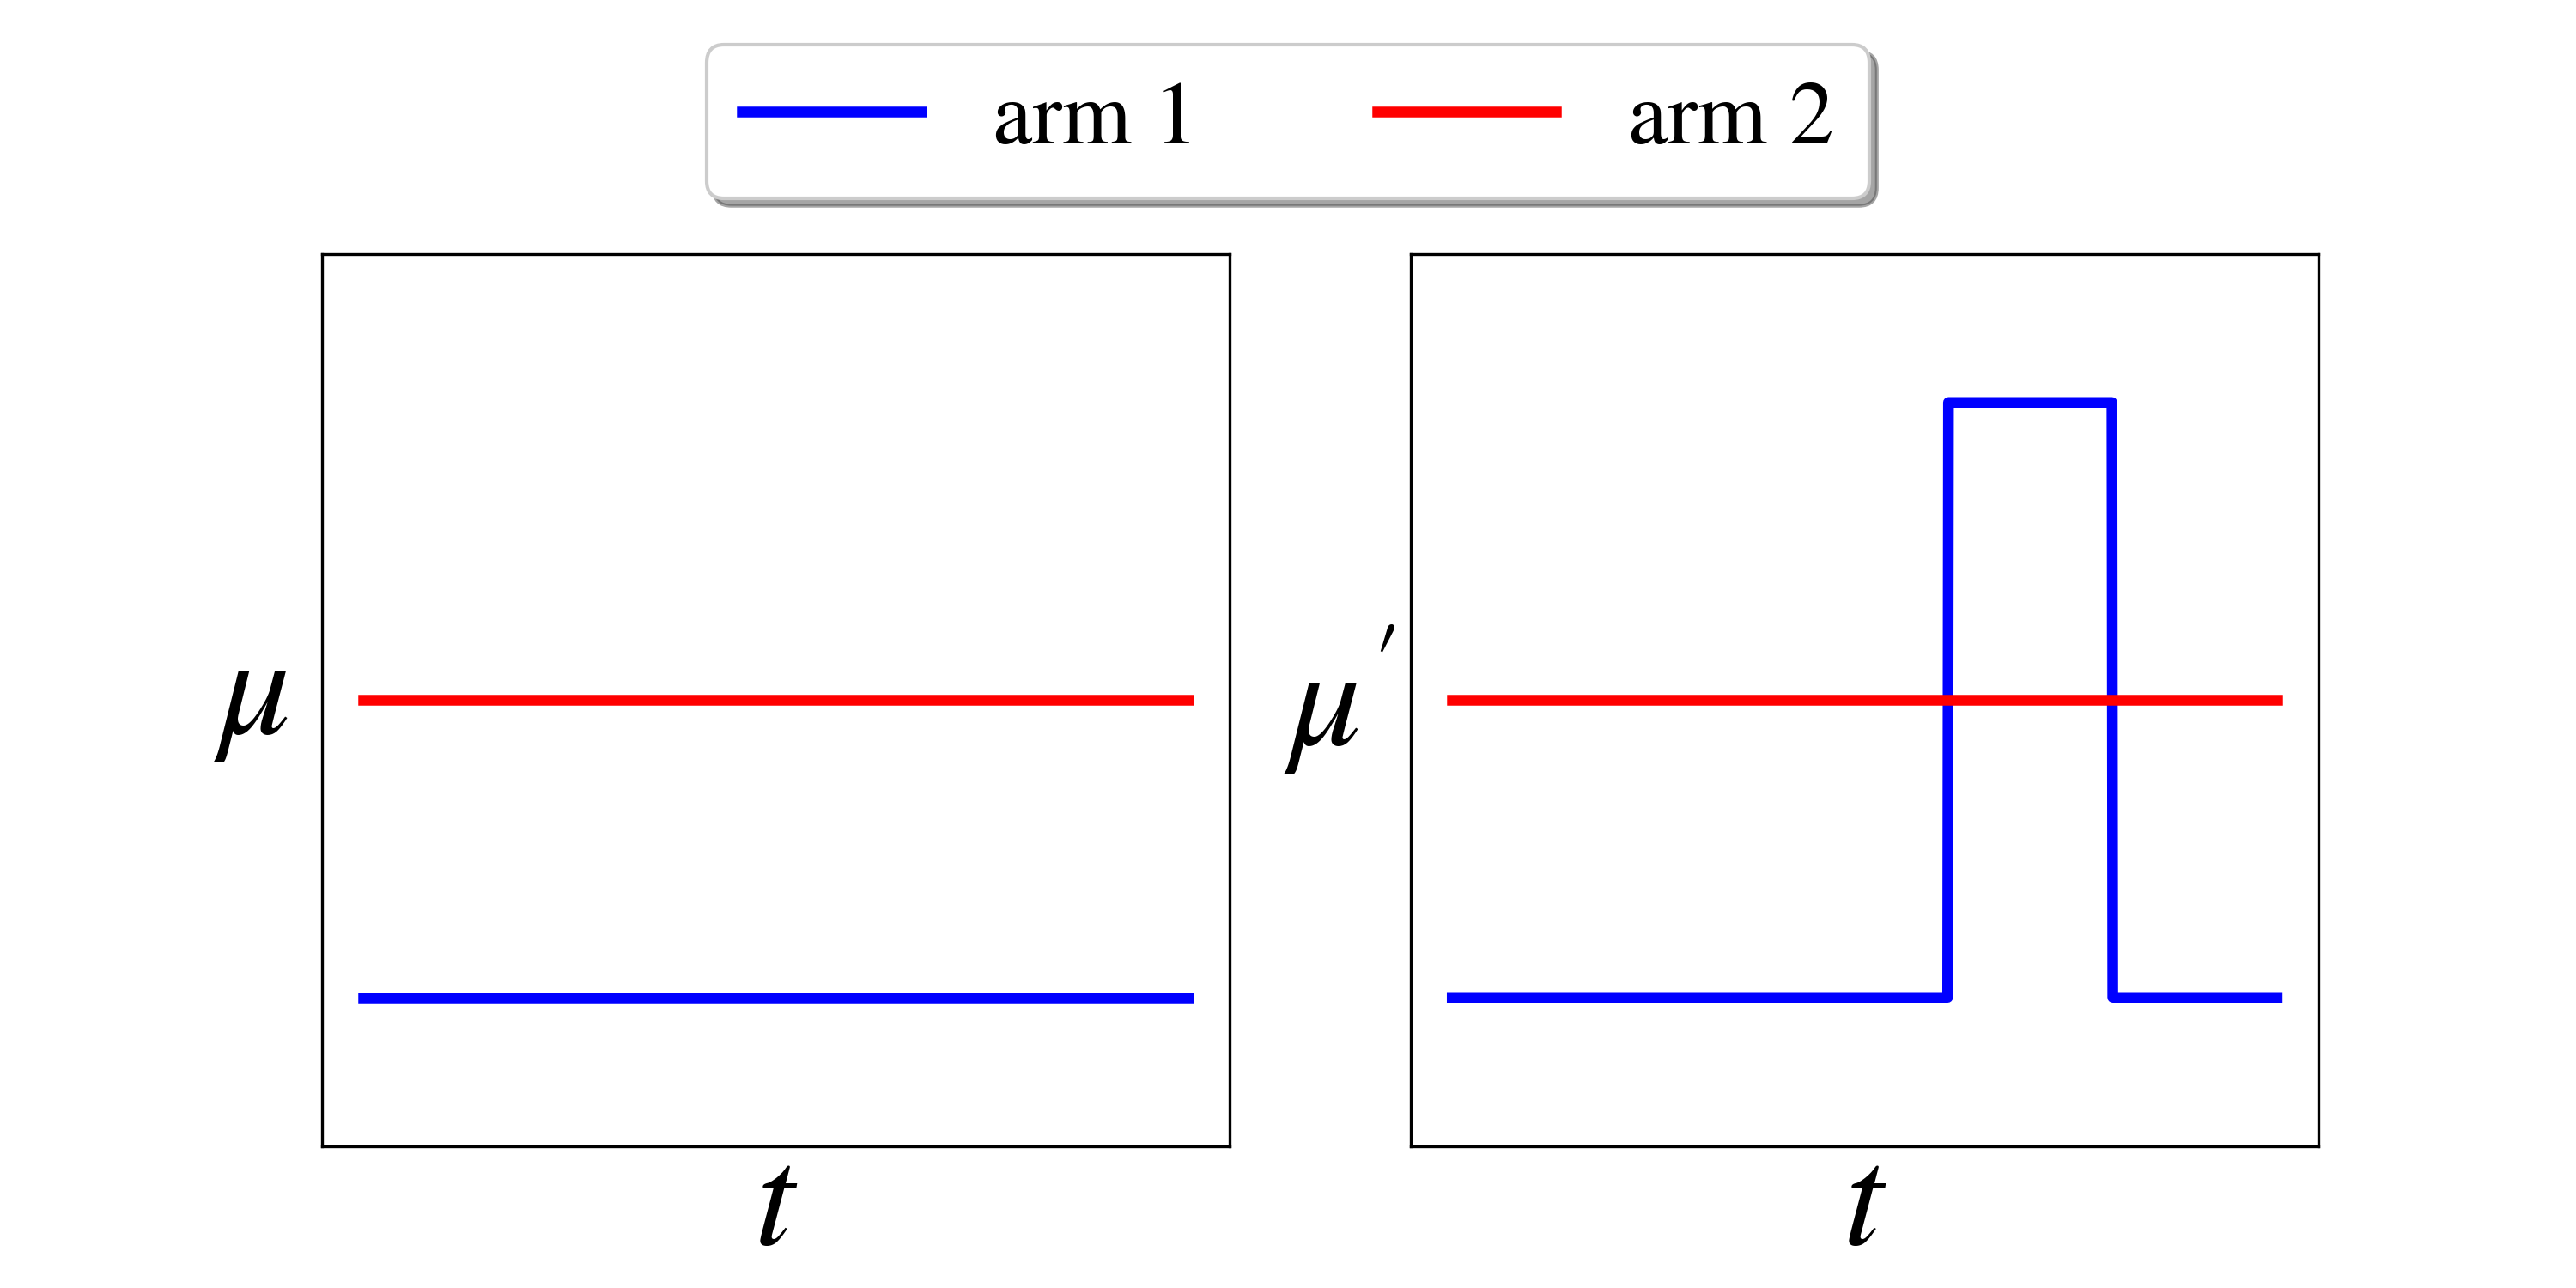
\includegraphics[clip, width= 0.99\textwidth]{4Restless/fig/garivier_lb.png}
\caption{The reward functions $\mu$ and $\mu'$. A policy with low regret on $\mu$ cannot achieve low regret on $\mu'$.}
\label{fig:garivier-lb}
\end{figure*}

\begin{proposition}[Theorem~31.2, \citet{lattimore2020banditbook}]
\label{prop:garivier-lb}
If a policy $\pi$ performs a regret $R_T(\pi, \mu)$ on a 2-arm stationary instance $\mu$, one can find a piece-wise stationary instance $\mu'$ with only two breakpoints such that, for a sufficiently long horizon $T$, the regret is lower bounded by 
\[\EE{R_T(\pi, \mu')} \geq \frac{T}{22R_T(\pi, \mu)}\,\cdot\]  
\end{proposition}

\begin{corollary}
\label{cor:garivier-lb}
Let $\pi$ a minimax optimal policy on the piece-wise stationary setups. Then, for a sufficiently large horizon $T$, there exists a universal constant $C$ such that for all the 2-arm stationary problems $\mu$, 
\[
\EE{R_T(\pi,\mu)} \geq C\sqrt{T}.
\]
\end{corollary}

These results state that one cannot have simultaneously a near-optimal problem-dependent regret rate $\cO\pa{\log{T}}$ on stationary instances and the minimax optimal piece-wise stationary rate $\cO\pa{\sqrt{T}}$. It is very different from the stationary case (or even with the rested rotting bandits presented in the last section) where some algorithms are shown to perform optimally both problem-dependent and problem-independent wise \citep{lattimore2018refining, menard2017klucb++}.

\subsubsection{Policies for piece-wise stationary bandits.}
\paragraph{Softmax policies.} For any sequence generated by an oblivious adversary, \EXPS \citep{auer2002nonstochastic} - an extension of \EXP - is guaranteed to achieve $\cO\pa{\sqrt{K\Upsilon_T T\log\pa{KT}}}$ regret against the best policy among the ones which change arms at most $\Upsilon_T -1$ times. The bound holds in the special case where the adversary generates the reward with noisy piece-wise stationary functions. In that case, the pseudo-regret definition is equivalent to the piece-wise stochastic regret defined in Equation~\ref{eq:restless-regret}. Indeed, the optimal policy is included in the set of $\cO\pa{\pa{KT}^{\Upsilon_T}}$ policies with at most $\Upsilon_T-1$ change of arms. 

\paragraph{Passive forgetting policies.} \DUCB \citep{kocsis2006discounted} and \SWUCB \citep{garivier2011upper-confidence-bound} are two ucb index policies which forget the older sample either by a discount factor or by a sliding window mechanism. The confidence interval increases when an arm has not been pulled for many rounds. When they are adequately tuned, these policies achieve respectively $\cO\pa{\sqrt{K\Upsilon_T T}\log{T}}$ and $\cO\pa{\sqrt{K\Upsilon_T T \log{T}}}$ minimax regret rate. While these policies do not improve the rate of \EXPS, they are deterministic and more explainable. 

\paragraph{Change-detection policies.} Instead of throwing away old samples at a fixed pace, one could remove samples from the index only when they notice a change in the arm's mean. This is the spirit of the Change-Detection ucb algorithms. These algorithms have three components: an ucb index, a change-detection subroutine, and a fixed active exploration rate (either deterministic or random pulls). The active exploration rate is meant to detect the arms which change from suboptimal value to optimal ones (like in Figure~\ref{fig:garivier-lb}). The optimal budget dedicated to active exploration scales with $\cO\pa{\sqrt{K\Upsilon_T T}}$. %When $\Upsilon_T$ is unknown, one can set a count $\Upsilon$ to $1$ and increases it at each detected change. 

\MUCB \citep{cao2019nearly} uses a simple change detector which compares the average of the last $\nicefrac{w}{2}$ samples with the average of the before last $\nicefrac{w}{2}$ ones and check whether the difference is significant or not. The optimal tuning of the parameter $w$ depends on the value of $\Upsilon_T$: if changes are large and frequent, one should choose a small value of $w$; if changes are small and sparse, one should choose a large value of $w$.

\CUSUMUCB \citep{liu2018change-detection} uses a change detector which constructs two random walks based on the upper and lower deviation of the new samples compared to the mean of the $M$ first ones. If one of the random walks reaches a threshold $h$, then the change detector triggers. The random walks are negatively biased with a small value $\epsilon$ to prevent the natural deviation to trigger the change detector. Again, the optimal value of the parameters $M$, $\epsilon$ and $h$ depends on the number of changes $\Upsilon_T$.

\GLRUCB \citep{besson2019generalized} uses the Gaussian Likelihood Ratio change detector. This change detector scans all the samples to detect any size of change on any period with high probability. The probability parameter only needs the knowledge of the horizon $T$ to achieve near-optimal minimax bound. \citet{mukherjee2019distribution} introduces a very similar algorithm but study the assumption where all the arms change their value significantly at each breakpoint. With this assumption, they do not need active exploration and recover problem-dependent bound $\cO\pa{\log{T}}$.

On the theoretical side, the analysis often assumes that each change is large enough to be detected before the next change. Indeed, after the detection of the breakpoint, they use the analysis of \UCB on each stationary batch. Before the change detection, they do not provide any non-trivial bound on the quality of the selected arm. 


\paragraph{Agnostic policies.}
\citet{auer2019adaptively} consider the problem with no assumption on the change-point detectability. They propose \ADSWITCH, which also uses a parameter-free change-detection subroutine but with an elimination policy: it pulls arms in a round-robin way a refined set of good arms. Arms are excluded from this set when they demonstrate with high probability that they underperform. The bad arms are also actively explored with consecutive sampling: the algorithm selects at random an arm and a deviation size $\Delta$ and pulls the arm the right number of rounds to detect if there is a change of size $\Delta$ in the arm's value. \citet{chen2019new} extend this technique to the contextual bandits problem.

A previous attempt \citep{cheung2019new} to solve this problem uses an expert aggregation bandit algorithm (e.g. \EXPfour) to select between different tuning of \SWUCB . Yet expert aggregation of bandit algorithm is problematic \citep{agarwal2017corralling, besson2018aggregation}, and \citet{cheung2019new} has to run each copy by batch with full restart. This technique leads to a suboptimal rate $\tcO\pa{\sqrt{K \max\pa{\Upsilon_T, \sqrt{T}} T}}$.


\subsection{Variation budget bandits}
\label{subsec:variation}
\citet{besbes2014stochastic} introduce the limited variation budget bandits, a restless setting where at each round Nature can modify the reward value of any arm but with a limited total variation budget $V_T$ at the round $T$. 

\begin{assumption}
\label{assum:variation}
$\mu_i : \NN^\star \rightarrow [- V_T, 0]$ are functions of the time $t$ with $V_T$ a positive constant. Moreover, we have that 
\begin{equation}
\label{eq:defbudget}
    \sum_{t=1}^{T-1} \sup_{i \in \arms} |\mu_i(t+1) - \mu_i(t) | \leq V_T\,.
\end{equation}
\end{assumption}


\paragraph{Lower Bound}
\begin{proposition}[\citet{besbes2014stochastic}]
\label{prop:variation_lb}
For any strategy $\pi$, there exists a  variation budget bandit scenario with means $\{\mu_i(t)\}_{i,t}$ satisfying Assumption~\ref{assum:variation} with a budget $V_T \geq \sigma \sqrt{\frac{K}{8T}}$ such that
%
\[
    \mathbb{E}\left[R_T(\pi)\right] \geq \frac{1}{16\sqrt{2}} \pa{\sigma^2 V_T KT^2}^{1/3}.
\]
\end{proposition}

In the next section, we prove a stronger statement, using only non-increasing reward functions. Yet, there is no additional difficulty. While the two Assumptions~\ref{assum:piece-wise} and~\ref{assum:variation} leads to different regret rate (see Proposition~\ref{prop:piecewise_lb}), the proof (see e.g. Lemma~\ref{lemma:lb} in the next subsection) shows that there is a strong similarity between the two problems, at least from a minimax perspective.

\paragraph{Policies for variation budget bandits.}
Most of the algorithms presented for the piece-wise stationary case are also near-optimal for the variation budget case. Indeed, \citet{besbes2014stochastic} show that \EXPS also learns in the variation budget setup. They also present \REXP, an algorithm based on \EXP with periodic restart which recovers a similar guarantee than \EXPS. \citet{cheung2019new} and \citet{russac2019weighted} extend \SWUCB and \DUCB to the linear bandit setting with variation budget. \citet{chen2019new} proves that \ADSWITCH is also optimal in the variation budget setting. However, change-detection ucb algorithms are not proved to perform well in the variation budget setting. Indeed, their proofs use the proof of \UCB on each stationary batch. In the variation budget setup, there is no stationary batch, which makes these algorithms harder to analyze. 

\subsection{The restless rotting assumption}
\label{subsec:restless-rotting}
\begin{assumption}
\label{assum:restless_rotting}
Reward functions $\left\{\mu_i \right\}_i$ are non-increasing with $t$.
\end{assumption}
We use this Assumption with Assumption~\ref{assum:piece-wise} and~\ref{assum:variation}.
\begin{remark}
\label{remark:budget}
With the rotting assumption, the variation budget assumption is very similar to the bounded assumption. Indeed, any set of decreasing functions $\mu_i : \NN^\star \rightarrow [- V, 0]$ satisfies Equation~\ref{eq:defbudget} with $V_T = KV$. Reciprocally, any set of functions satisfying Equation~\ref{eq:defbudget} with $\mu_i(1) \in [- V_T, 0]$ are bounded in $[- 2V_T, 0]$. 
\end{remark}

\paragraph{Lower bounds.} We show that our additional decreasing assumption does not change the minimax rates of the two settings. This is an adaptation of the proof of \citet{besbes2014stochastic} where we only use rotting functions.

\begin{restatable}{proposition}{restapiecewiselb}
\label{prop:piecewise_lb2}
For any strategy $\pi$, there exists a \underline{rotting} piece-wise stationary bandit scenario with means $\{\mu_i(t)\}_{i,t}$ \underline{satisfying Assumptions~\ref{assum:piece-wise} and~\ref{assum:restless_rotting}} with $\Upsilon_T\! \leq \!\pa{\!\frac{32V^2T }{K\sigma^2}\!}^{\!\nicefrac{1}{3}\!}\!$ such that,
\[
    \mathbb{E}\left[R_T(\pi)\right] \geq \frac{\sigma}{32}\sqrt{ \Upsilon_T KT}\,.
\]
\end{restatable}
\begin{restatable}{proposition}{restavariationlb}
\label{prop:variation_lb2}
For any strategy $\pi$, there exists a \underline{rotting} variation budget bandit scenario with means $\{\mu_i(t)\}_{i,t}$ \underline{satisfying Assumptions~\ref{assum:variation} and~\ref{assum:restless_rotting}} with a budget $V_T \geq \sigma \sqrt{\frac{K}{8T}}$ such that,
%
\[
    \mathbb{E}\left[R_T(\pi)\right] \geq \frac{1}{16\sqrt{2}} \pa{\sigma^2 V_T KT^2}^{\nicefrac{1}{3}}.
\]
\end{restatable}

The condition on $\Upsilon_T$ in Proposition~\ref{prop:piecewise_lb2} follows from Remark~\ref{remark:budget}: if $V$ is too small compared to $\Upsilon_T$, then we have a budget constraint - with associated lower bound in Proposition~\ref{prop:variation_lb2} - rather than a breakpoint constraint.


\paragraph{Proof}
 Our proof build a set of rotting piece-wise stationary problems with an evenly spaced set of $\Upsilon -1$ breakpoints. The adversary can choose the distance between arms $\Delta=\frac{1}{4} \sqrt{\frac{\sigma^{2} K \Upsilon}{2 T}}$ at the maximum such that the best arm is barely identifiable between two breakpoints (see Lemma~5.1, \citet{auer2002nonstochastic}). At each breakpoint, each arm's value decreases by $\Delta$ or $2\Delta$. Even if the set of breakpoints would be known, the learner does not know which arm is the best on each stationary part. Hence, in the worst case, she suffers at least the sum of the minimax regret of $\Upsilon$ stationary bandits problems with horizon $\frac{T}{\Upsilon}$, \textit{i.e.}  $\cO \pa{\sqrt{K\Upsilon T}}$. In the piece-wise stationary setting, we can simply identify $\Upsilon = \Upsilon_T$. In the variation budget setting, the adversary has a constraint over $\Upsilon \Delta = \frac{1}{4} \sqrt{\frac{\sigma^{2} K \Upsilon^3}{2 T}}=  \cO\pa{V_T}$. Hence, when the budget is limited, the adversary can choose up to $\Upsilon = \cO\pa{ T^{1/3}}$ breakpoints such that the suboptimal arms are "sufficiently" far from the best one (\textit{i.e} at $\Delta$). This dependence on $T$ leads to the increased regret rate of $\cO\pa{T^{\nicefrac{2}{3}}}$.
 
\begin{lemma}\label{lemma:lb}
Let $\Upsilon \in \left\{1,\dots, T\right\}$ and $\left\{\tau_k \triangleq \ceil{\frac{T}{ \Upsilon}} \text{ if } k \leq T \bmod{\Upsilon} \text{ else } \floor{\frac{T}{ \Upsilon}}\right\}_{k\leq \Upsilon}$. We call $t_k = \sum_{k'=1}^k \tau_{k'}$ and $t_0 = 0$.  Consider a family of piece-wise stationary bandits indexed by a vector $i^\star\in (\{0\}\cup \arms)^{\Upsilon}$ as follows: arm $i$ is a Gaussian distribution $\mathcal{N}\pa{\mu_i(t), \sigma}$ such that 
\[
\forall k \in \left\{0 , \dots, \Upsilon -1 \right\}, \ \forall t \in \left\{t_{k-1}+1,\dots, t_{k}\right\}, \ 
\mu_i(t) = 
\begin{cases}
-k \Delta \text{ if } i = i^\star_k\\
-(k+1)\Delta  \text{ else.}
\end{cases}
\]
We denote by $\EEempty_{i^\star}$ the expectation under the problem indexed by $i^\star$. Then, if $\Delta = \frac{1}{4}\sqrt{\frac{\sigma^2K\Upsilon}{2T}}$, for any policy $\pi$ :
\[
 \exists i^\star\in (\{0\}\cup \arms)^{\Upsilon}, \  \EEempty_{i^\star}\big[R_T(\pi)\big]  \geq  \frac{\sqrt{\sigma^2KT\Upsilon}}{32}\cdot
\]
\end{lemma}
\begin{proof}
Note that when $i^\star_k = 0$ then all the arms share the same means. We also define the vector $i^\star_{-k}$ equals to $i^\star$ with the coordinate $k$ empty and for $i\in\arms$ the vector $(i^\star_{-k},i)$ as the vector where we fill the empty coordinate with $i$.  We fix a policy $\pi$ and we will lower bound its average regret on the bandits problem indexed by $i^\star \in \arms^\Upsilon$ 
\begin{align*}
    \frac{1}{K^{\Upsilon}} \sum_{i^\star\in \arms^{\Upsilon}}  \EEempty_{i^\star}\big[R_T(\pi)\big] &= \frac{1}{K^{\Upsilon}} \sum_{i^\star\in \arms^{\Upsilon}} \sum_{k=1}^{\Upsilon}\Delta \EEempty_{i^\star}[\tau_k - N_{i^\star_k}^k] \\
    &=\Delta \left(T - \frac{1}{K^{\Upsilon}} \sum_{i^\star\in \arms^{\Upsilon}} \sum_{k=1}^{\Upsilon} \EEempty_{i^\star}[N_{i^\star_k}^k]\right),
\end{align*}
where $N_i^k$ is the number of pulls of arm $i$ during epoch $k$. Thus we need to upper bound the following quantity
\[
\frac{1}{K^{\Upsilon}} \sum_{i^\star\in \arms^{\Upsilon}} \sum_{k=1}^{\Upsilon} \EEempty_{i^\star}[N_{i^\star_k}^k] = \sum_{k=1}^{\Upsilon} \frac{1}{K^{\Upsilon-1}} \sum_{i^\star_{-k}\in \arms^{\Upsilon-1}}\frac{1}{K} \sum_{i=1}^K\EEempty_{(i^\star_{-k},i)}[N_{i}^k]\,.
\]
Using the contraction of the entropy for the bounded random variable $N_{i}^k/\tau_k$ then the Pinsker inequality (see \citet{garivier2018explore}) we get
\[
2\left(\frac{1}{\tau_k K} \sum_{i=1}^K\EEempty_{(i^\star_{-k},i)}[N_{i}^k] -\frac{1}{\tau_k K} \sum_{i=1}^K\EEempty_{(i^\star_{-k},0)}[N_{i}^k] \right)^2 \leq \frac{1}{K} \sum_{i=1}^K \EEempty_{(i^\star_{-k},0)}[N_{i}^k] \frac{\Delta^2}{2\sigma^2}\CommaBin
\]
since problems $(i^\star_{-k},i)$ and $(i^\star_{-k},0)$ differ only by a gap $\Delta$ on the arm $i$ during epoch $k$. Thanks to the fact that  $\sum_i N_i^k \leq \tau_k$ we get 
\[
\frac{1}{K} \sum_{i=1}^K\EEempty_{(i^\star_{-k},i)}[N_{i}^k] \leq \frac{\tau_k}{K} + \frac{\Delta}{2\sigma \sqrt{K}}\tau_k^{\nicefrac{3}{2}}\,.
\]
Putting all together we have for $K\geq 2$
\begin{align*}
    \frac{1}{K^{\Upsilon}} \sum_{i^\star\in \arms^{\Upsilon}}  \EEempty_{i^\star}\big[R_T(\pi)\big]  \geq \left(\frac{T}{2} -  \sum_{k=1}^{\Upsilon} \frac{\tau_k^{\nicefrac{3}{2}} \Delta}{2\sigma \sqrt{K}}\right)\Delta\,.
\end{align*}
We have $\tau_k= \floor{\frac{T}{\Upsilon}}$ or $\tau_k= \ceil{\frac{T}{\Upsilon}}$  such that $\sum_{k=1}^{\Upsilon} \tau_k=T$. Hence, we have that $\tau_k \leq 2T/\Upsilon$ which leads to 
\[
 \frac{1}{K^{\Upsilon}} \sum_{i^\star\in \arms^{\Upsilon}}  \EEempty_{i^\star}\big[R_T(\pi)\big]  \geq  \left(\frac{1}{2}T - \frac{\sqrt{2}T^{\nicefrac{3}{2}}\Delta}{\sigma \sqrt{K\Upsilon}}\right)\Delta\,.
\]

Choosing $\Delta = \frac{1}{4}\sqrt{\frac{\sigma^2K\Upsilon}{2T}}$, we get 
\[
 \frac{1}{K^{\Upsilon}} \sum_{i^\star\in \arms^{\Upsilon}}  \EEempty_{i^\star}\big[R_T(\pi)\big]  \geq  \frac{1}{4}\sqrt{\frac{\sigma^2K\Upsilon}{2T}}\left(\frac{1}{4}T\right) \geq \frac{\sqrt{\sigma^2KT\Upsilon}}{32}\cdot
\]
We can conclude by noticing that the average expected regret across the problem set is lesser or equal to the maximum across the same problem set.
\end{proof}
\restapiecewiselb*
\begin{proof}
This result directly follows from Lemma~\ref{lemma:lb} by choosing $\Upsilon = \Upsilon_T$. Indeed, the set of problems $\left\{i^\star \in \left(\left\{0\right\} \cup \arms\right)^{\Upsilon_T} \right\}$ satisfy Assumptions~\ref{assum:piece-wise} and~\ref{assum:restless_rotting} as soon as $\Upsilon_T\Delta \leq V$, \ie $\Upsilon_T \leq \pa{\frac{32V^2T }{K\sigma^2}}^{\nicefrac{1}{3}}$.
\end{proof}

\restavariationlb*
\begin{proof}
\sloppy
We want to use Lemma~\ref{lemma:lb} but we need to make the set of problems $\left\{i^\star \in \left(\left\{0\right\} \cup \arms\right)^{\Upsilon_T} \right\}$ comply with Assumption~\ref{assum:variation}. First, the function are bounded by $-V_T$. Hence, we need : 
\begin{equation}
\label{eq:bounded_condition}
  \Upsilon \Delta \leq V_T.  
\end{equation}

Second, the total variation is bounded according to Equation~\ref{eq:defbudget}. When $t$ is not a breakpoint, the variation is null. At each breakpoint, the maximal variation across the arm is $2\Delta$. For $\Upsilon-1$ breakpoint, we have that 


\begin{equation}
\label{eq:totalvar_condition}
  2\Delta \pa{\Upsilon-1}  \leq V_T.  
\end{equation}

Since $ 2\Delta \pa{\Upsilon-1} \leq \frac{\sigma}{2}\sqrt{\frac{K}{2T}}\Upsilon^{\nicefrac{3}{2}} $, we choose 
\begin{equation}
\label{eq:set_upsilon}
\Upsilon = \min\pa{\max\pa{\floor{ 2\left(\frac{V_T^{2}T}{K\sigma^{2}}\right)^{\nicefrac{1}{3}}},1},T}.
\end{equation}

By construction, \ref{eq:set_upsilon} satisfies \ref{eq:totalvar_condition}. Moreover, when $\Upsilon >1$, \ref{eq:totalvar_condition} is more restrictive than \ref{eq:bounded_condition}. For $\Upsilon = 1$, we simply assume $\Delta \leq V_T$, \textit{i.e.} $V_{T} \geq \sigma \sqrt{\frac{K}{8 T}}$.

Plugging \ref{eq:set_upsilon} in Lemma~\ref{lemma:lb} allows us to conclude 
\[
    \mathbb{E}\left[R_T(\pi)\right] \geq \frac{1}{16\sqrt{2}} V_T^{\nicefrac{1}{3}}\sigma^{\nicefrac{2}{3}}K^{\nicefrac{1}{3}}T^{\nicefrac{2}{3}}.
\]
\end{proof}
%!TEX root = ../main.tex
\section{Analysis of adaptive window policies on restless rotting bandits.} 
\label{sec:restless-theory}
In Chapter~\ref{ch:rested}, we presented four adaptive window policies (\FEWA, \RAWUCB, \EFFFEWA, \EFFRAW). The proof of the regret upper bounds in the rested case uses three main steps. First, we design one favorable event per round on which all the constructed statistics concentrate on a well-chosen confidence region, such that it holds with sufficiently high probability. This part does not use that we faced a rested non-stationary environment; it only uses the concentration of independent subgaussian variables which remains true in our restless problem (see Equation~\ref{eq:restless-feedback}). Hence, we restate Propositions~\ref{prop:prb_favorable_event} and~\ref{prop:prb_favorable_event_eff},
\begin{proposition}
\label{prop:prb_favorable_event_full}
We recall that, for any round $t$ and confidence $\delta_{t} \triangleq 2t^{-\alpha}$, we define
%
\begin{align*}
&\!\HPevent\! \triangleq\! \Big\{ \forall i\!\in\!\arms,\ \forall n \!\leq\! t\!-\!1 ,\ \forall h \!\leq\! n, \big| \hmu^h_i(t, \pi) - \bmu^h_i(t, \pi) \big| \!\leq\! c(h, \delta_{t}) \!\Big\}\\
&\!\HPeff\! \triangleq\! \Big\{ \forall i\!\in\!\arms, \forall n \!\leq\! t\!-\!1 , \forall h_j \!\in\! \Him(n), \big| \hmueff(t,\pi) - \bmueff(t,\pi) \big| \!\leq\! c(h_j, \delta_{t}) \!\Big\}
\end{align*}
with  $c(h,\delta_{t}) \triangleq \sqrt{2 \subgaussian^2\log(2/\delta_t)/h}$. Then, for a policy $\pi$ which pulls each arms once at the beginning, and for all $t>K$,
\[
\PPempty\Big[\bar{\HPevent}\Big] \leq \frac{Kt^2\delta_{t}}{2}=Kt^{2-\alpha} \text{ and } \PPempty\Big[\bar{\HPeff}\Big] \leq 3Kt\delta_t= 6Kt^{1-\alpha}.
\]
\end{proposition} 

Then, we use the mechanics of the algorithms to relate the average past performance of the selected arm with the current best value of the arms. As we noticed in the proofs (see e.g. the proof of Lemma~\ref{lem:core-FEWA}), we do not use the rested aspect of the problem. In fact, these results hold for a more general reward function $\mu_i(t,n)$ which is non-increasing with both $t$ and $n$. Therefore, we also restate Lemmas~\ref{lem:core-FEWA}, \ref{lem:core-RAWUCB} and~\ref{lem:core-eff},
\begin{lemma}
\label{lem:core-full}
At any round $t$ on favorable event $\HPevent$ (respectively, $\HPtwo$), if arm~$i_{t}$ is selected by $\pi \in \left\{\piF, \piR\right\}$ (respectively, $\pi \in \left\{\piEF, \piER\right\} $ tuned with $m=2$), for any $h \leq \Nitmone$,  the average of its $h$ last pulls cannot deviate significantly from the best available arm at that round, i.e.,
\begin{equation*}
\bmu^{h}_{i_t}(t,\pi) \geq \max_{i \in \arms} \mu_{i}(t)- \frac{C_\pi}{\sqrt{2\alpha}} c(h, \delta_t) \quad \text{with } 
\begin{cases}
C_{\piR} = 2\sqrt{2\alpha} \text{ and } C_{\piER} = \frac{4\sqrt{\alpha}}{\sqrt{2}-1}\\
C_{\piF} = 4\sqrt{2\alpha} \text{ and }C_{\piEF} = \frac{8\sqrt{\alpha}}{\sqrt{2}-1}
\end{cases}\cdot
\end{equation*}
\end{lemma}
Last, we use a specific rested regret decomposition to show that our algorithms are near-optimal both problem-dependent and problem-independent wise on rested rotting bandits. Unfortunately, this part cannot be used for the restless analysis. However, with a specific restless regret decomposition (see the proof in Subsection~\ref{ss:restless-proof}), we can show that our policies matches the two aforementioned lower bounds up to poly-logarithmic terms without any knowledge of the horizon $T$ nor $\Upsilon_T$ or $V_T$.
%
\begin{restatable}{theorem}{restapiecewisetheorem}
\label{th:piecewise-minimax}
Let $\pi \in \left\{ \piF, \piR\right\}$ tuned with $\alpha \geq 4$ or $\pi \in \left\{ \piEF, \piER\right\}$ tuned with $\alpha \geq 3$ and $m=2$. For any piece-wise stationary bandit scenario with means $\{\mu_i(t)\}_{i,t}$ satisfying Assumptions~\ref{assum:piece-wise} and~\ref{assum:restless_rotting}  with $\Upsilon_T-1$ change-points, $\pi$  suffers an expected regret\,
\[
\EE{R_T(\pi)} \leq C_\pi \sigma \sqrt{\log{T}} \pa{ \sqrt{\Upsilon_T KT} + \Upsilon_T K} + 6KV.
\]
\end{restatable}
\vspace{-2em}
\begin{restatable}{theorem}{restabudgettheorem}
\label{th:variation-minimax}
Let $\pi \in \left\{ \piF, \piR\right\}$ tuned with $\alpha \geq 4$ or $\pi \in \left\{ \piEF, \piER\right\}$ tuned with $\alpha \geq 3$ and $m=2$. For any variation budget bandit scenario with means $\{\mu_i(t)\}_{i,t}$ satisfying Assumptions~\ref{assum:variation} and~\ref{assum:restless_rotting}  with variation budget $V_T$, $\pi$ suffers an expected regret\,
\[
\mathbb{E}\left[R_T(\pi)\right] \leq 4\pa{C_\pi^2 \sigma^2 V_T K T^2\log{T}}^{\nicefrac{1}{3}} \!+ 2\Big(C_\pi \sigma V_T^2  K^2  T \sqrt{\log{T}}\Big)^{\nicefrac{1}{3}} \!+ 6 V_T K.
\]
\end{restatable}
%
The remaining terms are of second-order when $KV_T \leq \cO{\pa{T}}$, which is a necessary condition for the problem to be learnable (see Proposition~\ref{prop:variation_lb2}). 
%
\paragraph{Are rotting restless bandits easier?} Learning at the minimax rate without knowing $\Upsilon_T$ or $V_T$ was achieved in the non-rotting setup by significantly more complex algorithms. For instance, \citet{auer2019adaptively} use a combination of filtering on the set of potentially good arms, forced exploration planning on identified bad arms, and full restart of the algorithm when a change is detected. This algorithmic complexity has a performance cost, as \ADSWITCH is guaranteed to achieve 56 times the leading term in Theorem~\ref{th:piecewise-minimax}. Moreover, these algorithms rely on doubling trick when the horizon is unknown, which also has a regret cost compared to intrinsically anytime algorithms \citep{besson2018doubling}.

Yet, Proposition~\ref{prop:piecewise_lb2}  and~\ref{prop:variation_lb2} show that the rotting assumption do not improve the minimax rate for the two considered setups. Interestingly both these lower bounds are matched by (tuned) \EXPS \citep{auer2002nonstochastic}, an algorithm originally designed for switching best arm in adversarial sequences of rewards. This is comparable to the fixed best arm world:  adversarial and stochastic bandits share the same minimax rate which is matched in both setups by \EXP. The main interest of the stochastic assumption is to allow for \textit{problem dependent analysis}. For the stochastic stationary bandits, it leads to a stronger $\cO{\pa{\log\pa{T}}}$ bounds. In the (non-rotting) piece-wise stationary setting, we argued in Subsection~\ref{subsec:piecewise} that the learner has to maintain $\cO\pa{\sqrt{T}}$ exploratory pulls to shield against increase of currently suboptimal arm (see Proposition~\ref{prop:garivier-lb} and Corollary~\ref{cor:garivier-lb}).

The decreasing Assumption~\ref{assum:restless_rotting} excludes the problems where suboptimal arms increases to become optimal from the set of possible problems. Theorem~\ref{th:piecewise_pd} shows that not only \RAWUCB is able to recover the $\cO\pa{\log\pa{T}}$ on stationary problems but also recovers the same rate on each batch of a rotting piece-wise stationary problem. 
\begin{restatable}{theorem}{restapiecewisetheorempd}
\label{th:piecewise_pd}
Let $\pi \in \left\{ \piF, \piR\right\}$ tuned with $\alpha \geq 4$ or $\pi \in \left\{ \piEF, \piER\right\}$ tuned with $\alpha \geq 3$ and $m=2$. For any piece-wise stationary bandit scenario with means $\{\mu_i(t)\}_{i,t}$ satisfying Assumptions~\ref{assum:piece-wise} and~\ref{assum:restless_rotting}  with $\Upsilon_T-1$ change-points, $\pi$ suffers an expected regret\,
\[
    \mathbb{E}\left[R_T(\pi)\right] \leq \sum_{k=0}^{\Upsilon_T-1} \sum_{i\in\arms} \frac{C_\pi^2 \sigma^2\log{T}}{\Delta_{i,k}} +  C_\pi \sigma \Upsilon_T K \sqrt{ \log{T}} + 6KV. 
\]
\end{restatable}
%TODO talk about tuning ?
%When $\Upsilon_T = 1$ (no changepoint), \RAWUCB recovers the same guarantee than \UCBone. However, \UCB with a more careful tuning $\delta_t \sim \frac{1}{t\log{t}^2}$ match \citet{lai1985asymptotically} asymptotic factor for Gaussian bandits \citep{lattimore2019bandit}. We leave the two following questions for future analysis: 1) Is there a tuning of $\delta_t$ such that \RAWUCB is asymptotic for stationary problems? 2) If yes, can \RAWUCB with this asymptotic tuning recovers some (rested or restless) non-stationary guarantees?

Notice that \citet{mukherjee2019distribution} use a different assumption to recover a similar problem-dependent bound. Indeed, they assume that all the arms change at the same time which also excludes $\mu'$ from the set of possible problems. %TODO
%Therefore, \RAWUCB is near minimax optimal \emph{and} reaches the asymptotic rate for stationary bandits $O(\sum_{i \in \arms} \frac{\log(T)}{\Delta_i})$ (see Corollary~\ref{dependent_theorem}) without knowing the number of change points nor the horizon. 

\subsection{Proofs}
\label{ss:restless-proof}

\subsubsection*{Sketch.} 

We start by separating the regret on the bad events $\bar{\HPevent}$ from the good events $\HPevent$. According to Proposition~\ref{prop:prb_favorable_event}, the bad events $\bar{\xi}_t$ have low probability for appropriate $\alpha$. For $\alpha = 4$, they weigh at most $\cO{\pa{KV}}$ in the expected regret.  On the good events, we write:
\vspace{-4pt}
\begin{equation}
\label{eq:restless-regret-decompo}
R_T(\pi)= \sum_{t=1}^T \mu_{i_t^\star}(t) - \bar{\mu}_{i_t}^{h_t}(t, \pi) + \bar{\mu}_{i_t}^{h_t}(t, \pi) - \mu_{i_t}(t).   
\end{equation}

Notice that Lemma~\ref{lem:core-full} can bound the first difference for any $h_t$. When the reward is piece-wise stationary, we can select $h_t$ such that we include all the pulls of arm $i_t$ from the current stationary batch. If there is none, then it is the first pull of arm $i_t$ in this batch. We handle these $\cO{\pa{K\Upsilon_T}}$ rounds separately (see Lemma~\ref{lem:FP}). In the other cases, we note that the second difference is null because $\bar{\mu}_{i_t}^{h_t}(t, \pi) = \mu_{i_t}(t) = \mu_i^k$ by the piece-wise stationary assumption. The remaining of the proofs of Theorem~\ref{th:piecewise-minimax} and~\ref{th:piecewise_pd} are then very similar to the analysis of \cite{auer2002finite} on each stationary batch. Indeed, Lemma~\ref{lem:core-full} is similar to the two confidence bounds guarantee of \UCBone's guarantee.

In the variation budget setting, there is no stationary batches. Hence, we cannot choose an $h_t$ which cancels the second difference in Equation~\ref{eq:restless-regret-decompo}. Yet, we still decompose the rounds in $\Upsilon$ batches of equal length for the analysis. We choose $h_t$ such that we include all the pulls of arm $i_t$ from the current batch. For the sum of the first differences in Equation~\ref{eq:restless-regret-decompo}, there is no difference with the piece-wise stationary case and we can bound
\vspace{-4pt}
\begin{equation}
\label{eq:variance_bound}
    \sum_{t=1}^T \mu_{i_t^\star}(t) - \bar{\mu}_{i_t}^{h_t}(t, \pi)\leq \tcO{\pa{\sqrt{K\Upsilon T}}}.
\end{equation}
We call $\Delta_i^k \triangleq \mu_i(t_k) - \mu_i(t_{k+1})$, the total variation of arm $i$ in batch $k$. The sum of second differences in Equation~\ref{eq:restless-regret-decompo} can be bounded as follows: on each batch of $T\Upsilon^{-1}$ rounds, each second difference is bounded by $\max_{i\in \arms} \Delta_i^k$. When we sum over the batches, we get
\vspace{-4pt}
\begin{equation}
\label{eq:bias_bound}
  \sum_{t=1}^T  \bar{\mu}_{i_t}^{h_t}(t, \pi) - \mu_{i_t}(t)\leq \frac{T}{\Upsilon}\sum_{k=0}^{\Upsilon-1}\max_{i \in \arms}\Delta_i^k  \leq \frac{TV_T}{\Upsilon}\, .  
\end{equation}
Indeed, in the middle term, we have a maximum on the summed variation of arm $i$ in batch $k$. On the right-hand side, we have $V_T$ which bounds the sum over the rounds of maximal variation of the arms (see Equation~\ref{eq:defbudget}). Thus, the right-hand side is larger because the maximum of sums is smaller than the sum of maximums. We can then choose $\Upsilon = \tcO{\pa{T^{\nicefrac{1}{3}}V_T^{\nicefrac{2}{3}}K^{\nicefrac{-1}{3}}}}$ to minimise the sum of Equations~\ref{eq:variance_bound} and ~\ref{eq:bias_bound}. It leads to the leading term of our Theorem~\ref{th:variation-minimax}. Notice that we still have to handle the first pull of each arm in each batch. If we bound roughly each first pull by $V_T$, we would get $K\Upsilon V_T \sim \tcO{\pa{V_T^{\nicefrac{5}{3}}}}$ which would be the leading term for large $V_T$. Our Lemma~\ref{lem:FP} is more careful such that it leads to a second order term when $KV_T \leq o\pa{T}$.

\subsubsection*{Full proof}
\begin{lemma}[Bound on unfavorable events. Decomposition in unspecified batches. Bound on the first pull of each arm in each batch] %TODO
\label{lem:FP}
Let an integer $\Upsilon \in\left\{ 1, \dots,T\right\}$.\\
Let $\mu_i : \NN^\star \rightarrow \left[0, -V\right]$, the $K$ decreasing reward functions.\\ 
Let $\left\{t_k\in\left\{ 1, \dots,T\right\} \right.\allowbreak\left. |\, t_k > t_{k-1}\right\}_{k\in \left\{ 1, \dots,\Upsilon-1\right\}}$ a set of $\Upsilon - 1$ distinct rounds delimiting $\Upsilon$ batches. We set $t_0=0$ and $t_\Upsilon = T$. \\
We call $h_{i}^{k} \triangleq \sum_{t=t_k +1}^{t_{k+1}} \mathbbm{1}\left(i_{t} = i\right)$ the number of pulls of arm $i$ in batch $k$ and $t_i^k(h)$ the time at which arm $i$ is pulled for the $h$-th time since $t_k + 1$. We also call $\arms_k \triangleq  \left\{ i \in \arms | h_i^k \geq 1\right\}$ the set of pulled arms in batch $k$. 

Then, $\pi \in \left\{\piR, \piF \right\}$ run with $\alpha \geq 4$, or $\pi \in \left\{\piER, \piEF \right\}$ run with $m=2$ and $\alpha \geq 3$, suffers an expected regret of
\begin{align*}
\EE{R_T(\pi)} \leq &  \, \EE{\sum_{k=0}^{\Upsilon-1} \sum_{i\in\arms_k}\sum_{t=t_k +1 }^{t_{k+1}}\sum_{h=2}^{h^k_{i}}\mathbbm{1}\pa{ t = t_i^k(h) \land \HPevent} \Big(\mu_{\star}(t) - \mu_{i}(t)\Big)} \\
&+   C_\pi \sigma \Upsilon K\sqrt{\log{T}} + 6KV.
\end{align*}
\end{lemma}
\begin{proof}
We start by separating the favorable events from the unfavorable events:
\begin{equation}
\label{eq:event_sep}
    R_T(\pi) = \underbrace{\sum_{t=1}^T \mathbbm{1}\pa{\HPevent} \pa{\mu_{\star}(t) - \mu_{i_t}(t)}}_{R_T(\pi | \HPevent)} + \underbrace{\sum_{t=1}^T \mathbbm{1}\big(\bar{\HPevent}\big) \pa{\mu_{\star}(t) - \mu_{i_t}(t)}}_{{R_T(\pi | \bar{\HPevent})}} \,,
\end{equation}
with $\mu_\star(t) \triangleq \max_{i\in\arms}\mu_i(t)$. For $\alpha \geq 4$, we can bound the cost of the unfavorable events thanks to Proposition~\ref{prop:prb_favorable_event_full},
\begin{equation}
\label{eq:bad_event}
    \EE {R_T(\pi | \bar{\HPevent})} \leq \sum_{t=1}^T \PP{\bar{\HPevent}} V  \leq \sum_{t=1}^T \frac{KV}{t^2} = \frac{KV\pi^2}{6} \leq 2KV.
\end{equation}

On the favorable events, given any ordered set of $\Upsilon -1$ breakpoints $\left\{t_k\right\}$, we divide the horizon in $\Upsilon$ batches $\left\{t_k+1, \dots, t_{k+1} \right\}_{k \leq \Upsilon-1}$, 
\[
R_T(\pi | \HPevent) \leq \sum_{k=0}^{\Upsilon-1} \sum_{t=t_{k} +1 }^{t_{k+1}} \mathbbm{1}\pa{\HPevent} \big(\mu_{\star}(t) - \mu_{i_t}(t)\big).
\]
We define $h_{i}^{k}$ the number of pulls of arm $i$ in batch $k$, \textit{i.e.}  $h_{i}^{k} = \sum_{t=t_k +1}^{t_{k+1}} \mathbbm{1}\left(i_{t} = i\right)$. We use $t_i^k(h)$ to designate the time at which arm $i$ is pulled for the $h$-th time since $t_k$.
\[
R_T(\pi | \HPevent) \leq \sum_{k=0}^{\Upsilon-1} \sum_{t=t_k +1 }^{t_{k+1}} \sum_{i\in\arms_k} \sum_{h=1}^{h^k_{i}} \mathbbm{1}\pa{t_i^k(h) = t \land \HPevent} \Big(\mu_{\star}(t) - \mu_{i}(t)\Big).
\]
We split the regret on the first pulls of each batch,
\begin{align}
\label{eq:fp_op}
\begin{split}
    R_T(\pi | \HPevent) = & \underbrace{\sum_{k=0}^{\Upsilon-1}\sum_{t=t_{k} +1 }^{t_{k+1}} \sum_{i\in\arms_k} \mathbbm{1}\pa{t = t_i^k(1) \land \HPevent}\Big(\mu_{\star}(t) - \mu_{i}(t)\Big)}_{FP} \\ & +  \underbrace{\sum_{k=0}^{\Upsilon-1}\sum_{t=t_{k} +1 }^{t_{k+1}} \sum_{i\in\arms_k} \sum_{h=2}^{h^k_{i}}\mathbbm{1}\left( t = t_i^k(h) \land \HPevent \right)\Big( \mu_{\star}(t) - \mu_{i}(t)\Big)}_{OP} .
\end{split}
\end{align}

\paragraph{Analysis of the first pulls.}

We call $k_i^1$, the index of the batch at which arm $i$ is pulled for the first time.  We call $\arms_k^2 \triangleq \left\{ i \in \arms_k | k > k_i^1\right\}$, the set of arms pulled at least once during batch $k$ and at least once in a batch before $k$. We split the regret due to the very first pull each arm from the other first pulls in each batch,
\begin{align*}
FP  = &\sum_{k=0}^{\Upsilon-1}\sum_{i\in\arms_k}\sum_{t=t_{k} +1 }^{t_{k+1}}  \mathbbm{1}\pa{ t = t_i^k(1) \land \HPevent}\Big(\mu_{\star}(t) - \mu_{i}(t)\Big)\\
\leq& \sum_{i \in \arms}  \Big(0- \mu_i(t_i^{k_i^1}(1))\Big) +  \sum_{k=1}^{\Upsilon -1} \sum_{i\in \arms_k^2}\sum_{t=t_k +1 }^{t_{k+1}}  \mathbbm{1}\pa{t = t_i^k(1) \land \HPevent}\Big(\mu_{\star}(t) - \mu_{i}(t)\Big)\\
 =& \sum_{i \in \arms} \Big(0- \mu_i(t_i^{k_i^1}(1))\Big) \\
& + \sum_{k=1}^{\Upsilon -1} \sum_{i\in \arms_k^2} \sum_{t=t_k +1 }^{t_{k+1}}  \mathbbm{1}\pa{ t = t_i^k(1) \land \HPevent}\Big(\mu_{\star}(t) - \bar{\mu}^1_i(t, \pi) + \bar{\mu}^1_i(t,\pi) - \mu_{i}(t)\Big).
\end{align*}

The inequality is justified because $\mu_i(t) \leq 0$ for all $t$. In the last equation, we simply introduce $\bar{\mu}^1_i(t,\pi)$, the last pulled sample of arm $i$, which is well defined after the first pull of each arm.
According to Lemma~\ref{lem:core-full}, the first difference is bounded on the high-probability event $\HPevent$,
\begin{equation}
    \label{eq:fp_lemma1}
    \sum_{t=t_k +1 }^{t_{k+1}} \mathbbm{1}\pa{t = t_i^k(1) \land \HPevent}\pa{\mu_{\star}(t) - \bar{\mu}^1_i(t, \pi)} \leq \frac{C_\pi}{\sqrt{2\alpha}} c(1,2T^{-\alpha}) = C_{\pi} \sigma \sqrt{\log{T}}.
\end{equation}


We will show that we can telescope the second sum. First, we notice that we can collapse the sum on $t$ using $ \mathbbm{1}\pa{t = t_i^k(1)}$. Moreover, $\HPevent$ will not be needed: hence we can drop $\mathbbm{1}\pa{\HPevent} \leq 1 $.
\begin{equation}
\label{eq:fp_collapse}
 \sum_{t=t_k +1 }^{t_{k+1}} \mathbbm{1}\pa{ t = t_i^k(1) \land \HPevent}\pa{\bar{\mu}^1_i(t,\pi) - \mu_{i}(t)} \leq \bar{\mu}^1_i(t_i^k(1), \pi) - \mu_{i}(t_i^k(1)).
\end{equation}

For a given batch $k$ on which arm $i$ is pulled, the precedent reward sample has a mean $\bar{\mu}_i^h\pa{t_i^k\pa{1}, \pi}$. This sample is the last pull of the last batch $k'$ before $k$ on which arm $i$ is pulled. Hence, its mean is smaller than the mean of the first pull on this same batch $k'$ because the reward is decreasing. Hence, the sum can telescope
\begin{align}
\label{eq:fp_telescoping} 
\sum_{i \in \arms} \Big(0 -& \mu_i(t_i^{k_i^1}(1))\Big) + \sum_{k=1}^{\Upsilon -1}  \sum_{i\in \arms_k^2} \sum_{t=t_k +1 }^{t_{k+1}}\mathbbm{1}\pa{ t = t_i^k(1) \land \HPevent}\pa{ \bar{\mu}^1_i(t,\pi) - \mu_{i}(t)} \nonumber\\
& \leq \sum_{i \in \arms}\left\{ 0- \mu_i(t_i^{k_i^1}(1)) + \sum_{k=k_i^1 + 1}^{\Upsilon-1 } \mathbbm{1}\pa{h^k_{i} \geq 1  }\pa{\bar{\mu}^1_i(t_i^k(1), \pi) - \mu_{i}(t_i^k(1))} \right\} \nonumber\\
& \leq \sum_{i \in \arms} \Big(0-\mu_i(T)\Big) \leq KV\,.  
\end{align}
The first inequality uses the definition of $\arms_k^2$ along with Equation~\ref{eq:fp_collapse}. The second inequality follows from the telescoping argument presented above. The third inequality uses that $\mu_i(T) \geq -V$. Gathering Equation~\ref{eq:fp_lemma1} and  ~\ref{eq:fp_telescoping}, we can bound the term $FP$ (defined in Equation~\ref{eq:fp_op}) 
\begin{equation}
\label{eq:fp_bound}
FP \leq  KV + \sum_{k=1}^{\Upsilon - 1} \sum_{i\in \arms_k^2} C_\pi \sigma \sqrt{\log{T}} \leq KV + C_\pi \sigma \Upsilon K\sqrt{\log{T}} .    
\end{equation}



\paragraph{Conclusion.} From Equation~\ref{eq:event_sep}, we can bound the expected regret on the unfavorable events thanks to Equation~\ref{eq:bad_event}. On the favorable events, we can split the rounds in batches on which we isolate the first pull of each arm on each batch thanks to Equation~\ref{eq:fp_op}. Finally, we bound the regret due to these first pulls thanks to Equation~\ref{eq:fp_bound}, and for $\alpha \geq 4$,
\begin{align*}
\EE{R_T(\pi)} \leq &  \, \EE{\sum_{k=0}^{\Upsilon-1} \sum_{i\in\arms_k}\sum_{t=t_k +1 }^{t_{k+1}}\sum_{h=2}^{h^k_{i}}\mathbbm{1}\pa{ t = t_i^k(h) \land \HPevent} \Big( \mu_{\star}(t) - \mu_{i}(t)\Big)} \\
&+  C_\pi \sigma \Upsilon K \sqrt{\log{T}} + 3KV.
\end{align*}

For the efficient algorithms, we can use the same proof with $\HPtwo$ and get for $\alpha \geq 3$, 
\begin{align*}
\EE{R_T(\pi)} \leq &  \, \EE{\sum_{k=0}^{\Upsilon-1} \sum_{i\in\arms_k}\sum_{t=t_k +1 }^{t_{k+1}}\sum_{h=2}^{h^k_{i}}\mathbbm{1}\pa{ t = t_i^k(h) \land \HPevent} \Big(  \mu_{\star}(t) - \mu_{i}(t)\Big)} \\
&+  C_\pi \sigma \Upsilon K \sqrt{\log{T}} + 6KV.
\end{align*}

\end{proof}

\begin{lemma}[Analysis of the second pulls in each batch under the favorable events.]\label{lem:OP}
Let $\Delta_i^k \triangleq \mu_i(t_k+1) - \mu_i(t_{k+1})$, the decrement of arm $i$ in batch $k$. For any arm $i$ and any consecutive rounds $\left\{t_k+1, \dots , t_{k+1}\right\}$ such that $i$ is pulled $h_i^{k} \geq 1$ times, the regret due to the pulls after the first one can be bounded under the favorable events, 
\begin{multline*}
\sum_{t=t_{k} +1 }^{t_{k+1}} \sum_{h=2}^{h^k_{i}}\mathbbm{1}\left(t = t_i^k(h) \land \HPevent \right)\Big(  \mu_{\star}(t) - \mu_{i}(t)\Big) \\ \leq  \pa{h_i^k-1}\Delta_i^k + \sum_{h=2}^{h^k_{i}}\mathbbm{1}\left(\HPt{t_i^k(h)}\right)\pa{  \mu_{\star}(t_i^k(h)) - \bar{\mu}_i^{h-1}(t_i^k(h),\pi)} .
\end{multline*}
\end{lemma}
\begin{proof}
We call $\Delta_{i}(t,t')\triangleq \mu_i(t) - \mu_i(t')$ the variation of arm $i$ between times $t$ and $t'$.
As a short notation, we refer to $\Delta_i^k \triangleq \Delta_{i}(t_k+1,t_{k+1})$ for the variation of arm $i$ in batch $k$.

\begin{equation}
\label{eq:batch_delta_var}
    \forall h\leq h_i^k, \quad \mu_i( t_i^k(h)) \geq \mu_i(t_{k+1}) =  \mu_i(t_k +1 ) - \Delta_i^k \geq \bar{\mu}_i^{h-1}( t_i^k(h), \pi) - \Delta_i^k\,.
\end{equation} 
The two inequalities are justified by the rewards decay. Indeed, any pull in batch $k$ has a higher reward than the value of arm $i$ at the end of the batch $t_{k+1}$. Moreover, the value at the beginning of the batch is higher that any average of $h$ value in this batch. The middle equality follows from the definition of $\Delta_i^k$.

Then, we plug Equation~\ref{eq:batch_delta_var} in the left hand side of our claim,
\begin{align*}
\sum_{t=t_{k} +1 }^{t_{k+1}}
\sum_{h=2}^{h^k_{i}}\mathbbm{1}&\left(t = t_i^k(h) \land \HPevent\right)\Big(  \mu_{\star}(t) - \mu_{i}(t) \Big) \\
& = \sum_{h=2}^{h^k_{i}}\mathbbm{1}\left(\HPt{t_i^k(h)}\right)\pa{  \mu_{\star}(t_i^k(h)) - \mu_{i}(t_i^k(h))} \\
&\leq \sum_{h=2}^{h^k_{i}}\mathbbm{1}\left(\HPt{t_i^k(h)}\right)\pa{  \mu_{\star}(t_i^k(h)) - \bar{\mu}_i^{h-1}( t_i^k(h),\pi) + \Delta_i^k}\\
&\leq  \pa{h_i^k-1}\Delta_i^k + \sum_{h=2}^{h^k_{i}}\mathbbm{1}\left(\HPt{t_i^k(h)}\right)\pa{  \mu_{\star}(t_i^k(h)) - \bar{\mu}_i^{h-1}(t_i^k(h),\pi)} .
\end{align*}
The last inequality is justified by $\mathbbm{1}\left(\HPt{t_i^k(h)}\right)\leq 1$.
\end{proof}

\subsubsection*{Piecewise stationary rotting bandits.}
\sloppy
Let $\left\{t_k\right\}_{\left\{k \leq \Upsilon_T\right\}}$ be the set of breakpoints with $t_0=0$ and $t_{\Upsilon_T} = T$. For all $t \in \left\{t_k\! +\!1 , \dots , t_{k\!+\!1}\right\}$, $\mu_i(t) = \mu_i^k$. We denote $i^\star_k \in \argmax_{i\in \arms} \mu_i^k$ (one of) the best arm(s) in batch $k$, and $\mu_{\star}^k \triangleq \max_{i\in \arms} \mu_i^k$, the corresponding best value. We also call $\Delta_{i,k} \triangleq \mu_{\star}^k - \mu_i^k$ the gap between arm $i$ and optimal arm in batch $k$.

\begin{lemma}
\label{lem:OP-piecewise}
For an arm $i$ and a stationary batch $k$, we call $h_{i,\xi}^k \triangleq \max\left(h \leq h_i^k | \HPt{t_i^k(h)} \right)$ the last pull of arm $i$ in batch $k$ under the favorable events (possibly 0). If $h_{i,\xi}^k \geq 1$, the regret due to the second pulls on the favorable events is bounded by,
\[
\sum_{t=t_{k}+1}^{t_{k+1}} \sum_{h=2}^{h_{i}^{k}} \!\mathbbm{1}\!\pa{\! t=t_{i}^{k}(h) \land \HPevent \!}\!\Big(\!\mu_{\star}(t)\!-\!\mu_{i}(t)\!\Big) \leq\pa{\!h_{i, \xi}^{k}\!-\!1 \!} \Delta_{i, k} \leq C_\pi\sigma \sqrt{\pa{\!h_{i,\xi}^k\!-\!1\!}\log{T}}.
\]
\end{lemma}
\begin{proof}
We apply Lemma~\ref{lem:OP} on each stationary batch. Hence, $\Delta_i^k =0$ and we can write,
%
\begin{equation*}
\!\sum_{t=t_{k} +1 }^{t_{k+1}}\! \sum_{h=2}^{h^k_{i}} \! \mathbbm{1}\left(\!t = t_i^k(h) \land \HPevent \!\right)\Big(\! \mu_{\star}(t) - \mu_{i}(t)\!\Big) \leq   \sum_{h=2}^{h^k_{i}} \!\mathbbm{1}\left(\!\HPt{t_i^k(h)}\!\right)\pa{\!  \mu_{\star}(t_i^k(h)) - \bar{\mu}_i^{h-1}(t_i^k(h),\pi)\!}\! .
\end{equation*}

We notice that $\mu_{\star}(t_i^k(h)) = \mu_{\star}^{(k)}$. We call $h_{i,\xi}^k \triangleq \max\left(h \leq h_i^k\, \,| \HPt{t_i^k(h)} \right)$. Hence,
\begin{align*}
\sum_{h=2}^{h^k_{i}}\!\mathbbm{1}\left(\HPt{t_i^k(h)}\right)\!\pa{ \! \mu_{\star}(t_i^k(h)) \!-\! \bar{\mu}_i^{h\!-\!1}(t_i^k(h),\pi)\!}  & \!=\! \sum_{h=2}^{h^k_{i,\xi}}\!\mathbbm{1}\left(\HPt{t_i^k(h)}\right)\!\pa{  \mu^k_{\star} \!-\! \bar{\mu}_i^{h\!-\!1}(t_i^k(h), \pi)} \\
 &\leq \sum_{h=2}^{h^k_{i, \xi}} \mu_{\star}^{k} - \bar{\mu}_i^{h-1}(t_i^k(h), \pi)\\
 &= \sum_{h=2}^{h^k_{i, \xi}} \mu_{\star}^{k} - \mu_i^k\\
 & = \pa{h_{i,\xi}^k - 1 }\Delta_{i,k}\, .  
\end{align*}

The first equality follows from $\forall h > h_{i,\xi}^k, \, \mathbbm{1}\left(\HPt{t_i^k(h)}\right) =0$ by definition of $h_{i,\xi}^k$. The first inequality follows by dropping $\mathbbm{1}\left(\HPt{t_i^k(h)}\right) \leq 1$. The second equality uses that the function is stationary in batch $k$ : $\forall h \leq h_{i,\xi}^k, \bar{\mu}_i^{h-1}(t_i^k(h), \pi) = \mu_{i}^k.$ The last equality follows by definition of $\Delta_{i,k}$ (which does not depend on the summand index $h$).

Then, we apply Lemma~\ref{lem:core-full} at time $t_i^k\pa{h_{i,\xi}^k}$. By definition of $h_{i,\xi}^k$, $\mathbbm{1}\!\left(\!\HPt{t_i^k(h_{i,\xi}^k)\!}\right) = 1$.
\begin{align*}
 \pa{h_{i,\xi}^k - 1 }\Delta_{i,k}  \leq \frac{C_\pi}{\sqrt{2\alpha}}\pa{h_{i,\xi}^k - 1 }c(h_{i,\xi}^k\!-\!1, 2T^{-\alpha}) = C_\pi \sigma \sqrt{\pa{h_{i,\xi}^k-1}\log{T}}.
\end{align*} 
\end{proof}

\restapiecewisetheorem*
\begin{proof}

We apply Lemma~\ref{lem:OP-piecewise},
\[\sum_{k=0}^{\Upsilon_T-1} \! \sum_{i \in \mathcal{K}_{k}} \!\sum_{t=t_{k}+1}^{t_{k+1}} \! \sum_{h=2}^{h_{i}^{k}} \!\mathbbm{1}\!\left( \!t\!=\!t_{i}^{k}(h)\!\land\!\HPevent\!\right)\Big(\mu_{\star}(t)\!-\!\mu_{i}(t)\Big) \leq  \sum_{k=0}^{\Upsilon_T-1} \!\sum_{i\in\arms_k}\!  C_\pi \sigma \sqrt{h_{i,\xi}^k\log{T}} .\]

We notice that $ \sum_{k=0}^{\Upsilon_T -1}\sum_{i\in\arms_k} h_{i,\xi}^k\leq T$. Hence, thanks to Jensen's inequality, 
\[
\sum_{k=0}^{\Upsilon_T-1} \sum_{i\in\arms_k} C_\pi\sigma \sqrt{h_{i,\xi}^k\log{T}} \leq  C_\pi \sigma \sqrt{ \Upsilon_T K T\log{T}}.
\]

We use Lemma~\ref{lem:FP} with the last equation and conclude,
\[
\EE{R_T(\pi)} \leq C_\pi \sigma \sqrt{\log{T}} \pa{ \sqrt{\Upsilon_T KT} + \Upsilon_T K} + 6KV.
\]
\end{proof}

\restapiecewisetheorempd*
\begin{proof}
Let $\arms_k \triangleq \left\{ i \in \arms | \Delta_{i,k} > 0\right\}$, the set of sub-optimal arms in batch $k$.
We apply Lemma~\ref{lem:OP-piecewise} to bound the number of wrong pull (under the favorable events) of arm $i\in \arms_k$ during batch $k$,
\begin{align*}
     \Delta_{i,k} \pa{h^k_{i, \xi} -1} & \leq C_\pi \sigma \sqrt{\pa{h_{i,\xi}^k-1}\log{T}} \implies h_{i,\xi}^k \leq 1 + \frac{C_\pi^2 \sigma^2\log{T}}{\Delta_{i,k}^2}\, \cdot
\end{align*}

Then, we apply Lemma~\ref{lem:OP-piecewise} again to bound the regret due to second pulls of any sub-optimal arm $i\notin \argmax_{i \in \arms} \mu_i^k$ in any batch $k$,
\begin{align*}
OP\pa{i,k} &\triangleq\! \sum_{t=t_{k}+1}^{t_{k+1}} \sum_{h=2}^{h_{i}^{k}} \mathbbm{1}\!\left(\! t\!=\!t_{i}^{k}(h) \land \HPevent \!\right)\left(\mu_{\star}(t)\!-\!\mu_{i}(t)\right) \\
&\leq C_\pi \sigma \sqrt{\pa{h_{i,\xi}^k \!-\! 1}\log{T}}\\
 &\leq \frac{C_\pi^2\sigma^2\log{T}}{\Delta_{i,k}}\cdot
 \end{align*}

We apply Lemma~\ref{lem:FP} on the set of $\Upsilon_T -1$ breakpoints and we conclude thanks to the precedent equation,
\begin{align*}
\EE{R_T(\pi)} & \leq \EE{\sum_{k=0}^{\Upsilon_T-1} \sum_{i\in\arms_k}OP\pa{i,k} }+ C_\pi \sigma \Upsilon_T K\sqrt{\log{T}} + 6KV  \\
&\leq \sum_{k=0}^{\Upsilon_T-1} \sum_{i\in\arms} \frac{C_\pi^2 \sigma^2\log{T}}{\Delta_{i,k}} +  C_\pi \sigma \Upsilon_T K \sqrt{ \log{T}} + 6KV\,.
\end{align*}
\end{proof}
\subsubsection*{Variation budget rotting bandits.}
\restabudgettheorem* 
\begin{proof}
Let $\Upsilon \in \left\{1, \dots, T\right\}$ a number of evenly spaced batches that we will specify later. We define the length of these batches $\left\{\tau_{k} \triangleq\left\lceil\frac{T}{\Upsilon}\right\rceil \text { if } k \leq T \bmod \Upsilon \text { else }\left\lfloor\frac{T}{\Upsilon}\right\rfloor\right\}_{k \leq \Upsilon}$. Note that $\sum_{k=1}^{\Upsilon} \tau_k = T$. Let $t_k = \sum_{k'=0}^k \tau_{k'}$ the last round of each batch and $t_0 = 0$. On each of these batches, we apply Lemma~\ref{lem:OP} for the set of arms which have been pulled in this batch,
\begin{multline}
\label{eq:op_decomposition}
    \sum_{k=0}^{\Upsilon_T-1} \sum_{i\in\arms_k}\sum_{t=t_{k}+1}^{t_{k+1}} \sum_{h=2}^{h_{t}^{k}} \mathbbm{1}\left( t=t_{i}^{k}(h) \land \HPevent\right)\Big(\mu_{\star}(t)-\mu_{i}(t)\Big)
\leq \sum_{k=0}^{\Upsilon-1} \sum_{i\in\arms_k} \pa{h_i^k-1}\Delta_i^k\\
+ \sum_{k=0}^{\Upsilon-1} \sum_{i\in\arms_k}\sum_{h=2}^{h^k_{i}}\mathbbm{1}\left(\HPt{t_i^k(h)}\right)\pa{  \mu_{\star}(t_i^k(h)) - \bar{\mu}_i^{h-1}(t_i^k(h), \pi)}.
\end{multline}

The first sums can be handled using Assumption~\ref{assum:variation} and the evenly spaced property of $\tau_k$,
\begin{equation}
\label{eq:use_evenly_spaced}
\sum_{k=0}^{\Upsilon-1} \sum_{i\in\arms} \pa{h_i^k-1}\Delta_i^k \leq \sum_{k=0}^{\Upsilon-1} \max_{j\in \arms} \Delta_j^k\sum_{i\in\arms} \pa{h_i^k-1} = \sum_{k=0}^{\Upsilon-1} \max_{j\in \arms} \Delta_j^k \pa{\tau_k-K} \leq \frac{T}{\Upsilon}\sum_{k=0}^{\Upsilon-1} \max_{j\in \arms} \Delta_j^k.
\end{equation}
%
The first inequality is justified by definition of the maximum. The second equality states that the total number of pulls in batch $k$ is $\tau_k$. The third inequality uses that $\tau_k - K \leq \ceil{\frac{T}{\Upsilon}} -K \leq \ceil{\frac{T}{\Upsilon}} -K \leq \frac{T}{\Upsilon}$. Now, we need to relate $\max_{j\in \arms} \Delta_j^k$ and $V_T$,
\begin{equation}
\label{eq:use_assum_variation}
   \sum_{k=0}^{\Upsilon\!-\!1}\max_{j\in \arms} \Delta_j^k \!=\! \sum_{k=0}^{\Upsilon\!-\!1}\max_{j\in \arms} \!\sum_{t = t_k\!+\!1}^{t_{k\!+\!1}\!-\!1}\! \Delta_j\! \pa{t,t\!+\!1} \!\leq\! \sum_{k=0}^{\Upsilon\!-\!1} \sum_{t = t_k\!+\!1}^{t_{k\!+\!1}\!-\!1} \! \max_{j\in \arms} \Delta_j\!\pa{t,t\!+\!1} \!\leq\!  \sum_{t = 1}^{T}\max_{j\in \arms} \Delta_j\!\pa{t,t\!+\!1}\!\leq\! V_T .
\end{equation}
%
The first inequality is justified because the maximum of a sum is smaller than the sum of the maximums. In the second inequality, we add positive terms which are the maximum of the decay among the arms at the boundary between batches. The last inequality is justified by Assumption~\ref{assum:variation}. Therefore, we can bound the first sums using Equation~\ref{eq:use_evenly_spaced} and ~\ref{eq:use_assum_variation},
\begin{equation}
\label{eq:bound_sum1}
\sum_{k=0}^{\Upsilon-1} \sum_{i\in\arms} \pa{h_i^k-1}\Delta_i^k \leq \frac{V_T T }{\Upsilon}\cdot    
\end{equation}


The second sums can be bounded using Lemma~\ref{lem:core-full} on the high probability event $\HPt{t_i^k(h)}$ and Jensen's inequality,
\begin{align}
    \sum_{k=0}^{\Upsilon-1} \!\sum_{i\in\arms_k}\!\sum_{h=2}^{h^k_{i}}\!\mathbbm{1}\!\left(\!\HPt{t_i^k(h)}\!\right)\pa{\! \mu_{\star}(t_i^k(h)) \!- \!\bar{\mu}_i^{h-1}(t_i^k(h),\pi)\!} \!&\leq \sum_{k=0}^{\Upsilon-1} \sum_{i\in\arms_k} \sum_{h=2}^{h^k_{i}} \frac{C_\pi c\pa{\!h\!-\!1, 2T^{-\alpha}\!}}{\sqrt{2\alpha}} \nonumber\\
&= \sum_{k=0}^{\Upsilon-1} \sum_{i\in\arms_k} \sum_{h=2}^{h^k_{i}}C_\pi\sigma \sqrt{\frac{\log{T}}{h -1}}\nonumber\\
&\leq \sum_{k=0}^{\Upsilon-1} \sum_{i\in\arms_k} 2 C_\pi \sigma \sqrt{h_i^k \log{T}}\nonumber\\
&\leq  2 C_\pi \sigma \sqrt{\Upsilon K T\log{T}} .
\label{eq:bound_sum2}
\end{align}

We remark that the bound in Eq.~\ref{eq:bound_sum1} is decreasing with $\Upsilon$ and the bound in Eq.~\ref{eq:bound_sum2} is increasing with $\Upsilon$. We will choose $\Upsilon$ in order to minimize the sum of these two bounds (which will be our leading term). Therefore, we set,
\begin{equation}
    \label{eq:set_upsilon_variation}
    \Upsilon \triangleq \ceil{\pa{\frac{V_T^2 T}{C_\pi^2 \sigma^2 K\log{T}}}^{\nicefrac{1}{3}}}.
\end{equation}

We have that $\Upsilon\leq T$ when $V_T \leq  C_\pi \sigma T\sqrt{ K\log{T}}$. Moreover, we will use that $ \Upsilon \leq 2 \pa{\frac{V_T^2 T}{C_\pi^2 \sigma^2 K\log{T}}}^{\nicefrac{1}{3}} $ which is true when $V_T \geq \sqrt{\frac{C_\pi^2 \sigma^2 K\log{T}}{8T}}$. 

Finally, we use Lemma~\ref{lem:FP} where we replace the inner sums thanks to Equations~\ref{eq:op_decomposition}, \ref{eq:bound_sum1} and~\ref{eq:bound_sum2}. Then, we plug $\Upsilon$ set in \ref{eq:set_upsilon_variation} and conclude,
\begin{align*}
\EE{R_T\pa{\pi}} & \leq \frac{V_T T}{\Upsilon} +  2C_\pi\sigma \sqrt{\Upsilon K T\log{T}} +  C_\pi \sigma \Upsilon  K\sqrt{\log{T}} + 6 V_T K\\
&\leq  4\pa{C_\pi^2 \sigma^2 V_T K T^2\log{T}}^{\nicefrac{1}{3}} \!+ 2\Big(C_\pi \sigma V_T^2  K^2  T \sqrt{\log{T}}\Big)^{\nicefrac{1}{3}} \!+ 6 V_T K.
\end{align*}

When $V_T\leq  \sqrt{\frac{C_\pi^2 \sigma^2 K \log{T}}{8T}}$, the regret of any policy can be bounded , 
\begin{align*}
\mathbb{E}\left[R_T(\pi)\right] &\leq T V_T = V_T^{\nicefrac{1}{3}} T^{\nicefrac{2}{3}} V_T^{\nicefrac{2}{3}} T^{\nicefrac{1}{3}}\\
&\leq V_T^{\nicefrac{1}{3}} T^{\nicefrac{2}{3}} \left(\frac{ C_\pi^2 \sigma^2 K \log{T}}{8T}\right)^{\nicefrac{1}{3}} T^{\nicefrac{1}{3}}\\ 
&= \frac{1}{2} \pa{C_\pi^2\sigma^2 V_T K T^2 \log{T}}^{\nicefrac{1}{3}}\\
&\leq 4 \pa{C_\pi^2 \sigma^2 V_T K T^2 \log{T}}^{\nicefrac{1}{3}}.
\end{align*}

For completion, we also consider $V_T \geq  C_\pi \sigma T\sqrt{ K\log{T}}$. Yet, notice that in that case the leading term is $\cO\pa{KV_T}$. We start back from Lemma~\ref{lem:FP},
\begin{align*}
\EE{R_T(\pi)} \leq &  \, \EE{\sum_{k=0}^{\Upsilon-1} \sum_{i\in\arms_k}\sum_{t=t_k +1 }^{t_{k+1}}\sum_{h=2}^{h^k_{i}}\mathbbm{1}\pa{ t = t_i^k(h) \land \HPevent} \Big(\mu_{\star}(t) - \mu_{i}(t)\Big)} \\
&+   C_\pi \sigma \Upsilon K\sqrt{\log{T}} + 6KV_T.
\end{align*}
In fact, this result can be slightly improved at no cost, 
\begin{align*}
\EE{R_T(\pi)} \leq &  \, \EE{\sum_{k=0}^{\Upsilon-1} \sum_{i\in\arms_k}\sum_{t=t_k +1 }^{t_{k+1}}\sum_{h=2}^{h^k_{i}}\mathbbm{1}\pa{ t = t_i^k(h) \land \HPevent} \Big(\mu_{\star}(t) - \mu_{i}(t)\Big)} \\
&+   C_\pi \sigma \min\pa{\Upsilon K, T}\sqrt{\log{T}} + 6KV_T,
\end{align*}
because there are at most $\min\pa{\Upsilon K, T}$ first pulls (see the proof of Lemma~\ref{lem:FP}). Now, we choose $\Upsilon = T$. Hence, there is no second pulls and we have,
\begin{equation*}
\EE{R_T(\pi)} \leq   C_\pi \sigma T\sqrt{\log{T}} + 6KV_T,
\end{equation*} 

Now, we use that $C_\pi \sigma T\sqrt{\log{T}} \leq \frac{V_T}{\sqrt{K}} \leq KV_T$,
\begin{align*}
\EE{R_T(\pi)} &\leq   \pa{C_\pi \sigma T\sqrt{\log{T}}}^{\nicefrac{2}{3}}\! \pa{C_\pi \sigma T\sqrt{\log{T}}}^{\nicefrac{1}{3}}\! + 6KV_T \\
& \leq  \pa{C_\pi^2 \sigma^2 V_T K T^2\log{T}}^{\nicefrac{1}{3}} \!+  6 KV_T\\
&\leq  4\pa{C_\pi^2 \sigma^2 V_T K T^2\log{T}}^{\nicefrac{1}{3}} \!+ 2\Big(C_\pi \sigma V_T^2  K^2  T \sqrt{\log{T}}\Big)^{\nicefrac{1}{3}} \!+ 6 K V_T.
\end{align*} 
\end{proof}


%!TEX root = ../main.tex
\section{Real-word data experiment on Yahoo! Front Page}
\label{sec:yahoo}
\paragraph{R6A - Yahoo! Front page today module user click log dataset.} 
This dataset was used for the Exploration and Exploitation Challenge\footnote{\url{http://explochallenge.inria.fr/}} at ICML 2012 and inspired new algorithms. Among them, we mention the work of \citet{traca2015regulating} who noticed the non-stationary trend and took advantage of it. Since then the dataset continues to be a benchmark\footnote{As it allows for offline evaluations as the actions were samples uniformly.} for non-stationary bandits \citep{liu2018change-detection,cao2019nearly}. It contains the history of clicks on news articles of 45 million users in the first ten days of May 2009. We use three features in this dataset: \textit{timestamp} (rounded every 5 minutes), \textit{article$\!\_\!$id}, and \textit{click}. 
 
\paragraph{A real decaying scenario.} Every day, between 6 pm and 6 am EST (12 hours), we notice a decreasing trend in click probability. It suggests that people in the US read less and less news during the evening and night. For each day, we keep all the articles that have been recommended at every timestamp during the 12 hours. For these articles, we use a rolling average window of 30000 in order to estimate the probability of click for each article at each timestamp \footnote{For each timestamp, we average the values given by rolling average. These values are close to each other because the number of click opportunities per article in the same timestamp is small compared to 30000.}. We use the \underline{real} total traffic for each timestamp. We highlight that \textit{we do not enforce any of our assumptions} to create reward functions to be aligned with our setup. In particular, we do not enforce them to be piecewise constant nor to be decreasing. At each round, the learner receives 10 reward samples in order to reduce the cost of computation.

\paragraph{Algorithms and Parameters.} We include two versions of \FEWA and \RAWUCB: with the theoretical tuning $\alpha =4$; and with the empirical tuning $\alpha_{\mathrm{R}} = 1.4$ and $\alpha_{\mathrm{F}} = 0.06$. These two values were selected on the rested benchmark (c.f. Section~\ref{sec:rested-experiment}). This benchmark has 30 different problems (for different $L$) but the best tuning of $\alpha$ is the same for all the considered problems. We replace \RAWUCB and \FEWA with their efficient versions because of the longer horizon. 

We also include \EXPS\citep{auer2002nonstochastic} and \GLRUCB \citep{besson2019generalized}.  For \EXPS, we use the theoretical tuning which requires the knowledge of $T$ and $V_T$. \GLRUCB has two parameters: a confidence level $\delta$ for its change-point detector and an active exploration rate $\alpha$. We set $\alpha$ to zero. Indeed, the active exploration of change-detection algorithms is only useful in the increasing case (as argued by \citet{cao2019nearly}). We tune $\delta$ by its theoretical value, which requires the knowledge of $T$. Last, we only restart the history of the changed arm as our setup does not assume that all the rewards change simultaneously. For a fair comparison, we only use the subgaussian version of the algorithm. Indeed, KL-UCB indexes are expensive to compute. Instead, for all the confidence bound algorithms, we rather tune $\sigma^2 = 1$ in the rested benchmark and $\sigma^2 = 0.29$ in the restless benchmark (the variance of a binomial $\mathcal{B}\pa{10,0.03)}$.  

We do not include \SWA \citep{levine2017rotting} which was shown to be less consistent than \FEWA and \RAWUCB on rested rotting bandits. We do not include \SWUCB and \DUCB as they were shown to be unable to learn in the rested setting  \citep{levine2017rotting, seznec2019rotting}. We also do not include \CUSUMUCB \citep{liu2018change-detection} and \MUCB \citep{cao2019nearly}, as 1) they were shown to under-perform against \GLRUCB \citep{besson2019generalized}; and 2) their change-detector is harder to tune.

Note that our goal is to compare algorithms with the same tuning in the rested and restless benchmark. 

\paragraph{Results.} We display the results for eight different days in Figure~\ref{fig:restless-exp}.%TODO add day 10?
We will comment day~2 and day~7. On day~2, there are several switches of optimal arms with many near-optimal ones: tracking the best arm is a "hard" problem. On day~7, one arm consistently dominates the others by far. Hence, it is an "easy" case where good algorithms should have a logarithmic regret rate. We also display the running time of each algorithm in Table~\ref{tab:restless-time}.

 \begin{figure*}[p!]
\caption{\textbf{Left:} reward functions from the Yahoo! dataset \\ \textbf{Right:} average regret of policies over 500 runs}
\label{fig:restless-exp}
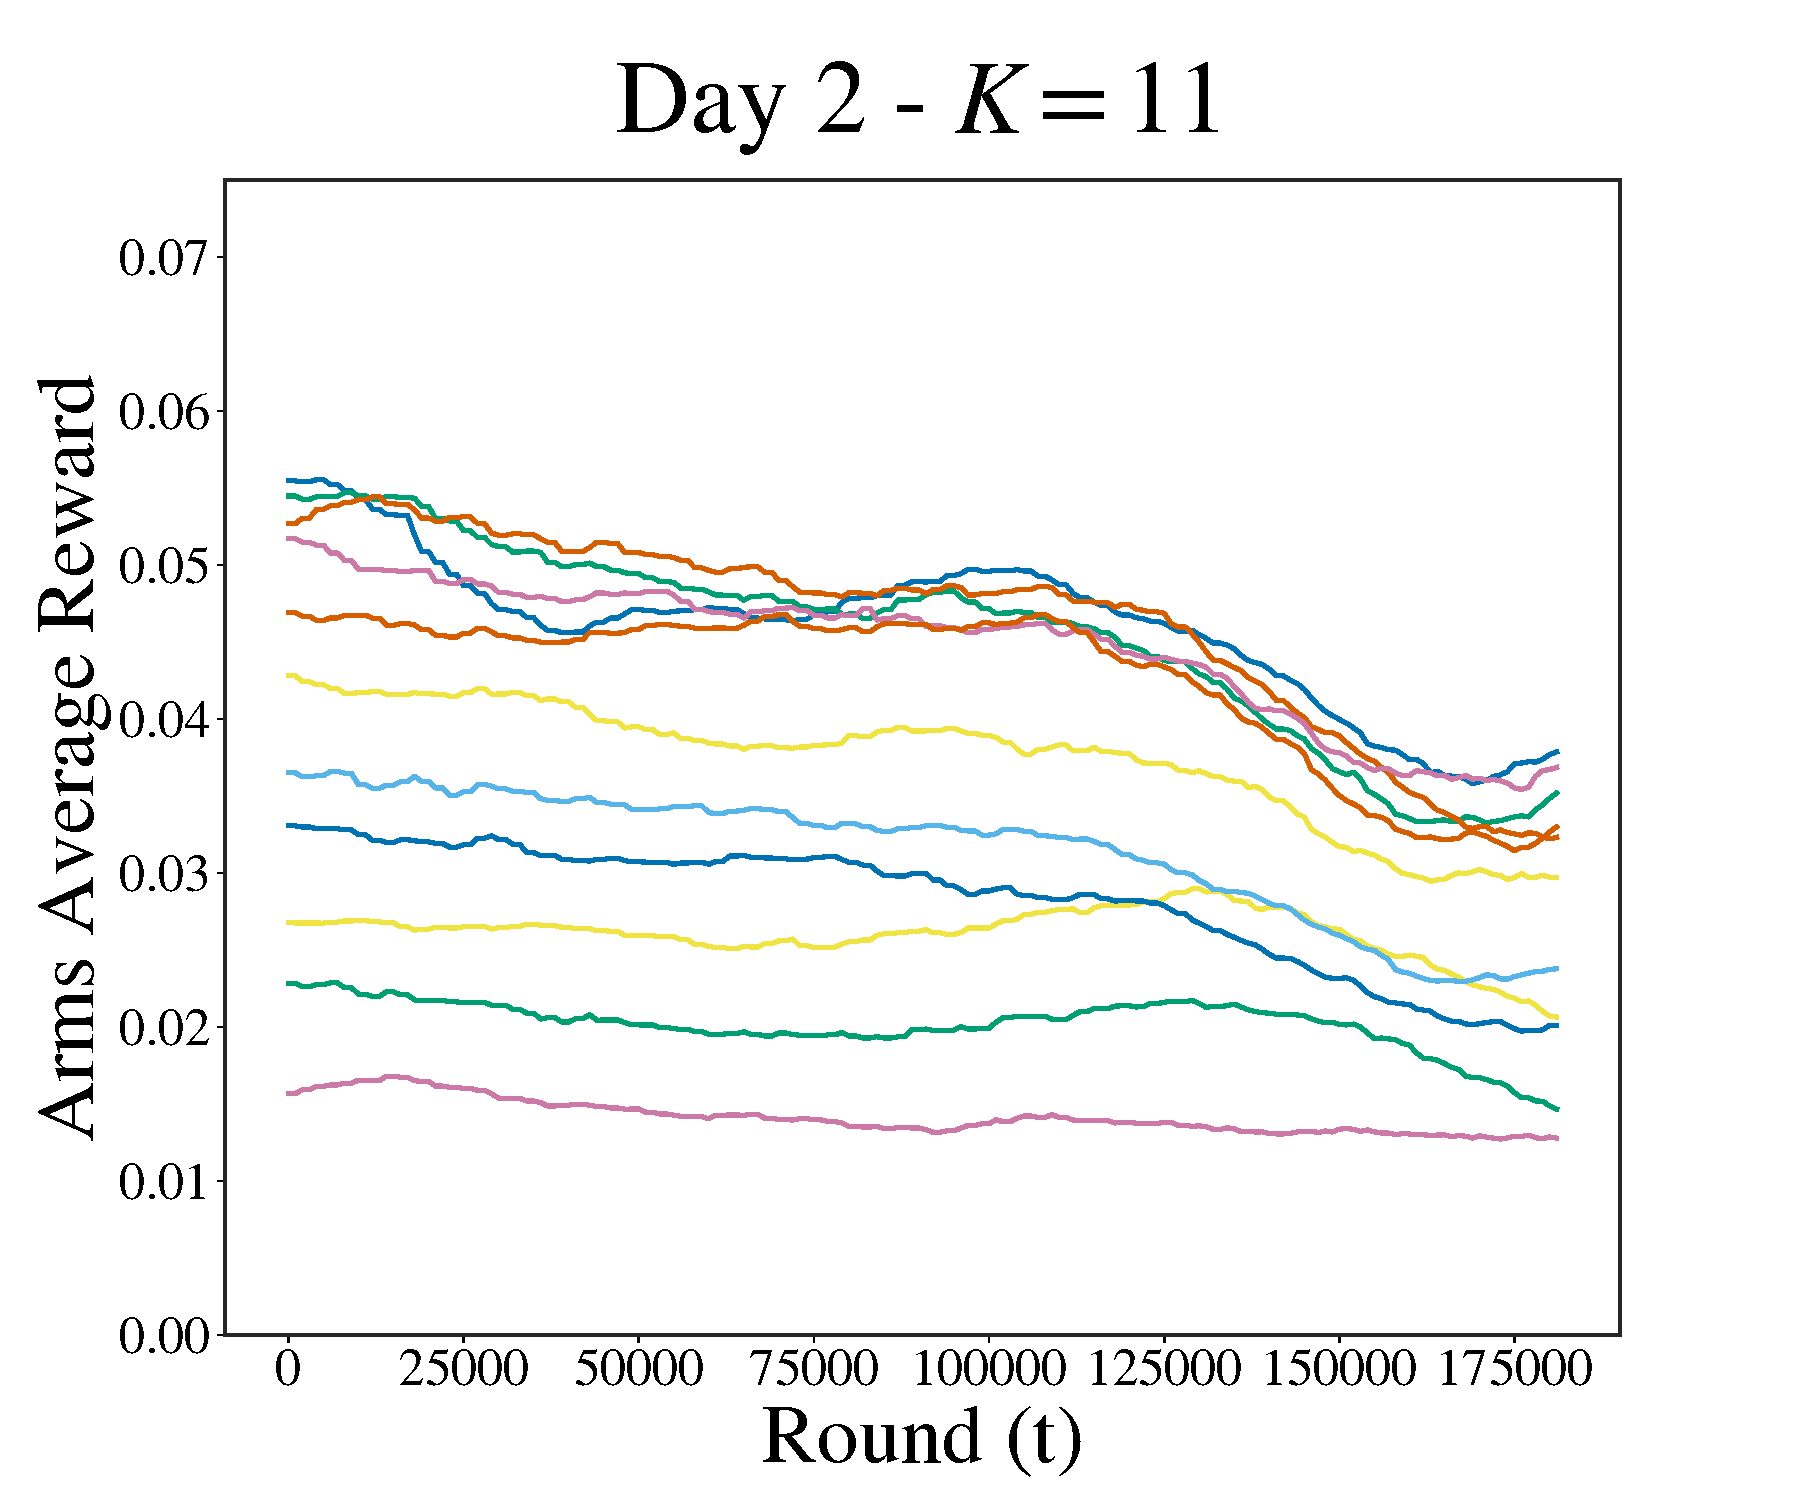
\includegraphics[clip, width= 0.495\textwidth]{4Restless/fig/reward_plot_day2.pdf}
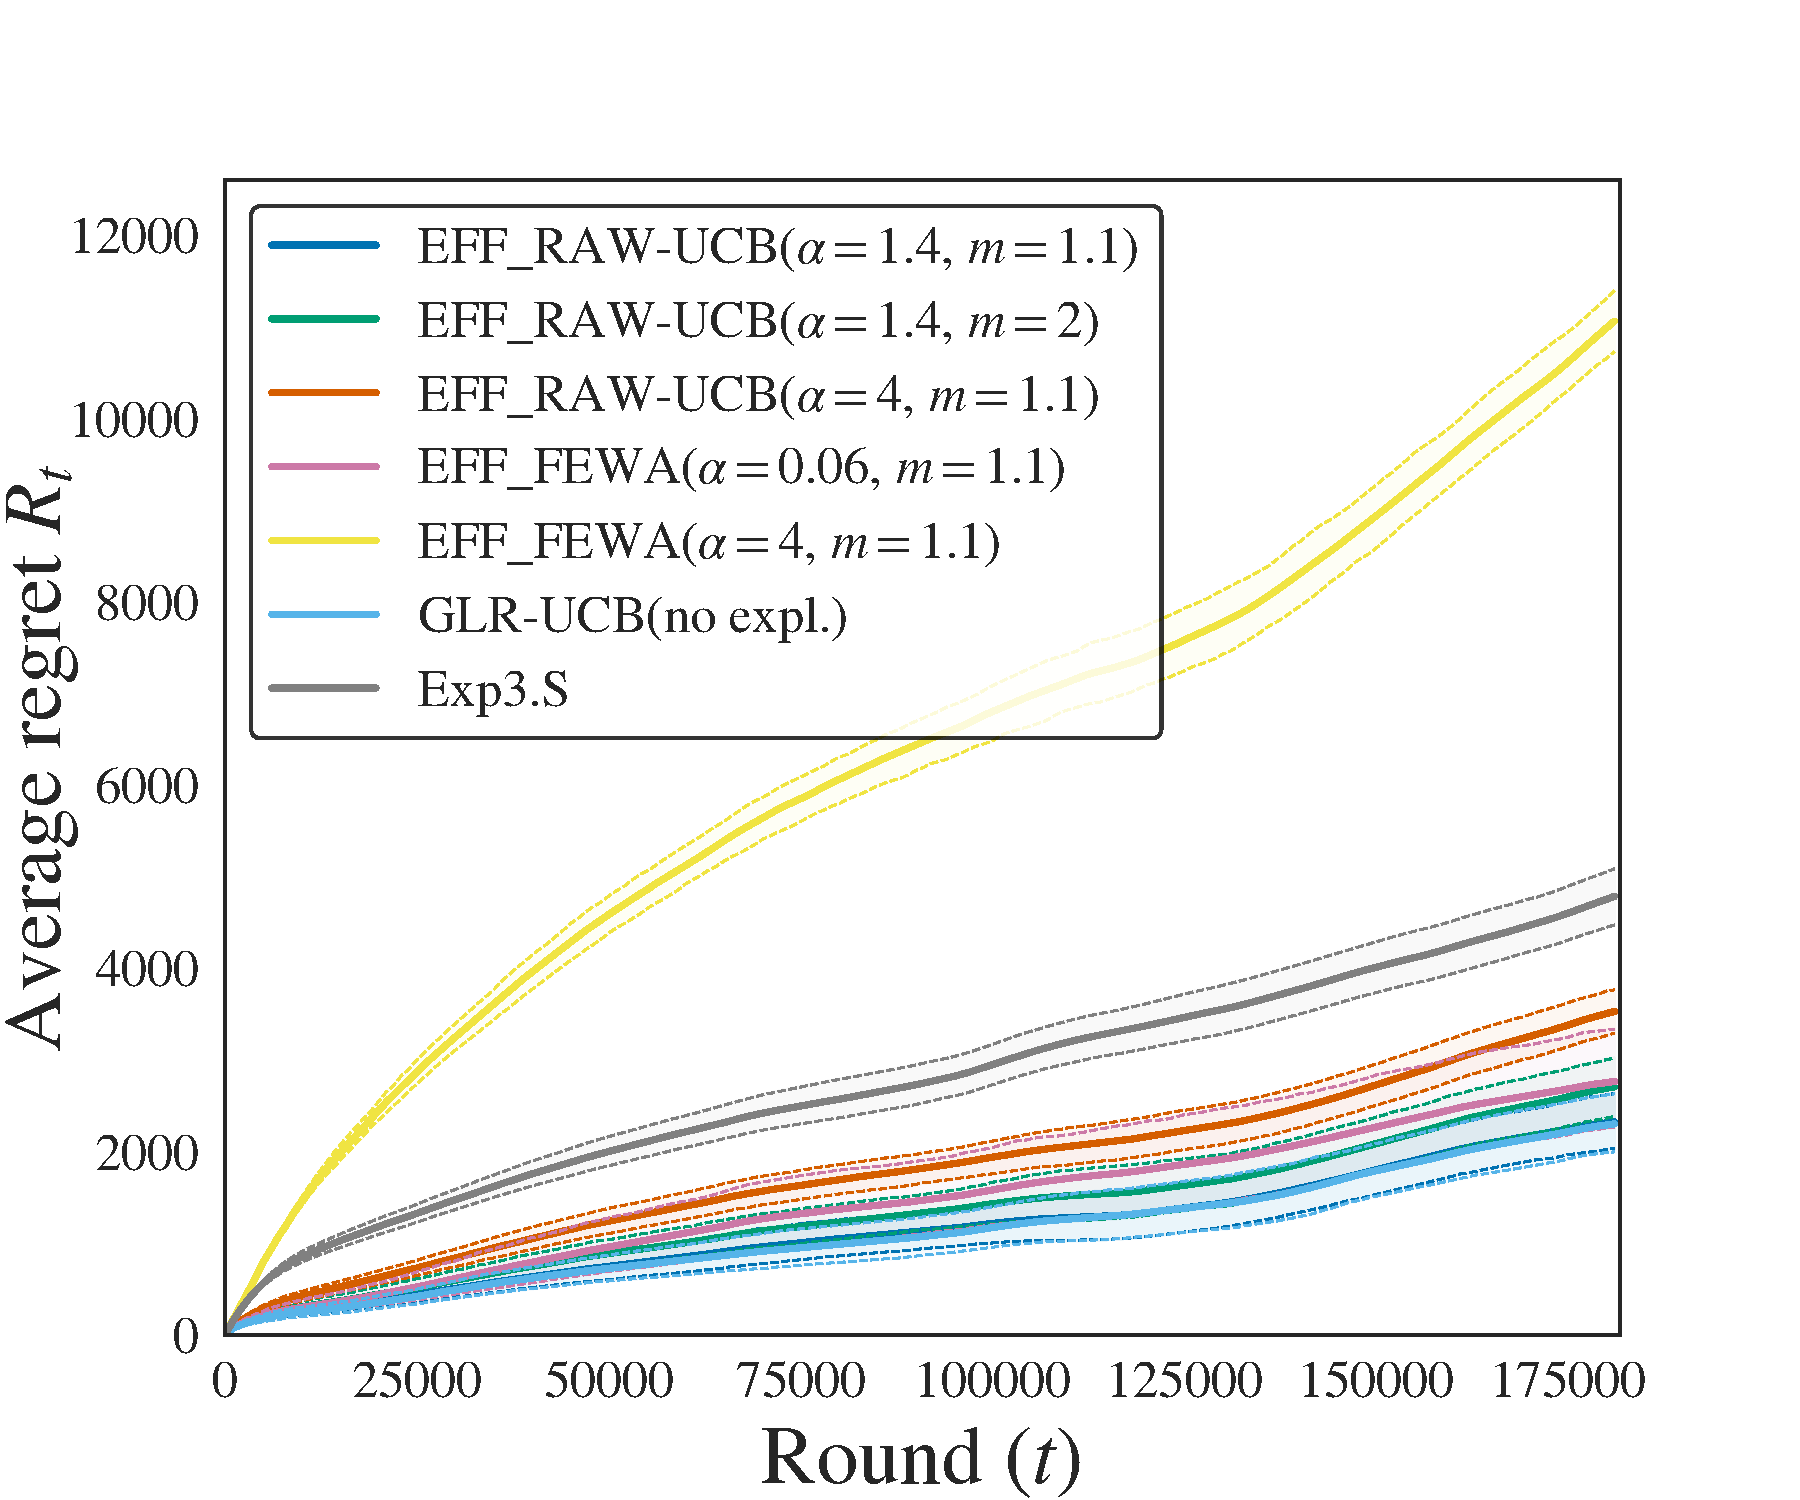
\includegraphics[clip, width= 0.495\textwidth]{4Restless/fig/DAY2.pdf}
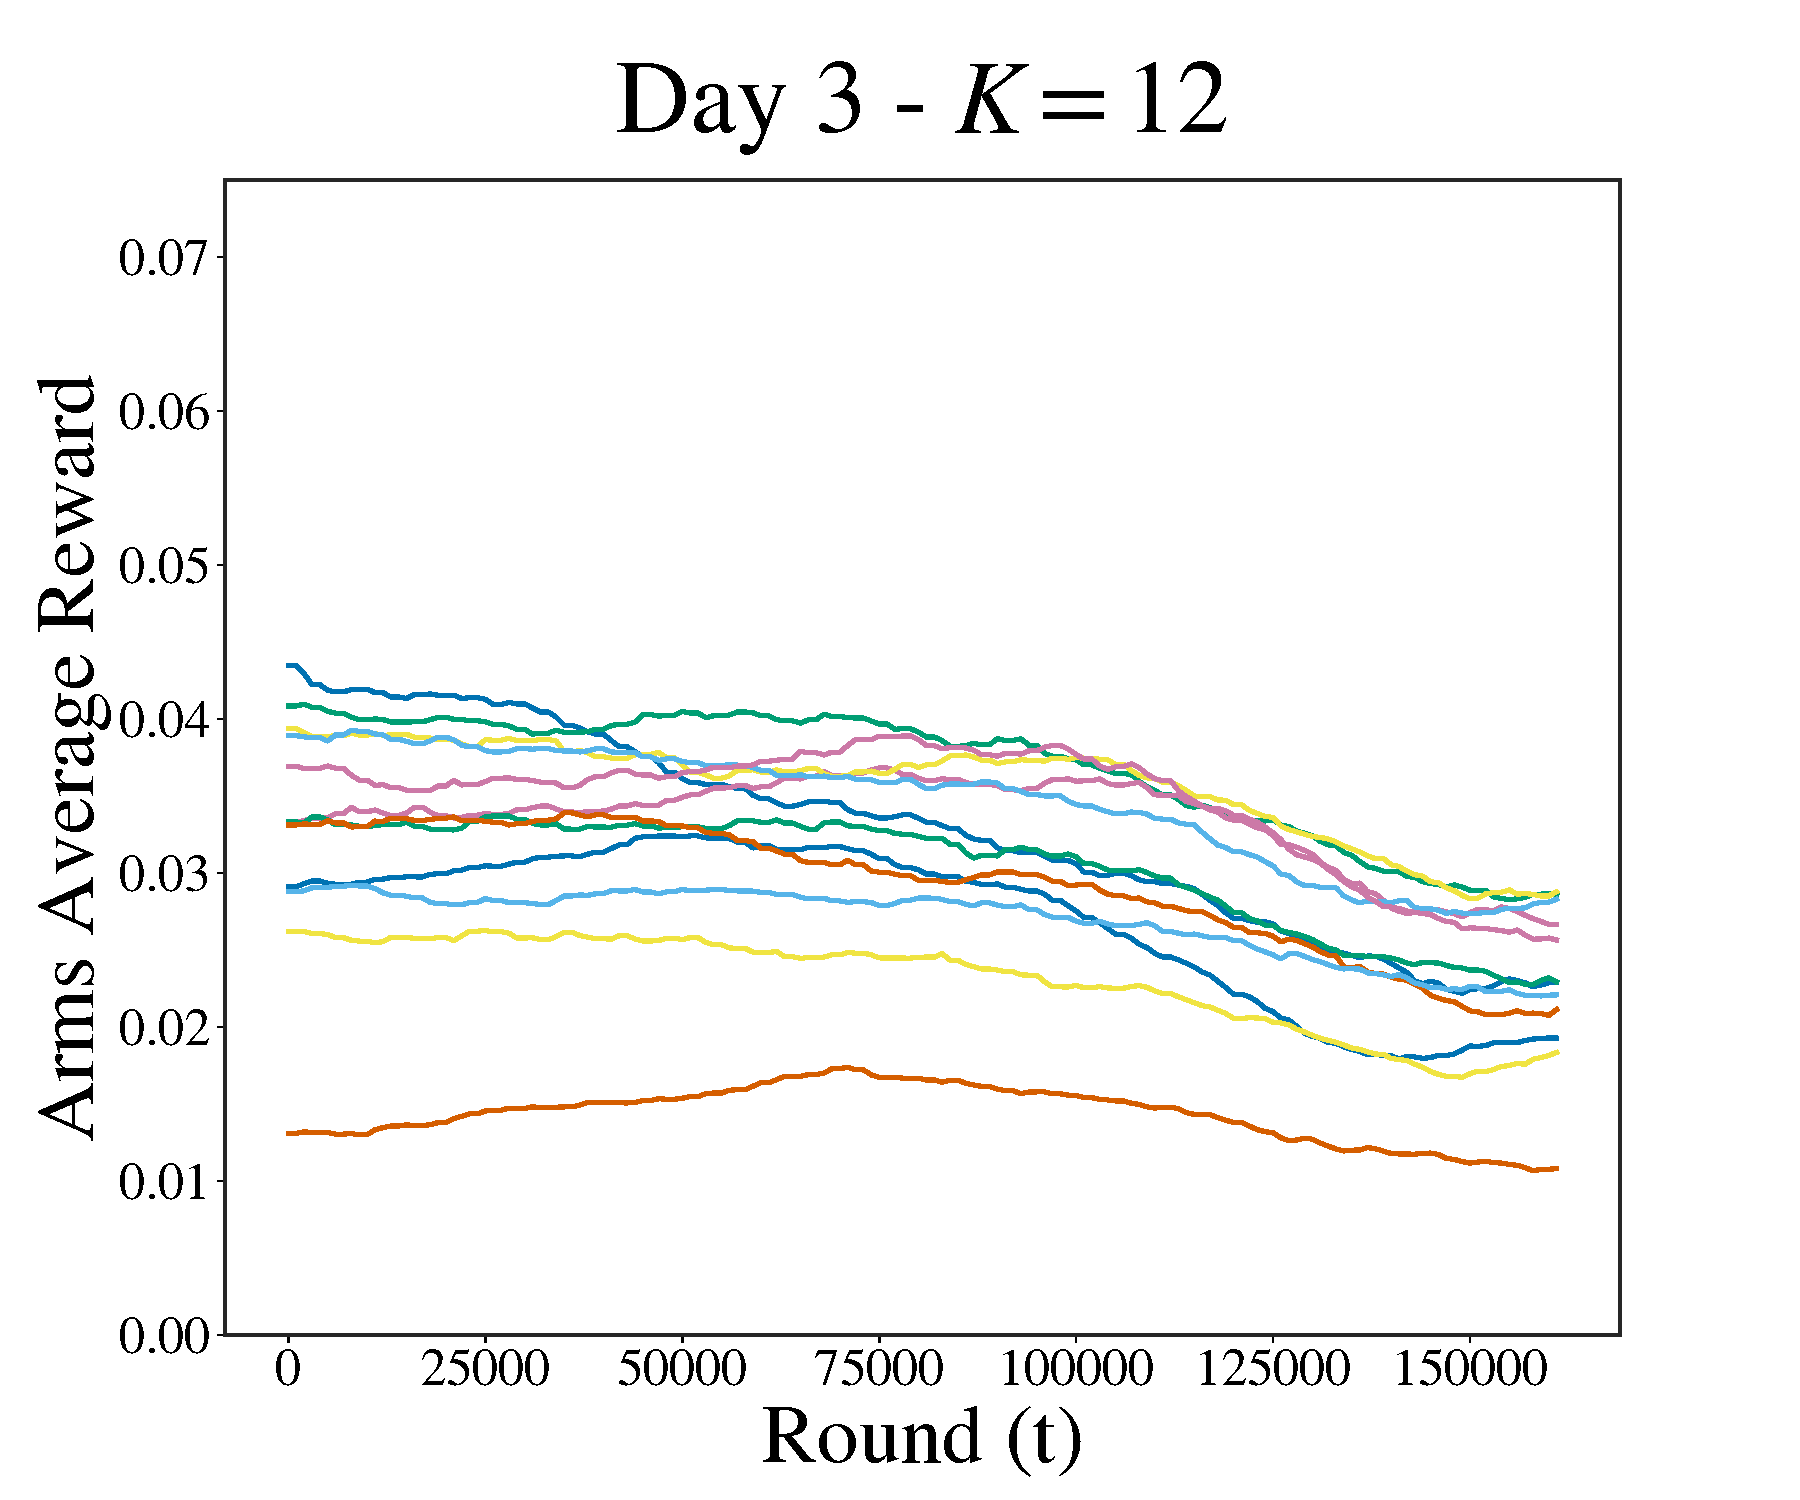
\includegraphics[clip, width= 0.495\textwidth]{4Restless/fig/reward_plot_day3.pdf}
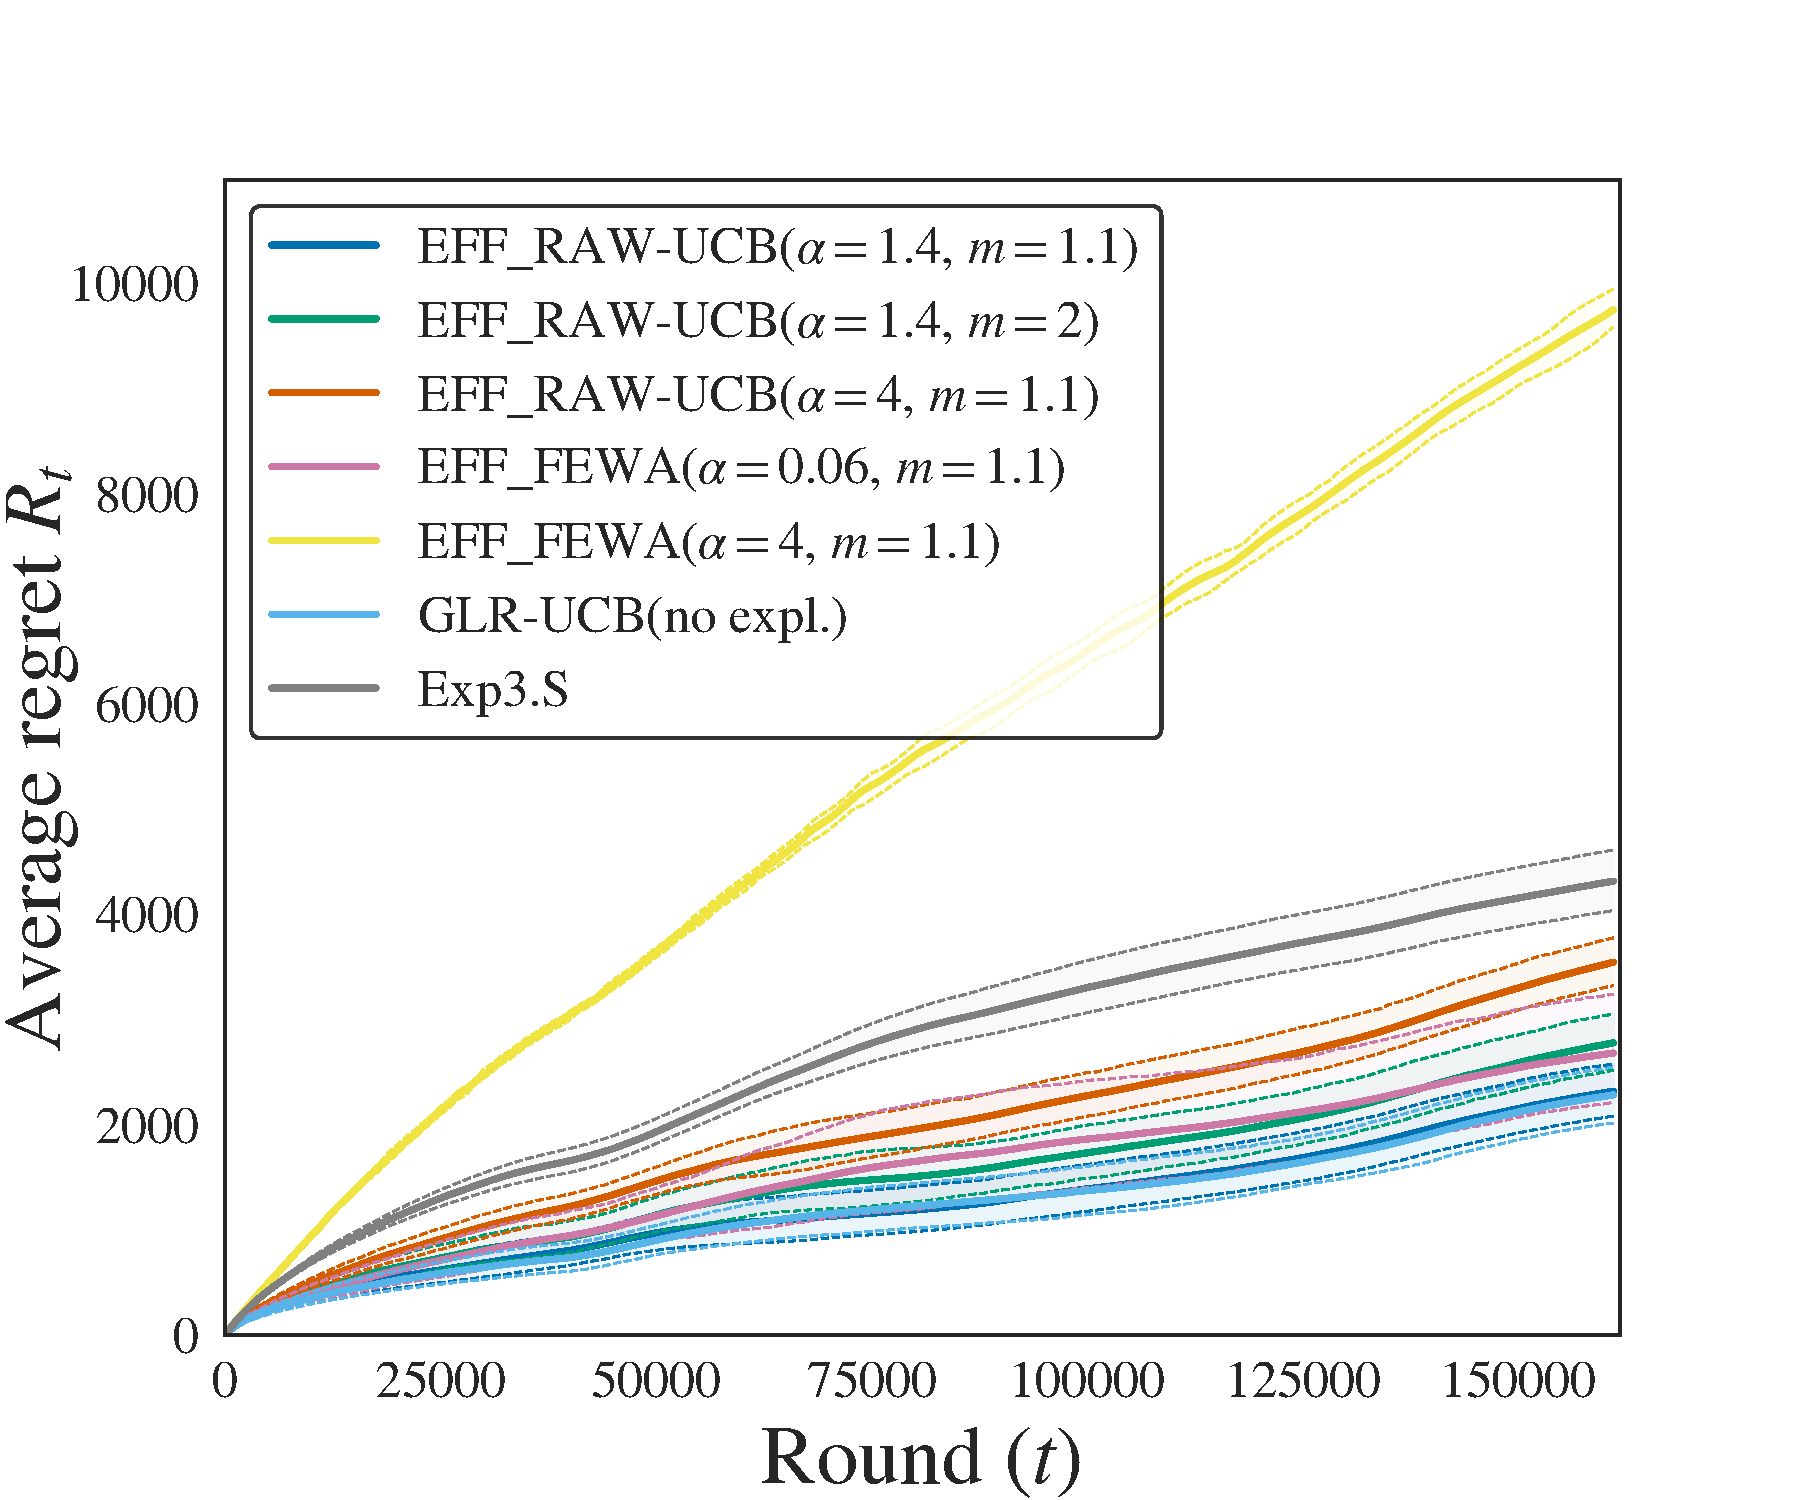
\includegraphics[clip, width= 0.495\textwidth]{4Restless/fig/DAY3.pdf}
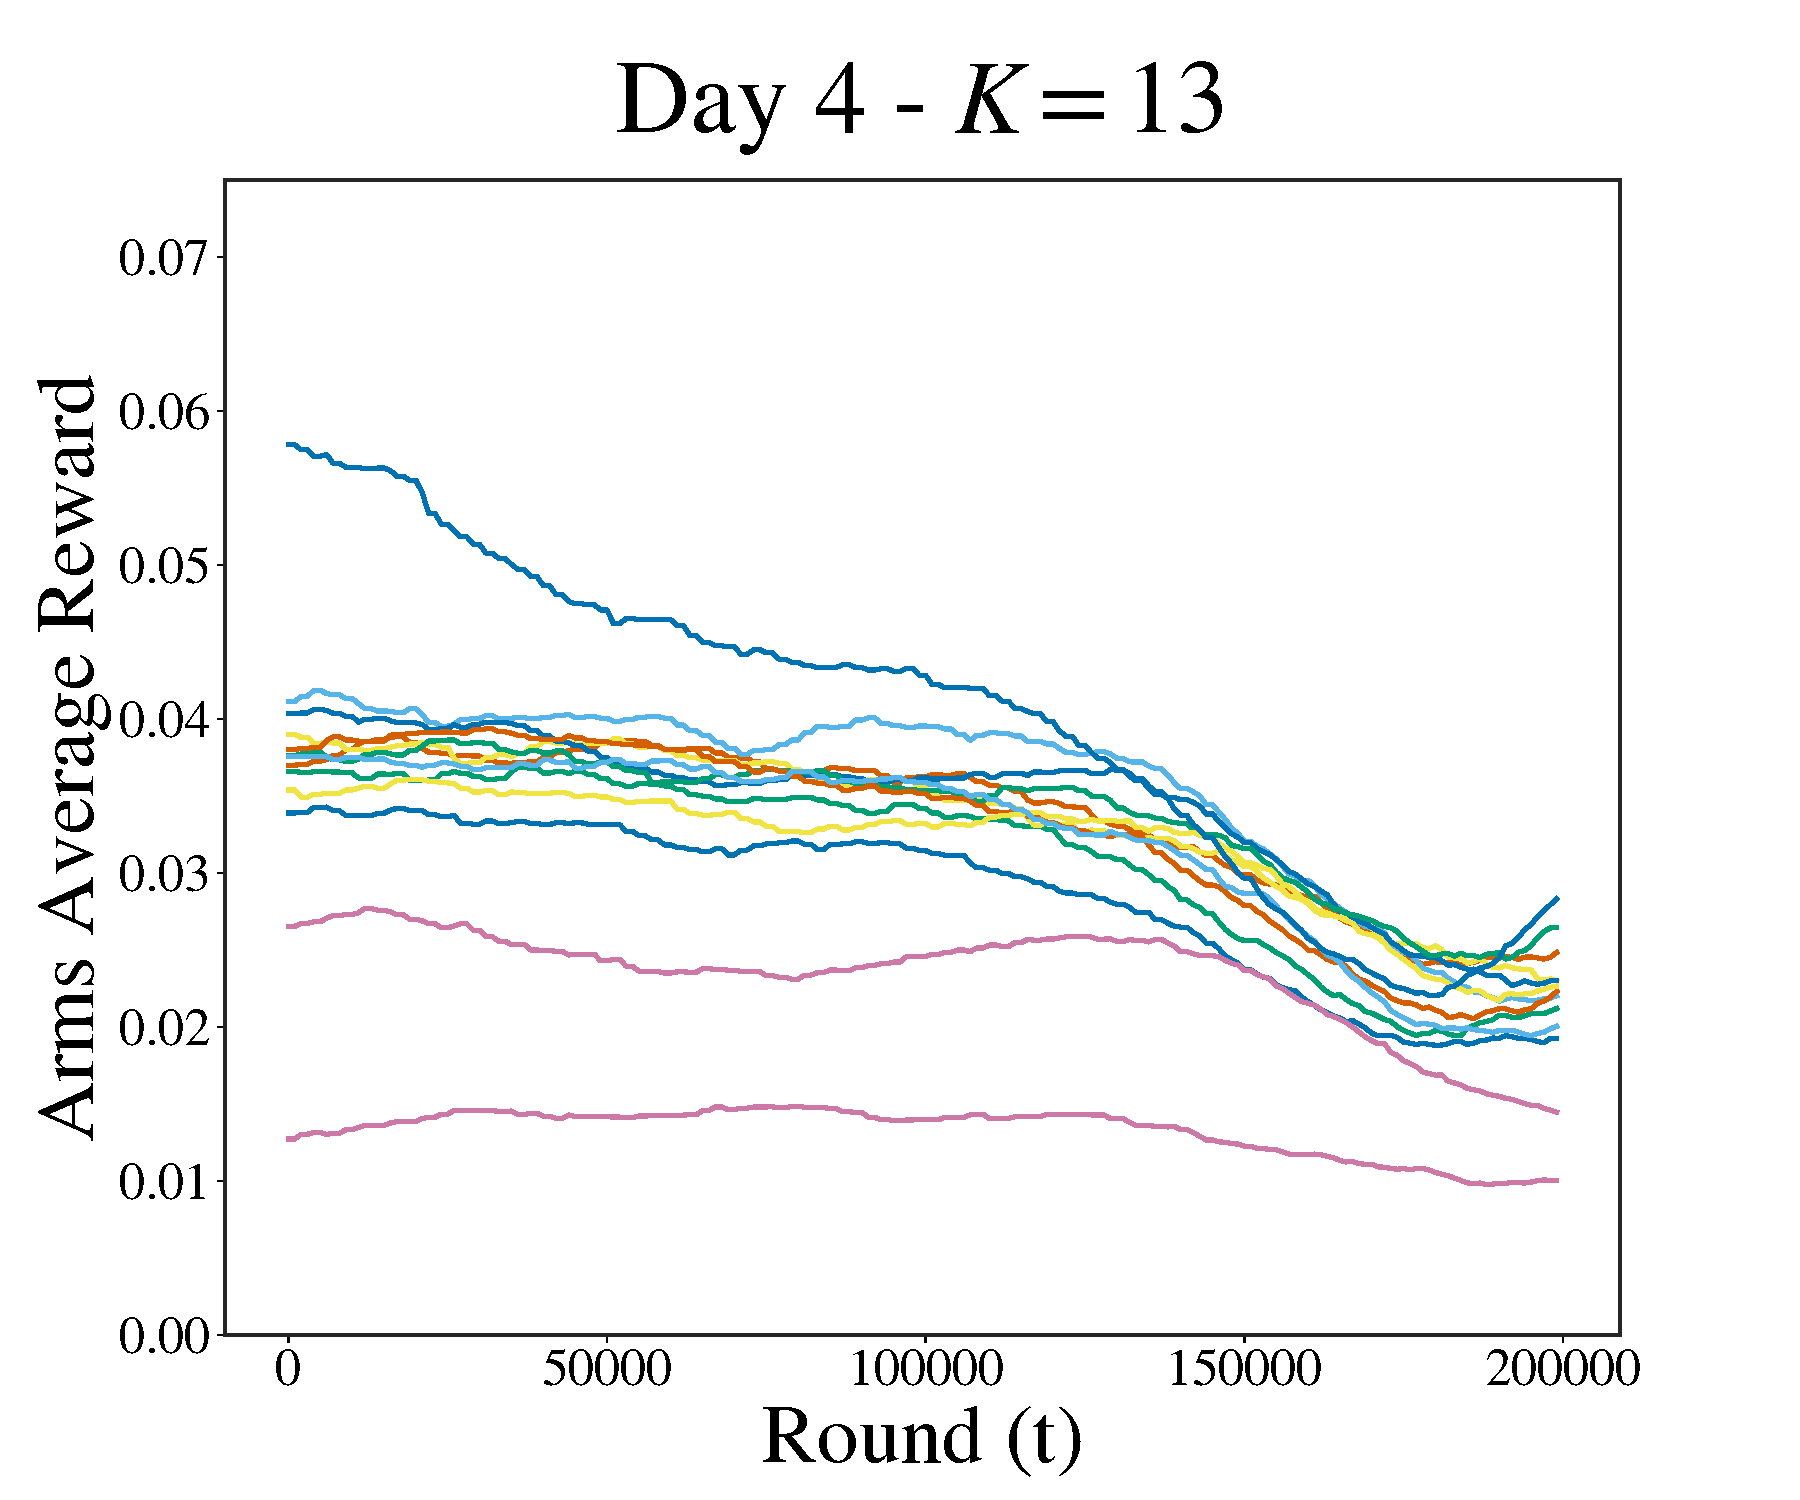
\includegraphics[clip, width= 0.495\textwidth]{4Restless/fig/reward_plot_day4.pdf}
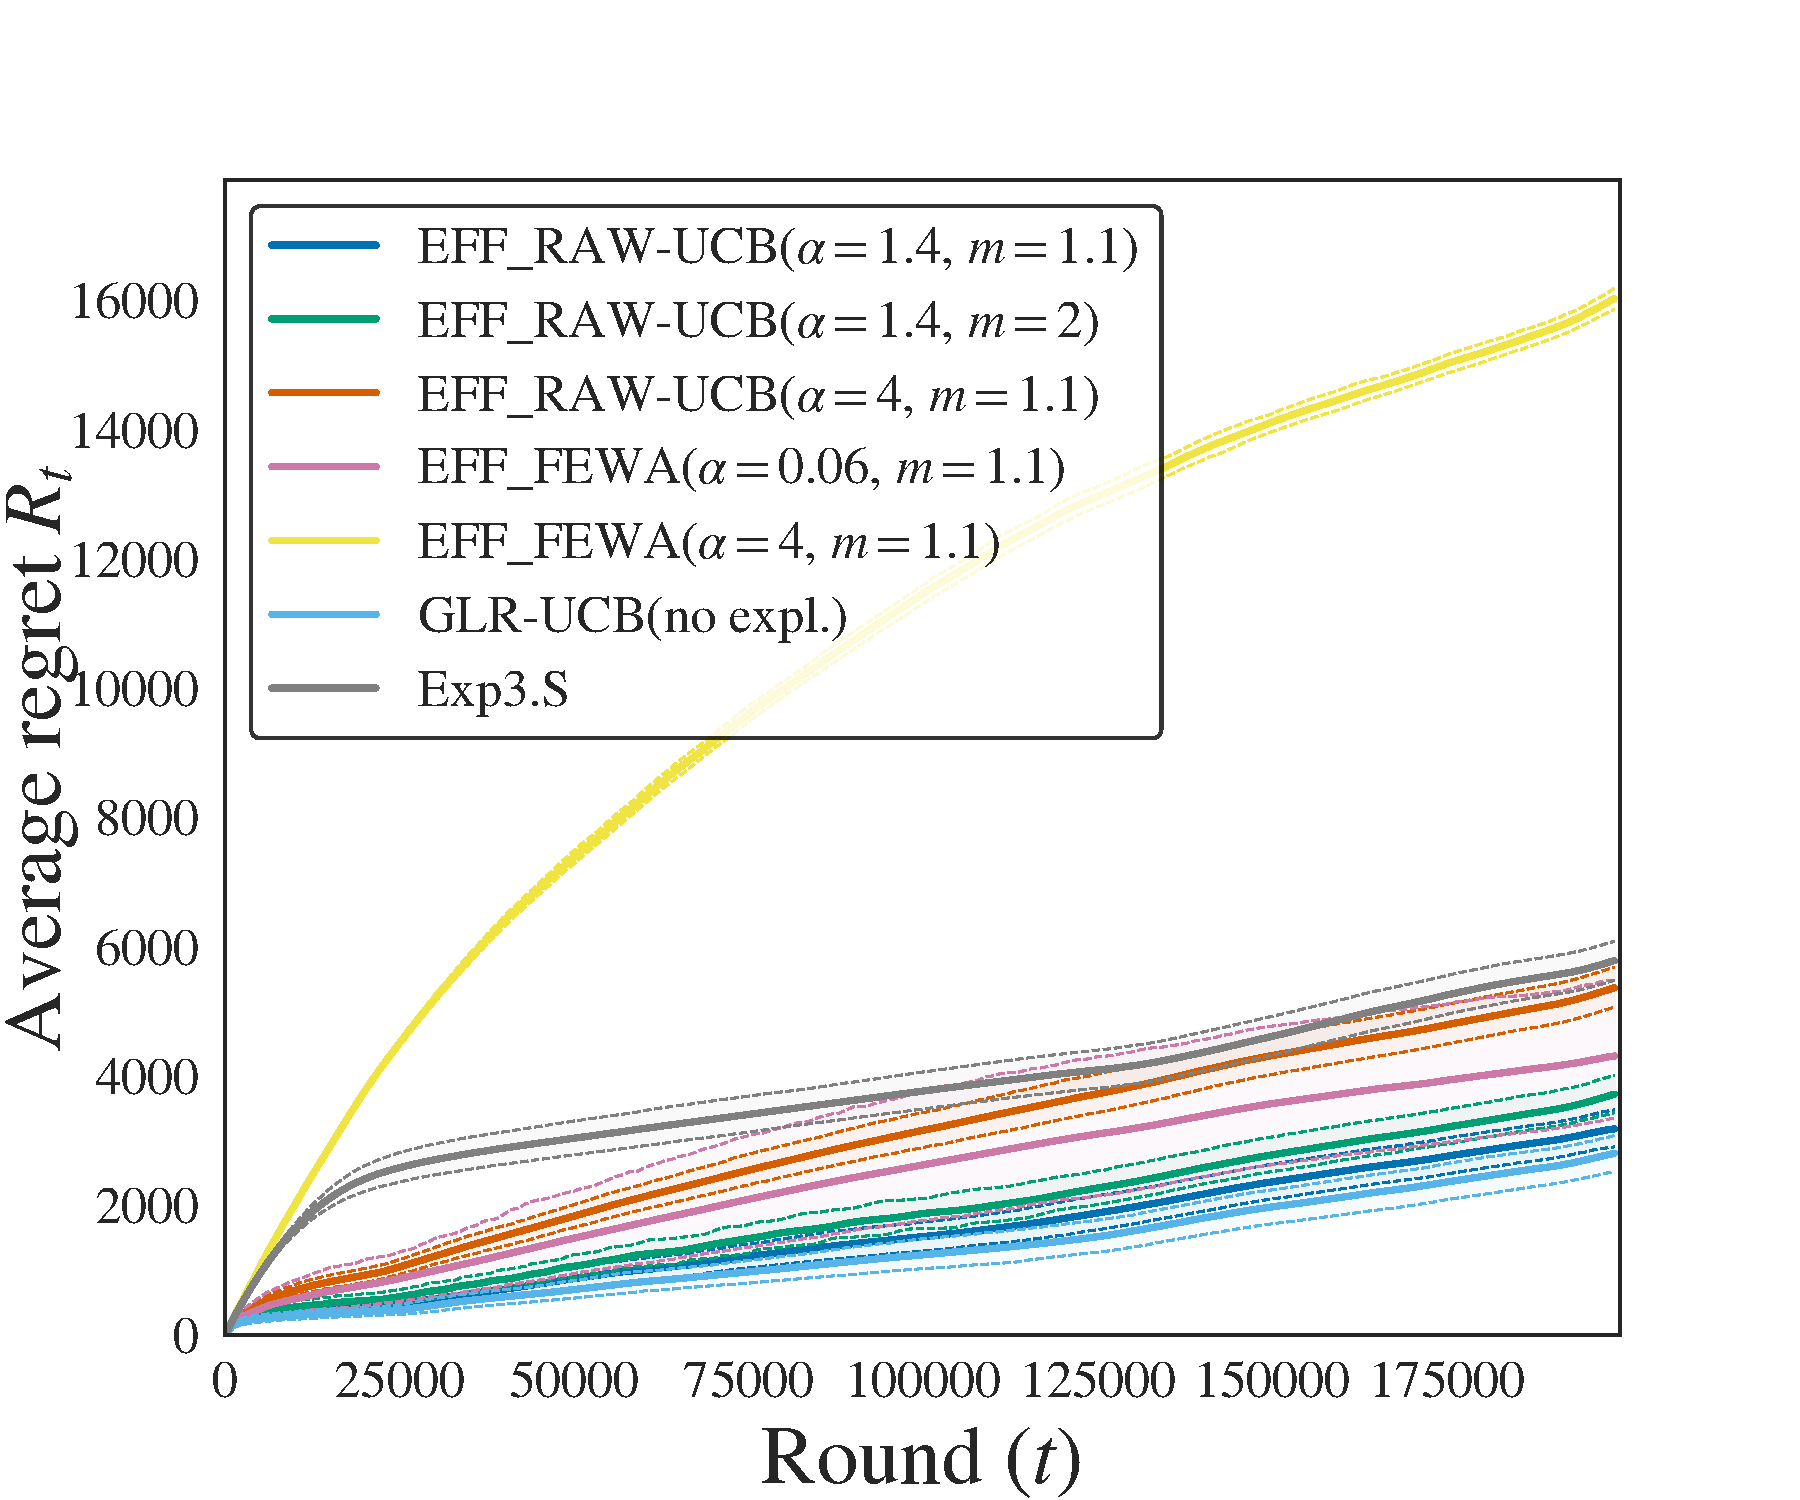
\includegraphics[clip, width= 0.495\textwidth]{4Restless/fig/DAY4.pdf}
\end{figure*}

\begin{figure*}[p!]
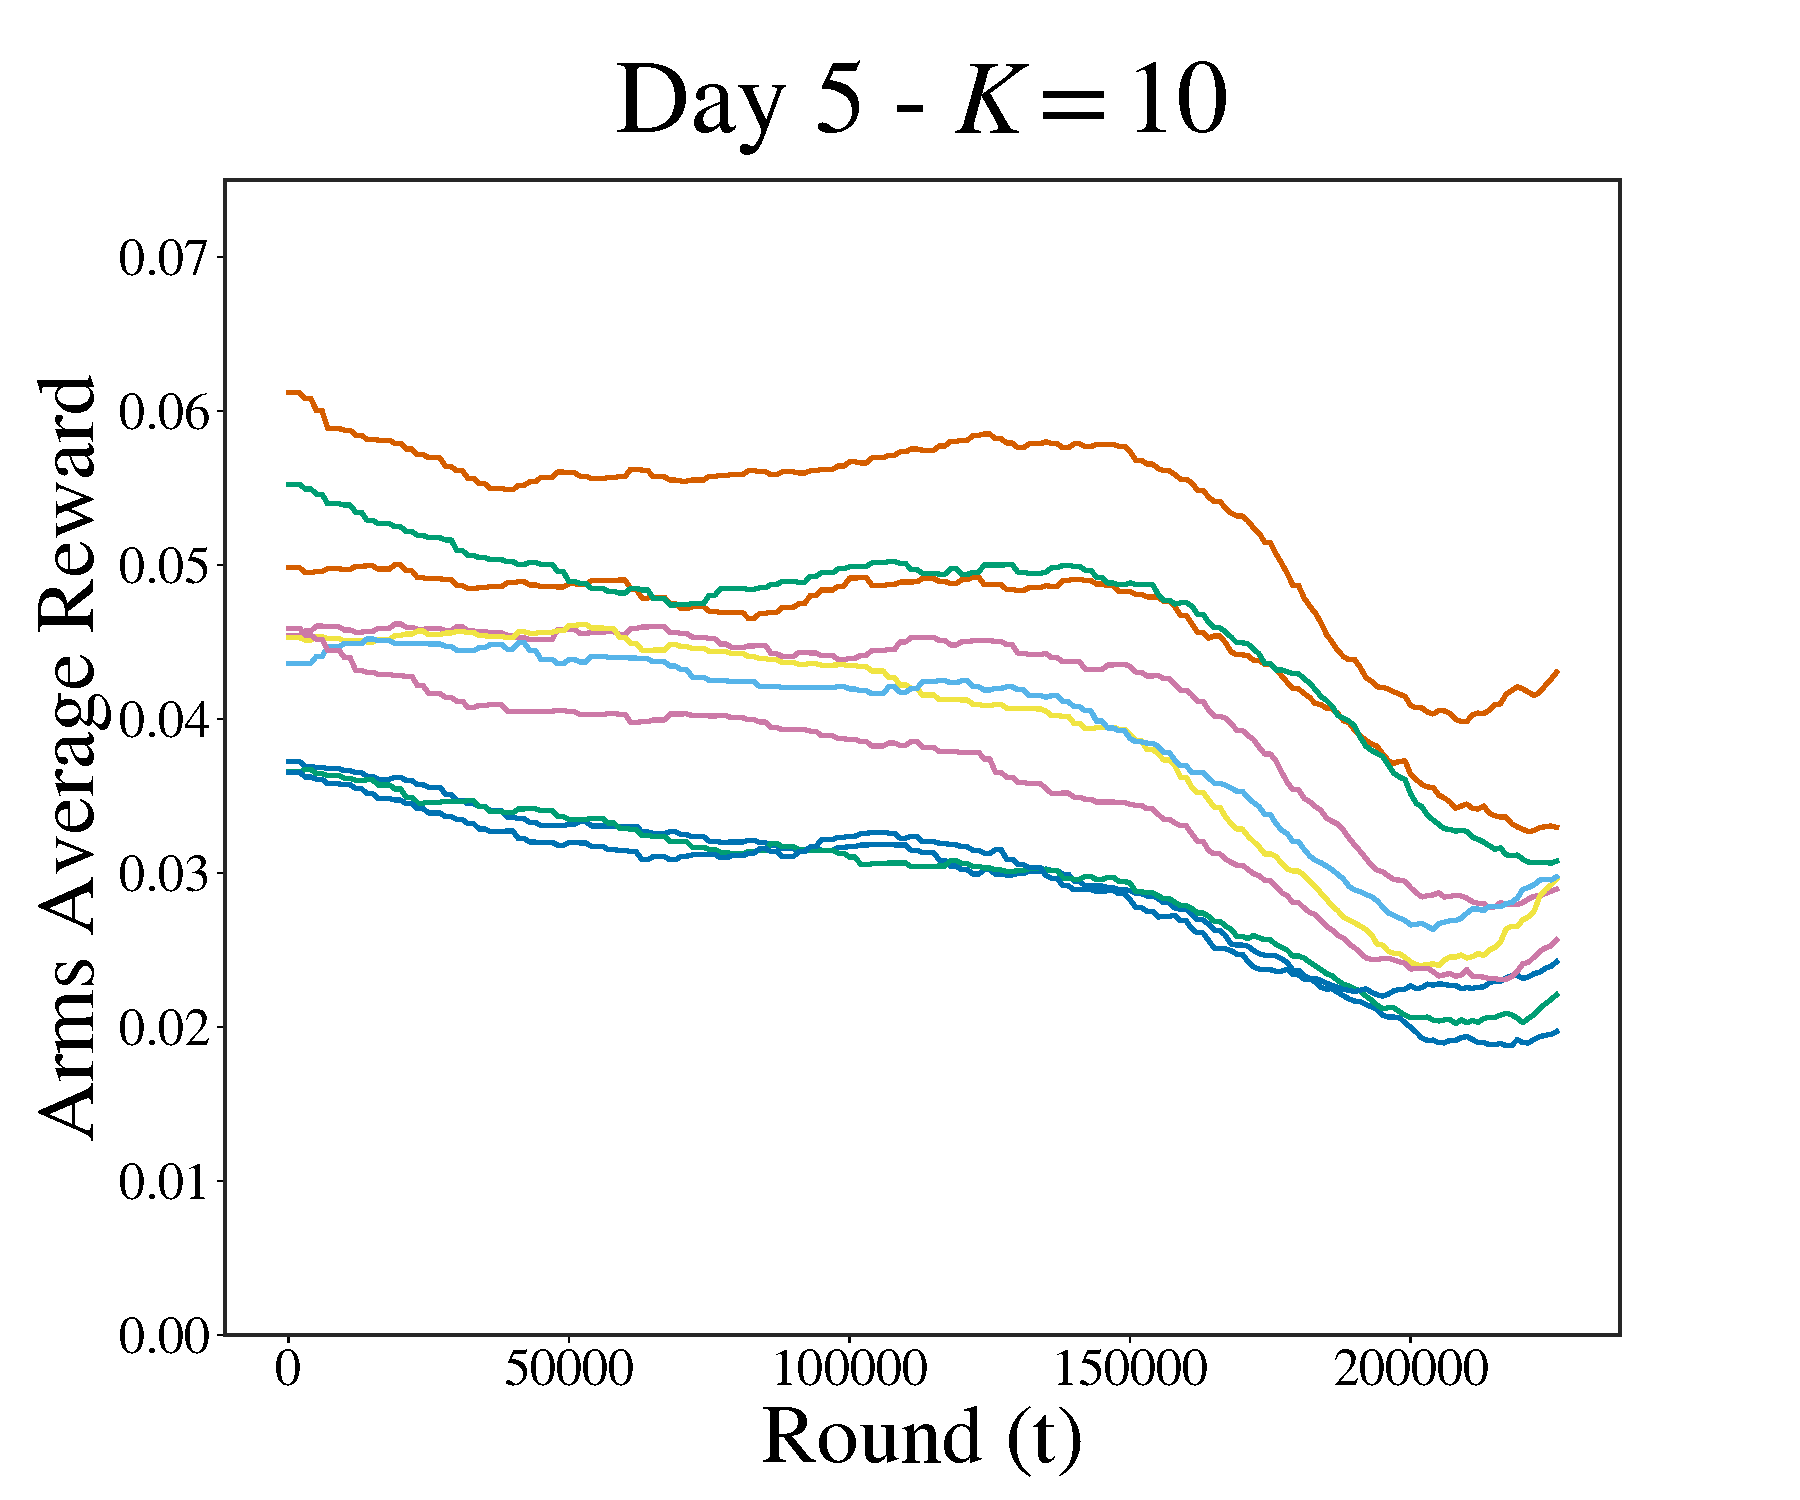
\includegraphics[clip, width= 0.495\textwidth]{4Restless/fig/reward_plot_day5.pdf}
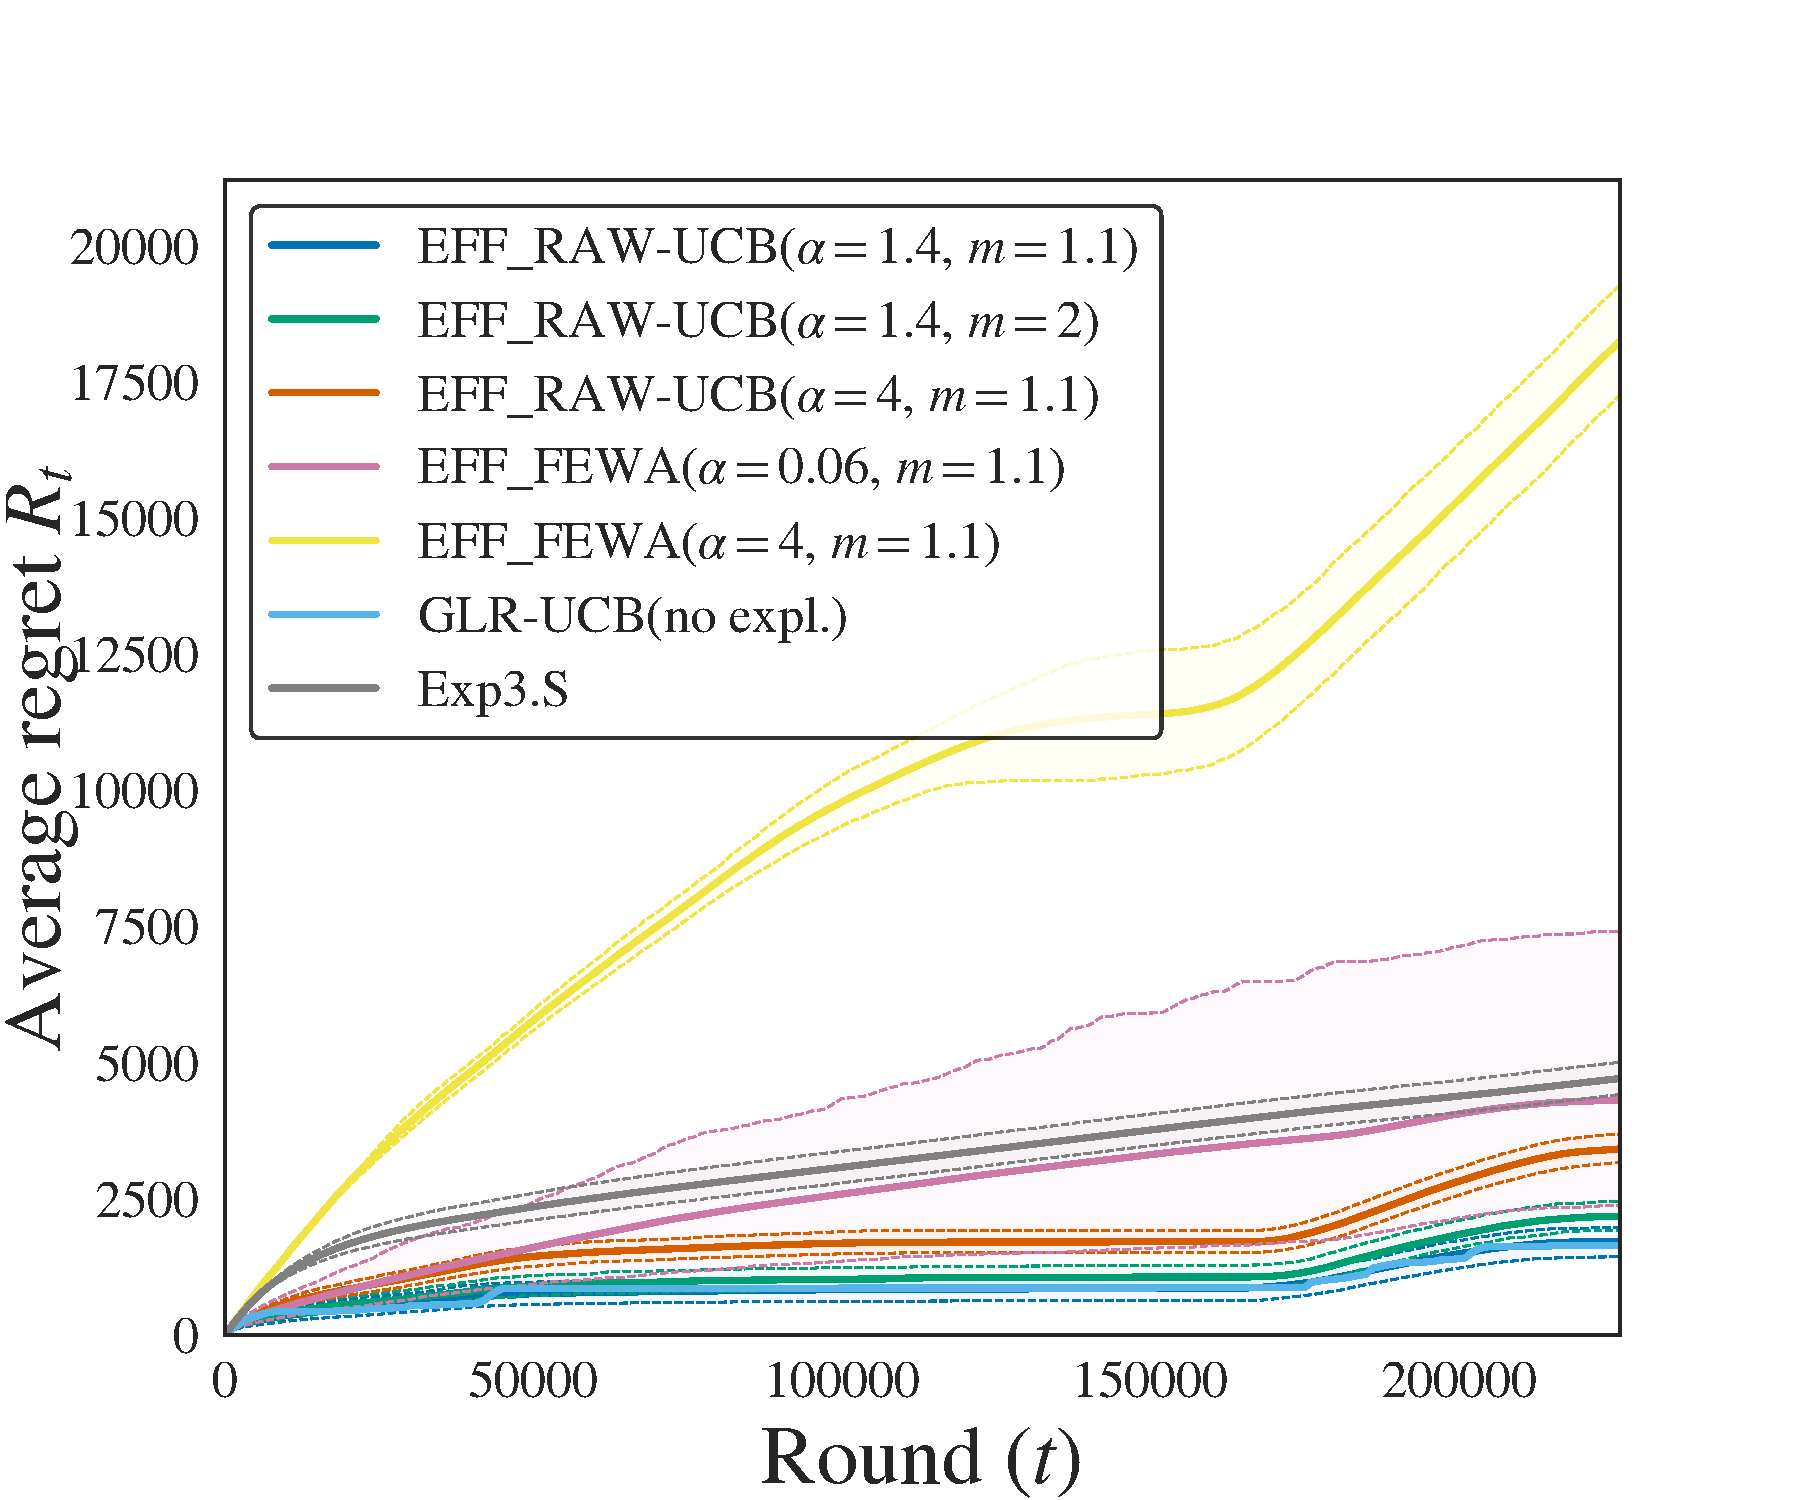
\includegraphics[clip, width= 0.495\textwidth]{4Restless/fig/DAY5.pdf}
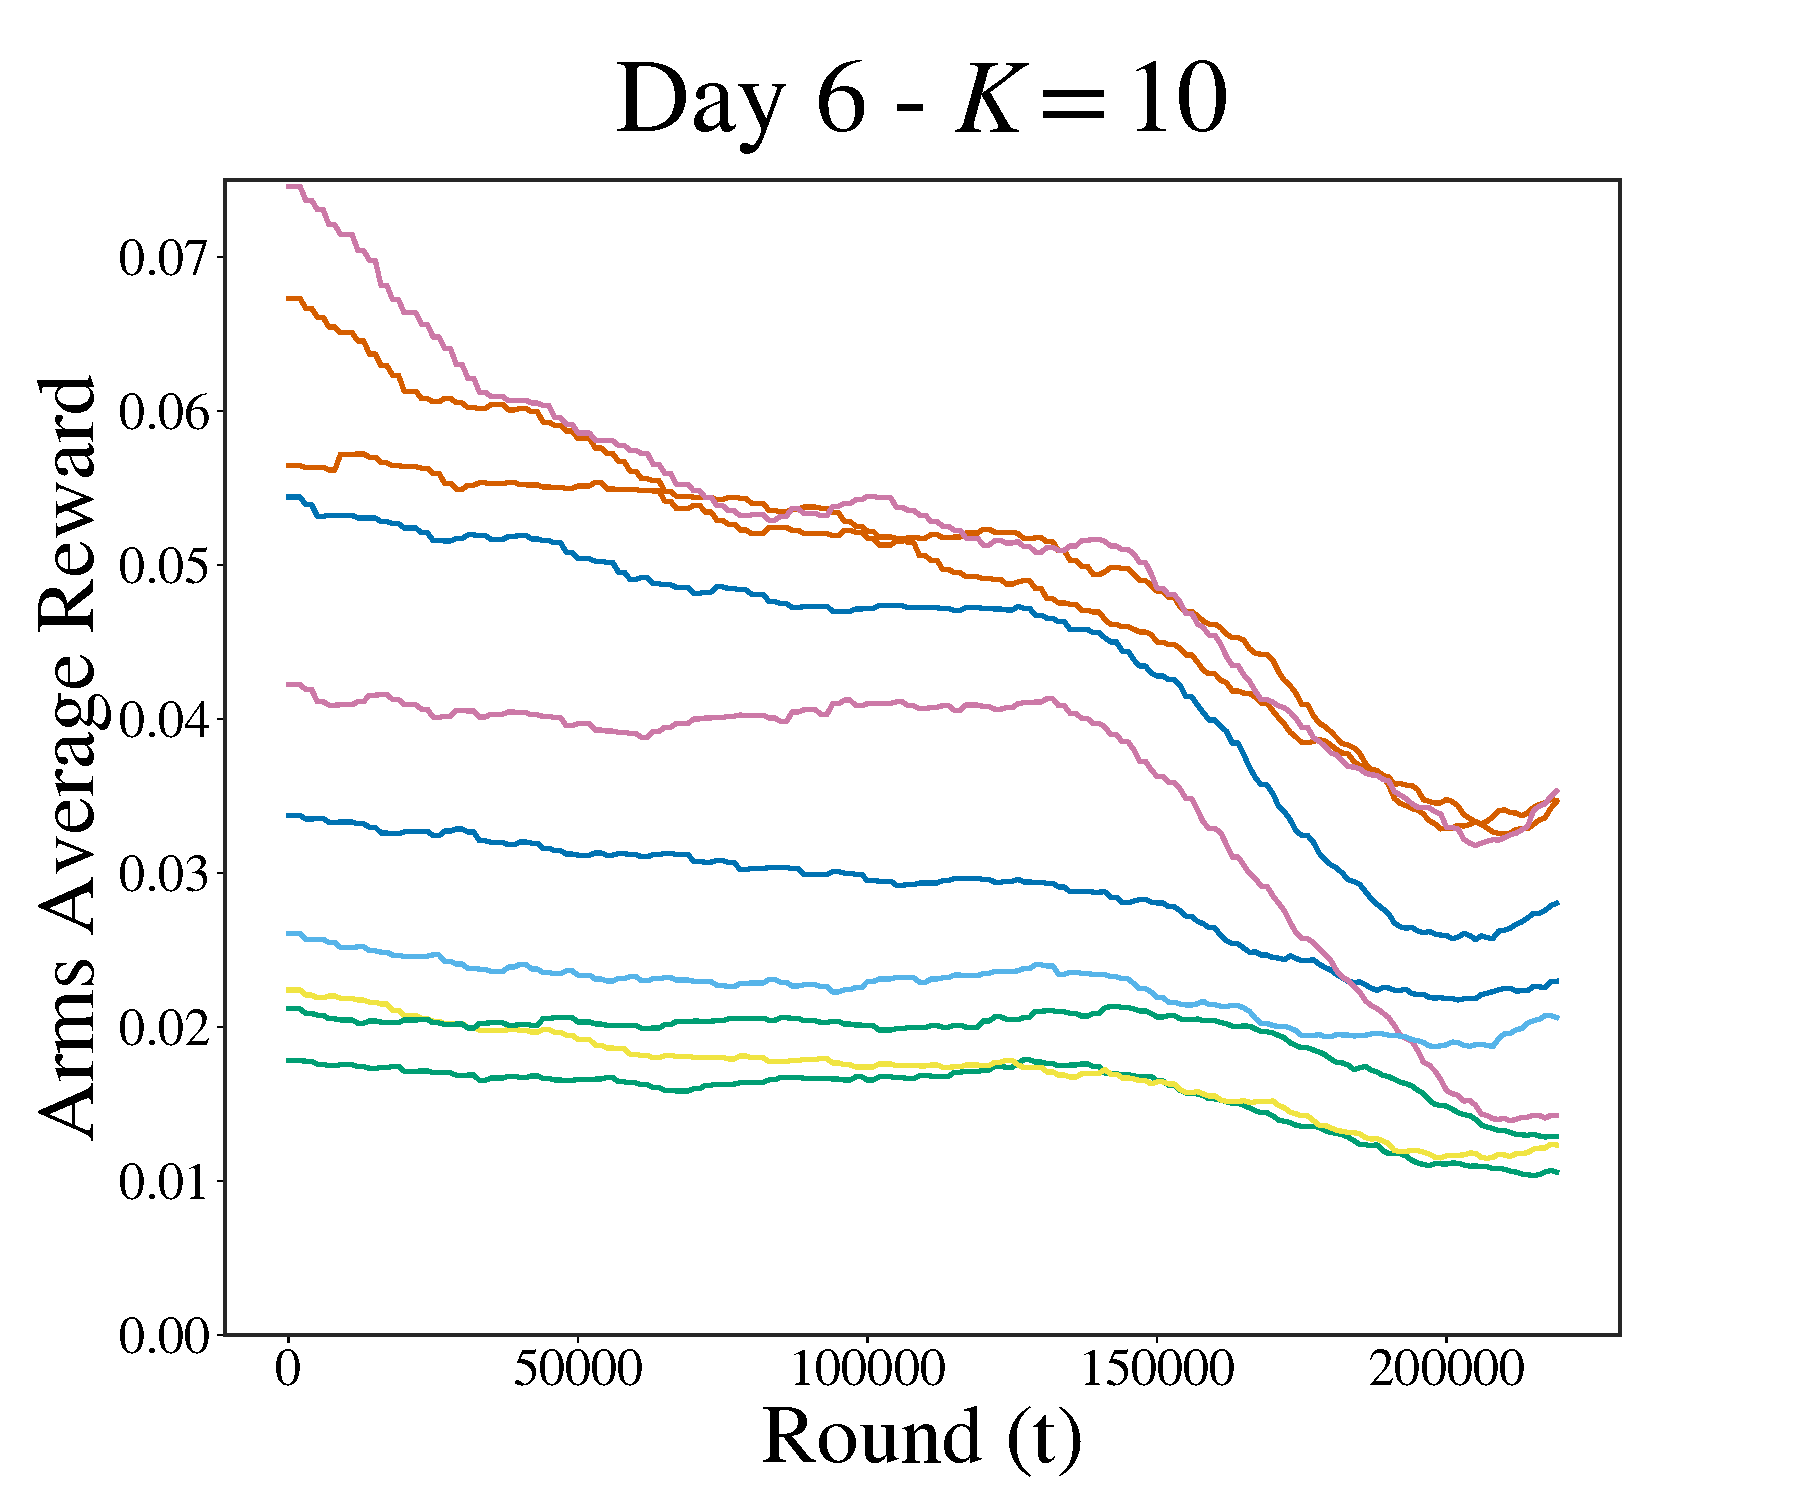
\includegraphics[clip, width= 0.495\textwidth]{4Restless/fig/reward_plot_day6.pdf}
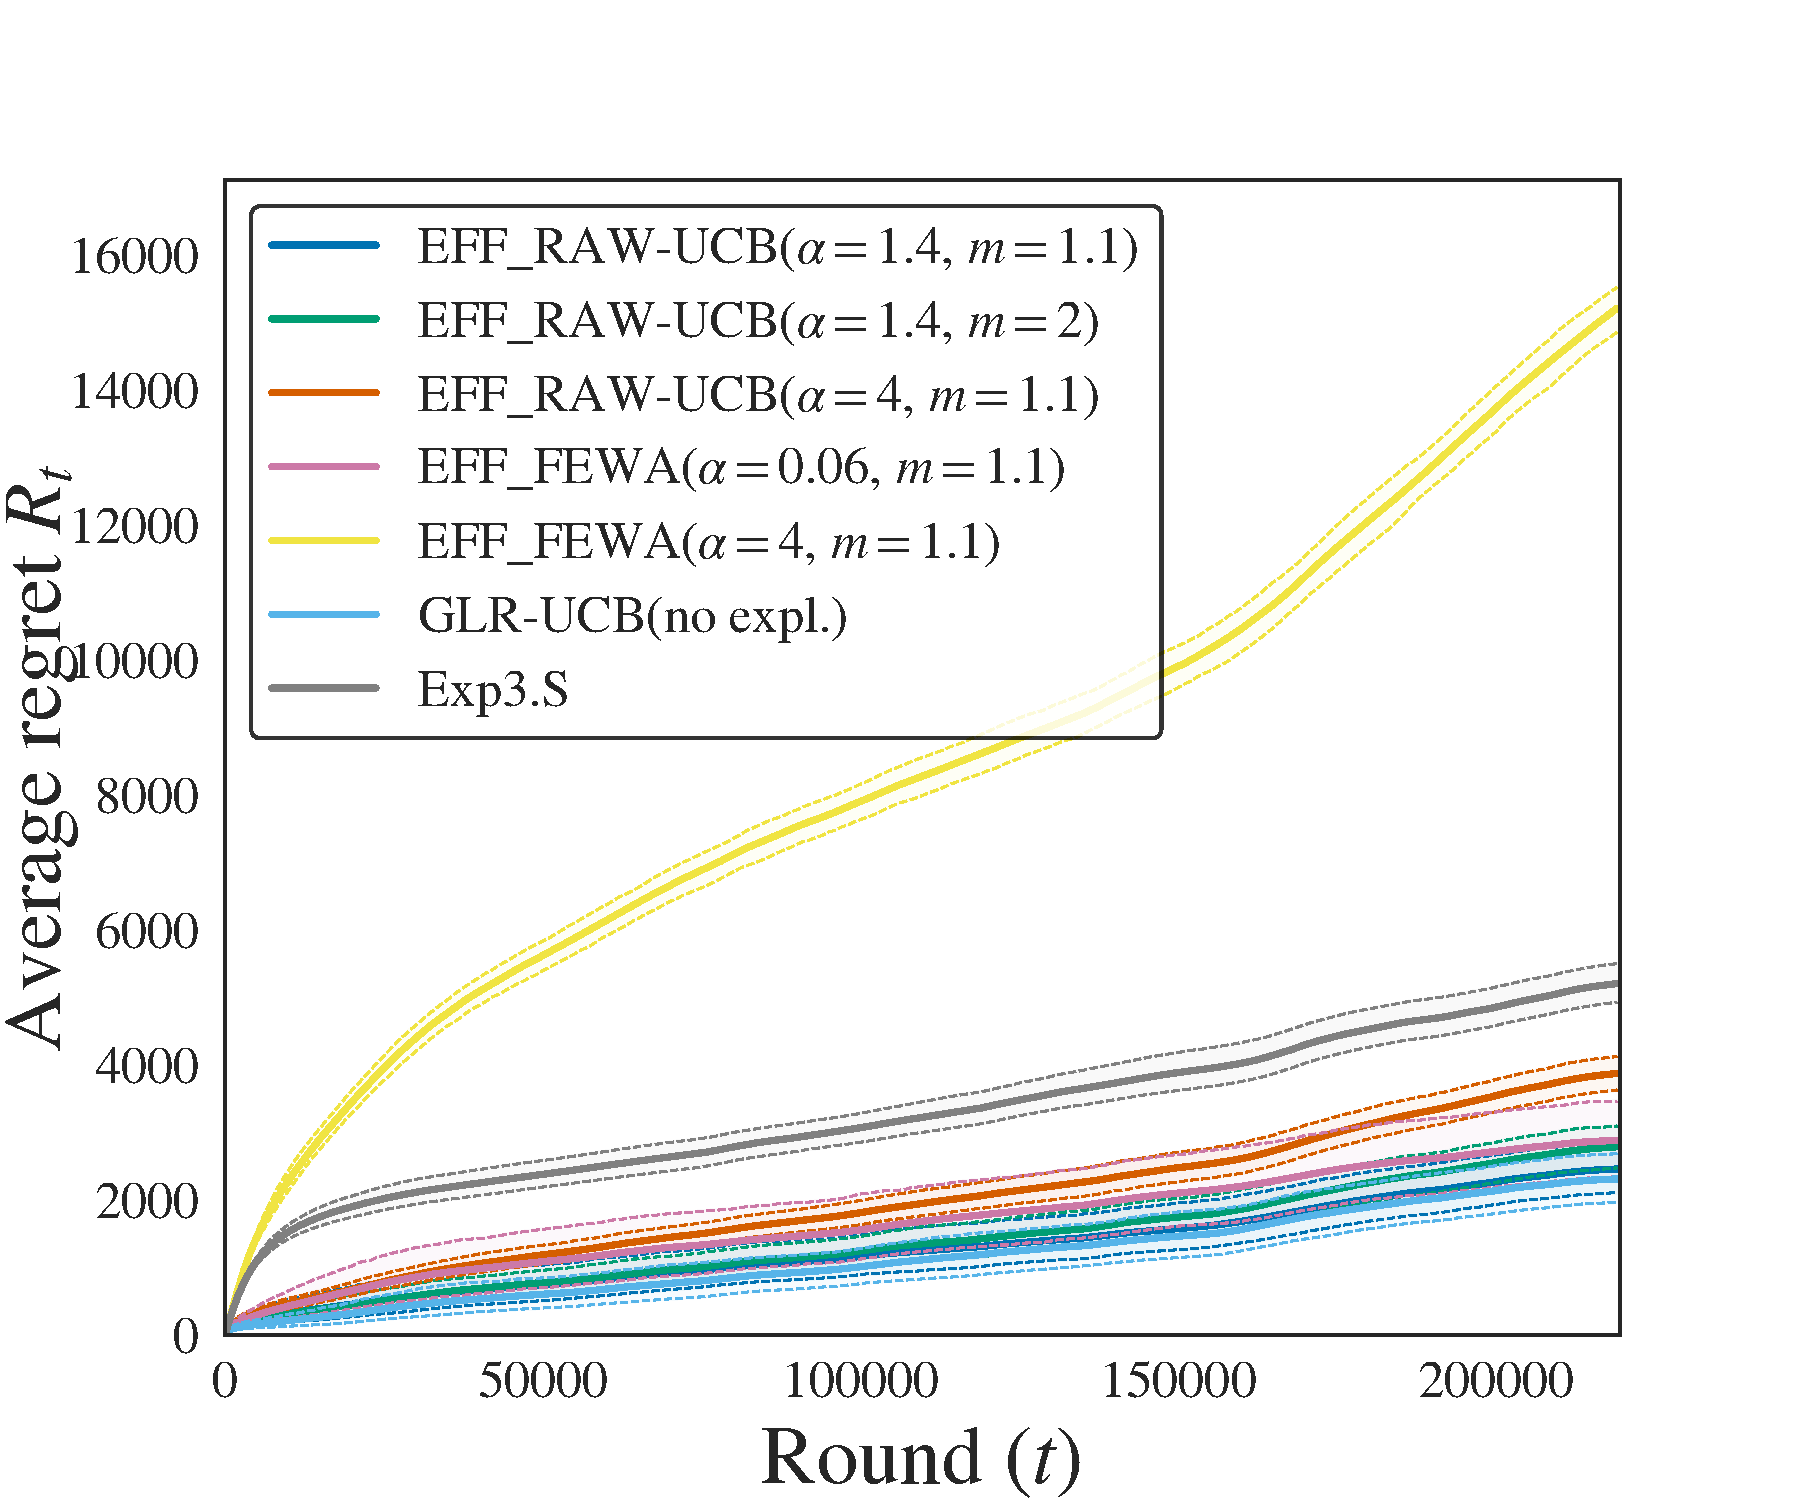
\includegraphics[clip, width= 0.495\textwidth]{4Restless/fig/DAY6.pdf}
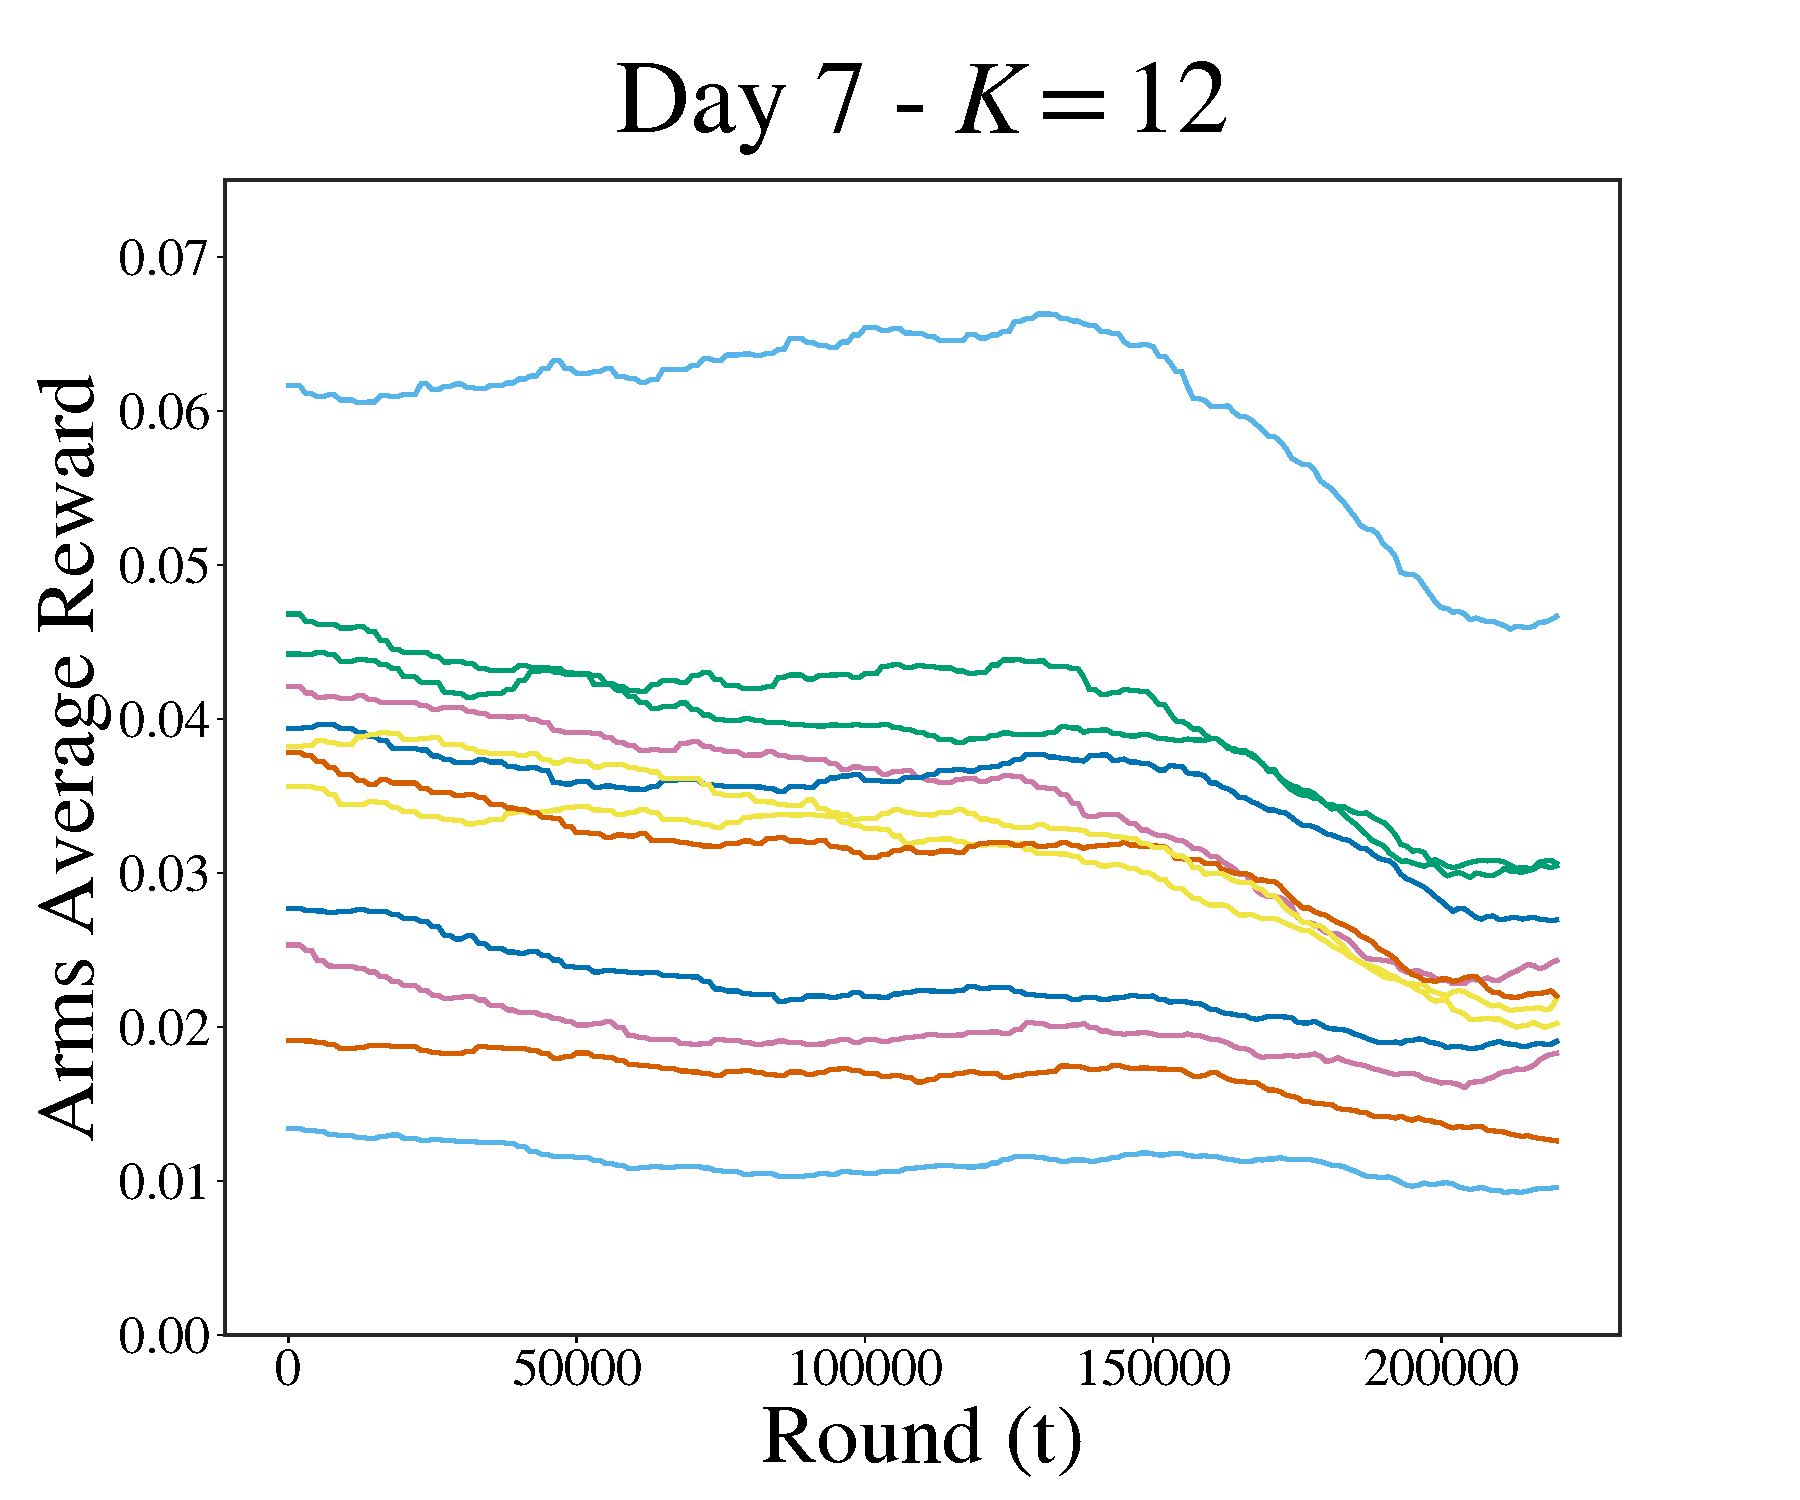
\includegraphics[clip, width= 0.495\textwidth]{4Restless/fig/reward_plot_day7.pdf}
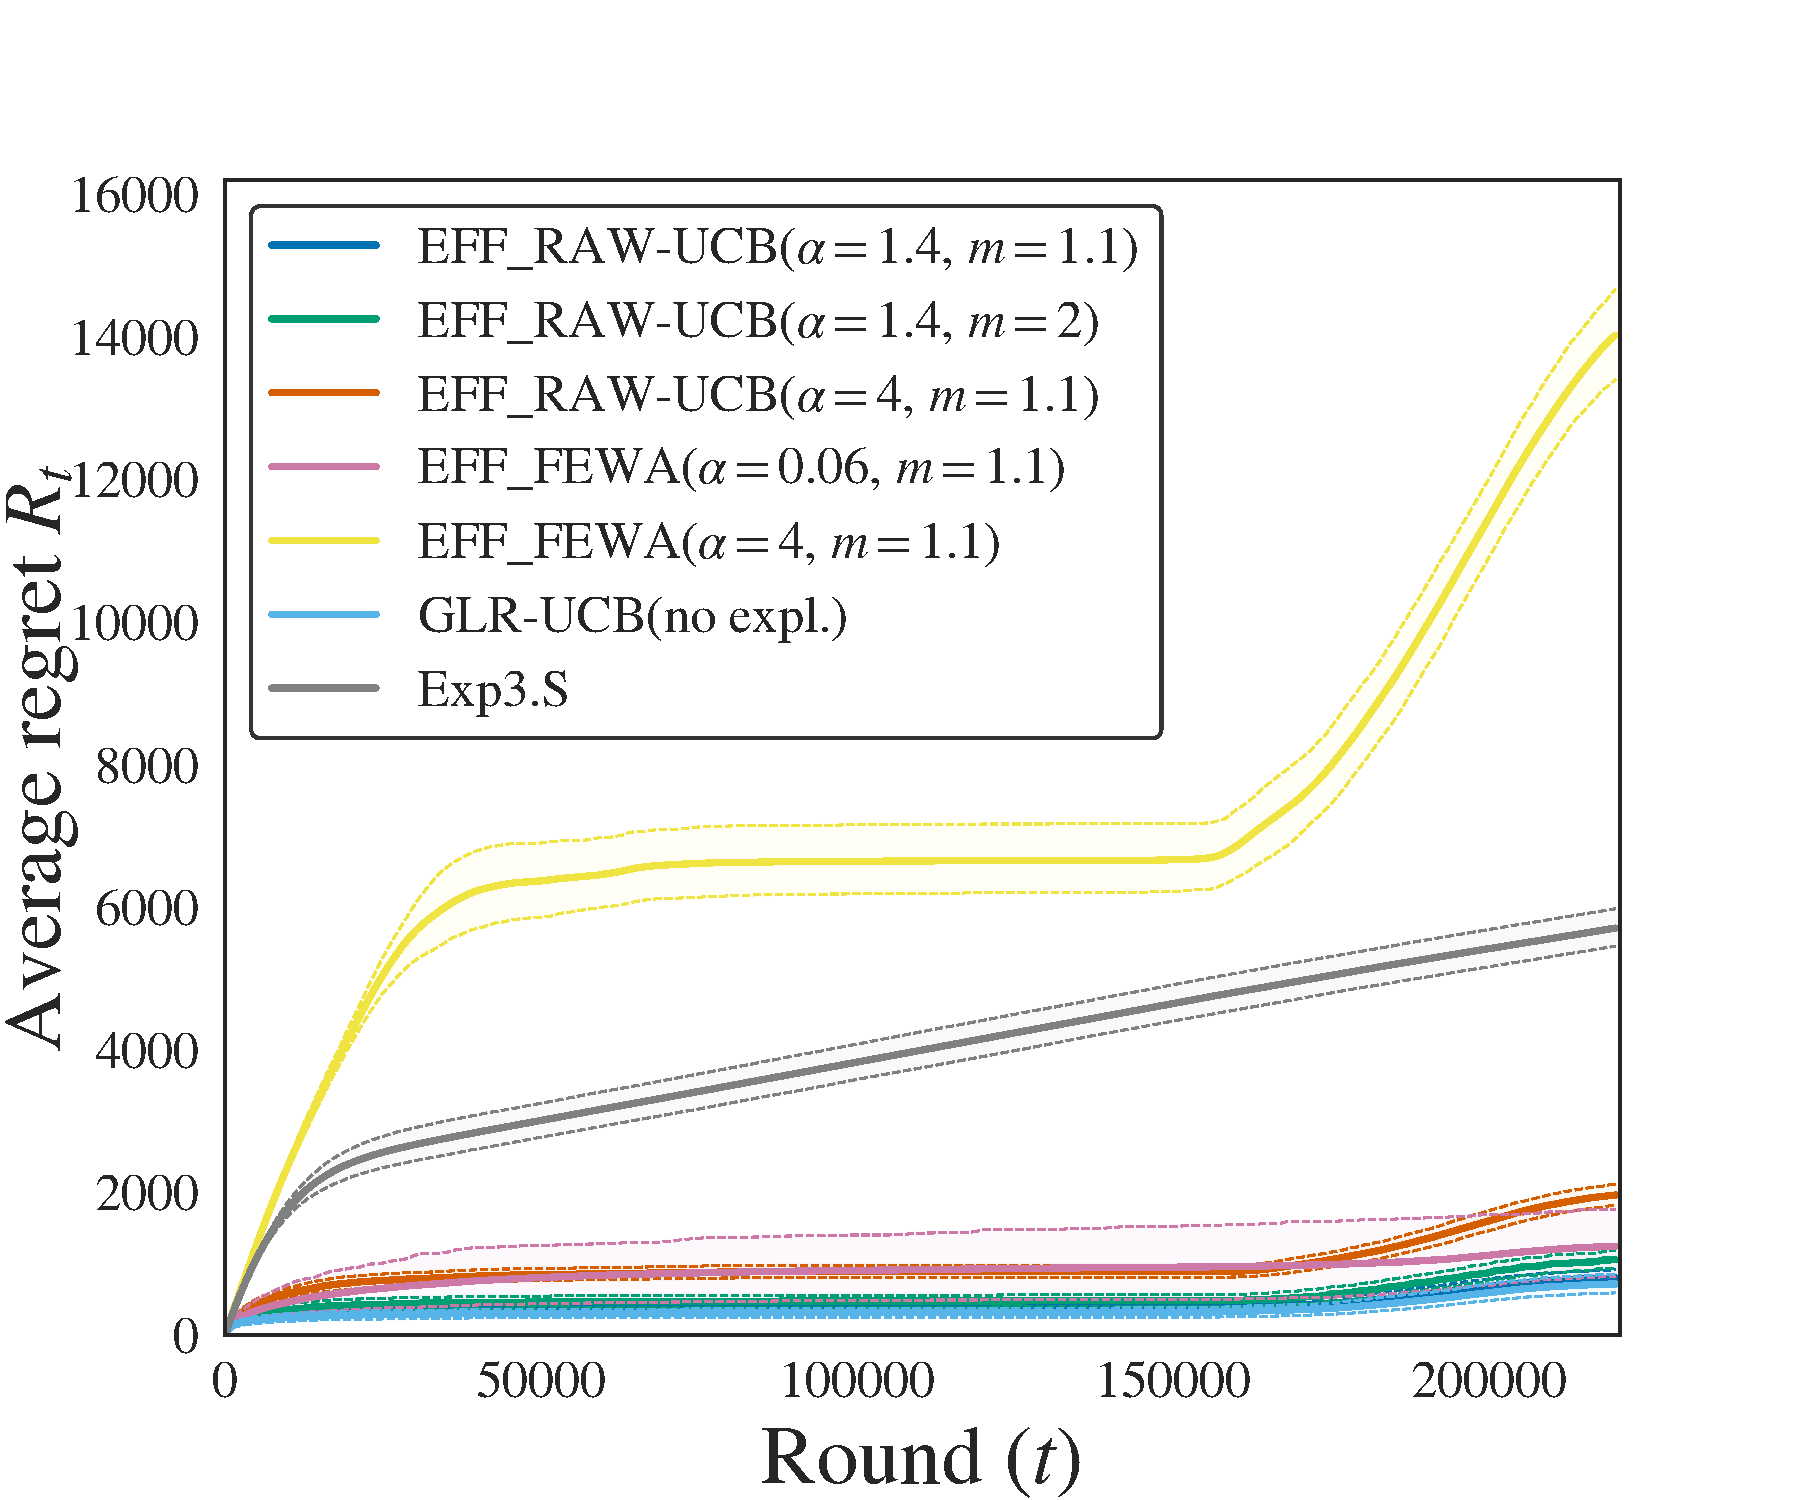
\includegraphics[clip, width= 0.495\textwidth]{4Restless/fig/DAY7.pdf}
\end{figure*}
\begin{figure*}[p!]
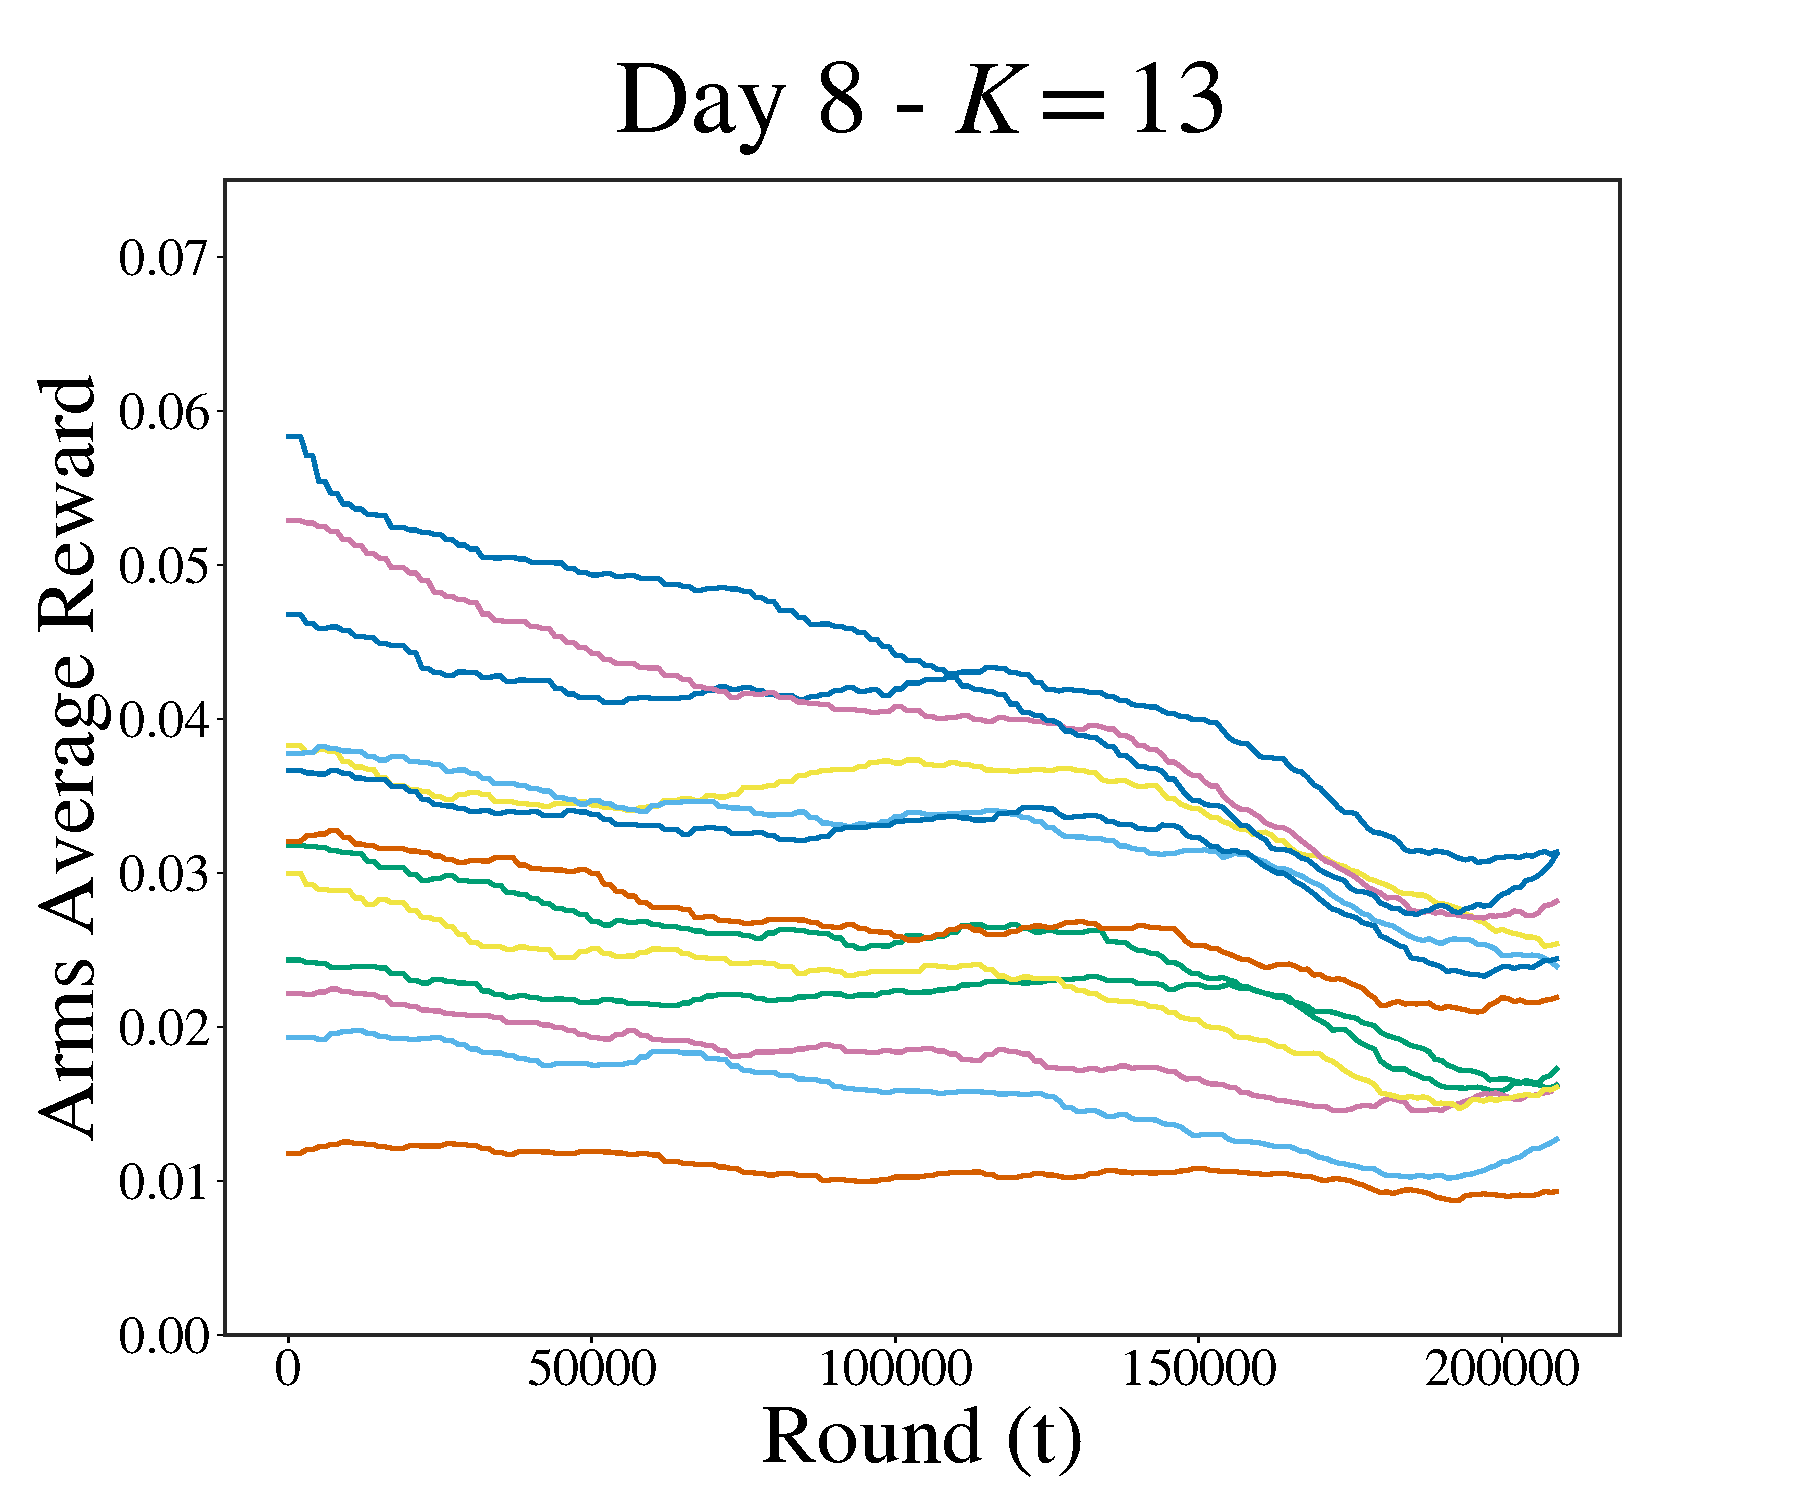
\includegraphics[clip, width= 0.495\textwidth]{4Restless/fig/reward_plot_day8.pdf}
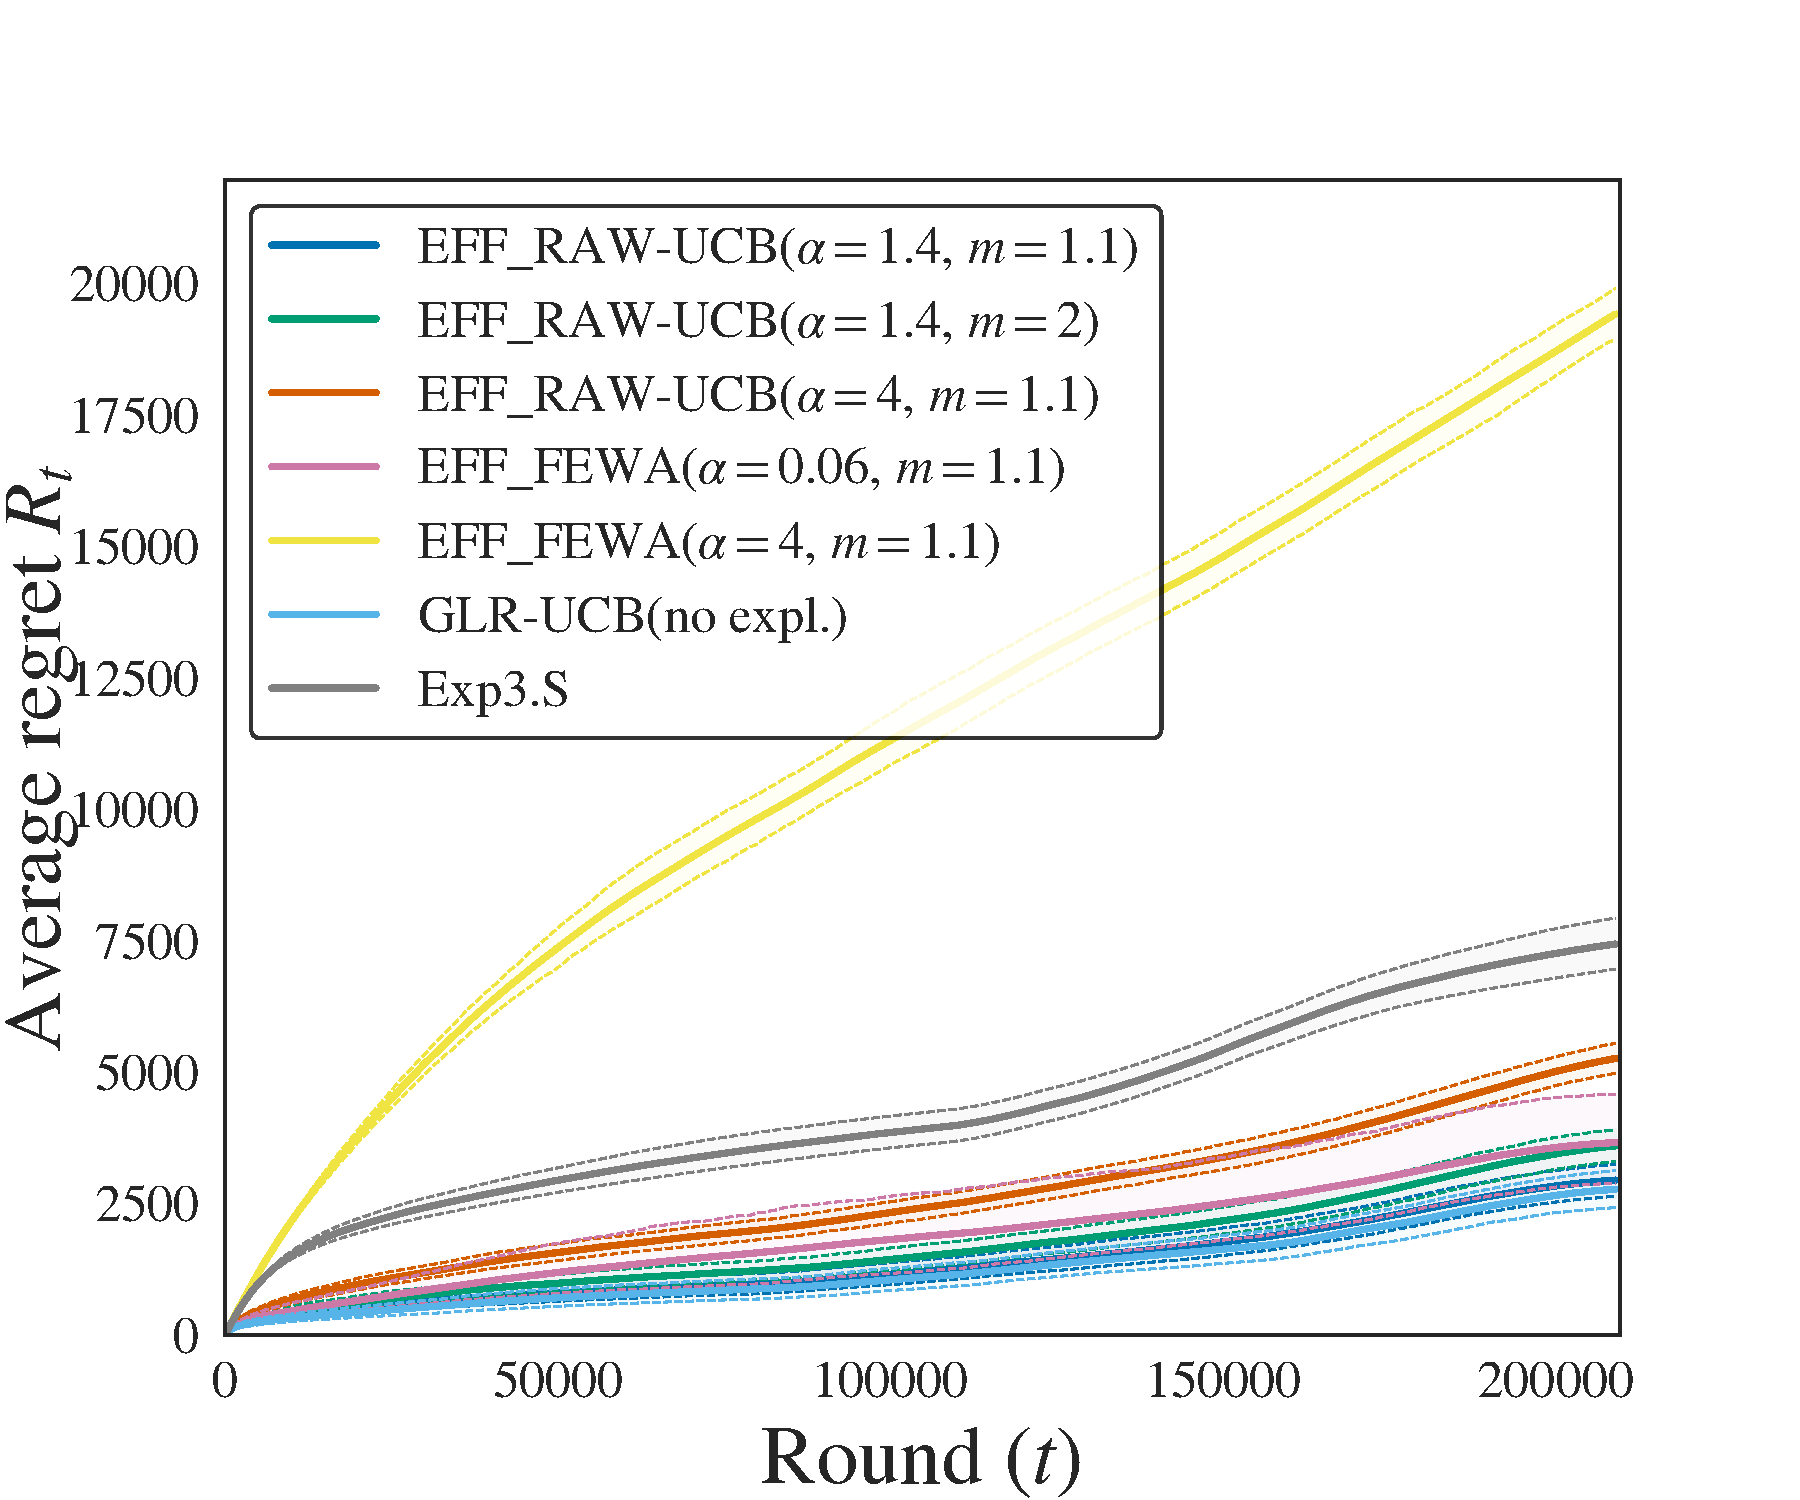
\includegraphics[clip, width= 0.495\textwidth]{4Restless/fig/DAY8.pdf}
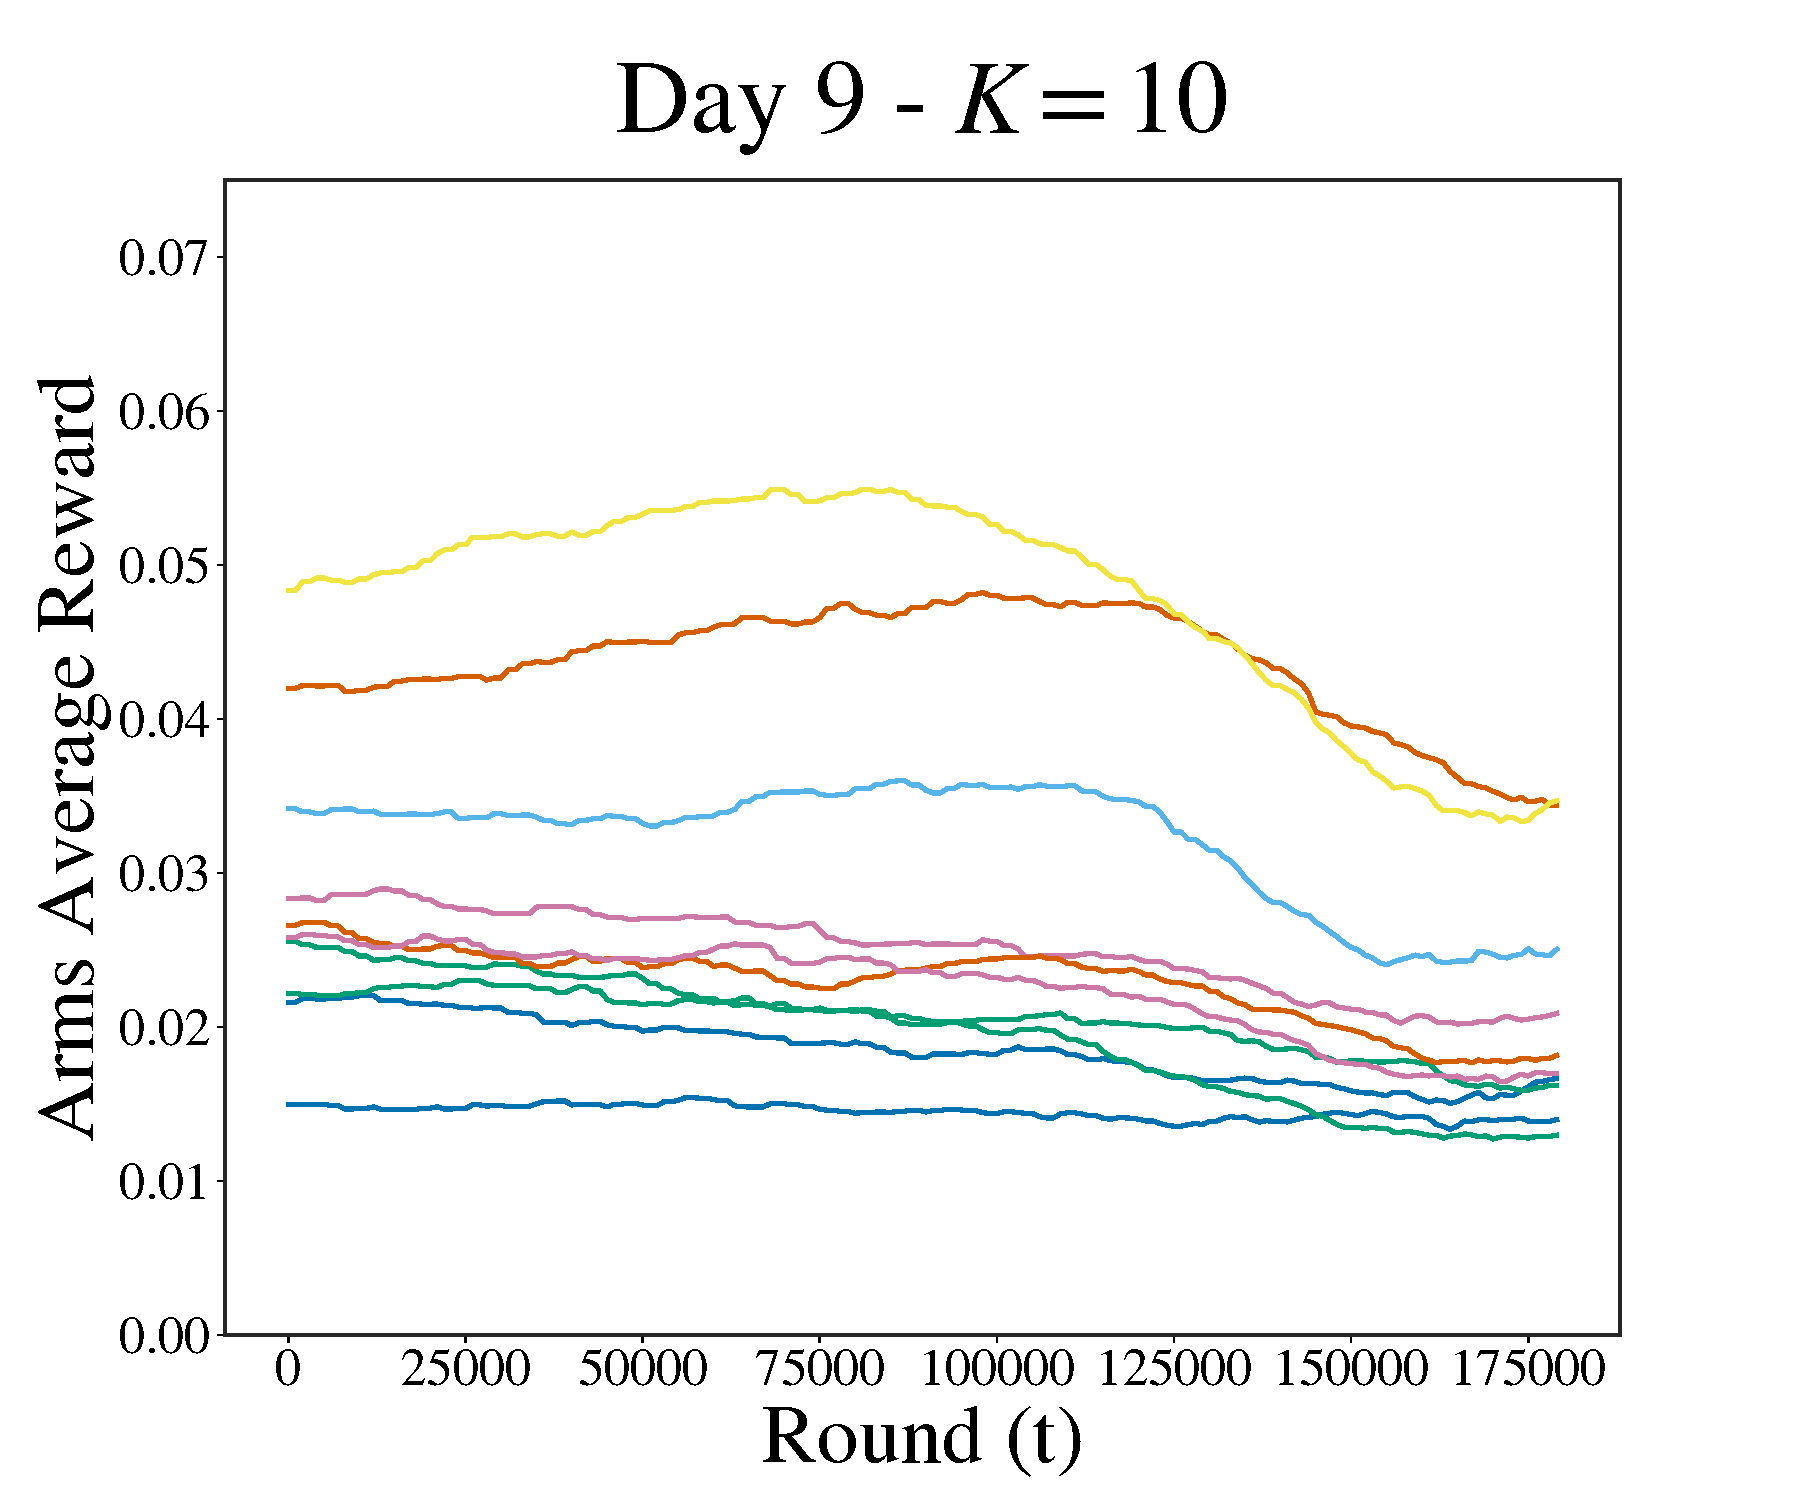
\includegraphics[clip, width= 0.495\textwidth]{4Restless/fig/reward_plot_day9.pdf}
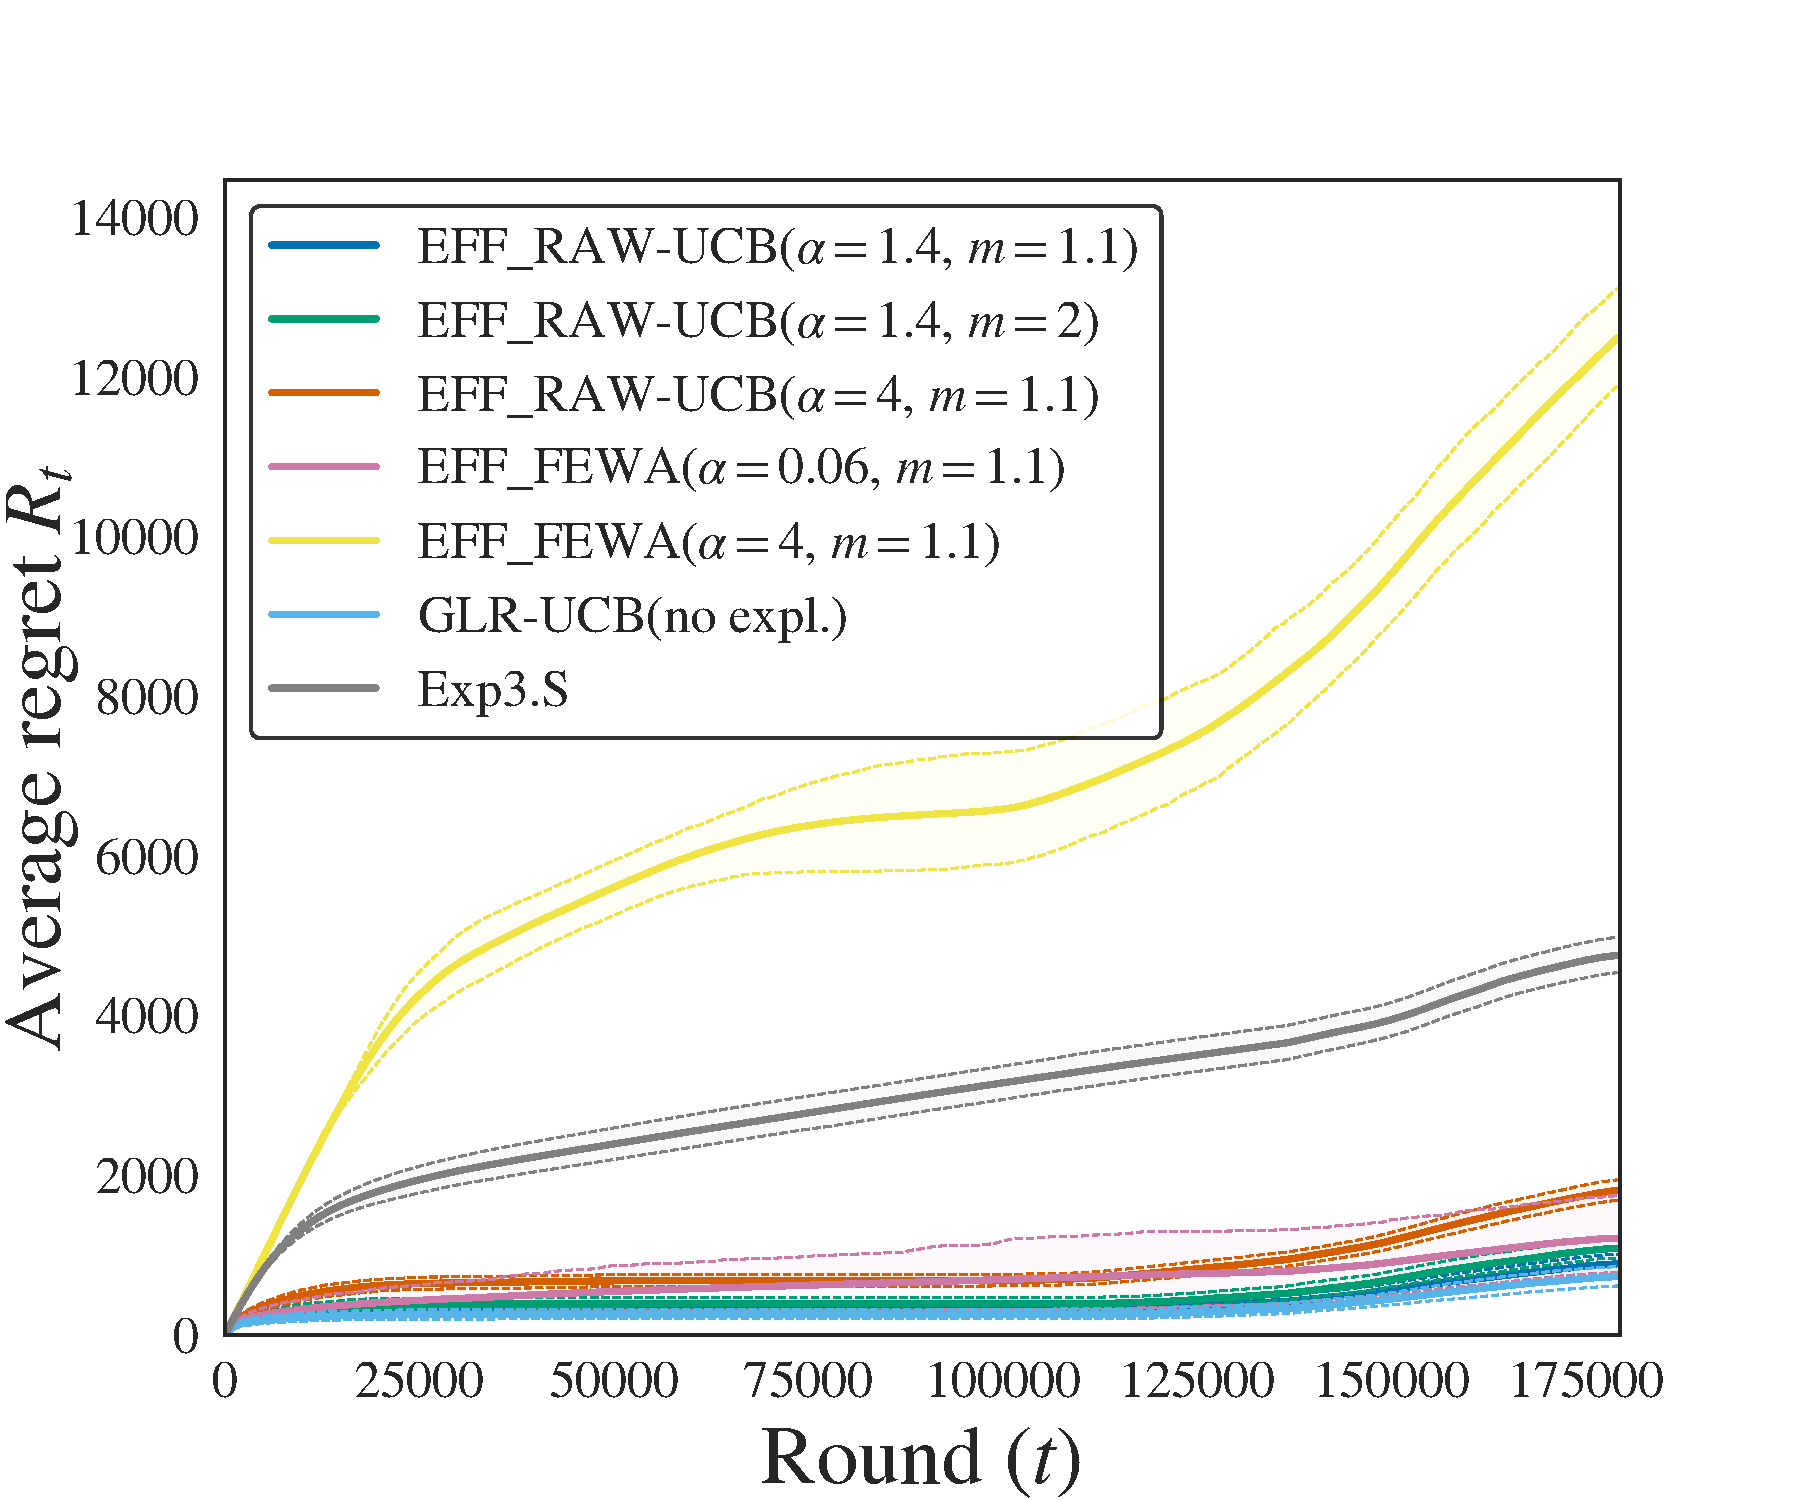
\includegraphics[clip, width= 0.495\textwidth]{4Restless/fig/DAY9.pdf}
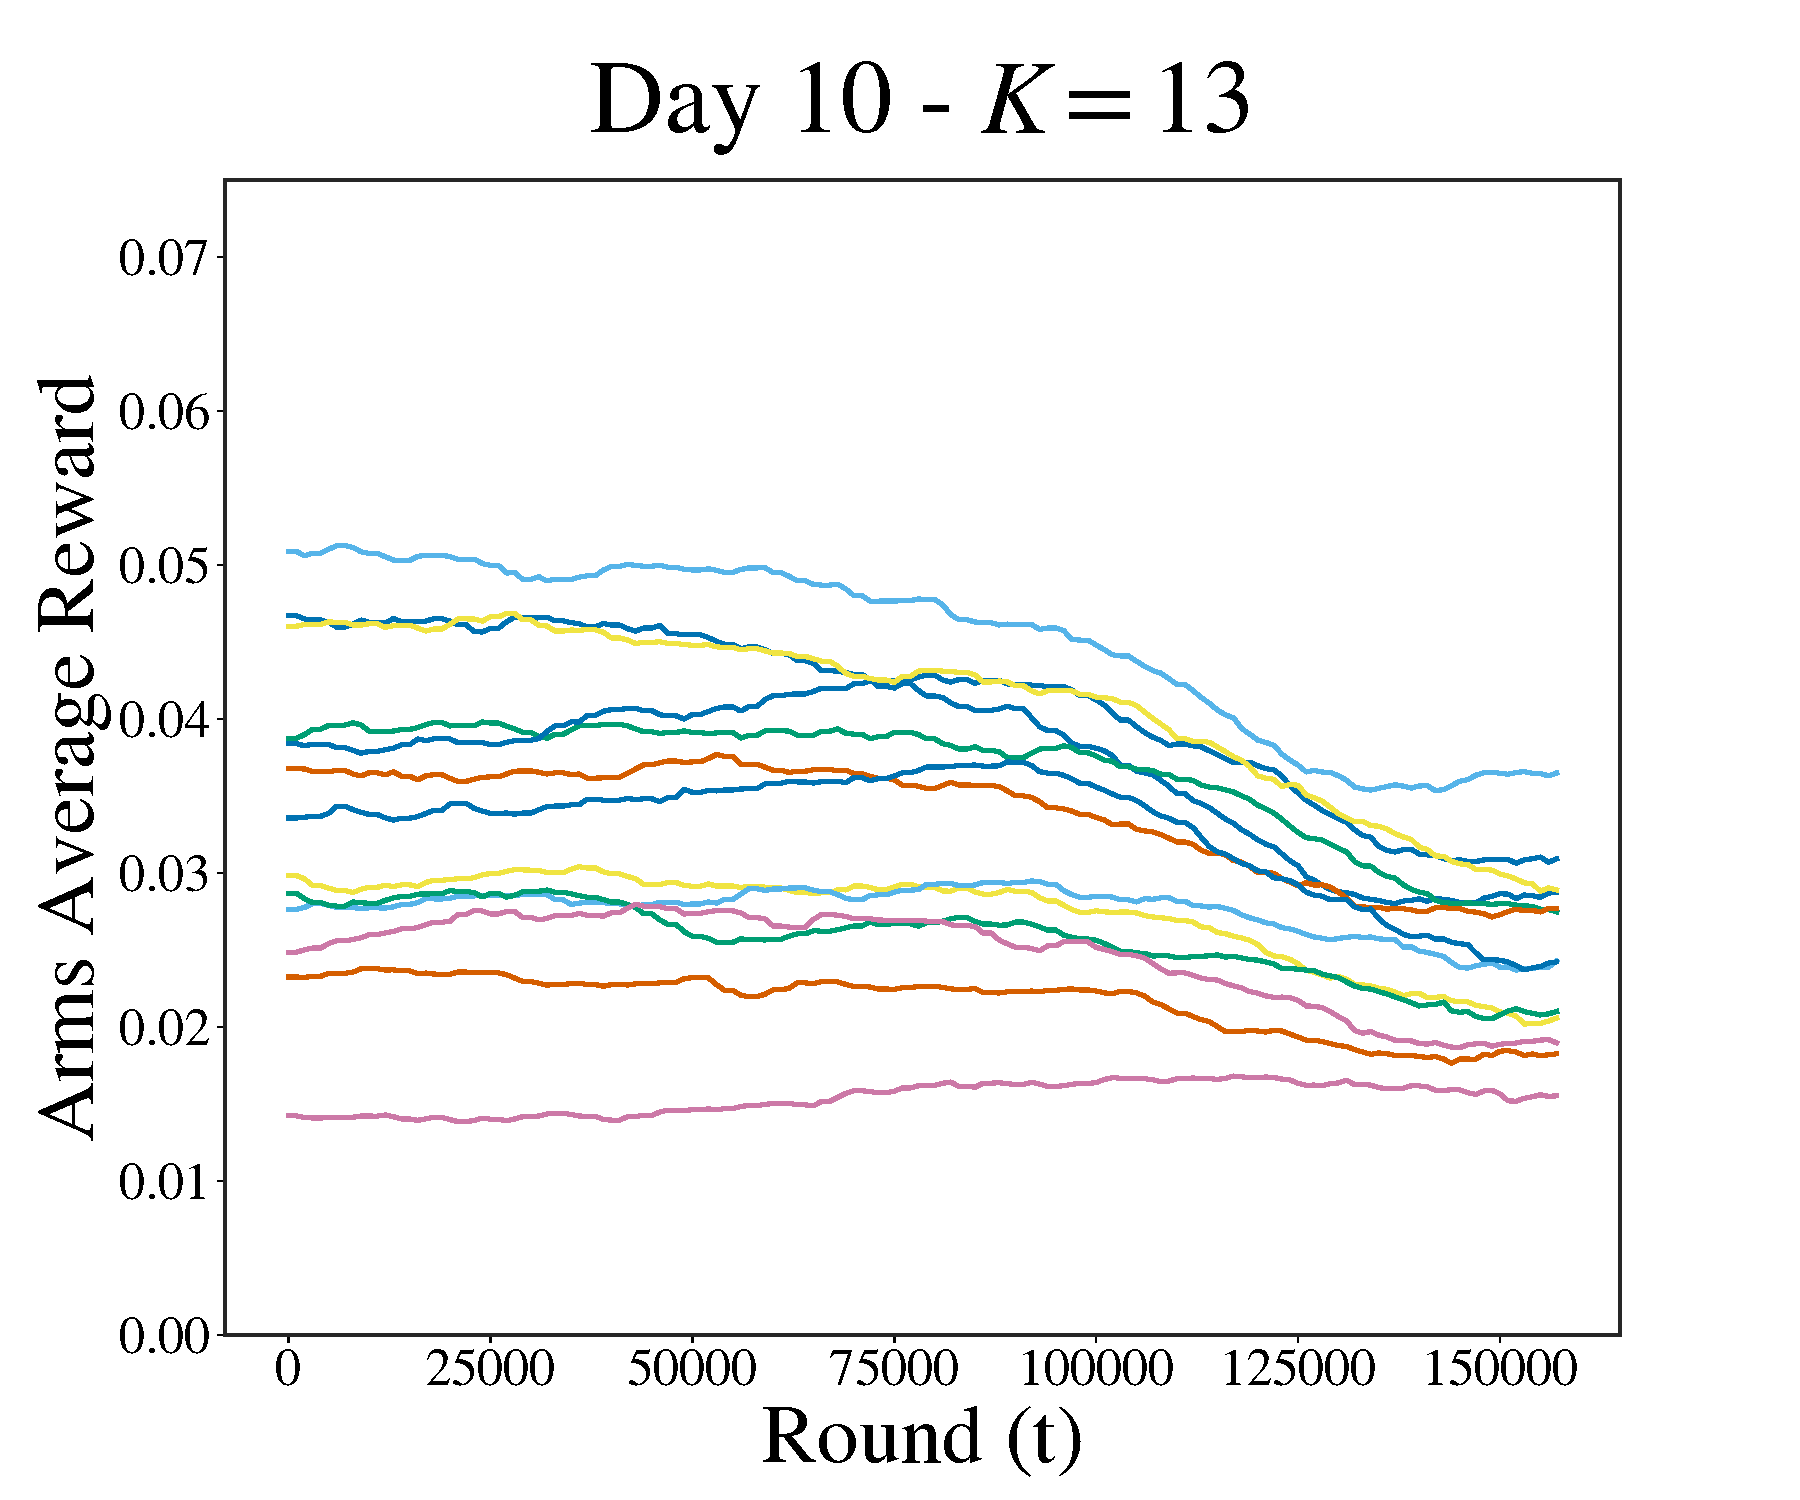
\includegraphics[clip, width= 0.495\textwidth]{4Restless/fig/reward_plot_day10.pdf}
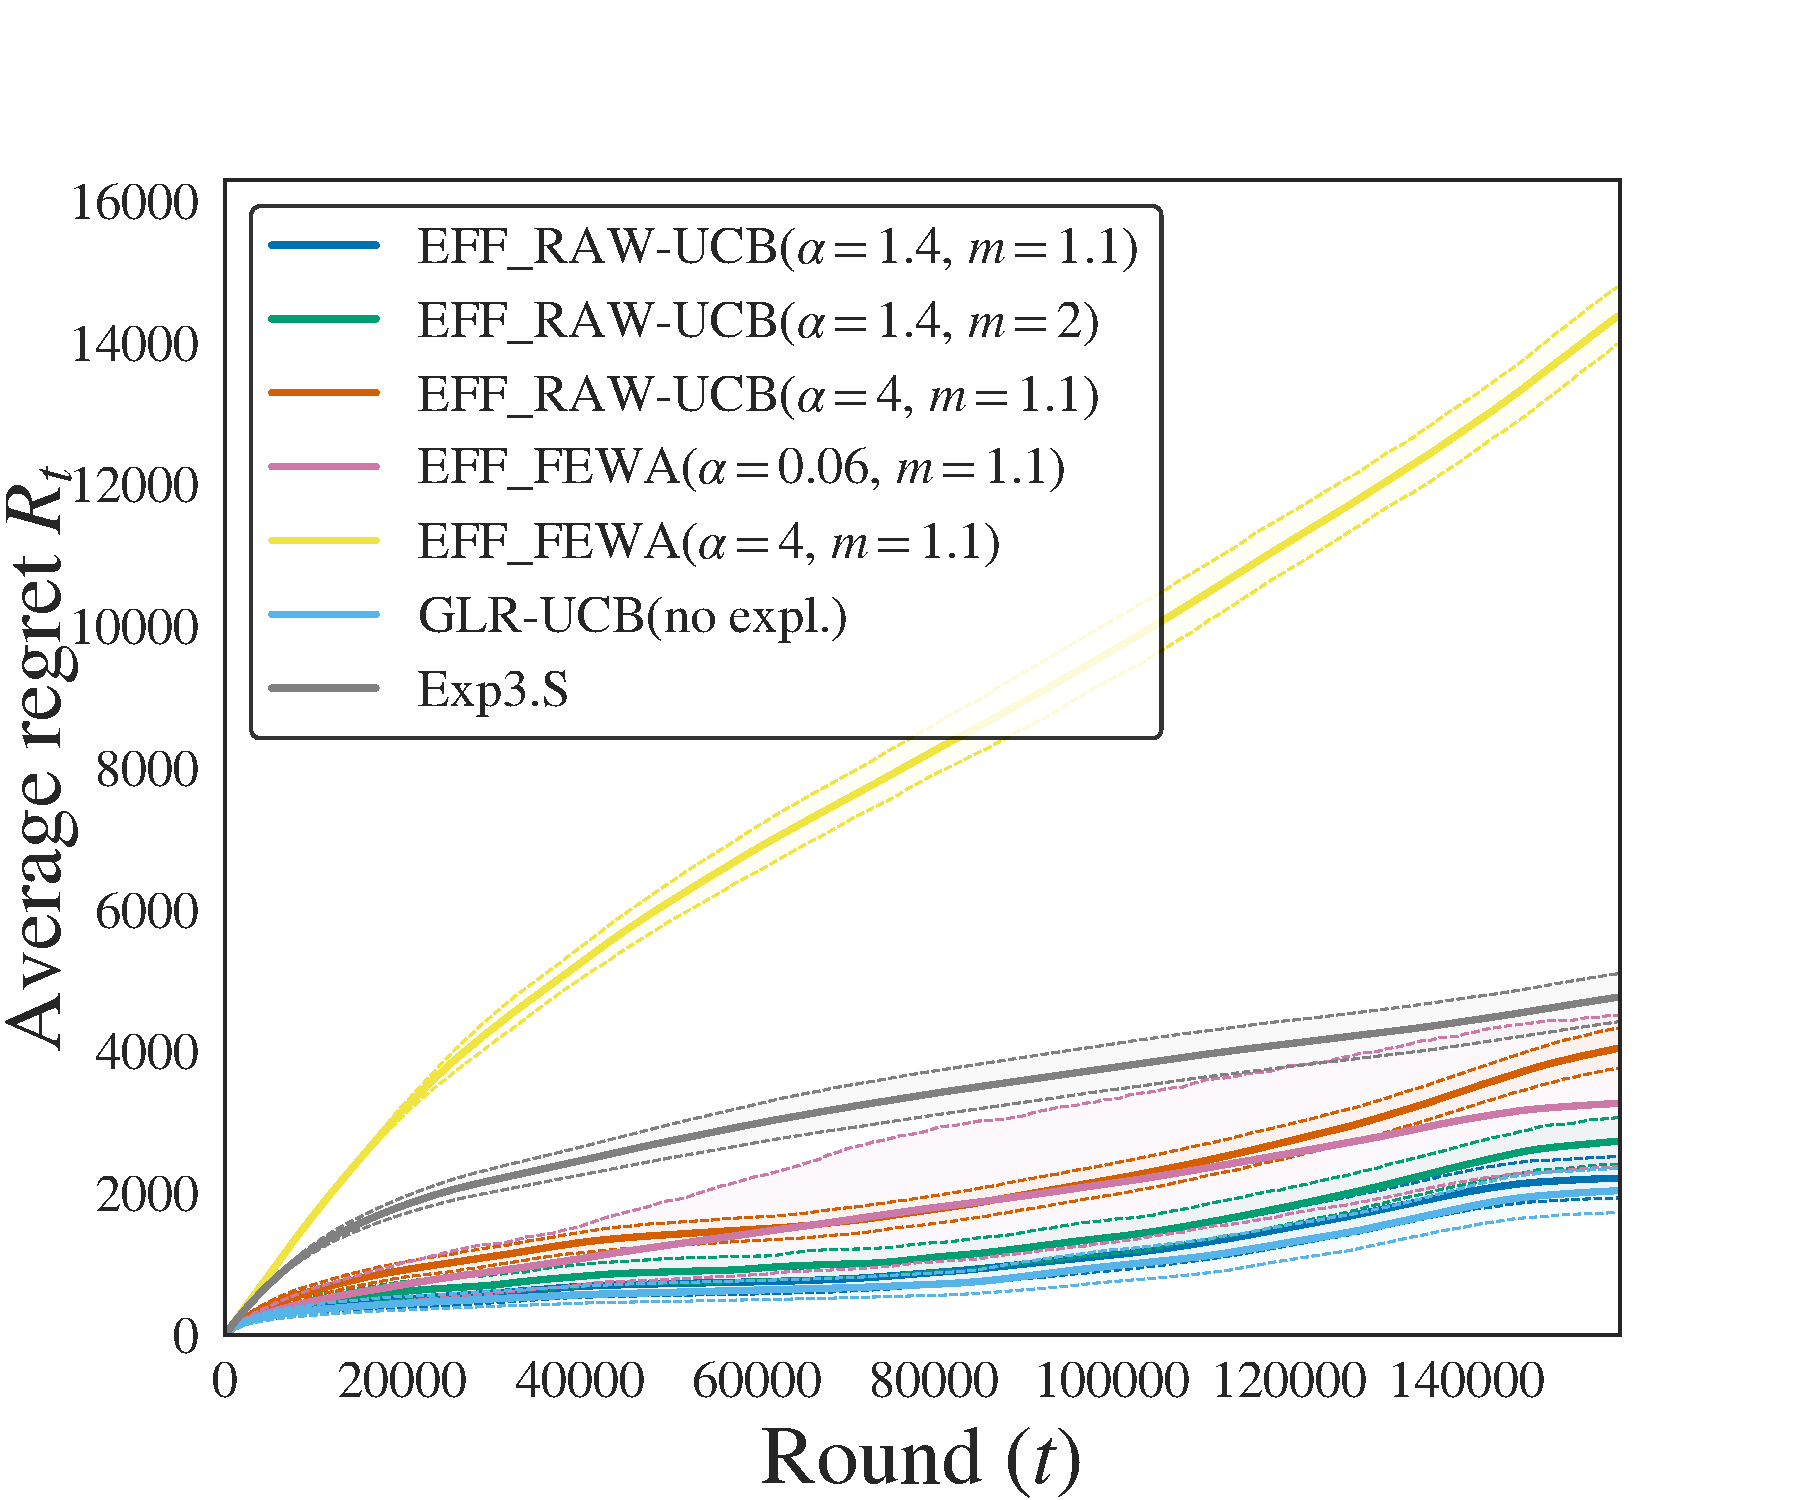
\includegraphics[clip, width= 0.495\textwidth]{4Restless/fig/DAY10.pdf}
\end{figure*}
\begin{table*}[ht!]
\begin{center}
\begin{tabular}{|@{\hskip3pt}c@{\hskip3pt}|@{\hskip5pt}c@{\hskip5pt}|@{\hskip5pt}c@{\hskip5pt}|@{\hskip5pt}c@{\hskip5pt}|@{\hskip5pt}c@{\hskip5pt}|@{\hskip5pt}c@{\hskip5pt}|@{\hskip5pt}c@{\hskip5pt}|@{\hskip5pt}c@{\hskip5pt}|@{\hskip5pt}c@{\hskip5pt}|@{\hskip5pt}c@{\hskip5pt}|}
\hline
\textbf{Day} & \textbf{2} & \textbf{3} & \textbf{4} & \textbf{5} & \textbf{6} & \textbf{7} & \textbf{8} & \textbf{9}              & \textbf{10}               \\ \hline
\!\EFFRAW\! \footnotesize{$\!(\alpha\!=\!1.4, m\!=\!1.1)\!$} \!& 67         & 66         & 90         & 86         & 91         & 74         & 88         & 64 & 48 \\  
\!\EFFRAW\!  {\footnotesize$(\alpha\!=\!1.4, m\!=\!2)$} \!  & 35         & 33         & 43         & 47         & 46         & 41         & 44         & 34   & 45 \\  
\!\EFFRAW \!{\footnotesize $(\alpha\!=\!4, m\!=\!1.1)$}\!   & 65         & 65         & 90         & 88         & 91         & 74         & 89         & 63 & 48  \\ \hline
\EFFFEWA \footnotesize{$(\alpha\!=\!0.06)$}           & 143        & 175        & 223        & 159        & 183        & 115        & 193        & 116        &       165       \\ 
\EFFFEWA \footnotesize{$(\alpha\!=\!4)$}              & 337        & 308        & 391        & 473        & 487        & 380        & 428        & 341     &  388               \\ \hline 
\EXPS   & 56         & 53         & 67         & 77         & 75         & 69         & 71         & 55      &   78 \\ \hline
\GLRUCB  & 560        & 613        & 683        & 2421       & 707        & 1529       & 957        & 971  & 4017\\ \hline
\end{tabular}
  \caption{Average computational time in seconds for each algorithm in each experiment.}
  \label{tab:restless-time}
\end{center}
\end{table*}

\paragraph{{\RAWUCB} vs {\FEWA}.} The two algorithms compute the same statistics and share most of their analysis. Yet, {\RAWUCB} consistently outperforms {\FEWA} as it was the case on the rested benchmark. The difference between the two is even more significant in the restless case. Its theoretical tuning $\alpha = 4$ gets reasonable results, while theoretical {\FEWA} is impractical. Finally, its empirical tuning $\alpha_{\mathrm{R}} =1.4$ is similar to the asymptotic optimal tuning of {\UCB} and shows good performance on both rested and restless problems. By contrast, {\FEWA} with $\alpha_{\mathrm{F}} = 0.06$ shows worse performance with larger deviation on the restless benchmark. 

\paragraph{{\RAWUCB} vs {\EXPS}.} {\EXPS} has good performances on the restless benchmark, on which it has theoretical guarantees. Yet, it is consistently outperformed by {\RAWUCB} when we tune the confidence bounds. It is particularly true in easy instances, e.g. on day 7. Indeed, in these cases, we expect a logarithmic regret rate for {\RAWUCB}.

\paragraph{{\RAWUCB} vs {\GLRUCB} (no active exploration).}  On the restless benchmark, {\GLRUCB} shows similar results than {\RAWUCB}. Yet, we highlight that 1) {\GLRUCB} needs the knowledge of the horizon to tune its change-detector; 2) we use an efficient version of {\RAWUCB} which runs $\sim 10$ times faster than {\GLRUCB}. In fact, the two algorithms are similar: they are UCB index policies, they recover logarithmic rate on easy restless rotting bandits problems and hence they would both suffer near-linear worst-case regret rate in the general restless setting (when active exploration is turned off for {\GLRUCB}). The main difference is that {\RAWUCB} scans its history to select its rotting UCB's window, while {\GLRUCB} scans its history to detect significant changes and restart. 


%!TEX root = ../main.tex
\section{Restless and rested rotting bandits}
\label{sec:general_decreasing_MAB_framework}
\subsection{The general case}
\begin{assumption}\label{assum:general}
For each arm $i$, any number of pulls $n$, and time $t$, the functions $\mu_i(t,\cdot)$ and $\mu_i(\cdot,n)$ are non-increasing.
\end{assumption}

In Section~\ref{sec:restless-theory}, we highlight that the main guarantee of our algorithms - Lemma~\ref{lem:core-full} -  holds in the general case of Assumption~\ref{assum:general}. Is it enough to show that our algorithms are near-optimal in this extended setup?

Like in Chapter~\ref{ch:rested} and~\ref{ch:restless}, we define the regret with respect to the best oracle.
\begin{equation*}
R_T(\pi, \mu) \triangleq \argmax_{\pi^\star_T \in \PiO}  J_T(\pi^\star_T, \mu) - J_T(\pi).
\end{equation*}

Like in the linear rested rotting bandits (Section~\ref{sec:linear-rotting}), we can show that not only the greedy oracle suffers linear regret but no learning policy can get a sublinear regret rate in the worst-case. 

\begin{proposition}
\label{prop:general-rotting-unlearnable}
In the no noise setting ($\sigma = 0$), there exists a rotting 2-arms bandits problem (satisfying Assumption~\ref{assum:general}) with reward value in $\left[0,1\right]$, with one rested arm and one restless arm, and with at most one change-point before $T$ each, such that the greedy oracle strategy $\pi_O$ suffers a regret 
\[R_T\pa{\pi_O} \geq \floor{\frac{T}{4}}.\]
Moreover, for any learning strategy  $\pi_S$, there exists a rotting 2-arms bandits problem (satisfying Assumption~\ref{assum:general}) with reward value in $\left[0,1\right]$, with one rested arm and one restless arm, and with at most one change-point before $T$ each, such that 
\[R_T\pa{\pi_S} \geq \floor{\frac{T}{8}}.\]
\end{proposition}

Notice that the two reward functions of the constructed difficult problems are simple: either rested or restless, bounded, and with at most one break-point. If we consider a 2-arm setup with one rested arm and one restless arm, a good strategy may be to select the restless arm even when its current value is the worst. Indeed, this value is only available now, while the good value of the rested arm will still be available in the future. Whether the restless rewards are interesting to the learner depends on the future behavior of the (currently best) rested arm. On the first hand, if it decays below the current value of the restless arm before $T$ pulls, then the learner should profit from the restless reward available right now. On the other hand, if the rested arm stays optimal until the end of the game then the learner should ignore the restless arm and follows the greedy oracle strategy. However, the learner does not know in advance if (and how much) an arm will decay and any anticipation she makes will turn to be bad in the worst case. We formalize these ideas in the proof at the end of the section.

\subsection{Rested rotting bandits with a restless envelope}
\begin{assumption}
\label{assum:envelop}
We consider the following reward functions, 
\[
\mu_i(t,n) = P(t) f_i(n) + S(t),
\]
where $P: \NN^* \rightarrow \R_+$, $\left\{f_i : \NN \rightarrow \R\right\}_{i \in \arms}$ and $S: \NN^* \rightarrow \R$ are non-increasing functions. 
\end{assumption}

Notice that all the arms have the same product $P$ and sum $S$ functions, the only difference is the rested evolution $f_i$. That is why we call this setup the rested rotting bandits with a restless envelope.

With this assumption, we can show that the greedy oracle is optimal.
\begin{proposition}
\label{prop:envelop}
For any reward functions $\left\{\mu_i\right\}_{i \in \arms}$ verifying Assumption~\ref{assum:envelop} and any horizon $T$, $\GO \in \argmax_{\pi \in \PiO} J_T(\pi)$.
\end{proposition}

We leave as an open problem to analyze the aforementioned algorithms in this setup. A first step would be to characterize the performance of the greedy bandit policy in the absence of noise (as we did for the rested problem, see Subsection~\ref{ss:rested-noiseless-online}). We may not recover the $\cO\pa{K}$ bound as in the rested setup. Indeed, the adversary can use the variation of $P$ and $S$ to trick the greedy bandit policy several times for each arm. Moreover, the order of the pull do matter in this problem: the cumulative reward is not a function of $\left\{\NiT\right\}_{i \in \arms}$ anymore.

\subsection{Proofs}
\label{ss:rested-restless-proofs}
\begin{proof}[Proof of Proposition~\ref{prop:general-rotting-unlearnable}]
Let $\mu^{0}$ and $\mu^{1}$, two decreasing 2-arms bandits problems such that:
\begin{align*}
 &\mu^{0}_1(t,n) = \mu_1(n) = 1 \text{ if } n<\frac{T}{2} \text{ else } 0\,,\\
 &\mu^{1}_1(t,n) = 1\,, \\
 &\mu^{0}_2(t,n) = \mu^{1}_2(t,n) = \mu_2(t) = 1/2 \text{ if } t<\frac{T}{2} \text{ else } 0.
\end{align*}
Problem $\mu^{1}$ only evolves according to time. Hence, the oracle greedy policy $\pi_O$ is optimal for this problem and collects
\begin{equation}
\label{eq:regret1-piO}
J_T\pa{\pi_O, \mu^1} = T.
\end{equation}
On $\mu^{0}$, $\pi_O$ selects arm $1$ during $\floor{\frac{T}{2}}$ rounds and then both arms yield $0$ reward. Thus, $\pi_O$ collects 
\[J_T\pa{\pi_O, \mu^0} = \floor{\frac{T}{2}}.\]
However, let $\pi_0$ the policy which selects arm 2 for $\floor{\frac{T}{2}}$ rounds and arm 1 afterwards. Thus, $\pi_0$ collects
\begin{equation}
\label{eq:regret0-pi0}
  J_T\pa{\pi_0, \mu^0} = \pa{3/2} \floor{\frac{T}{2}}.  
\end{equation}
Hence, we conclude the first part of our proposition, 
\[R_T\pa{\pi_O, \mu^0} = J_T\pa{\pi^\star_T, \mu^0} - J_T\pa{\pi_O, \mu^0} \geq J_T\pa{\pi_0, \mu^0} - J_T\pa{\pi_O, \mu^0} \geq  \floor{\frac{T}{4}}.\]
Now, we consider any learning policy $\pi_S$ and we call $\EEempty_j\big[N_{i,t}(\pi_S)\big]$ the (expected, if the policy is random) number of pulls of arm $i$ at any round $t$ by $\pi_S$ on problem $j$. Note that the leaner will receive the same rewards for both problems until at least $\floor{\frac{T}{2}}$. Therefore, we have that 

\[ \forall t \leq \floor{\frac{T}{2}}, \pi\big(\mathcal{H}_t\pa{\mu^0}\big) = \pi\big(\mathcal{H}_t\pa{\mu^1}\big) \implies \EEempty_0\Big[N_{2,\floor{\frac{T}{2}}}(\pi_S)\Big] = \EEempty_1\Big[N_{2,\floor{\frac{T}{2}}}(\pi_S)\Big] \triangleq n_2.\]

On problem $\mu^{1}$, $\pi_S$ collects a reward of at most,
\begin{equation}
\label{eq:regret1-piS}
    J_T\pa{\pi_S, \mu^1} = \EEempty_1[N_{1,T}(\pi_S)] + \frac{n_2}{2} = T - \EEempty_1[N_{2,T}(\pi_S)] + \frac{n_2}{2} \leq T - \frac{n_2}{2}\CommaBin
\end{equation}
because $n_2 = \EEempty_1\Big[N_{2,\floor{\frac{T}{2}}}(\pi_S)\Big] \leq \EEempty_1[N_{2,T}(\pi_S)]$. Using Equations~\ref{eq:regret1-piO} and~\ref{eq:regret1-piS}, we can lower bound the regret of $\pi_S$, 
\[ R_T\pa{\pi_S, \mu^1} = J_T\pa{\pi_O, \mu^1} - J_T\pa{\pi_S, \mu^1} \geq  \frac{n_2}{2}\cdot \]


On problem $\mu^{0}$, $\pi_S$ collects a reward of at most,
\begin{equation}
\label{eq:regret0-piS}
    J_T\pa{\pi_S, \mu^0} = \min\pa{\EEempty_1[N_{1,T}(\pi_S)],\floor{\frac{T}{2}}} + \frac{n_2}{2} \leq \floor{\frac{T}{2}} + \frac{n_2}{2}\cdot
\end{equation}
Using Equations~\ref{eq:regret0-pi0} and~\ref{eq:regret0-piS}, we can lower bound the regret of $\pi_S$, 
\[ R_T\pa{\pi_S, \mu^0} = J_T\pa{\pi_O, \mu^0} - J_T\pa{\pi_S, \mu^0} \geq  \frac{\floor{T/2} - n_2}{2}\cdot \]

Hence, the worst case regret on the two setups is bounded by 
\[R_T(\pi_S) \geq \max\pa{\frac{n_2}{2}, \frac{\floor{\frac{T}{2}} - n_2}{2}} \geq \floor{\frac{T}{8}}\!\cdot \]
\end{proof}

\begin{proof}[Proof of Proposition~\ref{prop:envelop}]
At any round $t$, we have,
\[
\GO(t) \in \argmax_{i \in \arms} \pa{P(t)f_i(\Nit) + S(t)} = \argmax_{i \in \arms} f_i \pa{\Nit}.
\] 
Therefore, at round $t$, collects the $t$ largest values of $\ev{f_i(n)}_{i\in \arms, n\leq T}$, \textit{i.e.} 
\[
\forall i \in \arms, \ \forall n_i \geq \Nit, \ \mu_{\GO(t)}\pa{N_{\GO(t),\,t}} \geq\mu_{i}\pa{\Nit}  \geq \mu_i(n_i).
\]

The first inequality is due to the selection rule of the policy; the second is due to the decreasing reward functions. 

A direct consequence is that, at the round $t$, $\GO$ selects the $t$-th largest value of $\left\{f_i(n)\right\}_{i \in \arms, n \leq T}$. Hence, at the round $T$, it has selected the $T$ largest value in the decreasing order. Since $P(t)$ is non-increasing and positive, an other policy which selects smaller values of $\left\{f_i(n)\right\}_{i \in \arms, n \leq T}$, or the same values but in an other order, have a smaller or equal cumulative reward than $\GO$.
\end{proof}

\documentclass[12pt,fleqn]{book} % Default font size and left-justified equations

% !TEX root = main.tex


%%%%%%%%%%%%%%%%%%%%%%%%%%%%%%%%%%%%%%%%%
% The Legrand Orange Bookbookmarks=true,
% Structural Definitions File
% Version 2.0 (9/2/15)
%
% Original author:
% Mathias Legrand (legrand.mathias@gmail.com) with modifications by:
% Vel (vel@latextemplates.com)
% 
% This file has been downloaded from:
% http://www.LaTeXTemplates.com
%
% License:
% CC BY-NC-SA 3.0 (http://creativecommons.org/licenses/by-nc-sa/3.0/)
%
%%%%%%%%%%%%%%%%%%%%%%%%%%%%%%%%%%%%%%%%%

%----------------------------------------------------------------------------------------
%	VARIOUS REQUIRED PACKAGES AND CONFIGURATIONS
%----------------------------------------------------------------------------------------
\usepackage[top=3cm,bottom=3cm,left=3cm,right=3cm,headsep=10pt,a4paper]{geometry} % Page margins

\usepackage{graphicx} % Required for including pictures
\graphicspath{{fig/}} % Specifies the directory where pictures are stored

\usepackage{tikz} % Required for drawing custom shapes

%\usepackage[english]{babel} % English language/hyphenation

\usepackage{enumitem} % Customize lists
\setlist{nolistsep} % Reduce spacing between bullet points and numbered lists

\usepackage{booktabs} % Required for nicer horizontal rules in tables

\usepackage{xcolor} % Required for specifying colors by name
\definecolor{ocre}{RGB}{243,102,25} % Define the orange color used for highlighting throughout the book
\definecolor{myBlue}{RGB}{3,146,207} % Define the orange color used for highlighting throughout the book


%----------------------------------------------------------------------------------------
%	FONTS
%----------------------------------------------------------------------------------------

\usepackage{avant} % Use the Avantgarde font for headings
%\usepackage{times} % Use the Times font for headings
\usepackage{mathptmx} % Use the Adobe Times Roman as the default text font together with math symbols from the Sym­bol, Chancery and Com­puter Modern fonts

\usepackage{microtype} % Slightly tweak font spacing for aesthetics
\usepackage[utf8]{inputenc} % Required for including letters with accents
\usepackage[T1]{fontenc} % Use 8-bit encoding that has 256 glyphs

%----------------------------------------------------------------------------------------
%	BIBLIOGRAPHY AND INDEX
%----------------------------------------------------------------------------------------

\usepackage[style=authoryear-comp,uniquelist=false,citestyle=authoryear,sorting=ynt,sortcites=true,autopunct=true,babel=hyphen,hyperref,abbreviate=false,backref=true,backend=biber,maxcitenames=2,maxbibnames=20]{biblatex}
%\usepackage[style=authoryear-comp,citestyle=authoryear,sorting=nyt,sortcites=true,autopunct=true,babel=hyphen,hyperref,abbreviate=false,backref=true,backend=biber,maxcitenames=20]{biblatex}
\addbibresource{other_tex_files/PhD_Thesis_Julien_Seznec.bib} % BibTeX bibliography file
\defbibheading{bibempty}{}

\usepackage{calc} % For simpler calculation - used for spacing the index letter headings correctly
\usepackage{makeidx} % Required to make an index
\makeindex % Tells LaTeX to create the files required for indexing

%----------------------------------------------------------------------------------------
%	MAIN TABLE OF CONTENTS
%----------------------------------------------------------------------------------------

\usepackage{titletoc} % Required for manipulating the table of contents
%\usepackage{morewrites} % fix no room for new write error with tablecontent+listofalgorithms clash
\contentsmargin{0cm} % Removes the default margin

% Part text styling
\titlecontents{part}[0cm]
{\addvspace{20pt}\centering\large\bfseries}
{}
{}
{}

% Chapter text styling
\titlecontents{chapter}[1.25cm] % Indentation
{\addvspace{12pt}\large\sffamily\bfseries} % Spacing and font options for chapters
{\color{myBlue!60}\contentslabel[\Large\thecontentslabel]{1.25cm}\color{myBlue}} % Chapter number
{\color{myBlue}}  
{\color{myBlue!60}\normalsize\;\titlerule*[.5pc]{.}\;\thecontentspage} % Page number

% Section text styling
\titlecontents{section}[1.25cm] % Indentation
{\addvspace{3pt}\sffamily\bfseries} % Spacing and font options for sections
{\contentslabel[\thecontentslabel]{1.25cm}} % Section number
{}
{\hfill\color{black}\thecontentspage} % Page number
[]

% Subsection text styling
\titlecontents{subsection}[1.25cm] % Indentation
{\addvspace{1pt}\sffamily\small} % Spacing and font options for subsections
{\contentslabel[\thecontentslabel]{1.25cm}} % Subsection number
{}
{\ \titlerule*[.5pc]{.}\;\thecontentspage} % Page number
[]

% List of figures
\titlecontents{figure}[0em]
{\addvspace{-5pt}\sffamily}
{\thecontentslabel\hspace*{1em}}
{}
{\ \titlerule*[.5pc]{.}\;\thecontentspage}
[]

% List of tables
\titlecontents{table}[0em]
{\addvspace{-5pt}\sffamily}
{\thecontentslabel\hspace*{1em}}
{}
{\ \titlerule*[.5pc]{.}\;\thecontentspage}
[]

% List of algorithms
\titlecontents{algorithm}[0em]
{\addvspace{-5pt}\sffamily}
{\thecontentslabel\hspace*{1em}}
{}
{\ \titlerule*[.5pc]{.}\;\thecontentspage}
[]

%----------------------------------------------------------------------------------------
%	MINI TABLE OF CONTENTS IN PART HEADS
%----------------------------------------------------------------------------------------

% Chapter text styling
\titlecontents{lchapter}[0em] % Indenting
{\addvspace{15pt}\large\sffamily\bfseries} % Spacing and font options for chapters
{\color{myBlue}\contentslabel[\Large\thecontentslabel]{1.25cm}\color{myBlue}} % Chapter number
{}  
{\color{myBlue}\normalsize\sffamily\bfseries\;\titlerule*[.5pc]{.}\;\thecontentspage} % Page number

% Section text styling
\titlecontents{lsection}[0em] % Indenting
{\sffamily\small} % Spacing and font options for sections
{\contentslabel[\thecontentslabel]{1.25cm}} % Section number
{}
{}

% Subsection text styling
\titlecontents{lsubsection}[.5em] % Indentation
{\normalfont\footnotesize\sffamily} % Font settings
{}
{}
{}

%----------------------------------------------------------------------------------------
%	PAGE HEADERS
%----------------------------------------------------------------------------------------

\usepackage{fancyhdr} % Required for header and footer configuration

\pagestyle{fancy}
\renewcommand{\chaptermark}[1]{\markboth{\sffamily\normalsize\bfseries\chaptername\ \thechapter.\ #1}{}} % Chapter text font settings
\renewcommand{\sectionmark}[1]{\markright{\sffamily\normalsize\thesection\hspace{5pt}#1}{}} % Section text font settings
\fancyhf{} \fancyhead[LE,RO]{\sffamily\normalsize\thepage} % Font setting for the page number in the header
\fancyhead[LO]{\rightmark} % Print the nearest section name on the left side of odd pages
\fancyhead[RE]{\leftmark} % Print the current chapter name on the right side of even pages
\renewcommand{\headrulewidth}{0.5pt} % Width of the rule under the header
\addtolength{\headheight}{2.5pt} % Increase the spacing around the header slightly
\renewcommand{\footrulewidth}{0pt} % Removes the rule in the footer
\fancypagestyle{plain}{\fancyhead{}\renewcommand{\headrulewidth}{0pt}} % Style for when a plain pagestyle is specified

% Removes the header from odd empty pages at the end of chapters
\makeatletter
\renewcommand{\cleardoublepage}{
\clearpage\ifodd\c@page\else
\hbox{}
\vspace*{\fill}
\thispagestyle{empty}
\newpage
\fi}

%----------------------------------------------------------------------------------------
%	THEOREM STYLES
%----------------------------------------------------------------------------------------

\usepackage{amsmath,amsfonts,amssymb,amsthm} % For math equations, theorems, symbols, etc
\usepackage{environ}
\usepackage{thmtools}
\usepackage{thm-restate}
\AfterEndEnvironment{restatable}{\noindent\ignorespaces}
\newcommand{\intoo}[2]{\mathopen{]}#1\,;#2\mathclose{[}}
\newcommand{\ud}{\mathop{\mathrm{{}d}}\mathopen{}}
\newcommand{\intff}[2]{\mathopen{[}#1\,;#2\mathclose{]}}
\newtheorem{notation}{Notation}[chapter]

% Boxed/framed environments
\newtheoremstyle{ocrenumbox}% % Theorem style name
{10pt}% Space above
{0pt}% Space below
{\normalfont}% % Body font
{}% Indent amount
{\small\bf\sffamily\color{myBlue}}% % Theorem head font
{\;}% Punctuation after theorem head
{0.25em}% Space after theorem head
{\small\sffamily\color{myBlue}\thmname{#1}\nobreakspace\thmnumber{\@ifnotempty{#1}{}\@upn{#2}}% Theorem text (e.g. Theorem 2.1)
\thmnote{\nobreakspace\the\thm@notefont\sffamily\bfseries\color{black}---\nobreakspace#3.}} % Optional theorem note
\renewcommand{\qedsymbol}{$\blacksquare$}% Optional qed square

\newtheoremstyle{blacknumex}% Theorem style name
{10pt}% Space above
{0pt}% Space below
{\normalfont}% Body font
{} % Indent amount
{\small\bf\sffamily}% Theorem head font
{\;}% Punctuation after theorem head
{0.25em}% Space after theorem head
{\small\sffamily{\tiny\ensuremath{\blacksquare}}\nobreakspace\thmname{#1}\nobreakspace\thmnumber{\@ifnotempty{#1}{}\@upn{#2}}% Theorem text (e.g. Theorem 2.1)
\thmnote{\nobreakspace\the\thm@notefont\sffamily\bfseries---\nobreakspace#3.}}% Optional theorem note

\newtheoremstyle{blacknumbox} % Theorem style name
{0pt}% Space above
{0pt}% Space below
{\normalfont}% Body font
{}% Indent amount
{\small\bf\sffamily}% Theorem head font
{\;}% Punctuation after theorem head
{0.25em}% Space after theorem head
{\small\sffamily\thmname{#1}\nobreakspace\thmnumber{\@ifnotempty{#1}{}\@upn{#2}}% Theorem text (e.g. Theorem 2.1)
\thmnote{\nobreakspace\the\thm@notefont\sffamily\bfseries---\nobreakspace#3.}}% Optional theorem note

% Non-boxed/non-framed environments
\newtheoremstyle{ocrenum}% % Theorem style name
{5pt}% Space above
{5pt}% Space below
{\normalfont}% % Body font
{}% Indent amount
{\small\bf\sffamily\color{myBlue}}% % Theorem head font
{\;}% Punctuation after theorem head
{0.25em}% Space after theorem head
{\small\sffamily\color{myBlue}\thmname{#1}\nobreakspace\thmnumber{\@ifnotempty{#1}{}\@upn{#2}}% Theorem text (e.g. Theorem 2.1)
\thmnote{\nobreakspace\the\thm@notefont\sffamily\bfseries\color{black}---\nobreakspace#3.}} % Optional theorem note
\renewcommand{\qedsymbol}{$\blacksquare$}% Optional qed square
\makeatother

% Defines the theorem text style for each type of theorem to one of the three styles above
\newcounter{dummy} 
\numberwithin{dummy}{section}
\theoremstyle{ocrenumbox}
\newtheorem{theoremeT}[dummy]{Theorem}
\newtheorem{problem}{Problem}[chapter]
\newtheorem{exerciseT}{Exercise}[chapter]
\theoremstyle{blacknumex}
\newtheorem{exampleT}{Example}[chapter]
\theoremstyle{blacknumbox}
\newtheorem{vocabulary}{Vocabulary}[chapter]
\newtheorem{definitionT}{Definition}[section]
\newtheorem{corollaryT}[dummy]{Corollary}
\theoremstyle{ocrenum}
\newtheorem{proposition}[dummy]{Proposition}
\newtheorem{lemma}[dummy]{Lemma}
\newtheorem{assumption}[dummy]{Assumption}



%----------------------------------------------------------------------------------------
%	DEFINITION OF COLORED BOXES
%----------------------------------------------------------------------------------------

\RequirePackage[framemethod=default]{mdframed} % Required for creating the theorem, definition, exercise and corollary boxes

% Theorem box
\newmdenv[skipabove=2em,
skipbelow=7pt,
backgroundcolor=black!5,
linecolor=myBlue,
innerleftmargin=5pt,
innerrightmargin=5pt,
innertopmargin=5pt,
leftmargin=0cm,
rightmargin=0cm,
innerbottommargin=5pt]{tBox}

% Exercise box	  
\newmdenv[skipabove=7pt,
skipbelow=7pt,
rightline=false,
leftline=true,
topline=false,
bottomline=false,
backgroundcolor=myBlue!10,
linecolor=myBlue,
innerleftmargin=5pt,
innerrightmargin=5pt,
innertopmargin=5pt,
innerbottommargin=5pt,
leftmargin=0cm,
rightmargin=0cm,
linewidth=4pt]{eBox}	

% Definition box
\newmdenv[skipabove=2em,
skipbelow=7pt,
rightline=false,
leftline=true,
topline=false,
bottomline=false,
linecolor=myBlue,
innerleftmargin=5pt,
innerrightmargin=5pt,
innertopmargin=0pt,
leftmargin=0cm,
rightmargin=0cm,
linewidth=4pt,
innerbottommargin=0pt]{dBox}	

% Corollary box
\newmdenv[skipabove=2em,
skipbelow=7pt,
rightline=false,
leftline=true,
topline=false,
bottomline=false,
linecolor=gray,
backgroundcolor=black!5,
innerleftmargin=5pt,
innerrightmargin=5pt,
innertopmargin=15pt,
leftmargin=0cm,
rightmargin=0cm,
linewidth=4pt,
innerbottommargin=5pt]{cBox}

% Creates an environment for each type of theorem and assigns it a theorem text style from the "Theorem Styles" section above and a colored box from above
\newenvironment{theorem}{\begin{tBox}\begin{theoremeT}}{\end{theoremeT}\end{tBox}}
\newenvironment{exercise}{\begin{eBox}\begin{exerciseT}}{\hfill{\color{myBlue}\tiny\ensuremath{\blacksquare}}\end{exerciseT}\end{eBox}}				  
\newenvironment{definition}{\begin{dBox}\begin{definitionT}}{\end{definitionT}\end{dBox}}	
\newenvironment{example}{\begin{exampleT}}{\hfill{\tiny\ensuremath{\blacksquare}}\end{exampleT}}		
\newenvironment{corollary}{\begin{cBox}\begin{corollaryT}}{\end{corollaryT}\end{cBox}}
\makeatletter
% mnodified from page 3 of environ manual
\newcommand\wrap[1]{\begin{restatable}{theorem}{restapiecewisetheorem}#1\end{restatable}}
\newenvironment{restat}{\Collect@Body\wrap}{}
\makeatother			

%----------------------------------------------------------------------------------------
%	REMARK ENVIRONMENT
%----------------------------------------------------------------------------------------

\newenvironment{remark}{\par\vspace{0pt}\small % Vertical white space above the remark and smaller font size
\begin{list}{}{
\leftmargin=35pt % Indentation on the left
\rightmargin=25pt}\item\ignorespaces % Indentation on the right
\makebox[-2.5pt]{\begin{tikzpicture}[overlay]
\node[draw=myBlue!60,line width=1pt,circle,fill=myBlue!25,font=\sffamily\bfseries,inner sep=2pt,outer sep=0pt] at (-15pt,0pt){\textcolor{myBlue}{R}};\end{tikzpicture}} % Orange R in a circle
\advance\baselineskip -1pt}{\end{list}\vskip0pt} % Tighter line spacing and white space after remark

%----------------------------------------------------------------------------------------
%	SECTION NUMBERING IN THE MARGIN
%----------------------------------------------------------------------------------------

\makeatletter
\renewcommand{\@seccntformat}[1]{\llap{\textcolor{myBlue}{\csname the#1\endcsname}\hspace{1em}}}                    
\renewcommand{\section}{\@startsection{section}{1}{\z@}
{-4ex \@plus -1ex \@minus -.4ex}
{1ex \@plus.2ex }
{\normalfont\large\sffamily\bfseries}}
\renewcommand{\subsection}{\@startsection {subsection}{2}{\z@}
{-3ex \@plus -0.1ex \@minus -.4ex}
{0.5ex \@plus.2ex }
{\normalfont\sffamily\bfseries}}
\renewcommand{\subsubsection}{\@startsection {subsubsection}{3}{\z@}
{-2ex \@plus -0.1ex \@minus -.2ex}
{.2ex \@plus.2ex }
{\normalfont\small\sffamily\bfseries}}                        
%\renewcommand\paragraph{\@startsection{paragraph}{4}{\z@}
%{-2ex \@plus-.2ex \@minus .2ex}
%{.1ex}
%{\normalfont\small\sffamily\bfseries}}

%----------------------------------------------------------------------------------------
%	PART HEADINGS
%----------------------------------------------------------------------------------------

% numbered part in the table of contents
\newcommand{\@mypartnumtocformat}[2]{%
\setlength\fboxsep{0pt}%
\noindent\colorbox{myBlue!20}{\strut\parbox[c][.7cm]{\ecart}{\color{myBlue!70}\Large\sffamily\bfseries\centering#1}}\hskip\esp\colorbox{myBlue!40}{\strut\parbox[c][.7cm]{\linewidth-\ecart-\esp}{\Large\sffamily\centering#2}}}%
%%%%%%%%%%%%%%%%%%%%%%%%%%%%%%%%%%
% unnumbered part in the table of contents
\newcommand{\@myparttocformat}[1]{%
\setlength\fboxsep{0pt}%
\noindent\colorbox{myBlue!40}{\strut\parbox[c][.7cm]{\linewidth}{\Large\sffamily\centering#1}}}%
%%%%%%%%%%%%%%%%%%%%%%%%%%%%%%%%%%
\newlength\esp
\setlength\esp{4pt}
\newlength\ecart
\setlength\ecart{1.2cm-\esp}
\newcommand{\thepartimage}{}%
\newcommand{\partimage}[1]{\renewcommand{\thepartimage}{#1}}%
\def\@part[#1]#2{%
\ifnum \c@secnumdepth >-2\relax%
\refstepcounter{part}%
\addcontentsline{toc}{part}{\texorpdfstring{\protect\@mypartnumtocformat{\thepart}{#1}}{\partname~\thepart\ ---\ #1}}
\else%
\addcontentsline{toc}{part}{\texorpdfstring{\protect\@myparttocformat{#1}}{#1}}%
\fi%
\startcontents%
\markboth{}{}%
{\thispagestyle{empty}%
\begin{tikzpicture}[remember picture,overlay]%
\node at (current page.north west){\begin{tikzpicture}[remember picture,overlay]%	
\fill[myBlue!20](0cm,0cm) rectangle (\paperwidth,-\paperheight);
\node[anchor=north] at (4cm,-3.25cm){\color{myBlue!40}\fontsize{220}{100}\sffamily\bfseries\@Roman\c@part}; 
\node[anchor=south east] at (\paperwidth-1cm,-\paperheight+1cm){\parbox[t][][t]{8.5cm}{
\printcontents{l}{0}{\setcounter{tocdepth}{1}}%
}};
\node[anchor=north east] at (\paperwidth-1.5cm,-3.25cm){\parbox[t][][t]{15cm}{\strut\raggedleft\color{white}\fontsize{30}{30}\sffamily\bfseries#2}};
\end{tikzpicture}};
\end{tikzpicture}}%
\@endpart}
\def\@spart#1{%
\startcontents%
\phantomsection
{\thispagestyle{empty}%
\begin{tikzpicture}[remember picture,overlay]%
\node at (current page.north west){\begin{tikzpicture}[remember picture,overlay]%	
\fill[myBlue!20](0cm,0cm) rectangle (\paperwidth,-\paperheight);
\node[anchor=north east] at (\paperwidth-1.5cm,-3.25cm){\parbox[t][][t]{15cm}{\strut\raggedleft\color{white}\fontsize{30}{30}\sffamily\bfseries#1}};
\end{tikzpicture}};
\end{tikzpicture}}
\addcontentsline{toc}{part}{\texorpdfstring{%
\setlength\fboxsep{0pt}%
\noindent\protect\colorbox{myBlue!40}{\strut\protect\parbox[c][.7cm]{\linewidth}{\Large\sffamily\protect\centering #1\quad\mbox{}}}}{#1}}%
\@endpart}
\def\@endpart{\vfil\newpage
\if@twoside
\if@openright
\null
\thispagestyle{empty}%
\newpage
\fi
\fi
\if@tempswa
\twocolumn
\fi}

%----------------------------------------------------------------------------------------
%	CHAPTER HEADINGS
%----------------------------------------------------------------------------------------
\usepackage{varwidth}
\newcommand{\thechapterimage}{}%
\newcommand{\chapterimage}[1]{\renewcommand{\thechapterimage}{#1}}%
\def\@makechapterhead#1{%
{\parindent \z@ \raggedright \normalfont
\ifnum \c@secnumdepth >\m@ne
\if@mainmatter
\begin{tikzpicture}[remember picture,overlay]
\node at (current page.north west)
{\begin{tikzpicture}[remember picture,overlay]
\node[anchor=north west,inner sep=0pt] at (0,0) {\includegraphics[width=\paperwidth]{\thechapterimage}};
\draw[anchor=west] (\Gm@lmargin,-9cm) node [line width=2pt,rounded corners=15pt,draw=myBlue,fill=white,fill opacity=0.9,inner sep=5pt]{\strut\makebox[22cm][l]{\begin{minipage}{17cm}\huge\sffamily\bfseries\color{black}\thechapter. #1\end{minipage}\strut}};
%\draw[anchor=west] (\Gm@lmargin+.3cm,-9cm) node {\huge\sffamily\bfseries\color{black}\thechapter\autodot~#1\strut}
\end{tikzpicture}};
\end{tikzpicture}
\else
\begin{tikzpicture}[remember picture,overlay]
\node at (current page.north west)
{\begin{tikzpicture}[remember picture,overlay]
\node[anchor=north west,inner sep=0pt] at (0,0) {\includegraphics[width=\paperwidth]{\thechapterimage}};
\draw[anchor=west] (\Gm@lmargin,-9cm) node [line width=2pt,rounded corners=15pt,draw=myBlue,fill=white,fill opacity=0.9,inner sep=15pt]{\strut\makebox[22cm]{}};
\draw[anchor=west] (\Gm@lmargin+.3cm,-9cm) node {\huge\sffamily\bfseries\color{black}#1\strut};
\end{tikzpicture}};
\end{tikzpicture}
\fi\fi\par\vspace*{270\p@}}}

%-------------------------------------------

\def\@makeschapterhead#1{%
\begin{tikzpicture}[remember picture,overlay]
\node at (current page.north west)
{\begin{tikzpicture}[remember picture,overlay]
\node[anchor=north west,inner sep=0pt] at (0,0) {\includegraphics[width=\paperwidth]{\thechapterimage}};
\draw[anchor=west] (\Gm@lmargin,-9cm) node [line width=2pt,rounded corners=15pt,draw=myBlue,fill=white,fill opacity=0.9,inner sep=15pt]{\strut\makebox[22cm]{}};
\draw[anchor=west] (\Gm@lmargin+.3cm,-9cm) node {\huge\sffamily\bfseries\color{black}#1\strut};
\end{tikzpicture}};
\end{tikzpicture}
\par\vspace*{270\p@}}
\makeatother

%----------------------------------------------------------------------------------------
%	HYPERLINKS IN THE DOCUMENTS
%----------------------------------------------------------------------------------------

\usepackage[colorlinks=true,
            linkcolor=myBlue,
            urlcolor=blue,
            citecolor=gray]{hyperref}
\hypersetup{hidelinks,colorlinks=true,breaklinks=true,urlcolor= myBlue,bookmarksopen=false,pdftitle={Bandits for Intelligent Tutoring System},pdfauthor={Julien Seznec}} %backref=true,pagebackref=true,hyperindex=true,bookmarks=true,
%TODO SET Title
\usepackage{bookmark}
\bookmarksetup{
open,
numbered,
addtohook={%
\ifnum\bookmarkget{level}=0 % chapter
\bookmarksetup{bold}%
\fi
\ifnum\bookmarkget{level}=-1 % part
\bookmarksetup{color=myBlue,bold}%
\fi
}
}
\usepackage{amsthm}
\usepackage{amsmath}
\usepackage{amssymb}
\usepackage{bbm}
\usepackage{thm-restate}
\usepackage{nicefrac}       % compact symbols for 1/2, etc.x
\usepackage[htt]{hyphenat}
\AfterEndEnvironment{restatable}{\noindent\ignorespaces}
\usepackage{bm}
\usepackage{dsfont}
% !TEX root = main.tex

\DeclareMathOperator*{\argmax}{arg\,max}
\DeclareMathOperator*{\argmin}{arg\,min}
\DeclareMathOperator*{\arginf}{arg\,inf}
\DeclareMathOperator*{\sgn}{sgn}
%\DeclareMathOperator{\regret}{regret}
\DeclareMathOperator{\polylog}{polylog}
\DeclareMathOperator{\logloglog}{logloglog}
\DeclareMathOperator{\polyloglog}{polyloglog}


\newcommand*\diff{\mathop{}\!\mathrm{d}}
\newcommand*\Diff[1]{\mathop{}\!\mathrm{d^#1}}
\renewcommand{\d}[1]{\ensuremath{\operatorname{d}\!{#1}}}

\newcommand{\set}[1]{\left\{#1\right\}}
%\DeclarePairedDelimiter\ceil{\lceil}{\rceil}
%\DeclarePairedDelimiter\floor{\lfloor}{\rfloor}
\newcommand{\ceil}[1]{\left\lceil#1\right\rceil}
\newcommand{\floor}[1]{\left\lfloor#1\right\rfloor}

%\newcommand{\ceil}[1]{\lceil#1\rceil}

\newcommand{\II}[1]{\mathds{1}_{\left\{#1\right\}}}
\newcommand{\I}{{\mathds{1}}}


%arrows 
\newcommand{\ra}{\rightarrow}

%distributions 
\newcommand{\Bernoulli}{\mathrm{Bernoulli}}


\newcommand{\specialcell}[2][c]{%
 \begin{tabular}[#1]{@{}c@{}}#2\end{tabular}}

\newtheorem{assumption}{Assumption}
%\newtheorem{lemma}{Lemma}
%\newtheorem{theorem}{Theorem}
%\newtheorem{definition}{Definition}
%\newtheorem{corollary}{Corollary}
%\newtheorem{remark}{Remark}


% \newcommand{\R}{I\!\! R}
\newcommand{\R}{\mathbb{R}}
\newcommand{\realset}{\mathbb{R}}

\newcommand{\NN}{{\mathbb N}}
\newcommand{\1}{\mathds{1}}
\newcommand{\bOne}{{\bf 1}}
\newcommand{\bZero}{{\bf 0}}
\newcommand{\E}{\mathbb{E}}
\newcommand{\EE}[1]{\mathbb{E}\left[#1\right]}
\newcommand{\EEt}[1]{\mathbb{E}_t\left[#1\right]}
\newcommand{\EEs}[2]{\mathbb{E}_{#1}\left[#2\right]}
\newcommand{\EEc}[2]{\mathbb{E}\left[#1\left|#2\right.\right]}
\newcommand{\EEcc}[2]{\mathbb{E}\left[\left.#1\right|#2\right]}
\newcommand{\EEcct}[2]{\mathbb{E}_t\left[\left.#1\right|#2\right]}
\newcommand{\PP}[1]{\mathbb{P}\left[#1\right]}
\newcommand{\PPt}[1]{\mathbb{P}_t\left[#1\right]}
 \newcommand{\PPc}[2]{\mathbb{P}\left[#1\left|#2\right.\right]}
\newcommand{\PPcc}[2]{\mathbb{P}\left[\left.#1\right|#2\right]}
\newcommand{\PPct}[2]{\mathbb{P}_t\left[#1\left|#2\right.\right]}
\newcommand{\PPcct}[2]{\mathbb{P}_t\left[\left.#1\right|#2\right]}
\newcommand{\EEempty}{\mathbb{E}}
\newcommand{\PPempty}{\mathbb{P}}
%parens
\newcommand{\pa}[1]{\left(#1\right)}
\newcommand{\sqpa}[1]{\left[#1\right]}
\newcommand{\ac}[1]{\left\{#1\right\}}
\newcommand{\ev}[1]{\left\{#1\right\}}
\newcommand{\card}[1]{\left|#1\right|}


\newcommand{\normtwo}[1]{\|#1\|_2}
\newcommand{\norm}[1]{\left\|#1\right\|}
\newcommand{\onenorm}[1]{\norm{#1}_1}
\newcommand{\infnorm}[1]{\norm{#1}_\infty}

\newcommand{\abs}[1]{\left|#1\right|}

\newcommand*{\MyDef}{\mathrm{\tiny def}}
\newcommand*{\eqdefU}{\ensuremath{\mathop{\overset{\MyDef}{=}}}}% Unscaled version
\newcommand*{\eqdef}{\mathop{\overset{\MyDef}{\resizebox{\widthof{\eqdefU}}{\heightof{=}}{=}}}}
%\newcommand{\eqdef}{\stackrel{{\rm def}}{=}}
%\newcommand{\eqdef}{\stackrel{{\rm \tiny def}}{=}}
\newcommand{\transpose}{^\mathsf{\scriptscriptstyle T}}

%Calligraphic Shorthands
\newcommand{\cA}{\mathcal{A}}
\newcommand{\cB}{\mathcal{B}}
\newcommand{\cC}{\mathcal{C}}
\newcommand{\cD}{\mathcal{D}}
\newcommand{\cE}{\mathcal{E}}
\newcommand{\F}{\mathcal{F}}
\newcommand{\cF}{\mathcal{F}}
\newcommand{\cG}{\mathcal{G}}
\newcommand{\cH}{\mathcal{H}}
\newcommand{\cI}{\mathcal{I}}
\newcommand{\cJ}{\mathcal{J}}
\newcommand{\cK}{\mathcal{K}}
\newcommand{\cL}{\mathcal{L}}
\newcommand{\calL}{\cL}
\newcommand{\cM}{\mathcal{M}}
\newcommand{\cN}{\mathcal{N}}
\newcommand{\cO}{\mathcal{O}}
\newcommand{\tcO}{\widetilde{\cO}}
\newcommand{\OO}{\mathcal{O}}
\newcommand{\tOO}{\wt{\OO}}
\newcommand{\cP}{\mathcal{P}}
\newcommand{\cQ}{\mathcal{Q}}
\newcommand{\cR}{\mathcal{R}}
\newcommand{\Sw}{\mathcal{S}}
\newcommand{\cS}{\mathcal{S}}
\newcommand{\cT}{\mathcal{T}}
\newcommand{\T}{\cT}
\newcommand{\cU}{\mathcal{U}}
\newcommand{\cV}{\mathcal{V}}
\newcommand{\cW}{\mathcal{W}}
\newcommand{\cX}{\mathcal{X}}
\newcommand{\X}{\cX}
\newcommand{\cY}{\mathcal{Y}}
\newcommand{\cZ}{\mathcal{Z}}

%Bolds Shorthands
\newcommand{\bA}{{\bf A}}
\newcommand{\bb}{{\bf b}}
\newcommand{\bB}{{\bf B}}
\newcommand{\bc}{{\bf c}}
\newcommand{\bC}{{\bf C}}
\newcommand{\bD}{{\bf D}}
\newcommand{\bg}{{\bf g}}
\newcommand{\bG}{{\bf G}}
\newcommand{\bI}{{\bf I}}
\newcommand{\bM}{{\bf M}}
\newcommand{\bO}{\boldsymbol{O}}
\newcommand{\bp}{\boldsymbol{p}}
\newcommand{\bP}{{\bf P}}
\newcommand{\br}{{\bf r}}
\newcommand{\bR}{{\bf R}}
\newcommand{\bQ}{{\bf Q}}
\newcommand{\be}{{\bf e}}
\newcommand{\bff}{{\bf f}}
\newcommand{\bi}{{\bf i}}
\newcommand{\bk}{{\bf k}}
\newcommand{\bK}{{\bf K}}
\newcommand{\bL}{{\bf L}}
\newcommand{\bs}{{\bf s}}
\newcommand{\bq}{{\bf q}}
\newcommand{\bu}{{\bf u}}
\newcommand{\bU}{{\bf U}}
\newcommand{\bv}{{\bf v}}
\newcommand{\bV}{{\bf V}}
\newcommand{\bw}{{\bf w}}
\newcommand{\bW}{{\bf W}}
\newcommand{\by}{{\bf y}}
\newcommand{\bx}{{\bf x}}
\newcommand{\bX}{{\bf X}}
\newcommand{\bZ}{{\bf Z}}

\newcommand{\eps}{\varepsilon}
\renewcommand{\epsilon}{\varepsilon}
\renewcommand{\hat}{\widehat}
\renewcommand{\tilde}{\widetilde}
\renewcommand{\bar}{\overline}

\newcommand{\balpha}{{\boldsymbol \alpha}}
\newcommand{\talpha}{\widetilde{\indn}}
\newcommand{\btheta}{{\boldsymbol \theta}}
\newcommand{\tTheta}{{\widetilde\Theta}}
\newcommand{\bdelta}{{\boldsymbol \delta}}
\newcommand{\bDelta}{{\boldsymbol \Delta}}
\newcommand{\bLambda}{{\boldsymbol \Lambda}}
\newcommand{\bSigma}{{\boldsymbol \Sigma}}
\newcommand{\Bmu}{{\boldsymbol \mu}}
\newcommand{\bxi}{{\boldsymbol \xi}}
\newcommand{\bell}{\boldsymbol \ell}

\newcommand{\nothere}[1]{}
\newcommand{\moveb}{\\ \bigskip}

% bandits
\newcommand{\hloss}{\hat\ell}
\newcommand{\bloss}{\boldsymbol  \ell}
\newcommand{\hbl}{\hat{\bloss}}
\newcommand{\hbL}{\wh{\bL}}
\newcommand{\wh}{\widehat}
\newcommand{\ti}{_{t,i}}
\newcommand{\wt}{\widetilde}



%% from single papers, but merged here
% algo names
\usepackage{xspace}
\renewcommand{\ttdefault}{lmtt}
%other algos
\newcommand{\LP}{\texttt{LP}\xspace}
\newcommand{\CMG}{\texttt{CMG}\xspace}
%bandits
\newcommand{\FPL}{\texttt{FPL}\xspace}
\newcommand{\TS}{\texttt{TS}\xspace}
\newcommand{\UCB}{\texttt{UCB}\xspace}
\newcommand{\MOSS}{\texttt{MOSS}\xspace}
\newcommand{\UCBE}{\texttt{UCB-E}\xspace}
\newcommand{\ImprovedUCB}{\texttt{ImprovedUCB}\xspace}
\newcommand{\klucb}{\texttt{KL-UCB}\xspace}
\newcommand{\CUCB}{\texttt{CUCB}\xspace}
\newcommand{\EXP}{\texttt{Exp3}\xspace}
\newcommand{\exph}{\EXP}
%linear bandits
\newcommand{\LinearTS}{\texttt{LinearTS}\xspace}
\newcommand{\ThompsonSampling}{\texttt{ThompsonSampling}\xspace}
\newcommand{\SpectralEliminator}{\texttt{\textcolor[rgb]{0.5,0.2,0}{SpectralEliminator}}\xspace}
\newcommand{\LinearEliminator}{\texttt{\textcolor[rgb]{0.5,0.2,0}{LinearEliminator}}\xspace}
\newcommand{\LinUCB}{\texttt{LinUCB}\xspace}
\newcommand{\LinRel}{\texttt{LinRel}\xspace}
\newcommand{\KernelUCB}{\texttt{\textcolor[rgb]{0.5,0.2,0}{KernelUCB}}\xspace}
\newcommand{\SupKernelUCB}{\texttt{\textcolor[rgb]{0.5,0.2,0}{SupKernelUCB}}\xspace}
\newcommand{\GPUCB}{\texttt{GP-UCB}\xspace}
\newcommand{\OFUL}{\texttt{OFUL}\xspace}
\newcommand{\OPM}{\texttt{\textcolor[rgb]{0.5,0.2,0}{OPM}}\xspace}
%graph bandits
\newcommand{\CLUB}{\texttt{CLUB}\xspace}
\newcommand{\GOBLin}{\texttt{GOB.Lin}\xspace}
\newcommand{\UCBN}{\texttt{UCB-N}\xspace}
\newcommand{\UCBmaxN}{\texttt{UCB-MaxN}\xspace}
\newcommand{\GraphMOSS}{\texttt{\textcolor[rgb]{0.5,0.2,0}{GraphMOSS}}\xspace}
\newcommand{\SpectralUCB}{\texttt{\textcolor[rgb]{0.5,0.2,0}{SpectralUCB}}\xspace}
\newcommand{\CheapUCB}{\texttt{\textcolor[rgb]{0.5,0.2,0}{CheapUCB}}\xspace}
\newcommand{\SpectralTS}{\texttt{\textcolor[rgb]{0.5,0.2,0}{SpectralTS}}\xspace}
\newcommand{\SupLinRel}{\texttt{SupLinRel}\xspace}
\newcommand{\SupLinUCB}{\texttt{SupLinUCB}\xspace}
\newcommand{\imb}{\texttt{\textcolor[rgb]{0.5,0.2,0}{IMLinUCB}}\xspace}
\newcommand{\NetBandits}{\texttt{NetBandits}\xspace}
\newcommand{\BARE}{\texttt{\textcolor[rgb]{0.5,0.2,0}{BARE}}\xspace}
\newcommand{\ELP}{\texttt{ELP}\xspace}
\newcommand{\ELPP}{\texttt{ELP.P}\xspace}
\newcommand{\expix}{\texttt{\textcolor[rgb]{0.5,0.2,0}{Exp3-IX}}\xspace}
\newcommand{\expset}{\texttt{Exp3-SET}\xspace}
\newcommand{\expdom}{\texttt{Exp3-DOM}\xspace}
\newcommand{\expg}{\texttt{Exp3.G}\xspace}
\newcommand{\fplbgr}{\texttt{FPL-BGR}\xspace}
\newcommand{\fplix}{\texttt{\textcolor[rgb]{0.5,0.2,0}{FPL-IX}}\xspace}
\newcommand{\comphedge}{\texttt{Component\-Hedge}\xspace}
\newcommand{\hedge}{\texttt{Hedge}\xspace}
\newcommand{\expxxx}{\texttt{\textcolor[rgb]{0.5,0.2,0}{Exp3-WIX}}\xspace}
\newcommand{\expwix}{\texttt{\textcolor[rgb]{0.5,0.2,0}{Exp3-WIX}}\xspace}
\newcommand{\expixa}{\texttt{Exp3-IXa}\xspace}
\newcommand{\expixb}{\texttt{Exp3-IXb}\xspace}
\newcommand{\expixt}{\texttt{Exp3-IXt}\xspace}
\newcommand{\expcoop}{\texttt{Exp3-Coop}\xspace}
\newcommand{\expres}{\texttt{\textcolor[rgb]{0.5,0.2,0}{Exp3-Res}}\xspace}

%continuous bandits
\newcommand{\StoSOO}{\texttt{\textcolor[rgb]{0.5,0.2,0}{StoSOO}}\xspace}
\newcommand{\POO}{\texttt{\textcolor[rgb]{0.5,0.2,0}{POO}}\xspace}
\newcommand{\DOO}{\texttt{DOO}\xspace}
\newcommand{\SOO}{\texttt{SOO}\xspace}
\newcommand{\Zooming}{\texttt{Zooming}\xspace}
\newcommand{\UCT}{\texttt{UCT}\xspace}
\newcommand{\HCT}{\texttt{HCT}\xspace}
\newcommand{\SHOO}{\POO}
\newcommand{\HOO}{\texttt{HOO}\xspace}
\newcommand{\ATB}{\texttt{ATB}\xspace}
\newcommand{\TZ}{\texttt{TaxonomyZoom}\xspace}
\newcommand{\Direct}{\texttt{DiRect}\xspace}
%extreme bandits
\newcommand{\SiRI}{\texttt{\textcolor[rgb]{0.5,0.2,0}{SiRI}}\xspace}
%planning "bandits"
\newcommand{\olop}{\texttt{OLOP}\xspace}
\newcommand{\stopalgo}{\texttt{StOP}\xspace}
\newcommand{\metagrill}{\texttt{\textcolor[rgb]{0.5,0.2,0}{TrailBlazer}}\xspace}
%polymatroid bandits
\newcommand{\greedy}{\texttt{Greedy}\xspace}
\newcommand{\opm}{\texttt{\textcolor[rgb]{0.5,0.2,0}{OPM}}\xspace}


\newcommand{\maxn}{\texttt{max}\xspace}
\newcommand{\avgn}{\texttt{avg}\xspace}


%kernelUCB
\newcommand{\reg}{\gamma}
\newcommand{\hmu}{\hat{\mu}}
\newcommand{\bmu}{\bar{\mu}}
%\newcommand{\hm}{\hat{\mu}}
\newcommand{\hw}{\hat{w}}
\newcommand{\hth}{\hat{\theta}}
\newcommand{\hs}{\hat{\sigma}}
\newcommand{\hepsilon}{\hat{\epsilon}}


%graph bandit notation
\newcommand{\etat}{\eta_t}
\newcommand{\gammat}{\gamma_t}
\newcommand{\nodes}{{\textcolor[rgb]{0.3,0.8,0.0}{N}}}
\newcommand{\rounds}{{\textcolor[rgb]{0.3,0.0,0.8}{T}}}
\newcommand{\td}{{\textcolor[rgb]{0.6,0.0,0.6}{\tilde{d}}}}
\newcommand{\matL}{{\textcolor[rgb]{0.6,0.0,0.6}{L}}}
\newcommand{\matK}{{\textcolor[rgb]{0.6,0.0,0.6}{K}}}
\newcommand{\effd}{{\textcolor[rgb]{0.6,0.0,0.6}{d}}}
\newcommand{\effD}{{\textcolor[rgb]{0.6,0.0,0.6}{D}}}
\newcommand{\indn}{{\textcolor[rgb]{0.6,0.0,0.6}{\alpha}}}
\newcommand{\indnstar}{{\textcolor[rgb]{0.6,0.0,0.6}{\alpha^\star}}}
\newcommand{\cliquen}{{\textcolor[rgb]{0.6,0.0,0.6}{\chi}}}
\newcommand{\erdosr}{{\textcolor[rgb]{0.6,0.0,0.6}{r}}}
\newcommand{\detD}{{\textcolor[rgb]{0.6,0.0,0.6}{D}}}
\newcommand{\detDstar}{{\textcolor[rgb]{0.6,0.0,0.6}{D_\star}}}
\newcommand{\infibeta}{{\textcolor[rgb]{0.6,0.0,0.6}{\beta}}}
\newcommand{\mas}{{\textcolor[rgb]{0.6,0.0,0.6}{\texttt{mas}}}}
\newcommand{\nodeset}{\cV}
\newcommand{\edgeset}{\cE}
\newcommand{\regret}{R_\rounds}
\newcommand{\cgamma}{c_\gamma}
\newcommand{\cgammat}{c_{\gamma_t}}
\newcommand{\sumT}{\sum_{t = 1}^\rounds}
\newcommand{\sumt}{\sum_{t=1}^\rounds}
\newcommand{\sumtl}{\sum\limits_{t=1}^\rounds}
\newcommand{\sumj}{\sum_{j\in \nodes_i^-}}
\newcommand{\sumtj}{\sum_{j\in \nodes_{t,i}^-}}
\newcommand{\sumi}{\sum_{i=1}^{\nodes}}
\newcommand{\sumji}{\sum_{j\in \{\nodes_i^-\cup\{i\}\}}}
\newcommand{\sumtji}{\sum_{j\in \{\nodes_{t,i}^-\cup\{i\}\}}}
\newcommand{\dti}{d_{t,i}^-}
\newcommand{\hdi}{\hat{d}_i^-}
\newcommand{\hdk}{\hat{d}_k^-}
\newcommand{\hd}{\hat{d}^-}
\newcommand{\tti}{_{t+1,i}}
\newcommand{\tj}{_{t,j}}
\newcommand{\ji}{_{j,i}}
\newcommand{\Ii}{_{I_t,i}}
\newcommand{\pti}{p\ti}
\newcommand{\pta}{p_{t,a}}
\newcommand{\qti}{q\ti}
\newcommand{\hpti}{\hat{p}\ti}
\newcommand{\hpi}{\hat{p}_i}
\newcommand{\hp}{\hat{p}}
\newcommand{\hqti}{\hat{q}\ti}
\newcommand{\ptj}{p_{t,j}}
\newcommand{\qtj}{q_{t,j}}
\newcommand{\hptj}{\hat{p}_{t,j}}
\newcommand{\hqtj}{\hat{q}_{t,j}}
\newcommand{\oti}{o\ti}
\newcommand{\Oti}{O\ti}
\newcommand{\loss}{\ell}
\newcommand{\hLoss}{\hat{L}}
\newcommand{\hL}{\wh{L}}
\newcommand{\noise}{\epsilon}
%spectral
\newcommand{\dold}{\effd_{\scriptsize\mbox{old}}}
\newcommand{\dnew}{\effd_{\scriptsize\mbox{new}}}
%wix
\newcommand{\gweight}{s}
\newcommand{\avgalpha}{\indnstar_{\text{avg}}}
%bare
\newcommand{\rkdual}{r_k^{\circ}}
\newcommand{\rktdual}{r_{k,t}^{\circ}}
\newcommand{\rkprimetdual}{r_{k',t}^{\circ}}
\newcommand{\rkttdual}{r_{k,t+1}^{\circ}}
\newcommand{\rkprimettdual}{r_{k',t+1}^{\circ}}
\newcommand{\ridual}{r_i^{\circ}}
\newcommand{\rstardual}{r_\star^{\circ}}
\newcommand{\Ddual}{D^{\circ}}
\newcommand{\Ddualset}{\mathcal D^{\circ}}
%continuous bandit notation
%\newcommand{\node}[2]{\circ[#1,#2]}
\newcommand{\node}[2]{(#1,#2)}
\newcommand{\CommaBin}{\mathbin{\raisebox{0.5ex}{,}}}


%%% todos
\usepackage[colorinlistoftodos, textwidth=30mm, shadow, textsize=small]{todonotes}
\definecolor{babyblue}{rgb}{0.54, 0.81, 0.94}
\definecolor{citrine}{rgb}{0.89, 0.82, 0.04}
\definecolor{misocolor}{rgb}{0.16,0.27,0.86}
\newcommand{\todom}[1]{\todo[color=misocolor!30]{#1}\xspace}
\newcommand{\todomi}[1]{\todo[inline,color=misocolor!30]{#1}}
\newcommand{\wb}[1]{\overline{#1}}



\newcommand{\ind}{\mathbb{I}}
\newcommand{\narms}{K}
\newcommand{\currentTime}{t}
\newcommand{\lipschitz}{L}
\newcommand{\timeEnd}{T}
\newcommand{\currentNumPull}{N_{\pi(t)}(t)}
\newcommand{\numPullEnd}{N_{\pi(T}(T)}
\newcommand{\rewardFunction}{r^i}
\newcommand{\subgaussian}{\sigma}
\newcommand{\arm}{i}
\newcommand{\armCount}{N}
\newcommand{\policy}{\pi}
\newcommand{\reward}{\mu}
\newcommand{\obs}{o}
\newcommand{\totalReward}{J}
\newcommand{\expectation}{\mathop{\mathbb{E}}}
\newcommand{\possibleArms}{\mathcal{K}}
\newcommand{\arms}{\mathcal{K}}
\newcommand{\window}{h}
\newcommand{\estReward}{\hat{\reward}}
\newcommand{\expestReward}{\bar{\reward}}
\newcommand{\historyt}{\mathcal{H}_\currentTime}
\newcommand{\history}{\mathbf{H}}
\newcommand{\historyn}{\mathcal{H}_\timeEnd}
\newcommand{\underpullSet}{\textsc{up}}
\newcommand{\overpullSet}{\textsc{op}}
\newcommand{\HPevent}{\xi^\alpha_t}
\newcommand{\HPeff}{\xi^\alpha_{t,\, \texttt{eff}}}
\newcommand{\HPSWA}{\xi_{\rm SWA}}
\newcommand{\policySet}{\Pi}
\newcommand{\rewardSet}{\mathcal{L}_L}
\newcommand{\BBxSet}{\mathcal{B}_{B,x}}
\newcommand{\BBSet}{\mathcal{B}_{B}}
\newcommand{\BSet}{\mathcal{B}}
\newcommand{\stationarySet}{\mathcal{S}_L}
\newcommand{\myAlgorithm}{\normalfont \texttt{FEWA}\xspace}

\newcommand{\GO}{\pi_{\rm O}}
\newcommand{\Azero}{\mathcal{A}_{\rm 0}}
\newcommand{\Atwo}{\mathcal{A}_{\rm 2}}
\newcommand{\GB}{\pi_{\rm G}}
\newcommand{\FEWA}{\normalfont \texttt{FEWA}\xspace}
\newcommand{\EWA}{\policy_{\rm F}}
\newcommand{\piF}{\policy_{\rm F}}
\newcommand{\wSWA}{\normalfont \texttt{wSWA}\xspace}
\newcommand{\SWA}{\normalfont \texttt{SWA}\xspace}
\newcommand{\piSWA}{\pi_{\rm SWA}}

\newcommand{\DUCB}{\normalfont \texttt{D-UCB}\xspace}
\newcommand{\SWUCB}{\normalfont \texttt{SW-UCB}\xspace}
\newcommand{\UCBone}{\normalfont \texttt{UCB1}\xspace}
\newcommand{\EFF}{\normalfont {\texttt{EFF\_UPDATE}}\xspace}
\newcommand{\EFFP}{\policy_{\rm EFF-FEWA}}
\newcommand{\FILTER}{\normalfont \texttt{FILTER}\xspace}
\newcommand{\UPDATE}{\normalfont \texttt{UPDATE}\xspace}
\newcommand{\EFFFEWA}{\normalfont \texttt{EFF-FEWA}\xspace}
\newcommand{\EUCB}{\normalfont \texttt{RAW-UCB}\xspace}
\newcommand{\XUCB}{\normalfont \texttt{RAW-UCB}\xspace}
\newcommand{\RUCB}{\normalfont \texttt{RAW-UCB}\xspace}
\newcommand{\RAW}{\normalfont \texttt{RAW-UCB}\xspace}
\newcommand{\piX}{\policy_{\rm R}}
\newcommand{\piR}{\policy_{\rm R}}
\newcommand{\EFFU}{\normalfont \texttt{EFF-RAW-UCB}\xspace}
\newcommand{\EFFX}{\normalfont \texttt{EFF-RAW-UCB}\xspace}
\newcommand{\EFFRAW}{\normalfont \texttt{EFF-RAW-UCB}\xspace}
\newcommand{\piEFFE}{\normalfont \policy_{\rm ERUCB}\xspace}
\newcommand{\piEXU}{\normalfont \policy_{\rm ERUCB}\xspace}
\newcommand{\piEFFR}{\normalfont \policy_{\rm ERUCB}\xspace}
\newcommand{\piER}{\normalfont \policy_{\rm ER}\xspace}
\newcommand{\piEF}{\normalfont \policy_{\rm EF}\xspace}
\newcommand{\EFFKLR}{\normalfont \texttt{EFF-kl-RAW-UCB}\xspace}
\newcommand{\EXPS}{\normalfont \texttt{Exp3.S}\xspace}
\newcommand{\EXPR}{\normalfont \texttt{Exp3.R}\xspace}
\newcommand{\ADSWITCH}{\normalfont \texttt{AdSwitch}\xspace}
\newcommand{\GLRKLUCB}{\normalfont \texttt{GLR-klUCB}\xspace}
\newcommand{\GLRUCB}{\normalfont \texttt{GLR-UCB}\xspace}
\newcommand{\MUCB}{\normalfont \texttt{M-UCB}\xspace}
\newcommand{\CUSUMUCB}{\normalfont \texttt{CUSUM-UCB}\xspace}
\newcommand{\ADAILTCBplus}{\normalfont \texttt{ADA-ILTCB+}\xspace}

\newcommand{\PiO}{\Pi_{\rm O}}
\newcommand{\PiL}{\Pi_{\rm L}}
\newcommand{\Nit}{N_{i,\,t}}
\newcommand{\Nitmone}{N_{i,\,t-1}}
\newcommand{\NiT}{N_{i,\,T}}
\newcommand{\Njt}{N_{j,\,t}}
\newcommand{\Njtmone}{N_{j,\,t-1}}
\newcommand{\NjT}{N_{j,\,T}}
\newcommand{\Nitpi}{N_{i,\,t}^\pi}
\newcommand{\Nitmonepi}{N_{i,\,t-1}^\pi}
\newcommand{\NiTpi}{N_{i,\,T}^\pi}
\newcommand{\Njtpi}{N_{j,\,t}^\pi}
\newcommand{\Njtmonepi}{N_{j,\,t-1}^\pi}
\newcommand{\NjTpi}{N_{j,\,T}^\pi}
\newcommand{\hit}{h_{i,\,t}}
\newcommand{\hitmone}{h_{i,\,t-1}}
\newcommand{\hiT}{h_{i,\,T}}
\newcommand{\hjt}{h_{j,\,t}}
\newcommand{\hjtmone}{h_{j,\,t-1}}
\newcommand{\hjT}{h_{j,\,T}}
\newcommand{\hitpi}{h_{i,\,t}^\pi}
\newcommand{\hiTpi}{h_{i,\,T}^\pi}
\newcommand{\hjtpi}{h_{j,\,t}^\pi}
\newcommand{\hjTpi}{h_{j,\,T}^\pi}
\newcommand{\PPv}{\mathbb{P}}
\newcommand{\ie}{\emph{i.e.}\xspace} 
\newcommand{\piFRSet}{\left\{\piF, \piR\right\}}
\newcommand{\Him}{H_{i,\,m}}
\newcommand{\Hitm}{H_{i_t,\,m}}
\newcommand{\hmueff}{\hmu_{i,\texttt{eff}}^{h_j}}
\newcommand{\hmuiteff}{\hmu_{i_t,\texttt{eff}}^{h_j}}
\newcommand{\bmueff}{\bmu_{i,\texttt{eff}}^{h_j}}
\newcommand{\bmuiteff}{\bmu_{i_t,\texttt{eff}}^{h_j}}
\newcommand{\neff}{n_i^{h_j}}
\newcommand{\peff}{p_i^{h_j}}
\newcommand{\ist}{i^\star_t}
\newcommand{\tteff}{\texttt{eff}}


\usepackage{algorithmicx}
\usepackage{algorithm,algpseudocode}
\usepackage{footnote}
\usepackage{subcaption}
\usepackage{float}
\usepackage{wrapfig}
\usepackage{afterpage}
\usepackage{placeins}
\usepackage{svg}
\newcommand{\bookboxx}[1]{\small
\par\medskip\noindent
\framebox[0.46\textwidth]{
\begin{minipage}{0.44\dimexpr\textwidth-\parindent\relax} {#1} \end{minipage} } \par\medskip }

\setlength\parindent{0pt}
\setlength\parskip{1em plus 2pt}
%\setlength{\parskip}{1em}

\newcommand{\citep}{\parencite}
\newcommand{\citet}{\textcite}
\hypersetup{pdftitle={Thèse de Doctorat, Julien SEZNEC},pdfauthor={Julien SEZNEC}}


\begin{document}
\newpage
~\vfill
\thispagestyle{empty}
{\fontfamily{ptm}\selectfont 

 \vspace{-3cm} \hspace{-1cm}\fbox{
\begin{minipage}[c]{16cm}
\vspace{.2cm}
\begin{center}
{\large\sc\bf\sffamily TH\`ESE DE DOCTORAT DE L'UNIVERSIT\'E DE LILLE} 
\\{\bf {\sffamily École Doctorale Sciences Pour l'Ingénieur}}\\
{\sffamily Sp{\'e}cialit{\'e} :} {\bf\sffamily Informatique}

\vspace{.2cm}
\end{center}
\end{minipage}
}

%\vspace{1.0cm}
%\begin{center}
%  \includegraphics[width=0.2\columnwidth]{fig/ens.pdf}
%  %\hspace{5cm}
%  %\includegraphics[width=0.18\columnwidth]{fig/inria.pdf}
%\end{center}
%\vspace{0.5cm}

\begin{center}
{\sffamily \vspace{.4cm} Thèse de Doctorat pr\'esent\'ee par \vspace{.4cm}}

{\large \bf\sffamily  Julien SEZNEC} \\
\end{center}

\vspace{.4cm}
\begin{center}
\hspace{-0.3cm}\hrulefill \hspace{.2cm}

\vspace{.2cm}

\hspace{-.5cm}{\bf \Large \sffamily{Sequential Machine Learning for Adaptive Educational Systems}}

\vspace{-.1cm}

\hspace{-0.3cm}\hrulefill \\ \hspace{.2cm}

{\sffamily
sous la direction de MM. Michal Valko et Alessandro Lazaric, \\ et l'encadrement de M. Jonathan Banon.
}
\end{center}



\vspace{1.cm}

{\sffamily

\begin{tabular}{lllll}
{\bf\sffamily Rapporteurs :} 
& {M.}   & Aur\' elien & {\bf\sffamily GARIVIER} & ENS de Lyon \\
& {M.}   & Gilles & {\bf\sffamily STOLTZ}     & Universit\'e Paris Saclay \& CNRS \\
\end{tabular}

{\sffamily\vspace{1.cm} Soutenue le {\bf\sffamily 15 décembre 2020} devant le jury
compos{\'e} de}
}
\bigskip

\bigskip

%\hspace{-1.5cm}
{\sffamily
\begin{tabular}{llllll}
 {M.}   & Gilles & {\bf\sffamily STOLTZ}     & Univ. Paris Saclay \& CNRS & Rapporteur\\
{M.}   & Aur\' elien & {\bf\sffamily GARIVIER} & ENS de Lyon & Rapporteur \\
{M.}   & Steffen & {\bf\sffamily GRÜNEWÄLDER}     &  University of Lancaster & Examinateur\\
{M.}   & Manuel & {\bf\sffamily LOPES}     &  Instituto Superior Tecnico & Examinateur\\
{Mme}   & Mathilde & {\bf\sffamily MOUGEOT}     & Univ. Paris Saclay \& ENSIEE & Examinatrice\\
{M.}   & Michal & {\bf\sffamily VALKO}     &  INRIA Lille \& Deepmind & Directeur\\
{M.}   & Alessandro & {\bf\sffamily LAZARIC}     &  INRIA Lille \& FAIR  & Co-Directeur\\
{M.}   & Jonathan & {\bf\sffamily BANON}     &  Lelivrescolaire.fr & Encadrant\\
\end{tabular}
}
\begin{center}
\small\sffamily{Centre de Recherche en Informatique, Signal et Automatique de Lille (CRIStAL),\\
UMR 9189 Équipe SequeL, 59650, Villeneuve d’Ascq, France}
\end{center}
\makebox[\textwidth][c]{

\includegraphics[width=0.36\columnwidth]{fig/logo_lls.pdf}
\includegraphics[width=0.288\columnwidth]{fig/logo_univ-lille.png}

\includegraphics[width=0.264\columnwidth]{fig/logo_cristal.pdf}

\includegraphics[width=0.288\columnwidth]{fig/logo_inria.pdf}
}
%!TEX root = ./main.tex
\cleardoublepage
\hspace{0pt}
\vfill
\begin{flushright}
\emph{À mes grands-parents: Denise, Jean et Germaine}.
\end{flushright}
\vfill
\hspace{0pt}
\cleardoublepage
\section*{R\'esum\'e}
Proposer des séquences adaptatives d'exercices dans un Environnement informatique pour l'Apprentissage Humain (EIAH) nécessite de caractériser les lacunes de l'élève et d'utiliser cette caractérisation dans une stratégie pédagogique adaptée. Puisque les élèves ne font que quelques dizaines de questions dans une session de révision, ces deux objectifs sont en compétition. L'apprentissage automatique appelle \emph{problème de bandits} ces dilemmes d'exploration-exploitation dans les prises de décisions séquentielles. Dans cette thèse, nous étudions trois problèmes de bandits pour une application dans les systèmes éducatifs adaptatifs.

Les \emph{bandits décroissants au repos} sont un problème de décision séquentiel dans lequel la récompense associée à une action décroît lorsque celle-ci est sélectionnée. Cela modélise le cas où un élève progresse quand il travaille et l'EIAH cherche à sélectionner le sujet le moins maîtrisé pour combler les plus fortes lacunes. Nous présentons de nouveaux algorithmes et nous montrons que pour un horizon inconnu $T$ et sans aucune connaissance sur la décroissance des $K$ bras, ces algorithmes atteignent une borne de regret dépendante du problème $\cO(\log{T}),$ et une borne indépendante du problème $\tcO(\sqrt{KT})$. Nos résultats améliorent substantiellement l'état de l'art, ou seule une borne minimax $\tcO(K^{\nicefrac{1}{3}}T^{\nicefrac{2}{3}})$ avait été atteinte. Ces nouvelles bornes sont à des facteurs polylog des bornes optimales sur le problème stationnaire, donc nous concluons: les bandits décroissants ne sont pas plus durs que les bandits stationnaires.

Dans les \emph{bandits décroissants sans repos}, la récompense peut décroître à chaque tour pour toutes les actions. Cela modélise des situations différentes telles que le vieillissement du contenu dans un système de recommandation. On montre que les algorithmes conçus pour le problème "au repos" atteignent les bornes inférieures agnostiques au problème et une borne dépendante du problème $\cO(\log{T})$. Cette dernière est inatteignable dans le cas général ou la récompense peut croître. Nous concluons : l'hypothèse de décroissance simplifie l'apprentissage des bandits sans repos. 

Viser le sujet le moins connu peut être intéressant avant un examen, mais pendant le cursus - quand tous les sujets ne sont pas bien compris - cela peut mener à l'échec de l'apprentissage de l'étudiant. On étudie un Processus de Décision Markovien Partiellement Observable (POMDP, selon l'acronyme anglais) dans lequel on cherche à maîtriser le plus de sujets le plus rapidement possible. On montre que sous des hypothèses raisonnables sur l'apprentissage de l'élève, la meilleure stratégie oracle sélectionne le sujet le plus connu sous le seuil de maîtrise. Puisque cet oracle optimal n'a pas besoin de connaitre la dynamique de transition du POMDP, nous proposons une stratégie apprenante avec des outils "bandits" classiques, en évitant ainsi les méthodes gourmandes en données de l'apprentissage de POMDP.
\newpage

\section*{Abstract}
Designing an adaptive sequence of exercises in Intelligent Tutoring Systems (ITS) requires to characterize the gaps of the student and to use this characterization in a relevant pedagogical strategy. Since a student does no more than a few tens of exercises in a session, these two objectives compete. Machine learning called these exploration-exploitation trade-offs in sequential decision making the \emph{bandits problems}. In this thesis, we study different bandits setups for intelligent tutoring systems.%TODO

The \emph{rested rotting bandits} are a sequential decision problem in which the reward associated with an action may decrease when it is selected. It models the situation where the student improves when he works and the ITS aims the least known subject to fill the most important gaps.  We design new algorithms and we prove that for an unknown horizon $T$, and without any knowledge on the decreasing behavior of the $K$ arms, these algorithms achieve problem-dependent regret bound of $\cO(\log{T}),$ and a problem-independent one of $\tcO(\sqrt{KT})$. Our result substantially improves over existing algorithms, which suffers minimax regret $\tcO(K^{\nicefrac{1}{3}}T^{\nicefrac{2}{3}})$. These bounds are at a polylog factor of the optimal bounds on the classical stationary bandit; hence our conclusion: rotting bandits are not harder than stationary ones. 

In the \emph{restless rotting bandits}, the reward may decrease at each round for all the actions. They model different situations such as the obsolescence of content in recommender systems. We show that the rotting algorithms designed for the rested case match the problem-independent lower bounds and a $\cO(\log{T})$ problem-dependent one. The latter was shown to be unachievable in the general case where rewards can increase. We conclude: the rotting assumption makes the restless bandits easier.

Targeting the least known topic may be interesting before an exam but during the curriculum - when all the subjects are not yet understood - it can lead to failure in the learning of the student. We study a Partially Observable Markov Decision Process in which we aim at mastering as many topics as fast as possible. We show that under relevant assumptions on the learning of the student, the best oracle policy targets the most known topic under the mastery threshold. Since this optimal oracle does not need to know the transition dynamics of the POMDP, we design a learning policy with classical bandits tools, hence avoiding the data-intensive methods of POMDP learning. 
\newpage

\section*{Acknowledgments}
Je remercie Aurélien Garivier et Gilles Stoltz pour leurs relectures de cette version du manuscrit. Je n'ignore pas la quantité de travail que cela représente, et je suis sincèrement touché qu'ils aient accepté d'être Rapporteurs.

I also would like to thank the examiners - Mathilde Mougeot, Manuel Lopes, and Steffen Grünewälder -  for accepting my invitation.

More acknowledgments to come in the final version.

\cleardoublepage
\chapterimage{chapter_head/0_content.jpg} % Table of contents heading image

\pagestyle{empty} % Disable headers and footers for the following pages

\tableofcontents % Print the table of contents itself
\chapterimage{chapter_head/0_figures.jpg}
% list of items
\begingroup
\makeatletter
\chapter*{List of items}
\section*{Figures}
\@starttoc{lof}
\let\clearpage\relax
%\listoftables
\section*{Tables}
\@starttoc{lot}
\section*{Algorithms}
\@starttoc{loa}
\makeatother
\endgroup


\cleardoublepage % Forces the first chapter to start on an odd page so it is not on the right side of the book

\pagestyle{fancy} % Enable headers and footers again

%%----------------------------------------------------------------------------------------
%%	GLOSSARY
%%----------------------------------------------------------------------------------------
%\clearpage
%
%\printglossary[numberedsection,type=symbols,style=list,nogroupskip]
%
%%\printglossary[type=\acronymtype, style=myList]
%\printglossary[type=\acronymtype]
%\printglossaries
\clearpage
%!TEX root = ../main.tex
\part{Introduction}
\input{2Literature/0Afterclasse}
%!TEX root = ../main.tex
\chapterimage{chapter_head/2_147romantisme.jpg} 
\chapter{Exploration in online learning}
\vspace{-2.5cm}
{\emph{Il était tard lorsque K. arriva. Une neige épaisse couvrait le village. La colline était cachée par la brume et par la nuit, nul
rayon de lumière n’indiquait le grand Château. K. resta longtemps sur le pont de bois qui menait de la grand-route au village, les yeux levés vers ces hauteurs qui semblaient vides.} \\ \vspace{-1.2cm}
\begin{flushright}
\emph{Franz Kafka,} Le Château, \emph{Chapitre Premier}.
\end{flushright}

\label{ch:exploration}
\section{The multi-armed bandits model}

The multi-armed bandits (MAB) model is a sequential decision process in which the machine learner faces many possible actions. At each round $t \in \left\{ 1, \dots, T\right\}$, it selects one of these actions $i_t \in \arms$ (also called "arms") and receives an observation  $r_{i_t, t}$ which measures the benefits of this action (also called "reward"). A common goal is to maximize the sum of the rewards collected at the last round,
\[
J_T = \sum_{t=1}^T r_{i_t,t}.
\]

In order to do so, the learner should try the different options and discover which action yields the largest rewards. The more the learner try different actions, the more they will be accurate in the future. Yet, there is an inherent cost of "trying" options. Multi-armed bandits methods focus on solving this \textit{exploration-exploitation dilemma}. 

The model was first studied in 1933 by \citet{thompson1933likelihood}. The denomination "multi-armed bandits" was coined in the 80's in reference to the slot machines. Indeed, in a casino, a gambler may face several machines and wonder which one is the most profitable. Of course, the model aims at optimizing more interesting or useful trial and error processes like clinical trials \citep{villar2015bandit}, recommender systems \citep{traca2015regulating} or intelligent tutoring systems \citep{clement2015multi, pikeburke2019phd}.

Yet, before going any further in the modelization, we should stress the assumptions that we already made. First, what we observe is connected to the action we took. In particular, we don't observe the reward associated with other actions. This is known as \emph{bandits feedback}. Second, the observation is revealed just after the action choice. Third, the observation measures how good the action is. Last, the sum of the observations is our final objective. It means that rewards are exchangeable, we can trade-off reward in the present for reward in the future.

\section{Stochastic bandits}
\label{sec:stoch-bandits}
\subsection{Regret minimization}
Up to this point, we did not precise how the environment generates rewards. A popular assumption associates each arm $i$ to a stochastic distribution with mean $\mu_i$. Each time an action is selected, the environment outputs an independent reward sample from the arm's distribution. The mean of the distribution can be seen as the intrinsic value of the action. This intrinsic value is only accessible to the learner through the noisy reward.

For instance, in clinical trials, consider many patients which are affected by the same disease. The different actions are the different drugs that could heal the patients. The goal could be to cure as many patients as possible. The learner observes if a patient heals or not.  Each drug has its own probability of success that we don't know \emph{before testing}. 

If the learner would know in advance the means, he would select the arm with the largest $\mu_i$ to maximize the cumulative reward in expectation. How the learner can compare to this oracle strategy? In order to answer to this question, we define the (expected) regret after $T$ rounds, which is the expected difference between the cumulative reward of the oracle strategy and the cumulative reward gathered by the learner,
\[
R_T(\pi) \triangleq \EE{\sum_{t=1}^T \mu_\star - \mu_{i_t}}
\]
with $\mu_\star = \max_{i\in \arms} \mu_i$. The expected regret is positive, as the oracle policy obtains the best possible performance in expectation. 

How small the regret of the learner can be? In fact, a policy that selects always arm $1$ will have zero regret as soon as arm $1$ is optimal. However, this policy suffers a regret which scales linearly with the number of rounds $T$ when arm $1$ is suboptimal. Thus, this kind of policy is not adaptive at all.  

What do we mean by \emph{adaptive}? In fact, for any arms' distributions set, we would like the policy to make fewer and fewer mistakes as it receives feedback. More formally, the regret per round should decrease with the number of rounds. Or, equivalently, the regret should scale sublinearly with the horizon $T$. A policy is called \emph{consistent} when it has a sublinear regret rate on any possible bandits game. 

What is the cost of being adaptive? \citet{lai1985asymptotically} and \citet{burnetas1996optimal} show that the expected regret per suboptimal arm $i$ for consistent policies is lower bounded asymptotically by $\cO\pa{\frac{\log{T}}{\pa{\mu_\star -\mu_i}}}$. This is the minimal cost on each bandit game to be quite good (\ie consistent) on every one. This is a \emph{problem-dependent} bound because it depends on the value of the arms' means. Later, we will describe famous policies that are proven to get this logarithmic rate (asymptotically) on each bandit game. These policies are called asymptotic optimal because one cannot get better asymptotic performance on any bandit game without suffering very large regret on another problem. 

This logarithmic rate is optimal only asymptotically. In fact, when the gap $\Delta_i = \mu_\star -\mu_i$ tends to zero, the rate diverges at finite horizon $T$. Yet, we cannot have infinite regret as we cannot do more than $T$ mistakes of size $\Delta_i$, \ie at most $T\Delta_i$ regret for arm $i$. Hence, when $\Delta_i$ tends to zero, the regret at finite-time also tends to zero. When $\Delta_i$ is large, the cost of each mistake is large, but a good learner can quickly learn from these mistakes and reach the logarithmic asymptotic regime. In between, we have difficult problems, where the learner struggles to detect significant differences between arms and yet suffers a rather large error at each mistake. 

What is the worst possible regret a good learner can get for finite-horizon $T$?  \citet{auer2002nonstochastic} give a quantitative version of the last argument. With $K$ arms, they design a bandit problem where the best arm's mean is separated from the others by a distance of $\cO\pa{\sqrt{\nicefrac{K}{T}}}$. Then, they show that this difference is small enough so the learner does not see significant differences between arms. Hence, in expectation, the optimal arm cannot be pulled a lot more than the others, which is $\nicefrac{T}{K}$ times. Thus, we do roughly $\cO\pa{T}$ mistakes of size $\cO\pa{\sqrt{\nicefrac{K}{T}}}$ in this setting, \ie a worst-case (or \emph{problem-independent}) regret rate of at least $\cO\pa{\sqrt{KT}}$. 

We will later present some algorithms which match this rate in the worst-case (with an increased constant factor compared to the lower bound). These algorithms are called minimax optimal.  The denomination "minimax" comes from game theory, where a player tries to maximize its performance knowing that its adversary will later try to minimize it. Here, the adversary is the environment, which chooses the worst possible gaps between arms. 

We presented two types of performance criteria, one which depends on the specific parameter of the bandits we are considering and the other which holds in the worst case. Another point of view is to consider the weighted average performance across multiple bandits games. The weight used in the average is called the \emph{prior} probability distribution across bandit games. This prior represents how likely a bandit game is according to our belief before the game has started. One may recognize the language of Bayesian statistics, and this objective measure is called the Bayesian regret. Bayesian regret is weaker than the problem-dependent bound in the sense that we can deduce a Bayesian regret bound from the problem-dependent bound by averaging. Also, the worst-case regret upper bounds the Bayesian regret.


\subsection{Upper confidence bound methods}
In stochastic bandits, we know that arms have intrinsic values. Each time we pull an arm, we get an observation which is useful in two different ways: first, it is an instantaneous reward; second, it brings some information about the intrinsic value of the arm. The ultimate goal is the cumulative reward the learner gathers, so we would like to estimate how much the extra information is worth in terms of future reward. With this estimation, we could estimate the value of pulling an arm by adding the reward with the value of information. 

We call \emph{index policies}, the policies which computes a value for each arm based on the arm's history and selects the arm with the largest value. The \UCB algorithm uses as index an upper confidence bound on the value of the arm. For instance, if arms are gaussians with known variance $\sigma^2$, \UCB computes the following indexes,
\begin{equation}
\label{eq:ucb}
\text{ind}(i) = \hmu_{i,t} + \sqrt{\frac{2\sigma^2 \log{\nicefrac{1}{\delta}}}{N_{i,t}}}.
\end{equation}
with $\hmu_{i,t}$ the average of the $N_{i,t}$ values of arm $i$ at each round $t$.  The average can be seen as the estimate of the instantaneous reward we should get, and the Hoeffding confidence bound term as the value we are willing to pay for the information that the $N_{i,t}+1$-th reward sample should bring. 

Yet, this estimated value depends on a parameter $\delta$: how should we tune it? It is possible to show that \UCB with $\delta = \nicefrac{1}{t}$ is asymptotic optimal in the case of gaussian arms with known variance. However, for other distributions, how should we set $\sigma$ in Equation~\ref{eq:ucb}? One possibility is to upper-bound the variance. For instance, for Bernoulli distribution, we can use Equation~\ref{eq:ucb} with $\sigma^2 = \nicefrac{1}{4}$. By doing so, we can get a near-optimal logarithmic regret rate, \ie a regret rate which is at a constant factor of the \citet{lai1985asymptotically}'s lower bound.

Indeed, upper-bounding the variance means that we "buy" new information at a higher price than what it is worth. For instance, for Bernoulli distribution with a small probability $p\sim 0$, the variance is $p(1-p) \sim p \sim 0$ which is much smaller than $\nicefrac{1}{4}$ when $p=\nicefrac{1}{2}$. \UCBV \citep{audibert2009ucbv} is an extension of \UCB which estimates the variance empirically. While \UCBV shows improved results over classical \UCB in the general case, it is not asymptotic optimal. 

In order to get the asymptotic optimal rate, we need better statistical tools. \KLUCB \citep{cappe2013klucb} uses the Kullback-Leibler divergence which measures how plausible is a distribution $p'$ given that data are generated with an other distribution $p$. More precisely, it computes as index of an arm, 
\begin{equation}
\label{eq:klucb}
\text{ind}(i) = \sup \left\{\mu \in[0,1]\ \bigg{|}\  \mathbb{KL}\left(\hat{\mu}_{i,t}, \mu\right) \leqslant \frac{\log\pa{t} + c\log\pa{\log\pa{t}}}{N_{i,t}} \right\}
\end{equation}
 The expression of the KL-divergence depends on the family of distributions which are considered. When the distributions are gaussians with fixed and known variance, \KLUCB is equivalent to \UCB. Yet, in general, the index of \KLUCB cannot be computed with a closed formula, and we need to use standard optimization software to approximate the index.

\KLUCB is asymptotic optimal but only near-minimax optimal (even for the simple gaussian bandits' case) as we can show a minimax regret rate of $\cO\pa{\sqrt{KT\log T}}$. The extra $\sqrt{\log T}$ factor has a clear interpretation: \UCB buys information at a $\cO\pa{\sqrt{\log t}}$ price. This cost will be paid off asymptotically, but at finite-time, when arms are too close to each other to be distinguished, this information is rather useless. In the early work of \citet{lai1987adaptive}, they suggest to use a refined confidence level $\delta = \nicefrac{N_{i,t}}{t}$ in the ucb such that we do not buy information for the most pulled arms. Yet, when the $K$ arms are close to each other $N_{i,t} \sim \nicefrac{t}{K}$, so we still buy information at a $\cO\pa{\sqrt{\log K}}$ cost. 

The Minimax Optimal Stochastic Strategy \MOSS \citep{audibert2009minimax, degenne2016anytime} suggests to use $\delta = \nicefrac{K N_{i,t}}{t}$. As its name suggests, \MOSS is minimax optimal. It is also asymptotic optimal for the gaussian case \citep{lattimore2020banditbook}. \citet{menard2017klucb++} suggested \KLUCBpp, an algorithm which is minimax and asymptotic optimal for many famous distributions (the single-parameter exponential family). This algorithm uses the tuning of the confidence levels of \MOSS with the KL divergence upper-confidence bound of \KLUCB.

\citet{lattimore2018refining} suggests that asymptotic and minimax optimality may not be enough. When there are many arms, but only one suboptimal arm is close to the optimal value (with a distance $\Delta$), it is effectively a two-arm bandit problem. The other arms weigh very little in terms of both regret and number of pulls (for a good policy).  Yet, \MOSS tunes $\delta$ with $K$. In particular, the exploration bonus is canceled after $\nicefrac{T}{K}$ pulls, which only guarantees (with high probability) to pull the optimal arm $\cO\pa{\nicefrac{T}{K}}$ times at the beginning of the game. By contrast, \UCB keeps exploring the two arms such that they are pulled $\nicefrac{T}{2}$ at the beginning of the game. During this starting phase, the two arms' values are not well identified by the algorithm, and the expected regret is linear. This linear phase ends once each arm has been pulled $\cO\pa{\nicefrac{1}{\Delta^2}}$, hence it is $K$ times longer for \MOSS than for \UCB. In fact, at the end of this phase for \MOSS, its expected regret is $K$ times larger than \UCB. That is why \citet{lattimore2018refining} suggests the sub-UCB criteria, which ensures that the policy is at a constant factor of the performance of \UCB at any round $t$. He also suggests the policy \ADAUCB, which computes for each arm the number of other arms that are "competing" with this arm, and they plug this number instead of $K$ in the confidence level tuning. \ADAUCB is proven to be sub-ucb, asymptotic optimal, and minimax optimal. 

We have discussed how optimistic strategies based on upper-confidence bound indexes can achieve multiple optimality criteria. However, the main advantage of \UCB could be its simplicity. Indeed, it is a deterministic algorithm, that is, an algorithm that outputs always the same action given the same data. Arguably, this is a desirable property for explainability as well as for an implementation purpose. It is worth noticing that one of the most quoted paper \citep{auer2002finite} in the bandit literature studies a suboptimal version of \UCB (namely \UCBone)  with $\delta = \nicefrac{1}{t^4}$. It gives a simple proof that leads to a finite-time and problem-dependent regret bound which holds with high-probability and from which we can derive near-optimal minimax and asymptotic bounds. From a research perspective, this simplicity is desirable as it gives a simple starting point when one studies a more complex setup than the stochastic stationary multi-armed bandits.


\subsection{Bayesian methods}
\label{ss:bayes}

In his early work, \citet{thompson1933likelihood} suggests pulling an arm according to its probability of being the best given the data. It is difficult to compute this probability directly. Hence, we compute for each arm the probability of the parametric distribution beyond it given the data and a prior. Then, we sample a model for each arm according to this distribution and we select the arm with the best mean according to this sampling. This procedure is known as Thompson Sampling (\TS).

Though \TS is very old, it was only shown recently \citep{kaufmann2012ts, agrawal2013finite} that it is asymptotic optimal (when it is fed with an uninformative prior). Borrowing the idea of canceling the exploration for arms with $N_{i,t} = \nicefrac{T}{K}$ from \MOSS, \citet{jin2020mots} suggested the Minimax Optimal Thompson Sampling (\MOTS) which clipped the posterior distribution at a quantile $\delta = \nicefrac{T}{KN_{i,t}}$. \MOTS is minimax and asymptotic optimal. 

\BayesUCB \citep{kaufmann2012bayesian} is another asymptotic optimal Bayesian algorithm. It computes an optimistic index based on an optimistic quantile of the posterior. \BayesUCB and \TS have empirical performance very similar to \KLUCB.

The posterior distribution can sometimes be computed explicitly, for instance with the Beta distribution for Bernoulli reward. When it is not possible, one can use Markov-Chain Monte-Carlo (MCMC, \citet{andrieu2003introduction}). This technique can sample from a probability distribution $p$, if we know the probability ratio $p(x)/p(y)$ for all $x$ and $y$. Indeed, when we use the Bayes rules, we often have an unknown normalization factor which can be hard to compute.
 

\section{Adversarial bandits}
\label{sec:adv-bandits}
\subsection{Pseudo-regret}
Another popular assumption is to consider the environment fully adversarial \citep{auer2002nonstochastic}, which means that rewards are generated by an adversary who wants to maximize our regret. But how do we define the regret in this setting? In adversarial bandits, it is not possible to compete with the oracle who would know in advance what reward is beyond each arm at every step. Indeed, let's consider an adversary who rewards one arm uniformly at random at every step, and set the reward of the other arms to zero. An oracle can select the right arm at every step, but a learning policy can only try to guess what is the right arm. "Guessing" an independent random variable cannot be improved with past feedback (by definition of independent), and hence the learner suffers a linear regret rate compared to the best possible sequence.

Thus,  we will target a more reasonable objective: we will compare to the best arm in hindsight, \ie we take as reference the best policy (for this reward sequence) among the ones which select always the same arm. Formally, with $r_{i,t}$ the reward of arm $i$ at each round $t$, we define the pseudo-regret,
\[
R_T(\pi) = \max_{i \in \arms} \left( \sum_{t=1}^T  r_{i,t} - r_{i_t,t}\right).
\]

The adversarial multi-armed bandit may look much harder than the stochastic bandits due to the latitude the adversary has to trick us. However, \citet{auer2002nonstochastic} have designed \EXP (Exponential weight for exploration-exploitation), an algorithm with a proven worst-case regret upper bound of $\cO\pa{\sqrt{KT\log\pa{K}}}$. This rate was further refined by \INF \citep{audibert2009minimax} to $\cO\pa{\sqrt{KT}}$. It shows that stochastic bandits are not much easier than adversarial bandits from the minimax perspective. More recently, \citet{zimmert2018tsallis} designed a variant \TsallisINF which is minimax optimal in both adversarial and stochastic settings and near-asymptotic optimal in the stochastic setting. They also show relevant results in intermediate settings. It tends to show that we can have simultaneously the best of both worlds (without knowing in advance in which world the learner is).  Yet, we emphasize that \TsallisINF is not completely asymptotic optimal as it does not recover the right multiplicative constant in the regret rate. 

The adversarial bandit framework is a bit odd: on the one hand, the learner tries to compare to the best arm in hindsight; on the other hand, there is no mechanism beyond the reward generation of each arm which guarantees any coherence in the sequence. Let's go back to the casino: if the gambler acknowledges that slot machines are just some black boxes the casino uses to diminish its performance, why would they care about comparing to the best machine in hindsight? 

There is no fully satisfying answer to this question. An important point is that the learner has to believe in something (because they will suffer linear regret in the worst-case if they compare to any possible sequence of actions), and the meaning of this belief is not included in the model. A popular extension of the adversarial bandits computes the regret against the best policy in a predefined set of $E$ experts.  \citet{auer2002nonstochastic} suggests \EXPfour which is proven to achieve a regret rate of $\cO\pa{\sqrt{\min\pa{K, E} T\log E}}$. Notice the logarithmic dependence with the number of experts: we can have a rather high number of experts, but if we consider all the possible sequences of choices, \ie $ E = K^T$, the upper bound rate becomes linear with $T$. 

The learner may believe that there is an inner mechanism beyond each arm, such that it makes sense to compare to the best arm. In an old-time casino, each machine may have an independent non-stochastic mechanism such that one is more rewarding than the others. Yet, the mechanism may be complex to model and the learner may be lazy and assume the reward adversarial. The aforementioned "best of both worlds" results may encourage him in that way. However, one should be cautious: low regret compared to bad policies can mean low reward. For instance, if the arms have periodic and synchronous rewards (the reward of arm $1$ is low when the reward of arm $2$ is high) competing against the best fixed-arm policy may be much less rewarding than competing against experts which are aware of the periodicity.


\subsection{Adversarial methods}

Adversarial games are very different from stochastic games. In the stochastic setting, when we observe the reward for all the actions (a.k.a the full information setting), the learner can follow the actions with the largest current average reward. Indeed, the learner does not need to explore like in the bandit setting, and \emph{Follow the Leader} (\FTL) is guaranteed to do less than a constant regret (with respect to $T$). Yet, in the adversarial full-information setting, \FTL suffers a linear regret. Indeed, the adversary can alternate the reward between two arms such as the current "leader" is never rewarded. 

In fact, in the adversarial setting, every deterministic policy (like \UCB) would fail because a good adversary may know our strategy. Hence, it can set to zero the reward of the action we select. Hence, we need to design probabilistic strategies that output a probability distribution across actions. We already presented \TS, a probabilistic policy. Yet, this policy suffers linear regret in the adversarial setting. Indeed, it is fairly easy to trick optimistic strategies: during the first quarter of the game, we may reward only one arm such that an optimistic stationary policy is very confident that it is the best arm. Then, the adversary can increase the reward of another arm. This arm will be pulled only at a logarithmic pace and even when it is pulled the high reward will be averaged with older lower rewards such that it will take a very long time to realize that something has changed. Recently, \citet{zimmert2018tsallis} empirically show that \TS suffers near-linear regret even in an intermediate setup called "stochastically constrained adversarial regime". In this setup, the rewards are generated stochastically but the probability distributions beyond arms change a few times during the game without changing the best arm identity. Once again, the key is to exploit the "inertia" of this stationary bandit policy, which average rewards from different distributions.

In adversarial games, the output probability distribution needs to take into account the data while being sufficiently unpredictable for the adversary. This is the spirit of the Follow the Regularized Leader (\FTRL) policy. This full-information policy selects the probability distribution which maximizes the expected performance (according to the current data) plus a regularization term that penalized probability distributions that are too concentrated. More formally, with $p_t$ the output probability distribution on arms at each round $t$, $D_t$ the sum of the observed reward for each arm at each round $t$, and $L$ a regularizing function,

\begin{equation}
\label{eq:ftrl}
p_t \in \argmax_p \left\{ < p | D_t > + L(p)\right\}.
\end{equation}

In the bandit setting, we do not have access to $D_t$, the sum of the reward for each arm from the beginning of the game to round $t$. We can estimate $D_t$ with importance weighted estimator, that is, we add $\hat{r}_{i,t} = \mathbbm{1}\left[i_t =i \right] \nicefrac{r_{i,t}}{p_{i,t}}$ to the sum at each round. This quantity is equal to zero for all the arms which are not selected and for which we don't know $r_{i,t}$. For the arm which is selected, the reward $r_{i,t}$ is normalized by the probability of selecting the arm. This weighting strategy is unbiased in the sense that $\EE{\hat{r}_{i,t}} = r_{i,t}$ (the expectation is taken on the algorithm randomization conditionally on the observed history before round $t$).

This estimator is unbiased but has a large variance when $p_{i,t}$ is small and $r_{i,t}$ is large. Indeed, in this case, $\hat{r}_{i,t}$ will have a very different value depending on whether we pull arm $i$ at the round $t$ or not. This variance will be transmitted to $\hat{D}_{t,i} = \sum_{s=1}^t \hat{r}_{i,s}$ that we want to use instead of $D_{t,i}$ in Equation~\ref{eq:ftrl}. It means that when we observe a good reward for an arm that is pulled with low probability, it can squash all the other probabilities to almost zero. Then, the algorithm may never recover because it will keep selecting this arm and adding a positive weighted reward to $\hat{D}_{t,i}$. Yet, if the algorithm did not pull the arm $i$ at the round $t$ in the first place, it would have very different behavior for the same data sequences generated by the adversary. 

The solution is to work with losses instead of rewards. We can define the losses $l_{i,t} = 1 - r_{i,t}$, the importance-weighted estimator of the losses $\hat{l}_{i,t}  = \mathbbm{1}\left[i_t =i \right] \nicefrac{l_{i,t}}{p_{i,t}}$ and the estimated sum of reward $\hat{D}_{t,i} = \sum_{s=1}^t 1 - \hat{l}_{i,s}$. In that case, the variance can also be high but when $p_{i,t}$ is small and $r_{i,t}$ is small. If we select arm $i$ at a round $t$, $\hat{l}_{i,t}$ will be very large and it will reduce $\hat{D}_{t,i} = \sum_{s=1}^t 1 - \hat{l}_{i,s}$. Hence, according to Equation~\ref{eq:ftrl}, it will squash $p_{i,t+1}$ to zero. This is arguably better for the stability of the algorithm than squashing all the other probabilities to zero. Moreover, arm $i$ may recover after few rounds because $\hat{D}_{t,i}$ is increased by $1$ every time arm $i$ is not pulled. 

Up to this point, we did not precise what regularizer $L$ we should use. A good $L$ will penalize probability vectors which are too predictable. In information theory, a classical measure of how predictable is a probability distribution is its (Shannon) entropy: $- \sum_{i \in \arms} p_i \log\pa{p_i}$. The larger is the entropy the more unpredictable it is. Hence, we could use the negentropy as a regularizer. 

We now have all the ingredients beyond the aforementioned \EXP algorithm \citep{auer2002nonstochastic}. \EXP is equivalent to \FTRL (see Equation~\ref{eq:ftrl}) where we use the loss-based importance weighted estimator $\hat{D}_{t,i} = \sum_{s=1}^t 1 - \hat{l}_{i,s}$ and the unormalized negentropy as regularizer $F(p) = \sum_{i \in \arms} p_i \log\pa{p_i} - p_i$. Notice that with this regularizer, there exists a closed-form formula for $p_t$ instead of the implicit formulation in Equation~\ref{eq:ftrl}. This expression is useful for implementation but it hides the main ideas beyond \EXP.

Most of the recent adversarial algorithms use slight (but powerful) modifications of the aforementioned ideas. For instance, we already advertised $\TsallisINF$ \citep{zimmert2018tsallis}, which improves over \EXP from the minimax adversarial perspective and recovers logarithmic asymptotic bound for the stochastic stationary bandits' case. \TsallisINF uses Online Mirror Descent (\OMD) instead of \FTRL. Without going into the details, the two algorithms share deep similarities. In fact, they are even equivalent for some regularizers \citep{mcmahan2011ftrl}. They also use a different regularizing function known as Tsallis entropy \citep{tsallis1988possible} and they finally discussed another unbiased estimation scheme of the losses.

\section{Non-stationary bandits}
\label{sec:non-stationary}
Since the early stages of the research in bandits \citep{thompson1933likelihood,whittle1980multi}, one of the most desirable properties for a learner would be to adapt to actions whose \textit{value changes over time} \citep{whittle1988restless}, as it happens in non-stationary environments. In fact, from applications in medical trials (where the patient can become more resistant to antibiotics) to a modern applications in recommender systems \citep{chapelle2011empirical,traca2015regulating}, assuming that the environment is \textit{stationary is very limiting}. 

In the adversarial bandit setting, rewards do not have to be generated by a stationary stochastic process. However, the objective is strongly stationary as the pseudo-regret definition competes against a \emph{fixed} set of policies (e.g. the stationary policies which select always the same arm). As in stationary bandits, we would like to define the regret against the best oracle, or, at least, a good enough one. Indeed, depending on the non-stationarity, it can be challenging to compute the best oracle (also called the offline policy), especially when the choice of the learner impacts the non-stationarity. 

With bandit feedback, it can be meaningful to assume that the arms evolve only when they are pulled. In that \emph{rested} case, the learner observes (often with noise) every value. \citet{bouneffouf2016multi-armed} consider the case where all the arms are evolving with a known trend which depends on the number of pulls. They compare to the greedy oracle which selects the largest available reward at each round. They design a variant of \UCB which uses as index the product of the classical ucb index by the trend. This algorithm achieves a logarithmic asymptotic bound similar to \UCB's on stationary bandits. \citet{heidari2016tight} consider the two monotonic rested cases without noise in the observation. \citet{levine2017rotting} consider the parametric and non-parametric decreasing (or rotting) rested case with noise. We give a detailed review of their result on the non-parametric rotting case in Chapter~\ref{ch:rested}. 

In the \emph{restless} setting, the arms can evolve even when they are not pulled. Hence, the learner does not know the last reward state beyond each arm. \citet{whittle1988restless} first consider a very general restless setting: arms are associated with Markov chains with different transition probabilities depending on whether an arm is selected. While \citet{whittle1988restless} suggested a heuristic known as the \emph{Whittle's index} policy, the restless bandits problem was later shown to be \texttt{PSPACE}-hard even to approximate \citep{papadimitriou1994complexity}. 

Assuming that the transition probabilities do not depend on the action of the user simplifies the restless setup. Indeed, in that case, the optimal oracle is straightforward: one should pull the arm with the current largest expected reward. When the evolution is deterministic, \ie the Markov chains are replaced by functions of the round, it is possible to approximate this optimal oracle with an online bandit policy when the changes are either not too frequent \citep{garivier2011upper-confidence-bound} or not too big \citep{besbes2014stochastic}. We give a detailed literature review of the restless bandits with independent evolution in Chapter~\ref{ch:restless}.

While the general restless bandits are unlearnable, some authors studied some specific instances of the restless bandits. For instance,  \citet{immorlica2018recharging, pikeburke2019recovering, cella2020stochastic} studied different models of recharging bandits, where arms' rewards decrease when they are selected, and increase back when the arm has not been pulled for a while. In these problems, the optimal oracle policy for the full horizon regret is hard to compute and the authors often consider approximated oracle policies \citep{immorlica2018recharging, cella2020stochastic} or weakened regret definition \citep{pikeburke2019recovering}.

\section{Contextual bandits}
\label{sec:contextual}
The contextual bandits framework \citep{tewari2017contextual} assumes that at each round contextual information is given to the learner. The reward is associated with the action and context such that an action can be good for a given context and bad in another one. Of course, if we have to explore from scratch every time we receive a new context, it can be quite expensive. 

A classical assumption is that actions and contexts can be embedded in a vector space such that the reward is smooth enough in that space - e.g. it is a linear form \citep{abe1999associative, auer2002using, abbasi2011improved, lattimore2017end} though more complex structures were also considered \citep{filippi2010parametric, valko2013finite, valko2014spectral}. It allows for a potentially infinite number of contexts and actions, as long as there is a finite number of unknown parameters that determine the rewards. Interestingly, while optimistic strategies were shown to perform quite well in this setting \citep{abbasi2011improved}, \citet{lattimore2017end} recently advocates that they could not reach asymptotic optimality, unlike in the multi-armed bandits setup. 

\section{Beyond bandits: Reinforcement Learning}
\label{sec:rl}
Reinforcement learning \citep{sutton1998book} extends the former \emph{contextual bandits} so that the context (renamed "state") is controlled by the learner through the actions. The goal is not only to find and exploit the function which relates states and actions to rewards but also to discover the relation between actions and states.

Formally, the Markov Decision Process (MDP, \cite{howard1960dynamic}) models this situation as a quadruplet $\left\{\mathcal{S}, \mathcal{A}, \mathcal{T},  \mathcal{R}\right\}$ where $\mathcal{S}$ is the states space, $\mathcal{A}$ the actions space, $\mathcal{T}(s, a)$ the transition operator which associates an origin state and an action to a probability density over the destination states, $\mathcal{R}(s, a ,s')$ which associates a probability density over the reward to a transition from $s$ to $s'$ after choosing action $a$. It is often easier and more meaningful to consider the discounted cumulative reward rather than the cumulative reward at finite-horizon $T$. Indeed, in some setups, the termination rule may not be known and the learner may discount the reward to take into account the probability of termination.

The exact state of the learner may be observed partially. For instance, the knowledge of students revising on an intelligent tutoring system is not directly observable: each answer gives only limited information about what they know or do not know. In order to model this situation, Partially Observable Markov Decision Process (POMDP, \cite{astrom1965optimal}) adds a set of observation ($\Omega$) and a probability distribution over this observation set for each states-action transition ($\mathcal{O}(s,a,s')$).

% Planning
Unlike in stationary bandits, finding an optimal policy when we know the MDP parameters is not straightforward. Dynamic programming \citep{bellman1966dynamic} is a general method which uses a recursive relation -  the Bellman equation - on the state value, which is the cumulative value that the agent can expect in a given state if s/he follows a given policy.  

%Learning criteria
Reinforcement learning aims at finding the optimal policy when the reward function $\mathcal{R}$ and transition probabilities $\mathcal{T}$ are not known. There are several quantitative objectives associated with the maximization of the reward. As in the bandit case, we can define the regret for the optimal policy. However, this objective is ambitious in RL as in some problems a single mistake can send irreversibly the learner in a sub-optimal region of the state space. A weaker objective is to minimize the sample complexity, which is the number of rounds after which the policy behaves near optimally with high probability. 

%Limitation for bandits
The framework of RL models much more complex situations than bandits. However, it is possible to adapt the \UCB strategy and its optimistic paradigm for RL. \UCRLtwo \citep{auer2009near} selects the most optimistic model in a confidence region built around the empirical means and then uses classical dynamic programming method to get the optimal policy. Then, it runs this policy for a while and restarts the procedure. Being optimistic about the transition probabilities is not as straightforward as it is for the reward parameters. Indeed, for the reward, we can simply increase the reward with the confidence bound. For the transition, we cannot simply increase each transition, because, 1) the probabilities would not be normalized; and 2) increasing the probability to reach a low reward region of the state space is a pessimistic choice. Yet, we can find with an optimization software (with complexity $\cO\pa{|\mathcal{S}|}$) an optimistic MDP whose transition probabilities lies within a confidence band around the empirical average and maximize the reward that the learner can get given the optimistic estimation of the reward function. If the diameter of the MDP is finite - that is, one can (with the right policy) reach any state from any other state in a finite expected number of rounds - \UCRLtwo recovers near-optimal regret bounds. 

\UCRLtwo models the environment by fitting the environment (that is, $\mathcal{R}$ and $\mathcal{T}$). This type of method is called \emph{model-based} RL. By contrast, model-free reinforcement learning directly tries to fit the policy without modeling the environment. For instance, \QLearning \citep{watkins1989learning} plays a behavior policy and tries to measure the total values that the learner can get from selecting each action in each state (the q-value function). At the end of the learning phase, it outputs a target policy that selects in each state the action with the largest q-value. The fact that the policy which is used in the learning phase differs from the output one is called \emph{off-policy learning}. The value of a state-action pair is the sum of the expected instantaneous reward - for which we get a noisy yet objective sample - and the value of the destination state when we play the optimal policy. Of course, the optimal policy is unknown but we can approximate the aforementioned value by considering the maximal state-action value we have estimated for the destination state. The fact that we reinforce our estimated values with other estimated values is called \emph{bootstrapping}. Notice that at the beginning of the learning, the values are just a random guess, and bootstrapping may propagate the error to other nodes. Yet, the q-values converge with high probability under mild conditions on the learning rate \citep{watkins1992q}.

There exist many other policies than the two we have quickly described. Yet, none of them can learn anything but toy models without extra assumptions. Indeed, there are a priori $|\mathcal{A}||\mathcal{S}|^2$ transition parameters and $|\mathcal{A}||\mathcal{S}|$ reward parameters. When the state space is not very small, it is much more than the $K = |\mathcal{A}|$ reward parameters in the $K$-armed bandit case ($|\mathcal{S}| = 1$). Hence, it will take thousands of rounds to \UCRLtwo to get a basic understanding of a fairly small environment with ten states and ten actions. The problem is even worse for \emph{model-free} methods like \QLearning. Indeed, model-based methods use every sample to estimate the model. In model-free learning, samples are forgotten either because they were only used to evaluate one policy (\emph{on-policy} learning) or because bootstrapping updates by using the (inaccurate) current belief. Hence, they need multiple visits of each state-action pair to converge. 

Deep Reinforcement Learning tries to mitigate this issue by using deep neural networks to generalize the experience the learner obtains. For instance, Deep Q-network \citep{mnih2013playing} uses deep networks to learn the q-value function. Yet, using supervised predictive methods in an online active environment is nothing but straightforward. Indeed, in the supervised learning setting, we learn a function that maps observations $X$ to results $Y$. The way $X$ is generated is assumed to be stationary between the training and production phases. Moreover, $Y$ is assumed to be an objective value that is given to the learner. In the online setting, the observations $X$ are heavily dependent on the policy which is played. With off-policy learning methods, if the policy which is used in the learning phase output a very different $X$ proportion than the optimal policy, then it will bias the neural network. On the other hand, with bootstrapping, the target values $Y$ do not correspond to purely objective values. Indeed, they are constructed using the current belief of the model on the value destination state. The combination of bootstrapping, off-policy learning, and (supervised) function approximation was called \emph{the deadly triad} because it can lead to unstable algorithms that do not converge to the optimal policy.

Surprisingly, using sophisticated deep networks instead of more classical and simple supervised models leads to more stable algorithms. Indeed, deep networks are trained with mini-batches: we only use a subset of the data to estimate the network's parameters gradient. This is arguably a key feature for online learning applications where incoming data are natural mini-batches for continuous training. However, this feature alone is not sufficient to solve the whole deadly triad problem. 

We will not review in detail all the ideas (experience replay, double-Q-network ...) which have improved the stability of DRL methods. Yet, we advertise that this line of work led to superhuman performances in many complex games such as the board game of Go \citep{silver2016mastering, silver2017mastering} or Starcraft II \citep{vinyals2019alphastar}. It shows that given a potentially infinite source of data - and enough computational power to process it - DRL methods can learn very complex tasks. However, these methods are still sample-inefficient: AlphaZero \citep{silver2017mastering} played several million games before reaching superhuman performance in both Chess and Go. For many real-life applications, one may not have a simulator that can produce a tremendous amount of accurate and cheap data.

Improving the sample efficiency is a hot research topic \citep{yu2018towards, yarats2019improving}, and there exist more efficient methods than the ones which have been designed for applications with accurate simulators. However, one should notice that the interaction of planning and exploration makes the methods much more data-intensive than in bandits.  In a small data situation, it is preferable to frame a given problem as a bandit than to rely on the too general reinforcement learning paradigm.
\chapterimage{chapter_head/3_429hero.jpg} 
%!TEX root = ../main.tex
\chapter{Applications to Intelligent Tutoring Systems}
\label{ch:its}
\vspace{-2.5cm}
\emph{Là-haut, le Château, déjà étrangement sombre, que K. avait
espéré atteindre dans la journée, recommençait à s’éloigner.
Mais, comme pour saluer K., à l’occasion de ce provisoire adieu,
le Château fit retentir un son de cloche, un son ailé, un son
joyeux, qui faisait trembler l’âme un instant : on eût dit – car il
avait aussi un accent douloureux – qu’il vous menaçait de
l’accomplissement des choses que votre cœur souhaitait obscurément. }\\ \vspace{-1.2cm}
\begin{flushright}\emph{Franz Kafka,} Le Château, \emph{Chapitre Premier}.
\end{flushright}
\section{Shortcomings in the bandits model}
When we ask a question to a student, we observe their answer to this particular question. This is a good example of \emph{bandits feedback}. Facing this partial feedback, the machine learner has to explore the different options to understand what to do. Handling this exploration is the main question of the bandits' literature. This is quite relevant for Adaptive Intelligent Tutoring Systems: if we think that different students should have different learning paths, we have to characterize to which extends a student is different. 

Of course, a good \emph{exploration} strategy depends on what we want to achieve. In the previous section, we have presented the most famous objective, \ie the cumulative reward maximization. The main objective is to balance between gathering new information and using this information to collect rewards. This exploration-exploitation dilemma is relevant for ITS: characterizing the student is only a tool to improve the learning. A good ITS should size the effort spent on characterizing the student versus the estimated benefits of such characterization. 

Yet, the cumulative reward maximization makes strong assumptions about the benefits. These assumptions strongly orientate the answers the bandits' community gives to this exploration-exploitation dilemma.
In the following, we will discuss four limits of applying classical bandits methods to Intelligent Tutoring Systems.

\subsection{Observation is reward.}
In the cumulative reward maximization setup, there is an identification between observation and reward. For an ITS, it is rather unclear what is the reward that can be associated with the student answer. One should be careful: the reward measures how well the ITS behaves and not how well the student answers the question. If we reward the ITS for the success of the student, the ITS will find very easy questions for the students, which is arguably not the best pedagogical strategy. In Section~\ref{sec:bandits4ITS}, we will present different rewards that were used for ITS applications. 

We advertise some objectives in the bandits' literature that are different from cumulative reward maximization. The Best Arm Identification (BAI) \citep{audibert2010bai, gabillon2012bai} is a pure exploration objective where the learner should output the best arm at the end of the game. There are several quantitative objectives associated with the best arm identification. In the fixed budget setting, one may want to minimize the \emph{simple regret} \citep{audibert2010bai}, that is, the difference between the true best arm's and the identified arm's values. Another possibility is to target the probability of outputting the best arm \citep{carpentier2016tight}. In the fixed confidence setting \citep{garivier2016optimalbai, kaufmann2016complexity}, the learner outputs as fast as possible with high-probability $1- \delta$ an arm at a residual distance $\epsilon$ from the best arm. The algorithms designed for cumulative regret do not work very well in the BAI setting. Indeed, at least from the asymptotical perspective, these algorithms spend $\cO\pa{\log{T}}$ in exploration and most of their budget in exploiting the identified best arm. 

The Best Arm Identification still considers observation as "reward", in the sense that the motivation of targeting the arm with the largest observation is based on the identification "large observation = good". This is not the case for Thresholding Bandits \citep{locatelli2016thresholding, garivier2016thresholding, mukherjee2017thresholding} where the learner wants to separate the arms according to their position relative to a threshold. Interestingly, \citet{locatelli2016thresholding} found a near-optimal algorithm which is fully agnostic. This problem is interesting from an educational perspective: if we have several topics with corresponding sets of related questions, we may want to know which topics are mastered by a student. We could define a threshold above which the topic is considered as mastered and use a Thresholding Bandits algorithm.

More generally, \emph{exploration} can be intrinsically interesting for ITS if the goal is to send information to the teacher. That is why \citet{liu2014trading, erraqabi2017trading} considered a setup where the objective combines the cumulative reward and the error the learner do on the estimation of each arm. \citet{erraqabi2017trading} show that naive \UCB algorithm fails in this setting. They describe \ForcingBalance, an algorithm that directly targets the optimal allocation of pulls for this problem. 


\subsection{Comparing to the best action.}
In both the stationary and the adversarial setups, the performance is compared with the policy which selects always the "best" action. For ITS applications, we believe that the best thing to do is not to recommend always the same type of exercises. 

In Sections~\ref{sec:non-stationary} and~\ref{sec:contextual}, we presented two lines of work where the optimal action is not always the same during the game. These approaches have some limits. Contextual bandits need a meaningful representation for the context such that the reward is a simple function in this space. This representation can be learned using offline data, but it breaks the online paradigm. Moreover, contextual algorithms often use more sophisticated techniques. For instance, the simple averages which are used in the classical multi-armed bandits' framework (e.g., for computing the ucb) are replaced by regression methods which are computationally more expensive. Non-stationary bandits also have some important drawbacks. They often require much more exploration than in the stationary case. This is especially true in the restless case, when arms which are not pulled can change. Indeed, this type of non-stationarity is particularly challenging with bandit feedback. 

\subsection{Actions do not impact observations}
In the classical adversarial and stochastic setting, the learner has no impact on the observations (rewards) output by the arms. This is a strong limitation for tutoring systems, as we expect a teaching strategy to modify the student's knowledge. 

Reinforcement Learning (Section~\ref{sec:rl}) models a more general setup where the learner has a state which is changed by the action. In some non-stationary bandits setups (Section~\ref{sec:non-stationary}), arms reward is changing when the arm is pulled. It could be reformulated as a "state" which is impacted by the actions of the learner. There is a difference of perspective between RL and non-stationary bandits: bandits methods often focus on tracking the changing rewards to target the (often short-sighted) best action while RL methods design policies that monitor the state's dynamics to remain in rewarding regions of the state space. 

\subsection{Learning is quite slow.}
The last paragraphs suggest increasing the complexity of the classical bandits model with context, state, or non-stationarity. However, the stationary stochastic bandits are already quite hard to learn when the horizon is small. Indeed, students often do no more than a few tens (or hundreds) questions. By contrast, bandits algorithm are often evaluated for longer horizon $T > 10^4$ (e.g., \citet{chapelle2011empirical}). 

From the theoretical perspective, the asymptotic rate $\cO\pa{\nicefrac{\log T}{\Delta_i}}$ is larger than the maximal regret $T\Delta_i$ for many gaps $\Delta_i < 0.2$ when the horizon is small ($T=100$). It means that the asymptotic analysis is not meant for such small horizons (except when the gap is very large). Even the minimax rate $\cO\pa{\sqrt{KT}}$ is not very different from the worst possible rate $T$ for small $T$.

This \emph{small data} situation is particularly challenging. Special care should be taken to overcome this issue: The learning problem should not be too ambitious, the setup should be correctly designed. In particular, the number of arms (or unknown reward parameters for contextual bandits) should be reduced. Prior information should be included in the model, algorithms should target finite-time and empirical performance.

\section{Literature review on exploration methods in Adaptive Intelligent Tutoring Systems}
\label{sec:bandits4ITS}

In this section, we will review previous work which involves bandits and reinforcement learning methods in Intelligent Tutoring Systems.  We will focus on the work where the action-observation loop corresponds to the sequence of question-answer of a single student. In these setups, the goal is to explore the student's knowledge and exploit this knowledge to improve educational actions.

Notice that there are also different exploration scenarios where the feedback loop is the sequence of incoming students. The goal is to refine the instructional policy from one student to another. The objective can be to choose the courses that maximize the final grade of the student \citep{xu2016personalized, lan2016contextual}, or to find the teaching examples sequence that maximizes the score at the test \citep{lindsey2013optimizing}.

\subsection{Target the largest improvement}
\citet{clement2015multi} suggest an ITS which selects sequentially a question linked to a knowledge component (KC) and receives the answer of the student. They suggest selecting the action which leads to the largest increase in student's performance. Besides maximizing the learning gain, it is also the action that motivates the most the learner \citep{gottlieb2013information}. 

They present two similar algorithms. Each algorithm has two components: the first one computes a \emph{Zone of Proximal Developement} (ZPD, \citet{luckin2001designing}), the second selects one knowledge component in the ZPD. The ZPD aims to exclude the KCs on which the student is either too good, too bad, or the ones on which s/he does not progress.  These algorithms don't use any model nor parametric assumption on the way the student progresses. They compute non-parametric statistics to estimate the current level or the current progress of the student on a KC.

Once the ZPD is set, a bandit algorithm selects a KC. The reward is a difference between the last samples and the before last ones. In the first algorithm, they use the average of the $d$ last samples minus the $d$ before last. In the second algorithm, they use the last sample minus a discounted average of the previous ones. These two statistics measure the recent progress of the students.

They claim to use a variant of \EXPfour \citep{auer2002nonstochastic}. Like \EXPfour, this algorithm is probabilistic. The output probability distribution pulls arm according to weights, which are a weighted sum of rewards. This probability distribution also has a uniform component, like the vanilla \EXPfour. Notice that this component was later proven to be unnecessary \citep{bubeck2012regret}, even to recover high probability guarantees \citep{neu2015explore}.

This bandit algorithm is rather far from the ideas beyond \EXPfour. First, there are no experts recommendations which are a necessary input of \EXPfour. Hence, this algorithm is closer to \EXP. In Subsection~\ref{sec:adv-bandits}, we presented the three ideas beyond \EXP: Follow the regularized leader, a specific regularization, and an unbiased estimation scheme based on importance weight. The specific regularization is responsible for the exponential weights, which are absent from the algorithm of \citet{clement2015multi}. The importance weights of the loss -  the loss is divided by the probability of pulling the arm - are replaced by fixed weights on the reward. These fixed weights are closer to discounted statistics used in non-stationary bandits (like \DUCB, \citet{kocsis2006discounted, garivier2011upper-confidence-bound}).

\EXP guarantees low regret compared to the sum of the reward for the policy which selects always the same arm. This is a debatable choice for two reasons. First, the sum of the rewards, which are themselves weighted differences of past observations, is a weird quantity. Indeed, there are telescoping effects in the sum of differences. For some choices of parameters, this telescoping can be total such that the sum of the rewards is simply the last observation minus the first. Second, comparing to the policy which selects always the same KCs may not be meaningful. 

However, this algorithm is not really \EXP. It targets a more pragmatic goal: selecting randomly the KCs (to ensure diversity in the tasks) while favoring smoothly the KCs which demonstrate recent progress. Yet, one should notice that there are also some telescoping effects in the weighted sum of the rewards used in KC's probability computation. Again, rewards samples are not independent, they are differences of the same observations. The discounted sum of these differences is an uncontrolled statistic. It seems unclear if it is a statistically interesting way to measure recent progress.

\citet{clement2015multi} provides empirical evidence of the benefits of their algorithms. In a simulated experiment, they show that their algorithms are more adaptable than an expert sequence to the profile of some simulated students. In an in-class experiment on real students, they show that students who were learning with their algorithms achieve more balanced performance between KCs than a control group that was using the expert sequence. They also demonstrate qualitative differences between the behavior of their algorithm and the expert sequence.

As noticed by \citet{pikeburke2019phd}, this paper is arguably one of the most advanced works using bandits in ITS. The objective - targeting the topic on which the student progresses - is very appealing. The ZPD design allows some timely exploration by unlocking progressively the most advanced topics. The experiments bring many insightful comparisons between the studied algorithms and the expert sequence.

In our opinion, the black spot of the method is the inadequacy between the goal of the paper and the cumulative reward paradigm and associated algorithms. The definition of rewards leads to cumbersome telescoping issues when they are summed. The \EXP inspiration leads to a complex KC choosing algorithm with four parameters: one for the computation of the reward, two for the discounted sum of rewards, and one for the uniform exploration. If the goal is to select the KC at random while favoring the recent progress, why not using a single statistic for the estimation of recent progress and adding some small random exploration in an \epsilongreedy way? This approach would reduce the complexity of the algorithm while getting rid of the telescoping problems.

The work of \citet{clement2015multi} was further extended by \citet{mu2018combining} to take into account the forgetting of the student and the learning of the ZPD structure. 

We also advertise the works of \citet{rollinson2015predictive, kaser2016stop}, which also try to track the progress of the student. These works do not aim at choosing the knowledge component among several possibilities. Instead, they try to decide when one should stop the work on a given skill. \citet{rollinson2015predictive} suggest stopping when there is a sufficient probability that the prospective learning gain associated with the next question is below a threshold. The prospective learning gains are estimated with a student model. Notice that these models are trained with the data of many other students such as it reflects the "average" student.  The models assume a specific shape of the progression. Hence, different models with the same input sequence can lead to different stopping times, even when they have comparable predictive performance. The issue is that the predictive performance is evaluated on several students, the goal is to predict correctly on average. However, when they are used in instructional policies, these models are required to explain and predict quantitatively the learning of a specific student given a small amount of data. This instructional policy was further extended by \citet{kaser2016stop} to be able to stop when a student's performance diverges from the model (for instance, for wheel-spinning student) and to include more complex student models such as deep belief network. 

\subsection{Target the least known subject}
\label{ss:less-known}
\citet{melesko2019computer} suggest targeting the less known subjects. The idea is that the student has more to learn from their mistakes than from their successes. Hence, they suggest rewarding the failed questions and to not reward the succeeded ones. 

Rewarding the system for finding the failed exercises has some limits. Some skills are harder to get, and it could be useful to start with the simplest one. It can also be the case that there are some prerequisite dependencies between the different skills. From the motivational point of view, recommending too hard questions may disengage the student. 

Yet, consider a student that is learning some geography facts. S/he wants to check if s/he know their lesson. The different topics in the lesson are as hard to learn \emph{a priori}. Yet, the student could have studied a lot the first part of the course and did not spend too much effort on the other parts. The goal of the ITS could be to try to spot the weaker part of the course and teach them with some questions.

Another motivation highlighted by \citet{melesko2019computer} is the pure-exploration setup, where the goal of the ITS is to find the weakest topic to send the information to the teacher. 

\citet{melesko2019computer} suggest using the classical \UCB algorithm. They carry many very small data experiments where the number of topics (arms of the bandits) is of the same order of magnitude as the number of questions (horizon). In this context, they recommend the usage of smaller confidence intervals than classical \UCB. The experiments show improved performance for \UCB compared to the random strategy. 

In their work, \citet{melesko2019computer} neglect the impact of the questions on the knowledge of the student. The goal is not really to teach through questions, but to find the least understood topic. However, it is surprising that they use an exploration-exploitation algorithm instead of a specialized algorithm from the best arm identification literature. 

\citet{teng2018interactive} also target to find the least known questions with multi-armed bandits methods. They suggest an algorithm adapted from the linear bandits' literature where the reward depends linearly on an embedding. The algorithm uses several graphs structuring questions, users, and concepts. These graphs are used to infer a vector representation of the users and questions. They bring theoretical and empirical evidence of the performance of their algorithm. 

\subsection{Target faster learning}
\citet{rafferty2016faster} suggest minimizing the time the student spends to understand a concept. Hence, the cost (negative reward) associated with each pedagogical action is the time the action takes to be completed. They formulate their problem as a Partially Observable Markov Decision Process. Indeed, the student has a knowledge state which is only partially observable by the teacher. The teacher has several actions: some \emph{examples} which teaches the concept to the student, some \emph{quizzes} which retrieves information about the knowledge state of the student, and some \emph{questions with feedback} which do both at the same time.  The goal of the learner is to track the state of the student (which encodes what the student does not know) with questions to show some relevant examples. 

They test this framework with several student models and several learning scenarios. The algorithm shows significant time reduction compared to random policies. Some student models are better than others. In particular, modeling long-term memory improves performance compared to models that react only to the last seen example.


%!TEX root = ../main.tex
\part{Rotting bandits}
\section*{Decreasing reward}
In Subsection~\ref{ss:less-known}, we presented a line of work that aims at asking questions from the least known subject to a student. In the multi-armed bandits' formulation, it associates positive reward to failed questions. Yet, none of these works consider the impact of the questions on the knowledge of the student. When the answer is given to the student after her trial, questions are a powerful learning tool. Therefore, the more the student work on a topic, the better he becomes, and the smaller is the reward for this topic.

Other situations can be modeled with decreasing rewards caused by the repetition of an action. For instance, the more we recommend an item to a user in a recommender system, the more he might get bored \citep{warlop2018fighting}. In medicine, the efficiency of antibiotics is diminishing with the overall use due to bacteria's mutation \citep{ventola2015antibiotic, ventola2015antibiotic2}.

In microeconomics, the law of diminishing marginal utility states that the utility associated with each unit of goods is decreasing with the number of goods a consumer holds. It is an \emph{ad hoc} explanation to justify that rational consumers, who maximize their total utility, may select different goods. In production theory, the law of diminishing returns \citep{canan1892origin} states that the increment of production caused by the increment of a factor of production (labor, capital) by one unit is decreasing. Again, there is the idea that repeating always the same action - buying one good, investing in a project - may become suboptimal even though the returns were high at the beginning. 

Motivated by these broad applications, \citet{heidari2016tight, levine2017rotting} study this non-stationarity with bandits feedback.  \citet{heidari2016tight} study the noise-less case under the name \emph{decaying bandits}. \citet{levine2017rotting} study the problem with noise under the name \emph{rotting bandits}. In the following, we call this problem the \emph{rested rotting bandits} to emphasize that actions cause the rewards' decay. We also mention the works of \citet{warlop2018fighting, immorlica2018recharging, pikeburke2019recovering} which model boredom effects in recommender systems as a rested decaying bandit problem but with restless recharging effects. 

In Chapter~\ref{ch:rested}, we synthesized our contributions to the rested rotting bandits problem\citep{seznec2019rotting, seznec2020single}: we present new algorithms and we prove that for an unknown horizon $T$, and without any knowledge on the decreasing behavior of the $K$ arms, these algorithms achieve problem-dependent regret bound of $\tcO(\log{(T)}),$ and a problem-independent one of $\tcO(\sqrt{KT})$. Our result substantially improves over the algorithm of~\citet{levine2017rotting}, which suffers regret $\tcO(K^{1/3}T^{2/3})$. These bounds are at a polylog factor of the optimal bounds on the stationary problem; hence our conclusion: rotting bandits are not harder than stationary ones. 

Another decaying setup is when the reward decreases no matter what the agent is doing. It models different situations such as the aging of content in recommender systems. \citet{louedec2016algorithme} models obsolescence of appearing arms (e.g. piece of news) with a known exponential rate. \cite{komiyama2014time-decaying} study a parametric decay in restless bandits where rewards are linear combinations of known decaying functions. However, the rotting assumption was not studied in the well-studied non-parametric restless bandit setting\citep{garivier2011upper-confidence-bound, auer2019adaptively,chen2019new, cheung2019new, russac2019weighted, besson2019generalized, liu2018change-detection, cao2019nearly, besbes2014stochastic}. That is why we consider the  \emph{restless rotting bandits} problem in Chapter~\ref{ch:restless} which is adapted from \citet{seznec2020single}.  We show that the rotting algorithms designed for the rested case match the problem-independent lower bound and a problem-dependent $\cO(\log{T})$. The latter was shown to be unachievable in the general case where rewards can increase. We conclude: the rotting assumption makes the restless bandits easier. 

Since the same algorithms work in both setups, we investigate in Section~\ref{sec:general_decreasing_MAB_framework} the joint setup where the reward can decrease with the number of pulls and the rounds. Yet, we show that the optimal oracle policy cannot be approached at a nontrivial rate by a learning policy.

\chapterimage{chapter_head/4_94tag.jpg} 
\chapter{Rested rotting bandits are not harder than stationary ones}
\label{ch:rested}
\vspace{-3cm}
\begin{flushright}
\emph{This rested rotting bandit seems quite stationary to me.}
\end{flushright}
\vspace{.85cm}
%!TEX root = ../main.tex
\section{Rested rotting bandit : model and preliminaries}
\label{sec:Model}
\subsection{Model}
\subsubsection*{Feedback loop}
At each round $t$, an agent chooses an arm $i_t \in \possibleArms \triangleq \left\{ 1, ... , K\right\} $ and receives a noisy reward $o_t$. The reward associated to each arm $i$ is a $\subgaussian^2$-sub-Gaussian random variable with expected value of $\mu_i(n)$, which depends on the number of times $n$ it was pulled before; $\mu_i(0)$ is the initial expected value.
We use $\mu_i(n)$ for the expected value of arm~$i$ \textit{after $n$ pulls} instead of when it is pulled \textit{for the $n$-th time}. 
Let $\historyt \triangleq \left\{ \left\{ i_s, o_s \right\}, \forall s < t \right\}$ be the sequence of arms pulled and rewards observed until round $t$, then 
%
\begin{equation}
\label{eq:rested-feedback}
o_{t} \triangleq \mu_{i_t}(N_{i_t,t-1}) + \noise_t
 \;\; \text{with}\; \EE{ \noise_t | \historyt }= 0 \;\; \text{and} \; \forall \lambda \in \R, \; \EE{ e^{\lambda\noise_t}} \leq e^{\frac{\subgaussian\lambda^2}{2}},
\end{equation}
%
where $N_{i,t}\triangleq \sum_{s\!=\!1}^{t} \mathbb{I}\{i_s \!=\! i\}$ is the number of times arm $i$ is pulled after round $t$.
\begin{definition}\label{def:rew-bounded-decay} 
We introduce $\rewardSet$, the set of non-increasing reward functions with bounded decay $L$,
\[ 
\rewardSet \triangleq \left\{ \mu : \NN \rightarrow \left[- \infty,  L\right] \;\big{|}\; 0 \leq \mu(n) - \mu(n+1)  \leq L \text{ and } \mu(0) \in \left[0,  L\right] \right\}.
\]
\end{definition}
%
\begin{remark}
\label{rem:stationary-is-rotting}
We define the set of constant reward functions in $\left[0, L\right]$ : 
\[ 
\stationarySet \triangleq \left\{ \mu : \NN \rightarrow \left[0,  L\right] \;\big{|}\;  \mu(n) = \mu_i  \right\}.
\]
We have that $\stationarySet \subset \rewardSet$. Hence, we can conclude that the rotting bandits model includes all the stationary bandits problems.
\end{remark}
%
\subsubsection*{Online and offline objectives}
In this chapter, we will only consider deterministic agents which output an arm $i$ at each round $t$. They are degenerate cases of probabilistic agent, which outputs a probability distribution over arm at each round. For the sake of simplicity, we present only the deterministic formalism.   

We will distinguish two types of policies. On the one hand, an offline (or oracle) policy~$\pi \in \PiO$ is a function which maps the round $t$ and the set of reward functions $\mathbb{\mu} \triangleq \left\{ \mu_i \right\}_{i \in \possibleArms}$ to arms, i.e. $\pi(t, \mathbb{\mu}) \in \possibleArms$.  On the other hand, an online (or learning) policy~$\pi \in \PiL$ is a function from the history of observations at time $t$ (which includes the knowledge of the round $t$) to arms, i.e., $\pi(\mathcal{H}_t) \in \mathcal{K}$. For both types of policies, we often use the shorter notation $\pi(t)$, where the dependencies on $\mu$ or $\mathcal{H}_t$ is implicit. 

For a policy $\pi$, let $N_{i,t}^\pi \triangleq \sum_{s=1}^{t} \mathbb{I}\{\pi(s) = i\}$ be the number of pulls of arm $i$ at the end of round $t$. The performance of a policy $\pi$ is measured by the (expected) rewards accumulated over time, 
%
\begin{equation}
\label{eq:cumul-reward}
J_T(\pi) \triangleq \sum_{t=1}^T \mu_{\pi(t)}\pa{N_{\pi(t),t-1}} = \sum_{i \in \possibleArms} \sum_{n=0}^{N_{i,T}^\pi-1} \mu_i(n).
\end{equation}
%
\begin{remark}
\label{rem:pull-allocation}
The cumulative reward depends only on the number of pull of each arm at the horizon $T$: it does not depend on the specific pulling order of the arms. Hence, two distinct policies with the same pulling allocation at the horizon $T$, \emph{i.e.} $N_{i,T}^{\pi_1} = N_{i,T}^{\pi_2}$ for all $i$, have the same cumulative reward.
\end{remark}
%
We notice that $\pi \in \PiL$ depends on the (random) history observed over time, and $J_T(\pi)$ is also random for learning policies. The goal of the learning agent is to maximize the expected reward $\EE{J_T(\pi)}$.

On the contrary,  oracle policies do not depend on the (random) history. They can be computed entirely before the start of the game. Hence, finding $\pi^\star \in \argmax_{\pi \in \PiO} J_T(\pi)$ is called the \textit{offline problem}. For a given problem $\mathbbm{\mu}$, there is a finite number ($K^T$) of policies, hence the maximum always exists and it could be found by brute-force with infinite computational power.

We set a policy $\pi^\star\in \argmax_{\pi \in \PiO} J_T(\pi)$. Calling $J_T^\star = J_T(\pi^\star)$ the largest cumulative reward achievable, one can measure the regret of any policy (learning or oracle) compared to the optimal one, 
\begin{align}\label{eq:regret}
\regret(\pi) \triangleq J^\star - J_T(\pi).
\end{align}
%
Let $N_{i,T}^\star \triangleq N_{i,T}^{\pi^\star}$ be the number of times that arm~$i$ is pulled by the oracle policy $\pi^\star$ up to time~$T$ (excluded).  Using Equation~\ref{eq:cumul-reward},  we can conveniently rewrite the regret as
%
\begin{align}
\!\regret(\pi) &= \sum_{i\in\possibleArms}\left( \sum_{n=0}^{N_{i,T}^\star-1}  \reward_{i}(n)  - \sum_{n=0}^{N_{i,T}^\pi-1}  \mu_{i}(n) \right) \nonumber\\ 
& = \sum_{i \in \underpullSet}\sum_{n=N_{i, T}^{\pi}}^{N_{i, T}^{\star}-1} \mu_i(n) - \sum_{i \in \overpullSet} \sum_{n=N_{i, T}^{\star}}^{N_{i, T}^{\pi}-1} \mu_i(n),\label{eq:regret2}
\end{align}
%
where we define $\underpullSet \triangleq \left\{ \arm \in \possibleArms | N_{i, T}^{\star} > N_{i, T}^{\pi} \right\}$ and likewise $\overpullSet \triangleq \left\{ i\in \possibleArms | N_{i, T}^{\star} < N_{i, T}^{\pi}\right\}$ as the sets of arms that are respectively under-pulled and over-pulled by~$\pi$ with respect to the optimal policy.
%
\begin{remark}
The regret is measured against an optimal allocation over arms rather than a fixed-arm policy as it is a case in adversarial and stochastic bandits. Therefore, even the adversarial algorithms that one could think of applying in our setting (e.g., \EXP of \citet{auer2002finite}) are not known to provide any guarantee for our definition of regret. Moreover, for constant $\mu_i(n)$-s, our problem and definition of regret reduce to the one of stationary stochastic bandits. 
\end{remark}
%
We give an upperbound on the regret that holds for any policy and will be used in the analysis of all the presented learning policies. First, we upper-bound all the rewards in the first double sum - the underpulls - by their maximum $\reward^+_T(\pi) \triangleq \max_{i\in\possibleArms} \reward_i(N_{i,T}^\pi)$. Indeed, for any overpulls $\mu_i(n_i) $ (with  $n_i \geq N_{i,T}^\pi$), we have that
\[
\mu_i(n_i) \leq \mu_i(N_{i,T}^\pi) \leq \mu^+_T(\pi)  \triangleq \max_{i\in\possibleArms} \reward_i(N_{i,T}^\pi),
\]
where the first inequality follows by the non-increasing property of $\mu_i$s; and the second by the defintion of the maximum operator. Second, we notice that there are as many underpulls than overpulls (terms of the second double sum) because there both policies $ \pi$ and $\pi^\star$ pull $T$ arms. Notice that this does \emph{not} mean that for each arm $i$, the number of overpulls equals to the number of underpulls, which cannot happen anyway since an arm cannot be simultaneously underpulled and overpulled. Therefore, we keep only the second double sum,
\begin{equation}
\label{eq:regret-first-bound}
\regret(\pi) \leq \sum_{i\in \overpullSet}   \sum_{n=N_{i,T}^\star}^{N_{i,T}^\pi-1} \pa{\mu^+_T(\pi) - \mu_i(n)}.
\end{equation}
%
The \textit{online problem} is to find a learning policy which maximizes the expected cumulative reward (or equivalently minimizes the expected regret). In the next sections, we will present the main results of \citet{heidari2016tight}, which has solved the offline problem and the online problem in the absence of noise, and \citet{levine2017rotting}, which has presented the first learning policy with non trivial guarantees for rotting bandits with noise. 
%
\subsection{The offline problem \citep{heidari2016tight}}
We consider the greedy policy $\GO$ (Alg.~\ref{alg:greedy-oracle}) which at each round selects the arm with the best value.

\begin{minipage}{\textwidth}
\renewcommand*\footnoterule{}
\begin{savenotes}
\begin{algorithm}[H]
\caption{Greedy Oracle $\GO$ (or $\Azero$, \citet{heidari2016tight})}
\label{alg:greedy-oracle}
\begin{algorithmic}[1]
	\Require $\left\{\mu_i\right\}_{i \in \possibleArms}$
	\State Initialize $N_i \leftarrow 0$ for all $i \in \possibleArms$
	\For{$t \gets 1, 2, \dots \do $}
		\State \textsc{Pull}  $i_t \in \argmax_{i \in \possibleArms} \mu_i(N_{i})$\footnote{One can choose the tie break selection rule arbitrarily, e.g. by selecting the arm with the smallest index.}
		\State $N_{i_t} \leftarrow N_{i_t} + 1$
	\EndFor
\end{algorithmic}
\end{algorithm}
\end{savenotes}
\end{minipage}

\begin{proposition}[\citet{heidari2016tight}]
For any reward functions $\mu \in \rewardSet^K$ and any horizon $T$, $\GO \in \argmax_{\pi \in \PiO} J_T(\pi)$.
\end{proposition}%
\begin{proof}

At each round $t$, $\GO$ collects the largest reward that can be available in the future, \textit{i.e.} 
\[
\forall i \in \possibleArms, \ \forall n_i \geq \Nit^{\GO}, \ \mu_{\GO(t)}\pa{N_{\GO(t),\,t}^{\GO}} \geq\mu_{i}\pa{\Nit^{\GO}}  \geq \mu_i(n_i).
\]

The first inequality is due to the selection rule of the policy; the second is due to the decreasing reward functions. 

A direct consequence is that, at round $T$, $\GO$ has selected the $T$ largest reward sample among the $KT$ possible ones. Therefore, any other policy which would select other reward samples can only have worse or equal cumulative reward. 
\end{proof}

According to Remark~\ref{rem:pull-allocation}, for a given horizon $T$, all the policies with the same number of pulls of each arm than $\GO$ at round $T$ have the optimal cumulative reward. Yet, we show in the following Proposition that $\GO$ is the only \emph{anytime} optimal policy.\\

\begin{proposition}
Let $\pi$ such that $\pi(t) \notin \argmax_{i\in \possibleArms} \mu_i(\Nitpi)$.
\[\text{Then, } J_t(\pi) < \max_{\pi \in \PiO} J_t(\pi).\]
\end{proposition}
\begin{proof}
Let $i^\star_t \in \argmax_{i\in \possibleArms} \mu_i(N_{i,t}^\pi)$. We consider the policy $\pi^+$ which selects the same arm than $\pi$ during the $t-1$ first rounds and selects $i^\star_t$ at round $t$. Therefore, the two policies $\pi$ and $\pi^+$ collects the same rewards except the last one. Notice that before the last round $t$, the two policies have the same pulling allocation $N_{j,\,t-1}^\pi = N_{j,\,t-1}^{\pi^+}$ for all $j \in \possibleArms$.  Hence, there is only a difference between the two last reward samples,
\[ 
J_t(\pi^+) - J_t(\pi) =  \mu_{i^\star_t}(N_{i^\star_t,\,t-1}^{\pi^+}) - \mu_{\pi(t)}(N_{\pi(t),\,t-1}^{\pi}) = \mu_{i^\star_t}(N_{i^\star_t,\,t-1}^{\pi}) - \mu_{\pi(t)}(N_{\pi(t),\,t-1}^{\pi}) > 0.
\]
%
The inequality follows from $\pi(t) \notin \argmax_{i\in \possibleArms} \mu_i(N_{i,t}^\pi)$ and $i^\star_t \in \argmax_{i\in \possibleArms} \mu_i(N_{i,t}^\pi)$.
\end{proof}
\begin{remark}
%
\textbf{Complexity.} We have already highlighted that the offline problem is a computational problem. Indeed, the optimal solution can always be computed by brute force by iterating all the possible policies, i.e. with exponential time complexity per round $\cO(K^T)$. By contrast, $\GO$ can be computed with space complexity $\cO(K)$ and time complexity per round $\cO(\log{K})$. Indeed, at each round one should find the maximum among $K$ values. Yet, from one round to another, there is only one value which changes : the value of the last selected arm. Thus, one can store a sorted list of the $K$ arm's value and change one element at each round which costs $\cO(\log{K})$. Then, accessing the first element of the sorted list is a $\cO(1)$ operation.
\end{remark}
%
To conclude, $\GO$ solves the offline problem in the sense that it provides a cheap way to compute the optimal policy without any knowledge of the horizon $T$. Interestingly, $\GO$ takes the optimal decision by being greedy on the current values. It shows that there is no planning aspect in this problem : the learner never has to sacrifice rewards in the present to get more reward in the future.
%
\subsection{The noise-free online problem \citep{heidari2016tight}}
In the online problem, the learner does not have access to the current value of the arms. Can they track the best current value using only the observed past values ?  \citet{heidari2016tight} first studied the simpler noise-free problem ($\sigma =0$), where the learner observes the true value of an arm after selecting it (instead of a noisy sample). They suggested the greedy bandit $\GB$ (Alg.~\ref{alg:greedy-bandit}), a policy which selects greedily the arm with the largest last observed value. Indeed, instead of looking at the (unavaible) current values as $\GO$, $\GB$ looks at the closest past. 

\begin{minipage}{\textwidth}
\renewcommand*\footnoterule{}
\begin{savenotes}
\begin{algorithm}[H]
\caption{Greedy Bandit $\GB$ (or $\Atwo$, \citet{heidari2016tight})}
\label{alg:greedy-bandit}
\begin{algorithmic}[1]
\Require
\State Initialize $\hat{\mu}_{i}^1 \leftarrow + \infty$ for all $i \in \possibleArms$
	\For{$t \gets 1, 2, \dots \do $}
		\State \textsc{Pull} $i_t \in \argmax_{i \in \possibleArms} \hat{\mu}_{i}^1$\footnote{One can choose the tie break selection rule arbitrarily, e.g. by selecting the arm with the smallest index.}; \textsc{Receive} $o_{t}$
		\State $\hat{\mu}_{i_t}^1 \leftarrow o_{t}$
	\EndFor
\end{algorithmic}
\end{algorithm}
\end{savenotes}
\end{minipage}


\begin{proposition}[\citet{heidari2016tight}]
\label{prop:GB-ub}
For any problem $\mu \in \rewardSet^K$ and any horizon $T$, 
\[\regret (\GB) \leq (K-1)L. \]
\end{proposition}
Surprisingly, the worst case regret is upper-bounded by a constant with respect to $T$. %TODO EXAMPLE.
\begin{proof}
We start from Equation~\ref{eq:regret-first-bound} applied to policy $\GB$,
\begin{equation}
\label{eq:regret-first-bound-GB}
\regret(\GB) \leq \sum_{i\in \overpullSet}   \sum_{n=\NiT^\star}^{\NiT^{\GB}-1} \pa{\mu^+_T(\GB) - \mu_i(n)}.
\end{equation}
%
Let $i \in \arms$ an arm which is pulled at least twice at the end of the game $\NiT^{\GB} \geq 2$. We call $t_i \triangleq \min\left\{t\leq T\; |\; N_{i,t} = N_{i,T}\right\}$ the last round at which $i$ is pulled. For any arm  $j \in \arms$ pulled at least once at the end of the game $\NjT^{\GB} \geq 1$, and for all $n_i \leq \NiT^{\GB} -2$, 
\begin{equation}
\label{eq:overpull-GB1}
\mu_i(n_i) \geq \mu_i(\NiT^{\GB} - 2 ) = \mu_i(N_{i,\,t_i -1}^{\GB} - 1 ) \geq \mu_j(N_{j,\,t_i-1}^{\GB} - 1).
\end{equation}
The first inequality follows by the non-increasing hypothesis on the reward function. The equality follows by definition of $t_i$. The last inequality is by definition of the policy : at time $t_i$, $\GB$ selects $i \in \argmax_{j \in \arms} \mu_j(N_{j,\,t_i-1}^{\GB}-1)$, the largest last observed sample. 

We choose $j$ such that $ \mu_j(\NjT^{\GB}) = \mu^+_T(\GB) \pa{\triangleq \max_{j'\in \possibleArms} \mu_{j'}(N_{j',\,T}^{\GB}}$. \\Since $t_i \leq T$, $N_{j,\,t_i-1}^{\GB} - 1 < \NjT^{\GB}$. By the rotting assumption, 
\begin{equation}
\label{eq:overpull-GB2}
 \mu_j(N_{j,\,t_i-1}^{\GB} - 1) \geq \mu_j(\NjT^{\GB}) = \mu^+_T(\GB).
\end{equation}
%
Gathering Equations~\ref{eq:overpull-GB1} and~\ref{eq:overpull-GB2}, we have that 
\begin{equation}
\label{eq:overpull-GB3}
\forall n_i \leq \NiT^{\GB} \!-\! 2, \;\;  \mu(n) \geq \mu^+_T(\GB).
\end{equation}
Therefore,  we can upper-bound all the before last terms in each second sum in Equation~\ref{eq:regret-first-bound-GB} by zero. Hence, 
\begin{align*}
\regret(\GB) &\leq \sum_{i\in \overpullSet} \pa{\mu^+_T(\GB) - \mu_i(\NiT^{\GB}-1)}\\
&\leq \sum_{i\in \overpullSet} \pa{\mu^+_T(\GB) - \pa{\mu_i(\NiT^{\GB}-2) - L}}\\
&\leq |\overpullSet| L \\
&\leq \pa{K-1} L
\end{align*}
In the second inequality, we used $\mu_i \in \rewardSet$ (see Definition~\ref{def:rew-bounded-decay}). The third inequality follows from Equation~\ref{eq:overpull-GB3}. We can conclude by noticing that they are at most $K-1$ overpulled arm. Indeed, there are as many overpulls than underpulls since the two policies $\pi^\star$ and $\GB$ both pull $T-1$ sample. Hence, if there is at least one overpulled arm, there is necessary at least one underpulled arm. 
\end{proof}

In the next proposition, we state that this rate is minimax optimal at the first order in $\frac{K}{T}$.

\begin{proposition}[\citet{heidari2016tight}]
\label{prop:lb-noisefree}
For any policy $\pi\in \PiL$ and any horizon $T \geq K-1$, there exists a stationary problem $\mu \in \stationarySet \subset \rewardSet$ (see Remark~\ref{rem:stationary-is-rotting}) , 
\[\regret (\pi) \geq (K-1)L \pa{1-\frac{K-1}{T}}. \]
\end{proposition}
We highlight that our proposition is more precise than the one of \citet{heidari2016tight}. Indeed, while they show only a $\cO(K)$ worst case rate, we show that $\pi_G$ is minimax optimal up to a second order term in $\cO\pa{\frac{K}{T}}$. Moreover, we show that this lower bound holds for the easier stationary problem. Hence, it shows that, without noise, rotting bandits are not harder than stationary ones.

\begin{proof}
We consider a set of $K$ problems where 
\begin{itemize}
\item the first arm has always a constant value equals to $L\pa{1- \frac{K-1}{T}}$;
\item problem $p =1$ has all the other arms with a value $0$;
\item problem $p \in \left\lbrace 2, \dots, K \right\rbrace$ has arm $p$ with value $L$ and the other arms $i\in \possibleArms \smallsetminus \left\lbrace 1, i \right\rbrace$ with a value $0$.
\end{itemize}
The learner can distinguish between problem $p \in \left\lbrace 2, \dots, K \right\rbrace$ and problem $1$ only by pulling arm $p$ once. If the learner $\pi \in \PiL$ pulls every arm $i \in \left\lbrace 2, \dots, K \right\rbrace$ once, it suffers on problem $1$,
\[\regret^1\pa{\pi} \geq \pa{K-1}L\pa{1- \frac{K-1}{T}}.\]
If there exists an arm $i \in \left\lbrace 2, \dots, K \right\rbrace$ which is never pulled, $\pi$ suffers on problem $i$,
\[\regret\pa{\pi}^i \geq T \pa{L - L\pa{1- \frac{K-1}{T}}}= L\pa{K-1}.\]
Therefore, we have that for any $\pi$, there exists a stationary problem $\mu \in \stationarySet$ such that,
\[\regret\pa{\pi} \geq \pa{K-1}L\pa{1- \frac{K-1}{T}}\]
\end{proof} 
\begin{remark}
\citet{heidari2016tight} have also studied rested bandits with increasing and concave reward functions (without noise).The offline analysis shows that the optimal policy selects always the same arm. This is very different from the rotting case, where the optimal allocation may pull several arms. They suggest an online policy which plays Round-robin on an active set of arms. An arm is excluded from this active set if the optimistic projection of its total available reward until the end of the game (which can be computed thanks to the concavity assumption) is lower than the pessimistic projection of any other arm (i.e. the arm stays constant). They prove a $o\pa{T}$ regret bound (in the noise-less case !) for this algorithm. While they do not provide a lower bound, it suggests that this problem is harder than the rotting case, where the minimax rate is only in $\cO\pa{KL}$.
\end{remark}

\subsection{\citet{levine2017rotting} : {\wSWA}, a first policy for the noisy problem}
\subsubsection{Sliding-Window Average ({\SWA})}
When the feedback is noisy ($\sigma > 0$), selecting greedily on the last observed reward may be very risky. Indeed, a sample from an optimal pull could be underestimated by $\cO(\sigma)$. $\GB$ may not pull this good underestimated arm for a long time, because it only estimates the value of the arm with the last sample. This behavior may cause a regret of $\cO(\sigma T)$ which can be much larger than the noise-free rate $\cO(KL)$.

\citet{levine2017rotting} suggested to use the Sliding-Window Average (\SWA) policy, a policy which selects the arm with the largest average of its $h$ last sample. Averaging in the presence of noise is a straightforward idea. Yet, it is unclear how the learner should choose $h$. Before going through the detailed analysis, we give the high-level idea. First, we notice that when $h=1$, \SWA reduces to $\GB$. Indeed, intuitively, the smaller the noise, the less averaging we need. On the one hand, with a window $h$, the learner should expect to do $\cO(h)$ overpulls for an arm which abruptly decays at $N_{i,T}^\star$ with drop size $B$. Indeed, its estimator $\hat{\mu}_i^h$ will be positively bias during the next $h$ pulls. Hence, the learner may suffer up to $\cO(KBh)$ due to this bias. On the other hand, the learner takes slighlty wrong decisions due to the variance of their estimators $\cO(\frac{\sigma}{\sqrt{h}})$ which can cost up to $\tcO(\frac{\sigma T}{\sqrt{h}})$ on the long run. Choosing $h = \tcO\pa{\frac{ \sigma T}{KB}}^{2/3}$, we get the regret rate of $\tcO\pa{B^{1/3} \sigma^{2/3} K^{1/3} T^{2/3}}$. 

\begin{minipage}{\textwidth}
\renewcommand*\footnoterule{}
\begin{savenotes}
\begin{algorithm}[H]
\caption{\SWA \citep{levine2017rotting} }
\label{alg:SWA}
\begin{algorithmic}[1]
\Require $h$
\State Initialize $\hat{\mu}_{i}^h \leftarrow + \infty$ for all $i \in \possibleArms$
\State Initialize $\history(i) \leftarrow []$ for all $i \in \possibleArms$
	\For{$t \gets 1, 2, \dots, Kh \do $}
	 	\State \textsc{Pull Round-Robin}  $i_t \gets t \% h $; \textsc{Receive} $o_{t}$
	 	\State $\history(i_t) \leftarrow \history(i_t)\text{.append}(o_{t})$
	\EndFor
	\For{$t \gets Kh + 1, Kh + 2, \dots \do $}
		\State \textsc{Pull}  $i_t \in \argmax_{i \in \possibleArms} \hat{\mu}_{i}^h$\footnote{One can choose the tie break selection rule arbitrarily, e.g. by selecting the arm with the smallest index.}; \textsc{Receive} $o_{t}$
		\State $\history(i_t) \leftarrow \history(i_t)\text{.append}(o_{t})$
		\If{$\text{len}(\history(i_t)) \geq h$}
		\State $\hat{\mu}_{i_t}^h \leftarrow \textsc{Mean}(\history(i_t)[-h:])$
		\EndIf
	\EndFor
\end{algorithmic}
\end{algorithm}
\end{savenotes}
\end{minipage}
\begin{remark}
\SWA uses a rested sliding-window mechanism. Indeed, the window of arm $i$ slides only when arm $i$ is selected. Notice the difference with the restless sliding-window of \SWUCB \citep{garivier2011upper-confidence-bound}, which slides for all arms at every round.
\end{remark}
%
\subsubsection*{Analysis}

The analysis of \citet{levine2017rotting} uses the set of bounded decaying function instead of $\rewardSet$. 

\begin{definition}\label{def:rew-bounded} 
Let $\BBxSet$, the set of non-increasing reward functions with bounded amplitude $B$,
\[ 
\BBxSet \triangleq \left\{ \mu : \NN \rightarrow \left[x , x +B\right] \;\big{|}\; \mu(n) \geq \mu(n+1)  \right\}.
\]
The choice of origin $x$ is not important. Without loss of generality, we will carry the analysis on $\BBSet \triangleq \BSet_{B,0}$. 
\end{definition}
\begin{remark}
\label{rem:BBvsLL}
We have that $\BSet_L \subset \rewardSet$. Hence, any guarantee of any algorithm on $\rewardSet$ applies on $\BBSet$ by setting $L := B$. We also have that $\rewardSet \subset \BSet_{LT, -L\pa{T-1}}$. Hence, any guarantee of any algorithm on $\BBxSet$ applies on $\rewardSet$ by setting $B := LT$.
\end{remark}

\paragraph{Estimators}  
For policy $\pi$, we define the average of the last $h$ observations of arm $i$ at time $t$ as
\begin{equation}
\label{eq:def-hmu}
\widehat{\mu}_i^h(t,\pi) \triangleq \frac{1}{h}\sum_{s=1}^{t-1} \mathbbm{1}\pa{\pi\pa{s}\! =\! i \land N_{i,s}^\pi\!>\! N_{i,t-1}^\pi\! -\! h } o_{s}
\end{equation}
and the average of the associated means as
\begin{equation}
\label{eq:def-bmu}
\bar{\mu}_i^h(t,\pi) \!\triangleq\! \frac{1}{h}\sum_{s=1}^{t-1} \mathbbm{1}\pa{\pi\pa{s}\! =\! i \land N_{i,\,s}^\pi\!>\! N_{i,\,t-1}^\pi\! -\! h } \mu_{i}(N_{i,s-1}^\pi)\,.
\end{equation}
%
We notice that $\bar{\mu}_i^h(t,\pi) = \frac{1}{h}\sum_{h'=1}^{h} \mu_i(N_{i,\,t-1}^\pi-h') = \bar{\mu}_i^h(N_{i,\,t-1}^\pi)$ . With a slight abuse of notation, we will also use $\hat{\mu}_i^h(\Nit^\pi) \triangleq \hat{\mu}_i^h(t,\pi)$. Indeed, the average of the observations depends on the realization of the noise $\epsilon_t$ at time $t$. Yet, these $h$ samples of noise are i.i.d.\,and thus do not perturb the analysis. 

\paragraph{A favorable event}
\begin{proposition}
\label{prop:prb_favorable_event_SWA}
For a confidence level $\delta_{T} \triangleq T^{-2}$
, let
\begin{equation}
\!\HPSWA \! \triangleq\! \Big\{\forall i\!\in\!\mathcal{K},\ \forall n\in \left\{h, \dots, t-1\right\}, \ \big| \ \hmu_i^h(n) - \bmu_i^h(n) \big| \leq c(\window, \delta_{T}) \Big\}
\label{eq:def_favorable_event_SWA}
\end{equation}
be the event under which all the possible estimates constructed at round $t$ are all accurate up to $c(h,\delta_{T}) \triangleq \sqrt{2 \subgaussian^2\log(2/\delta_T)/h}$. Then, for a policy which pulls every arm $h$ times at the beginning (like \SWA),
\[
\PPempty\Big[\bar{\HPSWA}\Big] \leq\frac{K}{T}\,\cdot
\]
\end{proposition} 
%
\begin{proof}
We want to upper bound the probability
\[
\PP{\bar{\HPSWA}} = \PP{\exists i \!\in\! \arms,\,\exists n \!\in\! \left\{h, \dots, t\!-\!1\right\}, \big| \hmu_i^h(n) - \bmu_i^h(n)\big|>c(h,\delta_T) }.
\]
%
For $N_{i,\,t-1}^{\piSWA} = n$, we have that, 
\[
 \hmu_i^h(n) - \bmu_i^h(n)= \frac{1}{h} \sum_{s=1}^{T}\mathbbm{1}\pa{i_s = i \, |\, n -h < N_{i,s} \leq  n}\epsilon_s\,.
\]
By Doob's optional skipping (e.g. see \citet{chow1997probability}, Section 5.3) there exists a sequence of random independent variables $(\epsilon'_l)_{l\in\NN}$ , $\sigma^2$ sub-Gaussian such that 
\[\hmu_i^h(n) - \bmu_i^h(n)= \frac{1}{h} \sum_{s=1}^{T-1}\mathbbm{1}\pa{i_s = i \, |\, N_{i,s}> n - h }\epsilon_s=  \frac{1}{h} \sum_{l=n-h+1}^n \epsilon'_l \triangleq \hepsilon^h_n. \]
%
Hence, 
\begin{align*}
    &\PP{\exists i \in \arms,\,\exists n \in \left\{h, \dots, T-1\right\}, \big| \hmu_i^h(n) - \bmu_i^h(n)\big|>c(h,\delta_T) }\\
    &\qquad= \PP{\exists i \in \arms,\,\exists n \in \left\{h, \dots, T-1\right\},|\hepsilon^h_n|>c(h,\delta_T) }\\
    &\qquad\leq \sum_{i \in \arms} \sum_{n=h}^{T-1} \PP{|\hepsilon^h_n|>c(h,\delta_T)} \\
    &\qquad\leq  KT \delta_T  \\
    &\qquad \leq \frac{K}{T}\,,
\end{align*}
where we used the Chernoff inequality at the before last line and $\delta_{T} = T^{-2}$ at the last one. 
\end{proof}
%TODO correct this proof with \delta_t = 1/T^2
%
\paragraph{Regret upper-bound}
%
\begin{proposition}[\citet{levine2017rotting}]
\label{prop:SWA}
 For a problem $\Bmu \in \BBSet^K$, the expected regret of \SWA tuned with $h$ is bounded as
 \[
\EE{\regret(\piSWA)} \leq 4\sigma T\cdot\sqrt{\frac{\log\pa{\sqrt{2}T}}{h}} + K\pa{h+1}B
 \]
\end{proposition}
%
\begin{proof}
If $T \leq Kh$, we can bound the regret by the maximum regret ($T$ errors of magnitude $B$)
\[
\EE{\regret(\piSWA)} \leq TB \leq KhB \leq 4\sigma T\cdot\sqrt{\frac{\log\pa{\sqrt{2}T}}{h}} + K\pa{h+1}B.
\]
%
If $T > Kh$, we notice that any arm $i$ is pulled at least $h$ times, \ie $\NiT^{\piSWA} \geq h$. We split the regret on the events $\HPSWA$ and $\bar{\HPSWA}$, 
\[
\EE{\regret(\piSWA)} \leq \EE{\mathbbm{1} \Big[\HPSWA\Big] \regret(\piSWA)} + \EE{\mathbbm{1} \left[\bar{\HPSWA}\right] \regret(\piSWA)}.
\]
%
The regret on the unfavorable event $\mathbbm{1} \left[\bar{\HPSWA}\right]$ can be bounded by the maximal regret $BT$ (since $\mu \in \BBSet^K$), 
\[
\EE{\regret(\piSWA)} \leq  \EE{\mathbbm{1} \Big[\HPSWA\Big] \regret(\piSWA)} + \PP{\bar{\HPSWA}} BT.
\]
%
Using Proposition~\ref{prop:prb_favorable_event_SWA}, we get,
\begin{equation}
\label{eq:regret-unfav-event-SWA}
\EE{\regret(\piSWA)} \leq  \EE{\mathbbm{1} \Big[\HPSWA\Big]  \regret(\piSWA)} + KB.
\end{equation}
%
We will now bound the regret on the favorable event,
\[
\regret(\piSWA | \HPSWA) \triangleq \mathbbm{1} \Big[\HPSWA\Big]  \regret(\piSWA)
\]
%
We start from Equation~\ref{eq:regret-first-bound} applied to policy $\SWA$,
\begin{equation}
\label{eq:regret-first-bound-SWA}
\regret(\piSWA| \HPSWA) \leq  \mathbbm{1} \Big[\HPSWA\Big] \sum_{i\in \overpullSet}    \sum_{n=\NiT^\star}^{\NiT^{\piSWA}-1} \pa{\mu^+_T(\piSWA) - \mu_i(n)}.
\end{equation}
%
The remaining of the proof is similar to the proof of Proposition~\ref{prop:GB-ub} about algorithm $\GB$. Instead of showing that the before last terms in the sums are equals to zeros, we will show that the terms before the $h$ last one cost less than $2c(h, \delta_T)$. Let $i \in \arms$ an arm which is pulled at least $h+1$ times at the end of the game $\NiT^{\piSWA} \geq h+1$. We call $t_i \triangleq \min\left\{t\leq T\; |\; \Nit^{\piSWA} = \NiT^{\piSWA}\right\}$ the last round at which $i$ is pulled. Notice that $t_i > Kh$ because the $Kh$ first pulls corresponds to the round-robin period. Hence, for any arm $j \in \arms$, $N_{j,\,t_i -1}^{\piSWA} \geq h$. For all $n_i \leq \NiT^{\piSWA} -(h+1)$, 
\begin{align}
\label{eq:overpull-SWA1}
\mu_i(n_i) &\geq \mu_i(\NiT^{\piSWA} - (h+1) )\nonumber\\
 &\geq \bmu_i^h(N_{i,\,t_i -1}^{\piSWA}) \nonumber\\
 &\geq \hmu_i^h(N_{i,\,t_i -1}^{\piSWA}) - c(h, \delta_T) \nonumber\\
& \geq \hmu_j^h(N_{j,\,t_i -1}^{\piSWA}) - c(h, \delta_T)  \nonumber\\
& \geq \bmu_j^h(N_{j,\,t_i -1}^{\piSWA}) - 2c(h, \delta_T). 
\end{align}
%
The first inequality follows by the non-increasing hypothesis on the reward function. The second inequality is because $\bmu_i^h(N_{i,\,t_i -1}^{\piSWA})$ is the average of $h$ reward sample of arm $i$ after the $\NiT^{\piSWA} - (h+1)$-th (according to the definition of $t_i$). The third and fifth one use the concentration of all the constructed estimates on the event $\HPSWA$.  The fourth  inequality follows by definition of the policy : at time $t_i$, $\piSWA$ selects $i \in \argmax_{j \in \arms} \hmu_j^h(N_{j,\,t_i -1}^{\piSWA})$.

We choose $j$ such that $ \mu_j(\NjT^{\piSWA}) = \mu^+_T(\piSWA) \pa{\triangleq \max_{j'\in \possibleArms} \mu_{j'}(N_{j',\,T}^{\piSWA})}$. \\Since $t_i \leq T$, by the rotting assumption, 
\begin{equation}
\label{eq:overpull-SWA2}
 \bmu_j^h(N_{j,\,t_i -1}^{\piSWA}) \geq \mu_j(\NjT^{\piSWA}) = \mu^+_T(\piSWA).
\end{equation}
%
Gathering Equations~\ref{eq:overpull-SWA1} and~\ref{eq:overpull-SWA2}, we have that 
\begin{equation}
\label{eq:overpull-SWA3}
\forall n_i \leq \NiT^{\piSWA} \!-\! \pa{h+1}, \;\;   \pa{\mu^+_T(\piSWA) - \mu_i(n_i)} \leq 2c(h, \delta_T).
\end{equation}
Therefore,  in Equation~\ref{eq:regret-first-bound-SWA}, we can split the sum on $\NiT^{\piSWA} \!-\! h$. Hence, 
\begin{align}
\regret(\piSWA| \HPSWA) \leq&  \mathbbm{1} \Big[\HPSWA\Big] \sum_{i\in \overpullSet}    \sum_{n=\NiT^\star}^{\NiT^{\piSWA}-1} \pa{\mu^+_T(\piSWA) - \mu_i(n)}\nonumber\\
=&  \mathbbm{1} \Big[\HPSWA\Big] \sum_{i\in \overpullSet}    \sum_{n=\NiT^\star}^{\NiT^{\piSWA}-\pa{h+1}} \pa{\mu^+_T(\piSWA) - \mu_i(n)} \nonumber\\ 
&+ \mathbbm{1} \Big[\HPSWA\Big] \sum_{i\in \overpullSet} \sum_{n=\NiT^{\piSWA} - h }^{\NiT^{\piSWA}-1} \pa{\mu^+_T(\piSWA) - \mu_i(n)}\nonumber\\
\leq& 2Tc\pa{h,\delta_T} + KhB.
\label{eq:regret-fav-event-SWA}
\end{align}
%
In the last inequality, we used Equation~\ref{eq:overpull-SWA3} and that there is less than $T$ overpulls in the first sums. We also use $\mu \in \BBSet$ to bound each term in the second sum by $B$. Finally,  we can conclude by plugging Equation~\ref{eq:regret-fav-event-SWA} in Equation~\ref{eq:regret-unfav-event-SWA} and by using the definition of $c\pa{h,\delta_T}$ and $\delta_T= T^{-2}$ in Proposition~\ref{prop:prb_favorable_event_SWA},
\[
\EE{\regret(\piSWA)} \leq 4\sigma T\cdot\sqrt{\frac{\log\pa{\sqrt{2}T}}{h}} + K\pa{h+1}B
\]
\end{proof}
\begin{corollary}[\citet{levine2017rotting}]
\label{cor:SWA}
\newcommand*{\Scale}[2][4]{\scalebox{#1}{$#2$}}
For $C$ such that $h:= \ceil{\Scale[0.90]{C \pa{\frac{\sigma T}{KB}}^{2/3}\log\pa{\sqrt{2}T}^{1/3}}}$,
\[
\regret(\piSWA) \leq \pa{\frac{4}{C^{1/2}} + C} \pa{\sigma^2 B K T^2 \log\pa{\sqrt{2}T}}^{1/3} + 2KB. 
\]
%
Hence, if the learner knows $T$ and the ratio $\frac{\sigma}{B}$, they can set $h:= \ceil{\Scale[0.90]{\pa{\frac{2\sigma T}{KB}}^{2/3}\log\pa{\sqrt{2}T}^{1/3}}}$ (\ie $C=2^{2/3}$) and be guaranteed to perform,
\[
\regret(\piSWA) \leq 5 \pa{\sigma^2 B K T^2 \log\pa{\sqrt{2}T}}^{1/3} + 2KB. 
\]
%
\end{corollary}

\subsubsection*{Empirical evaluation of the anytime version {\wSWA}}
The theoretical window choice require the knowledge of the horizon $T$, the subgaussian parameter $\sigma$ and the reward range $B$ (or at least the ratio $\frac{\sigma}{B}$). \citet{levine2017rotting} suggest \wSWA (Alg. ~\ref{alg:wSWA}), which wraps \SWA  with the doubling trick. The algorithm is initialized with a first (small) guess of the horizon. When the horizon is reached, the algorithm is fully reinitialized and restarted with a doubled horizon. This is a classic trick in the literature : it is known to recover the problem-independent rate of a given algorithm (with a worse constant factor), but the empirical performance is often significantly reduced \citep{besson2018doubling}. In the case of \wSWA, the doubling trick erases all the history $\history_t$ and increases the window. 

\begin{minipage}{\textwidth}
\renewcommand*\footnoterule{}
\begin{savenotes}
\begin{algorithm}[H]
\caption{\wSWA \citep{levine2017rotting} }
\label{alg:wSWA}
\begin{algorithmic}[1]
\Require $\alpha$, $\sigma$, $T \gets 1$
\State $h \gets \ceil{\alpha\pa{\frac{4\sigma T}{K}}^{2/3}\pa{\log\pa{\sqrt{2}T}}^{1/3}}$
\For{$t \gets 1, 2, \dots, T \do $}
		\State \textsc{Run} \SWA(h)
	\EndFor
\State \textsc{Clean \SWA's \textsc{Memory}}
\State \wSWA($\alpha$, $\sigma$, $2T$) 
\end{algorithmic}
\end{algorithm}
\end{savenotes}
\end{minipage}

We notice that the parameter $\alpha$ of \wSWA hides the dependency on $B$. Indeed, the best theoretical tuning corresponds to $\alpha := \pa{2B}^{-2/3}$. In their experimental section, \citet{levine2017rotting} select $\alpha:= 0.2$ by grid-search on one problem. Yet, the reader should not forget that the tuning of $\alpha$ depends on the rotting magnitude $B$.
%TODO figures

\subsection{Open problems}
\subsubsection{Minimax rate}
We report existing regret bounds for two special cases. First, in Proposition~\ref{prop:lb-noisefree}, \citet{heidari2016tight} show that in the absence of noise, the regret is lower bounded by $\cO\pa{KL}$. Second, we recall the minimax regret lower bound for stochastic stationary bandits.

\begin{proposition}[\cite{auer2002nonstochastic}][Thm.\,5.1]
\label{stochastic-LB}
For any learning policy $\policy$ and any horizon $T$, there exists a stochastic stationary problem $\left\{ \mu_i (n) \triangleq \mu_i\right\}_i$ with $K$ $\sigma$-sub-Gaussian arms such that $\pi$ suffers a regret
\begin{equation*}
%\max_{\left\{ \mu_i \in [0,L] \right\}_i}
 \mathbb{E}[\regret(\policy)] \geq \frac{\sigma}{10}\min\pa{\sqrt{\narms\timeEnd},\timeEnd}.
\end{equation*}
where the expectation is w.r.t.\ both the randomization
over rewards and algorithm's internal randomization.
\end{proposition}

Any problem in the two settings above is a rotting problem with parameters ($\sigma$, $L$). Therefore, the performance of any algorithm on the general rotting problem is also bounded by these two lower bounds. For reward functions in $\BBSet$, \SWA is guaranteed to achieve $\cO\pa{T^{2/3}}$ regret rate. Yet, \citet{levine2017rotting} do not provide a lower bound while they suggest it could be an interesting future work direction.

\subsubsection{Problem-dependent rate}
\SWA starts by pulling every arm $h$ times. It means that even for simple stationary problem with large difference $\Delta_i > \sigma$ between suboptimal and optimal arms, \SWA does $h = \cO\pa{T^{2/3}}$ mistakes per suboptimal arms which is much more than the stationary optimal pulling rate $\cO\pa{\frac{\sigma\log\pa{T}}{\Delta_i^2}}$.


\subsubsection{Agnostic algorithm}
\SWA requires the knowledge of the horizon $T$, the subgaussian parameter $\sigma$ and the reward range $B$  to tune the window $h$. We showed empirically that the doubling trick leads to large regret increases at each restart. We also showed that the tuning of $h$


\subsubsection{Global budget or Budget per round}
The guarantee

%!TEX root = ../main.tex 

\section{{\FEWA} and {\RAW} : Two adaptive window algorithms}

\subsection{}
Since the expected rewards $\mu_i$ change from one pull to another, the main difficulty in the rested rotting bandits is that we cannot rely on all samples observed until time~$t$ to predict which arm is likely to return the highest reward in the future. In fact, the older a sample, the less representative it is for future rewards. This suggests constructing estimates using the more recent samples. Nonetheless, discarding older rewards reduces the number of samples used in the estimates, thus increasing their variance. 

\SWA chooses a window which balances the cost due to variance and the cost due to bias. %TODO Comment figure 1 and explain why it is stupid.


%TODO : A Favorable event 

\subsection{{\FEWA}: Filtering on expanding window average}%\label{Algorithm}

 In Alg.\,\ref{EWA} we introduce \myAlgorithm (or~$\EWA$) that at each round $t$, relies on estimates using windows of increasing length to filter out arms that are suboptimal with high probability and then pulls the least pulled arm among the remaining arms. 

We first describe the subroutine {\small\textsc{Filter}} in Alg.\,\ref{filter}, which receives a set of active arms $\mathcal{K}_h$, a window~$h$, and a confidence parameter $\delta$ as input and returns an updated set of arms $\mathcal{K}_{h+1}$. For each arm~$i$ that has been pulled~$n$ times, the algorithm constructs an estimate $\estReward^\window_\arm(n)$ that averages the $h \leq n$ most recent rewards observed from~$i$. %The estimator is well defined only for  and the construction of the set $\mathcal{K}_h$ and the stopping condition at Line~\ref{algline:condition} in Alg.\,\ref{EWA} guarantee that $\estReward^\window_\arm(\armCount_{\arm,\currentTime})$ are always well defined for the arms in $\mathcal{K}_h$. 
The subroutine {\small\textsc{Filter}} discards all the arms whose mean estimate (built with window~$h$) from $\mathcal{K}_h$  is lower than the empirically best arm by more than twice a threshold $c(\window, \delta_\currentTime)$ constructed by standard Hoeffding's concentration inequality (see Prop.\,\ref{prop:heoffding}). %TODO Update reference


\begin{algorithm}[t]
\caption{\myAlgorithm}
\label{EWA}
\begin{algorithmic}[1]
\REQUIRE $\subgaussian$, $\possibleArms$, $\delta_0$, $\alpha$
	\STATE pull each arm once, collect reward, and initialize $N_{\arm,K} \leftarrow 1$ 
	\FOR{$\currentTime \gets K+1, K+2, \dots \do $}
		\STATE $\delta_t \leftarrow \delta_0/(t^\alpha)$
		\STATE $\window \leftarrow 1$ 
		{\footnotesize \COMMENT{\emph{initialize bandwidth}}}
		\STATE $\possibleArms_1 \leftarrow \possibleArms$ 
		{\footnotesize \COMMENT{\emph{initialize with all the arms}}}
		\STATE $\arm(t) \gets {\tt none}$
		\WHILE{$\arm(t)$ is  ${\tt none}$}
			\STATE $\possibleArms_{\window+1} \leftarrow {\textsc{Filter}}(\possibleArms_{\window} ,\window, \delta_\currentTime)$
			\STATE $\window \leftarrow \window+1$ \label{algline:window}
			\IF{$\exists \arm \in \possibleArms_{\window}$ such that $\armCount_{\arm, t}=h$}
			\label{algline:condition}
			\STATE $\arm(t) \leftarrow \arg\min_{i\in\possibleArms_{\window}} N_{i,t}$
			\ENDIF
		\ENDWHILE
		\STATE  receive $\obs_\arm(\armCount_{\arm,\currentTime +1 }) \leftarrow \obs_{\arm(\currentTime),\currentTime}$
		\STATE $\armCount_{\arm(\currentTime),\currentTime} \leftarrow \armCount_{\arm(\currentTime),\currentTime-1} +1$
		\STATE $\armCount_{j,\currentTime} \leftarrow \armCount_{j, \currentTime-1}, \quad \forall j \neq \arm(\currentTime)$
	\ENDFOR
\end{algorithmic}

\end{algorithm}

%\end{minipage}
%
%\hfill
%\begin{minipage}{0.5\textwidth}
\begin{algorithm}[t]
\caption{{\textsc{Filter}}}
\label{filter}
\begin{algorithmic}[1]
\REQUIRE $\possibleArms_{\window}$, $\window$, $\delta_\currentTime$
\STATE $c(\window, \subgaussian, \delta_\currentTime) \leftarrow \sqrt{(2\subgaussian^2/\window) \log{(1/\delta_\currentTime)}}$
\FOR{$ \arm \in \possibleArms_{\window}$}
\STATE $\estReward^\window_\arm(\armCount_{\arm,\currentTime}) \leftarrow \frac{1}{\window} \sum_{j=1}^\window \obs_\arm(\armCount_{\arm,\currentTime} -j)$
\ENDFOR
\STATE $\estReward^\window_{\max,\currentTime}  \leftarrow \max_{\arm \in \possibleArms_{\window}}\estReward^\window_\arm(\armCount_{\arm,\currentTime})$
\FOR{$ \arm \in \possibleArms_{\window}$}
	\STATE $\Delta_\arm \leftarrow  \estReward^\window_{\max,\currentTime}  - \estReward^\window_\arm(\armCount_{\arm,\currentTime})$
	\IF{$\Delta_\arm \leq 2c(\window, \subgaussian, \delta_\currentTime) $}
	\STATE add $\arm$ to $\possibleArms_{\window+1}$
	\ENDIF
\ENDFOR
\ENSURE $\possibleArms_{\window+1}$
\end{algorithmic}
\end{algorithm}
%\end{minipage}



The {\small\textsc{Filter}} subroutine is used in \myAlgorithm to incrementally refine the set of active arms, starting with a window of size $1$, until the condition at Line~\ref{algline:condition} is met. As a result, $\mathcal{K}_{h+1}$ only contains arms that passed the filter for all windows from $1$ up to $h$. Notice that it is important to start filtering arms from a small window and to keep refining the previous set of active arms. % instead of completely recomputing them for every new window $h$. 
In fact, the estimates constructed using a small window use recent rewards, which are closer to the future value of an arm. As a result, if there is enough evidence that an arm is suboptimal already at a small window $h$, it should be directly discarded. On the other hand, a suboptimal arm may pass the filter for small windows as the threshold $c(\window, \subgaussian, \delta_\currentTime)$ is large for small $h$ (i.e., as few samples are used in constructing $\estReward^\window_\arm(\armCount_{\arm,\currentTime})$, the estimation error may be high). Thus, \myAlgorithm keeps refining $\mathcal{K}_{h}$ for larger windows in the attempt of constructing more accurate estimates and discard more suboptimal arms. This process stops when we reach a window as large as the number of samples for at least one arm in the active set $\mathcal{K}_{h}$ (i.e., Line~\ref{algline:condition}). At this point, increasing $h$ would not bring any additional evidence that could refine $\mathcal{K}_{h}$ further (recall that $\estReward^\window_\arm(\armCount_{\arm,\currentTime})$ is not defined for $h > \armCount_{\arm,\currentTime}$). Finally,  \myAlgorithm selects the active arm $i(t)$ whose number of samples matches the current window, i.e., the least pulled arm in $\mathcal{K}_{h}$. The set of available rewards and the number of pulls are then updated accordingly. 

\paragraph{Active set} We derive an important lemma that provides support for the arm selection process obtained by a series of refinements through the {\small \textsc{Filter}} subroutine. Recall that at any round $t$, after pulling arms $\{ \armCount^{\EWA}_{\arm,\currentTime} \}_i$ the greedy (oracle) policy would select an arm 
%
\begin{align*}
\arm^\star_\currentTime \pa{\left\{ \armCount^{\EWA}_{\arm,\currentTime} \right\}_i}  \in  \argmax_{\arm \in \possibleArms} \reward_\arm \left( \armCount^{\EWA}_{\arm,\currentTime}\right).
\end{align*}
%
We denote by $\reward^+_t(\EWA) \triangleq \max_{\arm \in \possibleArms} \reward_\arm ( \armCount^{\EWA}_{\arm,\currentTime}),$ the reward obtained by pulling~$\arm^\star_\currentTime.$ The dependence on $\EWA$ in the definition of $\reward^+_t(\EWA)$ stresses the fact that we consider what the oracle policy would do at the state reached by $\EWA$.
%In the following, we drop the dependency on the number of pulls and we use $i^\star_t$ to denote the greedy arm at round $t$. 
While \myAlgorithm cannot directly match the performance of the oracle arm, the following lemma shows that the reward averaged over the last $h$ pulls of any arm in the active set is close to the performance of the oracle arm up to four times $c(\window,  \delta_\currentTime)$.

\begin{restatable}{lemma}{restafundamentallemma}
\label{fundamental-lemma}
On the favorable event $\HPevent_t$, if an arm~$\arm$ passes through a filter of window $\window$ at round $\currentTime$, i.e., $i\in\ \mathcal{K}_h$, then the average of its $\window$ last pulls satisfies
%
\begin{equation}\label{eq:fundamental.eq}
\expestReward^{\window}_\arm(\armCount_{\arm,\currentTime}^{\EWA} ) \geq  \reward^+_t(\EWA) - 4 c(\window, \delta_\currentTime).
\end{equation}
%
\end{restatable}
This result  relies heavily on the non-increasing assumption of rotting bandits. In fact, for any arm $i$ and any window $h$, we have
%
\begin{equation*}
\wb\mu_i^h(N_{i,t}^{\EWA}) \geq \wb\mu_i^1(N_{i,t}^{\EWA}) \geq \mu_i(N_{i,t}^{\EWA}).
\end{equation*}
%
While the inequality above for $i_t^*$ trivially satisfies Eq.\,\ref{eq:fundamental.eq}, Lem.\,\ref{fundamental-lemma} is proved by integrating the possible errors introduced by the filter in selecting active arms due to the error of the empirical estimates.

\begin{restatable}{corollary}{restafundamentalcorrelary}\label{fundamental-correlary}
	%\begin{corollary}
	Let $\arm \in \overpullSet$ be an arm overpulled by {\FEWA} at round $t$ and $\window_{\arm,t} \triangleq \armCount_{\arm, t}^{\EWA} - \armCount_{\arm, t}^{\policy^\star} \geq 1$ be the difference in the number of pulls w.r.t.\,the optimal policy $\pi^\star$ at round $t$. On the favorable event $\HPevent_t$,  we  have
	\begin{align}
	\reward^+_t(\EWA) - \expestReward^{\window_{\arm,t}}_i(\armCount_{\arm,t}) \leq  4 c(\window_{\arm,t}, \delta_t).
	\end{align}
\end{restatable}


\subsection{The {\EUCB} algorithm}
\label{sec:algo}


\paragraph{A general index policy}
We will study a single class of policies which select at each round $t$ the arm with the maximal index of the form
\vspace{-4pt}
\begin{align}
\label{eq:xindex}
\operatorname{ind}(i,t, \delta_{t}) \triangleq \min_{h\leq N_{i,t-1}} {\widehat{\mu}_i^h(t-1,\pi) + c(h,\delta_{t})}.
\end{align}
We set $\delta_{t} \triangleq \frac{1}{t^\alpha}$ and  call this algorithm Rotting Adaptive Window UCB (\EUCB). There is  a bias-variance trade-off for the window choice: more variance for smaller size of the window $h$ and more bias for larger $h$. The goal of \XUCB is to adaptively select the right window to compute the tightest UCB. \XUCB uses the indexes of \UCBone computed on all the slices of each arm's history which include the last pull. When the rewards are rotting, all these indexes are upper confidence bounds on the \textit{next value}.  Thus, \XUCB simply selects the tightest (minimum) one as index of the arm: it is a pure UCB-index algorithm. By contrast, when reward can increase, the learner can only derive upper-confidence bound on past values which are loosely related to the next value. Hence, all the UCB-index algorithms in the restless non-stationary literature need to add change-detection sub-routine, active random exploration or passive forgetting mechanism. 

\begin{figure}
\vspace{-10pt}
\bookboxx{
\begin{algorithmic}[1]
\REQUIRE$(\delta_t)_{t\geq 1}$
	\STATE pull each arm once
	\STATE initialize $N_{\arm,K} \leftarrow 1$
	\FOR{$\currentTime \gets K+1, K+2, \dots \do $}
		\STATE $\arm_t \gets \argmax_i\operatorname{ind}(i,t, \delta_{t})$ 
		{\footnotesize \COMMENT{\emph{cf.\,\eqref{eq:xindex}}}}
		\STATE  receive reward $\obs_t$%$\obs_\arm(\armCount_{\arm,\currentTime +1 }) \leftarrow \obs_{\arm(\currentTime),\currentTime}$
		\STATE $\armCount_{\arm_\currentTime,\currentTime} \leftarrow \armCount_{\arm_\currentTime,\currentTime-1} +1$
		\STATE $\armCount_{j,\currentTime} \leftarrow \armCount_{j, \currentTime-1}, \quad \forall j \neq \arm_\currentTime$
	\ENDFOR
\end{algorithmic}
\caption{The \EUCB algorithm} \label{algo:xucb}}
\end{figure}

\begin{restatable}{lemma}{restafundamentallemma}
\label{fundamental-lemma}
At round $t$ on favorable event $\HPevent_t$, if arm~$i_{t}$ is selected, for any $h \leq N_{i,t-1}$,  the average of its $\window$ last pulls cannot deviate significantly from the best available arm at that round, i.e.,
%
\vspace{-4pt}
\begin{equation*}
\bar{\mu}^{h}_{i_{t}}(t-1,\pi) \geq \max_{i \in \possibleArms}\mu_i(t,N_{i,t-1}) - 2 c(h, \delta_{t}).
\end{equation*}
\end{restatable}

This fundamental guarantee is comparable with Corollary~ %TODO corollary link
about the algorithm \FEWA. \FEWA uses the same statistics than \XUCB but in a rather complex expanding filtering mechanism. \EUCB has tighter guarantees than \FEWA (2 versus 4 confidence bands), which is the benefit of upper confidence bounds index policies over confidence bound filtering policies. 

%!TEX root = ../main.tex 
\section{Regret Analysis}\label{sec:theory}

In the last section, we presented two algorithms which have very different behaviours. Yet, they show two main similarities. First, for each arm they compute several statistics $\hmu_i^h(\Nitmone)$ for different windows $h\leq \Nitmone$. Second, on the same favorable events $\HPevent$ (on which all these aforementioned statistics are well concentrated around their means, see Prop.~\ref{prop:prb_favorable_event}), we have shown that both algorithms share a guarantee with similar shape that we restate in a general form,
\begin{corollary}[Lemmas~\ref{lem:core-FEWA} and~\ref{lem:core-RAWUCB}]
\label{cor:core-RAW-FEWA}
At a round $t$, on favorable event $\HPevent$, if arm~$i_{t}$ is selected by $\pi(\alpha) \in \left\{ \piR, \piF\right\}$, for any $h \leq N_{i,t-1}$,  the average of its $h$ last pulls cannot deviate significantly from the best available arm at that round, i.e.,
%
\begin{multline*}
\bar{\mu}_{i_t}^{h}(N_{i_t,\, t-1}) \geq \max_{i \in \arms} \mu_{i}(\Nitmone) - \frac{C_\pi}{\sqrt{2\alpha}} c(h, \delta_t) = \max_{i \in \arms} \mu_{i}(\Nitmone) - C_\pi \sigma\sqrt{\frac{\log\pa{t}}{h}}\,,\\
\text{with } C_{\piR} = 2\sqrt{2\alpha} \text{ and } C_{\piF} = 4\sqrt{2\alpha}.
\end{multline*}
\end{corollary}

We will see that this Corollary is the only characterization we need in our Analysis. We first give problem-independent regret bound for \FEWA and \RUCB and sketch its proof in Subsection~\ref{ss:rested-PI}. Then, we discuss problem-dependent guarantees in Subsection~\ref{ss:rested-PD}. Finally, we give a detailed analysis in Subsection~\ref{ss:rested-proof}.


\subsection{Problem-independent bound}
\label{ss:rested-PI}
\begin{restatable}{theorem}{restaalgoindepub}
\label{th:rested-PI}
For any rotting bandit scenario with means $\{\mu_i\}_{i} \in \rewardSet^K$ and any time horizon $T$, $\pi \in \left\{\piR, \piF \right\}$ run with $\alpha \geq 5$ suffers an expected regret of
\begin{equation*}
\mathbb{E}[\regret(\pi)] \leq C_\pi \sigma \sqrt{\log\pa{T}}\pa{\sqrt{KT} +K} + 3KL\, \;\; \text{with } 
\begin{cases}
C_{\piR} \!=\! 2\sqrt{2\alpha}\\
C_{\piF} \!=\! 4\sqrt{2\alpha}
\end{cases}\!\cdot
\end{equation*}
\end{restatable}
\paragraph{Comparison to \citet{levine2017rotting}} The regret of \SWA is bounded by $\tcO(B^{1/3}K^{1/3} T^{2/3})$ for bounded rotting functions in $\BBSet$. According to Subsection~\ref{subsec:rested-open}, the regret guarantee translate in $\cO(T)$ for rotting functions in $\rewardSet$.  Thus, according to its original analysis, \SWA may not be able to learn for our general setting. On the other hand, we could use \FEWA or \RUCB with rotting functions in $\BBSet$ and recover the same regret bound with $L := B$. In this case, our two algorithms suffer a regret of $\tcO(\sqrt{KT})$, thus significantly improving over \SWA. 

The improvement is mostly because \FEWA and \RUCB use adaptive window mechanisms to smoothly track changes in the value of each arm.  Indeed, \SWA relies on a fixed exploratory phase where all arms are pulled in a round-robin way and the tracking is performed using averages constructed with a fixed window. According to Proposition~\ref{prop:SWA}, this fixed window trades off between the cost of biased estimates $\cO\pa{KBh}$ - for scenarios where the arms abruptly decay and their values are overestimated during at most $h$ rounds - and the cost of the variance of estimators $\tcO\pa{{\nicefrac{\sigma T}{\sqrt{h}}}}$ - for scenarios where the arms keep their value close to each other for $\cO\pa{T}$ rounds. In Theorem~\ref{th:rested-PI}, the regret of \FEWA and \RUCB is also bounded by an additive decomposition between the terms depending on the noise level $\sigma$ and the terms depending on the rotting level $L$. Yet, adaptive window algorithms do not need to trade-off: their regret is bounded by $\cO\pa{KL} +\tcO\pa{\sigma\sqrt{KT}}$. It evidence that our algorithms can take decision based on a relevant $h \in \left\{1, \dots, \Nitmone\right\}$ depending on the scenarios.

Last, our algorithms are anytime and agnostic to $L$ (or $B$), while the tuning of \SWA requires to know $B$ and $T$ (or to resort to a doubling trick, which performs poorly in practice). 

\paragraph{Comparison to stationary stochastic bandits}
The regret upper bounds of \FEWA and \RUCB match the worst-case optimal regret bound of the standard stochastic bandits (i.e., $\mu_i(n)$s are constant) up to a logarithmic factor. Whether an algorithm can achieve $\cO(\sqrt{KT})$ regret bound is an open question. On one hand, our analysis needs confidence bounds to hold for different windows at the same time, which requires an additional union bound and thus larger confidence intervals w.r.t.\,\UCBone. On the other hand, our worst-case analysis shows that some of the difficult problems that reach the worst-case bound of Thm.\,\ref{th:rested-PI} are realized with constant functions, which is the standard stochastic bandits, for which \MOSS-like~\citep{audibert2009minimax} algorithms achieve regret guarantees without the $\sqrt{\log T}$ factor. Thus, the necessity of the extra $\sqrt{\log T}$ factor for the worst-case regret of rotting bandits remains an open problem.

\subsection{Problem-dependent bound}
\label{ss:rested-PD}
Since our setting generalizes the stationary stochastic bandit setting, a natural question is whether we pay any price for this generalization. While the result of~\citet{levine2017rotting} suggested that learning in rotting bandits could be more difficult, in Thm.\,\ref{th:rested-PI} we actually proved that \FEWA and \RUCB nearly match the problem-independent regret rate $\tcO(\sqrt{KT})$. We may wonder whether this is true for the \emph{problem-dependent} regret as well.
%
\begin{remark}
Consider a stationary stochastic bandit setting with expected rewards $\{\mu_i\}_i $ and $\mu_\star \triangleq \max_i \mu_i$. For $\pi \in \piFRSet$, on the favorable event $\HPevent$ with $\delta_t \geq 2/T^\alpha$,  we can apply Corollary~\ref{cor:core-RAW-FEWA}  at the last time arm $i$ is pulled (\ie after $\NiT\!-\!1$ pulls) for $h = \NiT\!-\!1$, 
\begin{align}
\mu_\star - \mu_i \leq \frac{C_\pi}{\sqrt{2\alpha}} c\pa{\NiT-1,  \delta_t} = C_\pi\sigma \frac{\sqrt{\log(T)}}{\NiT -1} \CommaBin\nonumber \\
\text{\ or equivalently,\ }
\NiT \leq 1+ \frac{C_\pi^2 \sigma^2 \log(T)}{(\mu_{\star} - \mu_i) ^2}\cdot\label{eq:LaiRob}
\end{align}
Therefore, for $\alpha > 4$\footnote{$\alpha$ should be large enough to control the cost of the unfavorable events, see Lemma~\ref{lem:rested-B}.}, our algorithms match the lower bound of~\citet{lai1985asymptotically} up to a constant factor $C_\pi^2/2$.
\end{remark}
%
With a similar argument, we can show a similar bound on the number of overpulls $\hiT$  of arm $i$ in the general rested rotting bandits case. Indeed, we show in Lemma~\ref{lem:UB-OP-PD} that $\hiT$ is smaller than a problem-dependent quantity $\hiT^+$ which is itself smaller by construction than a function of "gaps" $\Delta_{i,\hiT^+-1}$,
%
\begin{equation}
\label{eq:hit+}
\hiT^+ \triangleq \max \left\{ h \leq 
1 \! + \! \frac{C_\pi^2 \sigma^2 \log \pa{T}}{\Delta_{i,h-1}^2} \right\}\text{ with  } \Delta_{i,h} \triangleq \min_{j \in \arms} \mu_j\pa{N_{j,T}^\star \!-\!1} - \bar{\mu}_i^h\left( \NiT^\star \!+\!h \right). 
\end{equation}
\begin{remark}
Notice that for stationary bandits, we have for all $h$, $\Delta_{i,\,h} = \Delta_i = \mu_\star - \mu_i$. In fact, $ \Delta_{i,\,h} $ extends the notion of gap to our non-stationary setting: it is the average gap between the smallest value pulled by the optimal policy and the average value of the $h$ first overpulls of arm $i$.  We also highlight that $\hit^+$ is always defined because $h=1$ always verify the self-bounding property. 
\end{remark}

Moreover,  on the favorable event $\HPevent$, we can show that the regret of $\hiT$ overpulls of arm $i$ is bounded by $\cO (\sqrt{\hiT})$ (see Lemma~\ref{lem:rested-A}, in Subsection~\ref{ss:rested-proof}). Hence, we bound $\hiT$ by $\hiT^+$ and we use the self-bounding property in the definition of $\hiT^+$ (Equation~\ref{eq:hit+}) to get a $\cO\pa{\log\pa{T}}$ problem-dependent bound for our algorithms on any rotting bandit scenario. 

\begin{restatable}{theorem}{restaalgoub}\label{th:rested-PD}
For any rotting bandit scenario with means $\{\mu_i\}_{i} \in \rewardSet^K$ and any time horizon $T$, $\pi \in \left\{\piR, \piF \right\}$ run with $\alpha \geq 5$ suffers an expected regret of
\begin{align*}
\EE{R_T(\pi)} \leq \sum_{i\in \arms} \pa{\frac{C_\pi^2\sigma^2\log\pa{T}}{\Delta_{i,\hiT^+-1}} + C_\pi \sigma \sqrt{ \log\pa{T}} +3L } \CommaBin \\
\text{with } 
\begin{cases}
C_{\piR} \!=\! 2\sqrt{2\alpha}\\
C_{\piF} \!=\! 4\sqrt{2\alpha}\\
\text{$\Delta_{i,h}$ and $\hiT^+$ defined in Equation~\ref{eq:hit+}.}
\end{cases}
\end{align*}
\end{restatable}
\begin{remark}
The problem-dependent guarantee of \RUCB is 4 times smaller than the guarantee of \FEWA: this is the benefits of upper-confidence bound index policies over confidence bound filtering ones. However, for $\alpha = 5$, our guarantee for \RUCB is still at a factor $C_{\piR}^2 /2 = 20$ of the lower bound of~\citet{lai1985asymptotically} for stationary bandits.

This is mostly due to our proof technique. Indeed, \citet{auer2002finite} also use a similar high-probability proof for \UCBone and also get a large factor compared to the lower bound and an over-conservative tuning of the confidence bounds\footnote{To make the results comparable to the one of~\citet{auer2002finite}, we need to replace $\sigma^2$ by $\nicefrac{1}{4}$ for sub-Gaussian noise.}. Yet, even compared to \UCBone, we have to use a more conservative tuning of the confidence bounds. On the first hand, we use a larger number of estimators at each round: $Kt^2$ instead of $Kt$ for \UCB. Hence, after taking the union bound, we need to increase $\alpha$ by one to have the same probability of the unfavorable event as for \UCBone (see Prop.~\ref{prop:prb_favorable_event_SWA}). On the other hand, for reward functions in $\rewardSet$, the maximal possible regret at a round $t$ is bounded by $Lt$ which is larger than the constant cost $L$ for the stationary case. Thus, we have to increase $\alpha$ by one to control the cost of the unfavorable event. Notice that it is a consequence of our extended setting: we would not need to increase $\alpha$ for reward functions in $\BBSet$.

While we presented our Theorems~\ref{th:rested-PI} and~\ref{th:rested-PD} with $\alpha \geq 5$, we could have similar results for $\alpha > 4$ by replacing the additive term $3KL$ by $\pa{1 + \zeta(\alpha-3)}KL$\footnote{$\zeta(x) \triangleq \sum_n n^{-x}$}. For bounded reward functions, we can further reduce $\alpha >3$. It is still a larger confidence interval than with $\delta_t \sim \frac{1}{t\log{t}^2}$, which is used in \UCB with asymptotic-optimal tuning for sub-gaussian stationary bandits  \citep{lattimore2020banditbook}.  We further discuss the notion of asymptotic optimality and confidence level tuning in rotting bandits in Section~\ref{sec:howhard}. 
\end{remark}
%
\subsection{Proof}
\subsubsection*{Sketch of the proof}
In Lemma~\ref{lem:regret-decompo}, we split the regret decomposition according to whether the overpulls has been done on the favorable event $\HPevent$ or not. 

In Lemma~\ref{lem:rested-B}, we show that the part of the expected regret due to pulls under $\bar{\HPevent}$ is bounded by a constant with respect to $T$ for $\alpha > 4$. Indeed, while we have only trivial bounds on the quality of the pulls on these events, we can control their probabilities thanks to Proposition~\ref{prop:prb_favorable_event}.

In Lemma~\ref{lem:rested-A}, we show that for $\hiT$ overpulls of arm $i$, we suffer no more than $\tcO\pa{\sqrt{\hiT}}$ on the favorable event. Indeed, thanks to Corollary~\ref{cor:core-RAW-FEWA}, we know that the cost of the $h$ before last pulls is bounded by $h \cdot c(h, \delta_t) = \tcO\pa{\sqrt{h}}$.

The proof of Theorem~\ref{th:rested-PI} follows by noticing that $\sum_{i \in \arms} \hiT \leq T$ which leads to the $\tcO\pa{\sqrt{KT}}$ rate. Indeed, thanks to the concavity of the $\sqrt{\cdot}$ and to Jensen's inequality, we find that the worst allocation is $\hiT = \frac{T}{K}$.

In Lemma~\ref{lem:UB-OP-PD}, we construct a problem-dependent bound of $\hiT$ which extends the notion of gaps for rotting bandits using Corollary~\ref{cor:core-RAW-FEWA}.

The proof of Theorem~\ref{th:rested-PD} follows by plugging this bound in the result of Lemma~\ref{lem:rested-A}.
%
\subsubsection*{Full proof}
\label{ss:rested-proof}
Let $t_i^\pi(n)$ the function such that $t_i^\pi(n) = t$ when policy $\pi$ selects arm $i$ at time $t$ for the $n$-th time. We call $\mu_T^+(\pi) \triangleq \max_{i \in \arms} \mu_i\left(\NiT\right)$, \textit{i.e.} the largest available reward for $\pi$ at the round T+1.  
\begin{lemma}
\label{lem:regret-decompo}
 Let $\hiT \triangleq | \NiT - \NiT^{\star}|$. For any policy $\pi$, the regret at the round T is no bigger than
\begin{equation*}
R_T(\pi) \leq \sum_{i \in \overpullSet} \sum_{h=0}^{\hiT-1}\left[\xi^\alpha_{t_i^\pi(\NiT^\star + h)} \right]\left(\mu^+_T(\pi) - \mu_i(\NiT^{\star} + h ) \right) + \sum_{t=1}^T \Big[\bar{\HPevent}\Big]Lt.
\end{equation*}
We refer to the the first sum above as to $A_\pi$ and to the second sum as to $B$.
\end{lemma}
\begin{proof}
We consider the regret at the round $T$. We start from the upper bound in Equation~\ref{eq:regret-first-bound}, 
\begin{equation}
%\label{eq:RegretDecompo}
\regret(\pi) \leq \sum_{i\in \overpullSet}   \sum_{h=0}^{\hiT-1} \pa{\mu^+_T(\pi) - \mu_i(\NiT^{\star} + h)}.
\end{equation}
Then, we need to separate overpulls that are done under $\HPevent$ and under $\bar{\HPevent}$. We introduce $t_i^{\pi}(n)$, the round at which $\pi$ pulls arm $i$ for the $n$-th time. We now make the round at which each overpull occurs  explicit,
\begin{align*}
\regret(\pi) & \leq \sum_{i\in \overpullSet}   \sum_{h=0}^{\hiT-1} \sum_{t=1}^T \left[ t_i^{\pi}\pa{\NiT^{\star} + h} = t \right]  \pa{\mu^+_T(\pi) - \mu_i(\NiT^{\star} + h)}\\
& \leq \underbrace{\sum_{i\in \overpullSet}   \sum_{h=0}^{\hiT-1} \sum_{t=1}^T \left[ t_i^{\pi}\pa{\NiT^{\star} + h} = t \land \HPevent \right] \pa{\mu^+_T(\pi) - \mu_i(\NiT^{\star} + h)}}_{A_\pi}\\
&+ \underbrace{\sum_{i\in \overpullSet}\sum_{h=0}^{\hiT-1} \sum_{t=1}^T \left[ t_i^{\pi}\pa{\NiT^{\star} + h} = t \land \bar{\HPevent} \right]\pa{\mu^+_T(\pi) - \mu_i(\NiT^{\star} + h)}}_B.
\end{align*}
For the analysis of the pulls done under $\HPevent$ we do not need to know at which round it was done. Therefore, 
\[
A_\pi \leq \sum_{i\in \overpullSet}   \sum_{h=0}^{\hiT-1}  \left[ \xi^\alpha_{t(\Nit^\star + h)} \right] \pa{\mu^+_T(\pi) - \mu_i(\NiT^{\star} + h)}.
\]
For \FEWA or \RUCB, it is not easy to directly guarantee the low probability of overpulls (the second sum). Thus, we upper-bound the regret of each overpull at a round $t$ under $\bar{\HPevent}$ by its maximum value $Lt$. While this is done to ease \myAlgorithm analysis, this is valid for any policy $\pi$. Then, noticing that we can have at most 1 overpull per round $t$, i.e., $\sum_{i\in \overpullSet}\sum_{h=0}^{\hiT-1}\left[ t_i^{\pi}\pa{\NiT^{\star} + h} = t  \right] \leq 1$, we get
\[
B \leq  \sum_{t=1}^T \Big[\bar{\HPevent}\Big] Lt\pa{\sum_{i\in \overpullSet}\sum_{h=0}^{\hiT-1}\left[ t_i^{\pi}\pa{\NiT^{\star} + h} = t  \right]} \leq  \sum_{t=1}^T \Big[\bar{\HPevent}\Big] Lt.
\]
Therefore, we conclude that
\[
\regret(\pi) \leq \underbrace{\sum_{i\in \overpullSet} \sum_{h=0}^{\hiT-1} \left[ \xi^\alpha_{t_i^\pi(\Nit^\star + h)} \right]\pa{\mu^+_T(\pi) - \mu_i(\NiT^{\star} + h)}}_{A_{\pi}} + \underbrace{\sum_{t=1}^T \Big[\bar{\HPevent}\Big] Lt}_B. 
\]
\end{proof}
\begin{lemma}
\label{lem:rested-B}
Let $\zeta(x) = \sum_n n^{-x}$. Thus, with $\delta_t = 2t^{-\alpha}$ and $\alpha > 4$, we can use Proposition~\ref{prop:prb_favorable_event} and get
\[
\EE B \triangleq \sum_{t=1}^T p\pa{\bar{\HPevent}}Lt \leq \sum_{t=1}^T KLt^{3-\alpha}\leq KL \zeta(\alpha -3)\, .
\]
In particular, for $\alpha \geq 5$, we have:
\[
\EE B \leq KL\zeta(2) \leq 2KL\, .
\]
\end{lemma}

\begin{lemma}
\label{lem:rested-A}
We define $\hiT^\xi \triangleq \max\left\{ h \leq \hiT | \ \xi^\alpha_{t_i^{\pi}(\Nit^\star + h)}\right\}$, the largest number of overpulls of arm $i$ pulled under $\HPevent$ at the round $t = t_i^{\pi}(\Nit^\star + \hiT^\xi) \leq T$. We also define $\overpullSet_\xi \triangleq \left\{ i \in \overpullSet | \  \hiT^\xi \geq 1 \right\}.$ For policy $\pi \in \left\{ \piR, \piF\right\}$ with parameter $\alpha$, $A_{\pi}$ defined in Lemma~\ref{lem:regret-decompo} is upper-bounded by
\begin{align*}
A_{\pi} &\triangleq  \sum_{i\in \overpullSet}   \sum_{h=0}^{\hiT-1}  \left[ \xi^\alpha_{t_i^{\pi}(\NiT^\star + h) }\right] \pa{\mu^+_T(\pi) - \mu_i(\NiT^{\star} + h)} \\
& \leq \sum_{i\in \overpullSet_\xi} \pa{C_\pi \sigma \sqrt{\left(\hiT^\xi -1\right)\log\pa{T}} +C_\pi \sigma\sqrt{\log{\pa{T}}}+  L}.
\end{align*}
\end{lemma}
\begin{proof}

First, we define $\hiT^\xi \triangleq \max\left\{ h \leq \hiT | \ \xi^\alpha_{t_i^{\pi}(\Nit^\star + h)}\right\}$, the largest number of overpulls of arm $i$ pulled at the round $t_i \triangleq t_i^{\pi}(\Nit^\star + \hiT^\xi) \leq T$ under $\HPevent$. Now, we upper-bound $A_{\pi}$ by including all the overpulls of arm $i$ until the $\hiT^\xi$-th overpull, even the ones under $\bar{\HPevent}$,
\begin{align*}
A_{\pi} &\triangleq  \sum_{i\in \overpullSet}   \sum_{h=0}^{\hiT-1}  \left[ \xi^\alpha_{t_i^{\pi}(\Nit^\star + h) }\right] \pa{\mu^+_T(\pi) - \mu_i(\NiT^{\star} + h)} \\
&
\leq \sum_{i\in \overpullSet_\xi}   \sum_{h=0}^{\hiT^\xi-1}  \pa{\mu^+_T(\pi) - \mu_i(\NiT^{\star} + h)},
\end{align*}
where $\overpullSet_\xi \triangleq \left\{ i \in \overpullSet | \  \hiT^\xi \geq 1 \right\}.$ We can split the second sum of~$\hiT^\xi$ terms above into two parts: on the one hand, the first $\hiT^\xi-1$ (possibly zero) terms (overpulling differences); and on the other hand, the last  $(\hiT^\xi-1)$-th one. Recalling that at the round $t_i$, arm $i$ was selected under $\xi^\alpha_{t_i}$, we apply
Corollary~\ref{cor:core-RAW-FEWA} to bound the regret caused by the first $\hiT^\xi-1$ overpulls of $i$ (possibly none),
\begin{align}
A_{\pi} &\leq  \sum_{i \in \overpullSet_\xi}   \mu^+_T(\pi) - \mu_i\pa{N_{i, T}^\star + \hiT^\xi  -1} + \frac{C_\pi}{\sqrt{2\alpha}}\pa{\hiT^\xi - 1}c\!\pa{\hiT^\xi-1, \delta_{t_i }} \label{eq:cor1-use1}\\
&\leq \sum_{i \in \overpullSet_\xi}   \mu^+_T(\pi) - \mu_i\pa{N_{i, T}^\star + \hiT^\xi  -1} + \frac{C_\pi}{\sqrt{2\alpha}}\pa{\hiT^\xi - 1}c\!\pa{\hiT^\xi-1, \delta_{T}}\\
&\leq \sum_{i \in \overpullSet_\xi}   \mu^+_T(\pi) - \mu_i\pa{N_{i, T}^\star + \hiT^\xi  -1} + C_\pi \sigma\sqrt{\pa{\hiT^\xi - 1}\log{\pa{T}}}.
\label{eq:lasttimepdq}
\end{align}
 The second inequality is obtained because $\delta_t$ is decreasing and $c(\cdot,\delta)$ is decreasing as well. The last inequality is the definition of confidence interval in Proposition~\ref{prop:prb_favorable_event} with $\delta_T = 2T^{-\alpha}$. 
 If  $\NiT^{\star} = 0$ and $\hiT^\xi = 1$, then,
\[ \mu^+_T(\pi) - \mu_i(\NiT^{\star} + \hiT^\xi - 1) =  \mu^+_T(\pi) - \mu_i(0) \leq L,\] 
since $\mu^+_T (\pi) \leq \max_{j\in\arms}\mu_j(0)$ and  $\max_{j\in\arms}\mu_j(0) - \mu_i(0) \leq L$ because $\left\{\mu_i\right\}_{i \in \arms} \in \rewardSet^K$ (Def.~\ref{def:rew-bounded-decay}).
Otherwise, we can decompose 
\begin{align*}
\mu^+_T(\pi) - \mu_i(\NiT^{\star} + \hiT^\xi - 1) %\\
%&
= &\underbrace{\mu^+_T(\pi) - \mu_i(\NiT^{\star} + \hiT^\xi-2)}_{A_1} \\&+ 
\underbrace{\mu_i(\NiT^{\star} + \hiT^\xi-2) -  \mu_i(\NiT^{\star} + \hiT^\xi - 1)}_{A_2}.
\end{align*}
For term $A_1$, since this $\hiT^\xi$-th overpull is done under $\xi^\alpha_{t_i}$, by Corollary~\ref{cor:core-RAW-FEWA} we have that
\[
A_1 = \mu^+_T(\pi) - \bmu_i^1(\NiT^{\star} + \hiT^\xi-1) \leq 1c(1, \delta_{t_i}) \leq 2c(1,\delta_{T}) \leq C_\pi \sigma \sqrt{\log\left(T\right)} .
\] 
The second difference, 
$A_2 = \mu_i(\NiT^{\star} + \hiT^\xi-2) -  \mu_i(\NiT^{\star} + \hiT^\xi - 1 )$  
cannot exceed $L$, since by the assumptions of our setting  (Def.~\ref{def:rew-bounded-decay}), the maximum decay in one round is bounded.
Therefore, we further upper-bound Equation~\ref{eq:lasttimepdq} as
\begin{align}
A_{\pi} \leq \sum_{i\in \overpullSet_\xi} \pa{C_\pi \sigma \sqrt{\left(\hiT^\xi -1\right)\log\pa{T}} + C_\pi \sigma\sqrt{\log{\pa{T}}}+  L}.
\label{HPevent0}
\end{align}
\end{proof}

\label{proof1}
\restaalgoindepub*
\label{proof2} 

\begin{proof}
In Lemma~\ref{lem:regret-decompo}, we split the regret in two parts. The first one $B$ corresponds to the regret due to unfavorable events $\bar{\HPevent}$. We do not derive any guarantee of our algorithms on these events but their probabilities can be controlled thanks to parameter $\alpha$. Hence, for $\alpha > 4$, we show in Lemma~\ref{lem:rested-B} that the part of the expected regret due to unfavorable events can be bounded by a constant w.r.t. $T$. Yet, we choose $\alpha \geq 5$ to have a small constant.

The second one $A_\pi$ corresponds to the regret due to favorable events $\HPevent$ which can be bounded for our two algorithms (\FEWA and \RUCB) thanks to Lemma~\ref{lem:rested-A}. In order to get a problem-independent upper bound, we need to replace $\hiT^\xi$ by a problem-independent quantity. Starting from Lemma~\ref{lem:rested-A},

\begin{equation*}
A_{\pi} \leq \sum_{i\in \overpullSet_\xi} \pa{C_\pi \sigma \sqrt{\left(\hiT^\xi -1\right)\log\pa{T}} +C_\pi \sigma\sqrt{\log{\pa{T}}}+  L}.
\end{equation*}

Since $\overpullSet_\xi \subseteq \overpullSet$, we can upper-bound the number of terms in the above sum by  $K$.
Next, the total number of overpulls $\sum_{i\in\overpullSet} \hiT$ cannot exceed $T$. 
As square-root function is concave we can use Jensen's inequality. 
Moreover, we can deduce that the worst allocation of overpulls is the uniform one, i.e., $\hiT = T/K,$
\begin{align}
A_{\pi} &\leq K(C_\pi \sigma\sqrt{\log(T)} + L) + C_\pi \sigma\sqrt{\log(T)} \sum_{i\in \overpullSet} \sqrt{(\hiT - 1)}\nonumber\\ 
&\leq K (C_\pi \sigma\sqrt{\log(T)} + L) + C_\pi \sigma\sqrt{KT\log(T)}.
\label{eq:Abound-PI}
\end{align}

Therefore, using Lemma~\ref{lem:regret-decompo} together with Equations~\ref{eq:Abound-PI} and Lemma~\ref{lem:rested-B}, we bound the total expected regret as
\begin{equation}
\mathbb{E}[\regret(\pi)] \leq C_\pi \sigma\sqrt{\log\pa{T}}\pa{\sqrt{KT} +K} + 3KL\cdot
\end{equation}
\end{proof}

\begin{lemma}\label{lem:UB-OP-PD}
We define the smallest reward gathered by the optimal policy $\mu^-_T$ and the gap of the h first overpulls of arm $i$ with respect to that value $\Delta_{i,h}$.
\begin{align*}
&\mu^-_T\triangleq \min_{i \in \arms^\star} \mu_i \pa{\NiT^\star -1} \text{ with }\arms^\star \triangleq\left\{ i \in \arms | \NiT^\star \geq 1 \right\}, \\
&\Delta_{i,h} \triangleq \mu^-_T- \bar{\mu}_i^h\left( \Nit^\star+h \right).
\end{align*}
$\hiT^\xi$ defined in Lemma~\ref{lem:regret-decompo} is upper-bounded by a problem-dependent quantity,
\begin{equation*}
\hiT^\xi \leq   \hiT^+  \triangleq \max \left\{ h \leq T \big| \ h \leq  1 + \frac{C_\pi^2 \sigma^2 \log \pa{T}}{\Delta_{i,h-1}^2} \right\}  \leq  1 + \frac{C_\pi^2 \sigma^2 \log \pa{T}}{\Delta_{i,\hiT^+-1}^2}\cdot
\end{equation*}
\end{lemma}
\begin{proof}

We want to bound $\hiT^\xi $ with a problem dependent quantity $\hiT^+$. We remind the reader that for arm $i$, the $\hiT^\xi$-th overpull is pulled under $\xi^\alpha_{t_i}$ at the round $t_i$. Therefore, Corollary~\ref{cor:core-RAW-FEWA} applies and we have
\begin{align*}
\bmu_i^{\hiT^\xi  - 1} \left( \NiT^\star + \hiT^\xi   - 1 \right) &\geq \mu_T^+(\pi) - \frac{C_\pi}{\sqrt{2\alpha}} c\pa{\hiT^\xi   - 1, \delta_{t_i}}
\\& \geq \mu_T^+(\pi) - \frac{C_\pi}{\sqrt{2\alpha}} c\pa{\hiT^\xi   - 1, \delta_T}
\\& \geq \mu_T^+(\pi) - C_\pi \sigma \sqrt{\frac{\log\pa{T}}{\hiT^\xi-1}}\CommaBin
\end{align*}
Hence, we have that 
\begin{equation}
\label{eq:hiTxi-bound}
\hiT^\xi \leq 1 + \frac{C_\pi^2 \sigma^2\log\pa{T}}{\pa{\mu_T^+(\pi)- \bmu_i^{\hiT^\xi  - 1} \left( \NiT^\star + \hiT^\xi   - 1 \right) }^2 }\cdot
\end{equation}
%
Yet, this upper bound still depends on random quantities such as $\mu_T^+(\pi)$ or $\hiT^\xi$ on the denominator. 
Consider the smallest value collected by the optimal policy, 
\[
\mu^-_T\triangleq \min_{i \in \arms^\star} \mu_i \pa{\NiT^\star -1}\text{ with } \arms^\star \triangleq\left\{ i \in \arms | \NiT^\star \geq 1 \right\}.
\]
We recall that the greedy oracle $\GO$ selects the rewards in the decreasing order (see the proof of Proposition~\ref{prop:heidari-oracle}). Therefore, $\mu^-_T$ (the smallest value selected at the round $T$) is the $T$-th largest value among the $KT$ possible ones. Moreover, the overpulls - which are the values that are not among the $T$ largest ones selected by $\GO$ - are all smaller than $\mu^-_T$. Since $\bmu_i^{\hiT^\xi  - 1} \left( \NiT^\star + \hiT^\xi  - 1 \right)$ is an average of overpulls' values, we have,
\[\mu^-_T\geq \bmu_i^{\hiT^\xi  - 1} \left( \NiT^\star + \hiT^\xi   - 1 \right).\] 
%
Moreover, $\mu_T^- > \mu_T^+(\pi)$ implies that the regret is 0. Indeed, in that case $\mu_T^+(\pi)$ - the pull with the largest value among the remaining values at the end of the game for $\pi$ - is \emph{strictly smaller} than $\mu_T^-$ - the $T$-th largest reward sample.  Therefore, $\pi$ has collected the $T$ largest values and has zero regret. Hence, we focus on the case $\mu^-_T\leq \mu^+_T(\pi)$, for which the regret may not be zero.  In that case, we can upperbound the RHS term Equation~\ref{eq:hiTxi-bound} by replacing the random quantity $\mu_T^+(\pi)$ by the smaller quantity $\mu^-_T$. Hence, 
\[
\hiT^\xi \leq 1 + \frac{C_\pi^2 \sigma^2\log\pa{T}}{\pa{\mu_T^+(\pi)- \bmu_i^{\hiT^\xi  - 1} \left( \NiT^\star + \hiT^\xi   - 1 \right) }^2 }\ \leq 1 + \frac{C_\pi^2 \sigma^2\log\pa{T}}{\Delta_{i,\hiT^\xi  - 1}^2}\CommaBin
\] 
with $\Delta_{i,h} \triangleq \mu^-_T- \bar{\mu}_i^h\left( \Nit^\star+h \right)$, the difference between the lowest mean value of the arm pulled by $\pi^\star$ and the average of the $h$ first overpulls of arm~$i$. Yet, this self-bounding property of $\hiT^\xi $ is not a proper problem-dependent upper bound. We will consider the largest $h$ which satisfies this self-bounding property, 
\begin{equation*}
 \hiT^+  \triangleq \max \left\{ h \leq T \big| \ h \leq  1 + \frac{C_\pi^2 \sigma^2 \log \pa{T}}{\Delta_{i,h-1}^2} \right\}\cdot
\end{equation*}
We have that,
\begin{equation*}
\hiT^\xi \leq  \hiT^+  \leq  1 + \frac{C_\pi^2 \sigma^2 \log \pa{T}}{\Delta_{i,\hiT^+-1}^2}\cdot
\end{equation*}
\end{proof}
\restaalgoub*
\begin{proof}
We use Lemmas~\ref{lem:rested-A} and Lemma~\ref{lem:UB-OP-PD} to bound $A_\pi$ (see Lemma~\ref{lem:regret-decompo}). Indeed, since the square-root function is increasing, we can upper-bound the result in Lemma~\ref{lem:rested-A} by replacing $\hiT^\xi$ by its upper bound in Lemma~\ref{lem:UB-OP-PD}
\begin{align*}
A_{\pi} &\leq \sum_{i\in \overpullSet_\xi} \pa{C_\pi \sigma\sqrt{\log(T)} \left( 1 + \sqrt{\hiT^+ - 1}\right) + L}\\
& \leq \sum_{i\in \overpullSet_\xi} \pa{C_\pi \sigma\sqrt{\log(T)} \left( 1 + \frac{C_\pi \sigma\sqrt{\log(T)}}{\Delta_{i,\hiT^+-1}}\right) + L}. 
\end{align*}
Notice that the quantity $\overpullSet_\xi \subset \arms$. Therefore, we have 
\begin{equation}
\label{eq:Abound-PD}
A_{\pi} \leq \sum_{i\in \arms} \pa{\frac{C_\pi^2\sigma^2\log\pa{T}}{\Delta_{i,\hiT^+-1}} + C_\pi \sigma \sqrt{\log\pa{T}} +L }. 
\end{equation}
Using Lemmas~\ref{lem:regret-decompo}, \ref{lem:rested-B}, and Equation~\ref{eq:Abound-PD} we get
\begin{align*}
\EE{\regret(\pi)} &=\EE{A_{\pi}} + \EE B 
\\&
\leq \sum_{i\in \arms} \pa{\frac{C_\pi^2\sigma^2\log\pa{T}}{\Delta_{i,\hiT^+-1}} + C_\pi \sigma \sqrt{\log\pa{T}} +L } + 2KL \\
&\leq \sum_{i\in \arms} \pa{\frac{C_\pi^2\sigma^2\log\pa{T}}{\Delta_{i,\hiT^+-1}} + C_\pi \sigma \sqrt{\log\pa{T}} +3L } \cdot
\end{align*}
\end{proof}
%!TEX root = ../main.tex 
%!TEX root = ../main.tex 
\section{Efficient algorithms}
\label{app:efficient_alg}
\subsection{The numerical cost of adaptive windows}

In the three last sections, we presented two adaptive windows algorithms whose significantly improved over state-of-the-art algorithms, both theoretically and experimentally. Yet, we highlight that these improvements are computationally expensive. Indeed, at each round $t$, we store, update and compare $\cO\pa{t}$ statistics. 

The full update of the statistics can be done at a worst case cost of $\cO\pa{t}$. Indeed, each statistics $\hmu_i^h$ can be refreshed with a $\cO\pa{1}$ operation : 
\[\hmu_i^{h+1}(n+1) = \frac{h}{h+1}\hmu_i^{h}(n) + \frac{1}{h+1}o_t \,. \]

The comparison part in both \FEWA and \RUCB is also a $\cO\pa{t}$ operations. In \FEWA , we do a scan based on $\hmu_i^{h}$ for all $i \in \arms_h$ with increasing $h$. Hence, the total number of unitary operation is in $\cO\pa{t}$ in the worst case, as it scales with the number of statistics. \RUCB computes one UCB for each of the $\cO\pa{t}$ statistics. For each arm, it selects the minimum UCB as index, which can be done with complexity $\cO\pa{t}$. Finally, finding the largest index is an $\cO\pa{K}$ operations. Therefore, we can conclude,

\begin{proposition}
\FEWA and \RUCB have a $\cO\pa{t}$ worst-case complexity per round $t$ in time and memory.
\end{proposition}

\begin{remark}
\SWA($h$) has a $\cO\pa{h}$ worst-case complexity in time and memory because the sliding-window mechanism need to store and update $\cO\pa{h}$ statistics to always have the average of the $h$ last sample ready. Hence, when it is optimally tuned for the minimax bound, $\SWA$ has a $\cO\pa{T^{2/3}}$ per round complexity. As often in non-stationary bandits, it may be possible to replace sliding window statistics by discounted statistics. Such modification often leads to slightly worse theoretical regret rate but to a much better $\cO\pa{K}$ complexity. 
\end{remark}

Hence, handling a large number of windows, which is the main strength of our algorithms to achieve a lower regret, is a significant drawback when it comes to design fast algorithm. Therefore, it is an open question whether one can enjoy the benefits of adaptive windows without suffering large time and space complexity. 

\subsection{The efficient update trick}
We detail \EFF, an update scheme to handle efficiently statistics of different windows. A similar yet different approach has appeared independently in the context of streaming mining~\citep{bifet2007learning}. \EFF is built around two main ideas.

First, at any time $t$ we can avoid using $\left\{\hmu_i^h\right\}_{h}$ for all possible windows $h$ starting from 1 with an increment of 1. In fact, both statistics $\hmu_i^h$ and constructed confidence levels $c(h, \delta_t)$  have very close value for successive $h$ as $h$ becomes large : 
\begin{align*}
& \hmu_i^{h+1}(n) = \hmu_i^{h}(n) + \cO\pa{\frac{\sigma + L}{h}}\,,\\
& c(h+1, \delta_t) = c(h, \delta_t) + \cO\pa{\frac{\sigma }{h^{3/2}}} \,.
\end{align*}
Hence, in both \FEWA and \RUCB, we compute a lot of very similar quantities. Instead, we could use fewer statistics which are significantly different : $\left\{\hmu_i^h(\Nitmonepi)\right\}_{h\in \Him}$, where the window $h$ is dispatched on a geometric grid, 
 \[\Him\pa{\Nitmonepi} \triangleq \left\{ h_j \in  \left\{1, \dots , \Nitmonepi \right\} \;|\; h_{j+1} = \ceil{m \cdot h_j} \text{ and } h_1 = 1\right\}\quad \text{with } m > 1.\]

When there is no confusion, we drop the dependency in $\Nitmonepi$.  This modification alone is not enough to reduce both the time and space complexity. Indeed, updating $\hmu^h_{i}$ requires to replace the $h$-th last sample by the new one $o_t$. Hence, we need to store all the collected statistics to be able to update all the $\hmu^h_{i}$ for all $h$ with $\cO\pa{1}$ complexity. Therefore, in \EFF, we will use $\cO\pa{K\log\pa{t}}$ \emph{delayed} statistics that we can update with $\cO\pa{K\log\pa{t}}$ space and time complexity.

\EFF (Alg.~\ref{alg:effupdate}) takes as input the new observation $o_t$ that the learner gets at the $N_i$-th pull of arm $i$; the geometric window grid $\Him$ tuned with an hyperparameter $m>1$, and for each window $h_j$ in this grid, three different numbers $\hmueff,\; \peff, \; \neff$. $\left\{\hmueff\right\}_{i,h_j}$ represents the set of \emph{current} statistics of window size $h_j$ that will be used instead of $\left\{\hmu_i^h\right\}_{i,h}$ in our efficient algorithms. We also store a pending statistic $\peff$ and a count $\neff$  which are used in the sparse update procedure of $\hmueff$. \EFF outputs an updated set of statistics.  

\begin{minipage}{\textwidth}
\renewcommand*\footnoterule{}
\begin{savenotes}
\begin{algorithm}[H]
\caption{{\small\sc Eff\_Update}}
\begin{algorithmic}[1]
\label{alg:effupdate}
\Require $o_t$, \small $\Him \gets \left\{h_j \! <\! \ceil{m \cdot N_i} \; | \;  h_{j+1} \!=\! \ceil{m \cdot h_j}  \text{with } h_0 \!=\! 1\right\} $\normalsize, $\left\{ \{ \hmueff,\, \peff, \, \neff \}\right\}_{h_j \in \Him}$
\If{$N_i = \max\pa{\Him}$}\label{algline:effu-new-condition} \Comment{Create a new triplet with window $h_j = \ceil{m \cdot N_i}$}  
\State $\Him \gets \Him \cup \left\{ \ceil{m \cdot N_i} \right\}$\label{algline:effu-new-h}
\State $p_i^{\ceil{m \cdot N_i} } = p_i^{N_i} $\label{algline:effu-new-p}
\State $n_i^{\ceil{m \cdot N_i} } \gets n_i^{N_i} $\label{algline:effu-new-n}
\State $\hmu_{i, \, \tteff}^{\ceil{m \cdot N_i} }\leftarrow \texttt{None}$\label{algline:effu-new-mu}
\EndIf\label{algline:effu-new-end} 
\State $p_i^{1} \gets o_t$ \label{algline:effu-update-first-p} \Comment{Update the first triplet with $o_t$}
\State $n_i^{1} \gets 1$\label{algline:effu-update-first-n}
\State $\hmu_{i, \, \tteff}^{1}\leftarrow o_t$ \label{algline:effu-update-first-hmu}
\For{$h_j \in  \Him \smallsetminus \left\{ 1\right\} $}\label{algline:effu-update-start} \Comment{Update the other pending statistics $\peff$ and $\neff$}
\State $p_i^{h_j} \gets p_i^{h_j}  +o_t$\label{algline:effu-update-p}
\State $n_i^{h_j} \gets n_i^{h_j} + 1$\label{algline:effu-update-n}
\EndFor\label{algline:effu-update-end} 
\For{$h_j \in  $ \textsc{Sort\_Desc}$\pa{\Him \smallsetminus \left\{ 1\right\} }$}\label{algline:effu-refresh-start}
\If{$n_i^{h_j} = h_j$} \label{algline:effu-refresh-condition}
\State $\hmueff \leftarrow p_i^{h_j}/h_j$ \Comment{Replace the current statistic $\hmueff$}\label{algline:effu-refresh-hmu}
\State{$p_i^{h_{j}} = p_i^{h_{j-1}} $} \label{algline:effu-refresh-p}\Comment{Refresh the pending statistics}
\State $n_i^{h_{j}} \gets n_i^{h_{j-1}} $\label{algline:effu-refresh-n}
\EndIf
\EndFor \label{algline:effu-refresh-end}
\Ensure $\left\{\left\{  \hmueff,\; p_i^{h_j}, \; n_i^{h_j} \right\}\right\}_{h_j \in \Him}$
\end{algorithmic}
\end{algorithm}
\end{savenotes}
\end{minipage}




The core of \EFF is divided in four parts: 1) From Lines~\ref{algline:effu-new-condition} to~\ref{algline:effu-new-end}, we create new statistics at a logarithmic rate with respect to the growth of $N_i$; 2) From Lines~\ref{algline:effu-update-first-p} to~\ref{algline:effu-update-first-hmu}, we update the statistics of window $h_1=1$;
3) From Lines~\ref{algline:effu-update-start} to~\ref{algline:effu-update-end}, we update the other pending statistics and count;
4) From Lines~\ref{algline:effu-refresh-start} to~\ref{algline:effu-refresh-end}, we eventually update $\hmueff$ and refresh the correspounding pending statistic and count. The remaining details are quite technical. Thus, we first give the high-level properties that are ensured by the recursive usage of \EFF. Then, we prove them by going through the algorithm line by line.

\begin{proposition}
\label{prop:effu}
 $\left\{\left\{  \hmueff,\; p_i^{h_j}, \; n_i^{h_j} \right\}\right\}_{h_j \in \Him}$, constructed recursively with \EFF with initial value $\left\{\left\{  \hmu_{i,\,\tteff}^1 : \texttt{None},\; p_i^{1} :0 , \; n_i^{1}:0 \right\}\right\}$ have the following properties :
 \begin{enumerate}[topsep=0pt]
  \item $\hmueff$ is the average of exactly $h_j$ consecutive samples among the $2h_j -1$ last ones. \label{list:effu-hmu}
  \item The delay between two updates of $\hmueff$ is in $\left\{\ceil{\frac{m-1}{m} h_j}, \dots, h_j -1\right\}$.\label{list:effu-delay}
  \item When $m = 2$, $h_j = 2^{j}$. Moreover, for $j\geq1$,  the $k$-th update $\hmueff$ happens at pull $ \pa{k+1} \cdot 2^{j-1}$, \ie every $2^{j-1}$ pulls (and at every rounds for $j=0$).\label{list:effu-m2}
  \item $\peff$ is the sum of the $\neff$ last samples. \label{list:effu-p}
  \item $\neff < h_j$ for $j\geq 1$. Also, $n_i^1 \leq 1$.\label{list:effu-n1}
  \item $\left\{ \neff \right\}_{h_j}$ is an non-decreasing sequence with respect to $h_j$ (or $j$).\label{list:effu-n2}
 \end{enumerate}
\end{proposition}
\begin{proof}
The three last properties are trivially true at the initialization. Thus, we show by induction that they remain true after updates.
\paragraph{Proof of \ref{list:effu-p}. } At Lines~\ref{algline:effu-new-p} and~\ref{algline:effu-new-n}, we create a new pending statistics and count by initializing them with other statistics and counts. Hence, because of the recursion hypothesis, all the pending statistics $\peff$ (including the created one) contains the sum of the $\neff$ \emph{before last} pulls. At Lines~\ref{algline:effu-update-first-p} and~\ref{algline:effu-update-first-n}, we update $p_i^1$ with the last sample and set $n_i^1$ to $1$. At Lines~\ref{algline:effu-update-p} and~\ref{algline:effu-update-n}, we add the last sample to $\peff$ (which was containing the before last samples) and increase the count by $1$. Hence, at the end of Line~\ref{algline:effu-update-n}, all the $\peff$ contains the sum of the last $\neff$ samples. Thus, refreshing $\peff$ and $\neff$ with $ p_i^{h_{j-1}}$ and $n_i^{h_{j-1}}$ keeps this property true (Lines~\ref{algline:effu-refresh-p} and~\ref{algline:effu-refresh-n}). 

\paragraph{Proof of \ref{list:effu-n1}.}
For $j=0$, $n_i^1$, which is equal to $0$ at the initialization, is set at $1$ at every update (Line~\ref{algline:effu-update-first-n}). Hence, we have $n_i^{h_0} \leq h_0=1$.
For $j\geq 1$, $n_i^{\ceil{m \cdot N_i}}$ is initialized at Line~\ref{algline:effu-new-n} with the value $n_i^{N_i} < N_i < \ceil{m \cdot N_i}$ by the induction hypothesis and because $m>1$.  Then, $\neff < h_j$ ($j\geq1$) is increased by one at each update at Line~\ref{algline:effu-update-n}. Hence, we now have $\neff \leq  h_j$ for all $j\in\Him$. However, for $j\geq 1$, if $\neff = h_j$ (Line~\ref{algline:effu-refresh-condition}), it is replaced by the precedent count $n_i^{h_{j-1}}\leq h_{j-1} < h_j$ (Line~\ref{algline:effu-update-n}).Thus, at the end of the update, we do have $\neff < h_j$ for $j\geq1$.

\paragraph{Proof of \ref{list:effu-n2}.}
At Line~\ref{algline:effu-new-n}, we create a new pending count corresponding to the largest $h_j$ and we initialize it with the precedent largest count. At Lines~\ref{algline:effu-update-first-n} and~\ref{algline:effu-update-n}, we set $n_i^1 =1$ and increase all the other $\neff$ by one. This operation preserves the non-decreasing property of the ordered set. Last, at Line~\ref{algline:effu-refresh-n}, we set few counts $\neff$ to the precedent value $n_i^{h_{j-1}}$- which also preserves the non-decreasing property of the ordered set. 

\paragraph{Proof of \ref{list:effu-hmu} and \ref{list:effu-delay}.}
Thanks to Property~\ref{list:effu-p}, we know that $\peff$ is the sum of the $\neff$ last sample. It is still true at the end of Line~\ref{algline:effu-update-n} (see the proof). Then, at Line~\ref{algline:effu-refresh-hmu}, and given the condition in Line~\ref{algline:effu-refresh-condition}, we set $\hmueff$ with the average of the last $h_j$ sample. Then, $\hmueff$ is not updated untill the condition at Line~\ref{algline:effu-refresh-condition} is fulfilled again. 

$\neff$ is refreshed with a quantity larger or equal to $1$ and smaller or equal to $h_{j-1}$ at Line~\ref{algline:effu-refresh-n}. Then, it is increased by one at each update. we know that $\hmueff$ will be updated at least every $h_j-1$, and at most every $h_j -h_{j-1}$ round. Hence, considering the worst possible delay we can conclude : $\hmueff$ is the average of exactly $h_j$ consecutive samples among the $2h_j -1$ last ones. Last, considering that $h_{j-1}\leq h_j /m$, we conclude that the minimal delay is larger or equal to $\frac{m-1}{m}h_j$.

\paragraph{Proof of \ref{list:effu-m2}.}
When $m=2$, it is easy to find by induction that,
 \[
 h_{j+1} = \ceil{m\cdot h_j} = 2h_j = 2^{j+1}.
 \]
For $j=0$, $\hmu_{i,\,\tteff}^1$ is updated at every update at Line~\ref{algline:effu-update-first-hmu}.
By induction on $j\geq 1$, $\hmueff$ is initialized (Line~\ref{algline:effu-refresh-hmu}) for the first time after $h_j= 2^{j} = 4 \cdot 2^{j-2}$ pulls. Therefore, it is also an updating pull for $\hmu_{i,\,\tteff}^{h_{j-1}}$ (by the induction hypothesis) and $n_j$ is set with $n_{j-1} = 2^{j-1}$ at Line~\ref{algline:effu-refresh-n}. Notice that we sort $\Him$ in the decreasing order at Line~\ref{algline:effu-refresh-start}, hence $n_j$ is updated with $n_{j-1}$ before it is itself updated with $n_{j-2}$.  Hence, $\hmueff$ is updated again in $h_j - 2^{j-1} = 2^{j-1}$ pulls, \ie after $6 \cdot 2^{j-2}$ pulls of arm $i$. Again, $n_j$ is set with $n_{j-1} = 2^{j-1}$ (because it is an updating pull for $\hmu_{i,\,\tteff}^{h_{j-1}}$). By induction, we see that the $k$-th update happens at pull $ \pa{k+1} \cdot 2^{j-1}$, \ie every $2^{j-1}$ pulls.


\end{proof}

\begin{remark}
At Line~\ref{algline:effu-refresh-n}, we refresh $\neff$ with $n_i^{h_{j-1}}$ which is often larger than $1$. Indeed, we could refresh $\peff$ and $\neff$ at $0$. Yet, in order to reduce the delay in the update, we use the variable available in the memory which contains the sums of $h$ last sample, with the largest $h< h_j$. According to Properties~\ref{list:effu-p},~\ref{list:effu-n1} and~\ref{list:effu-n2}, this quantity is $p_i^{h_{j-1}}$. 

Notice that we also sort $\Him$ in the decreasing order at Line~\ref{algline:effu-refresh-start} to minimize the delay: if there is two consecutive updates of $\hmueff$ and $\hmu_{i,\, \tteff}^{h_{j+1}}$ at the same run of \EFF, doing a backward loop guarantees to refresh $n_i^{h_{j+1}}$ with a larger value than with a forward loop. 
\end{remark}
%Property~\ref{list:effu-delay} in Proposition~\ref{prop:effu} states that the delay in the update is at most $h_j-1$ in the worst case. Yet, notice that it is often much less: 


\subsection{{\EFFFEWA} and {\EFFRAW}}
{\EFFFEWA} and {\EFFRAW} are the two efficient versions of our initial algorithms. With an hyperparameter $m>1$, they use \EFF instead of \UPDATE (Lines~\ref{algline:fewa-update1} and~\ref{algline:fewa-update2} in \FEWA and Lines~\ref{algline:raw-update1} and~\ref{algline:raw-update2} in \RUCB). Therefore, they use $\left\{\hmueff\right\}_{i,h_j\in \Him}$ instead of $\left\{\hmu_i^h\right\}_{i,h \leq \Nitmone}$. 

More precisely, in \FEWA, we replace the increment $h\gets h+1$ by $h\gets\ceil{m\cdot h}$ at Line~\ref{algline:fewa-window}. Hence, the next set is not called $\arms_{h+1}$ but $\arms_{\ceil{m\cdot h}}$ (Line~\ref{algline:fewa-filter} in \FEWA and Line~\ref{algline:filter-add} in \FILTER). Finally, at Lines~\ref{algline:fewa-condition} and~\ref{algline:fewa-pull}, the condition is not $N_{i_t}=h$ but $N_{i_t} \leq h$. In the \FILTER procedure, we also change $\hmu_i^h$ by $\hmu_{i,\,\tteff}^h$ at Lines~\ref{algline:filter-max} and~\ref{algline:filter-delta}. In \RUCB, we only change the $h\leq N_i$ by $h_j \in \Him$ and $\hmu_i^h$ by $\hmu_{i,\,\tteff}^h$ in the index computation at Line~\ref{algline:raw-pull}.

\begin{proposition}
\EFFFEWA and \EFFRAW tuned with hyperparmaeter $m$ have a $\cO\pa{K\log_m\pa{t}}$ worst-case time and space complexity at round $t$.
\end{proposition}
\begin{proof}
The total number of statistics for each arm $i$ at round $t$ is bounded by $\cO\pa{\log_m\pa{t}}$. Indeed, 
\[t \geq \Nitmone \geq h_j \geq m^{j-1} \implies j \leq 1 + \log_m\pa{t}.\]
Moreover, in \EFF we use 3 numbers for each $\left\{\hmueff\right\}_j$. Hence, the space complexity scales with \[ \sum_{i\in \arms} | \Him| = \sum_{i\in \arms} \cO\pa{\log_m\pa{t}} = \cO\pa{K\log_m\pa{t}}.\]
The time complexity of $\EFF$ scales with the number of statistics in arm $i_t$, \ie at most $\cO\pa{\log_m\pa{t}}$. The indexes computation of \EFFRAW  find the minimum of $K$ sets with cardinality $\cO\pa{\log_m\pa{t}}$, while finding the maximum among these indexes is a $\cO\pa{K}$ operation.  Thus, the worst-case time complexity is $\cO\pa{K\log_m\pa{t}}$. \EFFFEWA uses at most $\cO\pa{\log_m\pa{t}}$ times the procedure \FILTER  whose inner complexity scales with $|\arms_h| \leq K$. Therefore, in the worst case, the time complexity of \EFFFEWA at round $t$ is bounded by $\cO\pa{K\log_m\pa{t}}$.
\end{proof}



\subsection{Analysis}


The analysis of \RUCB (respectively \FEWA) only uses Proposition~\ref{prop:prb_favorable_event} and Lemma~\ref{lem:core-RAWUCB} (respectively~\ref{lem:core-FEWA}). We will derive analoguous results for \EFFRAW and \EFFFEWA, which allows us to reproduce very similar upper-bounds on the regret. 
\paragraph{A favorable event for efficiently updated adaptive windows}
\begin{proposition}
\label{prop:prb_favorable_event_eff}
For any round $t$ and confidence $\delta_{t} \triangleq 2t^{-\alpha}$, let 
%
\begin{equation*}
\!\HPeff\! \triangleq\! \Big\{ \forall i\!\in\!\arms,\ \forall n \!\leq\! t\!-\!1 ,\ \forall h_j \in \Him(n), \big| \hmueff(n) - \bmueff(n) \big| \!\leq\! c(h_j, \delta_{t}) \!\Big\}
\end{equation*}
 be the event under which the estimates at round $t$  are all accurate up to $c(h,\delta_{t}) \triangleq \sqrt{2 \subgaussian^2\log(2/\delta_t)/h}$. Then, for a policy $\pi$ which pulls each arms once at the beginning, and for all $t>K$,
\[
\PPempty\Big[\bar{\HPeff}\Big] \leq 3Kt\delta_t= 6Kt^{1-\alpha}\,\cdot
\]
\end{proposition} 
\begin{remark}
The probability of the unfavorable event $\bar{\HPeff}$ scales with $\cO\pa{t^{1-\alpha}}$ compared to $\cO\pa{t^{2-\alpha}}$ for $\bar{\HPevent}$ because the efficient algorithms construct less statistics. It means that our theory will hold for a wider range of $\alpha$. Yet, this benefits is only theoretical : in practice, we know that the union bound technique leads to conservative tuning of the confidence bounds. 
\end{remark}

\begin{proof}
As in Propositions~\ref{prop:prb_favorable_event_SWA} and~\ref{prop:prb_favorable_event}, we have to count the number of statistics that are required to hold in the confidence region. Calling $u_j(t)$ the number of update of statistics $\hmueff$ after $t$ pulls, we have
\begin{align*}
    \PPempty\Big[\bar{\HPeff}\Big] &\leq \sum_{i \in \arms} \sum_{j=0}^{\floor{\log_2\pa{t}}-1} u_j(t) \delta_t \\
    &\leq \sum_{i \in \arms} \pa{t - 1  + \sum_{j=1}^{\floor{\log_2\pa{t}}-1} \frac{t-1}{2^{j-1}}} \delta_t \\
    &\leq 3Kt\delta_t
\end{align*}
In the second inequality, we use Property~\ref{list:effu-m2} in Proposition~\ref{prop:effu}: statistics $\hmueff(n)$ is only updated every $2^{j-1}$ pulls for $j\geq 1$ (and every pull for $j=0$).
\end{proof}

\begin{lemma}
\label{lem:core-eff}
At round $t$ on favorable event $\HPeff$, if arm~$i_{t}$ is selected by $\pi \in \left\{\piEF, \piER\right\}$ tuned with $m=2$, for any $h \leq \Nitmone$,  the average of its $h$ last pulls cannot deviate significantly from the best available arm at that round, i.e.,
\begin{equation*}
\bmu^{h}_{i_t}(t-1,\pi) \geq \min_{j \in \Hitm} \mu_{\ist}(t,\Nitmone)- C_\pi c(h, \delta_t) \quad \text{with } 
\begin{cases}
C_{\piER} = \frac{2\sqrt{2}}{\sqrt{2}-1}\\
C_{\piEF} = \frac{4\sqrt{2}}{\sqrt{2}-1}
\end{cases}\cdot
\end{equation*}
\end{lemma}

\begin{proof}
Like for Lemma~\ref{lem:core-FEWA} (see its proof), our proof is done in a more general rotting framework that can be used in the next chapter. We denote by $\bar{\mu}^{hh'}_i(t-1,\pi)$ and $\hat{\mu}^{hh'}_i(t-1,\pi)$ the true mean and empirical average associated to the $h'-h$ samples between the $h$-th last one (included) and the $h'$-th last one (excluded). Let $j_h \in \NN^\star$ such that :
$2^{j_h} -1 \leq  h < 2^{j_h+1}$.
\begin{equation}
\label{eq:eff-decompo}
\bar{\mu}^{h}_{i_t}(t-1,\pi) \geq \bar{\mu}^{2^{j_h}-1}_{i_t}(t-1,\pi) = \sum_{j=0}^{j_h-1} \frac{2^j}{2^{j_h}-1} \bar{\mu}^{2^{j}2^{j+1}}_{i_t}(t-1,\pi).
\end{equation}
The inequality follows because the reward is decreasing and $h\geq 2^{j_h}-1$. Then, we decompose the average in a weighted sum of averages of geometricly expanding windows. Since the reward is decreasing we have that 
\begin{equation*}
\forall k \leq 2^j, \quad \bar{\mu}^{2^{j}2^{j+1}}_{i_t}(t-1,\pi) \geq \bar{\mu}^{k : k+2^{j}}_{i_t}(t-1,\pi).
\end{equation*}

$\hmuiteff$ contains $2^j$ samples among the $2^{j+1}-1$ last ones (see Proposition~\ref{prop:effu}). Because we are on $\HPeff$,  we can write
\begin{equation}
\label{eq:hmueff-link}
\bar{\mu}^{2^{j}2^{j+1}}_{i_t}(t-1,\pi) \geq \hmuiteff = \bar{\mu}^{k : k+2^{j}}_{i_t}(t-1,\pi)\geq  \hmuiteff - c(2^j, \delta_t),
\end{equation}
with $k\leq 2^j$ the current delay of the statistics $\hmuiteff$. Therefore, gathering Equations~\ref{eq:eff-decompo} and~\ref{eq:hmueff-link}, 
\begin{equation}
\label{eq:eff-general}
\bar{\mu}^{h}_{i_t}(t-1,\pi) \geq \sum_{j=0}^{j_h-1} \frac{2^j}{2^{j_h}-1} \pa{\hmuiteff - c(2^j, \delta_t)}.
\end{equation}
Now, we will use the mechanics of the two algorithms. On the first hand, for $\EFFRAW$, we make the index appear in the inequality,
\begin{align}
 \bar{\mu}^{h}_{i_t}(t-1,\piER) &\geq \sum_{j=0}^{j_h-1} \frac{2^j}{2^{j_h}-1} \pa{\hmuiteff - c(2^j, \delta_t)} \nonumber\\
 &=\sum_{j=0}^{j_h-1} \frac{2^j}{2^{j_h}-1} \pa{\hmuiteff + c(2^j, \delta_t) - 2c(2^j, \delta_t)}\nonumber\\
 &\geq \min_{j \in \Hitm} \pa{\hmuiteff + c(2^j, \delta_t)} - 2 \sum_{j=0}^{j_h-1} \frac{2^{j}}{2^{j_h}-1} c(2^j, \delta_t).
 \label{eq:effraw-index-appear}
 \end{align}
 
 Then, we can relate the left part of the sum to the best current value $\max_{i\in \arms} \mu_i(t, \Nitmone)$,
 \begin{equation}
\min_{j \in \Hitm} \pa{\hmuiteff + c(2^j, \delta_t)} \geq \min_{j \in H_{\ist,m}} \pa{\hmu_{\ist,\, \tteff}^{h_j} + c(2^j, \delta_t)}\geq  \bmu_{\ist,\, \tteff}^{h_{\min}} \geq \mu_{\ist}(t,\Nitmone).
 \label{eq:effraw-index-use}
 \end{equation}
 
where $h_{\min} \in \argmin_{h_j \in \Him} \pa{\hmueff + c(h_j, \delta_t)} $.The first inequality follows because \EFFRAW selects the arm with the largest index. In particular, the index of $i_t$ is larger or equal to the index of $i^\star_t \in \argmax_{i\in \arms} \mu_i(t, N_{\ist,\,t})$. The second inequality holds on $\HPeff$. The third inequality uses the decreasing of the reward. Putting Equations~\ref{eq:effraw-index-appear} and~\ref{eq:effraw-index-use}, we get,

\begin{equation}
\label{eq:effraw-result}
\bmu^{h}_{i_t}(t-1,\piER) \geq \min_{j \in \Hitm} \mu_{\ist}(t,\Nitmone)- 2 \sum_{j=0}^{j_h-1} \frac{2^{j}}{2^{j_h}-1} c(2^j, \delta_t).
\end{equation}

On the other hand, for \EFFFEWA, we know that the selected arm passes any filter of window $2^j \in \Him$. Therefore, with $i_{\max} \in \argmax_{i \in \arms_{h_j}} \bmueff$, we can write,
\begin{flalign}
\qquad\hmuiteff &\geq \max_{i\in \arms_{h_j}} \hmueff -2c\pa{h_j, \delta_t} \nonumber && \text{Filtering rule}\\
\qquad&\geq \hmu_{i_{\max}, \, \tteff}^{h_j}  -2c\pa{h_j, \delta_t} \nonumber  && i_{\max} \in \arms_{h_j} \\
\qquad&\geq \bmu_{i_{\max}, \, \tteff}^{h_j} - 3c(h_j, \delta_t)\nonumber && \text{ on }\HPeff \\
\qquad& = \max_{i\in \arms_{h_j}}  \bmueff -3c\pa{h_j, \delta_t}
\label{eq:efffewa-3c}
\end{flalign}

We relate $\bmueff$ to the largest available value at round $t$,
\begin{equation}
\label{eq:efffewa-ist-relation}
\max_{i\in \arms_{h_j}} \bmueff \geq \max_{i\in \arms_{1}}\bmu_{i,\tteff}^1 =  \max_{i\in \arms}\bmu_{i,\tteff}^1 \geq \bmu_{\ist,\tteff}^1 \geq  \mu_{\ist}(t, \Nitmone).
\end{equation}

The last inequality follows from the decreasing of the reward and the before last from the definition of the maximum operator. The first one uses a similar argument than in Lemma~\ref{lem:core-FEWA} : $\max_{i\in \arms_{h_j}} \bmueff$ increases with $h_j$.  Indeed, on $\HPeff$, $i_j \triangleq \argmax_{i\in \arms_{h_j}} \bmueff$ is in $\arms_{h_{j+1}}$ because it cannot be at more than two confidence bounds from the best empirical value during the filter $h_j$. Thus, we get, 

\[
\max_{i\in \arms_{h_j}} \bmueff = \bmu_{i_j,\tteff}^{h_j} \leq \bmu_{i_j,\tteff}^{h_{j+1}} \leq \max_{i\in \arms_{h_{j+1}}}\bmu_{i,\tteff}^{h_{j+1}}. 
\]

The first inequality follows because $\bmu_{i_j,\tteff}^{h_{j+1}}$ contains reward sample which are either in $\bmu_{i_j,\tteff}^{h_j}$ or are older than the ones in $\bmu_{i_j,\tteff}^{h_j}$. Indeed, when $m=2$, $\hmu_{i, \, \tteff}^{h_{j+1}}$ is updated synchronously with $\hmueff$ (see Property~\ref{list:effu-m2} in Proposition~\ref{prop:effu}). Hence,  at each update of $\hmu_{i, \, \tteff}^{h_{j+1}}$, it contains all the samples of $\hmueff$ and the $2^j$ precedent ones. Thus, because the reward is decreasing, we have $\bmu_{i_j,\tteff}^{h_{j+1}} \geq \bmu_{i_j,\tteff}^{h_{j}} $.  The second inequality uses that $i_j \in \arms_{h_{j+1}}$. Gathering Equations~\ref{eq:eff-general}, \ref{eq:efffewa-3c} and~\ref{eq:efffewa-ist-relation}, we get 
\begin{equation}
\label{eq:efffewa-result}
\bmu^{h}_{i_t}(t-1,\piEF) \geq \min_{j \in \Hitm} \mu_{\ist}(t,\Nitmone)- 4 \sum_{j=0}^{j_h-1} \frac{2^{j}}{2^{j_h}-1} c(2^j, \delta_t).
\end{equation}

With few lines of algebra, we reduce the sum,
\begin{flalign*}
\sum_{j=0}^{j_h-1} \frac{2^{j}}{2^{j_h}-1} c(2^j, \delta_t) &= \sum_{j=0}^{j_h-1} \frac{\sqrt{2}^{j}}{2^{j_h}-1} c(1, \delta_t) && c(2^j, \delta_t) = \frac{c(1,\delta_t)}{\sqrt{2^j}} \\
& = \frac{\sqrt{2}^{j_h} -1 }{\pa{\sqrt{2}-1}\pa{2^{j_h}-1}}c(1, \delta_t) && \sum_{n=0}^N q^n = \frac{q^{N+1}-1}{q-1}\\
& = \frac{1}{\pa{\sqrt{2}-1}\pa{\sqrt{2}^{j_h} +1}} c(1, \delta_t) && 2^{j_h}\!-\!1 \!=\!  \pa{\sqrt{2}^{j_h}\!-\!1}\!\pa{\sqrt{2}^{j_h}\!+\!1}\\
& \leq  \frac{\sqrt{2}}{\pa{\sqrt{2}-1}\sqrt{2^{j_h+1}}} c(1, \delta_t) &&\sqrt{2^{j_h}} +1 \geq \sqrt{2^{j_h}} = \frac{\sqrt{2^{j_h+1}} }{\sqrt{2}} \\
& = \frac{\sqrt{2}}{\sqrt{2}-1} c(2^{j_h+1}, \delta_t) &&  \frac{c(1,\delta_t)}{\sqrt{2^{j_h+1}}} = c(2^{j_h+1},\delta_t)\\
& \leq \frac{\sqrt{2}}{\sqrt{2}-1} c(h, \delta_t). && h \leq 2^{j_h+1} \text{ and }  c(\cdot, \delta) \text{ decreases}
\end{flalign*}

Plugging this last equation in Equations~\ref{eq:effraw-result} and~\ref{eq:efffewa-result} leads to the final result,
\[
\bmu^{h}_{i_t}(t-1,\pi) \geq \min_{j \in \Hitm} \mu_{\ist}(t,\Nitmone)- C_\pi c(h, \delta_t) \quad \text{with } 
\begin{cases}
C_{\piER} = \frac{2\sqrt{2}}{\sqrt{2}-1}\\
C_{\piEF} = \frac{4\sqrt{2}}{\sqrt{2}-1}
\end{cases}\cdot
\]
\end{proof}

Using Proposition~\ref{prop:prb_favorable_event_eff} and Lemma~\ref{lem:core-eff} instead of Prop.~\ref{prop:prb_favorable_event} and Lemmas~\ref{lem:core-FEWA} and~\ref{lem:core-RAWUCB}, we can obtain similar problem dependent and independent bounds than for \FEWA and \RUCB. The proof directly follows from the precedent analysis. 
\begin{restatable}{theorem}{restaalgoindepub}
\label{th:rested-PI}
For any rotting bandit scenario with means $\{\mu_i\}_{i} \in \rewardSet^K$ and any time horizon $T$, $\pi \in \left\{\piER, \piEF \right\}$ run with $\alpha \geq 4$ and $m=2$ suffers an expected regret of
\begin{equation*}
\mathbb{E}[\regret(\pi)] \leq C_\pi\sqrt{2\alpha\sigma^2\log\pa{T}}\pa{\sqrt{KT} +K} + 6KL\,.
\end{equation*}
\end{restatable}
\begin{restatable}{theorem}{restaalgoub}\label{th:rested-PD}
For any rotting bandit scenario with means $\{\mu_i\}_{i} \in \rewardSet^K$ and any time horizon $T$, $\pi \in \left\{\piER, \piEF \right\}$ run with $\alpha \geq 4$ and $m=2$ suffers an expected regret of
\begin{align*}
\mathbb{E}\left[R_T(\pi)\right]  \leq \sum_{i\in \arms} \pa{\frac{2\alpha C_\pi^2\sigma^2\log\pa{T}}{\Delta_{i,\hiT^+-1}} + \sqrt{2\alpha C_\pi^2\sigma^2\log\pa{T}} +6L } \cdot
%\\ 
%\text{\ with  and $\hiT^+$ defined in Equation~\ref{eq:hit+}.}
\end{align*}
\end{restatable}

Among the differences, we notice that our theory holds for a larger range of $\alpha \geq 4$ but the constant $C_\pi$ is $\frac{\sqrt{2}}{\sqrt{2}-1} \sim 3.4$ times larger than their original counter part. We will display multiple experiments where the regret ratio between the algorithms is much smaller than $3.4$. Indeed, to derive Lemma~\ref{lem:core-eff}, we consider that the statistics $\hmueff$ is delayed by at most $h_j$ rounds. According to Proposition~\ref{prop:effu}, the delay is at most $h_j/2$ for $m=2$ (and less than $h_j$ for any $m$). Moreover, these guarantees on the worst case delay are pessimistic: the delay could be much smaller. 

\begin{remark}
\textbf{Can we adapt the theory for $m\neq2$?} %TODO
\end{remark}

\subsection{Experimental Result}






%!TEX root = ../main.tex 
%!TEX root = ../main.tex 

\section{Linear rotting bandits are impossible to learn}
\label{Model} 



\subsection{Linear rested rotting bandits}
In this section, we present our rotting linear bandit framework which recovers 1) the linear model of %TODO name paper
 as soon as the reward is stationnary; and 2) the rotting multi-armed bandits model as soon as $\mathcal{X}$ contains exclusively canonical basis vectors. 

We introduce $d$ non-increasing and $L$-Lipschitz functions $\mu_i : \realset \rightarrow \realset$. These functions satisfies Assumption~\ref{assum-Lipschitz}, but while there were $K$ reward functions defined on $\NN$ in the rotting MAB model, we now have $d$ functions defined on $\realset$. Indeed, in the linear setup the number of reward parameter is $d$ and we expect this value to replace $K$ in the regret bound.

We call $N_{i,t} \triangleq \sum_{t'=0}^t (X_{t'})_i$, which quantifies the amount of pull of direction $i$. We then define the reward : 
\[
o_t(X) = \sum_{i\leq d} \int_{N_{i,t}}^{N_{i,t+1}} \mu_i(x)dx. +\eta_t 
 = \int_{\bm{N_{t}}}^{\bm{N_{t+1}}} \bm{\mu}(\bm{n})^\intercal  d\bm{n} + \eta_t\]

The total reward can thus be writen:  
\[ J(\pi, T) = \int_{\bm{0}}^{\bm{N_{T}}} \bm{\mu}(\bm{n})^\intercal d\bm{n} .\]

Hence, we found a model which extends both rotting MAB model (when the actions are encoded by canonical vectors) and linear bandit model (when the reward is stationnary, i.e. $\bm{\mu}$ is a constant vector function). Moreover, for any vector $\bm{X}$, the reward associated to $\bm{X}$ is decreasing along the pulls while the cumulative reward is totally determined by the number of pull $\bm{N_T}$ and the knowledge of $\bm{\mu}$.

However, one can note that the number of pulls $N_{i,t}$ in the rotting MAB setup has two meaningfull equivalent in the rotting linear setup : $\sum_t x_{i,t}$ and $\sum_t x_{i,t}^2$. The first one is useful in the integral to have linear dependence of the reward with X. The second is usefull from an information theoretic point of view (least square regression) to quantify how much we pulled each direction.

Bandits problems are often considered as the RL problems without state. However, in this setup we do have a state as the next reward depends on the matrix $A_T$. In the  rotting MAB framework, we overcome this issue by showing that the greedy oracle strategy is optimal. Hence, there is no need for planning and the stochastic learning problem is reduced to a pure exploration-exploitation problem where one needs to determine the action which currently performs the best. Therefore, we would like to show that the greedy oracle policy (ie. the policy which selects $\int_{\bm{N_{t}}}^{\bm{N_{t+1}}} \bm{\mu}(\bm{n})^\intercal  d\bm{n}$) is optimal in the rotting linear bandit problem. In the next section, we will show that the greedy oracle policy is not optimal and hence that there is no anytime optimal policy. 

\section{The non-optimality of the greedy oracle policy }
\label{Optimal}
\begin{theorem}
The greedy oracle strategy $\pi_G$ is not optimal. More precisely, for any horizon $T$, there exists a reward vector function $\vec{\mu}$ such as the performance compared to the optimal policy for horizon $T \geq 2$ $\pi_{O_T}$ is :
\[
J(\pi_{O_T}, T) - J(\pi_G, T) \geq \frac{L(T-1)}{8}
\]
\end{theorem}
\begin{proof}
We consider $d = 2$, $\mathcal{X} = \left\{ X_1, X_2 \right\}$ with $X_1 = (1,0)^\intercal$ and $X_2 = (\frac{1}{\sqrt{2}},\frac{1}{\sqrt{2}})^\intercal$. For any horizon $T$, we consider the following reward functions :

\[\mu_1(x) = L \text{ if } x < \frac{T}{2} \text{ else } 0 \qquad \text{and} \qquad  \mu_2(x) = \frac{L}{2}.
\]

The greedy strategy will therefore select $X_1$ until $\floor{\frac{T}{2}}$ and then $X_2$ untill the end of the game. Hence  :
\[J(\pi_G, T) = \int_0^{\floor{\frac{T}{2}} + \ceil{\frac{T}{2}}/2} \mu_1(x)dx + \int_0^{\ceil{\frac{T}{2}}/2}  \mu_2(x)dx = \frac{T}{2}  L + \ceil{\frac{T}{2}} \frac{L}{4} \leq \frac{5LT + L }{8}.\]
We now consider the policy $\pi_2$ which always selects arm 2. At the end of the game, it gathers the reward : 
\[
J(\pi_2, T) = \int_0^{\frac{T}{2}} \mu_1(x)dx + \int_0^{\frac{T}{2}} \mu_2(x)dx = \frac{T}{2} L + \frac{T}{2} \frac{L}{2} = \frac{3LT}{4}
\]

Hence, since optimal policy $\policy_T^\star$ has larger reward than  $\policy_2$ at horizon $T$ (by definition), we have that 
\[
J(\policy_T^\star, T) - J(\pi_G, T) \geq J(\policy_2, T) - J(\pi_G, T) \geq \frac{L(T-1)}{8}
\]

\end{proof}

Hence the greedy policy can be as bad as 8th the regret of the worst performance possible on the problem sets. This is surprising as the greedy oracle strategy was optimal for the rotting MAB problem.  One can note that the vectors used in the proof have the same $L_2$-norm and that the vector function $\vec{\mu}$ is bounded in $[0, L]^2$. The overall setup is simple. We do not need complex decays nor vectors with different "pulling amount" to have a suboptimal performance of the greedy policy. The suboptimality comes from the fact that we do not have access to all the canonical vectors. Hence, when the greedy algorithm has collected all the reward it can get from direction 1, it will start focusing on collecting reward in the second direction. When it pulls the second vector to take advantage of the second direction it also pulls the first direction which is now useless. Here comes some "regret" : the algorithm could have started directly collecting direction 2 as it would have got all the direction 1 benefits anyway. The following corollary underlines that the failure of the greedy oracle strategy implies the necessity of planning.

\begin{lemma}
For a cumulative reward exploration exploitation problem, the only possible anytime optimal oracle strategy is the greedy oracle one.
\end{lemma}
\begin{proof}
Let's assume $\pi_{O_a}$ an anytime optimal strategy which does not select the greedy action at time $T$.
Let's consider $\pi_{G_T}$ a strategy which copies $\pi_{O_a}$ for the $T-1$ round and is greedy at round $T$.
\[
J(\pi_{O_a}, T) - J(\pi_{G_T},T) = r_T(\pi_{O_a}(T)) - r_T(\pi_{G_T}(T)) < 0
\]
where the last inequality comes from the fact that $r_T(\pi_{O_a}(T))$ is below the best reward available for that time. 
\end{proof}

\begin{corollary}
There is no anytime optimal oracle strategy for the rotting linear bandit model. 
\end{corollary}

What is the regret of a short-sighted oracle strategy which sees F steps in the future (ie . knows $\mu_i$ from $0$ up to $a_{ii,t}^2 + F \max_d X_{d,i}^2$?)
\begin{theorem}
Any strategy which can anticipate the future up to $F$ steps in advance has a worst case regret which scales at least with $O(T-2F)$. More precisely : 
\[
\max_\mu R(\pi, T) \geq  \frac{L(T-2F)}{12} - \frac{L}{6}
\]
\end{theorem}
\begin{proof}
We still consider $d = 2$, $\mathcal{X} = \left\{ X_1, X_2 \right\}$ with $X_1 = (1,0)^\intercal$ and $X_2 = (\frac{1}{\sqrt{2}},\frac{1}{\sqrt{2}})^\intercal$. For any horizon $T$, we consider the following reward functions :

\[\mu_1^1(x) = L \quad \text{and} \quad\mu_1^2(x) = L \text{ if } x < \frac{T}{2} \text{ else } 0 \quad \text{and} \quad  \mu_2(x) = \frac{L}{2}.
\]

The optimal strategy associated to $\mu_1^1$ (respectively $\mu_1^2$) is $\pi_O \triangleq \pi_1$  (resp. $\pi_O \triangleq\pi_2$), the policy which always pulls the first (resp. second) arm, and it gathers the cumulative reward $J_1(\pi_O, T)$ (resp. $J_2(\pi_O, T)$). We have by simple calculations:
\[
J_1(\pi_O, T) = LT \quad \text{and} \quad J_2(\pi_O, T) = \frac{3TL}{4} 
\]

Depending on whether $\mu_1$ is $\mu_1^1$ or $\mu_1^2$, we can express the regret as a function of $N_{1,T}$ or $N_{2,t}$.
\begin{align}
R_1(\pi, T) \triangleq J_1(\pi_O, T) - J_1(\pi_{t_f},T) = LT -  L (T- N_{2,T}) -  N_{2,T} \frac{3L}{4}  = \frac{LN_{2,T}}{4}\\
R_2(\pi, T) \triangleq J_2(\pi_O, T) - J_2(\pi_{t_f},T) = \frac{3LT}{4} -  \frac{LT}{2}  -  (T- N_{1,T}) \frac{L}{4}  = \frac{LN_{1,T}}{4}
\end{align}


 
We call $t_f$ the first time such that $||\epsilon_1 ||_{A_{t_f}} \geq \frac{T}{2} - F$. After $t_f$ the learner entirely knows which reward functions she faced and before $t_f$ the two reward functions are undistinguishable to the learner.  Note that for any policy, $||\epsilon_1 ||_{A_{T}} \geq \frac{T}{2}  > \frac{T}{2} - F$, hence $t_f$ exists for any policy.  We have that
\begin{align}
& N_{1, t_f} + \frac{N_{2, t_f}}{2} \geq \frac{T}{2} - F  \\
& N_{1, t_f} + \frac{N_{2, t_f}}{2} \leq \frac{T}{2} - F + 1 \\
& N_{1, t_f} + N_{2, t_f} = t_f
\end{align}

Hence, we have the following lowerbound for $N_{i,T}$:
\begin{align}
& N_{1,T} \geq N_{1, t_f} \geq T - t_f - 2F  \\
& N_{2,T} \geq N_{2, t_f} \geq 2 t_f - T + 2(F-1) 
\end{align}

Hence, worst case regret is :
\[
\max_\mu R(\pi, T) \geq \max( R_1(\pi,T), R_2(\pi, T)) = \frac{L}{4} \max_{0 \leq t_f \leq T}(T - t_f - 2F, 2 t_f - T + 2(F-1) ) \geq  \frac{L(T-2F)}{12} - \frac{L}{6}
\]

\end{proof}

Note we can slightly modify the proof to get $O(T -\alpha F)$ for $\alpha >1$.

%!TEX root = ../main.tex
\chapterimage{chapter_head/5_361Sarajevo.jpg} 
\chapter{The rotting assumption makes restless bandits easier}
\label{ch:restless}
\vspace{-3cm}
\begin{flushright}
\emph{A non-rotting restless bandit. Who would say he is not tough?}
\end{flushright}
\vspace{.85cm}
%!TEX root = ../main.tex
\section{Restless rotting  bandits}
\label{sec:restless-model}
\subsection{Restless bandits model}
\subsubsection*{Feedback loop}
At each round $t$, an agent chooses an arm $i_t \in \possibleArms \triangleq \left\{ 1, ... , K\right\} $ and receives a noisy reward $o_t$. The reward associated to each arm $i$ is a $\subgaussian^2$-sub-Gaussian random variable with expected value of $\mu_i(t)$, which depends on the number of rounds $t$. Let $\historyt \triangleq \left\{ \left\{ i_s, o_s \right\}, \forall s < t \right\}$ be the sequence of arms pulled and rewards observed until round $t$, then 
%
\begin{equation}
\label{eq:restless-feedback}
o_{t} \triangleq \mu_{i_t}(t) + \noise_t
 \;\; \text{with}\; \EE{ \noise_t | \historyt }= 0 \;\; \text{and} \; \forall \lambda \in \R, \; \EE{ e^{\lambda\noise_t}} \leq e^{\frac{\subgaussian\lambda^2}{2}}.
\end{equation}
%

\subsubsection*{Objective}
We will only consider deterministic agents which output an arm $i$ at each round $t$. Like in the previous chapter, we distinguish offline (or oracle) policies~$\pi \in \PiO$ - which are functions which map the round $t$ and the set of reward functions to arms - from online (or learning) policies~$\pi \in \PiL$ - which are functions from the history of observations $\mathcal{H}_t$ at a round $t$ to arms. For both types of policies, we often use the shorter notation $\pi(t)$, where the dependency on $\mu$ or $\mathcal{H}_t$ is implicit. The performance of a policy $\pi$ is measured by the (expected) rewards accumulated over time, 
%
\begin{equation}
\label{eq:cumul-reward-restless}
J_T(\pi) \triangleq \sum_{t=1}^T \mu_{\pi(t)}\pa{t}.
\end{equation}
%

\begin{proposition}
The characterization of the optimal oracle policies is straightforward,
\[\pi^\star \in \argmax_{\pi \in \PiO} J_T(\pi) \iff \forall t \leq T,  \pi^\star(t) \in \argmax_{i \in \arms} \mu_i\pa{t}.\]
In the following, we call $i^\star_t \in \argmax_{i \in \arms} \mu_i\pa{t}$ one of the best arm at the round $t$, and $\mu_\star(t) \triangleq \max_{i \in \arms} \mu_i\pa{t}$ the corresponding best value.
\end{proposition}
Notice that there may be several optimal policies if, at a given round $t$, there are several arms with maximal value. However, all these policies get the same cumulative reward at every round; thus, the tie-break rule can be chosen arbitrary without impacting the performance.  We set a policy $\pi^\star\in \argmax_{\pi \in \PiO} J_T(\pi)$. Calling $J_T^\star = J_T(\pi^\star)$ the largest cumulative reward achievable, one can measure the regret of any policy (learning or oracle) compared to the optimal one, 
\begin{align}\label{eq:restless-regret}
\regret(\pi) \triangleq J^\star_T - J_T(\pi).
\end{align}
%
\begin{remark}
Like in the rested setup, the regret is measured against the optimal oracle policy rather than a fixed-arm policy as it is a case in adversarial bandits. Moreover, for constant $\mu_i(t)$-s, the problem, and definition of regret reduce to the ones of stationary stochastic bandits (where the regret is measured against the best fixed-arm policy which is also the optimal oracle policy). 
\end{remark}
%

\subsection{Piece-wise stationary bandits}
\label{subsec:piecewise}
\citet{garivier2011upper-confidence-bound} study the restless bandits case, where rewards are piece-wise stationary. 
 \begin{assumption}\label{assum:piece-wise}
Let $V$ be a positive constant and $\Upsilon_T$ a positive integer.  $\mu_i : \NN^\star \rightarrow [- V, 0]$\footnote{We could choose any interval $\left[x, x+V\right]$. Yet, with the upcoming decreasing assumption, choosing $[- V, 0]$ instead of $[0, V]$ emphasizes that the learner cannot infer parameter $V$ from the first pulls. Notice that we will never use that our rewards are negative in our analysis.} are piecewise stationary non-increasing functions of the time $t$ with at most $\Upsilon_T-1$ breakpoints. Formally, 
\[\sum_{t=1}^{T-1} \mathbbm{1}\left(\exists i\!\in\! \arms, \mu_i(t) \!\neq\! \mu_i(t\!+\!1)\right)\leq \Upsilon_T\!-\!1.\]
\end{assumption}
%
 We call $\left\{t_k\right\}_{k \leq \Upsilon-1}$ the set of breakpoints with $t_0 = 0$, $\mu_i^k$ the value of $\mu_i(t)$ for $t \in \left\{t_k+1 , \dots, t_{k+1}\right\}$. We call $i^\star_k \in \argmax_{i \in \arms}{\mu_i^k}$ (one of) the best arm in batch $k$, $\mu_\star^k \in \max_{i \in \arms}{\mu_i^k}$ the corresponding best value, and $\Delta_{i,k} \triangleq \mu_{\star}^k - \mu_i^k$ the gap to the best arm for arm $i$ during batch $k$.
%
\subsubsection{Lower Bounds}

\begin{proposition}[\citet{auer2002nonstochastic}]
\label{prop:piecewise_lb}
For any strategy $\pi$, there exists a piece-wise stationary bandit scenario with means $\{\mu_i(t)\}_{i,t}$ satisfying Assumption~\ref{assum:piece-wise} such that,
\[
    \mathbb{E}\left[R_T(\pi)\right] \geq \frac{\sigma}{32}\sqrt{ \Upsilon_T KT}\,.
\]
\end{proposition}

This bound is not surprising as it shows that piece-wise stationary bandits with $\Upsilon_T$ change-points are at least as hard as $\Upsilon_T$ stationary problems with horizon $\frac{T}{\Upsilon_T}$ \citep{auer2002nonstochastic}. We will show a slightly stronger result in Subsection~\ref{subsec:restless-rotting}.

\citet{garivier2011upper-confidence-bound} shows a self-bonding property of the regret. They build a problem $\mu'$ on which the reward function equals the reward on a stationary problem $\mu$ except on a period $\tau$ (see Figure~\ref{fig:garivier-lb}). During this time span, the best arm of $\mu$ keeps its value while the worst arm \textit{increases} to become optimal. The size of $\tau$ is chosen inversely proportional to the average pulling rate of the bad arm in $\mu$. Indeed, the lower the pulling rate of the bad arm, the longer the adversary can increase its value in $\mu'$ without being noticeable by the learner (which can be quantified thanks to Lemma~5.1, \citet{auer2002nonstochastic}). Since the pulling rate of the bad arm in $\mu$ is proportional to $R_T(\mu)$, we get a lower bound proportional to $\tau \sim \frac{T}{R_T(\mu)}$. We reproduce the version of the theorem in \citet{lattimore2020banditbook}. 

\begin{figure*}[h]
\centering
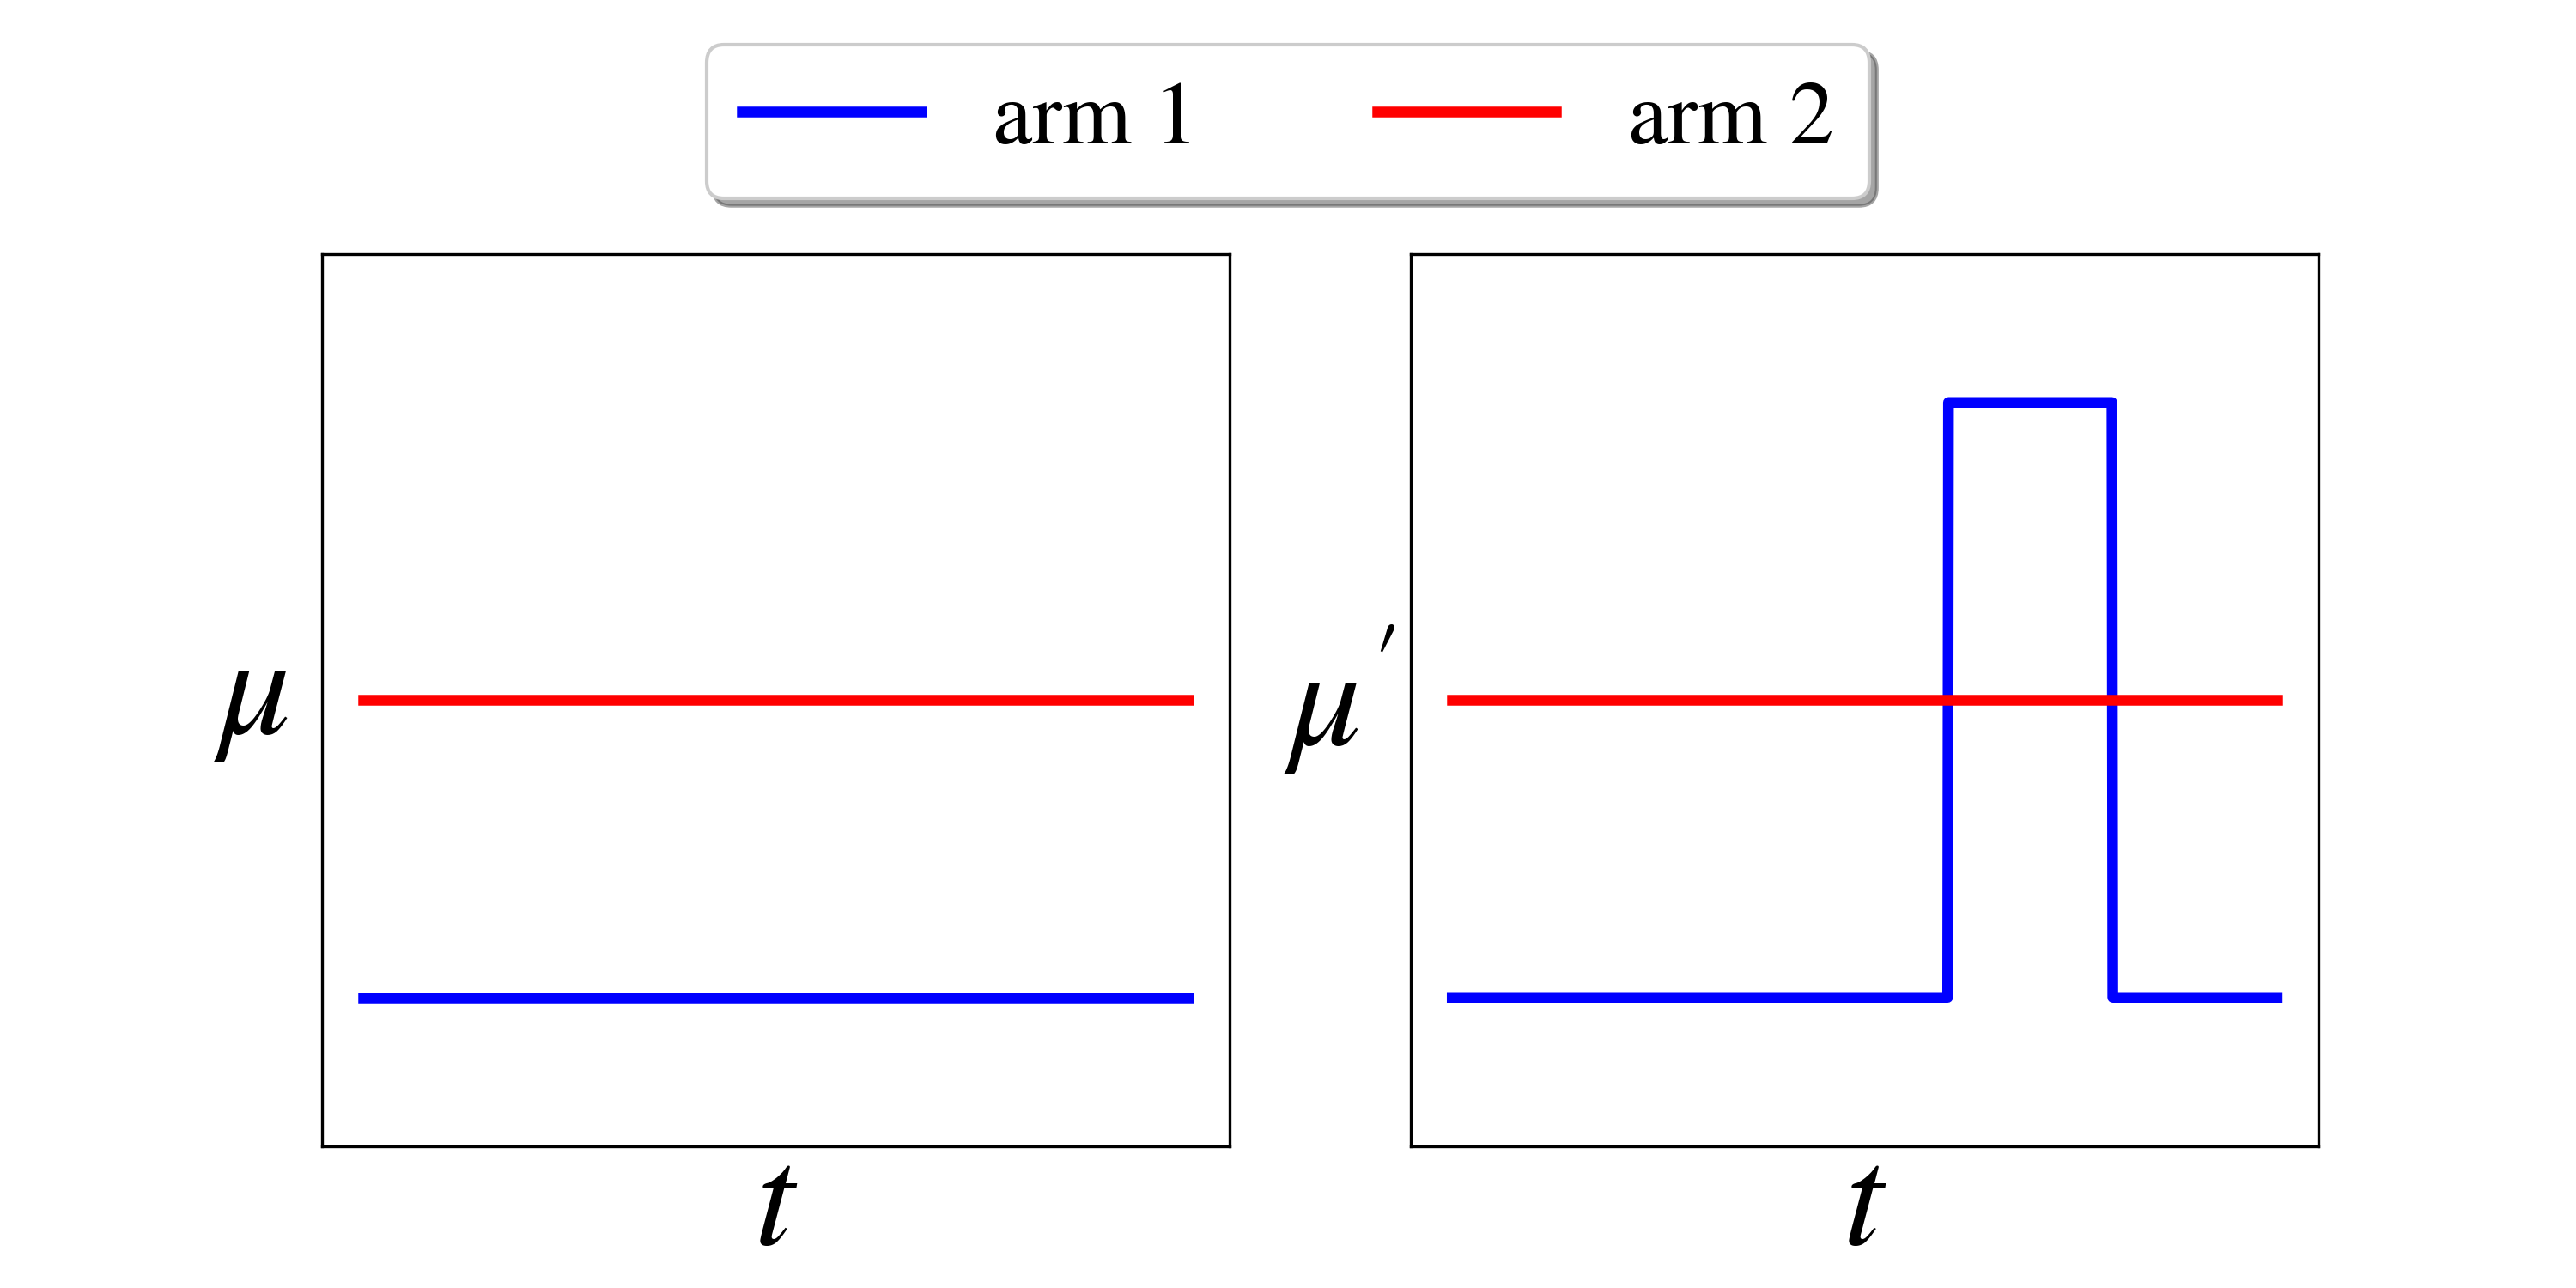
\includegraphics[clip, width= 0.99\textwidth]{4Restless/fig/garivier_lb.png}
\caption{The reward functions $\mu$ and $\mu'$. A policy with low regret on $\mu$ cannot achieve low regret on $\mu'$.}
\label{fig:garivier-lb}
\end{figure*}

\begin{proposition}[Theorem~31.2, \citet{lattimore2020banditbook}]
\label{prop:garivier-lb}
If a policy $\pi$ performs a regret $R_T(\pi, \mu)$ on a 2-arm stationary instance $\mu$, one can find a piece-wise stationary instance $\mu'$ with only two breakpoints such that, for a sufficiently long horizon $T$, the regret is lower bounded by 
\[\EE{R_T(\pi, \mu')} \geq \frac{T}{22R_T(\pi, \mu)}\,\cdot\]  
\end{proposition}

\begin{corollary}
\label{cor:garivier-lb}
Let $\pi$ a minimax optimal policy on the piece-wise stationary setups. Then, for a sufficiently large horizon $T$, there exists a universal constant $C$ such that for all the 2-arm stationary problems $\mu$, 
\[
\EE{R_T(\pi,\mu)} \geq C\sqrt{T}.
\]
\end{corollary}

These results state that one cannot have simultaneously a near-optimal problem-dependent regret rate $\cO\pa{\log{T}}$ on stationary instances and the minimax optimal piece-wise stationary rate $\cO\pa{\sqrt{T}}$. It is very different from the stationary case (or even with the rested rotting bandits presented in the last section) where some algorithms are shown to perform optimally both problem-dependent and problem-independent wise \citep{lattimore2018refining, menard2017klucb++}.

\subsubsection{Policies for piece-wise stationary bandits.}
\paragraph{Softmax policies.} For any sequence generated by an oblivious adversary, \EXPS \citep{auer2002nonstochastic} - an extension of \EXP - is guaranteed to achieve $\cO\pa{\sqrt{K\Upsilon_T T\log\pa{KT}}}$ regret against the best policy among the ones which change arms at most $\Upsilon_T -1$ times. The bound holds in the special case where the adversary generates the reward with noisy piece-wise stationary functions. In that case, the pseudo-regret definition is equivalent to the piece-wise stochastic regret defined in Equation~\ref{eq:restless-regret}. Indeed, the optimal policy is included in the set of $\cO\pa{\pa{KT}^{\Upsilon_T}}$ policies with at most $\Upsilon_T-1$ change of arms. 

\paragraph{Passive forgetting policies.} \DUCB \citep{kocsis2006discounted} and \SWUCB \citep{garivier2011upper-confidence-bound} are two ucb index policies which forget the older sample either by a discount factor or by a sliding window mechanism. The confidence interval increases when an arm has not been pulled for many rounds. When they are adequately tuned, these policies achieve respectively $\cO\pa{\sqrt{K\Upsilon_T T}\log{T}}$ and $\cO\pa{\sqrt{K\Upsilon_T T \log{T}}}$ minimax regret rate. While these policies do not improve the rate of \EXPS, they are deterministic and more explainable. 

\paragraph{Change-detection policies.} Instead of throwing away old samples at a fixed pace, one could remove samples from the index only when they notice a change in the arm's mean. This is the spirit of the Change-Detection ucb algorithms. These algorithms have three components: an ucb index, a change-detection subroutine, and a fixed active exploration rate (either deterministic or random pulls). The active exploration rate is meant to detect the arms which change from suboptimal value to optimal ones (like in Figure~\ref{fig:garivier-lb}). The optimal budget dedicated to active exploration scales with $\cO\pa{\sqrt{K\Upsilon_T T}}$. %When $\Upsilon_T$ is unknown, one can set a count $\Upsilon$ to $1$ and increases it at each detected change. 

\MUCB \citep{cao2019nearly} uses a simple change detector which compares the average of the last $\nicefrac{w}{2}$ samples with the average of the before last $\nicefrac{w}{2}$ ones and check whether the difference is significant or not. The optimal tuning of the parameter $w$ depends on the value of $\Upsilon_T$: if changes are large and frequent, one should choose a small value of $w$; if changes are small and sparse, one should choose a large value of $w$.

\CUSUMUCB \citep{liu2018change-detection} uses a change detector which constructs two random walks based on the upper and lower deviation of the new samples compared to the mean of the $M$ first ones. If one of the random walks reaches a threshold $h$, then the change detector triggers. The random walks are negatively biased with a small value $\epsilon$ to prevent the natural deviation to trigger the change detector. Again, the optimal value of the parameters $M$, $\epsilon$ and $h$ depends on the number of changes $\Upsilon_T$.

\GLRUCB \citep{besson2019generalized} uses the Gaussian Likelihood Ratio change detector. This change detector scans all the samples to detect any size of change on any period with high probability. The probability parameter only needs the knowledge of the horizon $T$ to achieve near-optimal minimax bound. \citet{mukherjee2019distribution} introduces a very similar algorithm but study the assumption where all the arms change their value significantly at each breakpoint. With this assumption, they do not need active exploration and recover problem-dependent bound $\cO\pa{\log{T}}$.

On the theoretical side, the analysis often assumes that each change is large enough to be detected before the next change. Indeed, after the detection of the breakpoint, they use the analysis of \UCB on each stationary batch. Before the change detection, they do not provide any non-trivial bound on the quality of the selected arm. 


\paragraph{Agnostic policies.}
\citet{auer2019adaptively} consider the problem with no assumption on the change-point detectability. They propose \ADSWITCH, which also uses a parameter-free change-detection subroutine but with an elimination policy: it pulls arms in a round-robin way a refined set of good arms. Arms are excluded from this set when they demonstrate with high probability that they underperform. The bad arms are also actively explored with consecutive sampling: the algorithm selects at random an arm and a deviation size $\Delta$ and pulls the arm the right number of rounds to detect if there is a change of size $\Delta$ in the arm's value. \citet{chen2019new} extend this technique to the contextual bandits problem.

A previous attempt \citep{cheung2019new} to solve this problem uses an expert aggregation bandit algorithm (e.g. \EXPfour) to select between different tuning of \SWUCB . Yet expert aggregation of bandit algorithm is problematic \citep{agarwal2017corralling, besson2018aggregation}, and \citet{cheung2019new} has to run each copy by batch with full restart. This technique leads to a suboptimal rate $\tcO\pa{\sqrt{K \max\pa{\Upsilon_T, \sqrt{T}} T}}$.


\subsection{Variation budget bandits}
\label{subsec:variation}
\citet{besbes2014stochastic} introduce the limited variation budget bandits, a restless setting where at each round Nature can modify the reward value of any arm but with a limited total variation budget $V_T$ at the round $T$. 

\begin{assumption}
\label{assum:variation}
$\mu_i : \NN^\star \rightarrow [- V_T, 0]$ are functions of the time $t$ with $V_T$ a positive constant. Moreover, we have that 
\begin{equation}
\label{eq:defbudget}
    \sum_{t=1}^{T-1} \sup_{i \in \arms} |\mu_i(t+1) - \mu_i(t) | \leq V_T\,.
\end{equation}
\end{assumption}


\paragraph{Lower Bound}
\begin{proposition}[\citet{besbes2014stochastic}]
\label{prop:variation_lb}
For any strategy $\pi$, there exists a  variation budget bandit scenario with means $\{\mu_i(t)\}_{i,t}$ satisfying Assumption~\ref{assum:variation} with a budget $V_T \geq \sigma \sqrt{\frac{K}{8T}}$ such that
%
\[
    \mathbb{E}\left[R_T(\pi)\right] \geq \frac{1}{16\sqrt{2}} \pa{\sigma^2 V_T KT^2}^{1/3}.
\]
\end{proposition}

In the next section, we prove a stronger statement, using only non-increasing reward functions. Yet, there is no additional difficulty. While the two Assumptions~\ref{assum:piece-wise} and~\ref{assum:variation} leads to different regret rate (see Proposition~\ref{prop:piecewise_lb}), the proof (see e.g. Lemma~\ref{lemma:lb} in the next subsection) shows that there is a strong similarity between the two problems, at least from a minimax perspective.

\paragraph{Policies for variation budget bandits.}
Most of the algorithms presented for the piece-wise stationary case are also near-optimal for the variation budget case. Indeed, \citet{besbes2014stochastic} show that \EXPS also learns in the variation budget setup. They also present \REXP, an algorithm based on \EXP with periodic restart which recovers a similar guarantee than \EXPS. \citet{cheung2019new} and \citet{russac2019weighted} extend \SWUCB and \DUCB to the linear bandit setting with variation budget. \citet{chen2019new} proves that \ADSWITCH is also optimal in the variation budget setting. However, change-detection ucb algorithms are not proved to perform well in the variation budget setting. Indeed, their proofs use the proof of \UCB on each stationary batch. In the variation budget setup, there is no stationary batch, which makes these algorithms harder to analyze. 

\subsection{The restless rotting assumption}
\label{subsec:restless-rotting}
\begin{assumption}
\label{assum:restless_rotting}
Reward functions $\left\{\mu_i \right\}_i$ are non-increasing with $t$.
\end{assumption}
We use this Assumption with Assumption~\ref{assum:piece-wise} and~\ref{assum:variation}.
\begin{remark}
\label{remark:budget}
With the rotting assumption, the variation budget assumption is very similar to the bounded assumption. Indeed, any set of decreasing functions $\mu_i : \NN^\star \rightarrow [- V, 0]$ satisfies Equation~\ref{eq:defbudget} with $V_T = KV$. Reciprocally, any set of functions satisfying Equation~\ref{eq:defbudget} with $\mu_i(1) \in [- V_T, 0]$ are bounded in $[- 2V_T, 0]$. 
\end{remark}

\paragraph{Lower bounds.} We show that our additional decreasing assumption does not change the minimax rates of the two settings. This is an adaptation of the proof of \citet{besbes2014stochastic} where we only use rotting functions.

\begin{restatable}{proposition}{restapiecewiselb}
\label{prop:piecewise_lb2}
For any strategy $\pi$, there exists a \underline{rotting} piece-wise stationary bandit scenario with means $\{\mu_i(t)\}_{i,t}$ \underline{satisfying Assumptions~\ref{assum:piece-wise} and~\ref{assum:restless_rotting}} with $\Upsilon_T\! \leq \!\pa{\!\frac{32V^2T }{K\sigma^2}\!}^{\!\nicefrac{1}{3}\!}\!$ such that,
\[
    \mathbb{E}\left[R_T(\pi)\right] \geq \frac{\sigma}{32}\sqrt{ \Upsilon_T KT}\,.
\]
\end{restatable}
\begin{restatable}{proposition}{restavariationlb}
\label{prop:variation_lb2}
For any strategy $\pi$, there exists a \underline{rotting} variation budget bandit scenario with means $\{\mu_i(t)\}_{i,t}$ \underline{satisfying Assumptions~\ref{assum:variation} and~\ref{assum:restless_rotting}} with a budget $V_T \geq \sigma \sqrt{\frac{K}{8T}}$ such that,
%
\[
    \mathbb{E}\left[R_T(\pi)\right] \geq \frac{1}{16\sqrt{2}} \pa{\sigma^2 V_T KT^2}^{\nicefrac{1}{3}}.
\]
\end{restatable}

The condition on $\Upsilon_T$ in Proposition~\ref{prop:piecewise_lb2} follows from Remark~\ref{remark:budget}: if $V$ is too small compared to $\Upsilon_T$, then we have a budget constraint - with associated lower bound in Proposition~\ref{prop:variation_lb2} - rather than a breakpoint constraint.


\paragraph{Proof}
 Our proof build a set of rotting piece-wise stationary problems with an evenly spaced set of $\Upsilon -1$ breakpoints. The adversary can choose the distance between arms $\Delta=\frac{1}{4} \sqrt{\frac{\sigma^{2} K \Upsilon}{2 T}}$ at the maximum such that the best arm is barely identifiable between two breakpoints (see Lemma~5.1, \citet{auer2002nonstochastic}). At each breakpoint, each arm's value decreases by $\Delta$ or $2\Delta$. Even if the set of breakpoints would be known, the learner does not know which arm is the best on each stationary part. Hence, in the worst case, she suffers at least the sum of the minimax regret of $\Upsilon$ stationary bandits problems with horizon $\frac{T}{\Upsilon}$, \textit{i.e.}  $\cO \pa{\sqrt{K\Upsilon T}}$. In the piece-wise stationary setting, we can simply identify $\Upsilon = \Upsilon_T$. In the variation budget setting, the adversary has a constraint over $\Upsilon \Delta = \frac{1}{4} \sqrt{\frac{\sigma^{2} K \Upsilon^3}{2 T}}=  \cO\pa{V_T}$. Hence, when the budget is limited, the adversary can choose up to $\Upsilon = \cO\pa{ T^{1/3}}$ breakpoints such that the suboptimal arms are "sufficiently" far from the best one (\textit{i.e} at $\Delta$). This dependence on $T$ leads to the increased regret rate of $\cO\pa{T^{\nicefrac{2}{3}}}$.
 
\begin{lemma}\label{lemma:lb}
Let $\Upsilon \in \left\{1,\dots, T\right\}$ and $\left\{\tau_k \triangleq \ceil{\frac{T}{ \Upsilon}} \text{ if } k \leq T \bmod{\Upsilon} \text{ else } \floor{\frac{T}{ \Upsilon}}\right\}_{k\leq \Upsilon}$. We call $t_k = \sum_{k'=1}^k \tau_{k'}$ and $t_0 = 0$.  Consider a family of piece-wise stationary bandits indexed by a vector $i^\star\in (\{0\}\cup \arms)^{\Upsilon}$ as follows: arm $i$ is a Gaussian distribution $\mathcal{N}\pa{\mu_i(t), \sigma}$ such that 
\[
\forall k \in \left\{0 , \dots, \Upsilon -1 \right\}, \ \forall t \in \left\{t_{k-1}+1,\dots, t_{k}\right\}, \ 
\mu_i(t) = 
\begin{cases}
-k \Delta \text{ if } i = i^\star_k\\
-(k+1)\Delta  \text{ else.}
\end{cases}
\]
We denote by $\EEempty_{i^\star}$ the expectation under the problem indexed by $i^\star$. Then, if $\Delta = \frac{1}{4}\sqrt{\frac{\sigma^2K\Upsilon}{2T}}$, for any policy $\pi$ :
\[
 \exists i^\star\in (\{0\}\cup \arms)^{\Upsilon}, \  \EEempty_{i^\star}\big[R_T(\pi)\big]  \geq  \frac{\sqrt{\sigma^2KT\Upsilon}}{32}\cdot
\]
\end{lemma}
\begin{proof}
Note that when $i^\star_k = 0$ then all the arms share the same means. We also define the vector $i^\star_{-k}$ equals to $i^\star$ with the coordinate $k$ empty and for $i\in\arms$ the vector $(i^\star_{-k},i)$ as the vector where we fill the empty coordinate with $i$.  We fix a policy $\pi$ and we will lower bound its average regret on the bandits problem indexed by $i^\star \in \arms^\Upsilon$ 
\begin{align*}
    \frac{1}{K^{\Upsilon}} \sum_{i^\star\in \arms^{\Upsilon}}  \EEempty_{i^\star}\big[R_T(\pi)\big] &= \frac{1}{K^{\Upsilon}} \sum_{i^\star\in \arms^{\Upsilon}} \sum_{k=1}^{\Upsilon}\Delta \EEempty_{i^\star}[\tau_k - N_{i^\star_k}^k] \\
    &=\Delta \left(T - \frac{1}{K^{\Upsilon}} \sum_{i^\star\in \arms^{\Upsilon}} \sum_{k=1}^{\Upsilon} \EEempty_{i^\star}[N_{i^\star_k}^k]\right),
\end{align*}
where $N_i^k$ is the number of pulls of arm $i$ during epoch $k$. Thus we need to upper bound the following quantity
\[
\frac{1}{K^{\Upsilon}} \sum_{i^\star\in \arms^{\Upsilon}} \sum_{k=1}^{\Upsilon} \EEempty_{i^\star}[N_{i^\star_k}^k] = \sum_{k=1}^{\Upsilon} \frac{1}{K^{\Upsilon-1}} \sum_{i^\star_{-k}\in \arms^{\Upsilon-1}}\frac{1}{K} \sum_{i=1}^K\EEempty_{(i^\star_{-k},i)}[N_{i}^k]\,.
\]
Using the contraction of the entropy for the bounded random variable $N_{i}^k/\tau_k$ then the Pinsker inequality (see \citet{garivier2018explore}) we get
\[
2\left(\frac{1}{\tau_k K} \sum_{i=1}^K\EEempty_{(i^\star_{-k},i)}[N_{i}^k] -\frac{1}{\tau_k K} \sum_{i=1}^K\EEempty_{(i^\star_{-k},0)}[N_{i}^k] \right)^2 \leq \frac{1}{K} \sum_{i=1}^K \EEempty_{(i^\star_{-k},0)}[N_{i}^k] \frac{\Delta^2}{2\sigma^2}\CommaBin
\]
since problems $(i^\star_{-k},i)$ and $(i^\star_{-k},0)$ differ only by a gap $\Delta$ on the arm $i$ during epoch $k$. Thanks to the fact that  $\sum_i N_i^k \leq \tau_k$ we get 
\[
\frac{1}{K} \sum_{i=1}^K\EEempty_{(i^\star_{-k},i)}[N_{i}^k] \leq \frac{\tau_k}{K} + \frac{\Delta}{2\sigma \sqrt{K}}\tau_k^{\nicefrac{3}{2}}\,.
\]
Putting all together we have for $K\geq 2$
\begin{align*}
    \frac{1}{K^{\Upsilon}} \sum_{i^\star\in \arms^{\Upsilon}}  \EEempty_{i^\star}\big[R_T(\pi)\big]  \geq \left(\frac{T}{2} -  \sum_{k=1}^{\Upsilon} \frac{\tau_k^{\nicefrac{3}{2}} \Delta}{2\sigma \sqrt{K}}\right)\Delta\,.
\end{align*}
We have $\tau_k= \floor{\frac{T}{\Upsilon}}$ or $\tau_k= \ceil{\frac{T}{\Upsilon}}$  such that $\sum_{k=1}^{\Upsilon} \tau_k=T$. Hence, we have that $\tau_k \leq 2T/\Upsilon$ which leads to 
\[
 \frac{1}{K^{\Upsilon}} \sum_{i^\star\in \arms^{\Upsilon}}  \EEempty_{i^\star}\big[R_T(\pi)\big]  \geq  \left(\frac{1}{2}T - \frac{\sqrt{2}T^{\nicefrac{3}{2}}\Delta}{\sigma \sqrt{K\Upsilon}}\right)\Delta\,.
\]

Choosing $\Delta = \frac{1}{4}\sqrt{\frac{\sigma^2K\Upsilon}{2T}}$, we get 
\[
 \frac{1}{K^{\Upsilon}} \sum_{i^\star\in \arms^{\Upsilon}}  \EEempty_{i^\star}\big[R_T(\pi)\big]  \geq  \frac{1}{4}\sqrt{\frac{\sigma^2K\Upsilon}{2T}}\left(\frac{1}{4}T\right) \geq \frac{\sqrt{\sigma^2KT\Upsilon}}{32}\cdot
\]
We can conclude by noticing that the average expected regret across the problem set is lesser or equal to the maximum across the same problem set.
\end{proof}
\restapiecewiselb*
\begin{proof}
This result directly follows from Lemma~\ref{lemma:lb} by choosing $\Upsilon = \Upsilon_T$. Indeed, the set of problems $\left\{i^\star \in \left(\left\{0\right\} \cup \arms\right)^{\Upsilon_T} \right\}$ satisfy Assumptions~\ref{assum:piece-wise} and~\ref{assum:restless_rotting} as soon as $\Upsilon_T\Delta \leq V$, \ie $\Upsilon_T \leq \pa{\frac{32V^2T }{K\sigma^2}}^{\nicefrac{1}{3}}$.
\end{proof}

\restavariationlb*
\begin{proof}
\sloppy
We want to use Lemma~\ref{lemma:lb} but we need to make the set of problems $\left\{i^\star \in \left(\left\{0\right\} \cup \arms\right)^{\Upsilon_T} \right\}$ comply with Assumption~\ref{assum:variation}. First, the function are bounded by $-V_T$. Hence, we need : 
\begin{equation}
\label{eq:bounded_condition}
  \Upsilon \Delta \leq V_T.  
\end{equation}

Second, the total variation is bounded according to Equation~\ref{eq:defbudget}. When $t$ is not a breakpoint, the variation is null. At each breakpoint, the maximal variation across the arm is $2\Delta$. For $\Upsilon-1$ breakpoint, we have that 


\begin{equation}
\label{eq:totalvar_condition}
  2\Delta \pa{\Upsilon-1}  \leq V_T.  
\end{equation}

Since $ 2\Delta \pa{\Upsilon-1} \leq \frac{\sigma}{2}\sqrt{\frac{K}{2T}}\Upsilon^{\nicefrac{3}{2}} $, we choose 
\begin{equation}
\label{eq:set_upsilon}
\Upsilon = \min\pa{\max\pa{\floor{ 2\left(\frac{V_T^{2}T}{K\sigma^{2}}\right)^{\nicefrac{1}{3}}},1},T}.
\end{equation}

By construction, \ref{eq:set_upsilon} satisfies \ref{eq:totalvar_condition}. Moreover, when $\Upsilon >1$, \ref{eq:totalvar_condition} is more restrictive than \ref{eq:bounded_condition}. For $\Upsilon = 1$, we simply assume $\Delta \leq V_T$, \textit{i.e.} $V_{T} \geq \sigma \sqrt{\frac{K}{8 T}}$.

Plugging \ref{eq:set_upsilon} in Lemma~\ref{lemma:lb} allows us to conclude 
\[
    \mathbb{E}\left[R_T(\pi)\right] \geq \frac{1}{16\sqrt{2}} V_T^{\nicefrac{1}{3}}\sigma^{\nicefrac{2}{3}}K^{\nicefrac{1}{3}}T^{\nicefrac{2}{3}}.
\]
\end{proof}
%!TEX root = ../main.tex
\section{Analysis of adaptive window policies on restless rotting bandits.} 
\label{sec:restless-theory}
In Chapter~\ref{ch:rested}, we presented four adaptive window policies (\FEWA, \RAWUCB, \EFFFEWA, \EFFRAW). The proof of the regret upper bounds in the rested case uses three main steps. First, we design one favorable event per round on which all the constructed statistics concentrate on a well-chosen confidence region, such that it holds with sufficiently high probability. This part does not use that we faced a rested non-stationary environment; it only uses the concentration of independent subgaussian variables which remains true in our restless problem (see Equation~\ref{eq:restless-feedback}). Hence, we restate Propositions~\ref{prop:prb_favorable_event} and~\ref{prop:prb_favorable_event_eff},
\begin{proposition}
\label{prop:prb_favorable_event_full}
We recall that, for any round $t$ and confidence $\delta_{t} \triangleq 2t^{-\alpha}$, we define
%
\begin{align*}
&\!\HPevent\! \triangleq\! \Big\{ \forall i\!\in\!\arms,\ \forall n \!\leq\! t\!-\!1 ,\ \forall h \!\leq\! n, \big| \hmu^h_i(t, \pi) - \bmu^h_i(t, \pi) \big| \!\leq\! c(h, \delta_{t}) \!\Big\}\\
&\!\HPeff\! \triangleq\! \Big\{ \forall i\!\in\!\arms, \forall n \!\leq\! t\!-\!1 , \forall h_j \!\in\! \Him(n), \big| \hmueff(t,\pi) - \bmueff(t,\pi) \big| \!\leq\! c(h_j, \delta_{t}) \!\Big\}
\end{align*}
with  $c(h,\delta_{t}) \triangleq \sqrt{2 \subgaussian^2\log(2/\delta_t)/h}$. Then, for a policy $\pi$ which pulls each arms once at the beginning, and for all $t>K$,
\[
\PPempty\Big[\bar{\HPevent}\Big] \leq \frac{Kt^2\delta_{t}}{2}=Kt^{2-\alpha} \text{ and } \PPempty\Big[\bar{\HPeff}\Big] \leq 3Kt\delta_t= 6Kt^{1-\alpha}.
\]
\end{proposition} 

Then, we use the mechanics of the algorithms to relate the average past performance of the selected arm with the current best value of the arms. As we noticed in the proofs (see e.g. the proof of Lemma~\ref{lem:core-FEWA}), we do not use the rested aspect of the problem. In fact, these results hold for a more general reward function $\mu_i(t,n)$ which is non-increasing with both $t$ and $n$. Therefore, we also restate Lemmas~\ref{lem:core-FEWA}, \ref{lem:core-RAWUCB} and~\ref{lem:core-eff},
\begin{lemma}
\label{lem:core-full}
At any round $t$ on favorable event $\HPevent$ (respectively, $\HPtwo$), if arm~$i_{t}$ is selected by $\pi \in \left\{\piF, \piR\right\}$ (respectively, $\pi \in \left\{\piEF, \piER\right\} $ tuned with $m=2$), for any $h \leq \Nitmone$,  the average of its $h$ last pulls cannot deviate significantly from the best available arm at that round, i.e.,
\begin{equation*}
\bmu^{h}_{i_t}(t,\pi) \geq \max_{i \in \arms} \mu_{i}(t)- \frac{C_\pi}{\sqrt{2\alpha}} c(h, \delta_t) \quad \text{with } 
\begin{cases}
C_{\piR} = 2\sqrt{2\alpha} \text{ and } C_{\piER} = \frac{4\sqrt{\alpha}}{\sqrt{2}-1}\\
C_{\piF} = 4\sqrt{2\alpha} \text{ and }C_{\piEF} = \frac{8\sqrt{\alpha}}{\sqrt{2}-1}
\end{cases}\cdot
\end{equation*}
\end{lemma}
Last, we use a specific rested regret decomposition to show that our algorithms are near-optimal both problem-dependent and problem-independent wise on rested rotting bandits. Unfortunately, this part cannot be used for the restless analysis. However, with a specific restless regret decomposition (see the proof in Subsection~\ref{ss:restless-proof}), we can show that our policies matches the two aforementioned lower bounds up to poly-logarithmic terms without any knowledge of the horizon $T$ nor $\Upsilon_T$ or $V_T$.
%
\begin{restatable}{theorem}{restapiecewisetheorem}
\label{th:piecewise-minimax}
Let $\pi \in \left\{ \piF, \piR\right\}$ tuned with $\alpha \geq 4$ or $\pi \in \left\{ \piEF, \piER\right\}$ tuned with $\alpha \geq 3$ and $m=2$. For any piece-wise stationary bandit scenario with means $\{\mu_i(t)\}_{i,t}$ satisfying Assumptions~\ref{assum:piece-wise} and~\ref{assum:restless_rotting}  with $\Upsilon_T-1$ change-points, $\pi$  suffers an expected regret\,
\[
\EE{R_T(\pi)} \leq C_\pi \sigma \sqrt{\log{T}} \pa{ \sqrt{\Upsilon_T KT} + \Upsilon_T K} + 6KV.
\]
\end{restatable}
\vspace{-2em}
\begin{restatable}{theorem}{restabudgettheorem}
\label{th:variation-minimax}
Let $\pi \in \left\{ \piF, \piR\right\}$ tuned with $\alpha \geq 4$ or $\pi \in \left\{ \piEF, \piER\right\}$ tuned with $\alpha \geq 3$ and $m=2$. For any variation budget bandit scenario with means $\{\mu_i(t)\}_{i,t}$ satisfying Assumptions~\ref{assum:variation} and~\ref{assum:restless_rotting}  with variation budget $V_T$, $\pi$ suffers an expected regret\,
\[
\mathbb{E}\left[R_T(\pi)\right] \leq 4\pa{C_\pi^2 \sigma^2 V_T K T^2\log{T}}^{\nicefrac{1}{3}} \!+ 2\Big(C_\pi \sigma V_T^2  K^2  T \sqrt{\log{T}}\Big)^{\nicefrac{1}{3}} \!+ 6 V_T K.
\]
\end{restatable}
%
The remaining terms are of second-order when $KV_T \leq \cO{\pa{T}}$, which is a necessary condition for the problem to be learnable (see Proposition~\ref{prop:variation_lb2}). 
%
\paragraph{Are rotting restless bandits easier?} Learning at the minimax rate without knowing $\Upsilon_T$ or $V_T$ was achieved in the non-rotting setup by significantly more complex algorithms. For instance, \citet{auer2019adaptively} use a combination of filtering on the set of potentially good arms, forced exploration planning on identified bad arms, and full restart of the algorithm when a change is detected. This algorithmic complexity has a performance cost, as \ADSWITCH is guaranteed to achieve 56 times the leading term in Theorem~\ref{th:piecewise-minimax}. Moreover, these algorithms rely on doubling trick when the horizon is unknown, which also has a regret cost compared to intrinsically anytime algorithms \citep{besson2018doubling}.

Yet, Proposition~\ref{prop:piecewise_lb2}  and~\ref{prop:variation_lb2} show that the rotting assumption do not improve the minimax rate for the two considered setups. Interestingly both these lower bounds are matched by (tuned) \EXPS \citep{auer2002nonstochastic}, an algorithm originally designed for switching best arm in adversarial sequences of rewards. This is comparable to the fixed best arm world:  adversarial and stochastic bandits share the same minimax rate which is matched in both setups by \EXP. The main interest of the stochastic assumption is to allow for \textit{problem dependent analysis}. For the stochastic stationary bandits, it leads to a stronger $\cO{\pa{\log\pa{T}}}$ bounds. In the (non-rotting) piece-wise stationary setting, we argued in Subsection~\ref{subsec:piecewise} that the learner has to maintain $\cO\pa{\sqrt{T}}$ exploratory pulls to shield against increase of currently suboptimal arm (see Proposition~\ref{prop:garivier-lb} and Corollary~\ref{cor:garivier-lb}).

The decreasing Assumption~\ref{assum:restless_rotting} excludes the problems where suboptimal arms increases to become optimal from the set of possible problems. Theorem~\ref{th:piecewise_pd} shows that not only \RAWUCB is able to recover the $\cO\pa{\log\pa{T}}$ on stationary problems but also recovers the same rate on each batch of a rotting piece-wise stationary problem. 
\begin{restatable}{theorem}{restapiecewisetheorempd}
\label{th:piecewise_pd}
Let $\pi \in \left\{ \piF, \piR\right\}$ tuned with $\alpha \geq 4$ or $\pi \in \left\{ \piEF, \piER\right\}$ tuned with $\alpha \geq 3$ and $m=2$. For any piece-wise stationary bandit scenario with means $\{\mu_i(t)\}_{i,t}$ satisfying Assumptions~\ref{assum:piece-wise} and~\ref{assum:restless_rotting}  with $\Upsilon_T-1$ change-points, $\pi$ suffers an expected regret\,
\[
    \mathbb{E}\left[R_T(\pi)\right] \leq \sum_{k=0}^{\Upsilon_T-1} \sum_{i\in\arms} \frac{C_\pi^2 \sigma^2\log{T}}{\Delta_{i,k}} +  C_\pi \sigma \Upsilon_T K \sqrt{ \log{T}} + 6KV. 
\]
\end{restatable}
%TODO talk about tuning ?
%When $\Upsilon_T = 1$ (no changepoint), \RAWUCB recovers the same guarantee than \UCBone. However, \UCB with a more careful tuning $\delta_t \sim \frac{1}{t\log{t}^2}$ match \citet{lai1985asymptotically} asymptotic factor for Gaussian bandits \citep{lattimore2019bandit}. We leave the two following questions for future analysis: 1) Is there a tuning of $\delta_t$ such that \RAWUCB is asymptotic for stationary problems? 2) If yes, can \RAWUCB with this asymptotic tuning recovers some (rested or restless) non-stationary guarantees?

Notice that \citet{mukherjee2019distribution} use a different assumption to recover a similar problem-dependent bound. Indeed, they assume that all the arms change at the same time which also excludes $\mu'$ from the set of possible problems. %TODO
%Therefore, \RAWUCB is near minimax optimal \emph{and} reaches the asymptotic rate for stationary bandits $O(\sum_{i \in \arms} \frac{\log(T)}{\Delta_i})$ (see Corollary~\ref{dependent_theorem}) without knowing the number of change points nor the horizon. 

\subsection{Proofs}
\label{ss:restless-proof}

\subsubsection*{Sketch.} 

We start by separating the regret on the bad events $\bar{\HPevent}$ from the good events $\HPevent$. According to Proposition~\ref{prop:prb_favorable_event}, the bad events $\bar{\xi}_t$ have low probability for appropriate $\alpha$. For $\alpha = 4$, they weigh at most $\cO{\pa{KV}}$ in the expected regret.  On the good events, we write:
\vspace{-4pt}
\begin{equation}
\label{eq:restless-regret-decompo}
R_T(\pi)= \sum_{t=1}^T \mu_{i_t^\star}(t) - \bar{\mu}_{i_t}^{h_t}(t, \pi) + \bar{\mu}_{i_t}^{h_t}(t, \pi) - \mu_{i_t}(t).   
\end{equation}

Notice that Lemma~\ref{lem:core-full} can bound the first difference for any $h_t$. When the reward is piece-wise stationary, we can select $h_t$ such that we include all the pulls of arm $i_t$ from the current stationary batch. If there is none, then it is the first pull of arm $i_t$ in this batch. We handle these $\cO{\pa{K\Upsilon_T}}$ rounds separately (see Lemma~\ref{lem:FP}). In the other cases, we note that the second difference is null because $\bar{\mu}_{i_t}^{h_t}(t, \pi) = \mu_{i_t}(t) = \mu_i^k$ by the piece-wise stationary assumption. The remaining of the proofs of Theorem~\ref{th:piecewise-minimax} and~\ref{th:piecewise_pd} are then very similar to the analysis of \cite{auer2002finite} on each stationary batch. Indeed, Lemma~\ref{lem:core-full} is similar to the two confidence bounds guarantee of \UCBone's guarantee.

In the variation budget setting, there is no stationary batches. Hence, we cannot choose an $h_t$ which cancels the second difference in Equation~\ref{eq:restless-regret-decompo}. Yet, we still decompose the rounds in $\Upsilon$ batches of equal length for the analysis. We choose $h_t$ such that we include all the pulls of arm $i_t$ from the current batch. For the sum of the first differences in Equation~\ref{eq:restless-regret-decompo}, there is no difference with the piece-wise stationary case and we can bound
\vspace{-4pt}
\begin{equation}
\label{eq:variance_bound}
    \sum_{t=1}^T \mu_{i_t^\star}(t) - \bar{\mu}_{i_t}^{h_t}(t, \pi)\leq \tcO{\pa{\sqrt{K\Upsilon T}}}.
\end{equation}
We call $\Delta_i^k \triangleq \mu_i(t_k) - \mu_i(t_{k+1})$, the total variation of arm $i$ in batch $k$. The sum of second differences in Equation~\ref{eq:restless-regret-decompo} can be bounded as follows: on each batch of $T\Upsilon^{-1}$ rounds, each second difference is bounded by $\max_{i\in \arms} \Delta_i^k$. When we sum over the batches, we get
\vspace{-4pt}
\begin{equation}
\label{eq:bias_bound}
  \sum_{t=1}^T  \bar{\mu}_{i_t}^{h_t}(t, \pi) - \mu_{i_t}(t)\leq \frac{T}{\Upsilon}\sum_{k=0}^{\Upsilon-1}\max_{i \in \arms}\Delta_i^k  \leq \frac{TV_T}{\Upsilon}\, .  
\end{equation}
Indeed, in the middle term, we have a maximum on the summed variation of arm $i$ in batch $k$. On the right-hand side, we have $V_T$ which bounds the sum over the rounds of maximal variation of the arms (see Equation~\ref{eq:defbudget}). Thus, the right-hand side is larger because the maximum of sums is smaller than the sum of maximums. We can then choose $\Upsilon = \tcO{\pa{T^{\nicefrac{1}{3}}V_T^{\nicefrac{2}{3}}K^{\nicefrac{-1}{3}}}}$ to minimise the sum of Equations~\ref{eq:variance_bound} and ~\ref{eq:bias_bound}. It leads to the leading term of our Theorem~\ref{th:variation-minimax}. Notice that we still have to handle the first pull of each arm in each batch. If we bound roughly each first pull by $V_T$, we would get $K\Upsilon V_T \sim \tcO{\pa{V_T^{\nicefrac{5}{3}}}}$ which would be the leading term for large $V_T$. Our Lemma~\ref{lem:FP} is more careful such that it leads to a second order term when $KV_T \leq o\pa{T}$.

\subsubsection*{Full proof}
\begin{lemma}[Bound on unfavorable events. Decomposition in unspecified batches. Bound on the first pull of each arm in each batch] %TODO
\label{lem:FP}
Let an integer $\Upsilon \in\left\{ 1, \dots,T\right\}$.\\
Let $\mu_i : \NN^\star \rightarrow \left[0, -V\right]$, the $K$ decreasing reward functions.\\ 
Let $\left\{t_k\in\left\{ 1, \dots,T\right\} \right.\allowbreak\left. |\, t_k > t_{k-1}\right\}_{k\in \left\{ 1, \dots,\Upsilon-1\right\}}$ a set of $\Upsilon - 1$ distinct rounds delimiting $\Upsilon$ batches. We set $t_0=0$ and $t_\Upsilon = T$. \\
We call $h_{i}^{k} \triangleq \sum_{t=t_k +1}^{t_{k+1}} \mathbbm{1}\left(i_{t} = i\right)$ the number of pulls of arm $i$ in batch $k$ and $t_i^k(h)$ the time at which arm $i$ is pulled for the $h$-th time since $t_k + 1$. We also call $\arms_k \triangleq  \left\{ i \in \arms | h_i^k \geq 1\right\}$ the set of pulled arms in batch $k$. 

Then, $\pi \in \left\{\piR, \piF \right\}$ run with $\alpha \geq 4$, or $\pi \in \left\{\piER, \piEF \right\}$ run with $m=2$ and $\alpha \geq 3$, suffers an expected regret of
\begin{align*}
\EE{R_T(\pi)} \leq &  \, \EE{\sum_{k=0}^{\Upsilon-1} \sum_{i\in\arms_k}\sum_{t=t_k +1 }^{t_{k+1}}\sum_{h=2}^{h^k_{i}}\mathbbm{1}\pa{ t = t_i^k(h) \land \HPevent} \Big(\mu_{\star}(t) - \mu_{i}(t)\Big)} \\
&+   C_\pi \sigma \Upsilon K\sqrt{\log{T}} + 6KV.
\end{align*}
\end{lemma}
\begin{proof}
We start by separating the favorable events from the unfavorable events:
\begin{equation}
\label{eq:event_sep}
    R_T(\pi) = \underbrace{\sum_{t=1}^T \mathbbm{1}\pa{\HPevent} \pa{\mu_{\star}(t) - \mu_{i_t}(t)}}_{R_T(\pi | \HPevent)} + \underbrace{\sum_{t=1}^T \mathbbm{1}\big(\bar{\HPevent}\big) \pa{\mu_{\star}(t) - \mu_{i_t}(t)}}_{{R_T(\pi | \bar{\HPevent})}} \,,
\end{equation}
with $\mu_\star(t) \triangleq \max_{i\in\arms}\mu_i(t)$. For $\alpha \geq 4$, we can bound the cost of the unfavorable events thanks to Proposition~\ref{prop:prb_favorable_event_full},
\begin{equation}
\label{eq:bad_event}
    \EE {R_T(\pi | \bar{\HPevent})} \leq \sum_{t=1}^T \PP{\bar{\HPevent}} V  \leq \sum_{t=1}^T \frac{KV}{t^2} = \frac{KV\pi^2}{6} \leq 2KV.
\end{equation}

On the favorable events, given any ordered set of $\Upsilon -1$ breakpoints $\left\{t_k\right\}$, we divide the horizon in $\Upsilon$ batches $\left\{t_k+1, \dots, t_{k+1} \right\}_{k \leq \Upsilon-1}$, 
\[
R_T(\pi | \HPevent) \leq \sum_{k=0}^{\Upsilon-1} \sum_{t=t_{k} +1 }^{t_{k+1}} \mathbbm{1}\pa{\HPevent} \big(\mu_{\star}(t) - \mu_{i_t}(t)\big).
\]
We define $h_{i}^{k}$ the number of pulls of arm $i$ in batch $k$, \textit{i.e.}  $h_{i}^{k} = \sum_{t=t_k +1}^{t_{k+1}} \mathbbm{1}\left(i_{t} = i\right)$. We use $t_i^k(h)$ to designate the time at which arm $i$ is pulled for the $h$-th time since $t_k$.
\[
R_T(\pi | \HPevent) \leq \sum_{k=0}^{\Upsilon-1} \sum_{t=t_k +1 }^{t_{k+1}} \sum_{i\in\arms_k} \sum_{h=1}^{h^k_{i}} \mathbbm{1}\pa{t_i^k(h) = t \land \HPevent} \Big(\mu_{\star}(t) - \mu_{i}(t)\Big).
\]
We split the regret on the first pulls of each batch,
\begin{align}
\label{eq:fp_op}
\begin{split}
    R_T(\pi | \HPevent) = & \underbrace{\sum_{k=0}^{\Upsilon-1}\sum_{t=t_{k} +1 }^{t_{k+1}} \sum_{i\in\arms_k} \mathbbm{1}\pa{t = t_i^k(1) \land \HPevent}\Big(\mu_{\star}(t) - \mu_{i}(t)\Big)}_{FP} \\ & +  \underbrace{\sum_{k=0}^{\Upsilon-1}\sum_{t=t_{k} +1 }^{t_{k+1}} \sum_{i\in\arms_k} \sum_{h=2}^{h^k_{i}}\mathbbm{1}\left( t = t_i^k(h) \land \HPevent \right)\Big( \mu_{\star}(t) - \mu_{i}(t)\Big)}_{OP} .
\end{split}
\end{align}

\paragraph{Analysis of the first pulls.}

We call $k_i^1$, the index of the batch at which arm $i$ is pulled for the first time.  We call $\arms_k^2 \triangleq \left\{ i \in \arms_k | k > k_i^1\right\}$, the set of arms pulled at least once during batch $k$ and at least once in a batch before $k$. We split the regret due to the very first pull each arm from the other first pulls in each batch,
\begin{align*}
FP  = &\sum_{k=0}^{\Upsilon-1}\sum_{i\in\arms_k}\sum_{t=t_{k} +1 }^{t_{k+1}}  \mathbbm{1}\pa{ t = t_i^k(1) \land \HPevent}\Big(\mu_{\star}(t) - \mu_{i}(t)\Big)\\
\leq& \sum_{i \in \arms}  \Big(0- \mu_i(t_i^{k_i^1}(1))\Big) +  \sum_{k=1}^{\Upsilon -1} \sum_{i\in \arms_k^2}\sum_{t=t_k +1 }^{t_{k+1}}  \mathbbm{1}\pa{t = t_i^k(1) \land \HPevent}\Big(\mu_{\star}(t) - \mu_{i}(t)\Big)\\
 =& \sum_{i \in \arms} \Big(0- \mu_i(t_i^{k_i^1}(1))\Big) \\
& + \sum_{k=1}^{\Upsilon -1} \sum_{i\in \arms_k^2} \sum_{t=t_k +1 }^{t_{k+1}}  \mathbbm{1}\pa{ t = t_i^k(1) \land \HPevent}\Big(\mu_{\star}(t) - \bar{\mu}^1_i(t, \pi) + \bar{\mu}^1_i(t,\pi) - \mu_{i}(t)\Big).
\end{align*}

The inequality is justified because $\mu_i(t) \leq 0$ for all $t$. In the last equation, we simply introduce $\bar{\mu}^1_i(t,\pi)$, the last pulled sample of arm $i$, which is well defined after the first pull of each arm.
According to Lemma~\ref{lem:core-full}, the first difference is bounded on the high-probability event $\HPevent$,
\begin{equation}
    \label{eq:fp_lemma1}
    \sum_{t=t_k +1 }^{t_{k+1}} \mathbbm{1}\pa{t = t_i^k(1) \land \HPevent}\pa{\mu_{\star}(t) - \bar{\mu}^1_i(t, \pi)} \leq \frac{C_\pi}{\sqrt{2\alpha}} c(1,2T^{-\alpha}) = C_{\pi} \sigma \sqrt{\log{T}}.
\end{equation}


We will show that we can telescope the second sum. First, we notice that we can collapse the sum on $t$ using $ \mathbbm{1}\pa{t = t_i^k(1)}$. Moreover, $\HPevent$ will not be needed: hence we can drop $\mathbbm{1}\pa{\HPevent} \leq 1 $.
\begin{equation}
\label{eq:fp_collapse}
 \sum_{t=t_k +1 }^{t_{k+1}} \mathbbm{1}\pa{ t = t_i^k(1) \land \HPevent}\pa{\bar{\mu}^1_i(t,\pi) - \mu_{i}(t)} \leq \bar{\mu}^1_i(t_i^k(1), \pi) - \mu_{i}(t_i^k(1)).
\end{equation}

For a given batch $k$ on which arm $i$ is pulled, the precedent reward sample has a mean $\bar{\mu}_i^h\pa{t_i^k\pa{1}, \pi}$. This sample is the last pull of the last batch $k'$ before $k$ on which arm $i$ is pulled. Hence, its mean is smaller than the mean of the first pull on this same batch $k'$ because the reward is decreasing. Hence, the sum can telescope
\begin{align}
\label{eq:fp_telescoping} 
\sum_{i \in \arms} \Big(0 -& \mu_i(t_i^{k_i^1}(1))\Big) + \sum_{k=1}^{\Upsilon -1}  \sum_{i\in \arms_k^2} \sum_{t=t_k +1 }^{t_{k+1}}\mathbbm{1}\pa{ t = t_i^k(1) \land \HPevent}\pa{ \bar{\mu}^1_i(t,\pi) - \mu_{i}(t)} \nonumber\\
& \leq \sum_{i \in \arms}\left\{ 0- \mu_i(t_i^{k_i^1}(1)) + \sum_{k=k_i^1 + 1}^{\Upsilon-1 } \mathbbm{1}\pa{h^k_{i} \geq 1  }\pa{\bar{\mu}^1_i(t_i^k(1), \pi) - \mu_{i}(t_i^k(1))} \right\} \nonumber\\
& \leq \sum_{i \in \arms} \Big(0-\mu_i(T)\Big) \leq KV\,.  
\end{align}
The first inequality uses the definition of $\arms_k^2$ along with Equation~\ref{eq:fp_collapse}. The second inequality follows from the telescoping argument presented above. The third inequality uses that $\mu_i(T) \geq -V$. Gathering Equation~\ref{eq:fp_lemma1} and  ~\ref{eq:fp_telescoping}, we can bound the term $FP$ (defined in Equation~\ref{eq:fp_op}) 
\begin{equation}
\label{eq:fp_bound}
FP \leq  KV + \sum_{k=1}^{\Upsilon - 1} \sum_{i\in \arms_k^2} C_\pi \sigma \sqrt{\log{T}} \leq KV + C_\pi \sigma \Upsilon K\sqrt{\log{T}} .    
\end{equation}



\paragraph{Conclusion.} From Equation~\ref{eq:event_sep}, we can bound the expected regret on the unfavorable events thanks to Equation~\ref{eq:bad_event}. On the favorable events, we can split the rounds in batches on which we isolate the first pull of each arm on each batch thanks to Equation~\ref{eq:fp_op}. Finally, we bound the regret due to these first pulls thanks to Equation~\ref{eq:fp_bound}, and for $\alpha \geq 4$,
\begin{align*}
\EE{R_T(\pi)} \leq &  \, \EE{\sum_{k=0}^{\Upsilon-1} \sum_{i\in\arms_k}\sum_{t=t_k +1 }^{t_{k+1}}\sum_{h=2}^{h^k_{i}}\mathbbm{1}\pa{ t = t_i^k(h) \land \HPevent} \Big( \mu_{\star}(t) - \mu_{i}(t)\Big)} \\
&+  C_\pi \sigma \Upsilon K \sqrt{\log{T}} + 3KV.
\end{align*}

For the efficient algorithms, we can use the same proof with $\HPtwo$ and get for $\alpha \geq 3$, 
\begin{align*}
\EE{R_T(\pi)} \leq &  \, \EE{\sum_{k=0}^{\Upsilon-1} \sum_{i\in\arms_k}\sum_{t=t_k +1 }^{t_{k+1}}\sum_{h=2}^{h^k_{i}}\mathbbm{1}\pa{ t = t_i^k(h) \land \HPevent} \Big(  \mu_{\star}(t) - \mu_{i}(t)\Big)} \\
&+  C_\pi \sigma \Upsilon K \sqrt{\log{T}} + 6KV.
\end{align*}

\end{proof}

\begin{lemma}[Analysis of the second pulls in each batch under the favorable events.]\label{lem:OP}
Let $\Delta_i^k \triangleq \mu_i(t_k+1) - \mu_i(t_{k+1})$, the decrement of arm $i$ in batch $k$. For any arm $i$ and any consecutive rounds $\left\{t_k+1, \dots , t_{k+1}\right\}$ such that $i$ is pulled $h_i^{k} \geq 1$ times, the regret due to the pulls after the first one can be bounded under the favorable events, 
\begin{multline*}
\sum_{t=t_{k} +1 }^{t_{k+1}} \sum_{h=2}^{h^k_{i}}\mathbbm{1}\left(t = t_i^k(h) \land \HPevent \right)\Big(  \mu_{\star}(t) - \mu_{i}(t)\Big) \\ \leq  \pa{h_i^k-1}\Delta_i^k + \sum_{h=2}^{h^k_{i}}\mathbbm{1}\left(\HPt{t_i^k(h)}\right)\pa{  \mu_{\star}(t_i^k(h)) - \bar{\mu}_i^{h-1}(t_i^k(h),\pi)} .
\end{multline*}
\end{lemma}
\begin{proof}
We call $\Delta_{i}(t,t')\triangleq \mu_i(t) - \mu_i(t')$ the variation of arm $i$ between times $t$ and $t'$.
As a short notation, we refer to $\Delta_i^k \triangleq \Delta_{i}(t_k+1,t_{k+1})$ for the variation of arm $i$ in batch $k$.

\begin{equation}
\label{eq:batch_delta_var}
    \forall h\leq h_i^k, \quad \mu_i( t_i^k(h)) \geq \mu_i(t_{k+1}) =  \mu_i(t_k +1 ) - \Delta_i^k \geq \bar{\mu}_i^{h-1}( t_i^k(h), \pi) - \Delta_i^k\,.
\end{equation} 
The two inequalities are justified by the rewards decay. Indeed, any pull in batch $k$ has a higher reward than the value of arm $i$ at the end of the batch $t_{k+1}$. Moreover, the value at the beginning of the batch is higher that any average of $h$ value in this batch. The middle equality follows from the definition of $\Delta_i^k$.

Then, we plug Equation~\ref{eq:batch_delta_var} in the left hand side of our claim,
\begin{align*}
\sum_{t=t_{k} +1 }^{t_{k+1}}
\sum_{h=2}^{h^k_{i}}\mathbbm{1}&\left(t = t_i^k(h) \land \HPevent\right)\Big(  \mu_{\star}(t) - \mu_{i}(t) \Big) \\
& = \sum_{h=2}^{h^k_{i}}\mathbbm{1}\left(\HPt{t_i^k(h)}\right)\pa{  \mu_{\star}(t_i^k(h)) - \mu_{i}(t_i^k(h))} \\
&\leq \sum_{h=2}^{h^k_{i}}\mathbbm{1}\left(\HPt{t_i^k(h)}\right)\pa{  \mu_{\star}(t_i^k(h)) - \bar{\mu}_i^{h-1}( t_i^k(h),\pi) + \Delta_i^k}\\
&\leq  \pa{h_i^k-1}\Delta_i^k + \sum_{h=2}^{h^k_{i}}\mathbbm{1}\left(\HPt{t_i^k(h)}\right)\pa{  \mu_{\star}(t_i^k(h)) - \bar{\mu}_i^{h-1}(t_i^k(h),\pi)} .
\end{align*}
The last inequality is justified by $\mathbbm{1}\left(\HPt{t_i^k(h)}\right)\leq 1$.
\end{proof}

\subsubsection*{Piecewise stationary rotting bandits.}
\sloppy
Let $\left\{t_k\right\}_{\left\{k \leq \Upsilon_T\right\}}$ be the set of breakpoints with $t_0=0$ and $t_{\Upsilon_T} = T$. For all $t \in \left\{t_k\! +\!1 , \dots , t_{k\!+\!1}\right\}$, $\mu_i(t) = \mu_i^k$. We denote $i^\star_k \in \argmax_{i\in \arms} \mu_i^k$ (one of) the best arm(s) in batch $k$, and $\mu_{\star}^k \triangleq \max_{i\in \arms} \mu_i^k$, the corresponding best value. We also call $\Delta_{i,k} \triangleq \mu_{\star}^k - \mu_i^k$ the gap between arm $i$ and optimal arm in batch $k$.

\begin{lemma}
\label{lem:OP-piecewise}
For an arm $i$ and a stationary batch $k$, we call $h_{i,\xi}^k \triangleq \max\left(h \leq h_i^k | \HPt{t_i^k(h)} \right)$ the last pull of arm $i$ in batch $k$ under the favorable events (possibly 0). If $h_{i,\xi}^k \geq 1$, the regret due to the second pulls on the favorable events is bounded by,
\[
\sum_{t=t_{k}+1}^{t_{k+1}} \sum_{h=2}^{h_{i}^{k}} \!\mathbbm{1}\!\pa{\! t=t_{i}^{k}(h) \land \HPevent \!}\!\Big(\!\mu_{\star}(t)\!-\!\mu_{i}(t)\!\Big) \leq\pa{\!h_{i, \xi}^{k}\!-\!1 \!} \Delta_{i, k} \leq C_\pi\sigma \sqrt{\pa{\!h_{i,\xi}^k\!-\!1\!}\log{T}}.
\]
\end{lemma}
\begin{proof}
We apply Lemma~\ref{lem:OP} on each stationary batch. Hence, $\Delta_i^k =0$ and we can write,
%
\begin{equation*}
\!\sum_{t=t_{k} +1 }^{t_{k+1}}\! \sum_{h=2}^{h^k_{i}} \! \mathbbm{1}\left(\!t = t_i^k(h) \land \HPevent \!\right)\Big(\! \mu_{\star}(t) - \mu_{i}(t)\!\Big) \leq   \sum_{h=2}^{h^k_{i}} \!\mathbbm{1}\left(\!\HPt{t_i^k(h)}\!\right)\pa{\!  \mu_{\star}(t_i^k(h)) - \bar{\mu}_i^{h-1}(t_i^k(h),\pi)\!}\! .
\end{equation*}

We notice that $\mu_{\star}(t_i^k(h)) = \mu_{\star}^{(k)}$. We call $h_{i,\xi}^k \triangleq \max\left(h \leq h_i^k\, \,| \HPt{t_i^k(h)} \right)$. Hence,
\begin{align*}
\sum_{h=2}^{h^k_{i}}\!\mathbbm{1}\left(\HPt{t_i^k(h)}\right)\!\pa{ \! \mu_{\star}(t_i^k(h)) \!-\! \bar{\mu}_i^{h\!-\!1}(t_i^k(h),\pi)\!}  & \!=\! \sum_{h=2}^{h^k_{i,\xi}}\!\mathbbm{1}\left(\HPt{t_i^k(h)}\right)\!\pa{  \mu^k_{\star} \!-\! \bar{\mu}_i^{h\!-\!1}(t_i^k(h), \pi)} \\
 &\leq \sum_{h=2}^{h^k_{i, \xi}} \mu_{\star}^{k} - \bar{\mu}_i^{h-1}(t_i^k(h), \pi)\\
 &= \sum_{h=2}^{h^k_{i, \xi}} \mu_{\star}^{k} - \mu_i^k\\
 & = \pa{h_{i,\xi}^k - 1 }\Delta_{i,k}\, .  
\end{align*}

The first equality follows from $\forall h > h_{i,\xi}^k, \, \mathbbm{1}\left(\HPt{t_i^k(h)}\right) =0$ by definition of $h_{i,\xi}^k$. The first inequality follows by dropping $\mathbbm{1}\left(\HPt{t_i^k(h)}\right) \leq 1$. The second equality uses that the function is stationary in batch $k$ : $\forall h \leq h_{i,\xi}^k, \bar{\mu}_i^{h-1}(t_i^k(h), \pi) = \mu_{i}^k.$ The last equality follows by definition of $\Delta_{i,k}$ (which does not depend on the summand index $h$).

Then, we apply Lemma~\ref{lem:core-full} at time $t_i^k\pa{h_{i,\xi}^k}$. By definition of $h_{i,\xi}^k$, $\mathbbm{1}\!\left(\!\HPt{t_i^k(h_{i,\xi}^k)\!}\right) = 1$.
\begin{align*}
 \pa{h_{i,\xi}^k - 1 }\Delta_{i,k}  \leq \frac{C_\pi}{\sqrt{2\alpha}}\pa{h_{i,\xi}^k - 1 }c(h_{i,\xi}^k\!-\!1, 2T^{-\alpha}) = C_\pi \sigma \sqrt{\pa{h_{i,\xi}^k-1}\log{T}}.
\end{align*} 
\end{proof}

\restapiecewisetheorem*
\begin{proof}

We apply Lemma~\ref{lem:OP-piecewise},
\[\sum_{k=0}^{\Upsilon_T-1} \! \sum_{i \in \mathcal{K}_{k}} \!\sum_{t=t_{k}+1}^{t_{k+1}} \! \sum_{h=2}^{h_{i}^{k}} \!\mathbbm{1}\!\left( \!t\!=\!t_{i}^{k}(h)\!\land\!\HPevent\!\right)\Big(\mu_{\star}(t)\!-\!\mu_{i}(t)\Big) \leq  \sum_{k=0}^{\Upsilon_T-1} \!\sum_{i\in\arms_k}\!  C_\pi \sigma \sqrt{h_{i,\xi}^k\log{T}} .\]

We notice that $ \sum_{k=0}^{\Upsilon_T -1}\sum_{i\in\arms_k} h_{i,\xi}^k\leq T$. Hence, thanks to Jensen's inequality, 
\[
\sum_{k=0}^{\Upsilon_T-1} \sum_{i\in\arms_k} C_\pi\sigma \sqrt{h_{i,\xi}^k\log{T}} \leq  C_\pi \sigma \sqrt{ \Upsilon_T K T\log{T}}.
\]

We use Lemma~\ref{lem:FP} with the last equation and conclude,
\[
\EE{R_T(\pi)} \leq C_\pi \sigma \sqrt{\log{T}} \pa{ \sqrt{\Upsilon_T KT} + \Upsilon_T K} + 6KV.
\]
\end{proof}

\restapiecewisetheorempd*
\begin{proof}
Let $\arms_k \triangleq \left\{ i \in \arms | \Delta_{i,k} > 0\right\}$, the set of sub-optimal arms in batch $k$.
We apply Lemma~\ref{lem:OP-piecewise} to bound the number of wrong pull (under the favorable events) of arm $i\in \arms_k$ during batch $k$,
\begin{align*}
     \Delta_{i,k} \pa{h^k_{i, \xi} -1} & \leq C_\pi \sigma \sqrt{\pa{h_{i,\xi}^k-1}\log{T}} \implies h_{i,\xi}^k \leq 1 + \frac{C_\pi^2 \sigma^2\log{T}}{\Delta_{i,k}^2}\, \cdot
\end{align*}

Then, we apply Lemma~\ref{lem:OP-piecewise} again to bound the regret due to second pulls of any sub-optimal arm $i\notin \argmax_{i \in \arms} \mu_i^k$ in any batch $k$,
\begin{align*}
OP\pa{i,k} &\triangleq\! \sum_{t=t_{k}+1}^{t_{k+1}} \sum_{h=2}^{h_{i}^{k}} \mathbbm{1}\!\left(\! t\!=\!t_{i}^{k}(h) \land \HPevent \!\right)\left(\mu_{\star}(t)\!-\!\mu_{i}(t)\right) \\
&\leq C_\pi \sigma \sqrt{\pa{h_{i,\xi}^k \!-\! 1}\log{T}}\\
 &\leq \frac{C_\pi^2\sigma^2\log{T}}{\Delta_{i,k}}\cdot
 \end{align*}

We apply Lemma~\ref{lem:FP} on the set of $\Upsilon_T -1$ breakpoints and we conclude thanks to the precedent equation,
\begin{align*}
\EE{R_T(\pi)} & \leq \EE{\sum_{k=0}^{\Upsilon_T-1} \sum_{i\in\arms_k}OP\pa{i,k} }+ C_\pi \sigma \Upsilon_T K\sqrt{\log{T}} + 6KV  \\
&\leq \sum_{k=0}^{\Upsilon_T-1} \sum_{i\in\arms} \frac{C_\pi^2 \sigma^2\log{T}}{\Delta_{i,k}} +  C_\pi \sigma \Upsilon_T K \sqrt{ \log{T}} + 6KV\,.
\end{align*}
\end{proof}
\subsubsection*{Variation budget rotting bandits.}
\restabudgettheorem* 
\begin{proof}
Let $\Upsilon \in \left\{1, \dots, T\right\}$ a number of evenly spaced batches that we will specify later. We define the length of these batches $\left\{\tau_{k} \triangleq\left\lceil\frac{T}{\Upsilon}\right\rceil \text { if } k \leq T \bmod \Upsilon \text { else }\left\lfloor\frac{T}{\Upsilon}\right\rfloor\right\}_{k \leq \Upsilon}$. Note that $\sum_{k=1}^{\Upsilon} \tau_k = T$. Let $t_k = \sum_{k'=0}^k \tau_{k'}$ the last round of each batch and $t_0 = 0$. On each of these batches, we apply Lemma~\ref{lem:OP} for the set of arms which have been pulled in this batch,
\begin{multline}
\label{eq:op_decomposition}
    \sum_{k=0}^{\Upsilon_T-1} \sum_{i\in\arms_k}\sum_{t=t_{k}+1}^{t_{k+1}} \sum_{h=2}^{h_{t}^{k}} \mathbbm{1}\left( t=t_{i}^{k}(h) \land \HPevent\right)\Big(\mu_{\star}(t)-\mu_{i}(t)\Big)
\leq \sum_{k=0}^{\Upsilon-1} \sum_{i\in\arms_k} \pa{h_i^k-1}\Delta_i^k\\
+ \sum_{k=0}^{\Upsilon-1} \sum_{i\in\arms_k}\sum_{h=2}^{h^k_{i}}\mathbbm{1}\left(\HPt{t_i^k(h)}\right)\pa{  \mu_{\star}(t_i^k(h)) - \bar{\mu}_i^{h-1}(t_i^k(h), \pi)}.
\end{multline}

The first sums can be handled using Assumption~\ref{assum:variation} and the evenly spaced property of $\tau_k$,
\begin{equation}
\label{eq:use_evenly_spaced}
\sum_{k=0}^{\Upsilon-1} \sum_{i\in\arms} \pa{h_i^k-1}\Delta_i^k \leq \sum_{k=0}^{\Upsilon-1} \max_{j\in \arms} \Delta_j^k\sum_{i\in\arms} \pa{h_i^k-1} = \sum_{k=0}^{\Upsilon-1} \max_{j\in \arms} \Delta_j^k \pa{\tau_k-K} \leq \frac{T}{\Upsilon}\sum_{k=0}^{\Upsilon-1} \max_{j\in \arms} \Delta_j^k.
\end{equation}
%
The first inequality is justified by definition of the maximum. The second equality states that the total number of pulls in batch $k$ is $\tau_k$. The third inequality uses that $\tau_k - K \leq \ceil{\frac{T}{\Upsilon}} -K \leq \ceil{\frac{T}{\Upsilon}} -K \leq \frac{T}{\Upsilon}$. Now, we need to relate $\max_{j\in \arms} \Delta_j^k$ and $V_T$,
\begin{equation}
\label{eq:use_assum_variation}
   \sum_{k=0}^{\Upsilon\!-\!1}\max_{j\in \arms} \Delta_j^k \!=\! \sum_{k=0}^{\Upsilon\!-\!1}\max_{j\in \arms} \!\sum_{t = t_k\!+\!1}^{t_{k\!+\!1}\!-\!1}\! \Delta_j\! \pa{t,t\!+\!1} \!\leq\! \sum_{k=0}^{\Upsilon\!-\!1} \sum_{t = t_k\!+\!1}^{t_{k\!+\!1}\!-\!1} \! \max_{j\in \arms} \Delta_j\!\pa{t,t\!+\!1} \!\leq\!  \sum_{t = 1}^{T}\max_{j\in \arms} \Delta_j\!\pa{t,t\!+\!1}\!\leq\! V_T .
\end{equation}
%
The first inequality is justified because the maximum of a sum is smaller than the sum of the maximums. In the second inequality, we add positive terms which are the maximum of the decay among the arms at the boundary between batches. The last inequality is justified by Assumption~\ref{assum:variation}. Therefore, we can bound the first sums using Equation~\ref{eq:use_evenly_spaced} and ~\ref{eq:use_assum_variation},
\begin{equation}
\label{eq:bound_sum1}
\sum_{k=0}^{\Upsilon-1} \sum_{i\in\arms} \pa{h_i^k-1}\Delta_i^k \leq \frac{V_T T }{\Upsilon}\cdot    
\end{equation}


The second sums can be bounded using Lemma~\ref{lem:core-full} on the high probability event $\HPt{t_i^k(h)}$ and Jensen's inequality,
\begin{align}
    \sum_{k=0}^{\Upsilon-1} \!\sum_{i\in\arms_k}\!\sum_{h=2}^{h^k_{i}}\!\mathbbm{1}\!\left(\!\HPt{t_i^k(h)}\!\right)\pa{\! \mu_{\star}(t_i^k(h)) \!- \!\bar{\mu}_i^{h-1}(t_i^k(h),\pi)\!} \!&\leq \sum_{k=0}^{\Upsilon-1} \sum_{i\in\arms_k} \sum_{h=2}^{h^k_{i}} \frac{C_\pi c\pa{\!h\!-\!1, 2T^{-\alpha}\!}}{\sqrt{2\alpha}} \nonumber\\
&= \sum_{k=0}^{\Upsilon-1} \sum_{i\in\arms_k} \sum_{h=2}^{h^k_{i}}C_\pi\sigma \sqrt{\frac{\log{T}}{h -1}}\nonumber\\
&\leq \sum_{k=0}^{\Upsilon-1} \sum_{i\in\arms_k} 2 C_\pi \sigma \sqrt{h_i^k \log{T}}\nonumber\\
&\leq  2 C_\pi \sigma \sqrt{\Upsilon K T\log{T}} .
\label{eq:bound_sum2}
\end{align}

We remark that the bound in Eq.~\ref{eq:bound_sum1} is decreasing with $\Upsilon$ and the bound in Eq.~\ref{eq:bound_sum2} is increasing with $\Upsilon$. We will choose $\Upsilon$ in order to minimize the sum of these two bounds (which will be our leading term). Therefore, we set,
\begin{equation}
    \label{eq:set_upsilon_variation}
    \Upsilon \triangleq \ceil{\pa{\frac{V_T^2 T}{C_\pi^2 \sigma^2 K\log{T}}}^{\nicefrac{1}{3}}}.
\end{equation}

We have that $\Upsilon\leq T$ when $V_T \leq  C_\pi \sigma T\sqrt{ K\log{T}}$. Moreover, we will use that $ \Upsilon \leq 2 \pa{\frac{V_T^2 T}{C_\pi^2 \sigma^2 K\log{T}}}^{\nicefrac{1}{3}} $ which is true when $V_T \geq \sqrt{\frac{C_\pi^2 \sigma^2 K\log{T}}{8T}}$. 

Finally, we use Lemma~\ref{lem:FP} where we replace the inner sums thanks to Equations~\ref{eq:op_decomposition}, \ref{eq:bound_sum1} and~\ref{eq:bound_sum2}. Then, we plug $\Upsilon$ set in \ref{eq:set_upsilon_variation} and conclude,
\begin{align*}
\EE{R_T\pa{\pi}} & \leq \frac{V_T T}{\Upsilon} +  2C_\pi\sigma \sqrt{\Upsilon K T\log{T}} +  C_\pi \sigma \Upsilon  K\sqrt{\log{T}} + 6 V_T K\\
&\leq  4\pa{C_\pi^2 \sigma^2 V_T K T^2\log{T}}^{\nicefrac{1}{3}} \!+ 2\Big(C_\pi \sigma V_T^2  K^2  T \sqrt{\log{T}}\Big)^{\nicefrac{1}{3}} \!+ 6 V_T K.
\end{align*}

When $V_T\leq  \sqrt{\frac{C_\pi^2 \sigma^2 K \log{T}}{8T}}$, the regret of any policy can be bounded , 
\begin{align*}
\mathbb{E}\left[R_T(\pi)\right] &\leq T V_T = V_T^{\nicefrac{1}{3}} T^{\nicefrac{2}{3}} V_T^{\nicefrac{2}{3}} T^{\nicefrac{1}{3}}\\
&\leq V_T^{\nicefrac{1}{3}} T^{\nicefrac{2}{3}} \left(\frac{ C_\pi^2 \sigma^2 K \log{T}}{8T}\right)^{\nicefrac{1}{3}} T^{\nicefrac{1}{3}}\\ 
&= \frac{1}{2} \pa{C_\pi^2\sigma^2 V_T K T^2 \log{T}}^{\nicefrac{1}{3}}\\
&\leq 4 \pa{C_\pi^2 \sigma^2 V_T K T^2 \log{T}}^{\nicefrac{1}{3}}.
\end{align*}

For completion, we also consider $V_T \geq  C_\pi \sigma T\sqrt{ K\log{T}}$. Yet, notice that in that case the leading term is $\cO\pa{KV_T}$. We start back from Lemma~\ref{lem:FP},
\begin{align*}
\EE{R_T(\pi)} \leq &  \, \EE{\sum_{k=0}^{\Upsilon-1} \sum_{i\in\arms_k}\sum_{t=t_k +1 }^{t_{k+1}}\sum_{h=2}^{h^k_{i}}\mathbbm{1}\pa{ t = t_i^k(h) \land \HPevent} \Big(\mu_{\star}(t) - \mu_{i}(t)\Big)} \\
&+   C_\pi \sigma \Upsilon K\sqrt{\log{T}} + 6KV_T.
\end{align*}
In fact, this result can be slightly improved at no cost, 
\begin{align*}
\EE{R_T(\pi)} \leq &  \, \EE{\sum_{k=0}^{\Upsilon-1} \sum_{i\in\arms_k}\sum_{t=t_k +1 }^{t_{k+1}}\sum_{h=2}^{h^k_{i}}\mathbbm{1}\pa{ t = t_i^k(h) \land \HPevent} \Big(\mu_{\star}(t) - \mu_{i}(t)\Big)} \\
&+   C_\pi \sigma \min\pa{\Upsilon K, T}\sqrt{\log{T}} + 6KV_T,
\end{align*}
because there are at most $\min\pa{\Upsilon K, T}$ first pulls (see the proof of Lemma~\ref{lem:FP}). Now, we choose $\Upsilon = T$. Hence, there is no second pulls and we have,
\begin{equation*}
\EE{R_T(\pi)} \leq   C_\pi \sigma T\sqrt{\log{T}} + 6KV_T,
\end{equation*} 

Now, we use that $C_\pi \sigma T\sqrt{\log{T}} \leq \frac{V_T}{\sqrt{K}} \leq KV_T$,
\begin{align*}
\EE{R_T(\pi)} &\leq   \pa{C_\pi \sigma T\sqrt{\log{T}}}^{\nicefrac{2}{3}}\! \pa{C_\pi \sigma T\sqrt{\log{T}}}^{\nicefrac{1}{3}}\! + 6KV_T \\
& \leq  \pa{C_\pi^2 \sigma^2 V_T K T^2\log{T}}^{\nicefrac{1}{3}} \!+  6 KV_T\\
&\leq  4\pa{C_\pi^2 \sigma^2 V_T K T^2\log{T}}^{\nicefrac{1}{3}} \!+ 2\Big(C_\pi \sigma V_T^2  K^2  T \sqrt{\log{T}}\Big)^{\nicefrac{1}{3}} \!+ 6 K V_T.
\end{align*} 
\end{proof}


%!TEX root = ../main.tex
\section{Real-word data experiment on Yahoo! Front Page}
\label{sec:yahoo}
\paragraph{R6A - Yahoo! Front page today module user click log dataset.} 
This dataset was used for the Exploration and Exploitation Challenge\footnote{\url{http://explochallenge.inria.fr/}} at ICML 2012 and inspired new algorithms. Among them, we mention the work of \citet{traca2015regulating} who noticed the non-stationary trend and took advantage of it. Since then the dataset continues to be a benchmark\footnote{As it allows for offline evaluations as the actions were samples uniformly.} for non-stationary bandits \citep{liu2018change-detection,cao2019nearly}. It contains the history of clicks on news articles of 45 million users in the first ten days of May 2009. We use three features in this dataset: \textit{timestamp} (rounded every 5 minutes), \textit{article$\!\_\!$id}, and \textit{click}. 
 
\paragraph{A real decaying scenario.} Every day, between 6 pm and 6 am EST (12 hours), we notice a decreasing trend in click probability. It suggests that people in the US read less and less news during the evening and night. For each day, we keep all the articles that have been recommended at every timestamp during the 12 hours. For these articles, we use a rolling average window of 30000 in order to estimate the probability of click for each article at each timestamp \footnote{For each timestamp, we average the values given by rolling average. These values are close to each other because the number of click opportunities per article in the same timestamp is small compared to 30000.}. We use the \underline{real} total traffic for each timestamp. We highlight that \textit{we do not enforce any of our assumptions} to create reward functions to be aligned with our setup. In particular, we do not enforce them to be piecewise constant nor to be decreasing. At each round, the learner receives 10 reward samples in order to reduce the cost of computation.

\paragraph{Algorithms and Parameters.} We include two versions of \FEWA and \RAWUCB: with the theoretical tuning $\alpha =4$; and with the empirical tuning $\alpha_{\mathrm{R}} = 1.4$ and $\alpha_{\mathrm{F}} = 0.06$. These two values were selected on the rested benchmark (c.f. Section~\ref{sec:rested-experiment}). This benchmark has 30 different problems (for different $L$) but the best tuning of $\alpha$ is the same for all the considered problems. We replace \RAWUCB and \FEWA with their efficient versions because of the longer horizon. 

We also include \EXPS\citep{auer2002nonstochastic} and \GLRUCB \citep{besson2019generalized}.  For \EXPS, we use the theoretical tuning which requires the knowledge of $T$ and $V_T$. \GLRUCB has two parameters: a confidence level $\delta$ for its change-point detector and an active exploration rate $\alpha$. We set $\alpha$ to zero. Indeed, the active exploration of change-detection algorithms is only useful in the increasing case (as argued by \citet{cao2019nearly}). We tune $\delta$ by its theoretical value, which requires the knowledge of $T$. Last, we only restart the history of the changed arm as our setup does not assume that all the rewards change simultaneously. For a fair comparison, we only use the subgaussian version of the algorithm. Indeed, KL-UCB indexes are expensive to compute. Instead, for all the confidence bound algorithms, we rather tune $\sigma^2 = 1$ in the rested benchmark and $\sigma^2 = 0.29$ in the restless benchmark (the variance of a binomial $\mathcal{B}\pa{10,0.03)}$.  

We do not include \SWA \citep{levine2017rotting} which was shown to be less consistent than \FEWA and \RAWUCB on rested rotting bandits. We do not include \SWUCB and \DUCB as they were shown to be unable to learn in the rested setting  \citep{levine2017rotting, seznec2019rotting}. We also do not include \CUSUMUCB \citep{liu2018change-detection} and \MUCB \citep{cao2019nearly}, as 1) they were shown to under-perform against \GLRUCB \citep{besson2019generalized}; and 2) their change-detector is harder to tune.

Note that our goal is to compare algorithms with the same tuning in the rested and restless benchmark. 

\paragraph{Results.} We display the results for eight different days in Figure~\ref{fig:restless-exp}.%TODO add day 10?
We will comment day~2 and day~7. On day~2, there are several switches of optimal arms with many near-optimal ones: tracking the best arm is a "hard" problem. On day~7, one arm consistently dominates the others by far. Hence, it is an "easy" case where good algorithms should have a logarithmic regret rate. We also display the running time of each algorithm in Table~\ref{tab:restless-time}.

 \begin{figure*}[p!]
\caption{\textbf{Left:} reward functions from the Yahoo! dataset \\ \textbf{Right:} average regret of policies over 500 runs}
\label{fig:restless-exp}
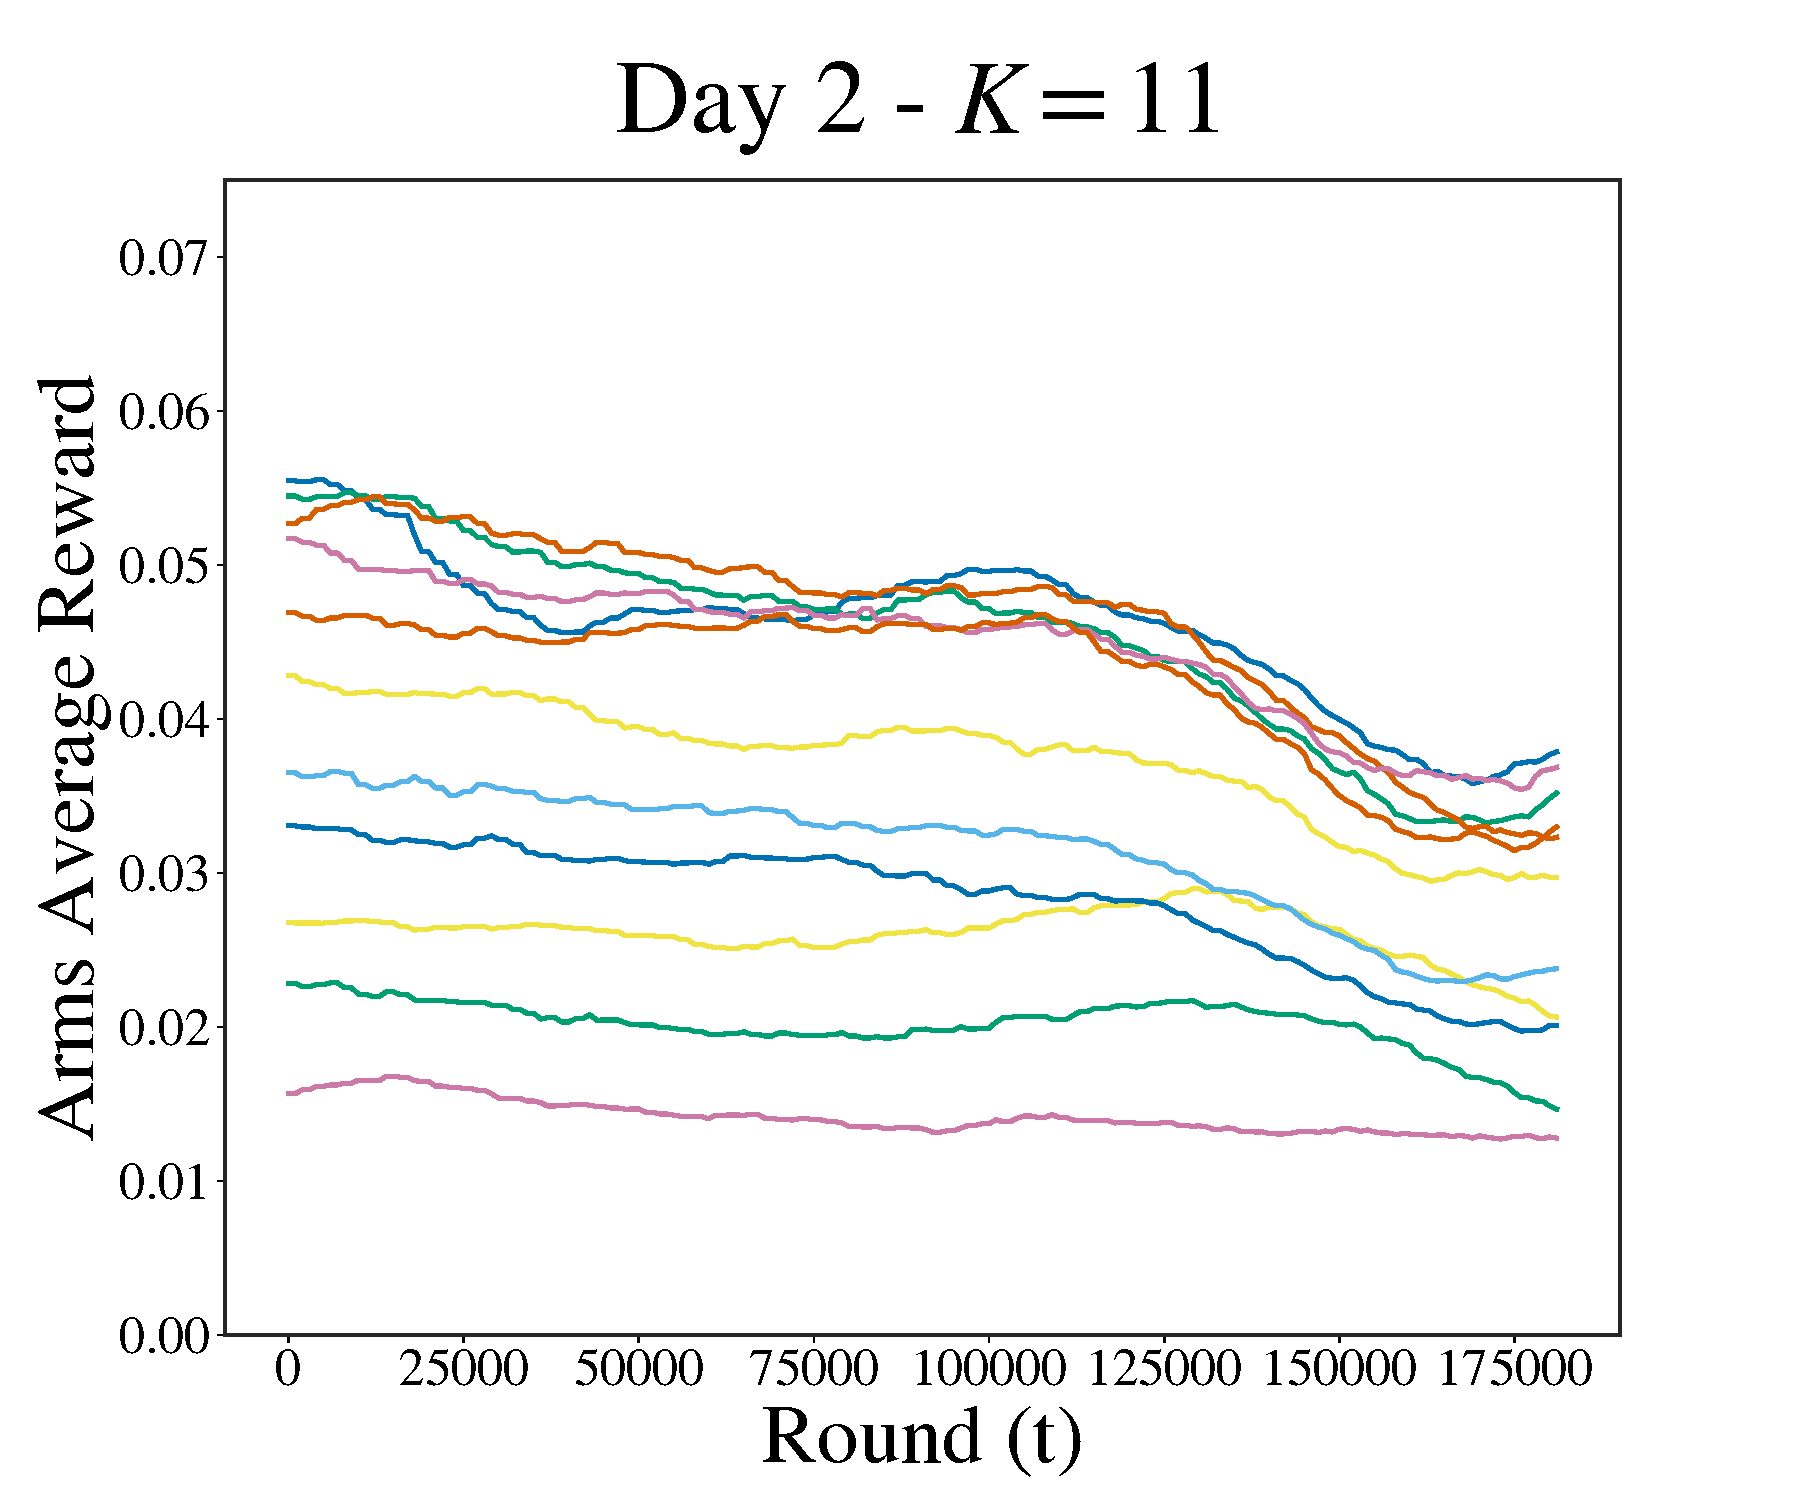
\includegraphics[clip, width= 0.495\textwidth]{4Restless/fig/reward_plot_day2.pdf}
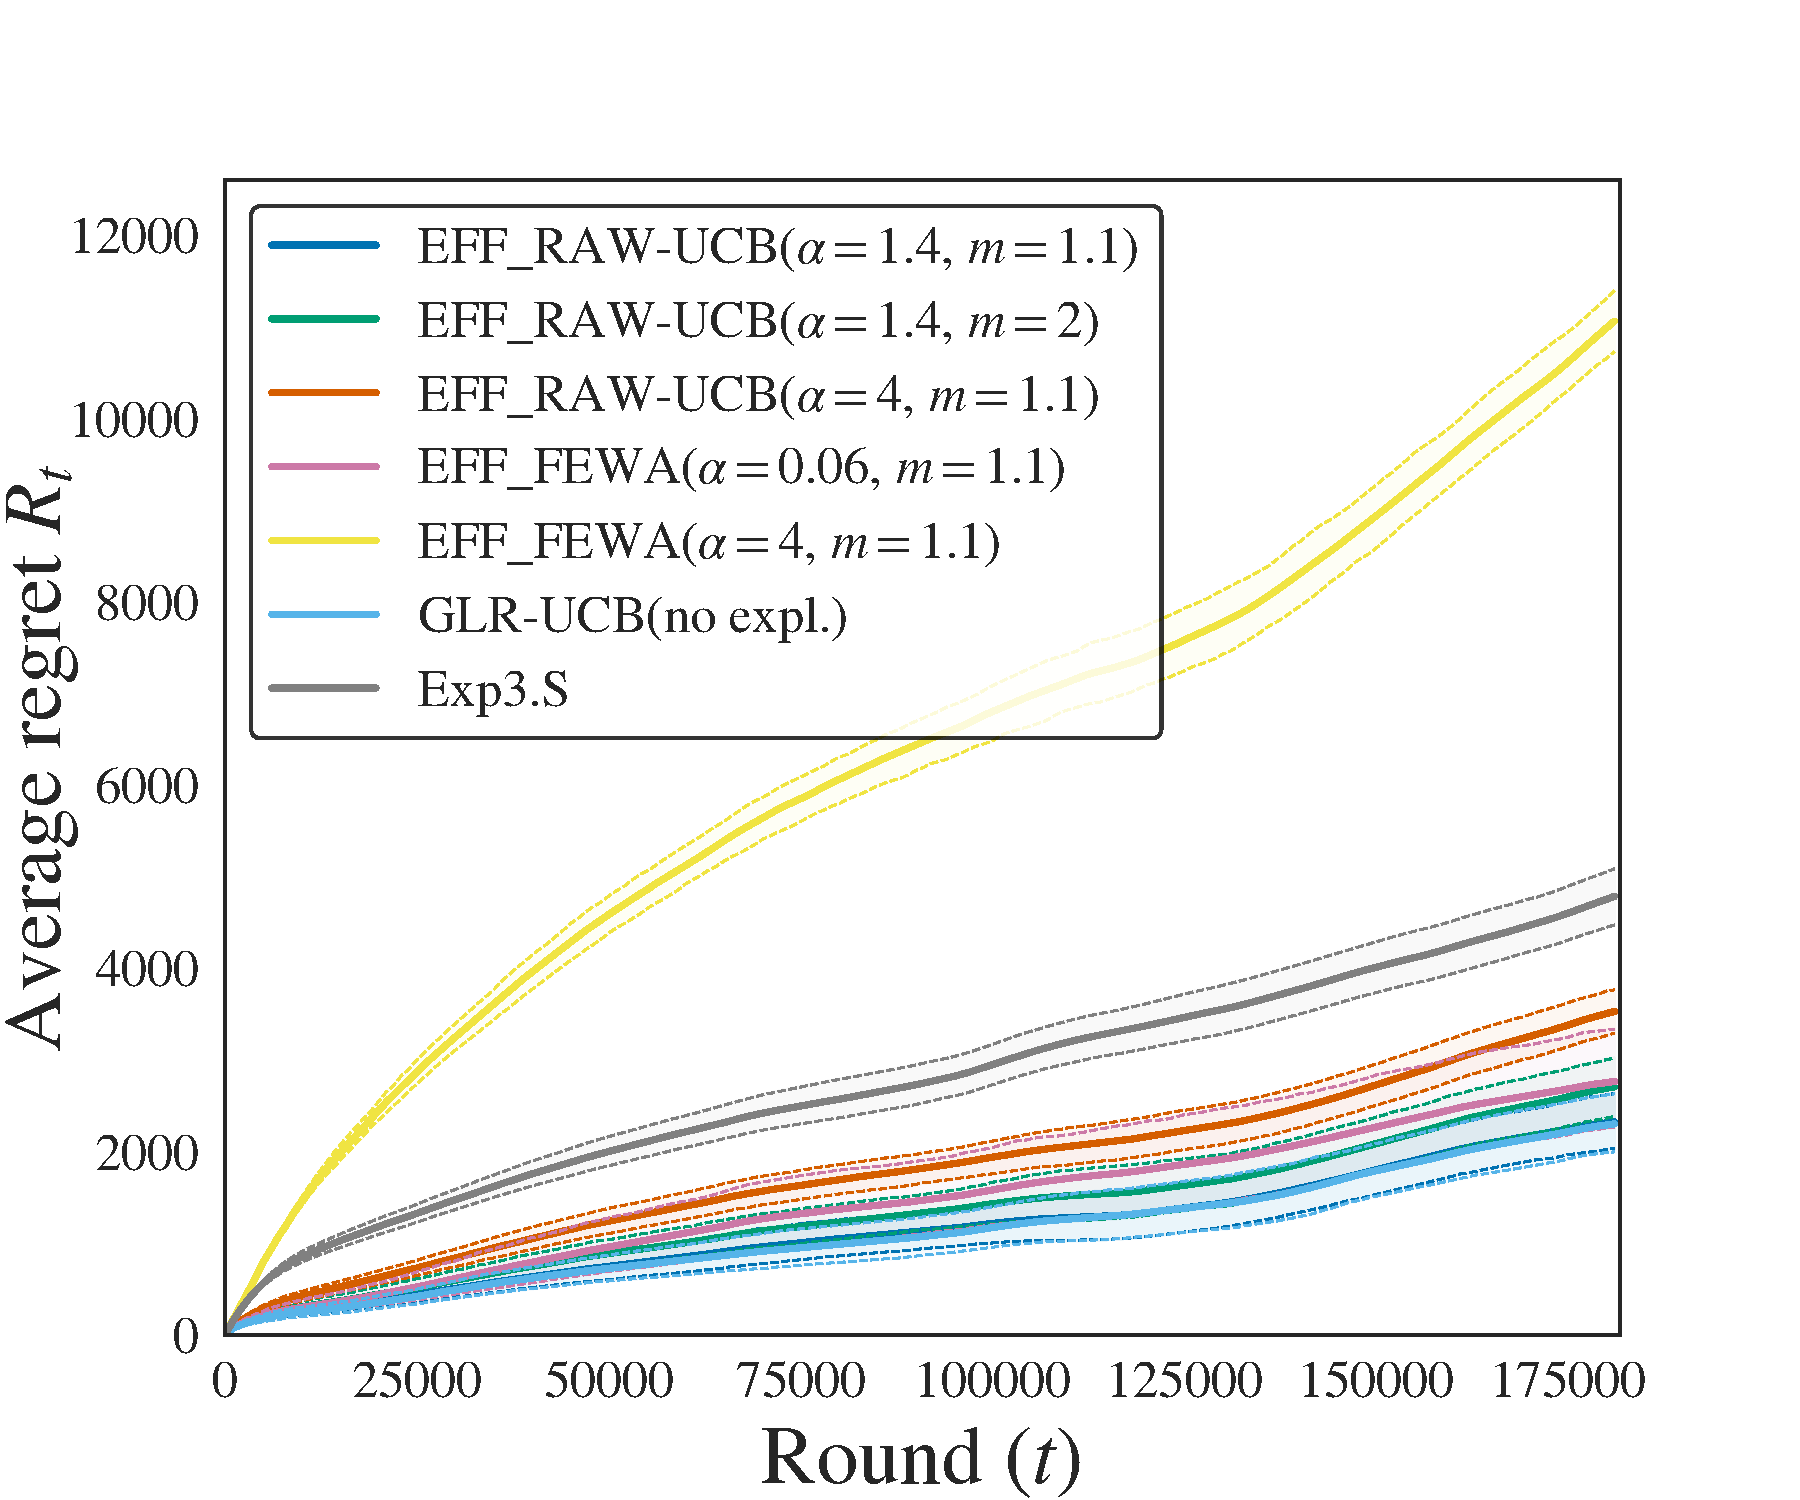
\includegraphics[clip, width= 0.495\textwidth]{4Restless/fig/DAY2.pdf}
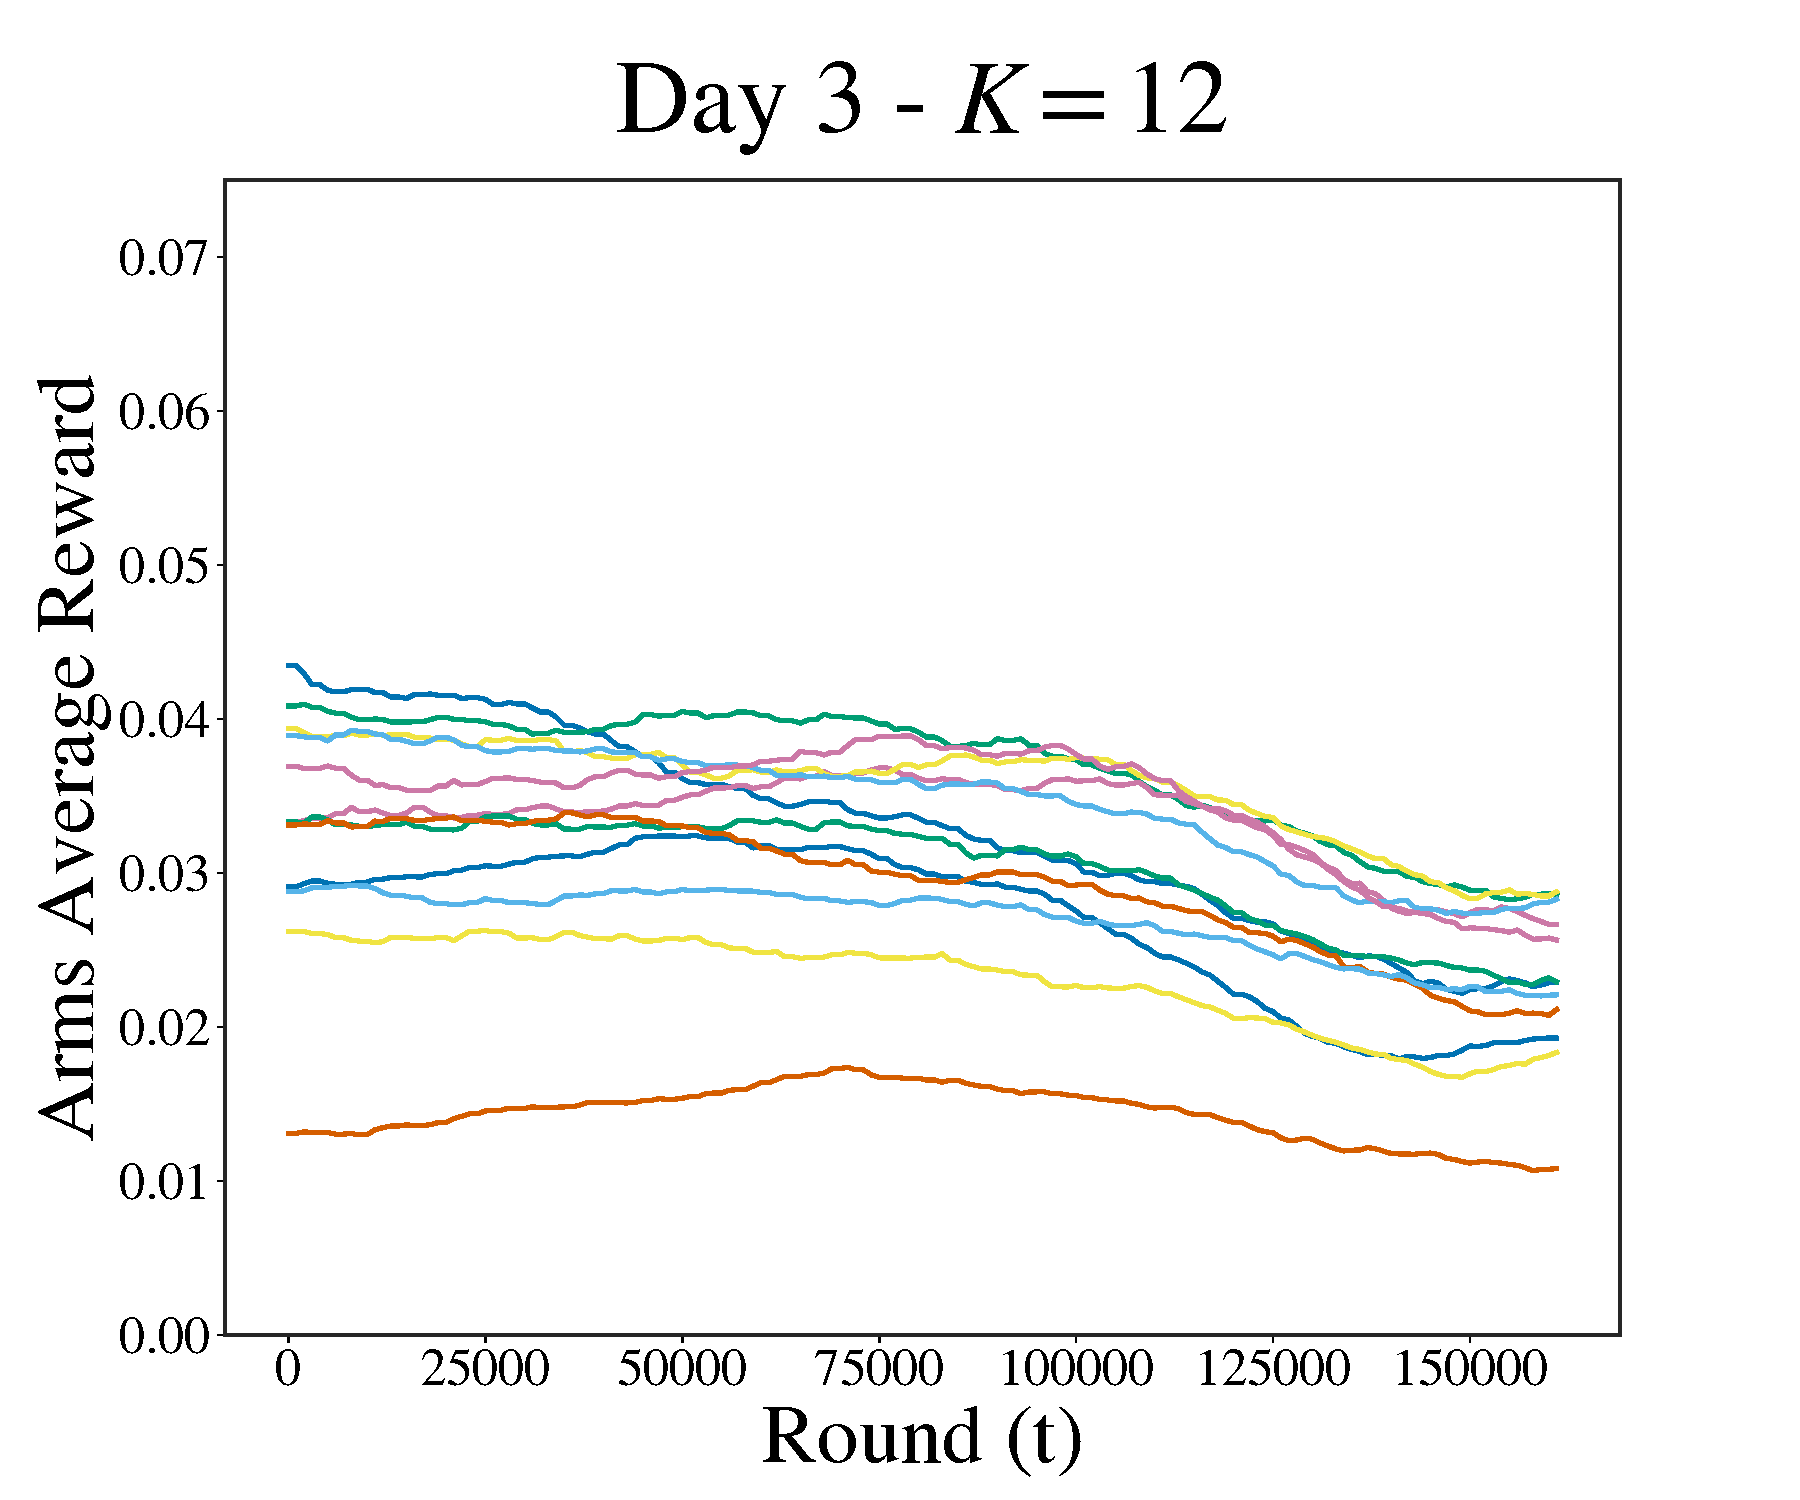
\includegraphics[clip, width= 0.495\textwidth]{4Restless/fig/reward_plot_day3.pdf}
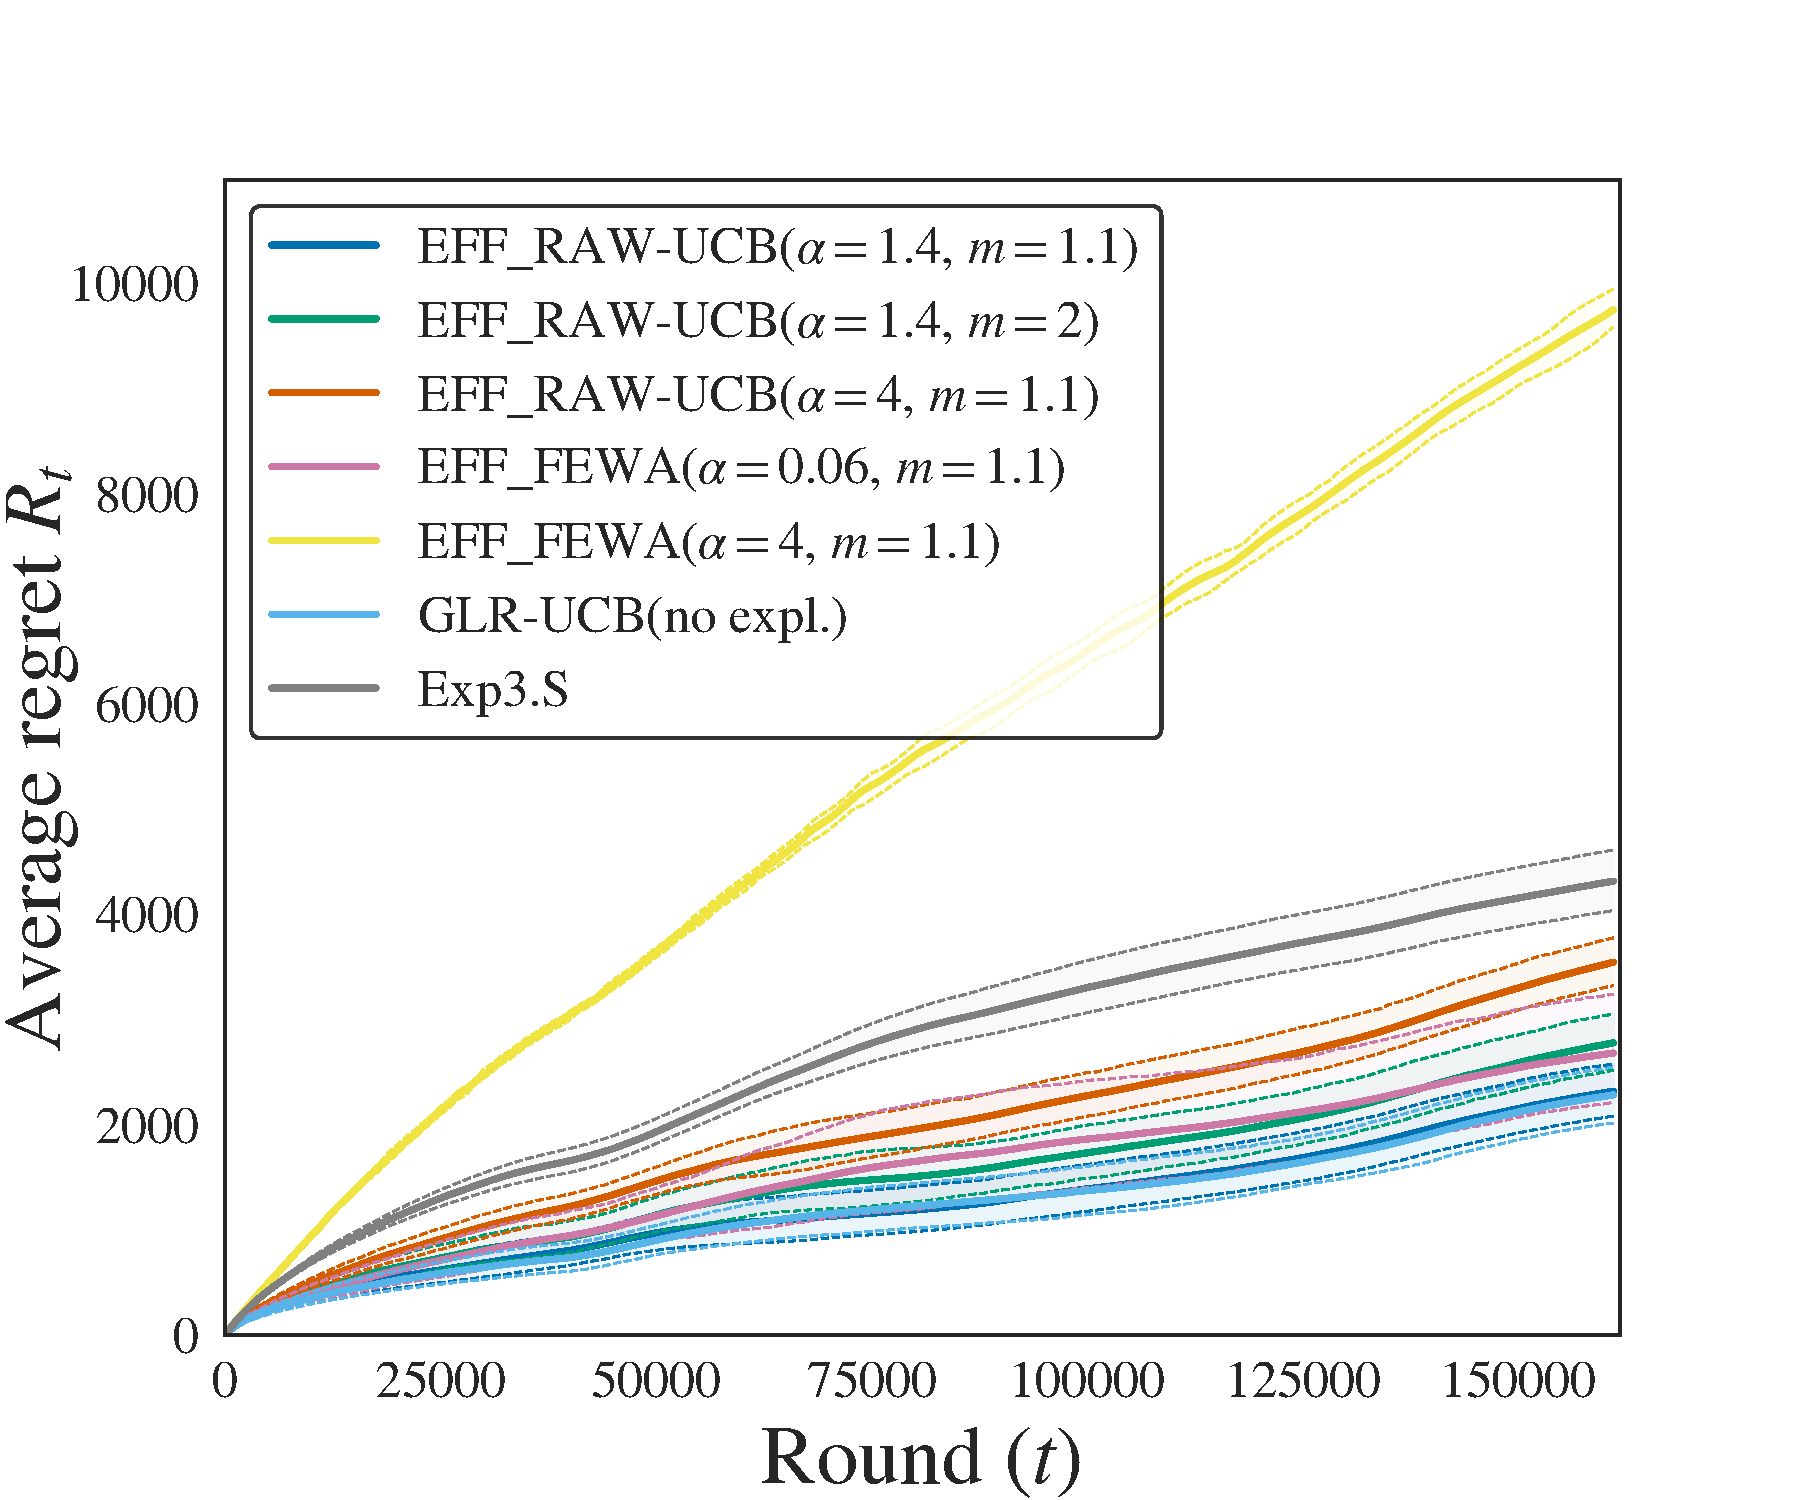
\includegraphics[clip, width= 0.495\textwidth]{4Restless/fig/DAY3.pdf}
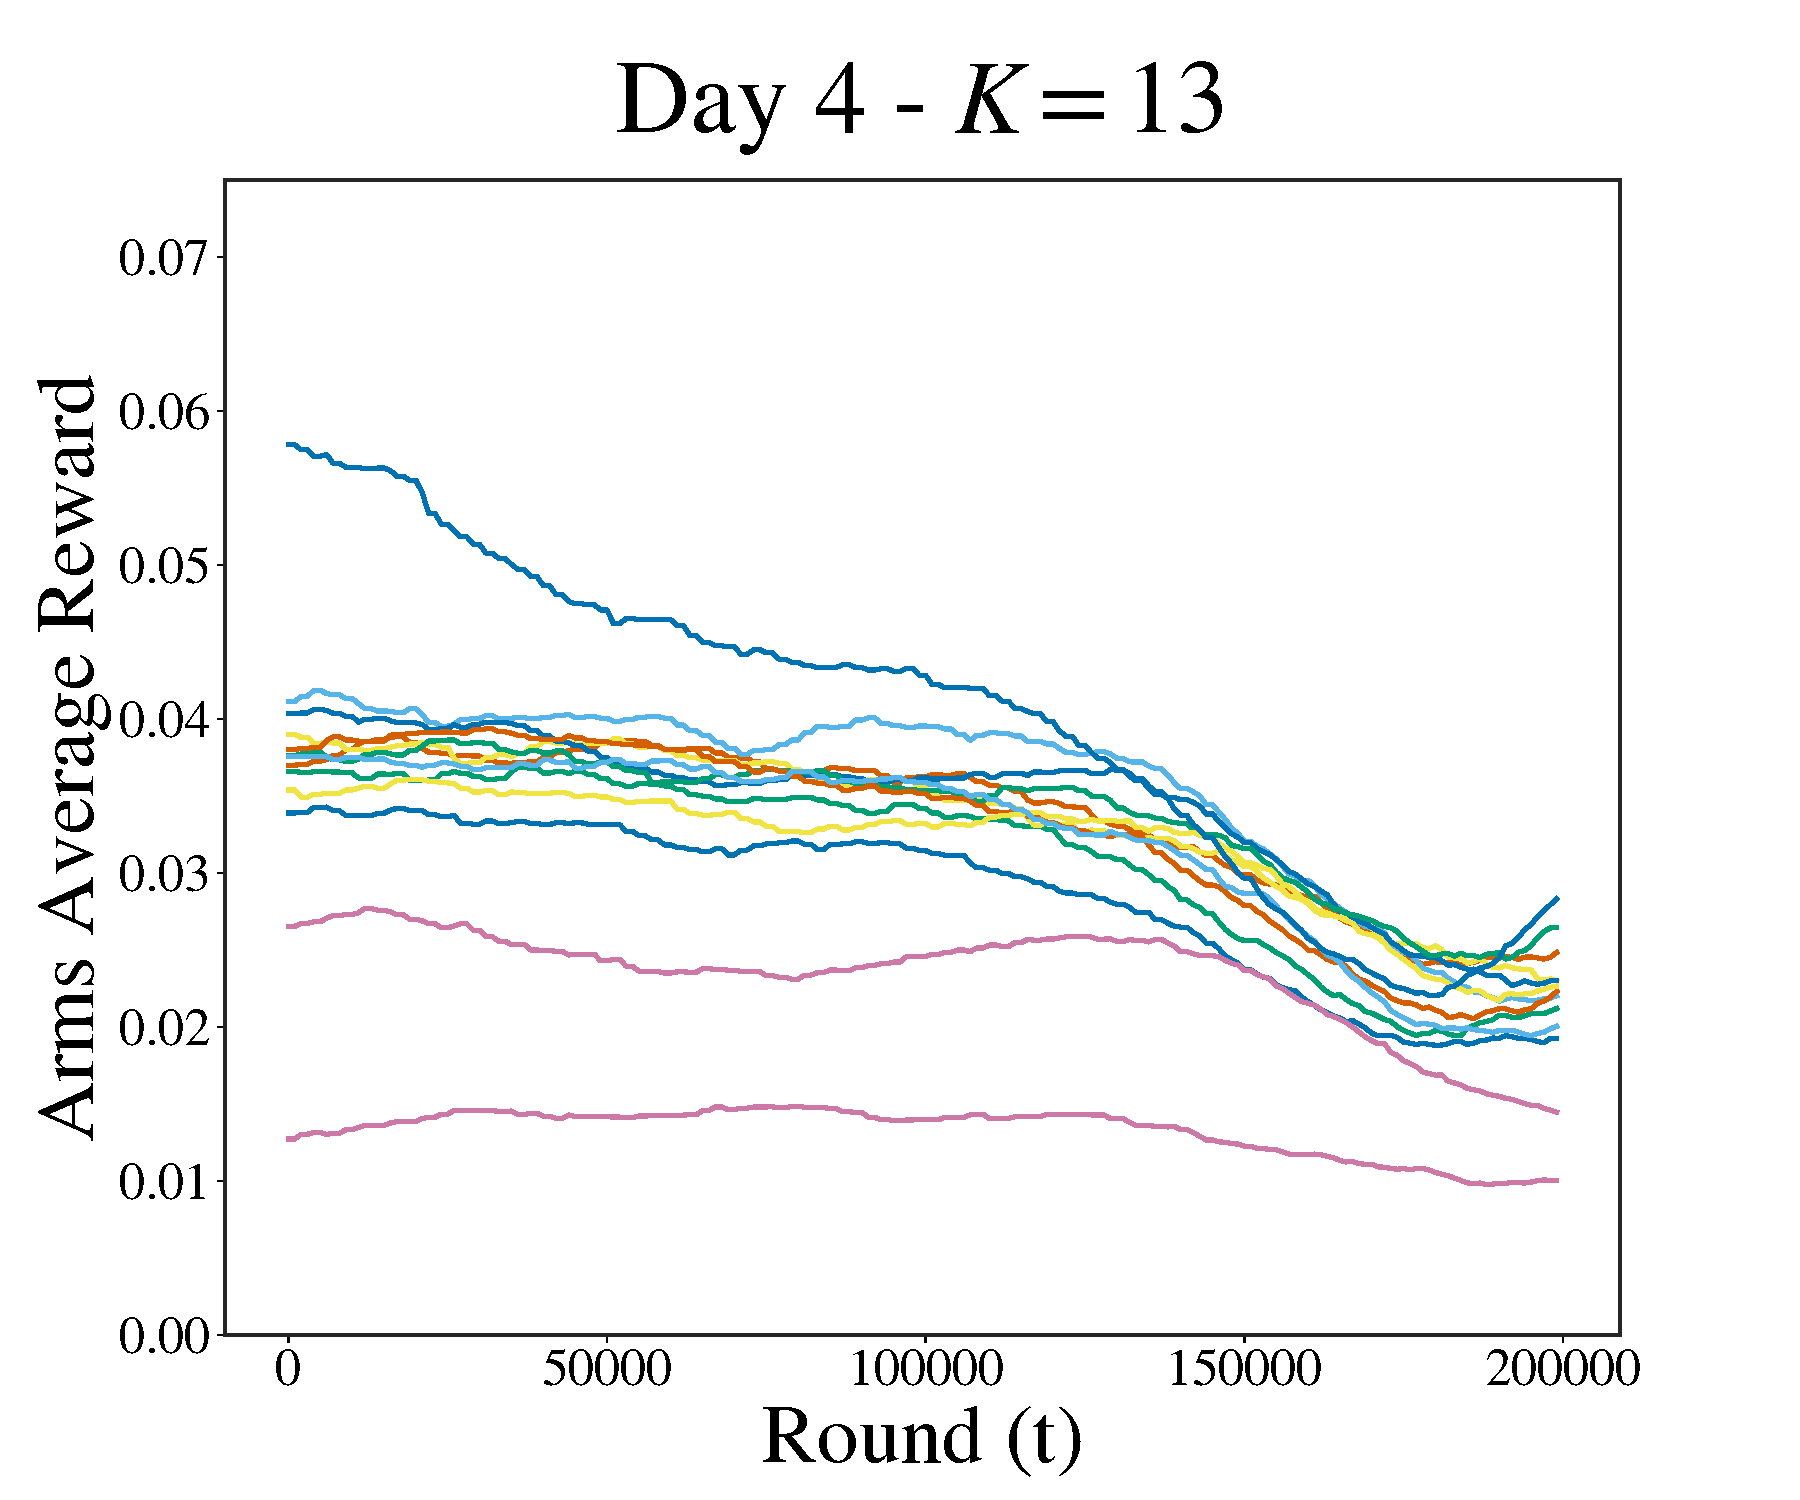
\includegraphics[clip, width= 0.495\textwidth]{4Restless/fig/reward_plot_day4.pdf}
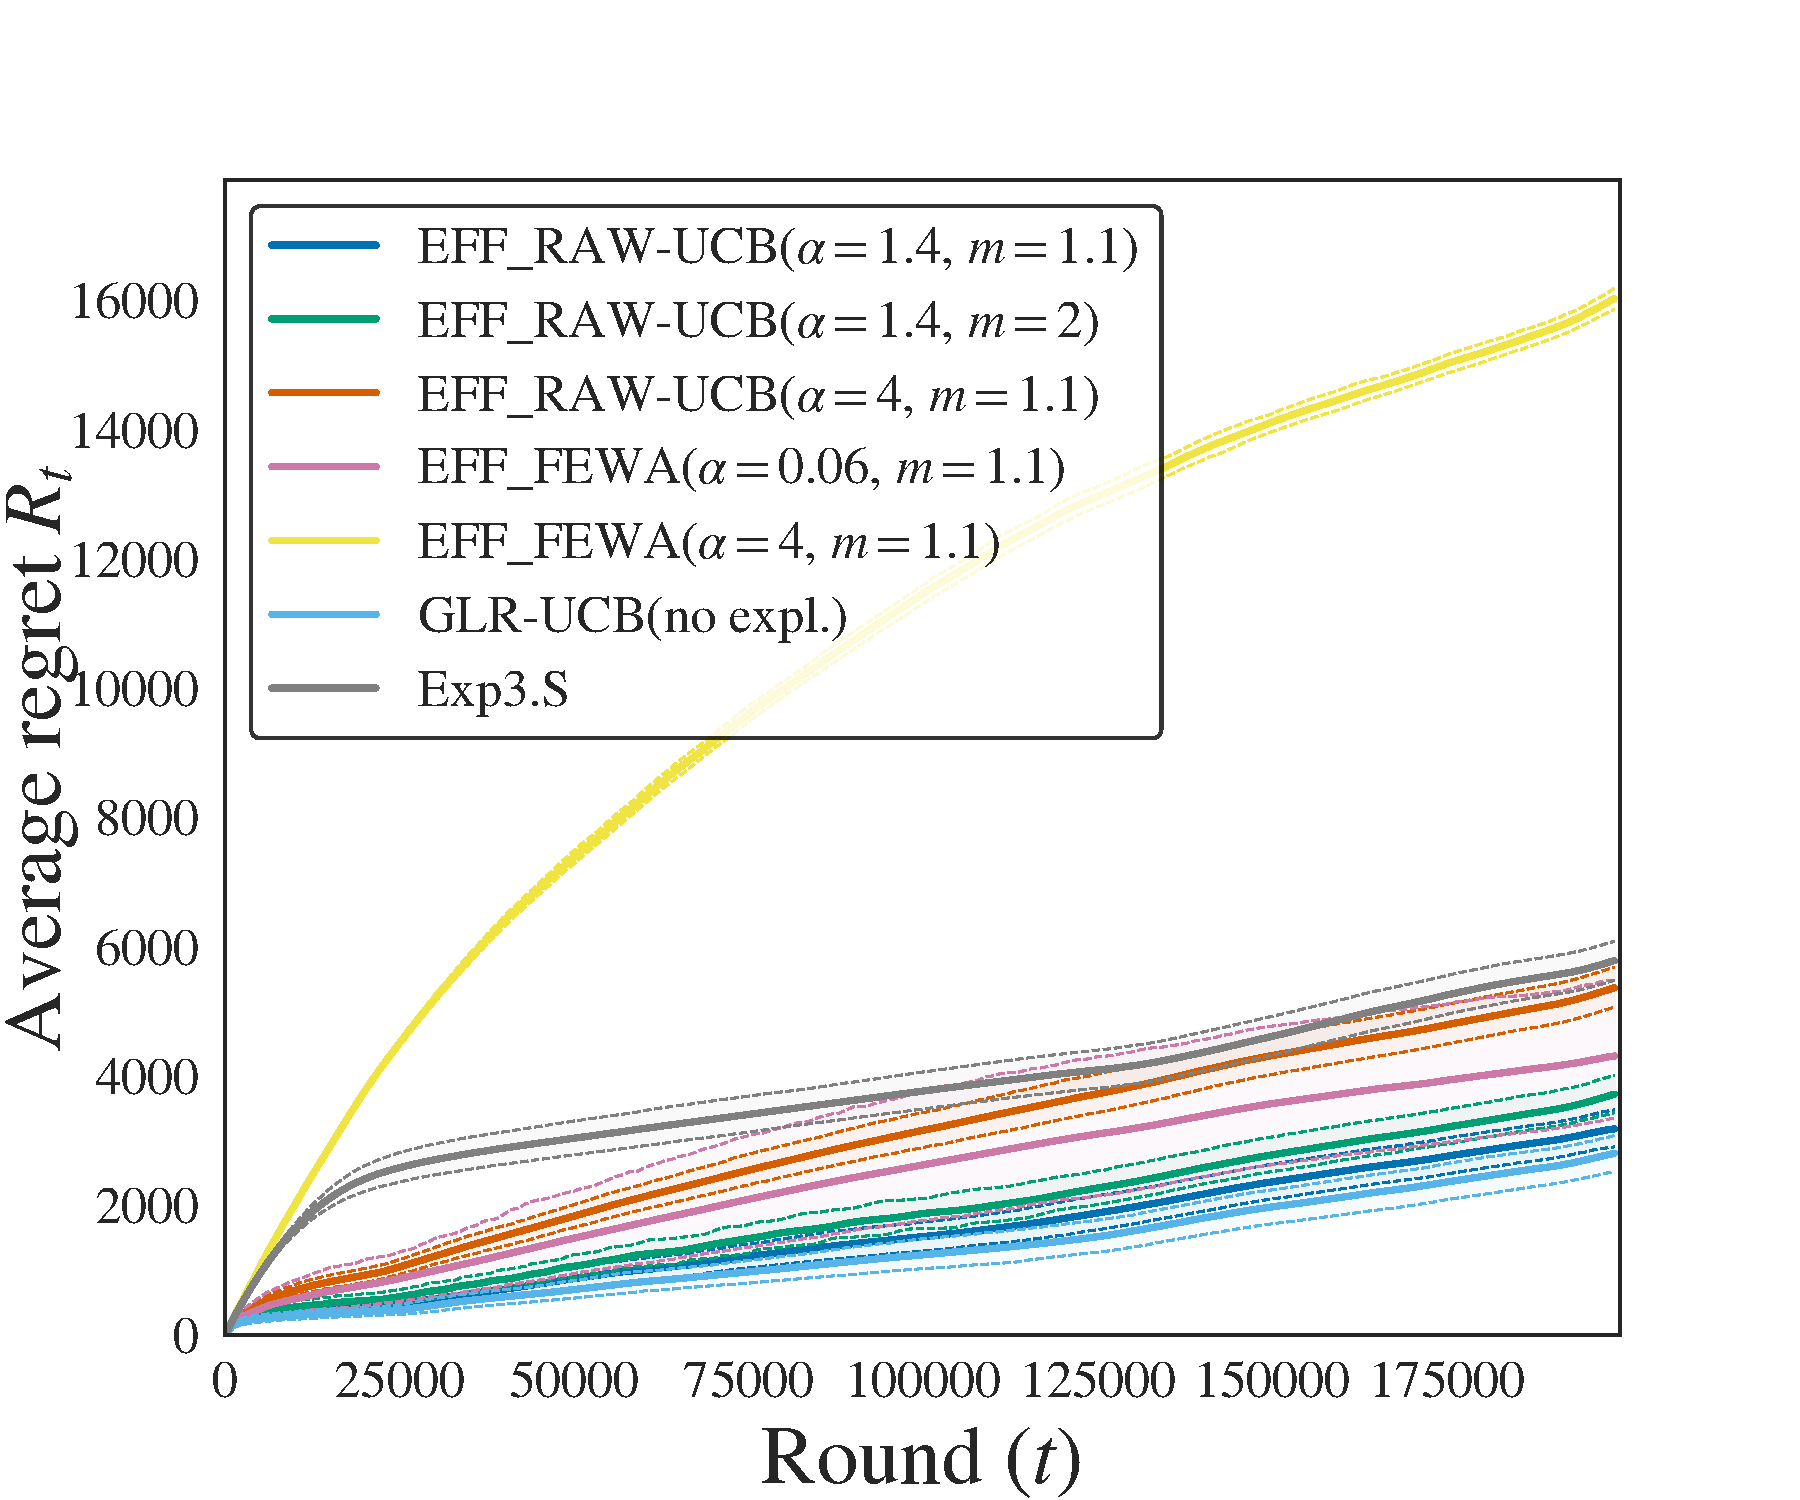
\includegraphics[clip, width= 0.495\textwidth]{4Restless/fig/DAY4.pdf}
\end{figure*}

\begin{figure*}[p!]
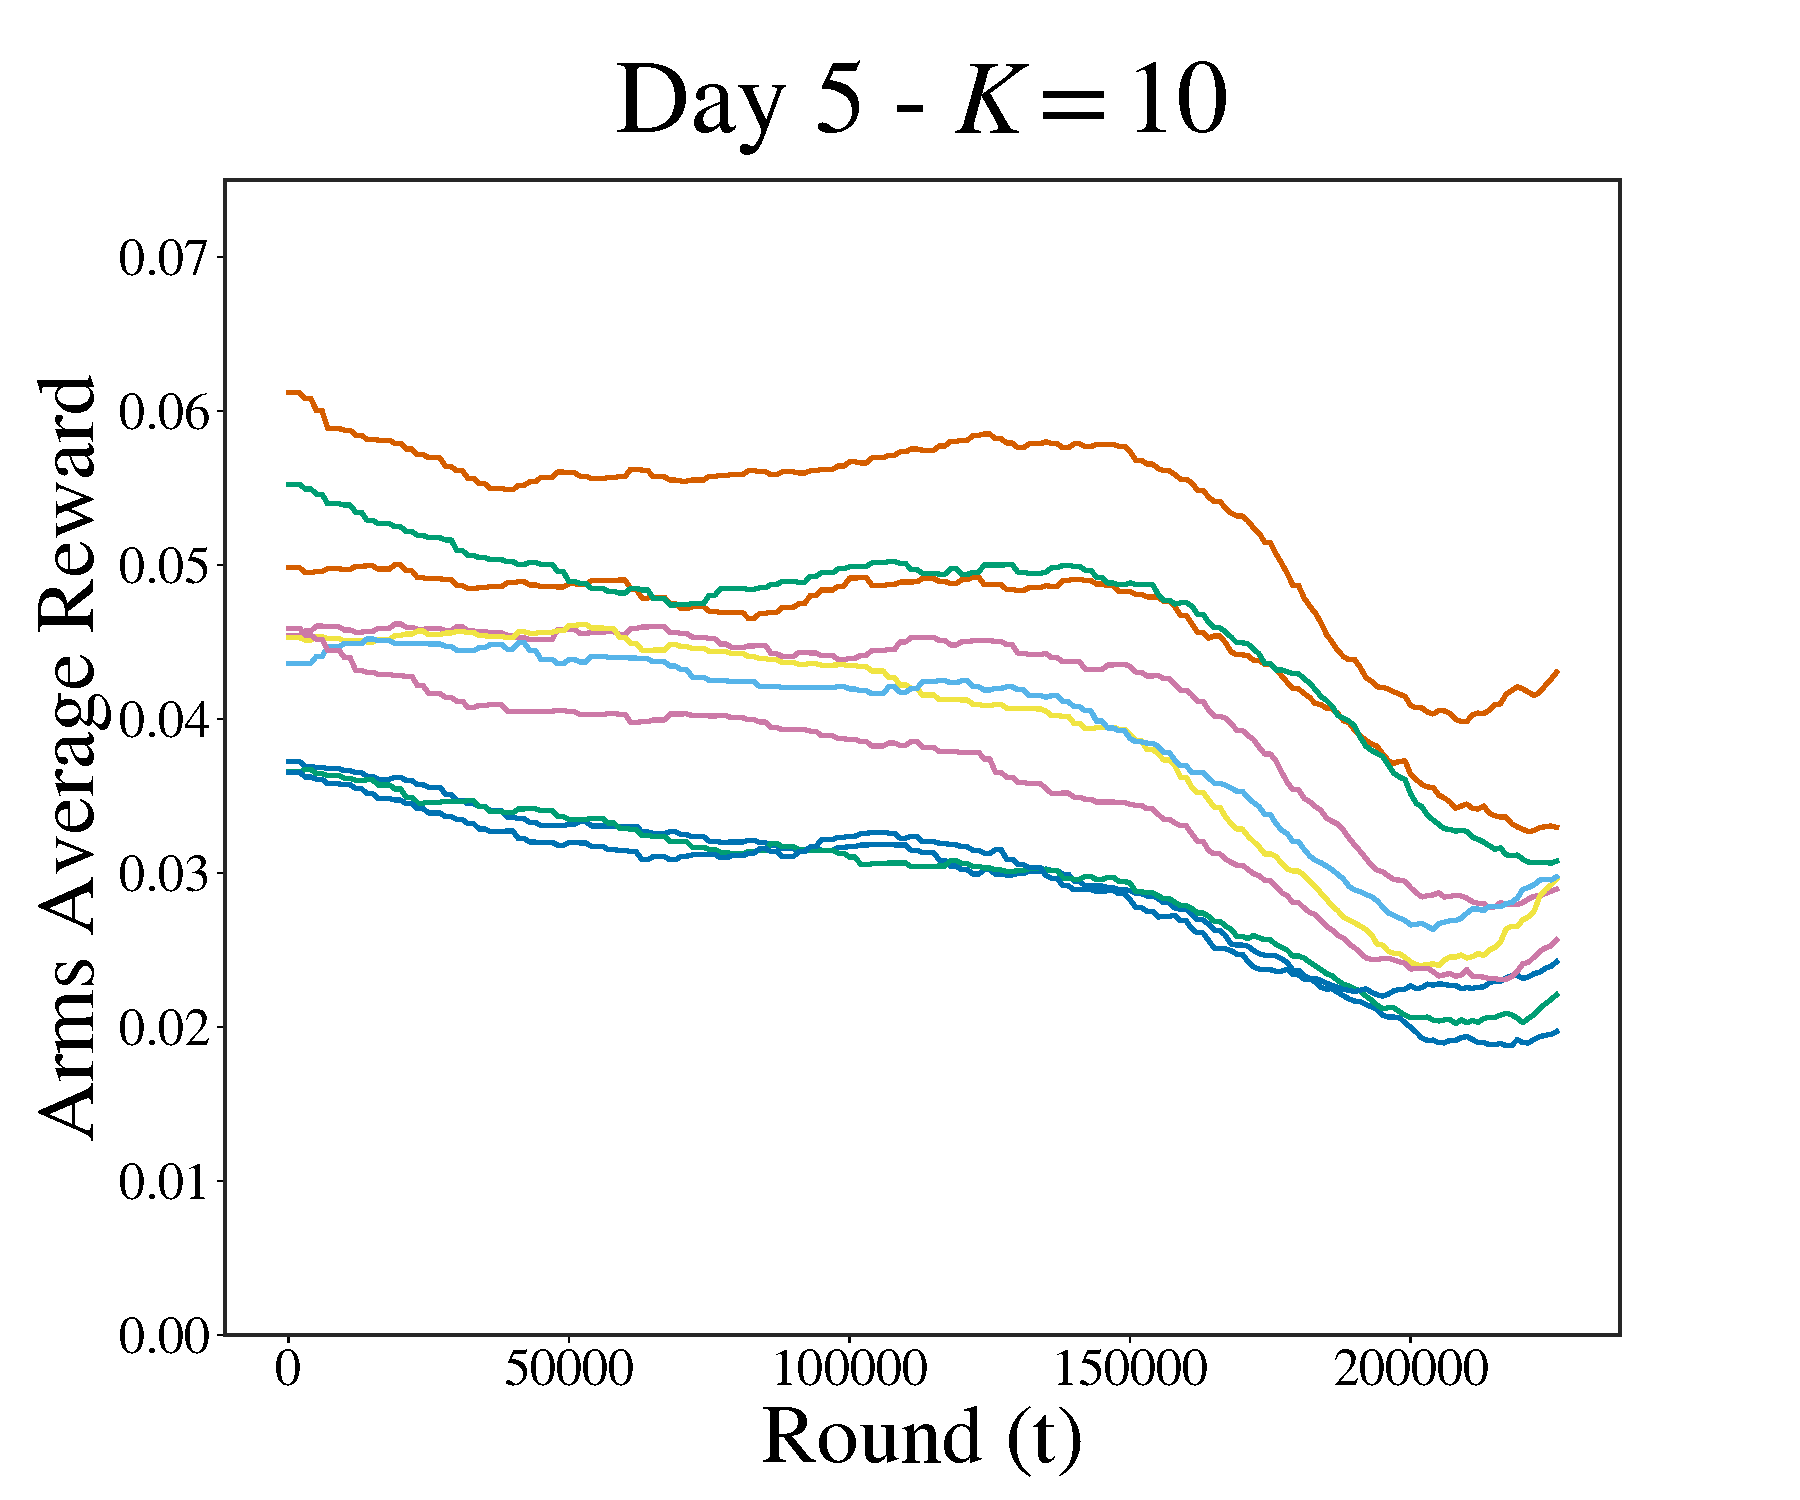
\includegraphics[clip, width= 0.495\textwidth]{4Restless/fig/reward_plot_day5.pdf}
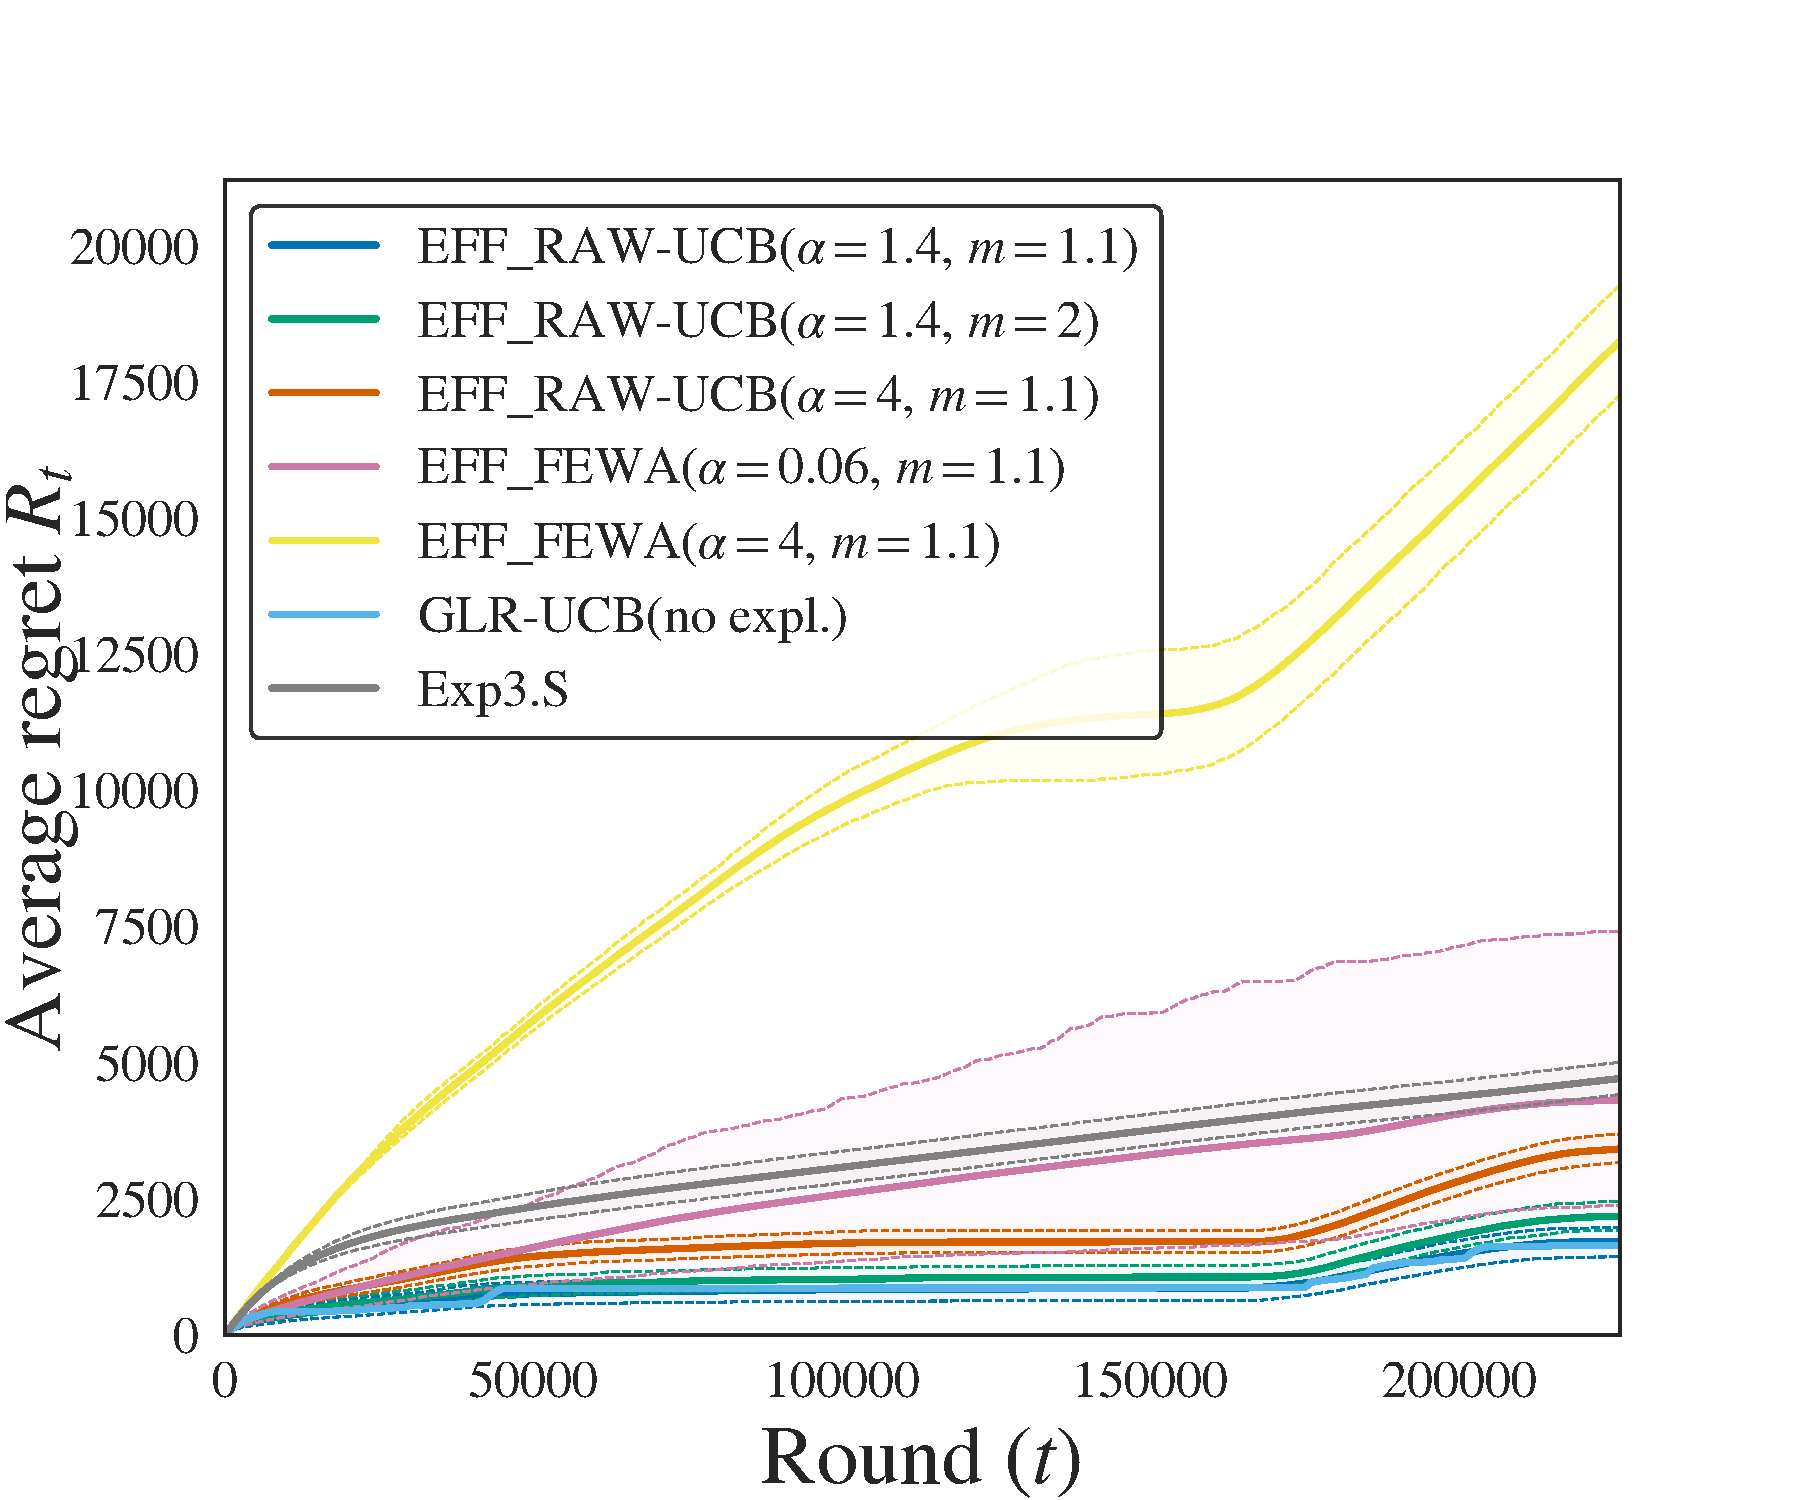
\includegraphics[clip, width= 0.495\textwidth]{4Restless/fig/DAY5.pdf}
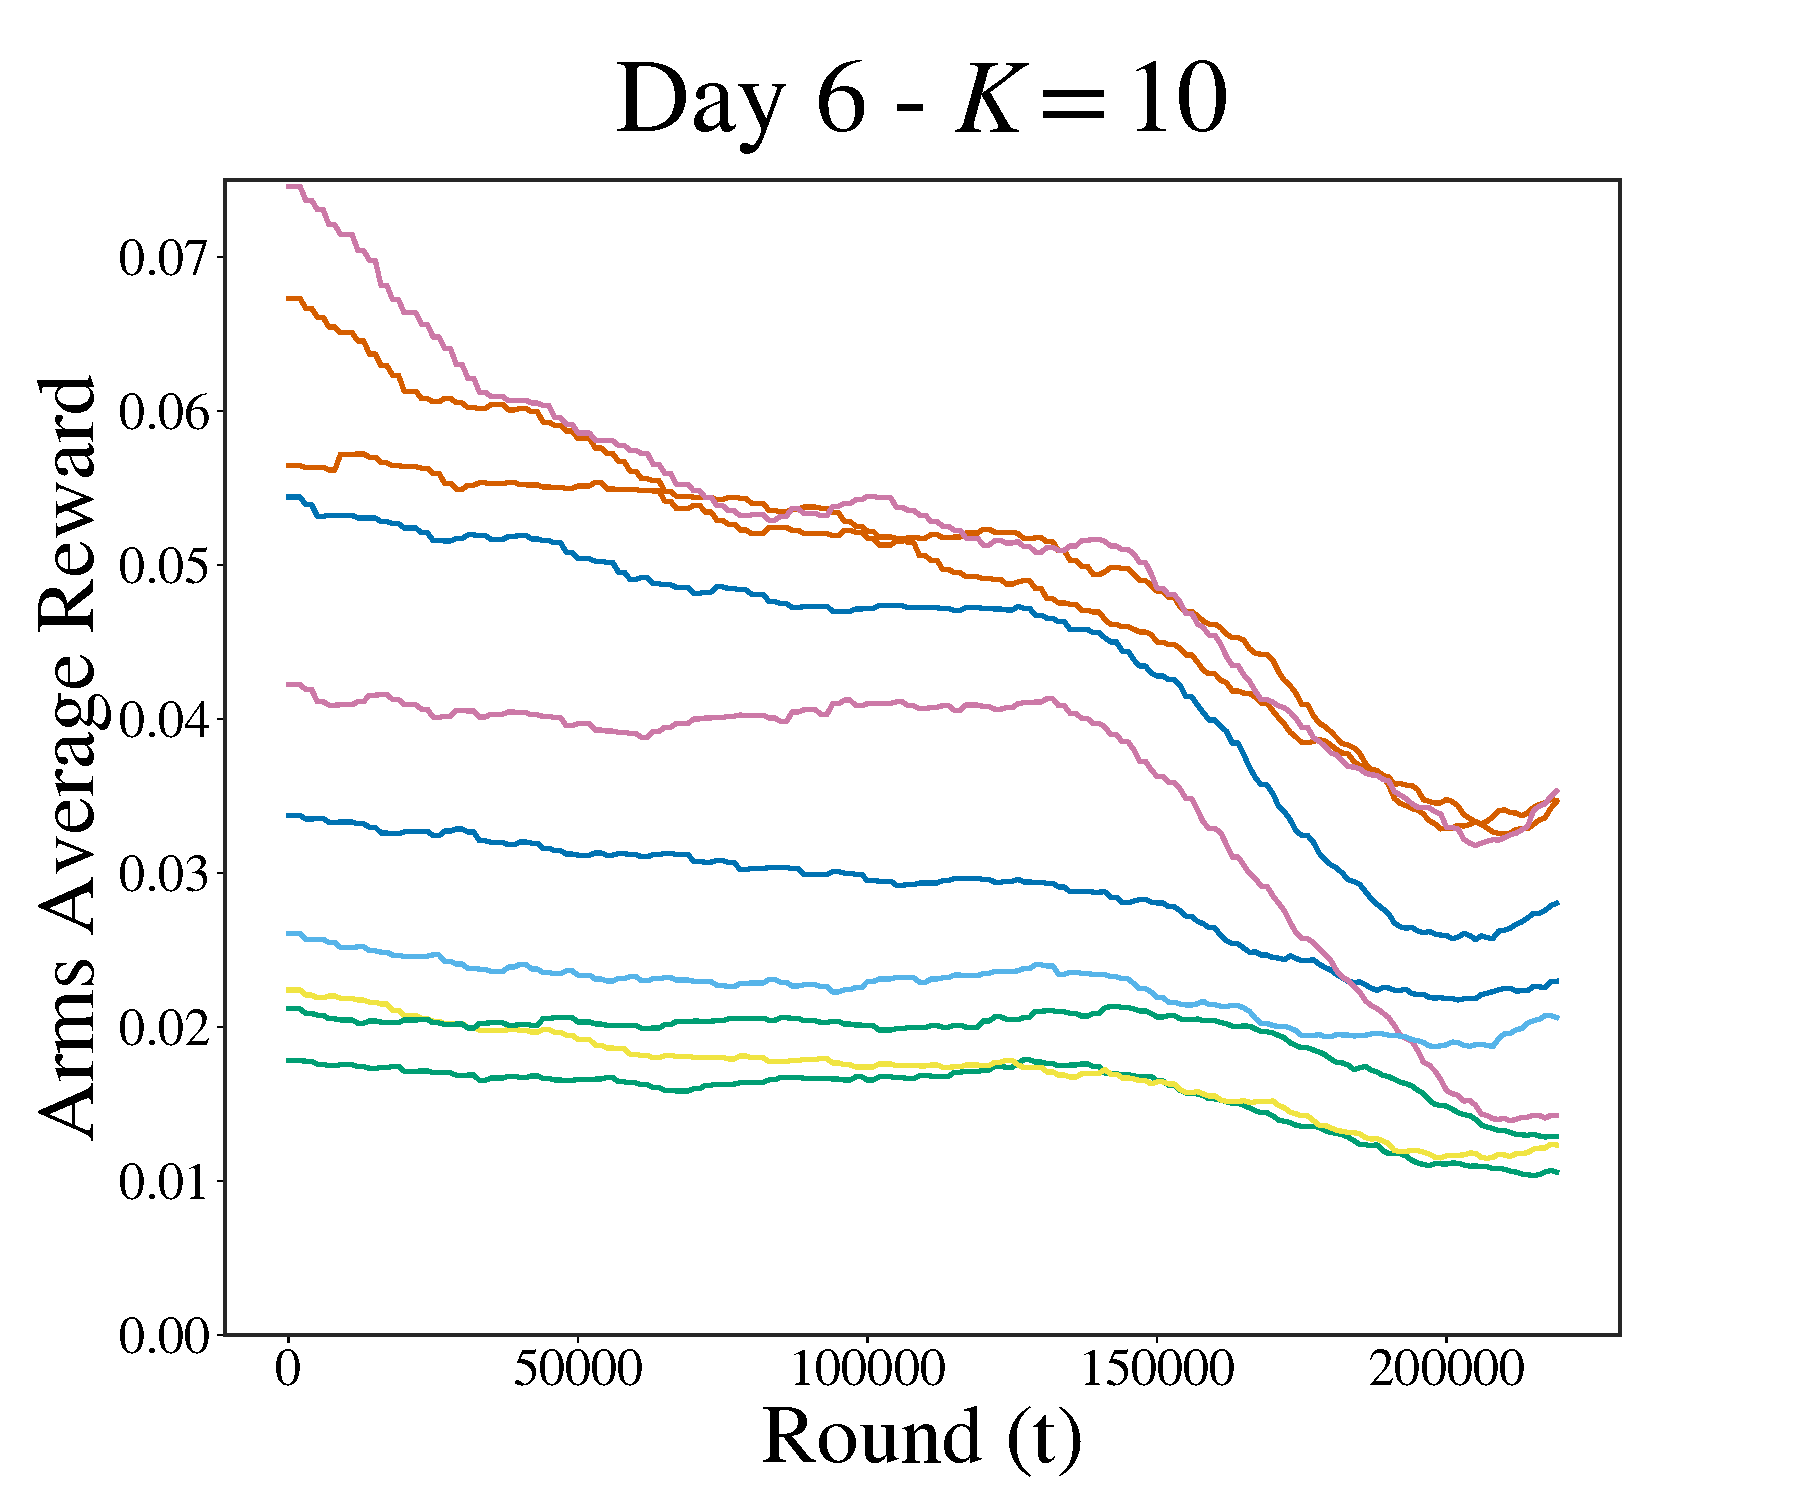
\includegraphics[clip, width= 0.495\textwidth]{4Restless/fig/reward_plot_day6.pdf}
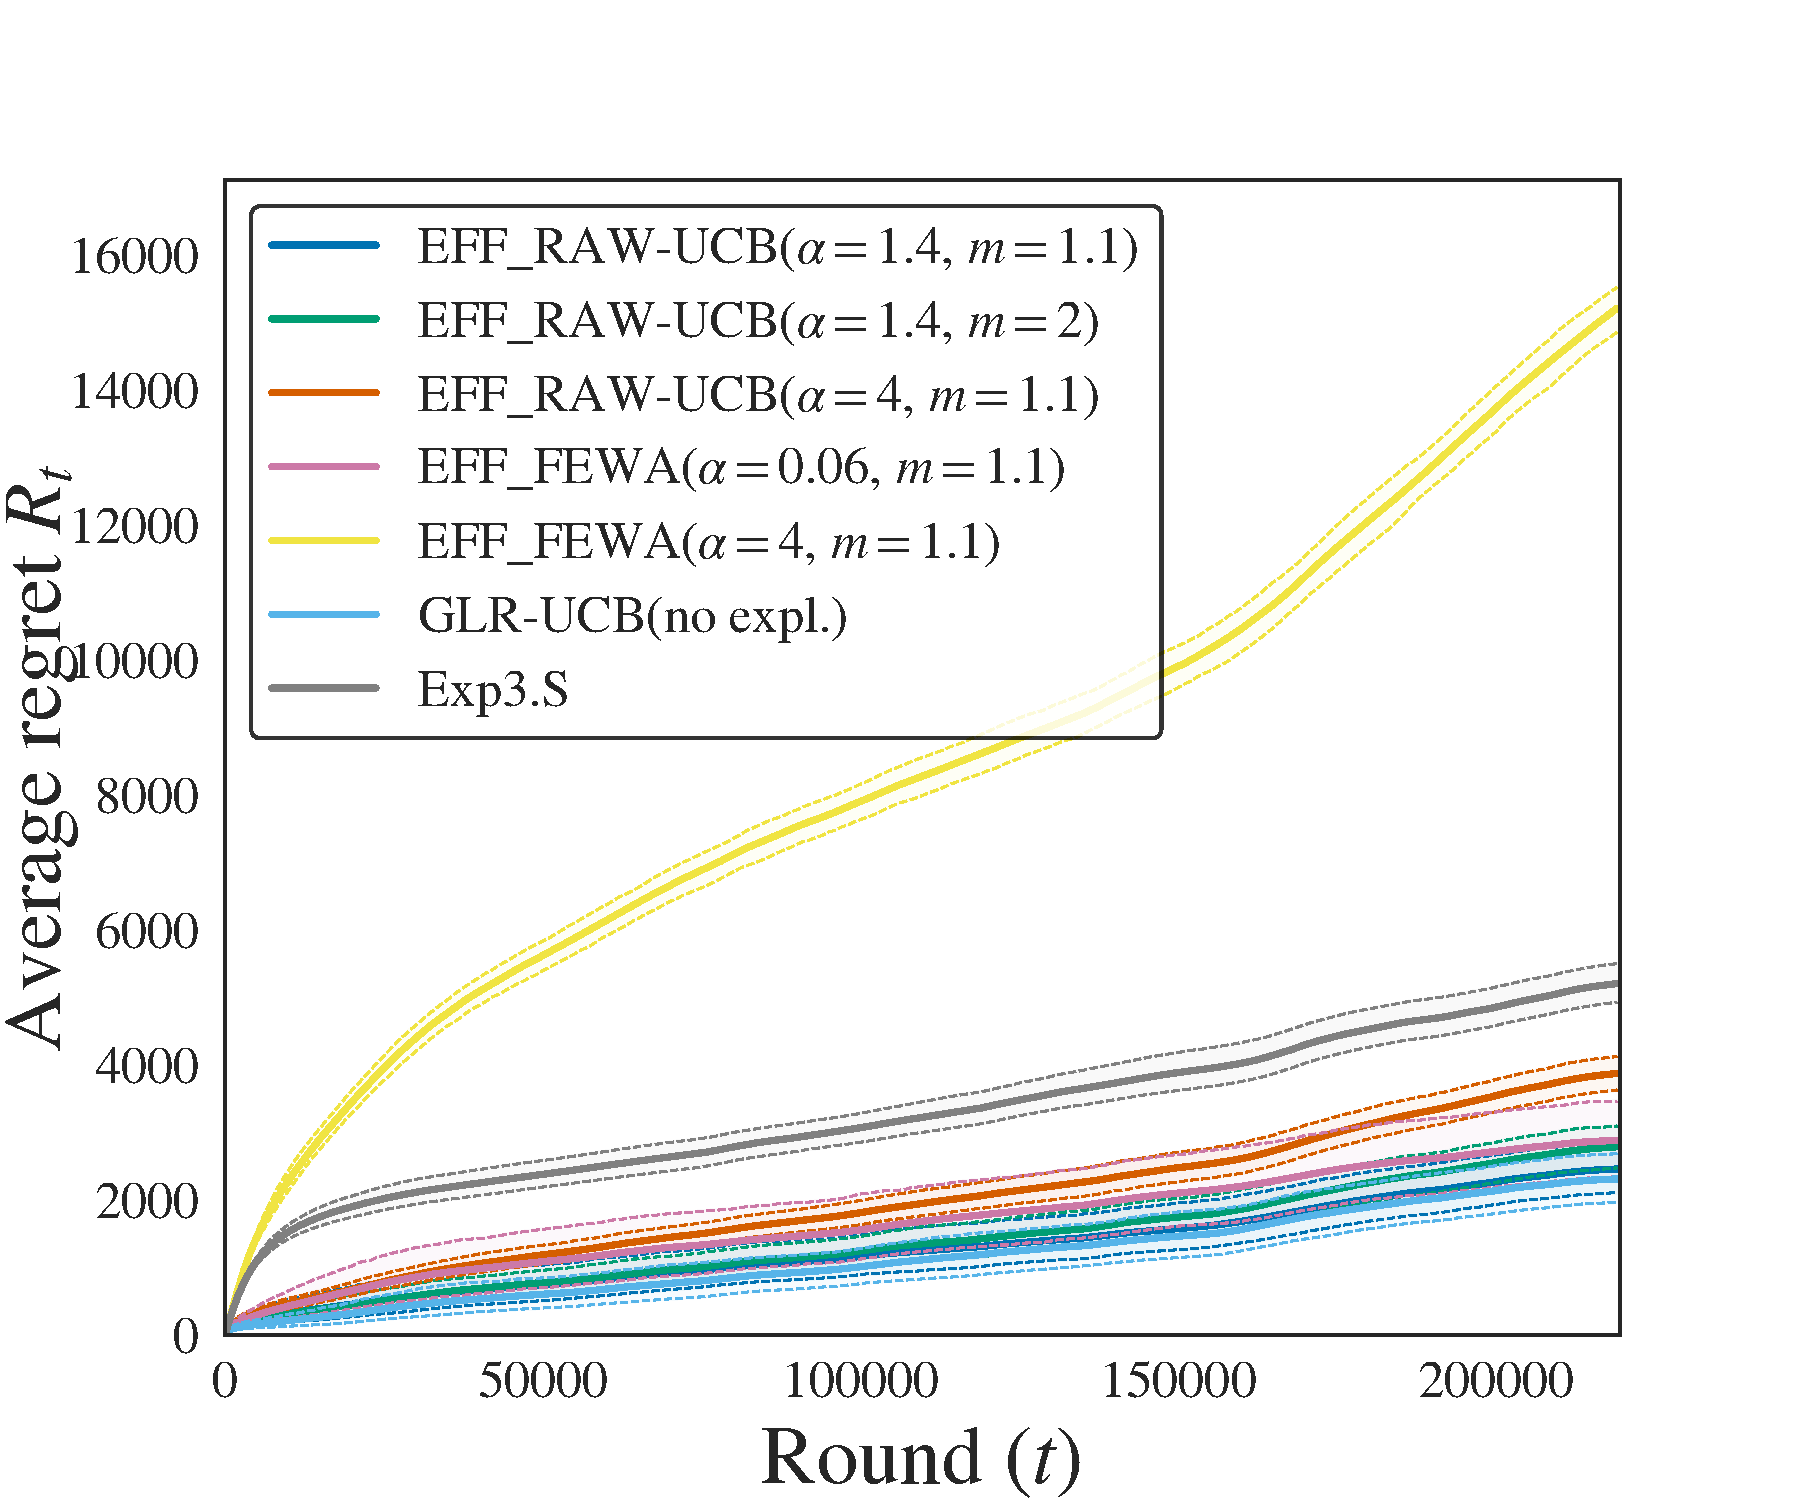
\includegraphics[clip, width= 0.495\textwidth]{4Restless/fig/DAY6.pdf}
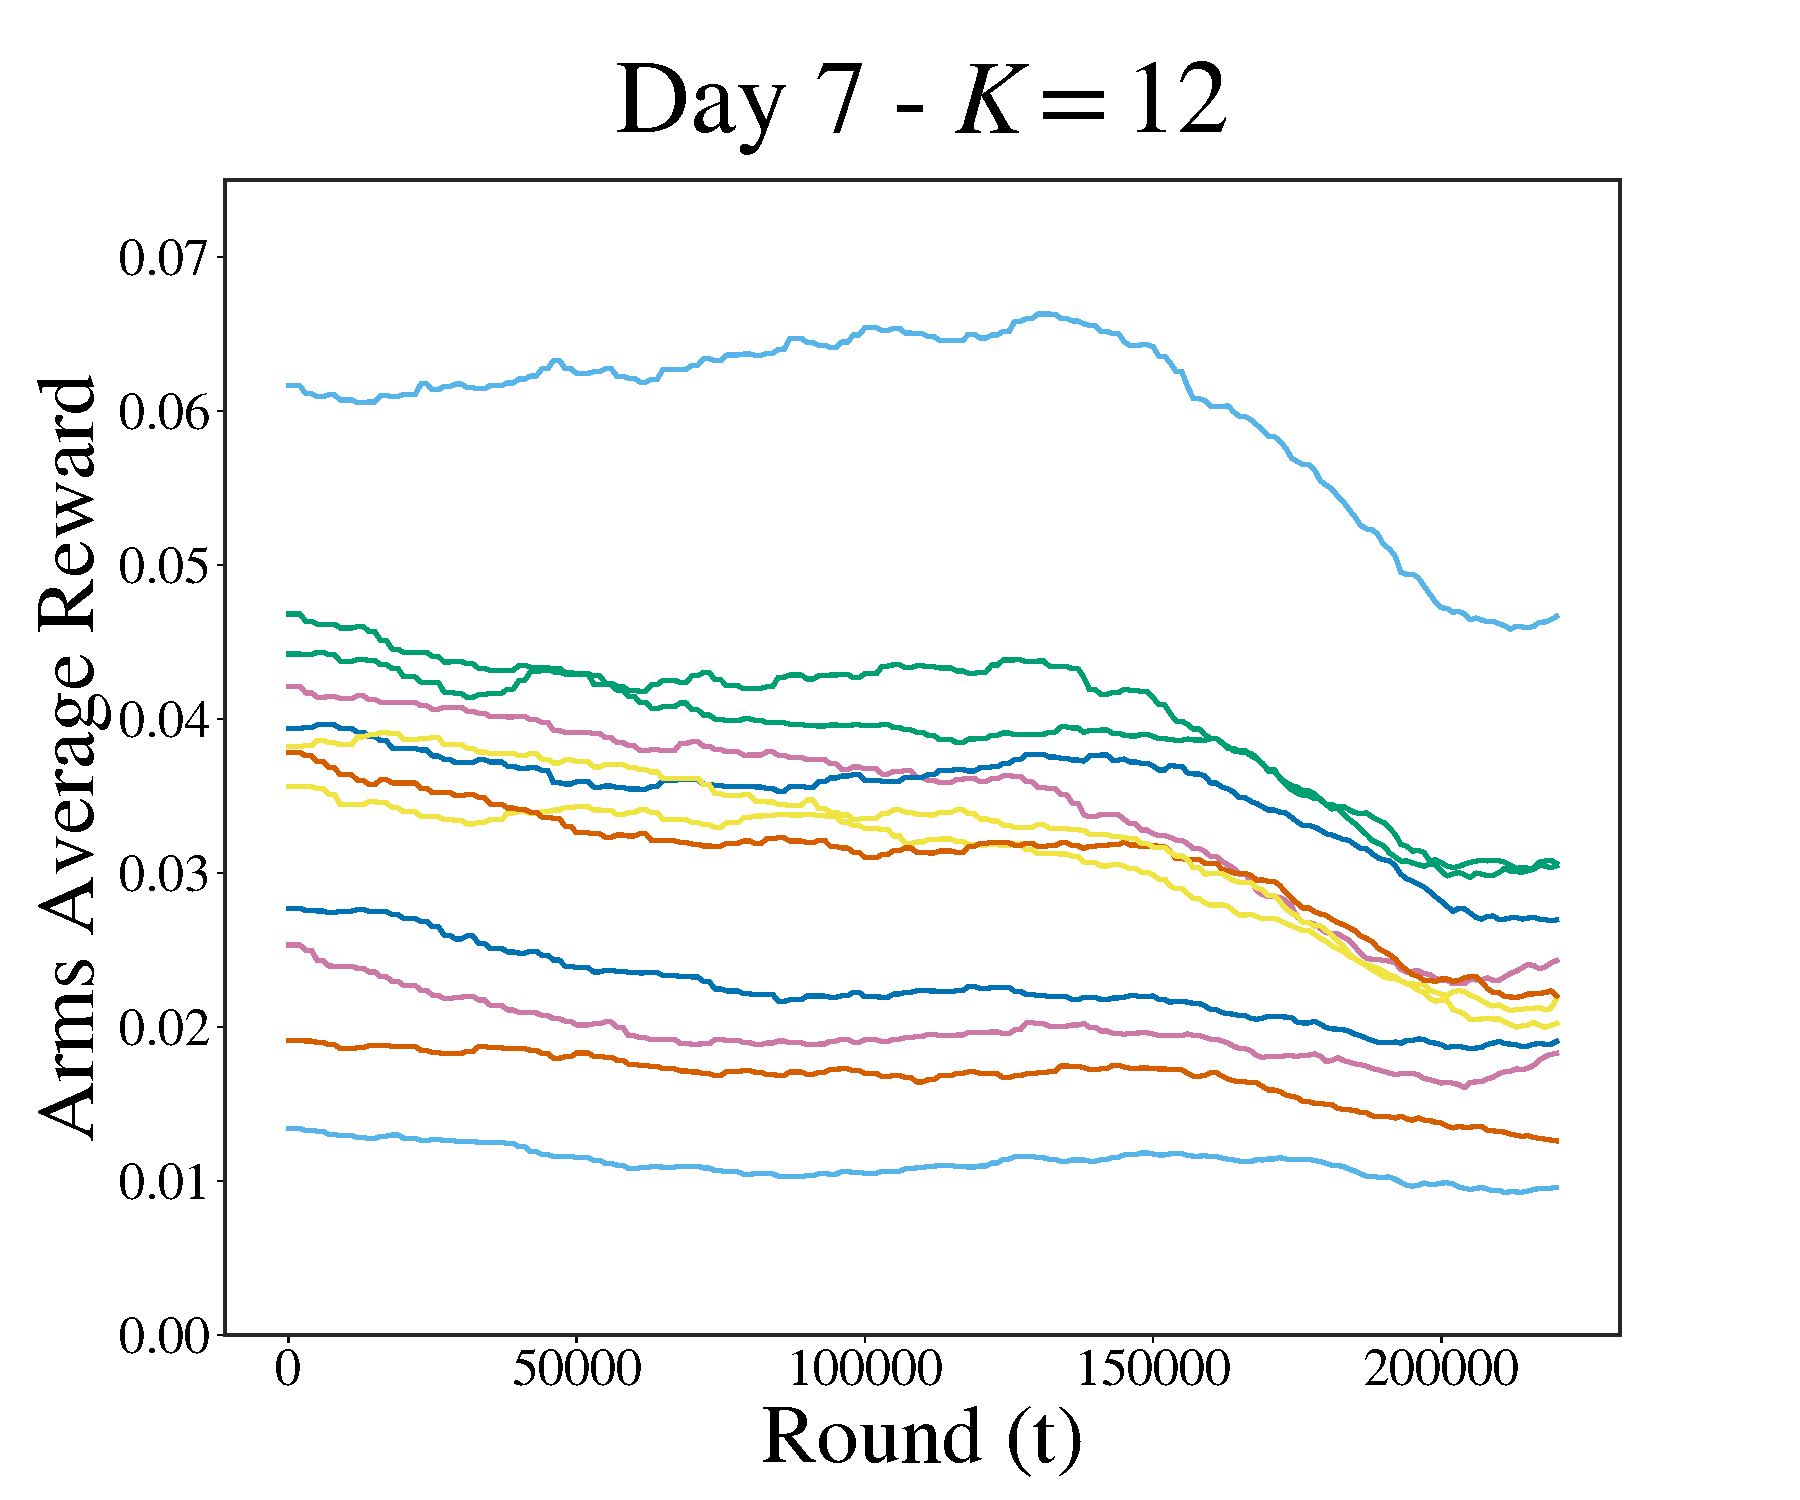
\includegraphics[clip, width= 0.495\textwidth]{4Restless/fig/reward_plot_day7.pdf}
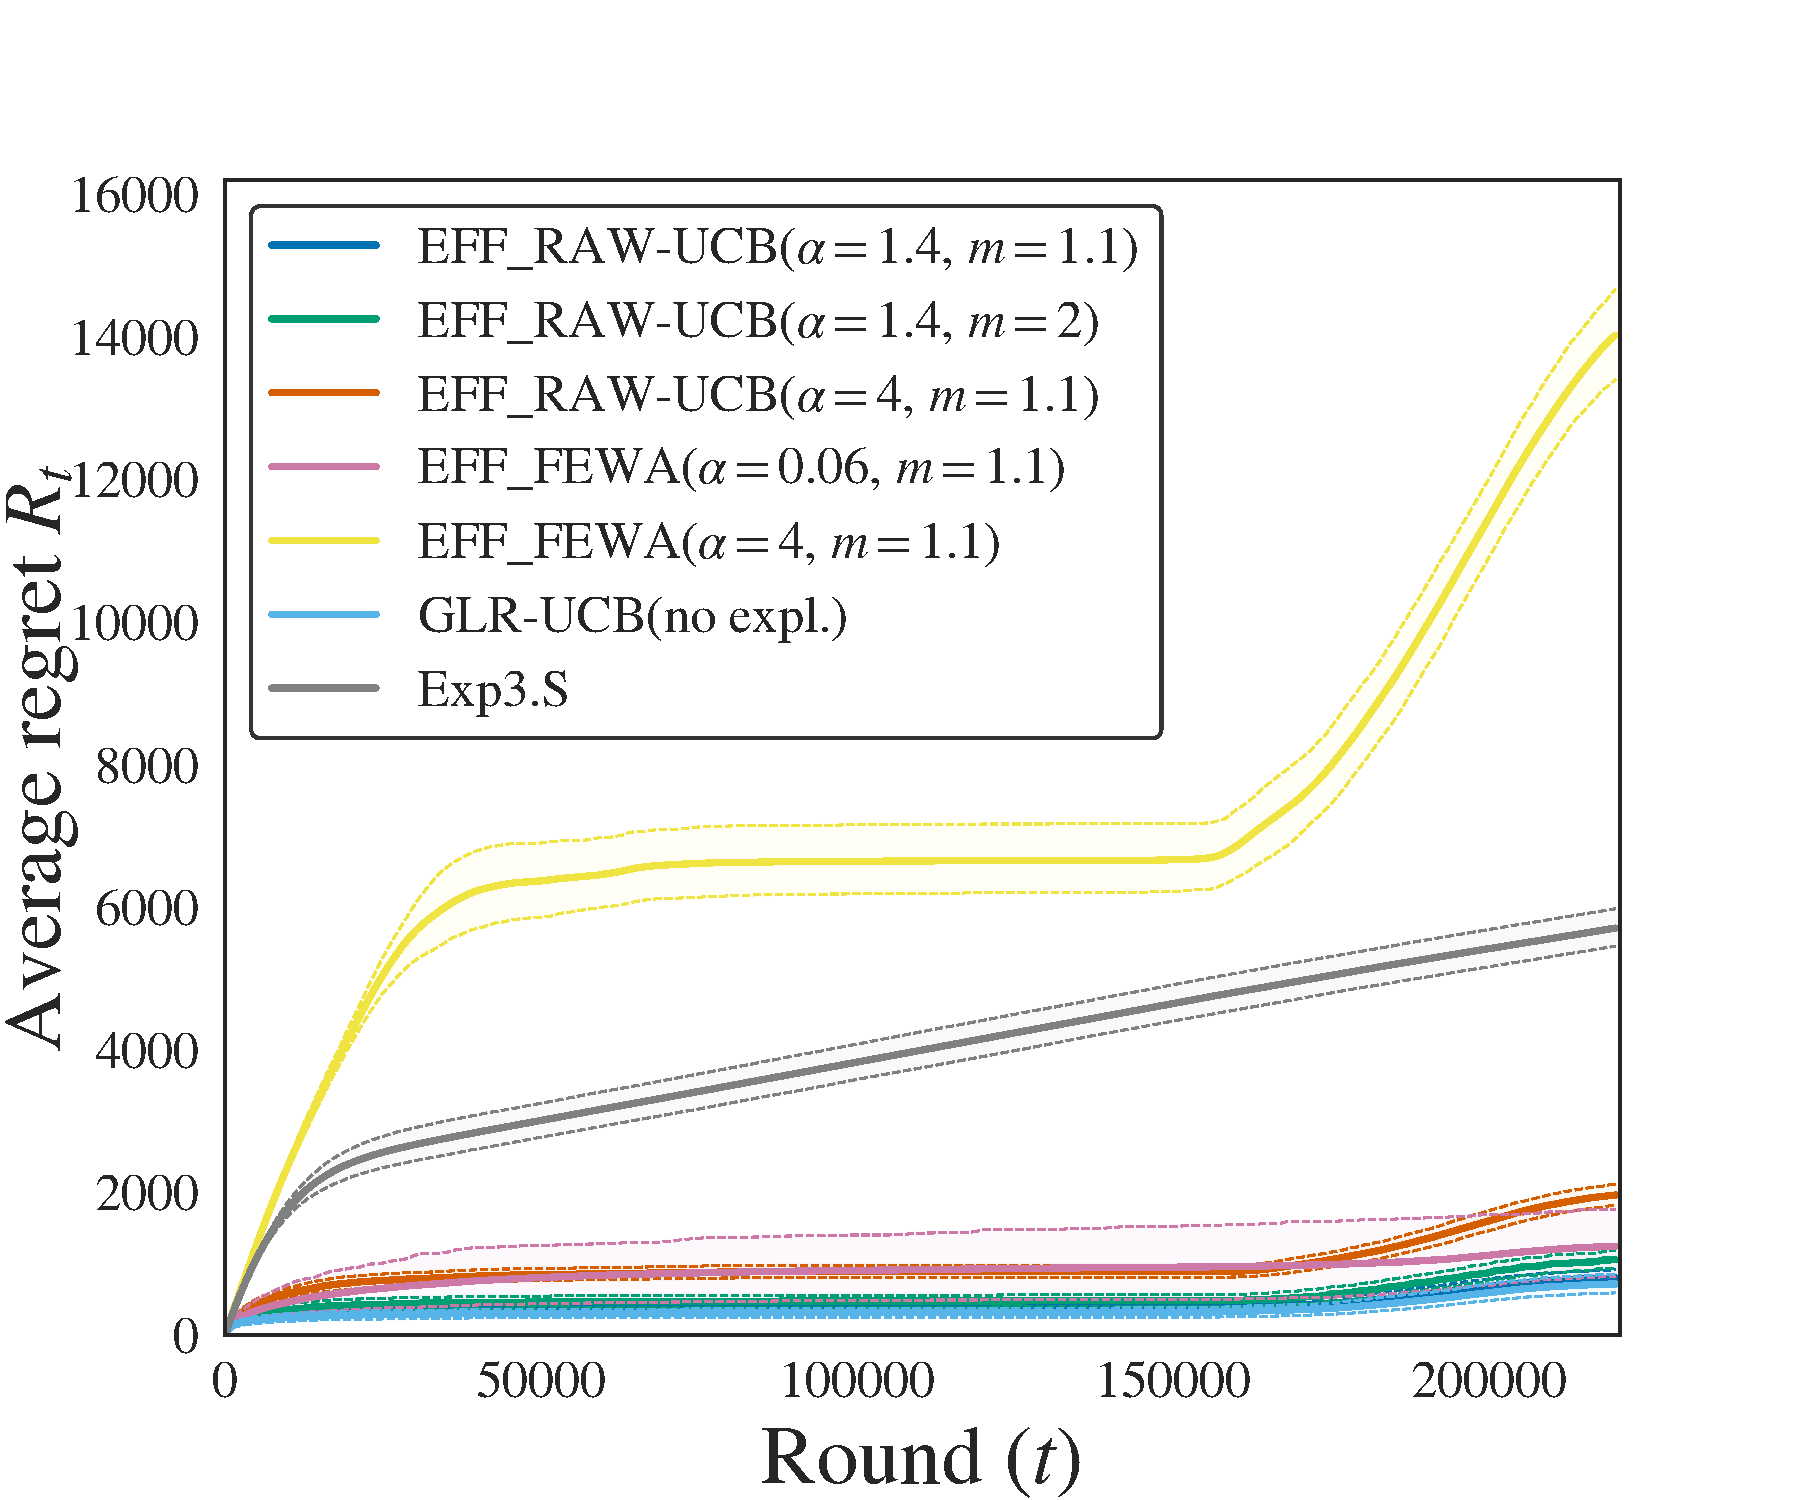
\includegraphics[clip, width= 0.495\textwidth]{4Restless/fig/DAY7.pdf}
\end{figure*}
\begin{figure*}[p!]
\includegraphics[clip, width= 0.495\textwidth]{4Restless/fig/reward_plot_day8.pdf}
\includegraphics[clip, width= 0.495\textwidth]{4Restless/fig/DAY8.pdf}
\includegraphics[clip, width= 0.495\textwidth]{4Restless/fig/reward_plot_day9.pdf}
\includegraphics[clip, width= 0.495\textwidth]{4Restless/fig/DAY9.pdf}
\includegraphics[clip, width= 0.495\textwidth]{4Restless/fig/reward_plot_day10.pdf}
\includegraphics[clip, width= 0.495\textwidth]{4Restless/fig/DAY10.pdf}
\end{figure*}
\begin{table*}[ht!]
\begin{center}
\begin{tabular}{|@{\hskip3pt}c@{\hskip3pt}|@{\hskip5pt}c@{\hskip5pt}|@{\hskip5pt}c@{\hskip5pt}|@{\hskip5pt}c@{\hskip5pt}|@{\hskip5pt}c@{\hskip5pt}|@{\hskip5pt}c@{\hskip5pt}|@{\hskip5pt}c@{\hskip5pt}|@{\hskip5pt}c@{\hskip5pt}|@{\hskip5pt}c@{\hskip5pt}|@{\hskip5pt}c@{\hskip5pt}|}
\hline
\textbf{Day} & \textbf{2} & \textbf{3} & \textbf{4} & \textbf{5} & \textbf{6} & \textbf{7} & \textbf{8} & \textbf{9}              & \textbf{10}               \\ \hline
\!\EFFRAW\! \footnotesize{$\!(\alpha\!=\!1.4, m\!=\!1.1)\!$} \!& 67         & 66         & 90         & 86         & 91         & 74         & 88         & 64 & 48 \\  
\!\EFFRAW\!  {\footnotesize$(\alpha\!=\!1.4, m\!=\!2)$} \!  & 35         & 33         & 43         & 47         & 46         & 41         & 44         & 34   & 45 \\  
\!\EFFRAW \!{\footnotesize $(\alpha\!=\!4, m\!=\!1.1)$}\!   & 65         & 65         & 90         & 88         & 91         & 74         & 89         & 63 & 48  \\ \hline
\EFFFEWA \footnotesize{$(\alpha\!=\!0.06)$}           & 143        & 175        & 223        & 159        & 183        & 115        & 193        & 116        &       165       \\ 
\EFFFEWA \footnotesize{$(\alpha\!=\!4)$}              & 337        & 308        & 391        & 473        & 487        & 380        & 428        & 341     &  388               \\ \hline 
\EXPS   & 56         & 53         & 67         & 77         & 75         & 69         & 71         & 55      &   78 \\ \hline
\GLRUCB  & 560        & 613        & 683        & 2421       & 707        & 1529       & 957        & 971  & 4017\\ \hline
\end{tabular}
  \caption{Average computational time in seconds for each algorithm in each experiment.}
  \label{tab:restless-time}
\end{center}
\end{table*}

\paragraph{{\RAWUCB} vs {\FEWA}.} The two algorithms compute the same statistics and share most of their analysis. Yet, {\RAWUCB} consistently outperforms {\FEWA} as it was the case on the rested benchmark. The difference between the two is even more significant in the restless case. Its theoretical tuning $\alpha = 4$ gets reasonable results, while theoretical {\FEWA} is impractical. Finally, its empirical tuning $\alpha_{\mathrm{R}} =1.4$ is similar to the asymptotic optimal tuning of {\UCB} and shows good performance on both rested and restless problems. By contrast, {\FEWA} with $\alpha_{\mathrm{F}} = 0.06$ shows worse performance with larger deviation on the restless benchmark. 

\paragraph{{\RAWUCB} vs {\EXPS}.} {\EXPS} has good performances on the restless benchmark, on which it has theoretical guarantees. Yet, it is consistently outperformed by {\RAWUCB} when we tune the confidence bounds. It is particularly true in easy instances, e.g. on day 7. Indeed, in these cases, we expect a logarithmic regret rate for {\RAWUCB}.

\paragraph{{\RAWUCB} vs {\GLRUCB} (no active exploration).}  On the restless benchmark, {\GLRUCB} shows similar results than {\RAWUCB}. Yet, we highlight that 1) {\GLRUCB} needs the knowledge of the horizon to tune its change-detector; 2) we use an efficient version of {\RAWUCB} which runs $\sim 10$ times faster than {\GLRUCB}. In fact, the two algorithms are similar: they are UCB index policies, they recover logarithmic rate on easy restless rotting bandits problems and hence they would both suffer near-linear worst-case regret rate in the general restless setting (when active exploration is turned off for {\GLRUCB}). The main difference is that {\RAWUCB} scans its history to select its rotting UCB's window, while {\GLRUCB} scans its history to detect significant changes and restart. 


%!TEX root = ../main.tex
\section{Restless and rested rotting bandits}
\label{sec:general_decreasing_MAB_framework}
\subsection{The general case}
\begin{assumption}\label{assum:general}
For each arm $i$, any number of pulls $n$, and time $t$, the functions $\mu_i(t,\cdot)$ and $\mu_i(\cdot,n)$ are non-increasing.
\end{assumption}

In Section~\ref{sec:restless-theory}, we highlight that the main guarantee of our algorithms - Lemma~\ref{lem:core-full} -  holds in the general case of Assumption~\ref{assum:general}. Is it enough to show that our algorithms are near-optimal in this extended setup?

Like in Chapter~\ref{ch:rested} and~\ref{ch:restless}, we define the regret with respect to the best oracle.
\begin{equation*}
R_T(\pi, \mu) \triangleq \argmax_{\pi^\star_T \in \PiO}  J_T(\pi^\star_T, \mu) - J_T(\pi).
\end{equation*}

Like in the linear rested rotting bandits (Section~\ref{sec:linear-rotting}), we can show that not only the greedy oracle suffers linear regret but no learning policy can get a sublinear regret rate in the worst-case. 

\begin{proposition}
\label{prop:general-rotting-unlearnable}
In the no noise setting ($\sigma = 0$), there exists a rotting 2-arms bandits problem (satisfying Assumption~\ref{assum:general}) with reward value in $\left[0,1\right]$, with one rested arm and one restless arm, and with at most one change-point before $T$ each, such that the greedy oracle strategy $\pi_O$ suffers a regret 
\[R_T\pa{\pi_O} \geq \floor{\frac{T}{4}}.\]
Moreover, for any learning strategy  $\pi_S$, there exists a rotting 2-arms bandits problem (satisfying Assumption~\ref{assum:general}) with reward value in $\left[0,1\right]$, with one rested arm and one restless arm, and with at most one change-point before $T$ each, such that 
\[R_T\pa{\pi_S} \geq \floor{\frac{T}{8}}.\]
\end{proposition}

Notice that the two reward functions of the constructed difficult problems are simple: either rested or restless, bounded, and with at most one break-point. If we consider a 2-arm setup with one rested arm and one restless arm, a good strategy may be to select the restless arm even when its current value is the worst. Indeed, this value is only available now, while the good value of the rested arm will still be available in the future. Whether the restless rewards are interesting to the learner depends on the future behavior of the (currently best) rested arm. On the first hand, if it decays below the current value of the restless arm before $T$ pulls, then the learner should profit from the restless reward available right now. On the other hand, if the rested arm stays optimal until the end of the game then the learner should ignore the restless arm and follows the greedy oracle strategy. However, the learner does not know in advance if (and how much) an arm will decay and any anticipation she makes will turn to be bad in the worst case. We formalize these ideas in the proof at the end of the section.

\subsection{Rested rotting bandits with a restless envelope}
\begin{assumption}
\label{assum:envelop}
We consider the following reward functions, 
\[
\mu_i(t,n) = P(t) f_i(n) + S(t),
\]
where $P: \NN^* \rightarrow \R_+$, $\left\{f_i : \NN \rightarrow \R\right\}_{i \in \arms}$ and $S: \NN^* \rightarrow \R$ are non-increasing functions. 
\end{assumption}

Notice that all the arms have the same product $P$ and sum $S$ functions, the only difference is the rested evolution $f_i$. That is why we call this setup the rested rotting bandits with a restless envelope.

With this assumption, we can show that the greedy oracle is optimal.
\begin{proposition}
\label{prop:envelop}
For any reward functions $\left\{\mu_i\right\}_{i \in \arms}$ verifying Assumption~\ref{assum:envelop} and any horizon $T$, $\GO \in \argmax_{\pi \in \PiO} J_T(\pi)$.
\end{proposition}

We leave as an open problem to analyze the aforementioned algorithms in this setup. A first step would be to characterize the performance of the greedy bandit policy in the absence of noise (as we did for the rested problem, see Subsection~\ref{ss:rested-noiseless-online}). We may not recover the $\cO\pa{K}$ bound as in the rested setup. Indeed, the adversary can use the variation of $P$ and $S$ to trick the greedy bandit policy several times for each arm. Moreover, the order of the pull do matter in this problem: the cumulative reward is not a function of $\left\{\NiT\right\}_{i \in \arms}$ anymore.

\subsection{Proofs}
\label{ss:rested-restless-proofs}
\begin{proof}[Proof of Proposition~\ref{prop:general-rotting-unlearnable}]
Let $\mu^{0}$ and $\mu^{1}$, two decreasing 2-arms bandits problems such that:
\begin{align*}
 &\mu^{0}_1(t,n) = \mu_1(n) = 1 \text{ if } n<\frac{T}{2} \text{ else } 0\,,\\
 &\mu^{1}_1(t,n) = 1\,, \\
 &\mu^{0}_2(t,n) = \mu^{1}_2(t,n) = \mu_2(t) = 1/2 \text{ if } t<\frac{T}{2} \text{ else } 0.
\end{align*}
Problem $\mu^{1}$ only evolves according to time. Hence, the oracle greedy policy $\pi_O$ is optimal for this problem and collects
\begin{equation}
\label{eq:regret1-piO}
J_T\pa{\pi_O, \mu^1} = T.
\end{equation}
On $\mu^{0}$, $\pi_O$ selects arm $1$ during $\floor{\frac{T}{2}}$ rounds and then both arms yield $0$ reward. Thus, $\pi_O$ collects 
\[J_T\pa{\pi_O, \mu^0} = \floor{\frac{T}{2}}.\]
However, let $\pi_0$ the policy which selects arm 2 for $\floor{\frac{T}{2}}$ rounds and arm 1 afterwards. Thus, $\pi_0$ collects
\begin{equation}
\label{eq:regret0-pi0}
  J_T\pa{\pi_0, \mu^0} = \pa{3/2} \floor{\frac{T}{2}}.  
\end{equation}
Hence, we conclude the first part of our proposition, 
\[R_T\pa{\pi_O, \mu^0} = J_T\pa{\pi^\star_T, \mu^0} - J_T\pa{\pi_O, \mu^0} \geq J_T\pa{\pi_0, \mu^0} - J_T\pa{\pi_O, \mu^0} \geq  \floor{\frac{T}{4}}.\]
Now, we consider any learning policy $\pi_S$ and we call $\EEempty_j\big[N_{i,t}(\pi_S)\big]$ the (expected, if the policy is random) number of pulls of arm $i$ at any round $t$ by $\pi_S$ on problem $j$. Note that the leaner will receive the same rewards for both problems until at least $\floor{\frac{T}{2}}$. Therefore, we have that 

\[ \forall t \leq \floor{\frac{T}{2}}, \pi\big(\mathcal{H}_t\pa{\mu^0}\big) = \pi\big(\mathcal{H}_t\pa{\mu^1}\big) \implies \EEempty_0\Big[N_{2,\floor{\frac{T}{2}}}(\pi_S)\Big] = \EEempty_1\Big[N_{2,\floor{\frac{T}{2}}}(\pi_S)\Big] \triangleq n_2.\]

On problem $\mu^{1}$, $\pi_S$ collects a reward of at most,
\begin{equation}
\label{eq:regret1-piS}
    J_T\pa{\pi_S, \mu^1} = \EEempty_1[N_{1,T}(\pi_S)] + \frac{n_2}{2} = T - \EEempty_1[N_{2,T}(\pi_S)] + \frac{n_2}{2} \leq T - \frac{n_2}{2}\CommaBin
\end{equation}
because $n_2 = \EEempty_1\Big[N_{2,\floor{\frac{T}{2}}}(\pi_S)\Big] \leq \EEempty_1[N_{2,T}(\pi_S)]$. Using Equations~\ref{eq:regret1-piO} and~\ref{eq:regret1-piS}, we can lower bound the regret of $\pi_S$, 
\[ R_T\pa{\pi_S, \mu^1} = J_T\pa{\pi_O, \mu^1} - J_T\pa{\pi_S, \mu^1} \geq  \frac{n_2}{2}\cdot \]


On problem $\mu^{0}$, $\pi_S$ collects a reward of at most,
\begin{equation}
\label{eq:regret0-piS}
    J_T\pa{\pi_S, \mu^0} = \min\pa{\EEempty_1[N_{1,T}(\pi_S)],\floor{\frac{T}{2}}} + \frac{n_2}{2} \leq \floor{\frac{T}{2}} + \frac{n_2}{2}\cdot
\end{equation}
Using Equations~\ref{eq:regret0-pi0} and~\ref{eq:regret0-piS}, we can lower bound the regret of $\pi_S$, 
\[ R_T\pa{\pi_S, \mu^0} = J_T\pa{\pi_O, \mu^0} - J_T\pa{\pi_S, \mu^0} \geq  \frac{\floor{T/2} - n_2}{2}\cdot \]

Hence, the worst case regret on the two setups is bounded by 
\[R_T(\pi_S) \geq \max\pa{\frac{n_2}{2}, \frac{\floor{\frac{T}{2}} - n_2}{2}} \geq \floor{\frac{T}{8}}\!\cdot \]
\end{proof}

\begin{proof}[Proof of Proposition~\ref{prop:envelop}]
At any round $t$, we have,
\[
\GO(t) \in \argmax_{i \in \arms} \pa{P(t)f_i(\Nit) + S(t)} = \argmax_{i \in \arms} f_i \pa{\Nit}.
\] 
Therefore, at round $t$, collects the $t$ largest values of $\ev{f_i(n)}_{i\in \arms, n\leq T}$, \textit{i.e.} 
\[
\forall i \in \arms, \ \forall n_i \geq \Nit, \ \mu_{\GO(t)}\pa{N_{\GO(t),\,t}} \geq\mu_{i}\pa{\Nit}  \geq \mu_i(n_i).
\]

The first inequality is due to the selection rule of the policy; the second is due to the decreasing reward functions. 

A direct consequence is that, at the round $t$, $\GO$ selects the $t$-th largest value of $\left\{f_i(n)\right\}_{i \in \arms, n \leq T}$. Hence, at the round $T$, it has selected the $T$ largest value in the decreasing order. Since $P(t)$ is non-increasing and positive, an other policy which selects smaller values of $\left\{f_i(n)\right\}_{i \in \arms, n \leq T}$, or the same values but in an other order, have a smaller or equal cumulative reward than $\GO$.
\end{proof}

\documentclass[12pt,fleqn]{book} % Default font size and left-justified equations

% !TEX root = main.tex


%%%%%%%%%%%%%%%%%%%%%%%%%%%%%%%%%%%%%%%%%
% The Legrand Orange Bookbookmarks=true,
% Structural Definitions File
% Version 2.0 (9/2/15)
%
% Original author:
% Mathias Legrand (legrand.mathias@gmail.com) with modifications by:
% Vel (vel@latextemplates.com)
% 
% This file has been downloaded from:
% http://www.LaTeXTemplates.com
%
% License:
% CC BY-NC-SA 3.0 (http://creativecommons.org/licenses/by-nc-sa/3.0/)
%
%%%%%%%%%%%%%%%%%%%%%%%%%%%%%%%%%%%%%%%%%

%----------------------------------------------------------------------------------------
%	VARIOUS REQUIRED PACKAGES AND CONFIGURATIONS
%----------------------------------------------------------------------------------------
\usepackage[top=3cm,bottom=3cm,left=3cm,right=3cm,headsep=10pt,a4paper]{geometry} % Page margins

\usepackage{graphicx} % Required for including pictures
\graphicspath{{fig/}} % Specifies the directory where pictures are stored

\usepackage{tikz} % Required for drawing custom shapes

%\usepackage[english]{babel} % English language/hyphenation

\usepackage{enumitem} % Customize lists
\setlist{nolistsep} % Reduce spacing between bullet points and numbered lists

\usepackage{booktabs} % Required for nicer horizontal rules in tables

\usepackage{xcolor} % Required for specifying colors by name
\definecolor{ocre}{RGB}{243,102,25} % Define the orange color used for highlighting throughout the book
\definecolor{myBlue}{RGB}{3,146,207} % Define the orange color used for highlighting throughout the book


%----------------------------------------------------------------------------------------
%	FONTS
%----------------------------------------------------------------------------------------

\usepackage{avant} % Use the Avantgarde font for headings
%\usepackage{times} % Use the Times font for headings
\usepackage{mathptmx} % Use the Adobe Times Roman as the default text font together with math symbols from the Sym­bol, Chancery and Com­puter Modern fonts

\usepackage{microtype} % Slightly tweak font spacing for aesthetics
\usepackage[utf8]{inputenc} % Required for including letters with accents
\usepackage[T1]{fontenc} % Use 8-bit encoding that has 256 glyphs

%----------------------------------------------------------------------------------------
%	BIBLIOGRAPHY AND INDEX
%----------------------------------------------------------------------------------------

\usepackage[style=authoryear-comp,uniquelist=false,citestyle=authoryear,sorting=ynt,sortcites=true,autopunct=true,babel=hyphen,hyperref,abbreviate=false,backref=true,backend=biber,maxcitenames=2,maxbibnames=20]{biblatex}
%\usepackage[style=authoryear-comp,citestyle=authoryear,sorting=nyt,sortcites=true,autopunct=true,babel=hyphen,hyperref,abbreviate=false,backref=true,backend=biber,maxcitenames=20]{biblatex}
\addbibresource{other_tex_files/PhD_Thesis_Julien_Seznec.bib} % BibTeX bibliography file
\defbibheading{bibempty}{}

\usepackage{calc} % For simpler calculation - used for spacing the index letter headings correctly
\usepackage{makeidx} % Required to make an index
\makeindex % Tells LaTeX to create the files required for indexing

%----------------------------------------------------------------------------------------
%	MAIN TABLE OF CONTENTS
%----------------------------------------------------------------------------------------

\usepackage{titletoc} % Required for manipulating the table of contents
%\usepackage{morewrites} % fix no room for new write error with tablecontent+listofalgorithms clash
\contentsmargin{0cm} % Removes the default margin

% Part text styling
\titlecontents{part}[0cm]
{\addvspace{20pt}\centering\large\bfseries}
{}
{}
{}

% Chapter text styling
\titlecontents{chapter}[1.25cm] % Indentation
{\addvspace{12pt}\large\sffamily\bfseries} % Spacing and font options for chapters
{\color{myBlue!60}\contentslabel[\Large\thecontentslabel]{1.25cm}\color{myBlue}} % Chapter number
{\color{myBlue}}  
{\color{myBlue!60}\normalsize\;\titlerule*[.5pc]{.}\;\thecontentspage} % Page number

% Section text styling
\titlecontents{section}[1.25cm] % Indentation
{\addvspace{3pt}\sffamily\bfseries} % Spacing and font options for sections
{\contentslabel[\thecontentslabel]{1.25cm}} % Section number
{}
{\hfill\color{black}\thecontentspage} % Page number
[]

% Subsection text styling
\titlecontents{subsection}[1.25cm] % Indentation
{\addvspace{1pt}\sffamily\small} % Spacing and font options for subsections
{\contentslabel[\thecontentslabel]{1.25cm}} % Subsection number
{}
{\ \titlerule*[.5pc]{.}\;\thecontentspage} % Page number
[]

% List of figures
\titlecontents{figure}[0em]
{\addvspace{-5pt}\sffamily}
{\thecontentslabel\hspace*{1em}}
{}
{\ \titlerule*[.5pc]{.}\;\thecontentspage}
[]

% List of tables
\titlecontents{table}[0em]
{\addvspace{-5pt}\sffamily}
{\thecontentslabel\hspace*{1em}}
{}
{\ \titlerule*[.5pc]{.}\;\thecontentspage}
[]

% List of algorithms
\titlecontents{algorithm}[0em]
{\addvspace{-5pt}\sffamily}
{\thecontentslabel\hspace*{1em}}
{}
{\ \titlerule*[.5pc]{.}\;\thecontentspage}
[]

%----------------------------------------------------------------------------------------
%	MINI TABLE OF CONTENTS IN PART HEADS
%----------------------------------------------------------------------------------------

% Chapter text styling
\titlecontents{lchapter}[0em] % Indenting
{\addvspace{15pt}\large\sffamily\bfseries} % Spacing and font options for chapters
{\color{myBlue}\contentslabel[\Large\thecontentslabel]{1.25cm}\color{myBlue}} % Chapter number
{}  
{\color{myBlue}\normalsize\sffamily\bfseries\;\titlerule*[.5pc]{.}\;\thecontentspage} % Page number

% Section text styling
\titlecontents{lsection}[0em] % Indenting
{\sffamily\small} % Spacing and font options for sections
{\contentslabel[\thecontentslabel]{1.25cm}} % Section number
{}
{}

% Subsection text styling
\titlecontents{lsubsection}[.5em] % Indentation
{\normalfont\footnotesize\sffamily} % Font settings
{}
{}
{}

%----------------------------------------------------------------------------------------
%	PAGE HEADERS
%----------------------------------------------------------------------------------------

\usepackage{fancyhdr} % Required for header and footer configuration

\pagestyle{fancy}
\renewcommand{\chaptermark}[1]{\markboth{\sffamily\normalsize\bfseries\chaptername\ \thechapter.\ #1}{}} % Chapter text font settings
\renewcommand{\sectionmark}[1]{\markright{\sffamily\normalsize\thesection\hspace{5pt}#1}{}} % Section text font settings
\fancyhf{} \fancyhead[LE,RO]{\sffamily\normalsize\thepage} % Font setting for the page number in the header
\fancyhead[LO]{\rightmark} % Print the nearest section name on the left side of odd pages
\fancyhead[RE]{\leftmark} % Print the current chapter name on the right side of even pages
\renewcommand{\headrulewidth}{0.5pt} % Width of the rule under the header
\addtolength{\headheight}{2.5pt} % Increase the spacing around the header slightly
\renewcommand{\footrulewidth}{0pt} % Removes the rule in the footer
\fancypagestyle{plain}{\fancyhead{}\renewcommand{\headrulewidth}{0pt}} % Style for when a plain pagestyle is specified

% Removes the header from odd empty pages at the end of chapters
\makeatletter
\renewcommand{\cleardoublepage}{
\clearpage\ifodd\c@page\else
\hbox{}
\vspace*{\fill}
\thispagestyle{empty}
\newpage
\fi}

%----------------------------------------------------------------------------------------
%	THEOREM STYLES
%----------------------------------------------------------------------------------------

\usepackage{amsmath,amsfonts,amssymb,amsthm} % For math equations, theorems, symbols, etc
\usepackage{environ}
\usepackage{thmtools}
\usepackage{thm-restate}
\AfterEndEnvironment{restatable}{\noindent\ignorespaces}
\newcommand{\intoo}[2]{\mathopen{]}#1\,;#2\mathclose{[}}
\newcommand{\ud}{\mathop{\mathrm{{}d}}\mathopen{}}
\newcommand{\intff}[2]{\mathopen{[}#1\,;#2\mathclose{]}}
\newtheorem{notation}{Notation}[chapter]

% Boxed/framed environments
\newtheoremstyle{ocrenumbox}% % Theorem style name
{10pt}% Space above
{0pt}% Space below
{\normalfont}% % Body font
{}% Indent amount
{\small\bf\sffamily\color{myBlue}}% % Theorem head font
{\;}% Punctuation after theorem head
{0.25em}% Space after theorem head
{\small\sffamily\color{myBlue}\thmname{#1}\nobreakspace\thmnumber{\@ifnotempty{#1}{}\@upn{#2}}% Theorem text (e.g. Theorem 2.1)
\thmnote{\nobreakspace\the\thm@notefont\sffamily\bfseries\color{black}---\nobreakspace#3.}} % Optional theorem note
\renewcommand{\qedsymbol}{$\blacksquare$}% Optional qed square

\newtheoremstyle{blacknumex}% Theorem style name
{10pt}% Space above
{0pt}% Space below
{\normalfont}% Body font
{} % Indent amount
{\small\bf\sffamily}% Theorem head font
{\;}% Punctuation after theorem head
{0.25em}% Space after theorem head
{\small\sffamily{\tiny\ensuremath{\blacksquare}}\nobreakspace\thmname{#1}\nobreakspace\thmnumber{\@ifnotempty{#1}{}\@upn{#2}}% Theorem text (e.g. Theorem 2.1)
\thmnote{\nobreakspace\the\thm@notefont\sffamily\bfseries---\nobreakspace#3.}}% Optional theorem note

\newtheoremstyle{blacknumbox} % Theorem style name
{0pt}% Space above
{0pt}% Space below
{\normalfont}% Body font
{}% Indent amount
{\small\bf\sffamily}% Theorem head font
{\;}% Punctuation after theorem head
{0.25em}% Space after theorem head
{\small\sffamily\thmname{#1}\nobreakspace\thmnumber{\@ifnotempty{#1}{}\@upn{#2}}% Theorem text (e.g. Theorem 2.1)
\thmnote{\nobreakspace\the\thm@notefont\sffamily\bfseries---\nobreakspace#3.}}% Optional theorem note

% Non-boxed/non-framed environments
\newtheoremstyle{ocrenum}% % Theorem style name
{5pt}% Space above
{5pt}% Space below
{\normalfont}% % Body font
{}% Indent amount
{\small\bf\sffamily\color{myBlue}}% % Theorem head font
{\;}% Punctuation after theorem head
{0.25em}% Space after theorem head
{\small\sffamily\color{myBlue}\thmname{#1}\nobreakspace\thmnumber{\@ifnotempty{#1}{}\@upn{#2}}% Theorem text (e.g. Theorem 2.1)
\thmnote{\nobreakspace\the\thm@notefont\sffamily\bfseries\color{black}---\nobreakspace#3.}} % Optional theorem note
\renewcommand{\qedsymbol}{$\blacksquare$}% Optional qed square
\makeatother

% Defines the theorem text style for each type of theorem to one of the three styles above
\newcounter{dummy} 
\numberwithin{dummy}{section}
\theoremstyle{ocrenumbox}
\newtheorem{theoremeT}[dummy]{Theorem}
\newtheorem{problem}{Problem}[chapter]
\newtheorem{exerciseT}{Exercise}[chapter]
\theoremstyle{blacknumex}
\newtheorem{exampleT}{Example}[chapter]
\theoremstyle{blacknumbox}
\newtheorem{vocabulary}{Vocabulary}[chapter]
\newtheorem{definitionT}{Definition}[section]
\newtheorem{corollaryT}[dummy]{Corollary}
\theoremstyle{ocrenum}
\newtheorem{proposition}[dummy]{Proposition}
\newtheorem{lemma}[dummy]{Lemma}
\newtheorem{assumption}[dummy]{Assumption}



%----------------------------------------------------------------------------------------
%	DEFINITION OF COLORED BOXES
%----------------------------------------------------------------------------------------

\RequirePackage[framemethod=default]{mdframed} % Required for creating the theorem, definition, exercise and corollary boxes

% Theorem box
\newmdenv[skipabove=2em,
skipbelow=7pt,
backgroundcolor=black!5,
linecolor=myBlue,
innerleftmargin=5pt,
innerrightmargin=5pt,
innertopmargin=5pt,
leftmargin=0cm,
rightmargin=0cm,
innerbottommargin=5pt]{tBox}

% Exercise box	  
\newmdenv[skipabove=7pt,
skipbelow=7pt,
rightline=false,
leftline=true,
topline=false,
bottomline=false,
backgroundcolor=myBlue!10,
linecolor=myBlue,
innerleftmargin=5pt,
innerrightmargin=5pt,
innertopmargin=5pt,
innerbottommargin=5pt,
leftmargin=0cm,
rightmargin=0cm,
linewidth=4pt]{eBox}	

% Definition box
\newmdenv[skipabove=2em,
skipbelow=7pt,
rightline=false,
leftline=true,
topline=false,
bottomline=false,
linecolor=myBlue,
innerleftmargin=5pt,
innerrightmargin=5pt,
innertopmargin=0pt,
leftmargin=0cm,
rightmargin=0cm,
linewidth=4pt,
innerbottommargin=0pt]{dBox}	

% Corollary box
\newmdenv[skipabove=2em,
skipbelow=7pt,
rightline=false,
leftline=true,
topline=false,
bottomline=false,
linecolor=gray,
backgroundcolor=black!5,
innerleftmargin=5pt,
innerrightmargin=5pt,
innertopmargin=15pt,
leftmargin=0cm,
rightmargin=0cm,
linewidth=4pt,
innerbottommargin=5pt]{cBox}

% Creates an environment for each type of theorem and assigns it a theorem text style from the "Theorem Styles" section above and a colored box from above
\newenvironment{theorem}{\begin{tBox}\begin{theoremeT}}{\end{theoremeT}\end{tBox}}
\newenvironment{exercise}{\begin{eBox}\begin{exerciseT}}{\hfill{\color{myBlue}\tiny\ensuremath{\blacksquare}}\end{exerciseT}\end{eBox}}				  
\newenvironment{definition}{\begin{dBox}\begin{definitionT}}{\end{definitionT}\end{dBox}}	
\newenvironment{example}{\begin{exampleT}}{\hfill{\tiny\ensuremath{\blacksquare}}\end{exampleT}}		
\newenvironment{corollary}{\begin{cBox}\begin{corollaryT}}{\end{corollaryT}\end{cBox}}
\makeatletter
% mnodified from page 3 of environ manual
\newcommand\wrap[1]{\begin{restatable}{theorem}{restapiecewisetheorem}#1\end{restatable}}
\newenvironment{restat}{\Collect@Body\wrap}{}
\makeatother			

%----------------------------------------------------------------------------------------
%	REMARK ENVIRONMENT
%----------------------------------------------------------------------------------------

\newenvironment{remark}{\par\vspace{0pt}\small % Vertical white space above the remark and smaller font size
\begin{list}{}{
\leftmargin=35pt % Indentation on the left
\rightmargin=25pt}\item\ignorespaces % Indentation on the right
\makebox[-2.5pt]{\begin{tikzpicture}[overlay]
\node[draw=myBlue!60,line width=1pt,circle,fill=myBlue!25,font=\sffamily\bfseries,inner sep=2pt,outer sep=0pt] at (-15pt,0pt){\textcolor{myBlue}{R}};\end{tikzpicture}} % Orange R in a circle
\advance\baselineskip -1pt}{\end{list}\vskip0pt} % Tighter line spacing and white space after remark

%----------------------------------------------------------------------------------------
%	SECTION NUMBERING IN THE MARGIN
%----------------------------------------------------------------------------------------

\makeatletter
\renewcommand{\@seccntformat}[1]{\llap{\textcolor{myBlue}{\csname the#1\endcsname}\hspace{1em}}}                    
\renewcommand{\section}{\@startsection{section}{1}{\z@}
{-4ex \@plus -1ex \@minus -.4ex}
{1ex \@plus.2ex }
{\normalfont\large\sffamily\bfseries}}
\renewcommand{\subsection}{\@startsection {subsection}{2}{\z@}
{-3ex \@plus -0.1ex \@minus -.4ex}
{0.5ex \@plus.2ex }
{\normalfont\sffamily\bfseries}}
\renewcommand{\subsubsection}{\@startsection {subsubsection}{3}{\z@}
{-2ex \@plus -0.1ex \@minus -.2ex}
{.2ex \@plus.2ex }
{\normalfont\small\sffamily\bfseries}}                        
%\renewcommand\paragraph{\@startsection{paragraph}{4}{\z@}
%{-2ex \@plus-.2ex \@minus .2ex}
%{.1ex}
%{\normalfont\small\sffamily\bfseries}}

%----------------------------------------------------------------------------------------
%	PART HEADINGS
%----------------------------------------------------------------------------------------

% numbered part in the table of contents
\newcommand{\@mypartnumtocformat}[2]{%
\setlength\fboxsep{0pt}%
\noindent\colorbox{myBlue!20}{\strut\parbox[c][.7cm]{\ecart}{\color{myBlue!70}\Large\sffamily\bfseries\centering#1}}\hskip\esp\colorbox{myBlue!40}{\strut\parbox[c][.7cm]{\linewidth-\ecart-\esp}{\Large\sffamily\centering#2}}}%
%%%%%%%%%%%%%%%%%%%%%%%%%%%%%%%%%%
% unnumbered part in the table of contents
\newcommand{\@myparttocformat}[1]{%
\setlength\fboxsep{0pt}%
\noindent\colorbox{myBlue!40}{\strut\parbox[c][.7cm]{\linewidth}{\Large\sffamily\centering#1}}}%
%%%%%%%%%%%%%%%%%%%%%%%%%%%%%%%%%%
\newlength\esp
\setlength\esp{4pt}
\newlength\ecart
\setlength\ecart{1.2cm-\esp}
\newcommand{\thepartimage}{}%
\newcommand{\partimage}[1]{\renewcommand{\thepartimage}{#1}}%
\def\@part[#1]#2{%
\ifnum \c@secnumdepth >-2\relax%
\refstepcounter{part}%
\addcontentsline{toc}{part}{\texorpdfstring{\protect\@mypartnumtocformat{\thepart}{#1}}{\partname~\thepart\ ---\ #1}}
\else%
\addcontentsline{toc}{part}{\texorpdfstring{\protect\@myparttocformat{#1}}{#1}}%
\fi%
\startcontents%
\markboth{}{}%
{\thispagestyle{empty}%
\begin{tikzpicture}[remember picture,overlay]%
\node at (current page.north west){\begin{tikzpicture}[remember picture,overlay]%	
\fill[myBlue!20](0cm,0cm) rectangle (\paperwidth,-\paperheight);
\node[anchor=north] at (4cm,-3.25cm){\color{myBlue!40}\fontsize{220}{100}\sffamily\bfseries\@Roman\c@part}; 
\node[anchor=south east] at (\paperwidth-1cm,-\paperheight+1cm){\parbox[t][][t]{8.5cm}{
\printcontents{l}{0}{\setcounter{tocdepth}{1}}%
}};
\node[anchor=north east] at (\paperwidth-1.5cm,-3.25cm){\parbox[t][][t]{15cm}{\strut\raggedleft\color{white}\fontsize{30}{30}\sffamily\bfseries#2}};
\end{tikzpicture}};
\end{tikzpicture}}%
\@endpart}
\def\@spart#1{%
\startcontents%
\phantomsection
{\thispagestyle{empty}%
\begin{tikzpicture}[remember picture,overlay]%
\node at (current page.north west){\begin{tikzpicture}[remember picture,overlay]%	
\fill[myBlue!20](0cm,0cm) rectangle (\paperwidth,-\paperheight);
\node[anchor=north east] at (\paperwidth-1.5cm,-3.25cm){\parbox[t][][t]{15cm}{\strut\raggedleft\color{white}\fontsize{30}{30}\sffamily\bfseries#1}};
\end{tikzpicture}};
\end{tikzpicture}}
\addcontentsline{toc}{part}{\texorpdfstring{%
\setlength\fboxsep{0pt}%
\noindent\protect\colorbox{myBlue!40}{\strut\protect\parbox[c][.7cm]{\linewidth}{\Large\sffamily\protect\centering #1\quad\mbox{}}}}{#1}}%
\@endpart}
\def\@endpart{\vfil\newpage
\if@twoside
\if@openright
\null
\thispagestyle{empty}%
\newpage
\fi
\fi
\if@tempswa
\twocolumn
\fi}

%----------------------------------------------------------------------------------------
%	CHAPTER HEADINGS
%----------------------------------------------------------------------------------------
\usepackage{varwidth}
\newcommand{\thechapterimage}{}%
\newcommand{\chapterimage}[1]{\renewcommand{\thechapterimage}{#1}}%
\def\@makechapterhead#1{%
{\parindent \z@ \raggedright \normalfont
\ifnum \c@secnumdepth >\m@ne
\if@mainmatter
\begin{tikzpicture}[remember picture,overlay]
\node at (current page.north west)
{\begin{tikzpicture}[remember picture,overlay]
\node[anchor=north west,inner sep=0pt] at (0,0) {\includegraphics[width=\paperwidth]{\thechapterimage}};
\draw[anchor=west] (\Gm@lmargin,-9cm) node [line width=2pt,rounded corners=15pt,draw=myBlue,fill=white,fill opacity=0.9,inner sep=5pt]{\strut\makebox[22cm][l]{\begin{minipage}{17cm}\huge\sffamily\bfseries\color{black}\thechapter. #1\end{minipage}\strut}};
%\draw[anchor=west] (\Gm@lmargin+.3cm,-9cm) node {\huge\sffamily\bfseries\color{black}\thechapter\autodot~#1\strut}
\end{tikzpicture}};
\end{tikzpicture}
\else
\begin{tikzpicture}[remember picture,overlay]
\node at (current page.north west)
{\begin{tikzpicture}[remember picture,overlay]
\node[anchor=north west,inner sep=0pt] at (0,0) {\includegraphics[width=\paperwidth]{\thechapterimage}};
\draw[anchor=west] (\Gm@lmargin,-9cm) node [line width=2pt,rounded corners=15pt,draw=myBlue,fill=white,fill opacity=0.9,inner sep=15pt]{\strut\makebox[22cm]{}};
\draw[anchor=west] (\Gm@lmargin+.3cm,-9cm) node {\huge\sffamily\bfseries\color{black}#1\strut};
\end{tikzpicture}};
\end{tikzpicture}
\fi\fi\par\vspace*{270\p@}}}

%-------------------------------------------

\def\@makeschapterhead#1{%
\begin{tikzpicture}[remember picture,overlay]
\node at (current page.north west)
{\begin{tikzpicture}[remember picture,overlay]
\node[anchor=north west,inner sep=0pt] at (0,0) {\includegraphics[width=\paperwidth]{\thechapterimage}};
\draw[anchor=west] (\Gm@lmargin,-9cm) node [line width=2pt,rounded corners=15pt,draw=myBlue,fill=white,fill opacity=0.9,inner sep=15pt]{\strut\makebox[22cm]{}};
\draw[anchor=west] (\Gm@lmargin+.3cm,-9cm) node {\huge\sffamily\bfseries\color{black}#1\strut};
\end{tikzpicture}};
\end{tikzpicture}
\par\vspace*{270\p@}}
\makeatother

%----------------------------------------------------------------------------------------
%	HYPERLINKS IN THE DOCUMENTS
%----------------------------------------------------------------------------------------

\usepackage[colorlinks=true,
            linkcolor=myBlue,
            urlcolor=blue,
            citecolor=gray]{hyperref}
\hypersetup{hidelinks,colorlinks=true,breaklinks=true,urlcolor= myBlue,bookmarksopen=false,pdftitle={Bandits for Intelligent Tutoring System},pdfauthor={Julien Seznec}} %backref=true,pagebackref=true,hyperindex=true,bookmarks=true,
%TODO SET Title
\usepackage{bookmark}
\bookmarksetup{
open,
numbered,
addtohook={%
\ifnum\bookmarkget{level}=0 % chapter
\bookmarksetup{bold}%
\fi
\ifnum\bookmarkget{level}=-1 % part
\bookmarksetup{color=myBlue,bold}%
\fi
}
}
\usepackage{amsthm}
\usepackage{amsmath}
\usepackage{amssymb}
\usepackage{bbm}
\usepackage{thm-restate}
\usepackage{nicefrac}       % compact symbols for 1/2, etc.x
\usepackage[htt]{hyphenat}
\AfterEndEnvironment{restatable}{\noindent\ignorespaces}
\usepackage{bm}
\usepackage{dsfont}
% !TEX root = main.tex

\DeclareMathOperator*{\argmax}{arg\,max}
\DeclareMathOperator*{\argmin}{arg\,min}
\DeclareMathOperator*{\arginf}{arg\,inf}
\DeclareMathOperator*{\sgn}{sgn}
%\DeclareMathOperator{\regret}{regret}
\DeclareMathOperator{\polylog}{polylog}
\DeclareMathOperator{\logloglog}{logloglog}
\DeclareMathOperator{\polyloglog}{polyloglog}


\newcommand*\diff{\mathop{}\!\mathrm{d}}
\newcommand*\Diff[1]{\mathop{}\!\mathrm{d^#1}}
\renewcommand{\d}[1]{\ensuremath{\operatorname{d}\!{#1}}}

\newcommand{\set}[1]{\left\{#1\right\}}
%\DeclarePairedDelimiter\ceil{\lceil}{\rceil}
%\DeclarePairedDelimiter\floor{\lfloor}{\rfloor}
\newcommand{\ceil}[1]{\left\lceil#1\right\rceil}
\newcommand{\floor}[1]{\left\lfloor#1\right\rfloor}

%\newcommand{\ceil}[1]{\lceil#1\rceil}

\newcommand{\II}[1]{\mathds{1}_{\left\{#1\right\}}}
\newcommand{\I}{{\mathds{1}}}


%arrows 
\newcommand{\ra}{\rightarrow}

%distributions 
\newcommand{\Bernoulli}{\mathrm{Bernoulli}}


\newcommand{\specialcell}[2][c]{%
 \begin{tabular}[#1]{@{}c@{}}#2\end{tabular}}

\newtheorem{assumption}{Assumption}
%\newtheorem{lemma}{Lemma}
%\newtheorem{theorem}{Theorem}
%\newtheorem{definition}{Definition}
%\newtheorem{corollary}{Corollary}
%\newtheorem{remark}{Remark}


% \newcommand{\R}{I\!\! R}
\newcommand{\R}{\mathbb{R}}
\newcommand{\realset}{\mathbb{R}}

\newcommand{\NN}{{\mathbb N}}
\newcommand{\1}{\mathds{1}}
\newcommand{\bOne}{{\bf 1}}
\newcommand{\bZero}{{\bf 0}}
\newcommand{\E}{\mathbb{E}}
\newcommand{\EE}[1]{\mathbb{E}\left[#1\right]}
\newcommand{\EEt}[1]{\mathbb{E}_t\left[#1\right]}
\newcommand{\EEs}[2]{\mathbb{E}_{#1}\left[#2\right]}
\newcommand{\EEc}[2]{\mathbb{E}\left[#1\left|#2\right.\right]}
\newcommand{\EEcc}[2]{\mathbb{E}\left[\left.#1\right|#2\right]}
\newcommand{\EEcct}[2]{\mathbb{E}_t\left[\left.#1\right|#2\right]}
\newcommand{\PP}[1]{\mathbb{P}\left[#1\right]}
\newcommand{\PPt}[1]{\mathbb{P}_t\left[#1\right]}
 \newcommand{\PPc}[2]{\mathbb{P}\left[#1\left|#2\right.\right]}
\newcommand{\PPcc}[2]{\mathbb{P}\left[\left.#1\right|#2\right]}
\newcommand{\PPct}[2]{\mathbb{P}_t\left[#1\left|#2\right.\right]}
\newcommand{\PPcct}[2]{\mathbb{P}_t\left[\left.#1\right|#2\right]}
\newcommand{\EEempty}{\mathbb{E}}
\newcommand{\PPempty}{\mathbb{P}}
%parens
\newcommand{\pa}[1]{\left(#1\right)}
\newcommand{\sqpa}[1]{\left[#1\right]}
\newcommand{\ac}[1]{\left\{#1\right\}}
\newcommand{\ev}[1]{\left\{#1\right\}}
\newcommand{\card}[1]{\left|#1\right|}


\newcommand{\normtwo}[1]{\|#1\|_2}
\newcommand{\norm}[1]{\left\|#1\right\|}
\newcommand{\onenorm}[1]{\norm{#1}_1}
\newcommand{\infnorm}[1]{\norm{#1}_\infty}

\newcommand{\abs}[1]{\left|#1\right|}

\newcommand*{\MyDef}{\mathrm{\tiny def}}
\newcommand*{\eqdefU}{\ensuremath{\mathop{\overset{\MyDef}{=}}}}% Unscaled version
\newcommand*{\eqdef}{\mathop{\overset{\MyDef}{\resizebox{\widthof{\eqdefU}}{\heightof{=}}{=}}}}
%\newcommand{\eqdef}{\stackrel{{\rm def}}{=}}
%\newcommand{\eqdef}{\stackrel{{\rm \tiny def}}{=}}
\newcommand{\transpose}{^\mathsf{\scriptscriptstyle T}}

%Calligraphic Shorthands
\newcommand{\cA}{\mathcal{A}}
\newcommand{\cB}{\mathcal{B}}
\newcommand{\cC}{\mathcal{C}}
\newcommand{\cD}{\mathcal{D}}
\newcommand{\cE}{\mathcal{E}}
\newcommand{\F}{\mathcal{F}}
\newcommand{\cF}{\mathcal{F}}
\newcommand{\cG}{\mathcal{G}}
\newcommand{\cH}{\mathcal{H}}
\newcommand{\cI}{\mathcal{I}}
\newcommand{\cJ}{\mathcal{J}}
\newcommand{\cK}{\mathcal{K}}
\newcommand{\cL}{\mathcal{L}}
\newcommand{\calL}{\cL}
\newcommand{\cM}{\mathcal{M}}
\newcommand{\cN}{\mathcal{N}}
\newcommand{\cO}{\mathcal{O}}
\newcommand{\tcO}{\widetilde{\cO}}
\newcommand{\OO}{\mathcal{O}}
\newcommand{\tOO}{\wt{\OO}}
\newcommand{\cP}{\mathcal{P}}
\newcommand{\cQ}{\mathcal{Q}}
\newcommand{\cR}{\mathcal{R}}
\newcommand{\Sw}{\mathcal{S}}
\newcommand{\cS}{\mathcal{S}}
\newcommand{\cT}{\mathcal{T}}
\newcommand{\T}{\cT}
\newcommand{\cU}{\mathcal{U}}
\newcommand{\cV}{\mathcal{V}}
\newcommand{\cW}{\mathcal{W}}
\newcommand{\cX}{\mathcal{X}}
\newcommand{\X}{\cX}
\newcommand{\cY}{\mathcal{Y}}
\newcommand{\cZ}{\mathcal{Z}}

%Bolds Shorthands
\newcommand{\bA}{{\bf A}}
\newcommand{\bb}{{\bf b}}
\newcommand{\bB}{{\bf B}}
\newcommand{\bc}{{\bf c}}
\newcommand{\bC}{{\bf C}}
\newcommand{\bD}{{\bf D}}
\newcommand{\bg}{{\bf g}}
\newcommand{\bG}{{\bf G}}
\newcommand{\bI}{{\bf I}}
\newcommand{\bM}{{\bf M}}
\newcommand{\bO}{\boldsymbol{O}}
\newcommand{\bp}{\boldsymbol{p}}
\newcommand{\bP}{{\bf P}}
\newcommand{\br}{{\bf r}}
\newcommand{\bR}{{\bf R}}
\newcommand{\bQ}{{\bf Q}}
\newcommand{\be}{{\bf e}}
\newcommand{\bff}{{\bf f}}
\newcommand{\bi}{{\bf i}}
\newcommand{\bk}{{\bf k}}
\newcommand{\bK}{{\bf K}}
\newcommand{\bL}{{\bf L}}
\newcommand{\bs}{{\bf s}}
\newcommand{\bq}{{\bf q}}
\newcommand{\bu}{{\bf u}}
\newcommand{\bU}{{\bf U}}
\newcommand{\bv}{{\bf v}}
\newcommand{\bV}{{\bf V}}
\newcommand{\bw}{{\bf w}}
\newcommand{\bW}{{\bf W}}
\newcommand{\by}{{\bf y}}
\newcommand{\bx}{{\bf x}}
\newcommand{\bX}{{\bf X}}
\newcommand{\bZ}{{\bf Z}}

\newcommand{\eps}{\varepsilon}
\renewcommand{\epsilon}{\varepsilon}
\renewcommand{\hat}{\widehat}
\renewcommand{\tilde}{\widetilde}
\renewcommand{\bar}{\overline}

\newcommand{\balpha}{{\boldsymbol \alpha}}
\newcommand{\talpha}{\widetilde{\indn}}
\newcommand{\btheta}{{\boldsymbol \theta}}
\newcommand{\tTheta}{{\widetilde\Theta}}
\newcommand{\bdelta}{{\boldsymbol \delta}}
\newcommand{\bDelta}{{\boldsymbol \Delta}}
\newcommand{\bLambda}{{\boldsymbol \Lambda}}
\newcommand{\bSigma}{{\boldsymbol \Sigma}}
\newcommand{\Bmu}{{\boldsymbol \mu}}
\newcommand{\bxi}{{\boldsymbol \xi}}
\newcommand{\bell}{\boldsymbol \ell}

\newcommand{\nothere}[1]{}
\newcommand{\moveb}{\\ \bigskip}

% bandits
\newcommand{\hloss}{\hat\ell}
\newcommand{\bloss}{\boldsymbol  \ell}
\newcommand{\hbl}{\hat{\bloss}}
\newcommand{\hbL}{\wh{\bL}}
\newcommand{\wh}{\widehat}
\newcommand{\ti}{_{t,i}}
\newcommand{\wt}{\widetilde}



%% from single papers, but merged here
% algo names
\usepackage{xspace}
\renewcommand{\ttdefault}{lmtt}
%other algos
\newcommand{\LP}{\texttt{LP}\xspace}
\newcommand{\CMG}{\texttt{CMG}\xspace}
%bandits
\newcommand{\FPL}{\texttt{FPL}\xspace}
\newcommand{\TS}{\texttt{TS}\xspace}
\newcommand{\UCB}{\texttt{UCB}\xspace}
\newcommand{\MOSS}{\texttt{MOSS}\xspace}
\newcommand{\UCBE}{\texttt{UCB-E}\xspace}
\newcommand{\ImprovedUCB}{\texttt{ImprovedUCB}\xspace}
\newcommand{\klucb}{\texttt{KL-UCB}\xspace}
\newcommand{\CUCB}{\texttt{CUCB}\xspace}
\newcommand{\EXP}{\texttt{Exp3}\xspace}
\newcommand{\exph}{\EXP}
%linear bandits
\newcommand{\LinearTS}{\texttt{LinearTS}\xspace}
\newcommand{\ThompsonSampling}{\texttt{ThompsonSampling}\xspace}
\newcommand{\SpectralEliminator}{\texttt{\textcolor[rgb]{0.5,0.2,0}{SpectralEliminator}}\xspace}
\newcommand{\LinearEliminator}{\texttt{\textcolor[rgb]{0.5,0.2,0}{LinearEliminator}}\xspace}
\newcommand{\LinUCB}{\texttt{LinUCB}\xspace}
\newcommand{\LinRel}{\texttt{LinRel}\xspace}
\newcommand{\KernelUCB}{\texttt{\textcolor[rgb]{0.5,0.2,0}{KernelUCB}}\xspace}
\newcommand{\SupKernelUCB}{\texttt{\textcolor[rgb]{0.5,0.2,0}{SupKernelUCB}}\xspace}
\newcommand{\GPUCB}{\texttt{GP-UCB}\xspace}
\newcommand{\OFUL}{\texttt{OFUL}\xspace}
\newcommand{\OPM}{\texttt{\textcolor[rgb]{0.5,0.2,0}{OPM}}\xspace}
%graph bandits
\newcommand{\CLUB}{\texttt{CLUB}\xspace}
\newcommand{\GOBLin}{\texttt{GOB.Lin}\xspace}
\newcommand{\UCBN}{\texttt{UCB-N}\xspace}
\newcommand{\UCBmaxN}{\texttt{UCB-MaxN}\xspace}
\newcommand{\GraphMOSS}{\texttt{\textcolor[rgb]{0.5,0.2,0}{GraphMOSS}}\xspace}
\newcommand{\SpectralUCB}{\texttt{\textcolor[rgb]{0.5,0.2,0}{SpectralUCB}}\xspace}
\newcommand{\CheapUCB}{\texttt{\textcolor[rgb]{0.5,0.2,0}{CheapUCB}}\xspace}
\newcommand{\SpectralTS}{\texttt{\textcolor[rgb]{0.5,0.2,0}{SpectralTS}}\xspace}
\newcommand{\SupLinRel}{\texttt{SupLinRel}\xspace}
\newcommand{\SupLinUCB}{\texttt{SupLinUCB}\xspace}
\newcommand{\imb}{\texttt{\textcolor[rgb]{0.5,0.2,0}{IMLinUCB}}\xspace}
\newcommand{\NetBandits}{\texttt{NetBandits}\xspace}
\newcommand{\BARE}{\texttt{\textcolor[rgb]{0.5,0.2,0}{BARE}}\xspace}
\newcommand{\ELP}{\texttt{ELP}\xspace}
\newcommand{\ELPP}{\texttt{ELP.P}\xspace}
\newcommand{\expix}{\texttt{\textcolor[rgb]{0.5,0.2,0}{Exp3-IX}}\xspace}
\newcommand{\expset}{\texttt{Exp3-SET}\xspace}
\newcommand{\expdom}{\texttt{Exp3-DOM}\xspace}
\newcommand{\expg}{\texttt{Exp3.G}\xspace}
\newcommand{\fplbgr}{\texttt{FPL-BGR}\xspace}
\newcommand{\fplix}{\texttt{\textcolor[rgb]{0.5,0.2,0}{FPL-IX}}\xspace}
\newcommand{\comphedge}{\texttt{Component\-Hedge}\xspace}
\newcommand{\hedge}{\texttt{Hedge}\xspace}
\newcommand{\expxxx}{\texttt{\textcolor[rgb]{0.5,0.2,0}{Exp3-WIX}}\xspace}
\newcommand{\expwix}{\texttt{\textcolor[rgb]{0.5,0.2,0}{Exp3-WIX}}\xspace}
\newcommand{\expixa}{\texttt{Exp3-IXa}\xspace}
\newcommand{\expixb}{\texttt{Exp3-IXb}\xspace}
\newcommand{\expixt}{\texttt{Exp3-IXt}\xspace}
\newcommand{\expcoop}{\texttt{Exp3-Coop}\xspace}
\newcommand{\expres}{\texttt{\textcolor[rgb]{0.5,0.2,0}{Exp3-Res}}\xspace}

%continuous bandits
\newcommand{\StoSOO}{\texttt{\textcolor[rgb]{0.5,0.2,0}{StoSOO}}\xspace}
\newcommand{\POO}{\texttt{\textcolor[rgb]{0.5,0.2,0}{POO}}\xspace}
\newcommand{\DOO}{\texttt{DOO}\xspace}
\newcommand{\SOO}{\texttt{SOO}\xspace}
\newcommand{\Zooming}{\texttt{Zooming}\xspace}
\newcommand{\UCT}{\texttt{UCT}\xspace}
\newcommand{\HCT}{\texttt{HCT}\xspace}
\newcommand{\SHOO}{\POO}
\newcommand{\HOO}{\texttt{HOO}\xspace}
\newcommand{\ATB}{\texttt{ATB}\xspace}
\newcommand{\TZ}{\texttt{TaxonomyZoom}\xspace}
\newcommand{\Direct}{\texttt{DiRect}\xspace}
%extreme bandits
\newcommand{\SiRI}{\texttt{\textcolor[rgb]{0.5,0.2,0}{SiRI}}\xspace}
%planning "bandits"
\newcommand{\olop}{\texttt{OLOP}\xspace}
\newcommand{\stopalgo}{\texttt{StOP}\xspace}
\newcommand{\metagrill}{\texttt{\textcolor[rgb]{0.5,0.2,0}{TrailBlazer}}\xspace}
%polymatroid bandits
\newcommand{\greedy}{\texttt{Greedy}\xspace}
\newcommand{\opm}{\texttt{\textcolor[rgb]{0.5,0.2,0}{OPM}}\xspace}


\newcommand{\maxn}{\texttt{max}\xspace}
\newcommand{\avgn}{\texttt{avg}\xspace}


%kernelUCB
\newcommand{\reg}{\gamma}
\newcommand{\hmu}{\hat{\mu}}
\newcommand{\bmu}{\bar{\mu}}
%\newcommand{\hm}{\hat{\mu}}
\newcommand{\hw}{\hat{w}}
\newcommand{\hth}{\hat{\theta}}
\newcommand{\hs}{\hat{\sigma}}
\newcommand{\hepsilon}{\hat{\epsilon}}


%graph bandit notation
\newcommand{\etat}{\eta_t}
\newcommand{\gammat}{\gamma_t}
\newcommand{\nodes}{{\textcolor[rgb]{0.3,0.8,0.0}{N}}}
\newcommand{\rounds}{{\textcolor[rgb]{0.3,0.0,0.8}{T}}}
\newcommand{\td}{{\textcolor[rgb]{0.6,0.0,0.6}{\tilde{d}}}}
\newcommand{\matL}{{\textcolor[rgb]{0.6,0.0,0.6}{L}}}
\newcommand{\matK}{{\textcolor[rgb]{0.6,0.0,0.6}{K}}}
\newcommand{\effd}{{\textcolor[rgb]{0.6,0.0,0.6}{d}}}
\newcommand{\effD}{{\textcolor[rgb]{0.6,0.0,0.6}{D}}}
\newcommand{\indn}{{\textcolor[rgb]{0.6,0.0,0.6}{\alpha}}}
\newcommand{\indnstar}{{\textcolor[rgb]{0.6,0.0,0.6}{\alpha^\star}}}
\newcommand{\cliquen}{{\textcolor[rgb]{0.6,0.0,0.6}{\chi}}}
\newcommand{\erdosr}{{\textcolor[rgb]{0.6,0.0,0.6}{r}}}
\newcommand{\detD}{{\textcolor[rgb]{0.6,0.0,0.6}{D}}}
\newcommand{\detDstar}{{\textcolor[rgb]{0.6,0.0,0.6}{D_\star}}}
\newcommand{\infibeta}{{\textcolor[rgb]{0.6,0.0,0.6}{\beta}}}
\newcommand{\mas}{{\textcolor[rgb]{0.6,0.0,0.6}{\texttt{mas}}}}
\newcommand{\nodeset}{\cV}
\newcommand{\edgeset}{\cE}
\newcommand{\regret}{R_\rounds}
\newcommand{\cgamma}{c_\gamma}
\newcommand{\cgammat}{c_{\gamma_t}}
\newcommand{\sumT}{\sum_{t = 1}^\rounds}
\newcommand{\sumt}{\sum_{t=1}^\rounds}
\newcommand{\sumtl}{\sum\limits_{t=1}^\rounds}
\newcommand{\sumj}{\sum_{j\in \nodes_i^-}}
\newcommand{\sumtj}{\sum_{j\in \nodes_{t,i}^-}}
\newcommand{\sumi}{\sum_{i=1}^{\nodes}}
\newcommand{\sumji}{\sum_{j\in \{\nodes_i^-\cup\{i\}\}}}
\newcommand{\sumtji}{\sum_{j\in \{\nodes_{t,i}^-\cup\{i\}\}}}
\newcommand{\dti}{d_{t,i}^-}
\newcommand{\hdi}{\hat{d}_i^-}
\newcommand{\hdk}{\hat{d}_k^-}
\newcommand{\hd}{\hat{d}^-}
\newcommand{\tti}{_{t+1,i}}
\newcommand{\tj}{_{t,j}}
\newcommand{\ji}{_{j,i}}
\newcommand{\Ii}{_{I_t,i}}
\newcommand{\pti}{p\ti}
\newcommand{\pta}{p_{t,a}}
\newcommand{\qti}{q\ti}
\newcommand{\hpti}{\hat{p}\ti}
\newcommand{\hpi}{\hat{p}_i}
\newcommand{\hp}{\hat{p}}
\newcommand{\hqti}{\hat{q}\ti}
\newcommand{\ptj}{p_{t,j}}
\newcommand{\qtj}{q_{t,j}}
\newcommand{\hptj}{\hat{p}_{t,j}}
\newcommand{\hqtj}{\hat{q}_{t,j}}
\newcommand{\oti}{o\ti}
\newcommand{\Oti}{O\ti}
\newcommand{\loss}{\ell}
\newcommand{\hLoss}{\hat{L}}
\newcommand{\hL}{\wh{L}}
\newcommand{\noise}{\epsilon}
%spectral
\newcommand{\dold}{\effd_{\scriptsize\mbox{old}}}
\newcommand{\dnew}{\effd_{\scriptsize\mbox{new}}}
%wix
\newcommand{\gweight}{s}
\newcommand{\avgalpha}{\indnstar_{\text{avg}}}
%bare
\newcommand{\rkdual}{r_k^{\circ}}
\newcommand{\rktdual}{r_{k,t}^{\circ}}
\newcommand{\rkprimetdual}{r_{k',t}^{\circ}}
\newcommand{\rkttdual}{r_{k,t+1}^{\circ}}
\newcommand{\rkprimettdual}{r_{k',t+1}^{\circ}}
\newcommand{\ridual}{r_i^{\circ}}
\newcommand{\rstardual}{r_\star^{\circ}}
\newcommand{\Ddual}{D^{\circ}}
\newcommand{\Ddualset}{\mathcal D^{\circ}}
%continuous bandit notation
%\newcommand{\node}[2]{\circ[#1,#2]}
\newcommand{\node}[2]{(#1,#2)}
\newcommand{\CommaBin}{\mathbin{\raisebox{0.5ex}{,}}}


%%% todos
\usepackage[colorinlistoftodos, textwidth=30mm, shadow, textsize=small]{todonotes}
\definecolor{babyblue}{rgb}{0.54, 0.81, 0.94}
\definecolor{citrine}{rgb}{0.89, 0.82, 0.04}
\definecolor{misocolor}{rgb}{0.16,0.27,0.86}
\newcommand{\todom}[1]{\todo[color=misocolor!30]{#1}\xspace}
\newcommand{\todomi}[1]{\todo[inline,color=misocolor!30]{#1}}
\newcommand{\wb}[1]{\overline{#1}}



\newcommand{\ind}{\mathbb{I}}
\newcommand{\narms}{K}
\newcommand{\currentTime}{t}
\newcommand{\lipschitz}{L}
\newcommand{\timeEnd}{T}
\newcommand{\currentNumPull}{N_{\pi(t)}(t)}
\newcommand{\numPullEnd}{N_{\pi(T}(T)}
\newcommand{\rewardFunction}{r^i}
\newcommand{\subgaussian}{\sigma}
\newcommand{\arm}{i}
\newcommand{\armCount}{N}
\newcommand{\policy}{\pi}
\newcommand{\reward}{\mu}
\newcommand{\obs}{o}
\newcommand{\totalReward}{J}
\newcommand{\expectation}{\mathop{\mathbb{E}}}
\newcommand{\possibleArms}{\mathcal{K}}
\newcommand{\arms}{\mathcal{K}}
\newcommand{\window}{h}
\newcommand{\estReward}{\hat{\reward}}
\newcommand{\expestReward}{\bar{\reward}}
\newcommand{\historyt}{\mathcal{H}_\currentTime}
\newcommand{\history}{\mathbf{H}}
\newcommand{\historyn}{\mathcal{H}_\timeEnd}
\newcommand{\underpullSet}{\textsc{up}}
\newcommand{\overpullSet}{\textsc{op}}
\newcommand{\HPevent}{\xi^\alpha_t}
\newcommand{\HPeff}{\xi^\alpha_{t,\, \texttt{eff}}}
\newcommand{\HPSWA}{\xi_{\rm SWA}}
\newcommand{\policySet}{\Pi}
\newcommand{\rewardSet}{\mathcal{L}_L}
\newcommand{\BBxSet}{\mathcal{B}_{B,x}}
\newcommand{\BBSet}{\mathcal{B}_{B}}
\newcommand{\BSet}{\mathcal{B}}
\newcommand{\stationarySet}{\mathcal{S}_L}
\newcommand{\myAlgorithm}{\normalfont \texttt{FEWA}\xspace}

\newcommand{\GO}{\pi_{\rm O}}
\newcommand{\Azero}{\mathcal{A}_{\rm 0}}
\newcommand{\Atwo}{\mathcal{A}_{\rm 2}}
\newcommand{\GB}{\pi_{\rm G}}
\newcommand{\FEWA}{\normalfont \texttt{FEWA}\xspace}
\newcommand{\EWA}{\policy_{\rm F}}
\newcommand{\piF}{\policy_{\rm F}}
\newcommand{\wSWA}{\normalfont \texttt{wSWA}\xspace}
\newcommand{\SWA}{\normalfont \texttt{SWA}\xspace}
\newcommand{\piSWA}{\pi_{\rm SWA}}

\newcommand{\DUCB}{\normalfont \texttt{D-UCB}\xspace}
\newcommand{\SWUCB}{\normalfont \texttt{SW-UCB}\xspace}
\newcommand{\UCBone}{\normalfont \texttt{UCB1}\xspace}
\newcommand{\EFF}{\normalfont {\texttt{EFF\_UPDATE}}\xspace}
\newcommand{\EFFP}{\policy_{\rm EFF-FEWA}}
\newcommand{\FILTER}{\normalfont \texttt{FILTER}\xspace}
\newcommand{\UPDATE}{\normalfont \texttt{UPDATE}\xspace}
\newcommand{\EFFFEWA}{\normalfont \texttt{EFF-FEWA}\xspace}
\newcommand{\EUCB}{\normalfont \texttt{RAW-UCB}\xspace}
\newcommand{\XUCB}{\normalfont \texttt{RAW-UCB}\xspace}
\newcommand{\RUCB}{\normalfont \texttt{RAW-UCB}\xspace}
\newcommand{\RAW}{\normalfont \texttt{RAW-UCB}\xspace}
\newcommand{\piX}{\policy_{\rm R}}
\newcommand{\piR}{\policy_{\rm R}}
\newcommand{\EFFU}{\normalfont \texttt{EFF-RAW-UCB}\xspace}
\newcommand{\EFFX}{\normalfont \texttt{EFF-RAW-UCB}\xspace}
\newcommand{\EFFRAW}{\normalfont \texttt{EFF-RAW-UCB}\xspace}
\newcommand{\piEFFE}{\normalfont \policy_{\rm ERUCB}\xspace}
\newcommand{\piEXU}{\normalfont \policy_{\rm ERUCB}\xspace}
\newcommand{\piEFFR}{\normalfont \policy_{\rm ERUCB}\xspace}
\newcommand{\piER}{\normalfont \policy_{\rm ER}\xspace}
\newcommand{\piEF}{\normalfont \policy_{\rm EF}\xspace}
\newcommand{\EFFKLR}{\normalfont \texttt{EFF-kl-RAW-UCB}\xspace}
\newcommand{\EXPS}{\normalfont \texttt{Exp3.S}\xspace}
\newcommand{\EXPR}{\normalfont \texttt{Exp3.R}\xspace}
\newcommand{\ADSWITCH}{\normalfont \texttt{AdSwitch}\xspace}
\newcommand{\GLRKLUCB}{\normalfont \texttt{GLR-klUCB}\xspace}
\newcommand{\GLRUCB}{\normalfont \texttt{GLR-UCB}\xspace}
\newcommand{\MUCB}{\normalfont \texttt{M-UCB}\xspace}
\newcommand{\CUSUMUCB}{\normalfont \texttt{CUSUM-UCB}\xspace}
\newcommand{\ADAILTCBplus}{\normalfont \texttt{ADA-ILTCB+}\xspace}

\newcommand{\PiO}{\Pi_{\rm O}}
\newcommand{\PiL}{\Pi_{\rm L}}
\newcommand{\Nit}{N_{i,\,t}}
\newcommand{\Nitmone}{N_{i,\,t-1}}
\newcommand{\NiT}{N_{i,\,T}}
\newcommand{\Njt}{N_{j,\,t}}
\newcommand{\Njtmone}{N_{j,\,t-1}}
\newcommand{\NjT}{N_{j,\,T}}
\newcommand{\Nitpi}{N_{i,\,t}^\pi}
\newcommand{\Nitmonepi}{N_{i,\,t-1}^\pi}
\newcommand{\NiTpi}{N_{i,\,T}^\pi}
\newcommand{\Njtpi}{N_{j,\,t}^\pi}
\newcommand{\Njtmonepi}{N_{j,\,t-1}^\pi}
\newcommand{\NjTpi}{N_{j,\,T}^\pi}
\newcommand{\hit}{h_{i,\,t}}
\newcommand{\hitmone}{h_{i,\,t-1}}
\newcommand{\hiT}{h_{i,\,T}}
\newcommand{\hjt}{h_{j,\,t}}
\newcommand{\hjtmone}{h_{j,\,t-1}}
\newcommand{\hjT}{h_{j,\,T}}
\newcommand{\hitpi}{h_{i,\,t}^\pi}
\newcommand{\hiTpi}{h_{i,\,T}^\pi}
\newcommand{\hjtpi}{h_{j,\,t}^\pi}
\newcommand{\hjTpi}{h_{j,\,T}^\pi}
\newcommand{\PPv}{\mathbb{P}}
\newcommand{\ie}{\emph{i.e.}\xspace} 
\newcommand{\piFRSet}{\left\{\piF, \piR\right\}}
\newcommand{\Him}{H_{i,\,m}}
\newcommand{\Hitm}{H_{i_t,\,m}}
\newcommand{\hmueff}{\hmu_{i,\texttt{eff}}^{h_j}}
\newcommand{\hmuiteff}{\hmu_{i_t,\texttt{eff}}^{h_j}}
\newcommand{\bmueff}{\bmu_{i,\texttt{eff}}^{h_j}}
\newcommand{\bmuiteff}{\bmu_{i_t,\texttt{eff}}^{h_j}}
\newcommand{\neff}{n_i^{h_j}}
\newcommand{\peff}{p_i^{h_j}}
\newcommand{\ist}{i^\star_t}
\newcommand{\tteff}{\texttt{eff}}


\usepackage{algorithmicx}
\usepackage{algorithm,algpseudocode}
\usepackage{footnote}
\usepackage{subcaption}
\usepackage{float}
\usepackage{wrapfig}
\usepackage{afterpage}
\usepackage{placeins}
\usepackage{svg}
\newcommand{\bookboxx}[1]{\small
\par\medskip\noindent
\framebox[0.46\textwidth]{
\begin{minipage}{0.44\dimexpr\textwidth-\parindent\relax} {#1} \end{minipage} } \par\medskip }

\setlength\parindent{0pt}
\setlength\parskip{1em plus 2pt}
%\setlength{\parskip}{1em}

\newcommand{\citep}{\parencite}
\newcommand{\citet}{\textcite}
\hypersetup{pdftitle={Thèse de Doctorat, Julien SEZNEC},pdfauthor={Julien SEZNEC}}


\begin{document}
\newpage
~\vfill
\thispagestyle{empty}
{\fontfamily{ptm}\selectfont 

 \vspace{-3cm} \hspace{-1cm}\fbox{
\begin{minipage}[c]{16cm}
\vspace{.2cm}
\begin{center}
{\large\sc\bf\sffamily TH\`ESE DE DOCTORAT DE L'UNIVERSIT\'E DE LILLE} 
\\{\bf {\sffamily École Doctorale Sciences Pour l'Ingénieur}}\\
{\sffamily Sp{\'e}cialit{\'e} :} {\bf\sffamily Informatique}

\vspace{.2cm}
\end{center}
\end{minipage}
}

%\vspace{1.0cm}
%\begin{center}
%  \includegraphics[width=0.2\columnwidth]{fig/ens.pdf}
%  %\hspace{5cm}
%  %\includegraphics[width=0.18\columnwidth]{fig/inria.pdf}
%\end{center}
%\vspace{0.5cm}

\begin{center}
{\sffamily \vspace{.4cm} Thèse de Doctorat pr\'esent\'ee par \vspace{.4cm}}

{\large \bf\sffamily  Julien SEZNEC} \\
\end{center}

\vspace{.4cm}
\begin{center}
\hspace{-0.3cm}\hrulefill \hspace{.2cm}

\vspace{.2cm}

\hspace{-.5cm}{\bf \Large \sffamily{Sequential Machine Learning for Adaptive Educational Systems}}

\vspace{-.1cm}

\hspace{-0.3cm}\hrulefill \\ \hspace{.2cm}

{\sffamily
sous la direction de MM. Michal Valko et Alessandro Lazaric, \\ et l'encadrement de M. Jonathan Banon.
}
\end{center}



\vspace{1.cm}

{\sffamily

\begin{tabular}{lllll}
{\bf\sffamily Rapporteurs :} 
& {M.}   & Aur\' elien & {\bf\sffamily GARIVIER} & ENS de Lyon \\
& {M.}   & Gilles & {\bf\sffamily STOLTZ}     & Universit\'e Paris Saclay \& CNRS \\
\end{tabular}

{\sffamily\vspace{1.cm} Soutenue le {\bf\sffamily 15 décembre 2020} devant le jury
compos{\'e} de}
}
\bigskip

\bigskip

%\hspace{-1.5cm}
{\sffamily
\begin{tabular}{llllll}
 {M.}   & Gilles & {\bf\sffamily STOLTZ}     & Univ. Paris Saclay \& CNRS & Rapporteur\\
{M.}   & Aur\' elien & {\bf\sffamily GARIVIER} & ENS de Lyon & Rapporteur \\
{M.}   & Steffen & {\bf\sffamily GRÜNEWÄLDER}     &  University of Lancaster & Examinateur\\
{M.}   & Manuel & {\bf\sffamily LOPES}     &  Instituto Superior Tecnico & Examinateur\\
{Mme}   & Mathilde & {\bf\sffamily MOUGEOT}     & Univ. Paris Saclay \& ENSIEE & Examinatrice\\
{M.}   & Michal & {\bf\sffamily VALKO}     &  INRIA Lille \& Deepmind & Directeur\\
{M.}   & Alessandro & {\bf\sffamily LAZARIC}     &  INRIA Lille \& FAIR  & Co-Directeur\\
{M.}   & Jonathan & {\bf\sffamily BANON}     &  Lelivrescolaire.fr & Encadrant\\
\end{tabular}
}
\begin{center}
\small\sffamily{Centre de Recherche en Informatique, Signal et Automatique de Lille (CRIStAL),\\
UMR 9189 Équipe SequeL, 59650, Villeneuve d’Ascq, France}
\end{center}
\makebox[\textwidth][c]{
\includegraphics[width=0.36\columnwidth]{fig/logo_lls.pdf}
\includegraphics[width=0.288\columnwidth]{fig/logo_univ-lille.png}
\includegraphics[width=0.264\columnwidth]{fig/logo_cristal.pdf}
\includegraphics[width=0.288\columnwidth]{fig/logo_inria.pdf}
}
%!TEX root = ./main.tex
\cleardoublepage
\hspace{0pt}
\vfill
\begin{flushright}
\emph{À mes grands-parents: Denise, Jean et Germaine}.
\end{flushright}
\vfill
\hspace{0pt}
\cleardoublepage
\section*{R\'esum\'e}
Proposer des séquences adaptatives d'exercices dans un Environnement informatique pour l'Apprentissage Humain (EIAH) nécessite de caractériser les lacunes de l'élève et d'utiliser cette caractérisation dans une stratégie pédagogique adaptée. Puisque les élèves ne font que quelques dizaines de questions dans une session de révision, ces deux objectifs sont en compétition. L'apprentissage automatique appelle \emph{problème de bandits} ces dilemmes d'exploration-exploitation dans les prises de décisions séquentielles. Dans cette thèse, nous étudions trois problèmes de bandits pour une application dans les systèmes éducatifs adaptatifs.

Les \emph{bandits décroissants au repos} sont un problème de décision séquentiel dans lequel la récompense associée à une action décroît lorsque celle-ci est sélectionnée. Cela modélise le cas où un élève progresse quand il travaille et l'EIAH cherche à sélectionner le sujet le moins maîtrisé pour combler les plus fortes lacunes. Nous présentons de nouveaux algorithmes et nous montrons que pour un horizon inconnu $T$ et sans aucune connaissance sur la décroissance des $K$ bras, ces algorithmes atteignent une borne de regret dépendante du problème $\cO(\log{T}),$ et une borne indépendante du problème $\tcO(\sqrt{KT})$. Nos résultats améliorent substantiellement l'état de l'art, ou seule une borne minimax $\tcO(K^{\nicefrac{1}{3}}T^{\nicefrac{2}{3}})$ avait été atteinte. Ces nouvelles bornes sont à des facteurs polylog des bornes optimales sur le problème stationnaire, donc nous concluons: les bandits décroissants ne sont pas plus durs que les bandits stationnaires.

Dans les \emph{bandits décroissants sans repos}, la récompense peut décroître à chaque tour pour toutes les actions. Cela modélise des situations différentes telles que le vieillissement du contenu dans un système de recommandation. On montre que les algorithmes conçus pour le problème "au repos" atteignent les bornes inférieures agnostiques au problème et une borne dépendante du problème $\cO(\log{T})$. Cette dernière est inatteignable dans le cas général ou la récompense peut croître. Nous concluons : l'hypothèse de décroissance simplifie l'apprentissage des bandits sans repos. 

Viser le sujet le moins connu peut être intéressant avant un examen, mais pendant le cursus - quand tous les sujets ne sont pas bien compris - cela peut mener à l'échec de l'apprentissage de l'étudiant. On étudie un Processus de Décision Markovien Partiellement Observable (POMDP, selon l'acronyme anglais) dans lequel on cherche à maîtriser le plus de sujets le plus rapidement possible. On montre que sous des hypothèses raisonnables sur l'apprentissage de l'élève, la meilleure stratégie oracle sélectionne le sujet le plus connu sous le seuil de maîtrise. Puisque cet oracle optimal n'a pas besoin de connaitre la dynamique de transition du POMDP, nous proposons une stratégie apprenante avec des outils "bandits" classiques, en évitant ainsi les méthodes gourmandes en données de l'apprentissage de POMDP.
\newpage

\section*{Abstract}
Designing an adaptive sequence of exercises in Intelligent Tutoring Systems (ITS) requires to characterize the gaps of the student and to use this characterization in a relevant pedagogical strategy. Since a student does no more than a few tens of exercises in a session, these two objectives compete. Machine learning called these exploration-exploitation trade-offs in sequential decision making the \emph{bandits problems}. In this thesis, we study different bandits setups for intelligent tutoring systems.%TODO

The \emph{rested rotting bandits} are a sequential decision problem in which the reward associated with an action may decrease when it is selected. It models the situation where the student improves when he works and the ITS aims the least known subject to fill the most important gaps.  We design new algorithms and we prove that for an unknown horizon $T$, and without any knowledge on the decreasing behavior of the $K$ arms, these algorithms achieve problem-dependent regret bound of $\cO(\log{T}),$ and a problem-independent one of $\tcO(\sqrt{KT})$. Our result substantially improves over existing algorithms, which suffers minimax regret $\tcO(K^{\nicefrac{1}{3}}T^{\nicefrac{2}{3}})$. These bounds are at a polylog factor of the optimal bounds on the classical stationary bandit; hence our conclusion: rotting bandits are not harder than stationary ones. 

In the \emph{restless rotting bandits}, the reward may decrease at each round for all the actions. They model different situations such as the obsolescence of content in recommender systems. We show that the rotting algorithms designed for the rested case match the problem-independent lower bounds and a $\cO(\log{T})$ problem-dependent one. The latter was shown to be unachievable in the general case where rewards can increase. We conclude: the rotting assumption makes the restless bandits easier.

Targeting the least known topic may be interesting before an exam but during the curriculum - when all the subjects are not yet understood - it can lead to failure in the learning of the student. We study a Partially Observable Markov Decision Process in which we aim at mastering as many topics as fast as possible. We show that under relevant assumptions on the learning of the student, the best oracle policy targets the most known topic under the mastery threshold. Since this optimal oracle does not need to know the transition dynamics of the POMDP, we design a learning policy with classical bandits tools, hence avoiding the data-intensive methods of POMDP learning. 
\newpage

\section*{Acknowledgments}
Je remercie Aurélien Garivier et Gilles Stoltz pour leurs relectures de cette version du manuscrit. Je n'ignore pas la quantité de travail que cela représente, et je suis sincèrement touché qu'ils aient accepté d'être Rapporteurs.

I also would like to thank the examiners - Mathilde Mougeot, Manuel Lopes, and Steffen Grünewälder -  for accepting my invitation.

More acknowledgments to come in the final version.

\cleardoublepage
\chapterimage{chapter_head/0_content.jpg} % Table of contents heading image

\pagestyle{empty} % Disable headers and footers for the following pages

\tableofcontents % Print the table of contents itself
\chapterimage{chapter_head/0_figures.jpg}
% list of items
\begingroup
\makeatletter
\chapter*{List of items}
\section*{Figures}
\@starttoc{lof}
\let\clearpage\relax
%\listoftables
\section*{Tables}
\@starttoc{lot}
\section*{Algorithms}
\@starttoc{loa}
\makeatother
\endgroup


\cleardoublepage % Forces the first chapter to start on an odd page so it is not on the right side of the book

\pagestyle{fancy} % Enable headers and footers again

%%----------------------------------------------------------------------------------------
%%	GLOSSARY
%%----------------------------------------------------------------------------------------
%\clearpage
%
%\printglossary[numberedsection,type=symbols,style=list,nogroupskip]
%
%%\printglossary[type=\acronymtype, style=myList]
%\printglossary[type=\acronymtype]
%\printglossaries
\clearpage
%!TEX root = ../main.tex
\part{Introduction}
\input{2Literature/0Afterclasse}
\input{2Literature/1Bandits}
\input{2Literature/2ITS}


%!TEX root = ../main.tex
\part{Rotting bandits}
\section*{Decreasing reward}
In Subsection~\ref{ss:less-known}, we presented a line of work that aims at asking questions from the least known subject to a student. In the multi-armed bandits' formulation, it associates positive reward to failed questions. Yet, none of these works consider the impact of the questions on the knowledge of the student. When the answer is given to the student after her trial, questions are a powerful learning tool. Therefore, the more the student work on a topic, the better he becomes, and the smaller is the reward for this topic.

Other situations can be modeled with decreasing rewards caused by the repetition of an action. For instance, the more we recommend an item to a user in a recommender system, the more he might get bored \citep{warlop2018fighting}. In medicine, the efficiency of antibiotics is diminishing with the overall use due to bacteria's mutation \citep{ventola2015antibiotic, ventola2015antibiotic2}.

In microeconomics, the law of diminishing marginal utility states that the utility associated with each unit of goods is decreasing with the number of goods a consumer holds. It is an \emph{ad hoc} explanation to justify that rational consumers, who maximize their total utility, may select different goods. In production theory, the law of diminishing returns \citep{canan1892origin} states that the increment of production caused by the increment of a factor of production (labor, capital) by one unit is decreasing. Again, there is the idea that repeating always the same action - buying one good, investing in a project - may become suboptimal even though the returns were high at the beginning. 

Motivated by these broad applications, \citet{heidari2016tight, levine2017rotting} study this non-stationarity with bandits feedback.  \citet{heidari2016tight} study the noise-less case under the name \emph{decaying bandits}. \citet{levine2017rotting} study the problem with noise under the name \emph{rotting bandits}. In the following, we call this problem the \emph{rested rotting bandits} to emphasize that actions cause the rewards' decay. We also mention the works of \citet{warlop2018fighting, immorlica2018recharging, pikeburke2019recovering} which model boredom effects in recommender systems as a rested decaying bandit problem but with restless recharging effects. 

In Chapter~\ref{ch:rested}, we synthesized our contributions to the rested rotting bandits problem\citep{seznec2019rotting, seznec2020single}: we present new algorithms and we prove that for an unknown horizon $T$, and without any knowledge on the decreasing behavior of the $K$ arms, these algorithms achieve problem-dependent regret bound of $\tcO(\log{(T)}),$ and a problem-independent one of $\tcO(\sqrt{KT})$. Our result substantially improves over the algorithm of~\citet{levine2017rotting}, which suffers regret $\tcO(K^{1/3}T^{2/3})$. These bounds are at a polylog factor of the optimal bounds on the stationary problem; hence our conclusion: rotting bandits are not harder than stationary ones. 

Another decaying setup is when the reward decreases no matter what the agent is doing. It models different situations such as the aging of content in recommender systems. \citet{louedec2016algorithme} models obsolescence of appearing arms (e.g. piece of news) with a known exponential rate. \cite{komiyama2014time-decaying} study a parametric decay in restless bandits where rewards are linear combinations of known decaying functions. However, the rotting assumption was not studied in the well-studied non-parametric restless bandit setting\citep{garivier2011upper-confidence-bound, auer2019adaptively,chen2019new, cheung2019new, russac2019weighted, besson2019generalized, liu2018change-detection, cao2019nearly, besbes2014stochastic}. That is why we consider the  \emph{restless rotting bandits} problem in Chapter~\ref{ch:restless} which is adapted from \citet{seznec2020single}.  We show that the rotting algorithms designed for the rested case match the problem-independent lower bound and a problem-dependent $\cO(\log{T})$. The latter was shown to be unachievable in the general case where rewards can increase. We conclude: the rotting assumption makes the restless bandits easier. 

Since the same algorithms work in both setups, we investigate in Section~\ref{sec:general_decreasing_MAB_framework} the joint setup where the reward can decrease with the number of pulls and the rounds. Yet, we show that the optimal oracle policy cannot be approached at a nontrivial rate by a learning policy.

\chapterimage{chapter_head/4_94tag.jpg} 
\chapter{Rested rotting bandits are not harder than stationary ones}
\label{ch:rested}
\vspace{-3cm}
\begin{flushright}
\emph{This rested rotting bandit seems quite stationary to me.}
\end{flushright}
\vspace{.85cm}
\input{3Rested/2Model}
\input{3Rested/3Algorithm}
\input{3Rested/4Theory}
\input{3Rested/5Simulation}
\input{3Rested/6Efficient}
\input{3Rested/7HowHarder}
\input{3Rested/8Linear}

%!TEX root = ../main.tex
\chapterimage{chapter_head/5_361Sarajevo.jpg} 
\chapter{The rotting assumption makes restless bandits easier}
\label{ch:restless}
\vspace{-3cm}
\begin{flushright}
\emph{A non-rotting restless bandit. Who would say he is not tough?}
\end{flushright}
\vspace{.85cm}
\input{4Restless/1Restless}
\input{4Restless/2Theory}
\input{4Restless/3Experiment}
\input{4Restless/4RestedRestless}
\documentclass[12pt,fleqn]{book} % Default font size and left-justified equations

\input{structure}
\usepackage{amsthm}
\usepackage{amsmath}
\usepackage{amssymb}
\usepackage{bbm}
\usepackage{thm-restate}
\usepackage{nicefrac}       % compact symbols for 1/2, etc.x
\usepackage[htt]{hyphenat}
\AfterEndEnvironment{restatable}{\noindent\ignorespaces}
\usepackage{bm}
\usepackage{dsfont}
\input{szsymbols}
\usepackage{algorithmicx}
\usepackage{algorithm,algpseudocode}
\usepackage{footnote}
\usepackage{subcaption}
\usepackage{float}
\usepackage{wrapfig}
\usepackage{afterpage}
\usepackage{placeins}
\usepackage{svg}
\newcommand{\bookboxx}[1]{\small
\par\medskip\noindent
\framebox[0.46\textwidth]{
\begin{minipage}{0.44\dimexpr\textwidth-\parindent\relax} {#1} \end{minipage} } \par\medskip }

\setlength\parindent{0pt}
\setlength\parskip{1em plus 2pt}
%\setlength{\parskip}{1em}

\newcommand{\citep}{\parencite}
\newcommand{\citet}{\textcite}
\hypersetup{pdftitle={Thèse de Doctorat, Julien SEZNEC},pdfauthor={Julien SEZNEC}}


\begin{document}
\newpage
~\vfill
\thispagestyle{empty}
{\fontfamily{ptm}\selectfont 

 \vspace{-3cm} \hspace{-1cm}\fbox{
\begin{minipage}[c]{16cm}
\vspace{.2cm}
\begin{center}
{\large\sc\bf\sffamily TH\`ESE DE DOCTORAT DE L'UNIVERSIT\'E DE LILLE} 
\\{\bf {\sffamily École Doctorale Sciences Pour l'Ingénieur}}\\
{\sffamily Sp{\'e}cialit{\'e} :} {\bf\sffamily Informatique}

\vspace{.2cm}
\end{center}
\end{minipage}
}

%\vspace{1.0cm}
%\begin{center}
%  \includegraphics[width=0.2\columnwidth]{fig/ens.pdf}
%  %\hspace{5cm}
%  %\includegraphics[width=0.18\columnwidth]{fig/inria.pdf}
%\end{center}
%\vspace{0.5cm}

\begin{center}
{\sffamily \vspace{.4cm} Thèse de Doctorat pr\'esent\'ee par \vspace{.4cm}}

{\large \bf\sffamily  Julien SEZNEC} \\
\end{center}

\vspace{.4cm}
\begin{center}
\hspace{-0.3cm}\hrulefill \hspace{.2cm}

\vspace{.2cm}

\hspace{-.5cm}{\bf \Large \sffamily{Sequential Machine Learning for Adaptive Educational Systems}}

\vspace{-.1cm}

\hspace{-0.3cm}\hrulefill \\ \hspace{.2cm}

{\sffamily
sous la direction de MM. Michal Valko et Alessandro Lazaric, \\ et l'encadrement de M. Jonathan Banon.
}
\end{center}



\vspace{1.cm}

{\sffamily

\begin{tabular}{lllll}
{\bf\sffamily Rapporteurs :} 
& {M.}   & Aur\' elien & {\bf\sffamily GARIVIER} & ENS de Lyon \\
& {M.}   & Gilles & {\bf\sffamily STOLTZ}     & Universit\'e Paris Saclay \& CNRS \\
\end{tabular}

{\sffamily\vspace{1.cm} Soutenue le {\bf\sffamily 15 décembre 2020} devant le jury
compos{\'e} de}
}
\bigskip

\bigskip

%\hspace{-1.5cm}
{\sffamily
\begin{tabular}{llllll}
 {M.}   & Gilles & {\bf\sffamily STOLTZ}     & Univ. Paris Saclay \& CNRS & Rapporteur\\
{M.}   & Aur\' elien & {\bf\sffamily GARIVIER} & ENS de Lyon & Rapporteur \\
{M.}   & Steffen & {\bf\sffamily GRÜNEWÄLDER}     &  University of Lancaster & Examinateur\\
{M.}   & Manuel & {\bf\sffamily LOPES}     &  Instituto Superior Tecnico & Examinateur\\
{Mme}   & Mathilde & {\bf\sffamily MOUGEOT}     & Univ. Paris Saclay \& ENSIEE & Examinatrice\\
{M.}   & Michal & {\bf\sffamily VALKO}     &  INRIA Lille \& Deepmind & Directeur\\
{M.}   & Alessandro & {\bf\sffamily LAZARIC}     &  INRIA Lille \& FAIR  & Co-Directeur\\
{M.}   & Jonathan & {\bf\sffamily BANON}     &  Lelivrescolaire.fr & Encadrant\\
\end{tabular}
}
\begin{center}
\small\sffamily{Centre de Recherche en Informatique, Signal et Automatique de Lille (CRIStAL),\\
UMR 9189 Équipe SequeL, 59650, Villeneuve d’Ascq, France}
\end{center}
\makebox[\textwidth][c]{
\includegraphics[width=0.36\columnwidth]{fig/logo_lls.pdf}
\includegraphics[width=0.288\columnwidth]{fig/logo_univ-lille.png}
\includegraphics[width=0.264\columnwidth]{fig/logo_cristal.pdf}
\includegraphics[width=0.288\columnwidth]{fig/logo_inria.pdf}
}
\input{94e_couverture}
\chapterimage{chapter_head/0_content.jpg} % Table of contents heading image

\pagestyle{empty} % Disable headers and footers for the following pages

\tableofcontents % Print the table of contents itself
\chapterimage{chapter_head/0_figures.jpg}
% list of items
\begingroup
\makeatletter
\chapter*{List of items}
\section*{Figures}
\@starttoc{lof}
\let\clearpage\relax
%\listoftables
\section*{Tables}
\@starttoc{lot}
\section*{Algorithms}
\@starttoc{loa}
\makeatother
\endgroup


\cleardoublepage % Forces the first chapter to start on an odd page so it is not on the right side of the book

\pagestyle{fancy} % Enable headers and footers again

%%----------------------------------------------------------------------------------------
%%	GLOSSARY
%%----------------------------------------------------------------------------------------
%\clearpage
%
%\printglossary[numberedsection,type=symbols,style=list,nogroupskip]
%
%%\printglossary[type=\acronymtype, style=myList]
%\printglossary[type=\acronymtype]
%\printglossaries
\clearpage
\input{2Literature/main}
\input{3Rested/main}
\input{4Restless/main}
\input{5Bandits/main}
\chapterimage{chapter_head/7_782phare.jpg} 
\part{References}
\chapter*{References}
\vspace{-3cm}
\emph{– Tu n’as même pas appris le métier de tailleur ? dit-elle.\\
– Jamais, répondit K.\\
– Quelle est ta profession ?\\
– Arpenteur.\\
– Qu’est-ce là ? \\
K. le lui expliqua, l’explication la fit bâiller. } \\ \vspace{-1.2cm}
\begin{flushright}
\emph{Franz Kafka,} Le Château, \emph{Dernier Chapitre}.
\end{flushright}
\markboth{References}{}
\addcontentsline{toc}{chapter}{\textcolor{myBlue}{References}}
\begin{refcontext}[sorting=nyt]
\printbibliography[heading=bibempty]
\end{refcontext}



\end{document} 
\chapterimage{chapter_head/7_782phare.jpg} 
\part{References}
\chapter*{References}
\vspace{-3cm}
\emph{– Tu n’as même pas appris le métier de tailleur ? dit-elle.\\
– Jamais, répondit K.\\
– Quelle est ta profession ?\\
– Arpenteur.\\
– Qu’est-ce là ? \\
K. le lui expliqua, l’explication la fit bâiller. } \\ \vspace{-1.2cm}
\begin{flushright}
\emph{Franz Kafka,} Le Château, \emph{Dernier Chapitre}.
\end{flushright}
\markboth{References}{}
\addcontentsline{toc}{chapter}{\textcolor{myBlue}{References}}
\begin{refcontext}[sorting=nyt]
\printbibliography[heading=bibempty]
\end{refcontext}



\end{document} 
\chapterimage{chapter_head/7_782phare.jpg} 
\part{References}
\chapter*{References}
\vspace{-3cm}
\emph{– Tu n’as même pas appris le métier de tailleur ? dit-elle.\\
– Jamais, répondit K.\\
– Quelle est ta profession ?\\
– Arpenteur.\\
– Qu’est-ce là ? \\
K. le lui expliqua, l’explication la fit bâiller. } \\ \vspace{-1.2cm}
\begin{flushright}
\emph{Franz Kafka,} Le Château, \emph{Dernier Chapitre}.
\end{flushright}
\markboth{References}{}
\addcontentsline{toc}{chapter}{\textcolor{myBlue}{References}}
\begin{refcontext}[sorting=nyt]
\printbibliography[heading=bibempty]
\end{refcontext}



\end{document} 
\chapterimage{chapter_head/7_782phare.jpg} 
\part{References}
\chapter*{References}
\vspace{-3cm}
\emph{– Tu n’as même pas appris le métier de tailleur ? dit-elle.\\
– Jamais, répondit K.\\
– Quelle est ta profession ?\\
– Arpenteur.\\
– Qu’est-ce là ? \\
K. le lui expliqua, l’explication la fit bâiller. } \\ \vspace{-1.2cm}
\begin{flushright}
\emph{Franz Kafka,} Le Château, \emph{Dernier Chapitre}.
\end{flushright}
\markboth{References}{}
\addcontentsline{toc}{chapter}{\textcolor{myBlue}{References}}
\begin{refcontext}[sorting=nyt]
\printbibliography[heading=bibempty]
\end{refcontext}



\end{document} 